\documentclass[twoside]{book}

% Packages required by doxygen
\usepackage{fixltx2e}
\usepackage{calc}
\usepackage{doxygen}
\usepackage[export]{adjustbox} % also loads graphicx
\usepackage{graphicx}
\usepackage[utf8]{inputenc}
\usepackage{makeidx}
\usepackage{multicol}
\usepackage{multirow}
\PassOptionsToPackage{warn}{textcomp}
\usepackage{textcomp}
\usepackage[nointegrals]{wasysym}
\usepackage[table]{xcolor}

% Font selection
\usepackage[T1]{fontenc}
\usepackage[scaled=.90]{helvet}
\usepackage{courier}
\usepackage{amssymb}
\usepackage{sectsty}
\renewcommand{\familydefault}{\sfdefault}
\allsectionsfont{%
  \fontseries{bc}\selectfont%
  \color{darkgray}%
}
\renewcommand{\DoxyLabelFont}{%
  \fontseries{bc}\selectfont%
  \color{darkgray}%
}
\newcommand{\+}{\discretionary{\mbox{\scriptsize$\hookleftarrow$}}{}{}}

% Page & text layout
\usepackage{geometry}
\geometry{%
  a4paper,%
  top=2.5cm,%
  bottom=2.5cm,%
  left=2.5cm,%
  right=2.5cm%
}
\tolerance=750
\hfuzz=15pt
\hbadness=750
\setlength{\emergencystretch}{15pt}
\setlength{\parindent}{0cm}
\setlength{\parskip}{3ex plus 2ex minus 2ex}
\makeatletter
\renewcommand{\paragraph}{%
  \@startsection{paragraph}{4}{0ex}{-1.0ex}{1.0ex}{%
    \normalfont\normalsize\bfseries\SS@parafont%
  }%
}
\renewcommand{\subparagraph}{%
  \@startsection{subparagraph}{5}{0ex}{-1.0ex}{1.0ex}{%
    \normalfont\normalsize\bfseries\SS@subparafont%
  }%
}
\makeatother

% Headers & footers
\usepackage{fancyhdr}
\pagestyle{fancyplain}
\fancyhead[LE]{\fancyplain{}{\bfseries\thepage}}
\fancyhead[CE]{\fancyplain{}{}}
\fancyhead[RE]{\fancyplain{}{\bfseries\leftmark}}
\fancyhead[LO]{\fancyplain{}{\bfseries\rightmark}}
\fancyhead[CO]{\fancyplain{}{}}
\fancyhead[RO]{\fancyplain{}{\bfseries\thepage}}
\fancyfoot[LE]{\fancyplain{}{}}
\fancyfoot[CE]{\fancyplain{}{}}
\fancyfoot[RE]{\fancyplain{}{\bfseries\scriptsize Generated by Doxygen }}
\fancyfoot[LO]{\fancyplain{}{\bfseries\scriptsize Generated by Doxygen }}
\fancyfoot[CO]{\fancyplain{}{}}
\fancyfoot[RO]{\fancyplain{}{}}
\renewcommand{\footrulewidth}{0.4pt}
\renewcommand{\chaptermark}[1]{%
  \markboth{#1}{}%
}
\renewcommand{\sectionmark}[1]{%
  \markright{\thesection\ #1}%
}

% Indices & bibliography
\usepackage{natbib}
\usepackage[titles]{tocloft}
\setcounter{tocdepth}{3}
\setcounter{secnumdepth}{5}
\makeindex

% Hyperlinks (required, but should be loaded last)
\usepackage{ifpdf}
\ifpdf
  \usepackage[pdftex,pagebackref=true]{hyperref}
\else
  \usepackage[ps2pdf,pagebackref=true]{hyperref}
\fi
\hypersetup{%
  colorlinks=true,%
  linkcolor=blue,%
  citecolor=blue,%
  unicode%
}

% Custom commands
\newcommand{\clearemptydoublepage}{%
  \newpage{\pagestyle{empty}\cleardoublepage}%
}

\usepackage{caption}
\captionsetup{labelsep=space,justification=centering,font={bf},singlelinecheck=off,skip=4pt,position=top}

%===== C O N T E N T S =====

\begin{document}

% Titlepage & ToC
\hypersetup{pageanchor=false,
             bookmarksnumbered=true,
             pdfencoding=unicode
            }
\pagenumbering{roman}
\begin{titlepage}
\vspace*{7cm}
\begin{center}%
{\Large Spacecraft Lighting Network System \\[1ex]\large 1.\+0 }\\
\vspace*{1cm}
{\large Generated by Doxygen 1.8.11}\\
\end{center}
\end{titlepage}
\clearemptydoublepage
\tableofcontents
\clearemptydoublepage
\pagenumbering{arabic}
\hypersetup{pageanchor=true}

%--- Begin generated contents ---
\chapter{Namespace Index}
\section{Namespace List}
Here is a list of all namespaces with brief descriptions\+:\begin{DoxyCompactList}
\item\contentsline{section}{\hyperlink{namespaceClient}{Client} }{\pageref{namespaceClient}}{}
\item\contentsline{section}{\hyperlink{namespacedatabase}{database} }{\pageref{namespacedatabase}}{}
\item\contentsline{section}{\hyperlink{namespaceGUI8J}{G\+U\+I8J} }{\pageref{namespaceGUI8J}}{}
\item\contentsline{section}{\hyperlink{namespaceolaUI}{ola\+UI} }{\pageref{namespaceolaUI}}{}
\item\contentsline{section}{\hyperlink{namespacePIR}{P\+IR} }{\pageref{namespacePIR}}{}
\item\contentsline{section}{\hyperlink{namespaceprocessColors}{process\+Colors} }{\pageref{namespaceprocessColors}}{}
\item\contentsline{section}{\hyperlink{namespacesnowboydecoder}{snowboydecoder} }{\pageref{namespacesnowboydecoder}}{}
\item\contentsline{section}{\hyperlink{namespacesnowboydetect}{snowboydetect} }{\pageref{namespacesnowboydetect}}{}
\item\contentsline{section}{\hyperlink{namespacesnowBoyOLA}{snow\+Boy\+O\+LA} }{\pageref{namespacesnowBoyOLA}}{}
\item\contentsline{section}{\hyperlink{namespaceTestApp1}{Test\+App1} }{\pageref{namespaceTestApp1}}{}
\item\contentsline{section}{\hyperlink{namespaceTestingGUI}{Testing\+G\+UI} }{\pageref{namespaceTestingGUI}}{}
\item\contentsline{section}{\hyperlink{namespacevoiceOLA}{voice\+O\+LA} }{\pageref{namespacevoiceOLA}}{}
\end{DoxyCompactList}

\chapter{Hierarchical Index}
\section{Class Hierarchy}
This inheritance list is sorted roughly, but not completely, alphabetically\+:\begin{DoxyCompactList}
\item \contentsline{section}{snowboydetect.\+\_\+object}{\pageref{classsnowboydetect_1_1__object}}{}
\begin{DoxyCompactList}
\item \contentsline{section}{snowboydetect.\+Snowboy\+Detect}{\pageref{classsnowboydetect_1_1SnowboyDetect}}{}
\end{DoxyCompactList}
\item \contentsline{section}{D\+M\+X512}{\pageref{classDMX512}}{}
\item object\begin{DoxyCompactList}
\item \contentsline{section}{process\+Colors.\+Voice\+To\+Color}{\pageref{classprocessColors_1_1VoiceToColor}}{}
\item \contentsline{section}{snowboydecoder.\+Hotword\+Detector}{\pageref{classsnowboydecoder_1_1HotwordDetector}}{}
\item \contentsline{section}{snowboydecoder.\+Ring\+Buffer}{\pageref{classsnowboydecoder_1_1RingBuffer}}{}
\item \contentsline{section}{voice\+O\+L\+A.\+Snow\+Boy}{\pageref{classvoiceOLA_1_1SnowBoy}}{}
\end{DoxyCompactList}
\item App\begin{DoxyCompactList}
\item \contentsline{section}{G\+U\+I8-\/5pm.Test\+App}{\pageref{classGUI8-5pm_1_1TestApp}}{}
\item \contentsline{section}{G\+U\+I8.\+Test\+App}{\pageref{classGUI8_1_1TestApp}}{}
\item \contentsline{section}{G\+U\+I8.\+Test\+App}{\pageref{classGUI8_1_1TestApp}}{}
\item \contentsline{section}{G\+U\+I8\+J.\+Test\+App}{\pageref{classGUI8J_1_1TestApp}}{}
\item \contentsline{section}{new\+G\+U\+I.\+Test\+App}{\pageref{classnewGUI_1_1TestApp}}{}
\item \contentsline{section}{Test\+App1.\+Test\+App}{\pageref{classTestApp1_1_1TestApp}}{}
\item \contentsline{section}{Test\+App1.\+Test\+App}{\pageref{classTestApp1_1_1TestApp}}{}
\item \contentsline{section}{Testing\+G\+U\+I.\+Test\+App}{\pageref{classTestingGUI_1_1TestApp}}{}
\item \contentsline{section}{Testing\+G\+U\+I.\+Test\+App}{\pageref{classTestingGUI_1_1TestApp}}{}
\end{DoxyCompactList}
\item Box\+Layout\begin{DoxyCompactList}
\item \contentsline{section}{G\+U\+I8-\/5pm.Setting}{\pageref{classGUI8-5pm_1_1Setting}}{}
\item \contentsline{section}{G\+U\+I8.\+Setting}{\pageref{classGUI8_1_1Setting}}{}
\item \contentsline{section}{G\+U\+I8.\+Setting}{\pageref{classGUI8_1_1Setting}}{}
\item \contentsline{section}{G\+U\+I8\+J.\+Setting}{\pageref{classGUI8J_1_1Setting}}{}
\item \contentsline{section}{new\+G\+U\+I.\+Setting}{\pageref{classnewGUI_1_1Setting}}{}
\item \contentsline{section}{Test\+App1.\+Setting}{\pageref{classTestApp1_1_1Setting}}{}
\item \contentsline{section}{Test\+App1.\+Setting}{\pageref{classTestApp1_1_1Setting}}{}
\end{DoxyCompactList}
\item Grid\+Layout\begin{DoxyCompactList}
\item \contentsline{section}{G\+U\+I8-\/5pm.Setting}{\pageref{classGUI8-5pm_1_1Setting}}{}
\item \contentsline{section}{G\+U\+I8.\+Setting}{\pageref{classGUI8_1_1Setting}}{}
\item \contentsline{section}{G\+U\+I8.\+Setting}{\pageref{classGUI8_1_1Setting}}{}
\item \contentsline{section}{G\+U\+I8\+J.\+Setting}{\pageref{classGUI8J_1_1Setting}}{}
\item \contentsline{section}{new\+G\+U\+I.\+Setting}{\pageref{classnewGUI_1_1Setting}}{}
\item \contentsline{section}{Test\+App1.\+Setting}{\pageref{classTestApp1_1_1Setting}}{}
\item \contentsline{section}{Test\+App1.\+Setting}{\pageref{classTestApp1_1_1Setting}}{}
\end{DoxyCompactList}
\item Popup\begin{DoxyCompactList}
\item \contentsline{section}{G\+U\+I8-\/5pm.Color\+Selector}{\pageref{classGUI8-5pm_1_1ColorSelector}}{}
\item \contentsline{section}{G\+U\+I8.\+Color\+Selector}{\pageref{classGUI8_1_1ColorSelector}}{}
\item \contentsline{section}{G\+U\+I8.\+Color\+Selector}{\pageref{classGUI8_1_1ColorSelector}}{}
\item \contentsline{section}{new\+G\+U\+I.\+Color\+Selector}{\pageref{classnewGUI_1_1ColorSelector}}{}
\item \contentsline{section}{Test\+App1.\+Color\+Selector}{\pageref{classTestApp1_1_1ColorSelector}}{}
\item \contentsline{section}{Test\+App1.\+Color\+Selector}{\pageref{classTestApp1_1_1ColorSelector}}{}
\item \contentsline{section}{Testing\+G\+U\+I.\+adding\+Light}{\pageref{classTestingGUI_1_1addingLight}}{}
\item \contentsline{section}{Testing\+G\+U\+I.\+adding\+Light}{\pageref{classTestingGUI_1_1addingLight}}{}
\end{DoxyCompactList}
\item Screen\begin{DoxyCompactList}
\item \contentsline{section}{G\+U\+I8-\/5pm.Blank}{\pageref{classGUI8-5pm_1_1Blank}}{}
\item \contentsline{section}{G\+U\+I8-\/5pm.Health}{\pageref{classGUI8-5pm_1_1Health}}{}
\item \contentsline{section}{G\+U\+I8-\/5pm.Home\+Page}{\pageref{classGUI8-5pm_1_1HomePage}}{}
\item \contentsline{section}{G\+U\+I8-\/5pm.Lights\+View}{\pageref{classGUI8-5pm_1_1LightsView}}{}
\item \contentsline{section}{G\+U\+I8-\/5pm.Login\+Screen}{\pageref{classGUI8-5pm_1_1LoginScreen}}{}
\item \contentsline{section}{G\+U\+I8-\/5pm.Methods}{\pageref{classGUI8-5pm_1_1Methods}}{}
\item \contentsline{section}{G\+U\+I8-\/5pm.Room\+View}{\pageref{classGUI8-5pm_1_1RoomView}}{}
\item \contentsline{section}{G\+U\+I8-\/5pm.Setting}{\pageref{classGUI8-5pm_1_1Setting}}{}
\item \contentsline{section}{G\+U\+I8-\/5pm.Set\+Values}{\pageref{classGUI8-5pm_1_1SetValues}}{}
\item \contentsline{section}{G\+U\+I8-\/5pm.Test\+O\+LA}{\pageref{classGUI8-5pm_1_1TestOLA}}{}
\item \contentsline{section}{G\+U\+I8-\/5pm.Troubleshoot}{\pageref{classGUI8-5pm_1_1Troubleshoot}}{}
\item \contentsline{section}{G\+U\+I8.\+Health}{\pageref{classGUI8_1_1Health}}{}
\item \contentsline{section}{G\+U\+I8.\+Health}{\pageref{classGUI8_1_1Health}}{}
\item \contentsline{section}{G\+U\+I8.\+Home\+Page}{\pageref{classGUI8_1_1HomePage}}{}
\item \contentsline{section}{G\+U\+I8.\+Home\+Page}{\pageref{classGUI8_1_1HomePage}}{}
\item \contentsline{section}{G\+U\+I8.\+Lights\+View}{\pageref{classGUI8_1_1LightsView}}{}
\item \contentsline{section}{G\+U\+I8.\+Lights\+View}{\pageref{classGUI8_1_1LightsView}}{}
\item \contentsline{section}{G\+U\+I8.\+Login\+Screen}{\pageref{classGUI8_1_1LoginScreen}}{}
\item \contentsline{section}{G\+U\+I8.\+Login\+Screen}{\pageref{classGUI8_1_1LoginScreen}}{}
\item \contentsline{section}{G\+U\+I8.\+Methods}{\pageref{classGUI8_1_1Methods}}{}
\item \contentsline{section}{G\+U\+I8.\+Methods}{\pageref{classGUI8_1_1Methods}}{}
\item \contentsline{section}{G\+U\+I8.\+Room\+View}{\pageref{classGUI8_1_1RoomView}}{}
\item \contentsline{section}{G\+U\+I8.\+Room\+View}{\pageref{classGUI8_1_1RoomView}}{}
\item \contentsline{section}{G\+U\+I8.\+Setting}{\pageref{classGUI8_1_1Setting}}{}
\item \contentsline{section}{G\+U\+I8.\+Setting}{\pageref{classGUI8_1_1Setting}}{}
\item \contentsline{section}{G\+U\+I8.\+Set\+Values}{\pageref{classGUI8_1_1SetValues}}{}
\item \contentsline{section}{G\+U\+I8.\+Set\+Values}{\pageref{classGUI8_1_1SetValues}}{}
\item \contentsline{section}{G\+U\+I8.\+Test\+O\+LA}{\pageref{classGUI8_1_1TestOLA}}{}
\item \contentsline{section}{G\+U\+I8.\+Test\+O\+LA}{\pageref{classGUI8_1_1TestOLA}}{}
\item \contentsline{section}{G\+U\+I8\+J.\+Health}{\pageref{classGUI8J_1_1Health}}{}
\item \contentsline{section}{G\+U\+I8\+J.\+Home\+Page}{\pageref{classGUI8J_1_1HomePage}}{}
\item \contentsline{section}{G\+U\+I8\+J.\+Lights\+View}{\pageref{classGUI8J_1_1LightsView}}{}
\item \contentsline{section}{G\+U\+I8\+J.\+Login\+Screen}{\pageref{classGUI8J_1_1LoginScreen}}{}
\item \contentsline{section}{G\+U\+I8\+J.\+Methods}{\pageref{classGUI8J_1_1Methods}}{}
\item \contentsline{section}{G\+U\+I8\+J.\+Room\+View}{\pageref{classGUI8J_1_1RoomView}}{}
\item \contentsline{section}{G\+U\+I8\+J.\+Setting}{\pageref{classGUI8J_1_1Setting}}{}
\item \contentsline{section}{G\+U\+I8\+J.\+Set\+Values}{\pageref{classGUI8J_1_1SetValues}}{}
\item \contentsline{section}{G\+U\+I8\+J.\+Test\+O\+LA}{\pageref{classGUI8J_1_1TestOLA}}{}
\item \contentsline{section}{new\+G\+U\+I.\+Health}{\pageref{classnewGUI_1_1Health}}{}
\item \contentsline{section}{new\+G\+U\+I.\+Home\+Page}{\pageref{classnewGUI_1_1HomePage}}{}
\item \contentsline{section}{new\+G\+U\+I.\+Lights\+View}{\pageref{classnewGUI_1_1LightsView}}{}
\item \contentsline{section}{new\+G\+U\+I.\+Login\+Screen}{\pageref{classnewGUI_1_1LoginScreen}}{}
\item \contentsline{section}{new\+G\+U\+I.\+Methods}{\pageref{classnewGUI_1_1Methods}}{}
\item \contentsline{section}{new\+G\+U\+I.\+Room\+View}{\pageref{classnewGUI_1_1RoomView}}{}
\item \contentsline{section}{new\+G\+U\+I.\+Setting}{\pageref{classnewGUI_1_1Setting}}{}
\item \contentsline{section}{new\+G\+U\+I.\+Set\+Values}{\pageref{classnewGUI_1_1SetValues}}{}
\item \contentsline{section}{new\+G\+U\+I.\+Test\+O\+LA}{\pageref{classnewGUI_1_1TestOLA}}{}
\item \contentsline{section}{Test\+App1.\+Home\+Page}{\pageref{classTestApp1_1_1HomePage}}{}
\item \contentsline{section}{Test\+App1.\+Login\+Screen}{\pageref{classTestApp1_1_1LoginScreen}}{}
\item \contentsline{section}{Test\+App1.\+Setting}{\pageref{classTestApp1_1_1Setting}}{}
\item \contentsline{section}{Test\+App1.\+Setting}{\pageref{classTestApp1_1_1Setting}}{}
\item \contentsline{section}{Testing\+G\+U\+I.\+Health}{\pageref{classTestingGUI_1_1Health}}{}
\item \contentsline{section}{Testing\+G\+U\+I.\+Health}{\pageref{classTestingGUI_1_1Health}}{}
\item \contentsline{section}{Testing\+G\+U\+I.\+Home\+Page}{\pageref{classTestingGUI_1_1HomePage}}{}
\item \contentsline{section}{Testing\+G\+U\+I.\+Home\+Page}{\pageref{classTestingGUI_1_1HomePage}}{}
\item \contentsline{section}{Testing\+G\+U\+I.\+Lights\+View}{\pageref{classTestingGUI_1_1LightsView}}{}
\item \contentsline{section}{Testing\+G\+U\+I.\+Lights\+View}{\pageref{classTestingGUI_1_1LightsView}}{}
\item \contentsline{section}{Testing\+G\+U\+I.\+Login\+Screen}{\pageref{classTestingGUI_1_1LoginScreen}}{}
\item \contentsline{section}{Testing\+G\+U\+I.\+Login\+Screen}{\pageref{classTestingGUI_1_1LoginScreen}}{}
\item \contentsline{section}{Testing\+G\+U\+I.\+Methods}{\pageref{classTestingGUI_1_1Methods}}{}
\item \contentsline{section}{Testing\+G\+U\+I.\+Methods}{\pageref{classTestingGUI_1_1Methods}}{}
\item \contentsline{section}{Testing\+G\+U\+I.\+Room\+View}{\pageref{classTestingGUI_1_1RoomView}}{}
\item \contentsline{section}{Testing\+G\+U\+I.\+Room\+View}{\pageref{classTestingGUI_1_1RoomView}}{}
\item \contentsline{section}{Testing\+G\+U\+I.\+Set}{\pageref{classTestingGUI_1_1Set}}{}
\item \contentsline{section}{Testing\+G\+U\+I.\+Set}{\pageref{classTestingGUI_1_1Set}}{}
\item \contentsline{section}{Testing\+G\+U\+I.\+Set\+Values}{\pageref{classTestingGUI_1_1SetValues}}{}
\item \contentsline{section}{Testing\+G\+U\+I.\+Set\+Values}{\pageref{classTestingGUI_1_1SetValues}}{}
\end{DoxyCompactList}
\item Screen\+Manager\begin{DoxyCompactList}
\item \contentsline{section}{G\+U\+I8-\/5pm.Screen\+Management}{\pageref{classGUI8-5pm_1_1ScreenManagement}}{}
\item \contentsline{section}{G\+U\+I8.\+Screen\+Management}{\pageref{classGUI8_1_1ScreenManagement}}{}
\item \contentsline{section}{G\+U\+I8.\+Screen\+Management}{\pageref{classGUI8_1_1ScreenManagement}}{}
\item \contentsline{section}{G\+U\+I8\+J.\+Screen\+Management}{\pageref{classGUI8J_1_1ScreenManagement}}{}
\item \contentsline{section}{new\+G\+U\+I.\+Screen\+Management}{\pageref{classnewGUI_1_1ScreenManagement}}{}
\item \contentsline{section}{Test\+App1.\+Screen\+Management}{\pageref{classTestApp1_1_1ScreenManagement}}{}
\item \contentsline{section}{Testing\+G\+U\+I.\+Screen\+Management}{\pageref{classTestingGUI_1_1ScreenManagement}}{}
\item \contentsline{section}{Testing\+G\+U\+I.\+Screen\+Management}{\pageref{classTestingGUI_1_1ScreenManagement}}{}
\end{DoxyCompactList}
\end{DoxyCompactList}

\chapter{Class Index}
\section{Class List}
Here are the classes, structs, unions and interfaces with brief descriptions\+:\begin{DoxyCompactList}
\item\contentsline{section}{\hyperlink{classsnowboydetect_1_1__object}{snowboydetect.\+\_\+object} }{\pageref{classsnowboydetect_1_1__object}}{}
\item\contentsline{section}{\hyperlink{classTestingGUI_1_1addingLight}{Testing\+G\+U\+I.\+adding\+Light} }{\pageref{classTestingGUI_1_1addingLight}}{}
\item\contentsline{section}{\hyperlink{classGUI8-5pm_1_1Blank}{G\+U\+I8-\/5pm.\+Blank} }{\pageref{classGUI8-5pm_1_1Blank}}{}
\item\contentsline{section}{\hyperlink{classGUI8_1_1ColorSelector}{G\+U\+I8.\+Color\+Selector} }{\pageref{classGUI8_1_1ColorSelector}}{}
\item\contentsline{section}{\hyperlink{classnewGUI_1_1ColorSelector}{new\+G\+U\+I.\+Color\+Selector} }{\pageref{classnewGUI_1_1ColorSelector}}{}
\item\contentsline{section}{\hyperlink{classGUI8-5pm_1_1ColorSelector}{G\+U\+I8-\/5pm.\+Color\+Selector} }{\pageref{classGUI8-5pm_1_1ColorSelector}}{}
\item\contentsline{section}{\hyperlink{classTestApp1_1_1ColorSelector}{Test\+App1.\+Color\+Selector} }{\pageref{classTestApp1_1_1ColorSelector}}{}
\item\contentsline{section}{\hyperlink{classDMX512}{D\+M\+X512} }{\pageref{classDMX512}}{}
\item\contentsline{section}{\hyperlink{classGUI8J_1_1Health}{G\+U\+I8\+J.\+Health} }{\pageref{classGUI8J_1_1Health}}{}
\item\contentsline{section}{\hyperlink{classTestingGUI_1_1Health}{Testing\+G\+U\+I.\+Health} }{\pageref{classTestingGUI_1_1Health}}{}
\item\contentsline{section}{\hyperlink{classGUI8_1_1Health}{G\+U\+I8.\+Health} }{\pageref{classGUI8_1_1Health}}{}
\item\contentsline{section}{\hyperlink{classnewGUI_1_1Health}{new\+G\+U\+I.\+Health} }{\pageref{classnewGUI_1_1Health}}{}
\item\contentsline{section}{\hyperlink{classGUI8-5pm_1_1Health}{G\+U\+I8-\/5pm.\+Health} }{\pageref{classGUI8-5pm_1_1Health}}{}
\item\contentsline{section}{\hyperlink{classnewGUI_1_1HomePage}{new\+G\+U\+I.\+Home\+Page} }{\pageref{classnewGUI_1_1HomePage}}{}
\item\contentsline{section}{\hyperlink{classTestApp1_1_1HomePage}{Test\+App1.\+Home\+Page} }{\pageref{classTestApp1_1_1HomePage}}{}
\item\contentsline{section}{\hyperlink{classGUI8_1_1HomePage}{G\+U\+I8.\+Home\+Page} }{\pageref{classGUI8_1_1HomePage}}{}
\item\contentsline{section}{\hyperlink{classGUI8J_1_1HomePage}{G\+U\+I8\+J.\+Home\+Page} }{\pageref{classGUI8J_1_1HomePage}}{}
\item\contentsline{section}{\hyperlink{classTestingGUI_1_1HomePage}{Testing\+G\+U\+I.\+Home\+Page} }{\pageref{classTestingGUI_1_1HomePage}}{}
\item\contentsline{section}{\hyperlink{classGUI8-5pm_1_1HomePage}{G\+U\+I8-\/5pm.\+Home\+Page} }{\pageref{classGUI8-5pm_1_1HomePage}}{}
\item\contentsline{section}{\hyperlink{classsnowboydecoder_1_1HotwordDetector}{snowboydecoder.\+Hotword\+Detector} }{\pageref{classsnowboydecoder_1_1HotwordDetector}}{}
\item\contentsline{section}{\hyperlink{classGUI8J_1_1LightsView}{G\+U\+I8\+J.\+Lights\+View} }{\pageref{classGUI8J_1_1LightsView}}{}
\item\contentsline{section}{\hyperlink{classTestingGUI_1_1LightsView}{Testing\+G\+U\+I.\+Lights\+View} }{\pageref{classTestingGUI_1_1LightsView}}{}
\item\contentsline{section}{\hyperlink{classGUI8_1_1LightsView}{G\+U\+I8.\+Lights\+View} }{\pageref{classGUI8_1_1LightsView}}{}
\item\contentsline{section}{\hyperlink{classGUI8-5pm_1_1LightsView}{G\+U\+I8-\/5pm.\+Lights\+View} }{\pageref{classGUI8-5pm_1_1LightsView}}{}
\item\contentsline{section}{\hyperlink{classnewGUI_1_1LightsView}{new\+G\+U\+I.\+Lights\+View} }{\pageref{classnewGUI_1_1LightsView}}{}
\item\contentsline{section}{\hyperlink{classTestApp1_1_1LoginScreen}{Test\+App1.\+Login\+Screen} }{\pageref{classTestApp1_1_1LoginScreen}}{}
\item\contentsline{section}{\hyperlink{classGUI8_1_1LoginScreen}{G\+U\+I8.\+Login\+Screen} }{\pageref{classGUI8_1_1LoginScreen}}{}
\item\contentsline{section}{\hyperlink{classGUI8J_1_1LoginScreen}{G\+U\+I8\+J.\+Login\+Screen} }{\pageref{classGUI8J_1_1LoginScreen}}{}
\item\contentsline{section}{\hyperlink{classTestingGUI_1_1LoginScreen}{Testing\+G\+U\+I.\+Login\+Screen} }{\pageref{classTestingGUI_1_1LoginScreen}}{}
\item\contentsline{section}{\hyperlink{classGUI8-5pm_1_1LoginScreen}{G\+U\+I8-\/5pm.\+Login\+Screen} }{\pageref{classGUI8-5pm_1_1LoginScreen}}{}
\item\contentsline{section}{\hyperlink{classnewGUI_1_1LoginScreen}{new\+G\+U\+I.\+Login\+Screen} }{\pageref{classnewGUI_1_1LoginScreen}}{}
\item\contentsline{section}{\hyperlink{classTestingGUI_1_1Methods}{Testing\+G\+U\+I.\+Methods} }{\pageref{classTestingGUI_1_1Methods}}{}
\item\contentsline{section}{\hyperlink{classGUI8-5pm_1_1Methods}{G\+U\+I8-\/5pm.\+Methods} }{\pageref{classGUI8-5pm_1_1Methods}}{}
\item\contentsline{section}{\hyperlink{classGUI8_1_1Methods}{G\+U\+I8.\+Methods} }{\pageref{classGUI8_1_1Methods}}{}
\item\contentsline{section}{\hyperlink{classnewGUI_1_1Methods}{new\+G\+U\+I.\+Methods} }{\pageref{classnewGUI_1_1Methods}}{}
\item\contentsline{section}{\hyperlink{classGUI8J_1_1Methods}{G\+U\+I8\+J.\+Methods} }{\pageref{classGUI8J_1_1Methods}}{}
\item\contentsline{section}{\hyperlink{classsnowboydecoder_1_1RingBuffer}{snowboydecoder.\+Ring\+Buffer} }{\pageref{classsnowboydecoder_1_1RingBuffer}}{}
\item\contentsline{section}{\hyperlink{classGUI8J_1_1RoomView}{G\+U\+I8\+J.\+Room\+View} }{\pageref{classGUI8J_1_1RoomView}}{}
\item\contentsline{section}{\hyperlink{classTestingGUI_1_1RoomView}{Testing\+G\+U\+I.\+Room\+View} }{\pageref{classTestingGUI_1_1RoomView}}{}
\item\contentsline{section}{\hyperlink{classGUI8-5pm_1_1RoomView}{G\+U\+I8-\/5pm.\+Room\+View} }{\pageref{classGUI8-5pm_1_1RoomView}}{}
\item\contentsline{section}{\hyperlink{classnewGUI_1_1RoomView}{new\+G\+U\+I.\+Room\+View} }{\pageref{classnewGUI_1_1RoomView}}{}
\item\contentsline{section}{\hyperlink{classGUI8_1_1RoomView}{G\+U\+I8.\+Room\+View} }{\pageref{classGUI8_1_1RoomView}}{}
\item\contentsline{section}{\hyperlink{classGUI8_1_1ScreenManagement}{G\+U\+I8.\+Screen\+Management} }{\pageref{classGUI8_1_1ScreenManagement}}{}
\item\contentsline{section}{\hyperlink{classTestApp1_1_1ScreenManagement}{Test\+App1.\+Screen\+Management} }{\pageref{classTestApp1_1_1ScreenManagement}}{}
\item\contentsline{section}{\hyperlink{classTestingGUI_1_1ScreenManagement}{Testing\+G\+U\+I.\+Screen\+Management} }{\pageref{classTestingGUI_1_1ScreenManagement}}{}
\item\contentsline{section}{\hyperlink{classnewGUI_1_1ScreenManagement}{new\+G\+U\+I.\+Screen\+Management} }{\pageref{classnewGUI_1_1ScreenManagement}}{}
\item\contentsline{section}{\hyperlink{classGUI8-5pm_1_1ScreenManagement}{G\+U\+I8-\/5pm.\+Screen\+Management} }{\pageref{classGUI8-5pm_1_1ScreenManagement}}{}
\item\contentsline{section}{\hyperlink{classGUI8J_1_1ScreenManagement}{G\+U\+I8\+J.\+Screen\+Management} }{\pageref{classGUI8J_1_1ScreenManagement}}{}
\item\contentsline{section}{\hyperlink{classTestingGUI_1_1Set}{Testing\+G\+U\+I.\+Set} }{\pageref{classTestingGUI_1_1Set}}{}
\item\contentsline{section}{\hyperlink{classGUI8-5pm_1_1Setting}{G\+U\+I8-\/5pm.\+Setting} }{\pageref{classGUI8-5pm_1_1Setting}}{}
\item\contentsline{section}{\hyperlink{classnewGUI_1_1Setting}{new\+G\+U\+I.\+Setting} }{\pageref{classnewGUI_1_1Setting}}{}
\item\contentsline{section}{\hyperlink{classGUI8J_1_1Setting}{G\+U\+I8\+J.\+Setting} }{\pageref{classGUI8J_1_1Setting}}{}
\item\contentsline{section}{\hyperlink{classGUI8_1_1Setting}{G\+U\+I8.\+Setting} }{\pageref{classGUI8_1_1Setting}}{}
\item\contentsline{section}{\hyperlink{classTestApp1_1_1Setting}{Test\+App1.\+Setting} }{\pageref{classTestApp1_1_1Setting}}{}
\item\contentsline{section}{\hyperlink{classnewGUI_1_1SetValues}{new\+G\+U\+I.\+Set\+Values} }{\pageref{classnewGUI_1_1SetValues}}{}
\item\contentsline{section}{\hyperlink{classTestingGUI_1_1SetValues}{Testing\+G\+U\+I.\+Set\+Values} }{\pageref{classTestingGUI_1_1SetValues}}{}
\item\contentsline{section}{\hyperlink{classGUI8_1_1SetValues}{G\+U\+I8.\+Set\+Values} }{\pageref{classGUI8_1_1SetValues}}{}
\item\contentsline{section}{\hyperlink{classGUI8-5pm_1_1SetValues}{G\+U\+I8-\/5pm.\+Set\+Values} }{\pageref{classGUI8-5pm_1_1SetValues}}{}
\item\contentsline{section}{\hyperlink{classGUI8J_1_1SetValues}{G\+U\+I8\+J.\+Set\+Values} }{\pageref{classGUI8J_1_1SetValues}}{}
\item\contentsline{section}{\hyperlink{classvoiceOLA_1_1SnowBoy}{voice\+O\+L\+A.\+Snow\+Boy} }{\pageref{classvoiceOLA_1_1SnowBoy}}{}
\item\contentsline{section}{\hyperlink{classsnowboydetect_1_1SnowboyDetect}{snowboydetect.\+Snowboy\+Detect} }{\pageref{classsnowboydetect_1_1SnowboyDetect}}{}
\item\contentsline{section}{\hyperlink{classnewGUI_1_1TestApp}{new\+G\+U\+I.\+Test\+App} }{\pageref{classnewGUI_1_1TestApp}}{}
\item\contentsline{section}{\hyperlink{classTestApp1_1_1TestApp}{Test\+App1.\+Test\+App} }{\pageref{classTestApp1_1_1TestApp}}{}
\item\contentsline{section}{\hyperlink{classGUI8_1_1TestApp}{G\+U\+I8.\+Test\+App} }{\pageref{classGUI8_1_1TestApp}}{}
\item\contentsline{section}{\hyperlink{classGUI8-5pm_1_1TestApp}{G\+U\+I8-\/5pm.\+Test\+App} }{\pageref{classGUI8-5pm_1_1TestApp}}{}
\item\contentsline{section}{\hyperlink{classTestingGUI_1_1TestApp}{Testing\+G\+U\+I.\+Test\+App} }{\pageref{classTestingGUI_1_1TestApp}}{}
\item\contentsline{section}{\hyperlink{classGUI8J_1_1TestApp}{G\+U\+I8\+J.\+Test\+App} }{\pageref{classGUI8J_1_1TestApp}}{}
\item\contentsline{section}{\hyperlink{classGUI8J_1_1TestOLA}{G\+U\+I8\+J.\+Test\+O\+LA} }{\pageref{classGUI8J_1_1TestOLA}}{}
\item\contentsline{section}{\hyperlink{classnewGUI_1_1TestOLA}{new\+G\+U\+I.\+Test\+O\+LA} }{\pageref{classnewGUI_1_1TestOLA}}{}
\item\contentsline{section}{\hyperlink{classGUI8-5pm_1_1TestOLA}{G\+U\+I8-\/5pm.\+Test\+O\+LA} }{\pageref{classGUI8-5pm_1_1TestOLA}}{}
\item\contentsline{section}{\hyperlink{classGUI8_1_1TestOLA}{G\+U\+I8.\+Test\+O\+LA} }{\pageref{classGUI8_1_1TestOLA}}{}
\item\contentsline{section}{\hyperlink{classGUI8-5pm_1_1Troubleshoot}{G\+U\+I8-\/5pm.\+Troubleshoot} }{\pageref{classGUI8-5pm_1_1Troubleshoot}}{}
\item\contentsline{section}{\hyperlink{classprocessColors_1_1VoiceToColor}{process\+Colors.\+Voice\+To\+Color} }{\pageref{classprocessColors_1_1VoiceToColor}}{}
\end{DoxyCompactList}

\chapter{File Index}
\section{File List}
Here is a list of all files with brief descriptions\+:\begin{DoxyCompactList}
\item\contentsline{section}{/home/jac0656/\+Desktop/\+J-\/\+O-\/\+R-\/\+G-\/\+E/\+U\+N\+T-\/\+N\+A\+S\+A/\hyperlink{client_8c}{client.\+c} }{\pageref{client_8c}}{}
\item\contentsline{section}{/home/jac0656/\+Desktop/\+J-\/\+O-\/\+R-\/\+G-\/\+E/\+U\+N\+T-\/\+N\+A\+S\+A/\hyperlink{Client_8cpp}{Client.\+cpp} }{\pageref{Client_8cpp}}{}
\item\contentsline{section}{/home/jac0656/\+Desktop/\+J-\/\+O-\/\+R-\/\+G-\/\+E/\+U\+N\+T-\/\+N\+A\+S\+A/\hyperlink{dmx512_8c_09_09}{dmx512.\+c++} }{\pageref{dmx512_8c_09_09}}{}
\item\contentsline{section}{/home/jac0656/\+Desktop/\+J-\/\+O-\/\+R-\/\+G-\/\+E/\+U\+N\+T-\/\+N\+A\+S\+A/\hyperlink{dmx512_8hpp}{dmx512.\+hpp} }{\pageref{dmx512_8hpp}}{}
\item\contentsline{section}{/home/jac0656/\+Desktop/\+J-\/\+O-\/\+R-\/\+G-\/\+E/\+U\+N\+T-\/\+N\+A\+S\+A/\hyperlink{Final__client_8cpp}{Final\+\_\+client.\+cpp} }{\pageref{Final__client_8cpp}}{}
\item\contentsline{section}{/home/jac0656/\+Desktop/\+J-\/\+O-\/\+R-\/\+G-\/\+E/\+U\+N\+T-\/\+N\+A\+S\+A/\hyperlink{GUI8-5pm_8py}{G\+U\+I8-\/5pm.\+py} }{\pageref{GUI8-5pm_8py}}{}
\item\contentsline{section}{/home/jac0656/\+Desktop/\+J-\/\+O-\/\+R-\/\+G-\/\+E/\+U\+N\+T-\/\+N\+A\+S\+A/\hyperlink{GUI8_8py}{G\+U\+I8.\+py} }{\pageref{GUI8_8py}}{}
\item\contentsline{section}{/home/jac0656/\+Desktop/\+J-\/\+O-\/\+R-\/\+G-\/\+E/\+U\+N\+T-\/\+N\+A\+S\+A/\hyperlink{OLA__sensor__client_8cpp}{O\+L\+A\+\_\+sensor\+\_\+client.\+cpp} }{\pageref{OLA__sensor__client_8cpp}}{}
\item\contentsline{section}{/home/jac0656/\+Desktop/\+J-\/\+O-\/\+R-\/\+G-\/\+E/\+U\+N\+T-\/\+N\+A\+S\+A/\hyperlink{parser_8c_09_09}{parser.\+c++} }{\pageref{parser_8c_09_09}}{}
\item\contentsline{section}{/home/jac0656/\+Desktop/\+J-\/\+O-\/\+R-\/\+G-\/\+E/\+U\+N\+T-\/\+N\+A\+S\+A/\hyperlink{PIR_8py}{P\+I\+R.\+py} }{\pageref{PIR_8py}}{}
\item\contentsline{section}{/home/jac0656/\+Desktop/\+J-\/\+O-\/\+R-\/\+G-\/\+E/\+U\+N\+T-\/\+N\+A\+S\+A/\hyperlink{processColors_8py}{process\+Colors.\+py} }{\pageref{processColors_8py}}{}
\item\contentsline{section}{/home/jac0656/\+Desktop/\+J-\/\+O-\/\+R-\/\+G-\/\+E/\+U\+N\+T-\/\+N\+A\+S\+A/\hyperlink{s_8cpp}{s.\+cpp} }{\pageref{s_8cpp}}{}
\item\contentsline{section}{/home/jac0656/\+Desktop/\+J-\/\+O-\/\+R-\/\+G-\/\+E/\+U\+N\+T-\/\+N\+A\+S\+A/\hyperlink{serverAndParcer_8c_09_09}{server\+And\+Parcer.\+c++} }{\pageref{serverAndParcer_8c_09_09}}{}
\item\contentsline{section}{/home/jac0656/\+Desktop/\+J-\/\+O-\/\+R-\/\+G-\/\+E/\+U\+N\+T-\/\+N\+A\+S\+A/\hyperlink{sesor_8c_09_09}{sesor.\+c++} }{\pageref{sesor_8c_09_09}}{}
\item\contentsline{section}{/home/jac0656/\+Desktop/\+J-\/\+O-\/\+R-\/\+G-\/\+E/\+U\+N\+T-\/\+N\+A\+S\+A/\hyperlink{snowboydecoder_8py}{snowboydecoder.\+py} }{\pageref{snowboydecoder_8py}}{}
\item\contentsline{section}{/home/jac0656/\+Desktop/\+J-\/\+O-\/\+R-\/\+G-\/\+E/\+U\+N\+T-\/\+N\+A\+S\+A/\hyperlink{snowboydetect_8py}{snowboydetect.\+py} }{\pageref{snowboydetect_8py}}{}
\item\contentsline{section}{/home/jac0656/\+Desktop/\+J-\/\+O-\/\+R-\/\+G-\/\+E/\+U\+N\+T-\/\+N\+A\+S\+A/\hyperlink{snowBoyOLA_8py}{snow\+Boy\+O\+L\+A.\+py} }{\pageref{snowBoyOLA_8py}}{}
\item\contentsline{section}{/home/jac0656/\+Desktop/\+J-\/\+O-\/\+R-\/\+G-\/\+E/\+U\+N\+T-\/\+N\+A\+S\+A/\hyperlink{TCP__client_8cpp}{T\+C\+P\+\_\+client.\+cpp} }{\pageref{TCP__client_8cpp}}{}
\item\contentsline{section}{/home/jac0656/\+Desktop/\+J-\/\+O-\/\+R-\/\+G-\/\+E/\+U\+N\+T-\/\+N\+A\+S\+A/\hyperlink{TestApp1_8py}{Test\+App1.\+py} }{\pageref{TestApp1_8py}}{}
\item\contentsline{section}{/home/jac0656/\+Desktop/\+J-\/\+O-\/\+R-\/\+G-\/\+E/\+U\+N\+T-\/\+N\+A\+S\+A/\hyperlink{testDMX512_8c_09_09}{test\+D\+M\+X512.\+c++} }{\pageref{testDMX512_8c_09_09}}{}
\item\contentsline{section}{/home/jac0656/\+Desktop/\+J-\/\+O-\/\+R-\/\+G-\/\+E/\+U\+N\+T-\/\+N\+A\+S\+A/\hyperlink{TestingGUI_8py}{Testing\+G\+U\+I.\+py} }{\pageref{TestingGUI_8py}}{}
\item\contentsline{section}{/home/jac0656/\+Desktop/\+J-\/\+O-\/\+R-\/\+G-\/\+E/\+U\+N\+T-\/\+N\+A\+S\+A/\hyperlink{voiceOLA_8py}{voice\+O\+L\+A.\+py} }{\pageref{voiceOLA_8py}}{}
\item\contentsline{section}{/home/jac0656/\+Desktop/\+J-\/\+O-\/\+R-\/\+G-\/\+E/\+U\+N\+T-\/\+N\+A\+S\+A/\hyperlink{web_8py}{web.\+py} }{\pageref{web_8py}}{}
\item\contentsline{section}{/home/jac0656/\+Desktop/\+J-\/\+O-\/\+R-\/\+G-\/\+E/\+U\+N\+T-\/\+N\+A\+S\+A/\+G\+U\+I/\hyperlink{database_8py}{database.\+py} }{\pageref{database_8py}}{}
\item\contentsline{section}{/home/jac0656/\+Desktop/\+J-\/\+O-\/\+R-\/\+G-\/\+E/\+U\+N\+T-\/\+N\+A\+S\+A/\+G\+U\+I/\hyperlink{GUI_2GUI8_8py}{G\+U\+I8.\+py} }{\pageref{GUI_2GUI8_8py}}{}
\item\contentsline{section}{/home/jac0656/\+Desktop/\+J-\/\+O-\/\+R-\/\+G-\/\+E/\+U\+N\+T-\/\+N\+A\+S\+A/\+G\+U\+I/\hyperlink{GUI8J_8py}{G\+U\+I8\+J.\+py} }{\pageref{GUI8J_8py}}{}
\item\contentsline{section}{/home/jac0656/\+Desktop/\+J-\/\+O-\/\+R-\/\+G-\/\+E/\+U\+N\+T-\/\+N\+A\+S\+A/\+G\+U\+I/\hyperlink{newGUI_8py}{new\+G\+U\+I.\+py} }{\pageref{newGUI_8py}}{}
\item\contentsline{section}{/home/jac0656/\+Desktop/\+J-\/\+O-\/\+R-\/\+G-\/\+E/\+U\+N\+T-\/\+N\+A\+S\+A/\+G\+U\+I/\hyperlink{olaUI_8py}{ola\+U\+I.\+py} }{\pageref{olaUI_8py}}{}
\item\contentsline{section}{/home/jac0656/\+Desktop/\+J-\/\+O-\/\+R-\/\+G-\/\+E/\+U\+N\+T-\/\+N\+A\+S\+A/\+G\+U\+I/\hyperlink{GUI_2TestingGUI_8py}{Testing\+G\+U\+I.\+py} }{\pageref{GUI_2TestingGUI_8py}}{}
\item\contentsline{section}{/home/jac0656/\+Desktop/\+J-\/\+O-\/\+R-\/\+G-\/\+E/\+U\+N\+T-\/\+N\+A\+S\+A/\+Outreach/\hyperlink{Client_8py}{Client.\+py} }{\pageref{Client_8py}}{}
\item\contentsline{section}{/home/jac0656/\+Desktop/\+J-\/\+O-\/\+R-\/\+G-\/\+E/\+U\+N\+T-\/\+N\+A\+S\+A/\+Outreach/\hyperlink{Outreach_2TestApp1_8py}{Test\+App1.\+py} }{\pageref{Outreach_2TestApp1_8py}}{}
\item\contentsline{section}{/home/jac0656/\+Desktop/\+J-\/\+O-\/\+R-\/\+G-\/\+E/\+U\+N\+T-\/\+N\+A\+S\+A/voice\+O\+L\+A/\hyperlink{voiceOLA_2processColors_8py}{process\+Colors.\+py} }{\pageref{voiceOLA_2processColors_8py}}{}
\item\contentsline{section}{/home/jac0656/\+Desktop/\+J-\/\+O-\/\+R-\/\+G-\/\+E/\+U\+N\+T-\/\+N\+A\+S\+A/voice\+O\+L\+A/\hyperlink{voiceOLA_2snowboydecoder_8py}{snowboydecoder.\+py} }{\pageref{voiceOLA_2snowboydecoder_8py}}{}
\item\contentsline{section}{/home/jac0656/\+Desktop/\+J-\/\+O-\/\+R-\/\+G-\/\+E/\+U\+N\+T-\/\+N\+A\+S\+A/voice\+O\+L\+A/\hyperlink{voiceOLA_2snowboydetect_8py}{snowboydetect.\+py} }{\pageref{voiceOLA_2snowboydetect_8py}}{}
\item\contentsline{section}{/home/jac0656/\+Desktop/\+J-\/\+O-\/\+R-\/\+G-\/\+E/\+U\+N\+T-\/\+N\+A\+S\+A/voice\+O\+L\+A/\hyperlink{voiceOLA_2snowBoyOLA_8py}{snow\+Boy\+O\+L\+A.\+py} }{\pageref{voiceOLA_2snowBoyOLA_8py}}{}
\item\contentsline{section}{/home/jac0656/\+Desktop/\+J-\/\+O-\/\+R-\/\+G-\/\+E/\+U\+N\+T-\/\+N\+A\+S\+A/voice\+O\+L\+A/\hyperlink{voiceOLA_2TestingGUI_8py}{Testing\+G\+U\+I.\+py} }{\pageref{voiceOLA_2TestingGUI_8py}}{}
\item\contentsline{section}{/home/jac0656/\+Desktop/\+J-\/\+O-\/\+R-\/\+G-\/\+E/\+U\+N\+T-\/\+N\+A\+S\+A/voice\+O\+L\+A/\hyperlink{voiceOLA_2voiceOLA_8py}{voice\+O\+L\+A.\+py} }{\pageref{voiceOLA_2voiceOLA_8py}}{}
\end{DoxyCompactList}

\chapter{Namespace Documentation}
\hypertarget{namespaceClient}{}\section{Client Namespace Reference}
\label{namespaceClient}\index{Client@{Client}}
\subsection*{Functions}
\begin{DoxyCompactItemize}
\item 
def \hyperlink{namespaceClient_ab41a4c32fbde2bd0f2824fe0e622c459}{Dmx\+Sent} (state)
\item 
def \hyperlink{namespaceClient_ad2dac70b186603f10dd58c32e44fad02}{client\+To\+D\+MX} ()
\end{DoxyCompactItemize}
\subsection*{Variables}
\begin{DoxyCompactItemize}
\item 
string \hyperlink{namespaceClient_a83092b31577e2af791ab682875cbe7c9}{R\+GB} = \textquotesingle{}0\textquotesingle{}
\item 
\hyperlink{namespaceClient_a493f1ab24ec4718fe12d03ef3023df03}{data\+From\+Server} = array.\+array(\textquotesingle{}B\textquotesingle{})
\item 
\hyperlink{namespaceClient_a4434f1a86cf88cad290038ad5225aa8a}{wrapper} = Client\+Wrapper()
\item 
\hyperlink{namespaceClient_a084b845ba369e66e2fccb165382b5544}{client} = wrapper.\+Client()
\item 
int \hyperlink{namespaceClient_ac4cedbaff7abc4792f7c896b6198e527}{universe} = 1
\item 
string \hyperlink{namespaceClient_ae05d46d0136906f567ba2e59aa7d720f}{H\+O\+ST} = \textquotesingle{}192.\+168.\+1.\+100\textquotesingle{}
\item 
int \hyperlink{namespaceClient_a378fa5b136bb2e7aaeb3c36410a5bbbf}{P\+O\+RT} = 9999
\item 
int \hyperlink{namespaceClient_a28e4d5823de1c828e9cfc742595a4ec4}{buf} = 4096
\item 
tuple \hyperlink{namespaceClient_ae76026553ec6c4b09ef079364564febf}{address} = (\hyperlink{namespaceClient_ae05d46d0136906f567ba2e59aa7d720f}{H\+O\+ST}, \hyperlink{namespaceClient_a378fa5b136bb2e7aaeb3c36410a5bbbf}{P\+O\+RT})
\item 
\hyperlink{namespaceClient_a34f31635b731e58b9d00def9e7bc358f}{U\+D\+P\+Sock} = socket(A\+F\+\_\+\+I\+N\+ET,S\+O\+C\+K\+\_\+\+D\+G\+R\+AM)
\end{DoxyCompactItemize}


\subsection{Detailed Description}
\begin{DoxyVerb}Made By jac0656
\end{DoxyVerb}
 

\subsection{Function Documentation}
\mbox{\Hypertarget{namespaceClient_ad2dac70b186603f10dd58c32e44fad02}\label{namespaceClient_ad2dac70b186603f10dd58c32e44fad02}} 
\index{Client@{Client}!client\+To\+D\+MX@{client\+To\+D\+MX}}
\index{client\+To\+D\+MX@{client\+To\+D\+MX}!Client@{Client}}
\subsubsection{\texorpdfstring{client\+To\+D\+M\+X()}{clientToDMX()}}
{\footnotesize\ttfamily def Client.\+client\+To\+D\+MX (\begin{DoxyParamCaption}{ }\end{DoxyParamCaption})}

\mbox{\Hypertarget{namespaceClient_ab41a4c32fbde2bd0f2824fe0e622c459}\label{namespaceClient_ab41a4c32fbde2bd0f2824fe0e622c459}} 
\index{Client@{Client}!Dmx\+Sent@{Dmx\+Sent}}
\index{Dmx\+Sent@{Dmx\+Sent}!Client@{Client}}
\subsubsection{\texorpdfstring{Dmx\+Sent()}{DmxSent()}}
{\footnotesize\ttfamily def Client.\+Dmx\+Sent (\begin{DoxyParamCaption}\item[{}]{state }\end{DoxyParamCaption})}



\subsection{Variable Documentation}
\mbox{\Hypertarget{namespaceClient_ae76026553ec6c4b09ef079364564febf}\label{namespaceClient_ae76026553ec6c4b09ef079364564febf}} 
\index{Client@{Client}!address@{address}}
\index{address@{address}!Client@{Client}}
\subsubsection{\texorpdfstring{address}{address}}
{\footnotesize\ttfamily tuple Client.\+address = (\hyperlink{namespaceClient_ae05d46d0136906f567ba2e59aa7d720f}{H\+O\+ST}, \hyperlink{namespaceClient_a378fa5b136bb2e7aaeb3c36410a5bbbf}{P\+O\+RT})}

\mbox{\Hypertarget{namespaceClient_a28e4d5823de1c828e9cfc742595a4ec4}\label{namespaceClient_a28e4d5823de1c828e9cfc742595a4ec4}} 
\index{Client@{Client}!buf@{buf}}
\index{buf@{buf}!Client@{Client}}
\subsubsection{\texorpdfstring{buf}{buf}}
{\footnotesize\ttfamily int Client.\+buf = 4096}

\mbox{\Hypertarget{namespaceClient_a084b845ba369e66e2fccb165382b5544}\label{namespaceClient_a084b845ba369e66e2fccb165382b5544}} 
\index{Client@{Client}!client@{client}}
\index{client@{client}!Client@{Client}}
\subsubsection{\texorpdfstring{client}{client}}
{\footnotesize\ttfamily Client.\+client = wrapper.\+Client()}

\mbox{\Hypertarget{namespaceClient_a493f1ab24ec4718fe12d03ef3023df03}\label{namespaceClient_a493f1ab24ec4718fe12d03ef3023df03}} 
\index{Client@{Client}!data\+From\+Server@{data\+From\+Server}}
\index{data\+From\+Server@{data\+From\+Server}!Client@{Client}}
\subsubsection{\texorpdfstring{data\+From\+Server}{dataFromServer}}
{\footnotesize\ttfamily Client.\+data\+From\+Server = array.\+array(\textquotesingle{}B\textquotesingle{})}

\mbox{\Hypertarget{namespaceClient_ae05d46d0136906f567ba2e59aa7d720f}\label{namespaceClient_ae05d46d0136906f567ba2e59aa7d720f}} 
\index{Client@{Client}!H\+O\+ST@{H\+O\+ST}}
\index{H\+O\+ST@{H\+O\+ST}!Client@{Client}}
\subsubsection{\texorpdfstring{H\+O\+ST}{HOST}}
{\footnotesize\ttfamily string Client.\+H\+O\+ST = \textquotesingle{}192.\+168.\+1.\+100\textquotesingle{}}

\mbox{\Hypertarget{namespaceClient_a378fa5b136bb2e7aaeb3c36410a5bbbf}\label{namespaceClient_a378fa5b136bb2e7aaeb3c36410a5bbbf}} 
\index{Client@{Client}!P\+O\+RT@{P\+O\+RT}}
\index{P\+O\+RT@{P\+O\+RT}!Client@{Client}}
\subsubsection{\texorpdfstring{P\+O\+RT}{PORT}}
{\footnotesize\ttfamily int Client.\+P\+O\+RT = 9999}

\mbox{\Hypertarget{namespaceClient_a83092b31577e2af791ab682875cbe7c9}\label{namespaceClient_a83092b31577e2af791ab682875cbe7c9}} 
\index{Client@{Client}!R\+GB@{R\+GB}}
\index{R\+GB@{R\+GB}!Client@{Client}}
\subsubsection{\texorpdfstring{R\+GB}{RGB}}
{\footnotesize\ttfamily string Client.\+R\+GB = \textquotesingle{}0\textquotesingle{}}

\mbox{\Hypertarget{namespaceClient_a34f31635b731e58b9d00def9e7bc358f}\label{namespaceClient_a34f31635b731e58b9d00def9e7bc358f}} 
\index{Client@{Client}!U\+D\+P\+Sock@{U\+D\+P\+Sock}}
\index{U\+D\+P\+Sock@{U\+D\+P\+Sock}!Client@{Client}}
\subsubsection{\texorpdfstring{U\+D\+P\+Sock}{UDPSock}}
{\footnotesize\ttfamily Client.\+U\+D\+P\+Sock = socket(A\+F\+\_\+\+I\+N\+ET,S\+O\+C\+K\+\_\+\+D\+G\+R\+AM)}

\mbox{\Hypertarget{namespaceClient_ac4cedbaff7abc4792f7c896b6198e527}\label{namespaceClient_ac4cedbaff7abc4792f7c896b6198e527}} 
\index{Client@{Client}!universe@{universe}}
\index{universe@{universe}!Client@{Client}}
\subsubsection{\texorpdfstring{universe}{universe}}
{\footnotesize\ttfamily int Client.\+universe = 1}

\mbox{\Hypertarget{namespaceClient_a4434f1a86cf88cad290038ad5225aa8a}\label{namespaceClient_a4434f1a86cf88cad290038ad5225aa8a}} 
\index{Client@{Client}!wrapper@{wrapper}}
\index{wrapper@{wrapper}!Client@{Client}}
\subsubsection{\texorpdfstring{wrapper}{wrapper}}
{\footnotesize\ttfamily Client.\+wrapper = Client\+Wrapper()}


\hypertarget{namespacedatabase}{}\section{database Namespace Reference}
\label{namespacedatabase}\index{database@{database}}

\hypertarget{namespaceGUI8}{}\section{G\+U\+I8 Namespace Reference}
\label{namespaceGUI8}\index{G\+U\+I8@{G\+U\+I8}}


-\/5pm  


\subsection*{Classes}
\begin{DoxyCompactItemize}
\item 
class \hyperlink{classGUI8_1_1ColorSelector}{Color\+Selector}
\item 
class \hyperlink{classGUI8_1_1Health}{Health}
\item 
class \hyperlink{classGUI8_1_1HomePage}{Home\+Page}
\item 
class \hyperlink{classGUI8_1_1LightsView}{Lights\+View}
\item 
class \hyperlink{classGUI8_1_1LoginScreen}{Login\+Screen}
\item 
class \hyperlink{classGUI8_1_1Methods}{Methods}
\item 
class \hyperlink{classGUI8_1_1RoomView}{Room\+View}
\item 
class \hyperlink{classGUI8_1_1ScreenManagement}{Screen\+Management}
\item 
class \hyperlink{classGUI8_1_1Setting}{Setting}
\item 
class \hyperlink{classGUI8_1_1SetValues}{Set\+Values}
\item 
class \hyperlink{classGUI8_1_1TestApp}{Test\+App}
\item 
class \hyperlink{classGUI8_1_1TestOLA}{Test\+O\+LA}
\end{DoxyCompactItemize}
\subsection*{Variables}
\begin{DoxyCompactItemize}
\item 
\hyperlink{namespaceGUI8_a49010b9a16980db6e87f54580689492d}{conn} = sqlite3.\+connect(\textquotesingle{}/home/pi/2b.\+db\textquotesingle{},check\+\_\+same\+\_\+thread=\+False)
\item 
\hyperlink{namespaceGUI8_a9d14617d09e50247fc7d7b65ea35c514}{curs} = conn.\+cursor()
\item 
string \hyperlink{namespaceGUI8_a6292bd16380bb1ee0c304104f3360d88}{workfile\+\_\+path} = \textquotesingle{}workfile.\+txt\textquotesingle{}
\item 
list \hyperlink{namespaceGUI8_ad654a4cc579f4fa13d6c2e88100e51e7}{btns\+\_\+down} = \mbox{[}$\,$\mbox{]}
\item 
list \hyperlink{namespaceGUI8_ad7496b54dfb9e4694dd3d0185d232526}{lights\+\_\+down} = \mbox{[}$\,$\mbox{]}
\item 
dictionary \hyperlink{namespaceGUI8_ac8f0ade69b245f322c069be72b159d1b}{CR}
\item 
\hyperlink{namespaceGUI8_a9452e2e26352526a966150d962e784e7}{test\+O\+L\+A\+Colors} = None
\item 
\hyperlink{namespaceGUI8_aa76ce78e0e5cc6e178b5745dae6ee144}{sm} = \hyperlink{classGUI8_1_1ScreenManagement}{Screen\+Management}()
\end{DoxyCompactItemize}


\subsection{Detailed Description}
-\/5pm 

\begin{DoxyVerb}By Gladys Hernandez
   Jorge Cardona*
   Taylor Shinn**

This is the User's Graphical Interface for our project.
It communicates with a TCP server written in C++.
All its information entred and retrieved by the user
are stored in a database using SQLite3 which means that even
if the GUI crahsed, all information such as Logins, Passwords, and
user defined values are kept alive.

...

* = Jorge Cardona only added a small fraction to the entire functionality 
of this GUI. Under the 'Settings' button, the 'Add New Device', 'Ports Available',
and 'Test OLA' were implemented.

** = Taylor Shinn ...\end{DoxyVerb}


\begin{DoxyVerb}SLNS Graphical User Interface 2018
Written by Gladys Hernandez-Amaya   gh0151@unt.edu
Course: CSCE 4915
Faculty Advisor: Robin P.
File Description: This python program displays the menu functions for the SLNS. 
It issues commands for the server and writes them to workfile.txt, and processes 
commands from the server by reading workfile.txt. Kivy is an open source,
cross-platform python framework that is used in this application. This file and
the .kv should be be stored under the same directory.

   Jorge Cardona colaborated on this GUI by adding the 'Settings' portion.
   This portion allows for users to add new devices, most importatly, the port count.
   It also allows the user to see how many ports are not being used aka available.
   And finally, it allows for the users to test specific color values, selected from a
  color wheel, to be sent to that particular light.\end{DoxyVerb}
 

\subsection{Variable Documentation}
\index{G\+U\+I8@{G\+U\+I8}!btns\+\_\+down@{btns\+\_\+down}}
\index{btns\+\_\+down@{btns\+\_\+down}!G\+U\+I8@{G\+U\+I8}}
\subsubsection[{\texorpdfstring{btns\+\_\+down}{btns_down}}]{\setlength{\rightskip}{0pt plus 5cm}list G\+U\+I8.\+btns\+\_\+down = \mbox{[}$\,$\mbox{]}}\hypertarget{namespaceGUI8_ad654a4cc579f4fa13d6c2e88100e51e7}{}\label{namespaceGUI8_ad654a4cc579f4fa13d6c2e88100e51e7}
\index{G\+U\+I8@{G\+U\+I8}!conn@{conn}}
\index{conn@{conn}!G\+U\+I8@{G\+U\+I8}}
\subsubsection[{\texorpdfstring{conn}{conn}}]{\setlength{\rightskip}{0pt plus 5cm}G\+U\+I8.\+conn = sqlite3.\+connect(\textquotesingle{}/home/pi/2b.\+db\textquotesingle{},check\+\_\+same\+\_\+thread=\+False)}\hypertarget{namespaceGUI8_a49010b9a16980db6e87f54580689492d}{}\label{namespaceGUI8_a49010b9a16980db6e87f54580689492d}
\index{G\+U\+I8@{G\+U\+I8}!CR@{CR}}
\index{CR@{CR}!G\+U\+I8@{G\+U\+I8}}
\subsubsection[{\texorpdfstring{CR}{CR}}]{\setlength{\rightskip}{0pt plus 5cm}dictionary G\+U\+I8.\+CR}\hypertarget{namespaceGUI8_ac8f0ade69b245f322c069be72b159d1b}{}\label{namespaceGUI8_ac8f0ade69b245f322c069be72b159d1b}
{\bfseries Initial value\+:}
\begin{DoxyCode}
1 = \{
2 \textcolor{stringliteral}{'00'}:\textcolor{stringliteral}{'005454FF'},
3 \textcolor{stringliteral}{'01'}:\textcolor{stringliteral}{'00545454'},
4 \textcolor{stringliteral}{'02'}:\textcolor{stringliteral}{'00545454'},
5 \textcolor{stringliteral}{'03'}:\textcolor{stringliteral}{'00545454'},
6 \textcolor{stringliteral}{'04'}:\textcolor{stringliteral}{'00545454'},
7 \textcolor{stringliteral}{'05'}:\textcolor{stringliteral}{'88545454'},
8 \textcolor{stringliteral}{'06'}:\textcolor{stringliteral}{'FF7FFFFF'},
9 \textcolor{stringliteral}{'07'}:\textcolor{stringliteral}{'FF7FFFFF'},
10 \textcolor{stringliteral}{'08'}:\textcolor{stringliteral}{'FF7FFFFF'},
11 \textcolor{stringliteral}{'09'}:\textcolor{stringliteral}{'FF7FFFFF'},
12 \textcolor{stringliteral}{'10'}:\textcolor{stringliteral}{'FF1E90FF'},
13 \textcolor{stringliteral}{'11'}:\textcolor{stringliteral}{'FF1E90FF'},
14 \textcolor{stringliteral}{'12'}:\textcolor{stringliteral}{'FF87CEFA'},
15 \textcolor{stringliteral}{'13'}:\textcolor{stringliteral}{'FF87CEFA'},
16 \textcolor{stringliteral}{'14'}:\textcolor{stringliteral}{'FF87CEFB'},
17 \textcolor{stringliteral}{'15'}:\textcolor{stringliteral}{'FF87CEFC'},
18 \textcolor{stringliteral}{'16'}:\textcolor{stringliteral}{'FF87CEFA'},
19 \textcolor{stringliteral}{'17'}:\textcolor{stringliteral}{'88545454'},
20 \textcolor{stringliteral}{'18'}:\textcolor{stringliteral}{'00545454'},
21 \textcolor{stringliteral}{'19'}:\textcolor{stringliteral}{'00545454'},
22 \textcolor{stringliteral}{'20'}:\textcolor{stringliteral}{'00545454'},
23 \textcolor{stringliteral}{'21'}:\textcolor{stringliteral}{'00545454'},
24 \textcolor{stringliteral}{'22'}:\textcolor{stringliteral}{'00545454'},
25 \textcolor{stringliteral}{'23'}:\textcolor{stringliteral}{'00545454'}\}
\end{DoxyCode}
\index{G\+U\+I8@{G\+U\+I8}!curs@{curs}}
\index{curs@{curs}!G\+U\+I8@{G\+U\+I8}}
\subsubsection[{\texorpdfstring{curs}{curs}}]{\setlength{\rightskip}{0pt plus 5cm}G\+U\+I8.\+curs = conn.\+cursor()}\hypertarget{namespaceGUI8_a9d14617d09e50247fc7d7b65ea35c514}{}\label{namespaceGUI8_a9d14617d09e50247fc7d7b65ea35c514}
\index{G\+U\+I8@{G\+U\+I8}!lights\+\_\+down@{lights\+\_\+down}}
\index{lights\+\_\+down@{lights\+\_\+down}!G\+U\+I8@{G\+U\+I8}}
\subsubsection[{\texorpdfstring{lights\+\_\+down}{lights_down}}]{\setlength{\rightskip}{0pt plus 5cm}list G\+U\+I8.\+lights\+\_\+down = \mbox{[}$\,$\mbox{]}}\hypertarget{namespaceGUI8_ad7496b54dfb9e4694dd3d0185d232526}{}\label{namespaceGUI8_ad7496b54dfb9e4694dd3d0185d232526}
\index{G\+U\+I8@{G\+U\+I8}!sm@{sm}}
\index{sm@{sm}!G\+U\+I8@{G\+U\+I8}}
\subsubsection[{\texorpdfstring{sm}{sm}}]{\setlength{\rightskip}{0pt plus 5cm}G\+U\+I8.\+sm = {\bf Screen\+Management}()}\hypertarget{namespaceGUI8_aa76ce78e0e5cc6e178b5745dae6ee144}{}\label{namespaceGUI8_aa76ce78e0e5cc6e178b5745dae6ee144}
\index{G\+U\+I8@{G\+U\+I8}!test\+O\+L\+A\+Colors@{test\+O\+L\+A\+Colors}}
\index{test\+O\+L\+A\+Colors@{test\+O\+L\+A\+Colors}!G\+U\+I8@{G\+U\+I8}}
\subsubsection[{\texorpdfstring{test\+O\+L\+A\+Colors}{testOLAColors}}]{\setlength{\rightskip}{0pt plus 5cm}G\+U\+I8.\+test\+O\+L\+A\+Colors = None}\hypertarget{namespaceGUI8_a9452e2e26352526a966150d962e784e7}{}\label{namespaceGUI8_a9452e2e26352526a966150d962e784e7}
\index{G\+U\+I8@{G\+U\+I8}!workfile\+\_\+path@{workfile\+\_\+path}}
\index{workfile\+\_\+path@{workfile\+\_\+path}!G\+U\+I8@{G\+U\+I8}}
\subsubsection[{\texorpdfstring{workfile\+\_\+path}{workfile_path}}]{\setlength{\rightskip}{0pt plus 5cm}string G\+U\+I8.\+workfile\+\_\+path = \textquotesingle{}workfile.\+txt\textquotesingle{}}\hypertarget{namespaceGUI8_a6292bd16380bb1ee0c304104f3360d88}{}\label{namespaceGUI8_a6292bd16380bb1ee0c304104f3360d88}

\hypertarget{namespaceGUI8-5pm}{}\section{G\+U\+I8-\/5pm Namespace Reference}
\label{namespaceGUI8-5pm}\index{G\+U\+I8-\/5pm@{G\+U\+I8-\/5pm}}
\subsection*{Classes}
\begin{DoxyCompactItemize}
\item 
class \hyperlink{classGUI8-5pm_1_1Blank}{Blank}
\item 
class \hyperlink{classGUI8-5pm_1_1ColorSelector}{Color\+Selector}
\item 
class \hyperlink{classGUI8-5pm_1_1Health}{Health}
\item 
class \hyperlink{classGUI8-5pm_1_1HomePage}{Home\+Page}
\item 
class \hyperlink{classGUI8-5pm_1_1LightsView}{Lights\+View}
\item 
class \hyperlink{classGUI8-5pm_1_1LoginScreen}{Login\+Screen}
\item 
class \hyperlink{classGUI8-5pm_1_1Methods}{Methods}
\item 
class \hyperlink{classGUI8-5pm_1_1RoomView}{Room\+View}
\item 
class \hyperlink{classGUI8-5pm_1_1ScreenManagement}{Screen\+Management}
\item 
class \hyperlink{classGUI8-5pm_1_1Setting}{Setting}
\item 
class \hyperlink{classGUI8-5pm_1_1SetValues}{Set\+Values}
\item 
class \hyperlink{classGUI8-5pm_1_1TestApp}{Test\+App}
\item 
class \hyperlink{classGUI8-5pm_1_1TestOLA}{Test\+O\+LA}
\item 
class \hyperlink{classGUI8-5pm_1_1Troubleshoot}{Troubleshoot}
\end{DoxyCompactItemize}
\subsection*{Variables}
\begin{DoxyCompactItemize}
\item 
\hyperlink{namespaceGUI8-5pm_a754cc5d2663b1ceb611c13b8e4ec91ad}{conn} = sqlite3.\+connect(\textquotesingle{}2b.\+db\textquotesingle{},check\+\_\+same\+\_\+thread=\+False)
\item 
\hyperlink{namespaceGUI8-5pm_adfad6340169cdc0fa55a47953d6320a0}{curs} = conn.\+cursor()
\item 
\hyperlink{namespaceGUI8-5pm_acbb42dfb89c49147b15b0355fa744c45}{curs2} = conn.\+cursor()
\item 
string \hyperlink{namespaceGUI8-5pm_a508b4e6132ee7dc30a64d3138ca931f1}{workfile\+\_\+path} = \char`\"{}workfile.\+txt\char`\"{}
\item 
list \hyperlink{namespaceGUI8-5pm_a90613e2e5dbe99c084c15b8d8d7d83fa}{btns\+\_\+down} = \mbox{[}$\,$\mbox{]}
\item 
list \hyperlink{namespaceGUI8-5pm_a2d5665b7141552d71c310888d41efbd7}{lights\+\_\+down} = \mbox{[}$\,$\mbox{]}
\item 
list \hyperlink{namespaceGUI8-5pm_ac6f3b5abf90a01b9e7266f0ebbc1b5e8}{instances} = \mbox{[}$\,$\mbox{]}
\item 
dictionary \hyperlink{namespaceGUI8-5pm_a14d7ab1cf4721110f93f3f0b29286697}{CR}
\item 
\hyperlink{namespaceGUI8-5pm_ab68e1f0d94f4a00210276fed699faaf7}{test\+O\+L\+A\+Colors} = None
\item 
\hyperlink{namespaceGUI8-5pm_a6e831d571cc3bc2fd29a3c47972ede7d}{sm} = \hyperlink{classGUI8-5pm_1_1ScreenManagement}{Screen\+Management}()
\end{DoxyCompactItemize}


\subsection{Variable Documentation}
\index{G\+U\+I8-\/5pm@{G\+U\+I8-\/5pm}!btns\+\_\+down@{btns\+\_\+down}}
\index{btns\+\_\+down@{btns\+\_\+down}!G\+U\+I8-\/5pm@{G\+U\+I8-\/5pm}}
\subsubsection[{\texorpdfstring{btns\+\_\+down}{btns_down}}]{\setlength{\rightskip}{0pt plus 5cm}list G\+U\+I8-\/5pm.\+btns\+\_\+down = \mbox{[}$\,$\mbox{]}}\hypertarget{namespaceGUI8-5pm_a90613e2e5dbe99c084c15b8d8d7d83fa}{}\label{namespaceGUI8-5pm_a90613e2e5dbe99c084c15b8d8d7d83fa}
\index{G\+U\+I8-\/5pm@{G\+U\+I8-\/5pm}!conn@{conn}}
\index{conn@{conn}!G\+U\+I8-\/5pm@{G\+U\+I8-\/5pm}}
\subsubsection[{\texorpdfstring{conn}{conn}}]{\setlength{\rightskip}{0pt plus 5cm}G\+U\+I8-\/5pm.\+conn = sqlite3.\+connect(\textquotesingle{}2b.\+db\textquotesingle{},check\+\_\+same\+\_\+thread=\+False)}\hypertarget{namespaceGUI8-5pm_a754cc5d2663b1ceb611c13b8e4ec91ad}{}\label{namespaceGUI8-5pm_a754cc5d2663b1ceb611c13b8e4ec91ad}
\index{G\+U\+I8-\/5pm@{G\+U\+I8-\/5pm}!CR@{CR}}
\index{CR@{CR}!G\+U\+I8-\/5pm@{G\+U\+I8-\/5pm}}
\subsubsection[{\texorpdfstring{CR}{CR}}]{\setlength{\rightskip}{0pt plus 5cm}dictionary G\+U\+I8-\/5pm.\+CR}\hypertarget{namespaceGUI8-5pm_a14d7ab1cf4721110f93f3f0b29286697}{}\label{namespaceGUI8-5pm_a14d7ab1cf4721110f93f3f0b29286697}
{\bfseries Initial value\+:}
\begin{DoxyCode}
1 = \{
2 \textcolor{stringliteral}{'00'}:\textcolor{stringliteral}{'FF5454FF'},
3 \textcolor{stringliteral}{'01'}:\textcolor{stringliteral}{'FF545454'},
4 \textcolor{stringliteral}{'02'}:\textcolor{stringliteral}{'FF545454'},
5 \textcolor{stringliteral}{'03'}:\textcolor{stringliteral}{'FF545454'},
6 \textcolor{stringliteral}{'04'}:\textcolor{stringliteral}{'FF545454'},
7 \textcolor{stringliteral}{'05'}:\textcolor{stringliteral}{'88545454'},
8 \textcolor{stringliteral}{'06'}:\textcolor{stringliteral}{'FF7FFFFF'},
9 \textcolor{stringliteral}{'07'}:\textcolor{stringliteral}{'FF7FFFFF'},
10 \textcolor{stringliteral}{'08'}:\textcolor{stringliteral}{'FF7FFFFF'},
11 \textcolor{stringliteral}{'09'}:\textcolor{stringliteral}{'FF7FFFFF'},
12 \textcolor{stringliteral}{'10'}:\textcolor{stringliteral}{'FF1E90FF'},
13 \textcolor{stringliteral}{'11'}:\textcolor{stringliteral}{'FF1E90FF'},
14 \textcolor{stringliteral}{'12'}:\textcolor{stringliteral}{'FF87CEFA'},
15 \textcolor{stringliteral}{'13'}:\textcolor{stringliteral}{'FF87CEFA'},
16 \textcolor{stringliteral}{'14'}:\textcolor{stringliteral}{'FF87CEFB'},
17 \textcolor{stringliteral}{'15'}:\textcolor{stringliteral}{'FF87CEFC'},
18 \textcolor{stringliteral}{'16'}:\textcolor{stringliteral}{'FF87CEFA'},
19 \textcolor{stringliteral}{'17'}:\textcolor{stringliteral}{'88545454'},
20 \textcolor{stringliteral}{'18'}:\textcolor{stringliteral}{'AB545454'},
21 \textcolor{stringliteral}{'19'}:\textcolor{stringliteral}{'BA545454'},
22 \textcolor{stringliteral}{'20'}:\textcolor{stringliteral}{'AC545454'},
23 \textcolor{stringliteral}{'21'}:\textcolor{stringliteral}{'DC545454'},
24 \textcolor{stringliteral}{'22'}:\textcolor{stringliteral}{'EA545454'},
25 \textcolor{stringliteral}{'23'}:\textcolor{stringliteral}{'AE545454'}\}
\end{DoxyCode}
\index{G\+U\+I8-\/5pm@{G\+U\+I8-\/5pm}!curs@{curs}}
\index{curs@{curs}!G\+U\+I8-\/5pm@{G\+U\+I8-\/5pm}}
\subsubsection[{\texorpdfstring{curs}{curs}}]{\setlength{\rightskip}{0pt plus 5cm}G\+U\+I8-\/5pm.\+curs = conn.\+cursor()}\hypertarget{namespaceGUI8-5pm_adfad6340169cdc0fa55a47953d6320a0}{}\label{namespaceGUI8-5pm_adfad6340169cdc0fa55a47953d6320a0}
\index{G\+U\+I8-\/5pm@{G\+U\+I8-\/5pm}!curs2@{curs2}}
\index{curs2@{curs2}!G\+U\+I8-\/5pm@{G\+U\+I8-\/5pm}}
\subsubsection[{\texorpdfstring{curs2}{curs2}}]{\setlength{\rightskip}{0pt plus 5cm}G\+U\+I8-\/5pm.\+curs2 = conn.\+cursor()}\hypertarget{namespaceGUI8-5pm_acbb42dfb89c49147b15b0355fa744c45}{}\label{namespaceGUI8-5pm_acbb42dfb89c49147b15b0355fa744c45}
\index{G\+U\+I8-\/5pm@{G\+U\+I8-\/5pm}!instances@{instances}}
\index{instances@{instances}!G\+U\+I8-\/5pm@{G\+U\+I8-\/5pm}}
\subsubsection[{\texorpdfstring{instances}{instances}}]{\setlength{\rightskip}{0pt plus 5cm}list G\+U\+I8-\/5pm.\+instances = \mbox{[}$\,$\mbox{]}}\hypertarget{namespaceGUI8-5pm_ac6f3b5abf90a01b9e7266f0ebbc1b5e8}{}\label{namespaceGUI8-5pm_ac6f3b5abf90a01b9e7266f0ebbc1b5e8}
\index{G\+U\+I8-\/5pm@{G\+U\+I8-\/5pm}!lights\+\_\+down@{lights\+\_\+down}}
\index{lights\+\_\+down@{lights\+\_\+down}!G\+U\+I8-\/5pm@{G\+U\+I8-\/5pm}}
\subsubsection[{\texorpdfstring{lights\+\_\+down}{lights_down}}]{\setlength{\rightskip}{0pt plus 5cm}list G\+U\+I8-\/5pm.\+lights\+\_\+down = \mbox{[}$\,$\mbox{]}}\hypertarget{namespaceGUI8-5pm_a2d5665b7141552d71c310888d41efbd7}{}\label{namespaceGUI8-5pm_a2d5665b7141552d71c310888d41efbd7}
\index{G\+U\+I8-\/5pm@{G\+U\+I8-\/5pm}!sm@{sm}}
\index{sm@{sm}!G\+U\+I8-\/5pm@{G\+U\+I8-\/5pm}}
\subsubsection[{\texorpdfstring{sm}{sm}}]{\setlength{\rightskip}{0pt plus 5cm}G\+U\+I8-\/5pm.\+sm = {\bf Screen\+Management}()}\hypertarget{namespaceGUI8-5pm_a6e831d571cc3bc2fd29a3c47972ede7d}{}\label{namespaceGUI8-5pm_a6e831d571cc3bc2fd29a3c47972ede7d}
\index{G\+U\+I8-\/5pm@{G\+U\+I8-\/5pm}!test\+O\+L\+A\+Colors@{test\+O\+L\+A\+Colors}}
\index{test\+O\+L\+A\+Colors@{test\+O\+L\+A\+Colors}!G\+U\+I8-\/5pm@{G\+U\+I8-\/5pm}}
\subsubsection[{\texorpdfstring{test\+O\+L\+A\+Colors}{testOLAColors}}]{\setlength{\rightskip}{0pt plus 5cm}G\+U\+I8-\/5pm.\+test\+O\+L\+A\+Colors = None}\hypertarget{namespaceGUI8-5pm_ab68e1f0d94f4a00210276fed699faaf7}{}\label{namespaceGUI8-5pm_ab68e1f0d94f4a00210276fed699faaf7}
\index{G\+U\+I8-\/5pm@{G\+U\+I8-\/5pm}!workfile\+\_\+path@{workfile\+\_\+path}}
\index{workfile\+\_\+path@{workfile\+\_\+path}!G\+U\+I8-\/5pm@{G\+U\+I8-\/5pm}}
\subsubsection[{\texorpdfstring{workfile\+\_\+path}{workfile_path}}]{\setlength{\rightskip}{0pt plus 5cm}string G\+U\+I8-\/5pm.\+workfile\+\_\+path = \char`\"{}workfile.\+txt\char`\"{}}\hypertarget{namespaceGUI8-5pm_a508b4e6132ee7dc30a64d3138ca931f1}{}\label{namespaceGUI8-5pm_a508b4e6132ee7dc30a64d3138ca931f1}

\hypertarget{namespaceGUI8J}{}\section{G\+U\+I8J Namespace Reference}
\label{namespaceGUI8J}\index{G\+U\+I8J@{G\+U\+I8J}}
\subsection*{Classes}
\begin{DoxyCompactItemize}
\item 
class \hyperlink{classGUI8J_1_1Health}{Health}
\item 
class \hyperlink{classGUI8J_1_1HomePage}{Home\+Page}
\item 
class \hyperlink{classGUI8J_1_1LightsView}{Lights\+View}
\item 
class \hyperlink{classGUI8J_1_1LoginScreen}{Login\+Screen}
\item 
class \hyperlink{classGUI8J_1_1Methods}{Methods}
\item 
class \hyperlink{classGUI8J_1_1RoomView}{Room\+View}
\item 
class \hyperlink{classGUI8J_1_1ScreenManagement}{Screen\+Management}
\item 
class \hyperlink{classGUI8J_1_1Setting}{Setting}
\item 
class \hyperlink{classGUI8J_1_1SetValues}{Set\+Values}
\item 
class \hyperlink{classGUI8J_1_1TestApp}{Test\+App}
\item 
class \hyperlink{classGUI8J_1_1TestOLA}{Test\+O\+LA}
\end{DoxyCompactItemize}
\subsection*{Variables}
\begin{DoxyCompactItemize}
\item 
\hyperlink{namespaceGUI8J_a4f927d4b54f7b5b67d51112e98813280}{conn} = sqlite3.\+connect(\textquotesingle{}2b.\+db\textquotesingle{})
\item 
\hyperlink{namespaceGUI8J_a9071a3df4f37ae26036b57996e85e7e3}{curs} = conn.\+cursor()
\item 
string \hyperlink{namespaceGUI8J_a6c128a58943c04cd4b39ab866e932cb5}{workfile\+\_\+path} = \textquotesingle{}/home/pi/kivy/examples/workfile.\+txt\textquotesingle{}
\item 
string \hyperlink{namespaceGUI8J_a449cfb95e6ef7bad59eca585bbdbc070}{database\+\_\+path} = \textquotesingle{}/home/pi/kivy/examples/database.\+py\textquotesingle{}
\item 
list \hyperlink{namespaceGUI8J_aeb10edc27f00ab3a8ac6b9bd371825d8}{btns\+\_\+down} = \mbox{[}$\,$\mbox{]}
\item 
list \hyperlink{namespaceGUI8J_a974cb7ffd4fb84577faa81105a676fe6}{lights\+\_\+down} = \mbox{[}$\,$\mbox{]}
\item 
dictionary \hyperlink{namespaceGUI8J_a22559156071a0e55de6499cb7c11bc13}{CR}
\item 
\hyperlink{namespaceGUI8J_adcbadd2e4d3eb82dc0f961f439e9b394}{sm} = \hyperlink{classGUI8J_1_1ScreenManagement}{Screen\+Management}()
\end{DoxyCompactItemize}


\subsection{Variable Documentation}
\index{G\+U\+I8J@{G\+U\+I8J}!btns\+\_\+down@{btns\+\_\+down}}
\index{btns\+\_\+down@{btns\+\_\+down}!G\+U\+I8J@{G\+U\+I8J}}
\subsubsection[{\texorpdfstring{btns\+\_\+down}{btns_down}}]{\setlength{\rightskip}{0pt plus 5cm}list G\+U\+I8\+J.\+btns\+\_\+down = \mbox{[}$\,$\mbox{]}}\hypertarget{namespaceGUI8J_aeb10edc27f00ab3a8ac6b9bd371825d8}{}\label{namespaceGUI8J_aeb10edc27f00ab3a8ac6b9bd371825d8}
\index{G\+U\+I8J@{G\+U\+I8J}!conn@{conn}}
\index{conn@{conn}!G\+U\+I8J@{G\+U\+I8J}}
\subsubsection[{\texorpdfstring{conn}{conn}}]{\setlength{\rightskip}{0pt plus 5cm}G\+U\+I8\+J.\+conn = sqlite3.\+connect(\textquotesingle{}2b.\+db\textquotesingle{})}\hypertarget{namespaceGUI8J_a4f927d4b54f7b5b67d51112e98813280}{}\label{namespaceGUI8J_a4f927d4b54f7b5b67d51112e98813280}
\index{G\+U\+I8J@{G\+U\+I8J}!CR@{CR}}
\index{CR@{CR}!G\+U\+I8J@{G\+U\+I8J}}
\subsubsection[{\texorpdfstring{CR}{CR}}]{\setlength{\rightskip}{0pt plus 5cm}dictionary G\+U\+I8\+J.\+CR}\hypertarget{namespaceGUI8J_a22559156071a0e55de6499cb7c11bc13}{}\label{namespaceGUI8J_a22559156071a0e55de6499cb7c11bc13}
{\bfseries Initial value\+:}
\begin{DoxyCode}
1 = \{
2 \textcolor{stringliteral}{'00'}:\textcolor{stringliteral}{'005454FF'},
3 \textcolor{stringliteral}{'01'}:\textcolor{stringliteral}{'00545454'},
4 \textcolor{stringliteral}{'02'}:\textcolor{stringliteral}{'00545454'},
5 \textcolor{stringliteral}{'03'}:\textcolor{stringliteral}{'00545454'},
6 \textcolor{stringliteral}{'04'}:\textcolor{stringliteral}{'00545454'},
7 \textcolor{stringliteral}{'05'}:\textcolor{stringliteral}{'88545454'},
8 \textcolor{stringliteral}{'06'}:\textcolor{stringliteral}{'FF7FFFFF'},
9 \textcolor{stringliteral}{'07'}:\textcolor{stringliteral}{'FF7FFFFF'},
10 \textcolor{stringliteral}{'08'}:\textcolor{stringliteral}{'FF7FFFFF'},
11 \textcolor{stringliteral}{'09'}:\textcolor{stringliteral}{'FF7FFFFF'},
12 \textcolor{stringliteral}{'10'}:\textcolor{stringliteral}{'FF1E90FF'},
13 \textcolor{stringliteral}{'11'}:\textcolor{stringliteral}{'FF1E90FF'},
14 \textcolor{stringliteral}{'12'}:\textcolor{stringliteral}{'FF87CEFA'},
15 \textcolor{stringliteral}{'13'}:\textcolor{stringliteral}{'FF87CEFA'},
16 \textcolor{stringliteral}{'14'}:\textcolor{stringliteral}{'FF87CEFB'},
17 \textcolor{stringliteral}{'15'}:\textcolor{stringliteral}{'FF87CEFC'},
18 \textcolor{stringliteral}{'16'}:\textcolor{stringliteral}{'FF87CEFA'},
19 \textcolor{stringliteral}{'17'}:\textcolor{stringliteral}{'88545454'},
20 \textcolor{stringliteral}{'18'}:\textcolor{stringliteral}{'00545454'},
21 \textcolor{stringliteral}{'19'}:\textcolor{stringliteral}{'00545454'},
22 \textcolor{stringliteral}{'20'}:\textcolor{stringliteral}{'00545454'},
23 \textcolor{stringliteral}{'21'}:\textcolor{stringliteral}{'00545454'},
24 \textcolor{stringliteral}{'22'}:\textcolor{stringliteral}{'00545454'},
25 \textcolor{stringliteral}{'23'}:\textcolor{stringliteral}{'00545454'}\}
\end{DoxyCode}
\index{G\+U\+I8J@{G\+U\+I8J}!curs@{curs}}
\index{curs@{curs}!G\+U\+I8J@{G\+U\+I8J}}
\subsubsection[{\texorpdfstring{curs}{curs}}]{\setlength{\rightskip}{0pt plus 5cm}G\+U\+I8\+J.\+curs = conn.\+cursor()}\hypertarget{namespaceGUI8J_a9071a3df4f37ae26036b57996e85e7e3}{}\label{namespaceGUI8J_a9071a3df4f37ae26036b57996e85e7e3}
\index{G\+U\+I8J@{G\+U\+I8J}!database\+\_\+path@{database\+\_\+path}}
\index{database\+\_\+path@{database\+\_\+path}!G\+U\+I8J@{G\+U\+I8J}}
\subsubsection[{\texorpdfstring{database\+\_\+path}{database_path}}]{\setlength{\rightskip}{0pt plus 5cm}string G\+U\+I8\+J.\+database\+\_\+path = \textquotesingle{}/home/pi/kivy/examples/database.\+py\textquotesingle{}}\hypertarget{namespaceGUI8J_a449cfb95e6ef7bad59eca585bbdbc070}{}\label{namespaceGUI8J_a449cfb95e6ef7bad59eca585bbdbc070}
\index{G\+U\+I8J@{G\+U\+I8J}!lights\+\_\+down@{lights\+\_\+down}}
\index{lights\+\_\+down@{lights\+\_\+down}!G\+U\+I8J@{G\+U\+I8J}}
\subsubsection[{\texorpdfstring{lights\+\_\+down}{lights_down}}]{\setlength{\rightskip}{0pt plus 5cm}list G\+U\+I8\+J.\+lights\+\_\+down = \mbox{[}$\,$\mbox{]}}\hypertarget{namespaceGUI8J_a974cb7ffd4fb84577faa81105a676fe6}{}\label{namespaceGUI8J_a974cb7ffd4fb84577faa81105a676fe6}
\index{G\+U\+I8J@{G\+U\+I8J}!sm@{sm}}
\index{sm@{sm}!G\+U\+I8J@{G\+U\+I8J}}
\subsubsection[{\texorpdfstring{sm}{sm}}]{\setlength{\rightskip}{0pt plus 5cm}G\+U\+I8\+J.\+sm = {\bf Screen\+Management}()}\hypertarget{namespaceGUI8J_adcbadd2e4d3eb82dc0f961f439e9b394}{}\label{namespaceGUI8J_adcbadd2e4d3eb82dc0f961f439e9b394}
\index{G\+U\+I8J@{G\+U\+I8J}!workfile\+\_\+path@{workfile\+\_\+path}}
\index{workfile\+\_\+path@{workfile\+\_\+path}!G\+U\+I8J@{G\+U\+I8J}}
\subsubsection[{\texorpdfstring{workfile\+\_\+path}{workfile_path}}]{\setlength{\rightskip}{0pt plus 5cm}string G\+U\+I8\+J.\+workfile\+\_\+path = \textquotesingle{}/home/pi/kivy/examples/workfile.\+txt\textquotesingle{}}\hypertarget{namespaceGUI8J_a6c128a58943c04cd4b39ab866e932cb5}{}\label{namespaceGUI8J_a6c128a58943c04cd4b39ab866e932cb5}

\hypertarget{namespacenewGUI}{}\section{new\+G\+UI Namespace Reference}
\label{namespacenewGUI}\index{new\+G\+UI@{new\+G\+UI}}
\subsection*{Classes}
\begin{DoxyCompactItemize}
\item 
class \hyperlink{classnewGUI_1_1ColorSelector}{Color\+Selector}
\item 
class \hyperlink{classnewGUI_1_1Health}{Health}
\item 
class \hyperlink{classnewGUI_1_1HomePage}{Home\+Page}
\item 
class \hyperlink{classnewGUI_1_1LightsView}{Lights\+View}
\item 
class \hyperlink{classnewGUI_1_1LoginScreen}{Login\+Screen}
\item 
class \hyperlink{classnewGUI_1_1Methods}{Methods}
\item 
class \hyperlink{classnewGUI_1_1RoomView}{Room\+View}
\item 
class \hyperlink{classnewGUI_1_1ScreenManagement}{Screen\+Management}
\item 
class \hyperlink{classnewGUI_1_1Setting}{Setting}
\item 
class \hyperlink{classnewGUI_1_1SetValues}{Set\+Values}
\item 
class \hyperlink{classnewGUI_1_1TestApp}{Test\+App}
\item 
class \hyperlink{classnewGUI_1_1TestOLA}{Test\+O\+LA}
\end{DoxyCompactItemize}
\subsection*{Variables}
\begin{DoxyCompactItemize}
\item 
\hyperlink{namespacenewGUI_a91dbb31105fb358875b6fa3553cab079}{conn} = sqlite3.\+connect(\textquotesingle{}/home/pi/2b.\+db\textquotesingle{},check\+\_\+same\+\_\+thread=\+False)
\item 
\hyperlink{namespacenewGUI_a5544cf625f6efca1ade3fecd19cae96b}{curs} = conn.\+cursor()
\item 
string \hyperlink{namespacenewGUI_aa6053557debf9b425afe60392b0a7ecb}{workfile\+\_\+path} = \textquotesingle{}workfile.\+txt\textquotesingle{}
\item 
list \hyperlink{namespacenewGUI_a63d65d01529f766bc8902211966856f8}{btns\+\_\+down} = \mbox{[}$\,$\mbox{]}
\item 
list \hyperlink{namespacenewGUI_a2d3315806a79ccd081272c11632e8287}{lights\+\_\+down} = \mbox{[}$\,$\mbox{]}
\item 
dictionary \hyperlink{namespacenewGUI_a0d1b5c5572fb3279b11bca7a9e927686}{CR}
\item 
\hyperlink{namespacenewGUI_a848be0fa44db58426e494eeac159d0be}{test\+O\+L\+A\+Colors} = None
\item 
\hyperlink{namespacenewGUI_aead1b4e98dbd3c8dadf69c1e77f1f15a}{sm} = \hyperlink{classnewGUI_1_1ScreenManagement}{Screen\+Management}()
\end{DoxyCompactItemize}


\subsection{Detailed Description}
\begin{DoxyVerb}By Gladys Hernandez
   Jorge Cardona*
   Taylor Shinn**

This is the User's Graphical Interface for our project.
It communicates with a TCP server written in C++.
All its information entred and retrieved by the user
are stored in a database using SQLite3 which means that even
if the GUI crahsed, all information such as Logins, Passwords, and
user defined values are kept alive.

...

* = Jorge Cardona only added a small fraction to the entire functionality 
of this GUI. Under the 'Settings' button, the 'Add New Device', 'Ports Available',
and 'Test OLA' were implemented.

** = Taylor Shinn ...\end{DoxyVerb}
 

\subsection{Variable Documentation}
\index{new\+G\+UI@{new\+G\+UI}!btns\+\_\+down@{btns\+\_\+down}}
\index{btns\+\_\+down@{btns\+\_\+down}!new\+G\+UI@{new\+G\+UI}}
\subsubsection[{\texorpdfstring{btns\+\_\+down}{btns_down}}]{\setlength{\rightskip}{0pt plus 5cm}list new\+G\+U\+I.\+btns\+\_\+down = \mbox{[}$\,$\mbox{]}}\hypertarget{namespacenewGUI_a63d65d01529f766bc8902211966856f8}{}\label{namespacenewGUI_a63d65d01529f766bc8902211966856f8}
\index{new\+G\+UI@{new\+G\+UI}!conn@{conn}}
\index{conn@{conn}!new\+G\+UI@{new\+G\+UI}}
\subsubsection[{\texorpdfstring{conn}{conn}}]{\setlength{\rightskip}{0pt plus 5cm}new\+G\+U\+I.\+conn = sqlite3.\+connect(\textquotesingle{}/home/pi/2b.\+db\textquotesingle{},check\+\_\+same\+\_\+thread=\+False)}\hypertarget{namespacenewGUI_a91dbb31105fb358875b6fa3553cab079}{}\label{namespacenewGUI_a91dbb31105fb358875b6fa3553cab079}
\index{new\+G\+UI@{new\+G\+UI}!CR@{CR}}
\index{CR@{CR}!new\+G\+UI@{new\+G\+UI}}
\subsubsection[{\texorpdfstring{CR}{CR}}]{\setlength{\rightskip}{0pt plus 5cm}dictionary new\+G\+U\+I.\+CR}\hypertarget{namespacenewGUI_a0d1b5c5572fb3279b11bca7a9e927686}{}\label{namespacenewGUI_a0d1b5c5572fb3279b11bca7a9e927686}
{\bfseries Initial value\+:}
\begin{DoxyCode}
1 = \{
2 \textcolor{stringliteral}{'00'}:\textcolor{stringliteral}{'005454FF'},
3 \textcolor{stringliteral}{'01'}:\textcolor{stringliteral}{'00545454'},
4 \textcolor{stringliteral}{'02'}:\textcolor{stringliteral}{'00545454'},
5 \textcolor{stringliteral}{'03'}:\textcolor{stringliteral}{'00545454'},
6 \textcolor{stringliteral}{'04'}:\textcolor{stringliteral}{'00545454'},
7 \textcolor{stringliteral}{'05'}:\textcolor{stringliteral}{'88545454'},
8 \textcolor{stringliteral}{'06'}:\textcolor{stringliteral}{'FF7FFFFF'},
9 \textcolor{stringliteral}{'07'}:\textcolor{stringliteral}{'FF7FFFFF'},
10 \textcolor{stringliteral}{'08'}:\textcolor{stringliteral}{'FF7FFFFF'},
11 \textcolor{stringliteral}{'09'}:\textcolor{stringliteral}{'FF7FFFFF'},
12 \textcolor{stringliteral}{'10'}:\textcolor{stringliteral}{'FF1E90FF'},
13 \textcolor{stringliteral}{'11'}:\textcolor{stringliteral}{'FF1E90FF'},
14 \textcolor{stringliteral}{'12'}:\textcolor{stringliteral}{'FF87CEFA'},
15 \textcolor{stringliteral}{'13'}:\textcolor{stringliteral}{'FF87CEFA'},
16 \textcolor{stringliteral}{'14'}:\textcolor{stringliteral}{'FF87CEFB'},
17 \textcolor{stringliteral}{'15'}:\textcolor{stringliteral}{'FF87CEFC'},
18 \textcolor{stringliteral}{'16'}:\textcolor{stringliteral}{'FF87CEFA'},
19 \textcolor{stringliteral}{'17'}:\textcolor{stringliteral}{'88545454'},
20 \textcolor{stringliteral}{'18'}:\textcolor{stringliteral}{'00545454'},
21 \textcolor{stringliteral}{'19'}:\textcolor{stringliteral}{'00545454'},
22 \textcolor{stringliteral}{'20'}:\textcolor{stringliteral}{'00545454'},
23 \textcolor{stringliteral}{'21'}:\textcolor{stringliteral}{'00545454'},
24 \textcolor{stringliteral}{'22'}:\textcolor{stringliteral}{'00545454'},
25 \textcolor{stringliteral}{'23'}:\textcolor{stringliteral}{'00545454'}\}
\end{DoxyCode}
\index{new\+G\+UI@{new\+G\+UI}!curs@{curs}}
\index{curs@{curs}!new\+G\+UI@{new\+G\+UI}}
\subsubsection[{\texorpdfstring{curs}{curs}}]{\setlength{\rightskip}{0pt plus 5cm}new\+G\+U\+I.\+curs = conn.\+cursor()}\hypertarget{namespacenewGUI_a5544cf625f6efca1ade3fecd19cae96b}{}\label{namespacenewGUI_a5544cf625f6efca1ade3fecd19cae96b}
\index{new\+G\+UI@{new\+G\+UI}!lights\+\_\+down@{lights\+\_\+down}}
\index{lights\+\_\+down@{lights\+\_\+down}!new\+G\+UI@{new\+G\+UI}}
\subsubsection[{\texorpdfstring{lights\+\_\+down}{lights_down}}]{\setlength{\rightskip}{0pt plus 5cm}list new\+G\+U\+I.\+lights\+\_\+down = \mbox{[}$\,$\mbox{]}}\hypertarget{namespacenewGUI_a2d3315806a79ccd081272c11632e8287}{}\label{namespacenewGUI_a2d3315806a79ccd081272c11632e8287}
\index{new\+G\+UI@{new\+G\+UI}!sm@{sm}}
\index{sm@{sm}!new\+G\+UI@{new\+G\+UI}}
\subsubsection[{\texorpdfstring{sm}{sm}}]{\setlength{\rightskip}{0pt plus 5cm}new\+G\+U\+I.\+sm = {\bf Screen\+Management}()}\hypertarget{namespacenewGUI_aead1b4e98dbd3c8dadf69c1e77f1f15a}{}\label{namespacenewGUI_aead1b4e98dbd3c8dadf69c1e77f1f15a}
\index{new\+G\+UI@{new\+G\+UI}!test\+O\+L\+A\+Colors@{test\+O\+L\+A\+Colors}}
\index{test\+O\+L\+A\+Colors@{test\+O\+L\+A\+Colors}!new\+G\+UI@{new\+G\+UI}}
\subsubsection[{\texorpdfstring{test\+O\+L\+A\+Colors}{testOLAColors}}]{\setlength{\rightskip}{0pt plus 5cm}new\+G\+U\+I.\+test\+O\+L\+A\+Colors = None}\hypertarget{namespacenewGUI_a848be0fa44db58426e494eeac159d0be}{}\label{namespacenewGUI_a848be0fa44db58426e494eeac159d0be}
\index{new\+G\+UI@{new\+G\+UI}!workfile\+\_\+path@{workfile\+\_\+path}}
\index{workfile\+\_\+path@{workfile\+\_\+path}!new\+G\+UI@{new\+G\+UI}}
\subsubsection[{\texorpdfstring{workfile\+\_\+path}{workfile_path}}]{\setlength{\rightskip}{0pt plus 5cm}string new\+G\+U\+I.\+workfile\+\_\+path = \textquotesingle{}workfile.\+txt\textquotesingle{}}\hypertarget{namespacenewGUI_aa6053557debf9b425afe60392b0a7ecb}{}\label{namespacenewGUI_aa6053557debf9b425afe60392b0a7ecb}

\hypertarget{namespaceolaUI}{}\section{ola\+UI Namespace Reference}
\label{namespaceolaUI}\index{ola\+UI@{ola\+UI}}
\subsection*{Variables}
\begin{DoxyCompactItemize}
\item 
\hyperlink{namespaceolaUI_a99a88a88414bc1bab55b329bd312ad76}{win} = gtk.\+Window()
\item 
\hyperlink{namespaceolaUI_a990ab1d4c8f6bdc16cffd8acb4f6be7b}{scroll\+Bar} = gtk.\+Scrolled\+Window()
\item 
\hyperlink{namespaceolaUI_a02fb6fdc4a5a894303b2c44d70971cc1}{web} = webkit.\+Web\+View()
\item 
\hyperlink{namespaceolaUI_a441ccce886b3119d7aec1d24ec8f25f7}{ip} = os.\+sys.\+argv\mbox{[}1\mbox{]}
\end{DoxyCompactItemize}


\subsection{Variable Documentation}
\index{ola\+UI@{ola\+UI}!ip@{ip}}
\index{ip@{ip}!ola\+UI@{ola\+UI}}
\subsubsection[{\texorpdfstring{ip}{ip}}]{\setlength{\rightskip}{0pt plus 5cm}ola\+U\+I.\+ip = os.\+sys.\+argv\mbox{[}1\mbox{]}}\hypertarget{namespaceolaUI_a441ccce886b3119d7aec1d24ec8f25f7}{}\label{namespaceolaUI_a441ccce886b3119d7aec1d24ec8f25f7}
\index{ola\+UI@{ola\+UI}!scroll\+Bar@{scroll\+Bar}}
\index{scroll\+Bar@{scroll\+Bar}!ola\+UI@{ola\+UI}}
\subsubsection[{\texorpdfstring{scroll\+Bar}{scrollBar}}]{\setlength{\rightskip}{0pt plus 5cm}ola\+U\+I.\+scroll\+Bar = gtk.\+Scrolled\+Window()}\hypertarget{namespaceolaUI_a990ab1d4c8f6bdc16cffd8acb4f6be7b}{}\label{namespaceolaUI_a990ab1d4c8f6bdc16cffd8acb4f6be7b}
\index{ola\+UI@{ola\+UI}!web@{web}}
\index{web@{web}!ola\+UI@{ola\+UI}}
\subsubsection[{\texorpdfstring{web}{web}}]{\setlength{\rightskip}{0pt plus 5cm}ola\+U\+I.\+web = webkit.\+Web\+View()}\hypertarget{namespaceolaUI_a02fb6fdc4a5a894303b2c44d70971cc1}{}\label{namespaceolaUI_a02fb6fdc4a5a894303b2c44d70971cc1}
\index{ola\+UI@{ola\+UI}!win@{win}}
\index{win@{win}!ola\+UI@{ola\+UI}}
\subsubsection[{\texorpdfstring{win}{win}}]{\setlength{\rightskip}{0pt plus 5cm}ola\+U\+I.\+win = gtk.\+Window()}\hypertarget{namespaceolaUI_a99a88a88414bc1bab55b329bd312ad76}{}\label{namespaceolaUI_a99a88a88414bc1bab55b329bd312ad76}

\hypertarget{namespacePIR}{}\section{P\+IR Namespace Reference}
\label{namespacePIR}\index{P\+IR@{P\+IR}}
\subsection*{Functions}
\begin{DoxyCompactItemize}
\item 
def \hyperlink{namespacePIR_a3ac8568113a155231b15ea38bf802371}{Dmx\+Sent} (status)
\item 
def \hyperlink{namespacePIR_a73b3e8262186dd13e1241f48eb9c4870}{process\+O\+LA} (flag)
\item 
def \hyperlink{namespacePIR_a4004ed7a5eb2d52ce539fffd7b6db672}{sensor} ()
\end{DoxyCompactItemize}
\subsection*{Variables}
\begin{DoxyCompactItemize}
\item 
int \hyperlink{namespacePIR_a65a96d98ec0e9ec25e91c0dcee16a613}{sensor\+Pin} = 21
\item 
\hyperlink{namespacePIR_a20f17a4234d94696dd7e9474ae30bb23}{wrapper} = None
\item 
int \hyperlink{namespacePIR_a7db1cd298280d11c130c963a2181665f}{universe} = 1
\item 
\hyperlink{namespacePIR_aafc26dea0dec5027c9733ee5f828f40c}{data} = array.\+array(\textquotesingle{}B\textquotesingle{})
\end{DoxyCompactItemize}


\subsection{Detailed Description}
\begin{DoxyVerb}By Jorge Cardona

PIR sensor, motion sensor.
It uses pin #12 aka GPIO18 aka GPIO_GEN1
When motion is detected, it turns LED on
usin OLA
\end{DoxyVerb}
 

\subsection{Function Documentation}
\mbox{\Hypertarget{namespacePIR_a3ac8568113a155231b15ea38bf802371}\label{namespacePIR_a3ac8568113a155231b15ea38bf802371}} 
\index{P\+IR@{P\+IR}!Dmx\+Sent@{Dmx\+Sent}}
\index{Dmx\+Sent@{Dmx\+Sent}!P\+IR@{P\+IR}}
\subsubsection{\texorpdfstring{Dmx\+Sent()}{DmxSent()}}
{\footnotesize\ttfamily def P\+I\+R.\+Dmx\+Sent (\begin{DoxyParamCaption}\item[{}]{status }\end{DoxyParamCaption})}

\mbox{\Hypertarget{namespacePIR_a73b3e8262186dd13e1241f48eb9c4870}\label{namespacePIR_a73b3e8262186dd13e1241f48eb9c4870}} 
\index{P\+IR@{P\+IR}!process\+O\+LA@{process\+O\+LA}}
\index{process\+O\+LA@{process\+O\+LA}!P\+IR@{P\+IR}}
\subsubsection{\texorpdfstring{process\+O\+L\+A()}{processOLA()}}
{\footnotesize\ttfamily def P\+I\+R.\+process\+O\+LA (\begin{DoxyParamCaption}\item[{}]{flag }\end{DoxyParamCaption})}

\mbox{\Hypertarget{namespacePIR_a4004ed7a5eb2d52ce539fffd7b6db672}\label{namespacePIR_a4004ed7a5eb2d52ce539fffd7b6db672}} 
\index{P\+IR@{P\+IR}!sensor@{sensor}}
\index{sensor@{sensor}!P\+IR@{P\+IR}}
\subsubsection{\texorpdfstring{sensor()}{sensor()}}
{\footnotesize\ttfamily def P\+I\+R.\+sensor (\begin{DoxyParamCaption}{ }\end{DoxyParamCaption})}



\subsection{Variable Documentation}
\mbox{\Hypertarget{namespacePIR_aafc26dea0dec5027c9733ee5f828f40c}\label{namespacePIR_aafc26dea0dec5027c9733ee5f828f40c}} 
\index{P\+IR@{P\+IR}!data@{data}}
\index{data@{data}!P\+IR@{P\+IR}}
\subsubsection{\texorpdfstring{data}{data}}
{\footnotesize\ttfamily P\+I\+R.\+data = array.\+array(\textquotesingle{}B\textquotesingle{})}

\mbox{\Hypertarget{namespacePIR_a65a96d98ec0e9ec25e91c0dcee16a613}\label{namespacePIR_a65a96d98ec0e9ec25e91c0dcee16a613}} 
\index{P\+IR@{P\+IR}!sensor\+Pin@{sensor\+Pin}}
\index{sensor\+Pin@{sensor\+Pin}!P\+IR@{P\+IR}}
\subsubsection{\texorpdfstring{sensor\+Pin}{sensorPin}}
{\footnotesize\ttfamily int P\+I\+R.\+sensor\+Pin = 21}

\mbox{\Hypertarget{namespacePIR_a7db1cd298280d11c130c963a2181665f}\label{namespacePIR_a7db1cd298280d11c130c963a2181665f}} 
\index{P\+IR@{P\+IR}!universe@{universe}}
\index{universe@{universe}!P\+IR@{P\+IR}}
\subsubsection{\texorpdfstring{universe}{universe}}
{\footnotesize\ttfamily int P\+I\+R.\+universe = 1}

\mbox{\Hypertarget{namespacePIR_a20f17a4234d94696dd7e9474ae30bb23}\label{namespacePIR_a20f17a4234d94696dd7e9474ae30bb23}} 
\index{P\+IR@{P\+IR}!wrapper@{wrapper}}
\index{wrapper@{wrapper}!P\+IR@{P\+IR}}
\subsubsection{\texorpdfstring{wrapper}{wrapper}}
{\footnotesize\ttfamily P\+I\+R.\+wrapper = None}


\hypertarget{namespaceprocessColors}{}\section{process\+Colors Namespace Reference}
\label{namespaceprocessColors}\index{process\+Colors@{process\+Colors}}
\subsection*{Classes}
\begin{DoxyCompactItemize}
\item 
class \hyperlink{classprocessColors_1_1VoiceToColor}{Voice\+To\+Color}
\end{DoxyCompactItemize}

\hypertarget{namespacesnowboydecoder}{}\section{snowboydecoder Namespace Reference}
\label{namespacesnowboydecoder}\index{snowboydecoder@{snowboydecoder}}
\subsection*{Classes}
\begin{DoxyCompactItemize}
\item 
class \hyperlink{classsnowboydecoder_1_1HotwordDetector}{Hotword\+Detector}
\item 
class \hyperlink{classsnowboydecoder_1_1RingBuffer}{Ring\+Buffer}
\end{DoxyCompactItemize}
\subsection*{Functions}
\begin{DoxyCompactItemize}
\item 
def \hyperlink{namespacesnowboydecoder_a3e81abf57add5fcaf5b558209528abe8}{Dmx\+Sent} (status)
\item 
def \hyperlink{namespacesnowboydecoder_a828506a06fcca3526430747208f904aa}{play\+\_\+audio\+\_\+file} (fname=\hyperlink{namespacesnowboydecoder_ae78f17cd44cb19906efdf4e4b57f1553}{D\+E\+T\+E\+C\+T\+\_\+\+D\+I\+NG})
\end{DoxyCompactItemize}
\subsection*{Variables}
\begin{DoxyCompactItemize}
\item 
int \hyperlink{namespacesnowboydecoder_abd726466a87ba7ed09c2d381bd05517f}{sensor\+Pin} = 21
\item 
\hyperlink{namespacesnowboydecoder_abd498a60cff1cc4bc6fcca373c2b492f}{wrapper} = None
\item 
int \hyperlink{namespacesnowboydecoder_a37a026a2ba8e25398941669f91c05d35}{universe} = 1
\item 
\hyperlink{namespacesnowboydecoder_a931eb944b040989b225dbb86acb4a0c3}{data\+Arr} = array.\+array(\textquotesingle{}B\textquotesingle{})
\item 
\hyperlink{namespacesnowboydecoder_a1dda2ee1c66bbd7adccb0c55d5975665}{data\+Arr2} = array.\+array(\textquotesingle{}B\textquotesingle{})
\item 
\hyperlink{namespacesnowboydecoder_a0a9e17da91fa38e4980d70341f1af701}{logger} = logging.\+get\+Logger(\char`\"{}snowboy\char`\"{})
\item 
\hyperlink{namespacesnowboydecoder_a1e552ae6ff3e3ebc614f0a9256394cce}{T\+O\+P\+\_\+\+D\+IR} = os.\+path.\+dirname(os.\+path.\+abspath(\+\_\+\+\_\+file\+\_\+\+\_\+))
\item 
\hyperlink{namespacesnowboydecoder_ae9aa648d909800942df02cc34b56b83a}{R\+E\+S\+O\+U\+R\+C\+E\+\_\+\+F\+I\+LE} = os.\+path.\+join(\hyperlink{namespacesnowboydecoder_a1e552ae6ff3e3ebc614f0a9256394cce}{T\+O\+P\+\_\+\+D\+IR}, \char`\"{}resources/common.\+res\char`\"{})
\item 
\hyperlink{namespacesnowboydecoder_ae78f17cd44cb19906efdf4e4b57f1553}{D\+E\+T\+E\+C\+T\+\_\+\+D\+I\+NG} = os.\+path.\+join(\hyperlink{namespacesnowboydecoder_a1e552ae6ff3e3ebc614f0a9256394cce}{T\+O\+P\+\_\+\+D\+IR}, \char`\"{}resources/ding.\+wav\char`\"{})
\item 
\hyperlink{namespacesnowboydecoder_a4c632caea64a9aaa6e1433c4253f7753}{D\+E\+T\+E\+C\+T\+\_\+\+D\+O\+NG} = os.\+path.\+join(\hyperlink{namespacesnowboydecoder_a1e552ae6ff3e3ebc614f0a9256394cce}{T\+O\+P\+\_\+\+D\+IR}, \char`\"{}resources/dong.\+wav\char`\"{})
\end{DoxyCompactItemize}


\subsection{Function Documentation}
\index{snowboydecoder@{snowboydecoder}!Dmx\+Sent@{Dmx\+Sent}}
\index{Dmx\+Sent@{Dmx\+Sent}!snowboydecoder@{snowboydecoder}}
\subsubsection[{\texorpdfstring{Dmx\+Sent(status)}{DmxSent(status)}}]{\setlength{\rightskip}{0pt plus 5cm}def snowboydecoder.\+Dmx\+Sent (
\begin{DoxyParamCaption}
\item[{}]{status}
\end{DoxyParamCaption}
)}\hypertarget{namespacesnowboydecoder_a3e81abf57add5fcaf5b558209528abe8}{}\label{namespacesnowboydecoder_a3e81abf57add5fcaf5b558209528abe8}
\index{snowboydecoder@{snowboydecoder}!play\+\_\+audio\+\_\+file@{play\+\_\+audio\+\_\+file}}
\index{play\+\_\+audio\+\_\+file@{play\+\_\+audio\+\_\+file}!snowboydecoder@{snowboydecoder}}
\subsubsection[{\texorpdfstring{play\+\_\+audio\+\_\+file(fname=\+D\+E\+T\+E\+C\+T\+\_\+\+D\+I\+N\+G)}{play_audio_file(fname=DETECT_DING)}}]{\setlength{\rightskip}{0pt plus 5cm}def snowboydecoder.\+play\+\_\+audio\+\_\+file (
\begin{DoxyParamCaption}
\item[{}]{fname = {\ttfamily {\bf D\+E\+T\+E\+C\+T\+\_\+\+D\+I\+NG}}}
\end{DoxyParamCaption}
)}\hypertarget{namespacesnowboydecoder_a828506a06fcca3526430747208f904aa}{}\label{namespacesnowboydecoder_a828506a06fcca3526430747208f904aa}


\subsection{Variable Documentation}
\index{snowboydecoder@{snowboydecoder}!data\+Arr@{data\+Arr}}
\index{data\+Arr@{data\+Arr}!snowboydecoder@{snowboydecoder}}
\subsubsection[{\texorpdfstring{data\+Arr}{dataArr}}]{\setlength{\rightskip}{0pt plus 5cm}snowboydecoder.\+data\+Arr = array.\+array(\textquotesingle{}B\textquotesingle{})}\hypertarget{namespacesnowboydecoder_a931eb944b040989b225dbb86acb4a0c3}{}\label{namespacesnowboydecoder_a931eb944b040989b225dbb86acb4a0c3}
\index{snowboydecoder@{snowboydecoder}!data\+Arr2@{data\+Arr2}}
\index{data\+Arr2@{data\+Arr2}!snowboydecoder@{snowboydecoder}}
\subsubsection[{\texorpdfstring{data\+Arr2}{dataArr2}}]{\setlength{\rightskip}{0pt plus 5cm}snowboydecoder.\+data\+Arr2 = array.\+array(\textquotesingle{}B\textquotesingle{})}\hypertarget{namespacesnowboydecoder_a1dda2ee1c66bbd7adccb0c55d5975665}{}\label{namespacesnowboydecoder_a1dda2ee1c66bbd7adccb0c55d5975665}
\index{snowboydecoder@{snowboydecoder}!D\+E\+T\+E\+C\+T\+\_\+\+D\+I\+NG@{D\+E\+T\+E\+C\+T\+\_\+\+D\+I\+NG}}
\index{D\+E\+T\+E\+C\+T\+\_\+\+D\+I\+NG@{D\+E\+T\+E\+C\+T\+\_\+\+D\+I\+NG}!snowboydecoder@{snowboydecoder}}
\subsubsection[{\texorpdfstring{D\+E\+T\+E\+C\+T\+\_\+\+D\+I\+NG}{DETECT_DING}}]{\setlength{\rightskip}{0pt plus 5cm}snowboydecoder.\+D\+E\+T\+E\+C\+T\+\_\+\+D\+I\+NG = os.\+path.\+join({\bf T\+O\+P\+\_\+\+D\+IR}, \char`\"{}resources/ding.\+wav\char`\"{})}\hypertarget{namespacesnowboydecoder_ae78f17cd44cb19906efdf4e4b57f1553}{}\label{namespacesnowboydecoder_ae78f17cd44cb19906efdf4e4b57f1553}
\index{snowboydecoder@{snowboydecoder}!D\+E\+T\+E\+C\+T\+\_\+\+D\+O\+NG@{D\+E\+T\+E\+C\+T\+\_\+\+D\+O\+NG}}
\index{D\+E\+T\+E\+C\+T\+\_\+\+D\+O\+NG@{D\+E\+T\+E\+C\+T\+\_\+\+D\+O\+NG}!snowboydecoder@{snowboydecoder}}
\subsubsection[{\texorpdfstring{D\+E\+T\+E\+C\+T\+\_\+\+D\+O\+NG}{DETECT_DONG}}]{\setlength{\rightskip}{0pt plus 5cm}snowboydecoder.\+D\+E\+T\+E\+C\+T\+\_\+\+D\+O\+NG = os.\+path.\+join({\bf T\+O\+P\+\_\+\+D\+IR}, \char`\"{}resources/dong.\+wav\char`\"{})}\hypertarget{namespacesnowboydecoder_a4c632caea64a9aaa6e1433c4253f7753}{}\label{namespacesnowboydecoder_a4c632caea64a9aaa6e1433c4253f7753}
\index{snowboydecoder@{snowboydecoder}!logger@{logger}}
\index{logger@{logger}!snowboydecoder@{snowboydecoder}}
\subsubsection[{\texorpdfstring{logger}{logger}}]{\setlength{\rightskip}{0pt plus 5cm}snowboydecoder.\+logger = logging.\+get\+Logger(\char`\"{}snowboy\char`\"{})}\hypertarget{namespacesnowboydecoder_a0a9e17da91fa38e4980d70341f1af701}{}\label{namespacesnowboydecoder_a0a9e17da91fa38e4980d70341f1af701}
\index{snowboydecoder@{snowboydecoder}!R\+E\+S\+O\+U\+R\+C\+E\+\_\+\+F\+I\+LE@{R\+E\+S\+O\+U\+R\+C\+E\+\_\+\+F\+I\+LE}}
\index{R\+E\+S\+O\+U\+R\+C\+E\+\_\+\+F\+I\+LE@{R\+E\+S\+O\+U\+R\+C\+E\+\_\+\+F\+I\+LE}!snowboydecoder@{snowboydecoder}}
\subsubsection[{\texorpdfstring{R\+E\+S\+O\+U\+R\+C\+E\+\_\+\+F\+I\+LE}{RESOURCE_FILE}}]{\setlength{\rightskip}{0pt plus 5cm}snowboydecoder.\+R\+E\+S\+O\+U\+R\+C\+E\+\_\+\+F\+I\+LE = os.\+path.\+join({\bf T\+O\+P\+\_\+\+D\+IR}, \char`\"{}resources/common.\+res\char`\"{})}\hypertarget{namespacesnowboydecoder_ae9aa648d909800942df02cc34b56b83a}{}\label{namespacesnowboydecoder_ae9aa648d909800942df02cc34b56b83a}
\index{snowboydecoder@{snowboydecoder}!sensor\+Pin@{sensor\+Pin}}
\index{sensor\+Pin@{sensor\+Pin}!snowboydecoder@{snowboydecoder}}
\subsubsection[{\texorpdfstring{sensor\+Pin}{sensorPin}}]{\setlength{\rightskip}{0pt plus 5cm}int snowboydecoder.\+sensor\+Pin = 21}\hypertarget{namespacesnowboydecoder_abd726466a87ba7ed09c2d381bd05517f}{}\label{namespacesnowboydecoder_abd726466a87ba7ed09c2d381bd05517f}
\index{snowboydecoder@{snowboydecoder}!T\+O\+P\+\_\+\+D\+IR@{T\+O\+P\+\_\+\+D\+IR}}
\index{T\+O\+P\+\_\+\+D\+IR@{T\+O\+P\+\_\+\+D\+IR}!snowboydecoder@{snowboydecoder}}
\subsubsection[{\texorpdfstring{T\+O\+P\+\_\+\+D\+IR}{TOP_DIR}}]{\setlength{\rightskip}{0pt plus 5cm}snowboydecoder.\+T\+O\+P\+\_\+\+D\+IR = os.\+path.\+dirname(os.\+path.\+abspath(\+\_\+\+\_\+file\+\_\+\+\_\+))}\hypertarget{namespacesnowboydecoder_a1e552ae6ff3e3ebc614f0a9256394cce}{}\label{namespacesnowboydecoder_a1e552ae6ff3e3ebc614f0a9256394cce}
\index{snowboydecoder@{snowboydecoder}!universe@{universe}}
\index{universe@{universe}!snowboydecoder@{snowboydecoder}}
\subsubsection[{\texorpdfstring{universe}{universe}}]{\setlength{\rightskip}{0pt plus 5cm}int snowboydecoder.\+universe = 1}\hypertarget{namespacesnowboydecoder_a37a026a2ba8e25398941669f91c05d35}{}\label{namespacesnowboydecoder_a37a026a2ba8e25398941669f91c05d35}
\index{snowboydecoder@{snowboydecoder}!wrapper@{wrapper}}
\index{wrapper@{wrapper}!snowboydecoder@{snowboydecoder}}
\subsubsection[{\texorpdfstring{wrapper}{wrapper}}]{\setlength{\rightskip}{0pt plus 5cm}snowboydecoder.\+wrapper = None}\hypertarget{namespacesnowboydecoder_abd498a60cff1cc4bc6fcca373c2b492f}{}\label{namespacesnowboydecoder_abd498a60cff1cc4bc6fcca373c2b492f}

\hypertarget{namespacesnowboydetect}{}\section{snowboydetect Namespace Reference}
\label{namespacesnowboydetect}\index{snowboydetect@{snowboydetect}}
\subsection*{Classes}
\begin{DoxyCompactItemize}
\item 
class \hyperlink{classsnowboydetect_1_1__object}{\+\_\+object}
\item 
class \hyperlink{classsnowboydetect_1_1SnowboyDetect}{Snowboy\+Detect}
\end{DoxyCompactItemize}
\subsection*{Functions}
\begin{DoxyCompactItemize}
\item 
def \hyperlink{namespacesnowboydetect_af9f15d12aba083e153e2ad33268fc492}{swig\+\_\+import\+\_\+helper} ()
\end{DoxyCompactItemize}
\subsection*{Variables}
\begin{DoxyCompactItemize}
\item 
def \hyperlink{namespacesnowboydetect_ae461bf18026c86c408f7d1b2d0f428fd}{Snowboy\+Detect\+\_\+swigregister} = \+\_\+snowboydetect.\+Snowboy\+Detect\+\_\+swigregister
\end{DoxyCompactItemize}


\subsection{Function Documentation}
\mbox{\Hypertarget{namespacesnowboydetect_af9f15d12aba083e153e2ad33268fc492}\label{namespacesnowboydetect_af9f15d12aba083e153e2ad33268fc492}} 
\index{snowboydetect@{snowboydetect}!swig\+\_\+import\+\_\+helper@{swig\+\_\+import\+\_\+helper}}
\index{swig\+\_\+import\+\_\+helper@{swig\+\_\+import\+\_\+helper}!snowboydetect@{snowboydetect}}
\subsubsection{\texorpdfstring{swig\+\_\+import\+\_\+helper()}{swig\_import\_helper()}}
{\footnotesize\ttfamily def snowboydetect.\+swig\+\_\+import\+\_\+helper (\begin{DoxyParamCaption}{ }\end{DoxyParamCaption})}



\subsection{Variable Documentation}
\mbox{\Hypertarget{namespacesnowboydetect_ae461bf18026c86c408f7d1b2d0f428fd}\label{namespacesnowboydetect_ae461bf18026c86c408f7d1b2d0f428fd}} 
\index{snowboydetect@{snowboydetect}!Snowboy\+Detect\+\_\+swigregister@{Snowboy\+Detect\+\_\+swigregister}}
\index{Snowboy\+Detect\+\_\+swigregister@{Snowboy\+Detect\+\_\+swigregister}!snowboydetect@{snowboydetect}}
\subsubsection{\texorpdfstring{Snowboy\+Detect\+\_\+swigregister}{SnowboyDetect\_swigregister}}
{\footnotesize\ttfamily def snowboydetect.\+Snowboy\+Detect\+\_\+swigregister = \+\_\+snowboydetect.\+Snowboy\+Detect\+\_\+swigregister}


\hypertarget{namespacesnowBoyOLA}{}\section{snow\+Boy\+O\+LA Namespace Reference}
\label{namespacesnowBoyOLA}\index{snow\+Boy\+O\+LA@{snow\+Boy\+O\+LA}}
\subsection*{Variables}
\begin{DoxyCompactItemize}
\item 
\hyperlink{namespacesnowBoyOLA_ab93403c888b7d02c5fbea3aa02616143}{sb} = \hyperlink{classvoiceOLA_1_1SnowBoy}{Snow\+Boy}()
\end{DoxyCompactItemize}


\subsection{Variable Documentation}
\mbox{\Hypertarget{namespacesnowBoyOLA_ab93403c888b7d02c5fbea3aa02616143}\label{namespacesnowBoyOLA_ab93403c888b7d02c5fbea3aa02616143}} 
\index{snow\+Boy\+O\+LA@{snow\+Boy\+O\+LA}!sb@{sb}}
\index{sb@{sb}!snow\+Boy\+O\+LA@{snow\+Boy\+O\+LA}}
\subsubsection{\texorpdfstring{sb}{sb}}
{\footnotesize\ttfamily snow\+Boy\+O\+L\+A.\+sb = \hyperlink{classvoiceOLA_1_1SnowBoy}{Snow\+Boy}()}


\hypertarget{namespaceTestApp1}{}\section{Test\+App1 Namespace Reference}
\label{namespaceTestApp1}\index{Test\+App1@{Test\+App1}}
\subsection*{Classes}
\begin{DoxyCompactItemize}
\item 
class \hyperlink{classTestApp1_1_1ColorSelector}{Color\+Selector}
\item 
class \hyperlink{classTestApp1_1_1HomePage}{Home\+Page}
\item 
class \hyperlink{classTestApp1_1_1LoginScreen}{Login\+Screen}
\item 
class \hyperlink{classTestApp1_1_1ScreenManagement}{Screen\+Management}
\item 
class \hyperlink{classTestApp1_1_1Setting}{Setting}
\item 
class \hyperlink{classTestApp1_1_1TestApp}{Test\+App}
\end{DoxyCompactItemize}
\subsection*{Functions}
\begin{DoxyCompactItemize}
\item 
def \hyperlink{namespaceTestApp1_a60e2e2ce5fa9823b4c739bc324cc7e45}{L\+E\+SD} (rgb\+Vals)
\end{DoxyCompactItemize}
\subsection*{Variables}
\begin{DoxyCompactItemize}
\item 
string \hyperlink{namespaceTestApp1_afdb7789ca8ed6dc37128b8062410c2ab}{R\+GB} = \textquotesingle{}0\textquotesingle{}
\item 
\hyperlink{namespaceTestApp1_a4b40f8b017c0288d808fb37465995c9b}{rgb\+To\+Clients} = array.\+array(\textquotesingle{}B\textquotesingle{})
\item 
string \hyperlink{namespaceTestApp1_a32675c1567f50c9219e268d339fefd25}{H\+O\+ST} = \textquotesingle{}192.\+168.\+1.\+100\textquotesingle{}
\item 
int \hyperlink{namespaceTestApp1_a0a02ae4c9398345071f0ccdd43bc4f3d}{P\+O\+RT} = 9999
\item 
tuple \hyperlink{namespaceTestApp1_a37693e75a952244c15c4f328112913b6}{address} = (\hyperlink{namespaceTestApp1_a32675c1567f50c9219e268d339fefd25}{H\+O\+ST}, \hyperlink{namespaceTestApp1_a0a02ae4c9398345071f0ccdd43bc4f3d}{P\+O\+RT})
\item 
\hyperlink{namespaceTestApp1_a4386f942521f81813915fef86956135c}{U\+D\+P\+Sock} = socket(A\+F\+\_\+\+I\+N\+ET, S\+O\+C\+K\+\_\+\+D\+G\+R\+AM)
\item 
dictionary \hyperlink{namespaceTestApp1_a9774a750e020395749cf1405ef7a19aa}{users\+Set} = \{\char`\"{}g\char`\"{}, \char`\"{}jack\char`\"{}, \char`\"{}taylor\char`\"{}, \char`\"{}j\char`\"{}\}
\end{DoxyCompactItemize}


\subsection{Function Documentation}
\mbox{\Hypertarget{namespaceTestApp1_a60e2e2ce5fa9823b4c739bc324cc7e45}\label{namespaceTestApp1_a60e2e2ce5fa9823b4c739bc324cc7e45}} 
\index{Test\+App1@{Test\+App1}!L\+E\+SD@{L\+E\+SD}}
\index{L\+E\+SD@{L\+E\+SD}!Test\+App1@{Test\+App1}}
\subsubsection{\texorpdfstring{L\+E\+S\+D()}{LESD()}}
{\footnotesize\ttfamily def Test\+App1.\+L\+E\+SD (\begin{DoxyParamCaption}\item[{}]{rgb\+Vals }\end{DoxyParamCaption})}



\subsection{Variable Documentation}
\mbox{\Hypertarget{namespaceTestApp1_a37693e75a952244c15c4f328112913b6}\label{namespaceTestApp1_a37693e75a952244c15c4f328112913b6}} 
\index{Test\+App1@{Test\+App1}!address@{address}}
\index{address@{address}!Test\+App1@{Test\+App1}}
\subsubsection{\texorpdfstring{address}{address}}
{\footnotesize\ttfamily tuple Test\+App1.\+address = (\hyperlink{namespaceTestApp1_a32675c1567f50c9219e268d339fefd25}{H\+O\+ST}, \hyperlink{namespaceTestApp1_a0a02ae4c9398345071f0ccdd43bc4f3d}{P\+O\+RT})}

\mbox{\Hypertarget{namespaceTestApp1_a32675c1567f50c9219e268d339fefd25}\label{namespaceTestApp1_a32675c1567f50c9219e268d339fefd25}} 
\index{Test\+App1@{Test\+App1}!H\+O\+ST@{H\+O\+ST}}
\index{H\+O\+ST@{H\+O\+ST}!Test\+App1@{Test\+App1}}
\subsubsection{\texorpdfstring{H\+O\+ST}{HOST}}
{\footnotesize\ttfamily string Test\+App1.\+H\+O\+ST = \textquotesingle{}192.\+168.\+1.\+100\textquotesingle{}}

\mbox{\Hypertarget{namespaceTestApp1_a0a02ae4c9398345071f0ccdd43bc4f3d}\label{namespaceTestApp1_a0a02ae4c9398345071f0ccdd43bc4f3d}} 
\index{Test\+App1@{Test\+App1}!P\+O\+RT@{P\+O\+RT}}
\index{P\+O\+RT@{P\+O\+RT}!Test\+App1@{Test\+App1}}
\subsubsection{\texorpdfstring{P\+O\+RT}{PORT}}
{\footnotesize\ttfamily int Test\+App1.\+P\+O\+RT = 9999}

\mbox{\Hypertarget{namespaceTestApp1_afdb7789ca8ed6dc37128b8062410c2ab}\label{namespaceTestApp1_afdb7789ca8ed6dc37128b8062410c2ab}} 
\index{Test\+App1@{Test\+App1}!R\+GB@{R\+GB}}
\index{R\+GB@{R\+GB}!Test\+App1@{Test\+App1}}
\subsubsection{\texorpdfstring{R\+GB}{RGB}}
{\footnotesize\ttfamily string Test\+App1.\+R\+GB = \textquotesingle{}0\textquotesingle{}}

\mbox{\Hypertarget{namespaceTestApp1_a4b40f8b017c0288d808fb37465995c9b}\label{namespaceTestApp1_a4b40f8b017c0288d808fb37465995c9b}} 
\index{Test\+App1@{Test\+App1}!rgb\+To\+Clients@{rgb\+To\+Clients}}
\index{rgb\+To\+Clients@{rgb\+To\+Clients}!Test\+App1@{Test\+App1}}
\subsubsection{\texorpdfstring{rgb\+To\+Clients}{rgbToClients}}
{\footnotesize\ttfamily Test\+App1.\+rgb\+To\+Clients = array.\+array(\textquotesingle{}B\textquotesingle{})}

\mbox{\Hypertarget{namespaceTestApp1_a4386f942521f81813915fef86956135c}\label{namespaceTestApp1_a4386f942521f81813915fef86956135c}} 
\index{Test\+App1@{Test\+App1}!U\+D\+P\+Sock@{U\+D\+P\+Sock}}
\index{U\+D\+P\+Sock@{U\+D\+P\+Sock}!Test\+App1@{Test\+App1}}
\subsubsection{\texorpdfstring{U\+D\+P\+Sock}{UDPSock}}
{\footnotesize\ttfamily Test\+App1.\+U\+D\+P\+Sock = socket(A\+F\+\_\+\+I\+N\+ET, S\+O\+C\+K\+\_\+\+D\+G\+R\+AM)}

\mbox{\Hypertarget{namespaceTestApp1_a9774a750e020395749cf1405ef7a19aa}\label{namespaceTestApp1_a9774a750e020395749cf1405ef7a19aa}} 
\index{Test\+App1@{Test\+App1}!users\+Set@{users\+Set}}
\index{users\+Set@{users\+Set}!Test\+App1@{Test\+App1}}
\subsubsection{\texorpdfstring{users\+Set}{usersSet}}
{\footnotesize\ttfamily dictionary Test\+App1.\+users\+Set = \{\char`\"{}g\char`\"{}, \char`\"{}jack\char`\"{}, \char`\"{}taylor\char`\"{}, \char`\"{}j\char`\"{}\}}


\hypertarget{namespaceTestingGUI}{}\section{Testing\+G\+UI Namespace Reference}
\label{namespaceTestingGUI}\index{Testing\+G\+UI@{Testing\+G\+UI}}
\subsection*{Classes}
\begin{DoxyCompactItemize}
\item 
class \hyperlink{classTestingGUI_1_1addingLight}{adding\+Light}
\item 
class \hyperlink{classTestingGUI_1_1Health}{Health}
\item 
class \hyperlink{classTestingGUI_1_1HomePage}{Home\+Page}
\item 
class \hyperlink{classTestingGUI_1_1LightsView}{Lights\+View}
\item 
class \hyperlink{classTestingGUI_1_1LoginScreen}{Login\+Screen}
\item 
class \hyperlink{classTestingGUI_1_1Methods}{Methods}
\item 
class \hyperlink{classTestingGUI_1_1RoomView}{Room\+View}
\item 
class \hyperlink{classTestingGUI_1_1ScreenManagement}{Screen\+Management}
\item 
class \hyperlink{classTestingGUI_1_1Set}{Set}
\item 
class \hyperlink{classTestingGUI_1_1SetValues}{Set\+Values}
\item 
class \hyperlink{classTestingGUI_1_1TestApp}{Test\+App}
\end{DoxyCompactItemize}
\subsection*{Variables}
\begin{DoxyCompactItemize}
\item 
string \hyperlink{namespaceTestingGUI_a11c4b70f772a0a449cd7b0dabf533848}{workfile\+\_\+path} = \textquotesingle{}/home/pi/kivy/examples/workfile.\+txt\textquotesingle{}
\item 
string \hyperlink{namespaceTestingGUI_a35e81274fb7bccca150736fa44146910}{database\+\_\+path} = \textquotesingle{}/home/pi/kivy/examples/database.\+py\textquotesingle{}
\item 
\hyperlink{namespaceTestingGUI_a5a1fe398b7a7e172a18aa44b2c1793f4}{database\+\_\+dict} = defaultdict(list)
\item 
list \hyperlink{namespaceTestingGUI_a392f51b5b3ce353bf9d3f49958c05d89}{btns\+\_\+down} = \mbox{[}$\,$\mbox{]}
\item 
list \hyperlink{namespaceTestingGUI_ac086b5927511e0e2b06690ab3b412797}{lights\+\_\+down} = \mbox{[}$\,$\mbox{]}
\item 
list \hyperlink{namespaceTestingGUI_afbf31e993bfc6222d8d8bea7122e93a5}{lights\+\_\+assigned} = \mbox{[}$\,$\mbox{]}
\item 
dictionary \hyperlink{namespaceTestingGUI_a4a1b5baf3d7390a99be46eacbe5c323f}{users\+Set} = \{\char`\"{}g\char`\"{}, \char`\"{}jack\char`\"{}, \char`\"{}taylor\char`\"{}, \char`\"{}jorge\char`\"{}\}
\item 
dictionary \hyperlink{namespaceTestingGUI_af38d10d3b8204ffbe61a4ec28c035776}{CR}
\item 
\hyperlink{namespaceTestingGUI_a09440ec859deb60fe3147a2ae81bf30c}{sm} = \hyperlink{classTestingGUI_1_1ScreenManagement}{Screen\+Management}()
\end{DoxyCompactItemize}


\subsection{Variable Documentation}
\mbox{\Hypertarget{namespaceTestingGUI_a392f51b5b3ce353bf9d3f49958c05d89}\label{namespaceTestingGUI_a392f51b5b3ce353bf9d3f49958c05d89}} 
\index{Testing\+G\+UI@{Testing\+G\+UI}!btns\+\_\+down@{btns\+\_\+down}}
\index{btns\+\_\+down@{btns\+\_\+down}!Testing\+G\+UI@{Testing\+G\+UI}}
\subsubsection{\texorpdfstring{btns\+\_\+down}{btns\_down}}
{\footnotesize\ttfamily list Testing\+G\+U\+I.\+btns\+\_\+down = \mbox{[}$\,$\mbox{]}}

\mbox{\Hypertarget{namespaceTestingGUI_af38d10d3b8204ffbe61a4ec28c035776}\label{namespaceTestingGUI_af38d10d3b8204ffbe61a4ec28c035776}} 
\index{Testing\+G\+UI@{Testing\+G\+UI}!CR@{CR}}
\index{CR@{CR}!Testing\+G\+UI@{Testing\+G\+UI}}
\subsubsection{\texorpdfstring{CR}{CR}}
{\footnotesize\ttfamily dictionary Testing\+G\+U\+I.\+CR}

{\bfseries Initial value\+:}
\begin{DoxyCode}
1 =  \{
2 \textcolor{stringliteral}{'00'}:\textcolor{stringliteral}{'005454FF'},
3 \textcolor{stringliteral}{'01'}:\textcolor{stringliteral}{'00545454'},
4 \textcolor{stringliteral}{'02'}:\textcolor{stringliteral}{'00545454'},
5 \textcolor{stringliteral}{'03'}:\textcolor{stringliteral}{'00545454'},
6 \textcolor{stringliteral}{'04'}:\textcolor{stringliteral}{'00545454'},
7 \textcolor{stringliteral}{'05'}:\textcolor{stringliteral}{'88545454'},
8 \textcolor{stringliteral}{'06'}:\textcolor{stringliteral}{'FF7FFFFF'},
9 \textcolor{stringliteral}{'07'}:\textcolor{stringliteral}{'FF7FFFFF'},
10 \textcolor{stringliteral}{'08'}:\textcolor{stringliteral}{'FF7FFFFF'},
11 \textcolor{stringliteral}{'09'}:\textcolor{stringliteral}{'FF7FFFFF'},
12 \textcolor{stringliteral}{'10'}:\textcolor{stringliteral}{'FF1E90FF'},
13 \textcolor{stringliteral}{'11'}:\textcolor{stringliteral}{'FF1E90FF'},
14 \textcolor{stringliteral}{'12'}:\textcolor{stringliteral}{'FF87CEFA'},
15 \textcolor{stringliteral}{'13'}:\textcolor{stringliteral}{'FF87CEFA'},
16 \textcolor{stringliteral}{'14'}:\textcolor{stringliteral}{'FF87CEFB'},
17 \textcolor{stringliteral}{'15'}:\textcolor{stringliteral}{'FF87CEFC'},
18 \textcolor{stringliteral}{'16'}:\textcolor{stringliteral}{'FF87CEFA'},
19 \textcolor{stringliteral}{'17'}:\textcolor{stringliteral}{'88545454'},
20 \textcolor{stringliteral}{'18'}:\textcolor{stringliteral}{'00545454'},
21 \textcolor{stringliteral}{'19'}:\textcolor{stringliteral}{'00545454'},
22 \textcolor{stringliteral}{'20'}:\textcolor{stringliteral}{'00545454'},
23 \textcolor{stringliteral}{'21'}:\textcolor{stringliteral}{'00545454'},
24 \textcolor{stringliteral}{'22'}:\textcolor{stringliteral}{'00545454'},
25 \textcolor{stringliteral}{'23'}:\textcolor{stringliteral}{'00545454'}\}
\end{DoxyCode}
\mbox{\Hypertarget{namespaceTestingGUI_a5a1fe398b7a7e172a18aa44b2c1793f4}\label{namespaceTestingGUI_a5a1fe398b7a7e172a18aa44b2c1793f4}} 
\index{Testing\+G\+UI@{Testing\+G\+UI}!database\+\_\+dict@{database\+\_\+dict}}
\index{database\+\_\+dict@{database\+\_\+dict}!Testing\+G\+UI@{Testing\+G\+UI}}
\subsubsection{\texorpdfstring{database\+\_\+dict}{database\_dict}}
{\footnotesize\ttfamily Testing\+G\+U\+I.\+database\+\_\+dict = defaultdict(list)}

\mbox{\Hypertarget{namespaceTestingGUI_a35e81274fb7bccca150736fa44146910}\label{namespaceTestingGUI_a35e81274fb7bccca150736fa44146910}} 
\index{Testing\+G\+UI@{Testing\+G\+UI}!database\+\_\+path@{database\+\_\+path}}
\index{database\+\_\+path@{database\+\_\+path}!Testing\+G\+UI@{Testing\+G\+UI}}
\subsubsection{\texorpdfstring{database\+\_\+path}{database\_path}}
{\footnotesize\ttfamily string Testing\+G\+U\+I.\+database\+\_\+path = \textquotesingle{}/home/pi/kivy/examples/database.\+py\textquotesingle{}}

\mbox{\Hypertarget{namespaceTestingGUI_afbf31e993bfc6222d8d8bea7122e93a5}\label{namespaceTestingGUI_afbf31e993bfc6222d8d8bea7122e93a5}} 
\index{Testing\+G\+UI@{Testing\+G\+UI}!lights\+\_\+assigned@{lights\+\_\+assigned}}
\index{lights\+\_\+assigned@{lights\+\_\+assigned}!Testing\+G\+UI@{Testing\+G\+UI}}
\subsubsection{\texorpdfstring{lights\+\_\+assigned}{lights\_assigned}}
{\footnotesize\ttfamily list Testing\+G\+U\+I.\+lights\+\_\+assigned = \mbox{[}$\,$\mbox{]}}

\mbox{\Hypertarget{namespaceTestingGUI_ac086b5927511e0e2b06690ab3b412797}\label{namespaceTestingGUI_ac086b5927511e0e2b06690ab3b412797}} 
\index{Testing\+G\+UI@{Testing\+G\+UI}!lights\+\_\+down@{lights\+\_\+down}}
\index{lights\+\_\+down@{lights\+\_\+down}!Testing\+G\+UI@{Testing\+G\+UI}}
\subsubsection{\texorpdfstring{lights\+\_\+down}{lights\_down}}
{\footnotesize\ttfamily list Testing\+G\+U\+I.\+lights\+\_\+down = \mbox{[}$\,$\mbox{]}}

\mbox{\Hypertarget{namespaceTestingGUI_a09440ec859deb60fe3147a2ae81bf30c}\label{namespaceTestingGUI_a09440ec859deb60fe3147a2ae81bf30c}} 
\index{Testing\+G\+UI@{Testing\+G\+UI}!sm@{sm}}
\index{sm@{sm}!Testing\+G\+UI@{Testing\+G\+UI}}
\subsubsection{\texorpdfstring{sm}{sm}}
{\footnotesize\ttfamily Testing\+G\+U\+I.\+sm = \hyperlink{classTestingGUI_1_1ScreenManagement}{Screen\+Management}()}

\mbox{\Hypertarget{namespaceTestingGUI_a4a1b5baf3d7390a99be46eacbe5c323f}\label{namespaceTestingGUI_a4a1b5baf3d7390a99be46eacbe5c323f}} 
\index{Testing\+G\+UI@{Testing\+G\+UI}!users\+Set@{users\+Set}}
\index{users\+Set@{users\+Set}!Testing\+G\+UI@{Testing\+G\+UI}}
\subsubsection{\texorpdfstring{users\+Set}{usersSet}}
{\footnotesize\ttfamily dictionary Testing\+G\+U\+I.\+users\+Set = \{\char`\"{}g\char`\"{}, \char`\"{}jack\char`\"{}, \char`\"{}taylor\char`\"{}, \char`\"{}jorge\char`\"{}\}}

\mbox{\Hypertarget{namespaceTestingGUI_a11c4b70f772a0a449cd7b0dabf533848}\label{namespaceTestingGUI_a11c4b70f772a0a449cd7b0dabf533848}} 
\index{Testing\+G\+UI@{Testing\+G\+UI}!workfile\+\_\+path@{workfile\+\_\+path}}
\index{workfile\+\_\+path@{workfile\+\_\+path}!Testing\+G\+UI@{Testing\+G\+UI}}
\subsubsection{\texorpdfstring{workfile\+\_\+path}{workfile\_path}}
{\footnotesize\ttfamily string Testing\+G\+U\+I.\+workfile\+\_\+path = \textquotesingle{}/home/pi/kivy/examples/workfile.\+txt\textquotesingle{}}


\hypertarget{namespacevoiceOLA}{}\section{voice\+O\+LA Namespace Reference}
\label{namespacevoiceOLA}\index{voice\+O\+LA@{voice\+O\+LA}}
\subsection*{Classes}
\begin{DoxyCompactItemize}
\item 
class \hyperlink{classvoiceOLA_1_1SnowBoy}{Snow\+Boy}
\end{DoxyCompactItemize}
\subsection*{Variables}
\begin{DoxyCompactItemize}
\item 
bool \hyperlink{namespacevoiceOLA_ae540347cd2179f646e3cfb67daa88653}{interrupted} = False
\item 
\hyperlink{namespacevoiceOLA_a98b541c0e2a8ffdbeff5bdd9829baf3a}{sb} = \hyperlink{classvoiceOLA_1_1SnowBoy}{Snow\+Boy}()
\end{DoxyCompactItemize}


\subsection{Variable Documentation}
\index{voice\+O\+LA@{voice\+O\+LA}!interrupted@{interrupted}}
\index{interrupted@{interrupted}!voice\+O\+LA@{voice\+O\+LA}}
\subsubsection[{\texorpdfstring{interrupted}{interrupted}}]{\setlength{\rightskip}{0pt plus 5cm}bool voice\+O\+L\+A.\+interrupted = False}\hypertarget{namespacevoiceOLA_ae540347cd2179f646e3cfb67daa88653}{}\label{namespacevoiceOLA_ae540347cd2179f646e3cfb67daa88653}
\index{voice\+O\+LA@{voice\+O\+LA}!sb@{sb}}
\index{sb@{sb}!voice\+O\+LA@{voice\+O\+LA}}
\subsubsection[{\texorpdfstring{sb}{sb}}]{\setlength{\rightskip}{0pt plus 5cm}voice\+O\+L\+A.\+sb = {\bf Snow\+Boy}()}\hypertarget{namespacevoiceOLA_a98b541c0e2a8ffdbeff5bdd9829baf3a}{}\label{namespacevoiceOLA_a98b541c0e2a8ffdbeff5bdd9829baf3a}

\hypertarget{namespaceweb}{}\section{web Namespace Reference}
\label{namespaceweb}\index{web@{web}}
\subsection*{Classes}
\begin{DoxyCompactItemize}
\item 
class \hyperlink{classweb_1_1CefBrowserApp}{Cef\+Browser\+App}
\end{DoxyCompactItemize}


\subsection{Detailed Description}
\begin{DoxyVerb}from kivy.garden.cefpython import CefBrowser, cefpython
from kivy.app import App
from time import sleep

class CefBrowserApp(App):
def build(self):
    return CefBrowser(start_url='http://google.com')

CefBrowserApp.run()
sleep(10)
cefpython.Shutdown()
\end{DoxyVerb}
 
\chapter{Class Documentation}
\hypertarget{classsnowboydetect_1_1__object}{}\section{snowboydetect.\+\_\+object Class Reference}
\label{classsnowboydetect_1_1__object}\index{snowboydetect.\+\_\+object@{snowboydetect.\+\_\+object}}


Inheritance diagram for snowboydetect.\+\_\+object\+:
% FIG 0


The documentation for this class was generated from the following file\+:\begin{DoxyCompactItemize}
\item 
/home/pi/\+Desktop/\+U\+N\+T-\/\+N\+A\+S\+A/voice\+O\+L\+A/\hyperlink{snowboydetect_8py}{snowboydetect.\+py}\end{DoxyCompactItemize}

\hypertarget{classTestingGUI_1_1addingLight}{}\section{Testing\+G\+U\+I.\+adding\+Light Class Reference}
\label{classTestingGUI_1_1addingLight}\index{Testing\+G\+U\+I.\+adding\+Light@{Testing\+G\+U\+I.\+adding\+Light}}


Inheritance diagram for Testing\+G\+U\+I.\+adding\+Light\+:\nopagebreak
\begin{figure}[H]
\begin{center}
\leavevmode
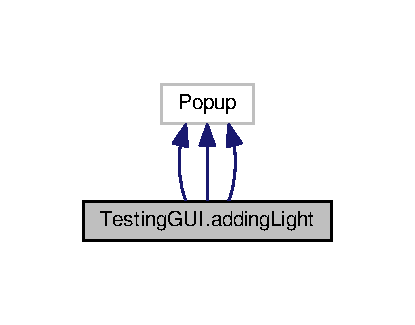
\includegraphics[width=199pt]{classTestingGUI_1_1addingLight__inherit__graph}
\end{center}
\end{figure}


Collaboration diagram for Testing\+G\+U\+I.\+adding\+Light\+:\nopagebreak
\begin{figure}[H]
\begin{center}
\leavevmode
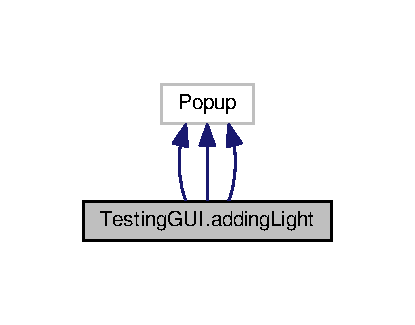
\includegraphics[width=199pt]{classTestingGUI_1_1addingLight__coll__graph}
\end{center}
\end{figure}
\subsection*{Public Member Functions}
\begin{DoxyCompactItemize}
\item 
def \hyperlink{classTestingGUI_1_1addingLight_ace8a7edfba84662f465ad3b6cc979ba0}{\+\_\+\+\_\+init\+\_\+\+\_\+} (self, kwargs)
\item 
def \hyperlink{classTestingGUI_1_1addingLight_a09539dcb1cdfd504a9e75937bf380284}{build} (self, ip\+\_\+addr, t\+\_\+data)
\item 
def \hyperlink{classTestingGUI_1_1addingLight_a4ce96f3dc2a6a06664d0c3b724dc5e8a}{add2database} (self, key, \hyperlink{classTestingGUI_1_1addingLight_afc65af761152e3325cc2cc225c9e8f7d}{ip}, \hyperlink{classTestingGUI_1_1addingLight_a763aa941465f77b12ffea9edba79c399}{data})
\item 
def \hyperlink{classTestingGUI_1_1addingLight_adec18b9e79375b11c280acdd672ea15a}{store\+\_\+name} (self, arg1)
\item 
def \hyperlink{classTestingGUI_1_1addingLight_a5804dc70f75e50f75694b529206dabf7}{initial\+\_\+\+CR} (self, ip\+\_\+address)
\item 
def \hyperlink{classTestingGUI_1_1addingLight_ace8a7edfba84662f465ad3b6cc979ba0}{\+\_\+\+\_\+init\+\_\+\+\_\+} (self, kwargs)
\item 
def \hyperlink{classTestingGUI_1_1addingLight_a09539dcb1cdfd504a9e75937bf380284}{build} (self, ip\+\_\+addr, t\+\_\+data)
\item 
def \hyperlink{classTestingGUI_1_1addingLight_a4ce96f3dc2a6a06664d0c3b724dc5e8a}{add2database} (self, key, \hyperlink{classTestingGUI_1_1addingLight_afc65af761152e3325cc2cc225c9e8f7d}{ip}, \hyperlink{classTestingGUI_1_1addingLight_a763aa941465f77b12ffea9edba79c399}{data})
\item 
def \hyperlink{classTestingGUI_1_1addingLight_adec18b9e79375b11c280acdd672ea15a}{store\+\_\+name} (self, arg1)
\item 
def \hyperlink{classTestingGUI_1_1addingLight_a5804dc70f75e50f75694b529206dabf7}{initial\+\_\+\+CR} (self, ip\+\_\+address)
\end{DoxyCompactItemize}
\subsection*{Public Attributes}
\begin{DoxyCompactItemize}
\item 
\hyperlink{classTestingGUI_1_1addingLight_a019891e6b3abbd0964de1e86a6a899e1}{textinput}
\end{DoxyCompactItemize}
\subsection*{Static Public Attributes}
\begin{DoxyCompactItemize}
\item 
string \hyperlink{classTestingGUI_1_1addingLight_ace412281b65c6556693f272d54e46da0}{keyN} = \textquotesingle{}\textquotesingle{}
\item 
string \hyperlink{classTestingGUI_1_1addingLight_afc65af761152e3325cc2cc225c9e8f7d}{ip} = \textquotesingle{}\textquotesingle{}
\item 
string \hyperlink{classTestingGUI_1_1addingLight_a763aa941465f77b12ffea9edba79c399}{data} = \textquotesingle{}\textquotesingle{}
\item 
string \hyperlink{classTestingGUI_1_1addingLight_a7e0afbbe8a8437243d79b5a296dbb36e}{bflag} = \textquotesingle{}\textquotesingle{}
\end{DoxyCompactItemize}


\subsection{Constructor \& Destructor Documentation}
\index{Testing\+G\+U\+I\+::adding\+Light@{Testing\+G\+U\+I\+::adding\+Light}!\+\_\+\+\_\+init\+\_\+\+\_\+@{\+\_\+\+\_\+init\+\_\+\+\_\+}}
\index{\+\_\+\+\_\+init\+\_\+\+\_\+@{\+\_\+\+\_\+init\+\_\+\+\_\+}!Testing\+G\+U\+I\+::adding\+Light@{Testing\+G\+U\+I\+::adding\+Light}}
\subsubsection[{\texorpdfstring{\+\_\+\+\_\+init\+\_\+\+\_\+(self, kwargs)}{__init__(self, kwargs)}}]{\setlength{\rightskip}{0pt plus 5cm}def Testing\+G\+U\+I.\+adding\+Light.\+\_\+\+\_\+init\+\_\+\+\_\+ (
\begin{DoxyParamCaption}
\item[{}]{self, }
\item[{}]{kwargs}
\end{DoxyParamCaption}
)}\hypertarget{classTestingGUI_1_1addingLight_ace8a7edfba84662f465ad3b6cc979ba0}{}\label{classTestingGUI_1_1addingLight_ace8a7edfba84662f465ad3b6cc979ba0}
\index{Testing\+G\+U\+I\+::adding\+Light@{Testing\+G\+U\+I\+::adding\+Light}!\+\_\+\+\_\+init\+\_\+\+\_\+@{\+\_\+\+\_\+init\+\_\+\+\_\+}}
\index{\+\_\+\+\_\+init\+\_\+\+\_\+@{\+\_\+\+\_\+init\+\_\+\+\_\+}!Testing\+G\+U\+I\+::adding\+Light@{Testing\+G\+U\+I\+::adding\+Light}}
\subsubsection[{\texorpdfstring{\+\_\+\+\_\+init\+\_\+\+\_\+(self, kwargs)}{__init__(self, kwargs)}}]{\setlength{\rightskip}{0pt plus 5cm}def Testing\+G\+U\+I.\+adding\+Light.\+\_\+\+\_\+init\+\_\+\+\_\+ (
\begin{DoxyParamCaption}
\item[{}]{self, }
\item[{}]{kwargs}
\end{DoxyParamCaption}
)}\hypertarget{classTestingGUI_1_1addingLight_ace8a7edfba84662f465ad3b6cc979ba0}{}\label{classTestingGUI_1_1addingLight_ace8a7edfba84662f465ad3b6cc979ba0}


\subsection{Member Function Documentation}
\index{Testing\+G\+U\+I\+::adding\+Light@{Testing\+G\+U\+I\+::adding\+Light}!add2database@{add2database}}
\index{add2database@{add2database}!Testing\+G\+U\+I\+::adding\+Light@{Testing\+G\+U\+I\+::adding\+Light}}
\subsubsection[{\texorpdfstring{add2database(self, key, ip, data)}{add2database(self, key, ip, data)}}]{\setlength{\rightskip}{0pt plus 5cm}def Testing\+G\+U\+I.\+adding\+Light.\+add2database (
\begin{DoxyParamCaption}
\item[{}]{self, }
\item[{}]{key, }
\item[{}]{ip, }
\item[{}]{data}
\end{DoxyParamCaption}
)}\hypertarget{classTestingGUI_1_1addingLight_a4ce96f3dc2a6a06664d0c3b724dc5e8a}{}\label{classTestingGUI_1_1addingLight_a4ce96f3dc2a6a06664d0c3b724dc5e8a}
\index{Testing\+G\+U\+I\+::adding\+Light@{Testing\+G\+U\+I\+::adding\+Light}!add2database@{add2database}}
\index{add2database@{add2database}!Testing\+G\+U\+I\+::adding\+Light@{Testing\+G\+U\+I\+::adding\+Light}}
\subsubsection[{\texorpdfstring{add2database(self, key, ip, data)}{add2database(self, key, ip, data)}}]{\setlength{\rightskip}{0pt plus 5cm}def Testing\+G\+U\+I.\+adding\+Light.\+add2database (
\begin{DoxyParamCaption}
\item[{}]{self, }
\item[{}]{key, }
\item[{}]{ip, }
\item[{}]{data}
\end{DoxyParamCaption}
)}\hypertarget{classTestingGUI_1_1addingLight_a4ce96f3dc2a6a06664d0c3b724dc5e8a}{}\label{classTestingGUI_1_1addingLight_a4ce96f3dc2a6a06664d0c3b724dc5e8a}
\index{Testing\+G\+U\+I\+::adding\+Light@{Testing\+G\+U\+I\+::adding\+Light}!build@{build}}
\index{build@{build}!Testing\+G\+U\+I\+::adding\+Light@{Testing\+G\+U\+I\+::adding\+Light}}
\subsubsection[{\texorpdfstring{build(self, ip\+\_\+addr, t\+\_\+data)}{build(self, ip_addr, t_data)}}]{\setlength{\rightskip}{0pt plus 5cm}def Testing\+G\+U\+I.\+adding\+Light.\+build (
\begin{DoxyParamCaption}
\item[{}]{self, }
\item[{}]{ip\+\_\+addr, }
\item[{}]{t\+\_\+data}
\end{DoxyParamCaption}
)}\hypertarget{classTestingGUI_1_1addingLight_a09539dcb1cdfd504a9e75937bf380284}{}\label{classTestingGUI_1_1addingLight_a09539dcb1cdfd504a9e75937bf380284}
\index{Testing\+G\+U\+I\+::adding\+Light@{Testing\+G\+U\+I\+::adding\+Light}!build@{build}}
\index{build@{build}!Testing\+G\+U\+I\+::adding\+Light@{Testing\+G\+U\+I\+::adding\+Light}}
\subsubsection[{\texorpdfstring{build(self, ip\+\_\+addr, t\+\_\+data)}{build(self, ip_addr, t_data)}}]{\setlength{\rightskip}{0pt plus 5cm}def Testing\+G\+U\+I.\+adding\+Light.\+build (
\begin{DoxyParamCaption}
\item[{}]{self, }
\item[{}]{ip\+\_\+addr, }
\item[{}]{t\+\_\+data}
\end{DoxyParamCaption}
)}\hypertarget{classTestingGUI_1_1addingLight_a09539dcb1cdfd504a9e75937bf380284}{}\label{classTestingGUI_1_1addingLight_a09539dcb1cdfd504a9e75937bf380284}
\index{Testing\+G\+U\+I\+::adding\+Light@{Testing\+G\+U\+I\+::adding\+Light}!initial\+\_\+\+CR@{initial\+\_\+\+CR}}
\index{initial\+\_\+\+CR@{initial\+\_\+\+CR}!Testing\+G\+U\+I\+::adding\+Light@{Testing\+G\+U\+I\+::adding\+Light}}
\subsubsection[{\texorpdfstring{initial\+\_\+\+C\+R(self, ip\+\_\+address)}{initial_CR(self, ip_address)}}]{\setlength{\rightskip}{0pt plus 5cm}def Testing\+G\+U\+I.\+adding\+Light.\+initial\+\_\+\+CR (
\begin{DoxyParamCaption}
\item[{}]{self, }
\item[{}]{ip\+\_\+address}
\end{DoxyParamCaption}
)}\hypertarget{classTestingGUI_1_1addingLight_a5804dc70f75e50f75694b529206dabf7}{}\label{classTestingGUI_1_1addingLight_a5804dc70f75e50f75694b529206dabf7}
\index{Testing\+G\+U\+I\+::adding\+Light@{Testing\+G\+U\+I\+::adding\+Light}!initial\+\_\+\+CR@{initial\+\_\+\+CR}}
\index{initial\+\_\+\+CR@{initial\+\_\+\+CR}!Testing\+G\+U\+I\+::adding\+Light@{Testing\+G\+U\+I\+::adding\+Light}}
\subsubsection[{\texorpdfstring{initial\+\_\+\+C\+R(self, ip\+\_\+address)}{initial_CR(self, ip_address)}}]{\setlength{\rightskip}{0pt plus 5cm}def Testing\+G\+U\+I.\+adding\+Light.\+initial\+\_\+\+CR (
\begin{DoxyParamCaption}
\item[{}]{self, }
\item[{}]{ip\+\_\+address}
\end{DoxyParamCaption}
)}\hypertarget{classTestingGUI_1_1addingLight_a5804dc70f75e50f75694b529206dabf7}{}\label{classTestingGUI_1_1addingLight_a5804dc70f75e50f75694b529206dabf7}
\index{Testing\+G\+U\+I\+::adding\+Light@{Testing\+G\+U\+I\+::adding\+Light}!store\+\_\+name@{store\+\_\+name}}
\index{store\+\_\+name@{store\+\_\+name}!Testing\+G\+U\+I\+::adding\+Light@{Testing\+G\+U\+I\+::adding\+Light}}
\subsubsection[{\texorpdfstring{store\+\_\+name(self, arg1)}{store_name(self, arg1)}}]{\setlength{\rightskip}{0pt plus 5cm}def Testing\+G\+U\+I.\+adding\+Light.\+store\+\_\+name (
\begin{DoxyParamCaption}
\item[{}]{self, }
\item[{}]{arg1}
\end{DoxyParamCaption}
)}\hypertarget{classTestingGUI_1_1addingLight_adec18b9e79375b11c280acdd672ea15a}{}\label{classTestingGUI_1_1addingLight_adec18b9e79375b11c280acdd672ea15a}
\index{Testing\+G\+U\+I\+::adding\+Light@{Testing\+G\+U\+I\+::adding\+Light}!store\+\_\+name@{store\+\_\+name}}
\index{store\+\_\+name@{store\+\_\+name}!Testing\+G\+U\+I\+::adding\+Light@{Testing\+G\+U\+I\+::adding\+Light}}
\subsubsection[{\texorpdfstring{store\+\_\+name(self, arg1)}{store_name(self, arg1)}}]{\setlength{\rightskip}{0pt plus 5cm}def Testing\+G\+U\+I.\+adding\+Light.\+store\+\_\+name (
\begin{DoxyParamCaption}
\item[{}]{self, }
\item[{}]{arg1}
\end{DoxyParamCaption}
)}\hypertarget{classTestingGUI_1_1addingLight_adec18b9e79375b11c280acdd672ea15a}{}\label{classTestingGUI_1_1addingLight_adec18b9e79375b11c280acdd672ea15a}


\subsection{Member Data Documentation}
\index{Testing\+G\+U\+I\+::adding\+Light@{Testing\+G\+U\+I\+::adding\+Light}!bflag@{bflag}}
\index{bflag@{bflag}!Testing\+G\+U\+I\+::adding\+Light@{Testing\+G\+U\+I\+::adding\+Light}}
\subsubsection[{\texorpdfstring{bflag}{bflag}}]{\setlength{\rightskip}{0pt plus 5cm}string Testing\+G\+U\+I.\+adding\+Light.\+bflag = \textquotesingle{}\textquotesingle{}\hspace{0.3cm}{\ttfamily [static]}}\hypertarget{classTestingGUI_1_1addingLight_a7e0afbbe8a8437243d79b5a296dbb36e}{}\label{classTestingGUI_1_1addingLight_a7e0afbbe8a8437243d79b5a296dbb36e}
\index{Testing\+G\+U\+I\+::adding\+Light@{Testing\+G\+U\+I\+::adding\+Light}!data@{data}}
\index{data@{data}!Testing\+G\+U\+I\+::adding\+Light@{Testing\+G\+U\+I\+::adding\+Light}}
\subsubsection[{\texorpdfstring{data}{data}}]{\setlength{\rightskip}{0pt plus 5cm}string Testing\+G\+U\+I.\+adding\+Light.\+data = \textquotesingle{}\textquotesingle{}\hspace{0.3cm}{\ttfamily [static]}}\hypertarget{classTestingGUI_1_1addingLight_a763aa941465f77b12ffea9edba79c399}{}\label{classTestingGUI_1_1addingLight_a763aa941465f77b12ffea9edba79c399}
\index{Testing\+G\+U\+I\+::adding\+Light@{Testing\+G\+U\+I\+::adding\+Light}!ip@{ip}}
\index{ip@{ip}!Testing\+G\+U\+I\+::adding\+Light@{Testing\+G\+U\+I\+::adding\+Light}}
\subsubsection[{\texorpdfstring{ip}{ip}}]{\setlength{\rightskip}{0pt plus 5cm}string Testing\+G\+U\+I.\+adding\+Light.\+ip = \textquotesingle{}\textquotesingle{}\hspace{0.3cm}{\ttfamily [static]}}\hypertarget{classTestingGUI_1_1addingLight_afc65af761152e3325cc2cc225c9e8f7d}{}\label{classTestingGUI_1_1addingLight_afc65af761152e3325cc2cc225c9e8f7d}
\index{Testing\+G\+U\+I\+::adding\+Light@{Testing\+G\+U\+I\+::adding\+Light}!keyN@{keyN}}
\index{keyN@{keyN}!Testing\+G\+U\+I\+::adding\+Light@{Testing\+G\+U\+I\+::adding\+Light}}
\subsubsection[{\texorpdfstring{keyN}{keyN}}]{\setlength{\rightskip}{0pt plus 5cm}string Testing\+G\+U\+I.\+adding\+Light.\+keyN = \textquotesingle{}\textquotesingle{}\hspace{0.3cm}{\ttfamily [static]}}\hypertarget{classTestingGUI_1_1addingLight_ace412281b65c6556693f272d54e46da0}{}\label{classTestingGUI_1_1addingLight_ace412281b65c6556693f272d54e46da0}
\index{Testing\+G\+U\+I\+::adding\+Light@{Testing\+G\+U\+I\+::adding\+Light}!textinput@{textinput}}
\index{textinput@{textinput}!Testing\+G\+U\+I\+::adding\+Light@{Testing\+G\+U\+I\+::adding\+Light}}
\subsubsection[{\texorpdfstring{textinput}{textinput}}]{\setlength{\rightskip}{0pt plus 5cm}Testing\+G\+U\+I.\+adding\+Light.\+textinput}\hypertarget{classTestingGUI_1_1addingLight_a019891e6b3abbd0964de1e86a6a899e1}{}\label{classTestingGUI_1_1addingLight_a019891e6b3abbd0964de1e86a6a899e1}


The documentation for this class was generated from the following file\+:\begin{DoxyCompactItemize}
\item 
/home/jac0656/\+Desktop/\+J-\/\+O-\/\+R-\/\+G-\/\+E/\+U\+N\+T-\/\+N\+A\+S\+A/\+G\+U\+I/\hyperlink{GUI_2TestingGUI_8py}{Testing\+G\+U\+I.\+py}\end{DoxyCompactItemize}

\hypertarget{classGUI8-5pm_1_1Blank}{}\section{G\+U\+I8-\/5pm.Blank Class Reference}
\label{classGUI8-5pm_1_1Blank}\index{G\+U\+I8-\/5pm.\+Blank@{G\+U\+I8-\/5pm.\+Blank}}


Inheritance diagram for G\+U\+I8-\/5pm.Blank\+:
\nopagebreak
\begin{figure}[H]
\begin{center}
\leavevmode
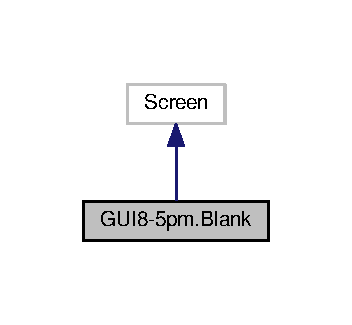
\includegraphics[width=169pt]{classGUI8-5pm_1_1Blank__inherit__graph}
\end{center}
\end{figure}


Collaboration diagram for G\+U\+I8-\/5pm.Blank\+:
\nopagebreak
\begin{figure}[H]
\begin{center}
\leavevmode
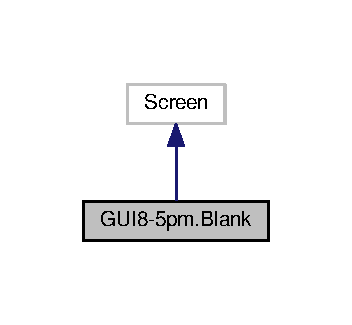
\includegraphics[width=169pt]{classGUI8-5pm_1_1Blank__coll__graph}
\end{center}
\end{figure}


The documentation for this class was generated from the following file\+:\begin{DoxyCompactItemize}
\item 
/home/jac0656/\+Desktop/\+J-\/\+O-\/\+R-\/\+G-\/\+E/\+U\+N\+T-\/\+N\+A\+S\+A/\hyperlink{GUI8-5pm_8py}{G\+U\+I8-\/5pm.\+py}\end{DoxyCompactItemize}

\hypertarget{classweb_1_1CefBrowserApp}{}\section{web.\+Cef\+Browser\+App Class Reference}
\label{classweb_1_1CefBrowserApp}\index{web.\+Cef\+Browser\+App@{web.\+Cef\+Browser\+App}}


Inheritance diagram for web.\+Cef\+Browser\+App\+:
\nopagebreak
\begin{figure}[H]
\begin{center}
\leavevmode
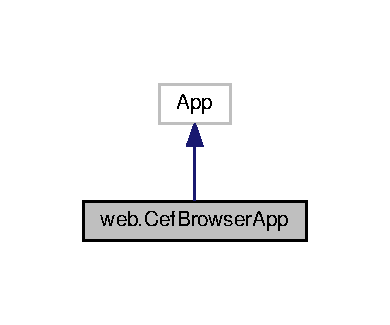
\includegraphics[width=187pt]{classweb_1_1CefBrowserApp__inherit__graph}
\end{center}
\end{figure}


Collaboration diagram for web.\+Cef\+Browser\+App\+:
\nopagebreak
\begin{figure}[H]
\begin{center}
\leavevmode
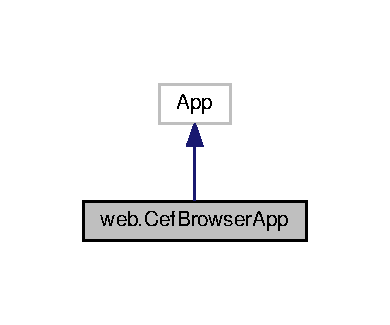
\includegraphics[width=187pt]{classweb_1_1CefBrowserApp__coll__graph}
\end{center}
\end{figure}
\subsection*{Public Member Functions}
\begin{DoxyCompactItemize}
\item 
def \hyperlink{classweb_1_1CefBrowserApp_a681fd55cb33b91bdc6013792240029a5}{build} (self)
\end{DoxyCompactItemize}


\subsection{Member Function Documentation}
\index{web\+::\+Cef\+Browser\+App@{web\+::\+Cef\+Browser\+App}!build@{build}}
\index{build@{build}!web\+::\+Cef\+Browser\+App@{web\+::\+Cef\+Browser\+App}}
\subsubsection[{\texorpdfstring{build(self)}{build(self)}}]{\setlength{\rightskip}{0pt plus 5cm}def web.\+Cef\+Browser\+App.\+build (
\begin{DoxyParamCaption}
\item[{}]{self}
\end{DoxyParamCaption}
)}\hypertarget{classweb_1_1CefBrowserApp_a681fd55cb33b91bdc6013792240029a5}{}\label{classweb_1_1CefBrowserApp_a681fd55cb33b91bdc6013792240029a5}


The documentation for this class was generated from the following file\+:\begin{DoxyCompactItemize}
\item 
/home/jac0656/\+Desktop/\+J-\/\+O-\/\+R-\/\+G-\/\+E/\+U\+N\+T-\/\+N\+A\+S\+A/\hyperlink{web_8py}{web.\+py}\end{DoxyCompactItemize}

\hypertarget{classnewGUI_1_1ColorSelector}{}\section{new\+G\+U\+I.\+Color\+Selector Class Reference}
\label{classnewGUI_1_1ColorSelector}\index{new\+G\+U\+I.\+Color\+Selector@{new\+G\+U\+I.\+Color\+Selector}}


Inheritance diagram for new\+G\+U\+I.\+Color\+Selector\+:\nopagebreak
\begin{figure}[H]
\begin{center}
\leavevmode
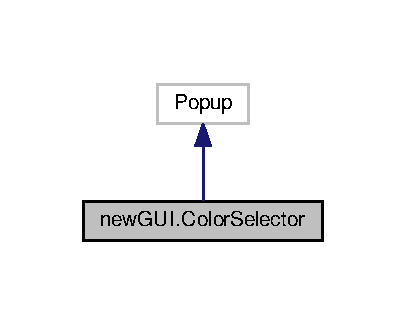
\includegraphics[width=195pt]{classnewGUI_1_1ColorSelector__inherit__graph}
\end{center}
\end{figure}


Collaboration diagram for new\+G\+U\+I.\+Color\+Selector\+:\nopagebreak
\begin{figure}[H]
\begin{center}
\leavevmode
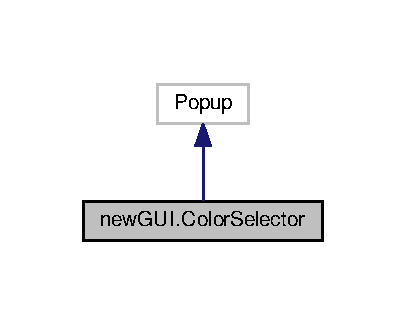
\includegraphics[width=195pt]{classnewGUI_1_1ColorSelector__coll__graph}
\end{center}
\end{figure}
\subsection*{Public Member Functions}
\begin{DoxyCompactItemize}
\item 
def \hyperlink{classnewGUI_1_1ColorSelector_a273d922b2792916abc4be0761209bc94}{on\+\_\+press\+\_\+dismiss} (self, color\+Picker, args)
\end{DoxyCompactItemize}
\subsection*{Static Public Attributes}
\begin{DoxyCompactItemize}
\item 
string \hyperlink{classnewGUI_1_1ColorSelector_a13ddd2062c3a0a3c5cd4382914c89280}{dt} = \char`\"{}\%s.\%03d\char`\"{}
\end{DoxyCompactItemize}


\subsection{Detailed Description}
\begin{DoxyVerb}This method adds the selected colors to the workfile.txt\end{DoxyVerb}
 

\subsection{Member Function Documentation}
\index{new\+G\+U\+I\+::\+Color\+Selector@{new\+G\+U\+I\+::\+Color\+Selector}!on\+\_\+press\+\_\+dismiss@{on\+\_\+press\+\_\+dismiss}}
\index{on\+\_\+press\+\_\+dismiss@{on\+\_\+press\+\_\+dismiss}!new\+G\+U\+I\+::\+Color\+Selector@{new\+G\+U\+I\+::\+Color\+Selector}}
\subsubsection[{\texorpdfstring{on\+\_\+press\+\_\+dismiss(self, color\+Picker, args)}{on_press_dismiss(self, colorPicker, args)}}]{\setlength{\rightskip}{0pt plus 5cm}def new\+G\+U\+I.\+Color\+Selector.\+on\+\_\+press\+\_\+dismiss (
\begin{DoxyParamCaption}
\item[{}]{self, }
\item[{}]{color\+Picker, }
\item[{}]{args}
\end{DoxyParamCaption}
)}\hypertarget{classnewGUI_1_1ColorSelector_a273d922b2792916abc4be0761209bc94}{}\label{classnewGUI_1_1ColorSelector_a273d922b2792916abc4be0761209bc94}


\subsection{Member Data Documentation}
\index{new\+G\+U\+I\+::\+Color\+Selector@{new\+G\+U\+I\+::\+Color\+Selector}!dt@{dt}}
\index{dt@{dt}!new\+G\+U\+I\+::\+Color\+Selector@{new\+G\+U\+I\+::\+Color\+Selector}}
\subsubsection[{\texorpdfstring{dt}{dt}}]{\setlength{\rightskip}{0pt plus 5cm}string new\+G\+U\+I.\+Color\+Selector.\+dt = \char`\"{}\%s.\%03d\char`\"{}\hspace{0.3cm}{\ttfamily [static]}}\hypertarget{classnewGUI_1_1ColorSelector_a13ddd2062c3a0a3c5cd4382914c89280}{}\label{classnewGUI_1_1ColorSelector_a13ddd2062c3a0a3c5cd4382914c89280}


The documentation for this class was generated from the following file\+:\begin{DoxyCompactItemize}
\item 
/home/jac0656/\+Desktop/\+J-\/\+O-\/\+R-\/\+G-\/\+E/\+U\+N\+T-\/\+N\+A\+S\+A/\+G\+U\+I/\hyperlink{newGUI_8py}{new\+G\+U\+I.\+py}\end{DoxyCompactItemize}

\hypertarget{classGUI8_1_1ColorSelector}{}\section{G\+U\+I8.\+Color\+Selector Class Reference}
\label{classGUI8_1_1ColorSelector}\index{G\+U\+I8.\+Color\+Selector@{G\+U\+I8.\+Color\+Selector}}


Inheritance diagram for G\+U\+I8.\+Color\+Selector\+:
\nopagebreak
\begin{figure}[H]
\begin{center}
\leavevmode
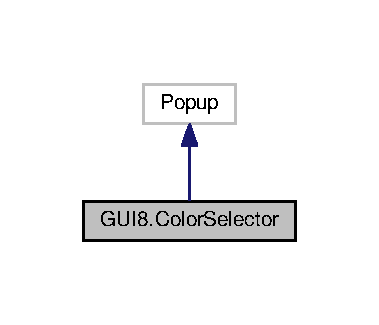
\includegraphics[width=182pt]{classGUI8_1_1ColorSelector__inherit__graph}
\end{center}
\end{figure}


Collaboration diagram for G\+U\+I8.\+Color\+Selector\+:
\nopagebreak
\begin{figure}[H]
\begin{center}
\leavevmode
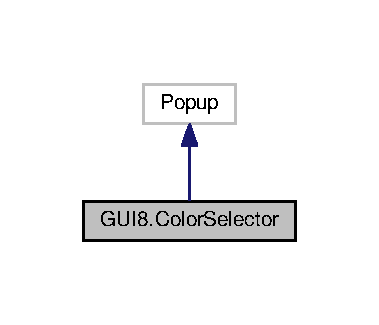
\includegraphics[width=182pt]{classGUI8_1_1ColorSelector__coll__graph}
\end{center}
\end{figure}
\subsection*{Public Member Functions}
\begin{DoxyCompactItemize}
\item 
def \hyperlink{classGUI8_1_1ColorSelector_af1c3dc2b6ada3189e0d69d7a16c347a7}{on\+\_\+press\+\_\+dismiss} (self, color\+Picker, args)
\end{DoxyCompactItemize}
\subsection*{Static Public Attributes}
\begin{DoxyCompactItemize}
\item 
string \hyperlink{classGUI8_1_1ColorSelector_af1a5f907f08fe7e2078ac767df1addb4}{dt} = \char`\"{}\%s.\%03d\char`\"{}
\end{DoxyCompactItemize}


\subsection{Member Function Documentation}
\index{G\+U\+I8\+::\+Color\+Selector@{G\+U\+I8\+::\+Color\+Selector}!on\+\_\+press\+\_\+dismiss@{on\+\_\+press\+\_\+dismiss}}
\index{on\+\_\+press\+\_\+dismiss@{on\+\_\+press\+\_\+dismiss}!G\+U\+I8\+::\+Color\+Selector@{G\+U\+I8\+::\+Color\+Selector}}
\subsubsection[{\texorpdfstring{on\+\_\+press\+\_\+dismiss(self, color\+Picker, args)}{on_press_dismiss(self, colorPicker, args)}}]{\setlength{\rightskip}{0pt plus 5cm}def G\+U\+I8.\+Color\+Selector.\+on\+\_\+press\+\_\+dismiss (
\begin{DoxyParamCaption}
\item[{}]{self, }
\item[{}]{color\+Picker, }
\item[{}]{args}
\end{DoxyParamCaption}
)}\hypertarget{classGUI8_1_1ColorSelector_af1c3dc2b6ada3189e0d69d7a16c347a7}{}\label{classGUI8_1_1ColorSelector_af1c3dc2b6ada3189e0d69d7a16c347a7}


\subsection{Member Data Documentation}
\index{G\+U\+I8\+::\+Color\+Selector@{G\+U\+I8\+::\+Color\+Selector}!dt@{dt}}
\index{dt@{dt}!G\+U\+I8\+::\+Color\+Selector@{G\+U\+I8\+::\+Color\+Selector}}
\subsubsection[{\texorpdfstring{dt}{dt}}]{\setlength{\rightskip}{0pt plus 5cm}string G\+U\+I8.\+Color\+Selector.\+dt = \char`\"{}\%s.\%03d\char`\"{}\hspace{0.3cm}{\ttfamily [static]}}\hypertarget{classGUI8_1_1ColorSelector_af1a5f907f08fe7e2078ac767df1addb4}{}\label{classGUI8_1_1ColorSelector_af1a5f907f08fe7e2078ac767df1addb4}


The documentation for this class was generated from the following file\+:\begin{DoxyCompactItemize}
\item 
/home/jac0656/\+Desktop/\+J-\/\+O-\/\+R-\/\+G-\/\+E/\+U\+N\+T-\/\+N\+A\+S\+A/\+G\+U\+I/\hyperlink{GUI8_8py}{G\+U\+I8.\+py}\end{DoxyCompactItemize}

\hypertarget{classGUI8-5pm_1_1ColorSelector}{}\section{G\+U\+I8-\/5pm.Color\+Selector Class Reference}
\label{classGUI8-5pm_1_1ColorSelector}\index{G\+U\+I8-\/5pm.\+Color\+Selector@{G\+U\+I8-\/5pm.\+Color\+Selector}}


Inheritance diagram for G\+U\+I8-\/5pm.Color\+Selector\+:\nopagebreak
\begin{figure}[H]
\begin{center}
\leavevmode
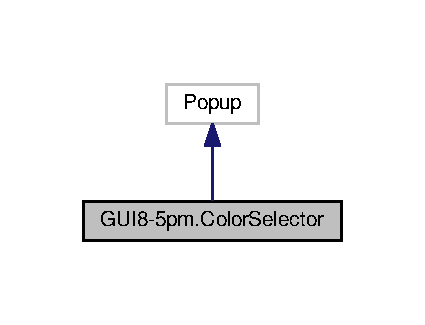
\includegraphics[width=204pt]{classGUI8-5pm_1_1ColorSelector__inherit__graph}
\end{center}
\end{figure}


Collaboration diagram for G\+U\+I8-\/5pm.Color\+Selector\+:\nopagebreak
\begin{figure}[H]
\begin{center}
\leavevmode
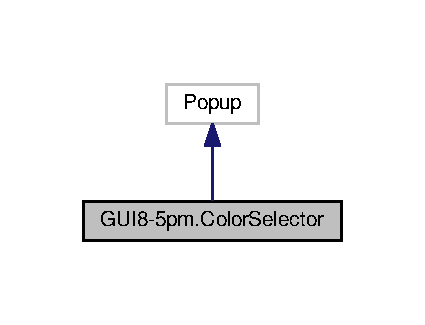
\includegraphics[width=204pt]{classGUI8-5pm_1_1ColorSelector__coll__graph}
\end{center}
\end{figure}
\subsection*{Public Member Functions}
\begin{DoxyCompactItemize}
\item 
def \hyperlink{classGUI8-5pm_1_1ColorSelector_ad066b578ca09bc8910db73c32741b8f8}{on\+\_\+press\+\_\+dismiss} (self, color\+Picker, args)
\end{DoxyCompactItemize}
\subsection*{Static Public Attributes}
\begin{DoxyCompactItemize}
\item 
string \hyperlink{classGUI8-5pm_1_1ColorSelector_a757632868adf77e3170d9d45d69e2ef9}{dt} = \char`\"{}\%s.\%03d\char`\"{}
\end{DoxyCompactItemize}


\subsection{Detailed Description}
\begin{DoxyVerb}This is the method that gets called when the user presses OK on the color wheel. It stores those values on the DB\end{DoxyVerb}
 

\subsection{Member Function Documentation}
\index{G\+U\+I8-\/5pm\+::\+Color\+Selector@{G\+U\+I8-\/5pm\+::\+Color\+Selector}!on\+\_\+press\+\_\+dismiss@{on\+\_\+press\+\_\+dismiss}}
\index{on\+\_\+press\+\_\+dismiss@{on\+\_\+press\+\_\+dismiss}!G\+U\+I8-\/5pm\+::\+Color\+Selector@{G\+U\+I8-\/5pm\+::\+Color\+Selector}}
\subsubsection[{\texorpdfstring{on\+\_\+press\+\_\+dismiss(self, color\+Picker, args)}{on_press_dismiss(self, colorPicker, args)}}]{\setlength{\rightskip}{0pt plus 5cm}def G\+U\+I8-\/5pm.\+Color\+Selector.\+on\+\_\+press\+\_\+dismiss (
\begin{DoxyParamCaption}
\item[{}]{self, }
\item[{}]{color\+Picker, }
\item[{}]{args}
\end{DoxyParamCaption}
)}\hypertarget{classGUI8-5pm_1_1ColorSelector_ad066b578ca09bc8910db73c32741b8f8}{}\label{classGUI8-5pm_1_1ColorSelector_ad066b578ca09bc8910db73c32741b8f8}


\subsection{Member Data Documentation}
\index{G\+U\+I8-\/5pm\+::\+Color\+Selector@{G\+U\+I8-\/5pm\+::\+Color\+Selector}!dt@{dt}}
\index{dt@{dt}!G\+U\+I8-\/5pm\+::\+Color\+Selector@{G\+U\+I8-\/5pm\+::\+Color\+Selector}}
\subsubsection[{\texorpdfstring{dt}{dt}}]{\setlength{\rightskip}{0pt plus 5cm}string G\+U\+I8-\/5pm.\+Color\+Selector.\+dt = \char`\"{}\%s.\%03d\char`\"{}\hspace{0.3cm}{\ttfamily [static]}}\hypertarget{classGUI8-5pm_1_1ColorSelector_a757632868adf77e3170d9d45d69e2ef9}{}\label{classGUI8-5pm_1_1ColorSelector_a757632868adf77e3170d9d45d69e2ef9}


The documentation for this class was generated from the following file\+:\begin{DoxyCompactItemize}
\item 
/home/jac0656/\+Desktop/\+J-\/\+O-\/\+R-\/\+G-\/\+E/\+U\+N\+T-\/\+N\+A\+S\+A/\hyperlink{GUI8-5pm_8py}{G\+U\+I8-\/5pm.\+py}\end{DoxyCompactItemize}

\hypertarget{classTestApp1_1_1ColorSelector}{}\section{Test\+App1.\+Color\+Selector Class Reference}
\label{classTestApp1_1_1ColorSelector}\index{Test\+App1.\+Color\+Selector@{Test\+App1.\+Color\+Selector}}


Inheritance diagram for Test\+App1.\+Color\+Selector\+:
\nopagebreak
\begin{figure}[H]
\begin{center}
\leavevmode
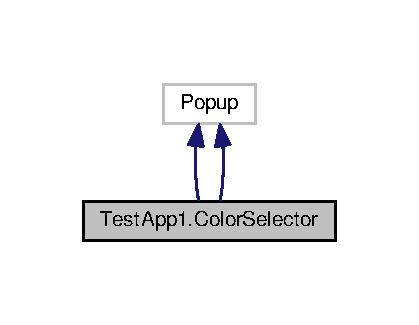
\includegraphics[width=201pt]{classTestApp1_1_1ColorSelector__inherit__graph}
\end{center}
\end{figure}


Collaboration diagram for Test\+App1.\+Color\+Selector\+:
\nopagebreak
\begin{figure}[H]
\begin{center}
\leavevmode
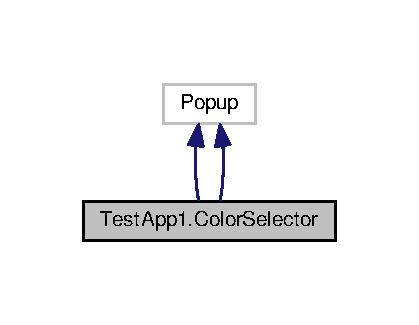
\includegraphics[width=201pt]{classTestApp1_1_1ColorSelector__coll__graph}
\end{center}
\end{figure}
\subsection*{Public Member Functions}
\begin{DoxyCompactItemize}
\item 
def \hyperlink{classTestApp1_1_1ColorSelector_afcecec797d6c063981dd5c29a6b876a3}{on\+\_\+press\+\_\+dismiss} (self, color\+Picker, args)
\item 
def \hyperlink{classTestApp1_1_1ColorSelector_afcecec797d6c063981dd5c29a6b876a3}{on\+\_\+press\+\_\+dismiss} (self, color\+Picker, args)
\end{DoxyCompactItemize}


\subsection{Member Function Documentation}
\index{Test\+App1\+::\+Color\+Selector@{Test\+App1\+::\+Color\+Selector}!on\+\_\+press\+\_\+dismiss@{on\+\_\+press\+\_\+dismiss}}
\index{on\+\_\+press\+\_\+dismiss@{on\+\_\+press\+\_\+dismiss}!Test\+App1\+::\+Color\+Selector@{Test\+App1\+::\+Color\+Selector}}
\subsubsection[{\texorpdfstring{on\+\_\+press\+\_\+dismiss(self, color\+Picker, args)}{on_press_dismiss(self, colorPicker, args)}}]{\setlength{\rightskip}{0pt plus 5cm}def Test\+App1.\+Color\+Selector.\+on\+\_\+press\+\_\+dismiss (
\begin{DoxyParamCaption}
\item[{}]{self, }
\item[{}]{color\+Picker, }
\item[{}]{args}
\end{DoxyParamCaption}
)}\hypertarget{classTestApp1_1_1ColorSelector_afcecec797d6c063981dd5c29a6b876a3}{}\label{classTestApp1_1_1ColorSelector_afcecec797d6c063981dd5c29a6b876a3}
\index{Test\+App1\+::\+Color\+Selector@{Test\+App1\+::\+Color\+Selector}!on\+\_\+press\+\_\+dismiss@{on\+\_\+press\+\_\+dismiss}}
\index{on\+\_\+press\+\_\+dismiss@{on\+\_\+press\+\_\+dismiss}!Test\+App1\+::\+Color\+Selector@{Test\+App1\+::\+Color\+Selector}}
\subsubsection[{\texorpdfstring{on\+\_\+press\+\_\+dismiss(self, color\+Picker, args)}{on_press_dismiss(self, colorPicker, args)}}]{\setlength{\rightskip}{0pt plus 5cm}def Test\+App1.\+Color\+Selector.\+on\+\_\+press\+\_\+dismiss (
\begin{DoxyParamCaption}
\item[{}]{self, }
\item[{}]{color\+Picker, }
\item[{}]{args}
\end{DoxyParamCaption}
)}\hypertarget{classTestApp1_1_1ColorSelector_afcecec797d6c063981dd5c29a6b876a3}{}\label{classTestApp1_1_1ColorSelector_afcecec797d6c063981dd5c29a6b876a3}


The documentation for this class was generated from the following file\+:\begin{DoxyCompactItemize}
\item 
/home/jac0656/\+Desktop/\+J-\/\+O-\/\+R-\/\+G-\/\+E/\+U\+N\+T-\/\+N\+A\+S\+A/\+Outreach/\hyperlink{Outreach_2TestApp1_8py}{Test\+App1.\+py}\end{DoxyCompactItemize}

\hypertarget{classDMX512}{}\section{D\+M\+X512 Class Reference}
\label{classDMX512}\index{D\+M\+X512@{D\+M\+X512}}


{\ttfamily \#include $<$dmx512.\+hpp$>$}

\subsection*{Public Member Functions}
\begin{DoxyCompactItemize}
\item 
\hyperlink{classDMX512_a20a4e33b35609a6e1ac54b5812f6704b}{D\+M\+X512} ()
\item 
void \hyperlink{classDMX512_ad392198ed2202ea28a78764ba1d9c453}{set\+Out\+Of\+Range} (int i)
\item 
int \hyperlink{classDMX512_aebc0e33cf9e594124b3a48f86bd6a95c}{get\+Out\+Of\+Range} ()
\item 
void \hyperlink{classDMX512_af7b430f6b8c50ad34773c2f83eaa3db9}{set\+Data} (std\+::string D\+A\+TA)
\item 
void \hyperlink{classDMX512_a6ae50e79301e42784934bf853c945b45}{client\+Handler} ()
\item 
std\+::string \hyperlink{classDMX512_adb00c53d6367188e848fea660d31da28}{send\+O\+LA} ()
\item 
void \hyperlink{classDMX512_a12731a1553eed443a1ebbc6aa7e92864}{check\+O\+LA} ()
\end{DoxyCompactItemize}
\subsection*{Public Attributes}
\begin{DoxyCompactItemize}
\item 
std\+::string \hyperlink{classDMX512_a51cddf44923b3cd81ad448b461315c1d}{A}
\item 
std\+::string \hyperlink{classDMX512_a231a85f100b6b81a202143d858ed26d1}{R}
\item 
std\+::string \hyperlink{classDMX512_ae7d4142513f8c3978c93f39bf5c1c599}{G}
\item 
std\+::string \hyperlink{classDMX512_af3306a5965828c8eb012e2d570f7614e}{B}
\item 
std\+::string \hyperlink{classDMX512_a266eca0f1d1836e8122edd5efeae3c84}{O\+LA}
\item 
unsigned int \hyperlink{classDMX512_ae450756118a5e3d1173fd564deeb11c3}{Ai}
\item 
unsigned int \hyperlink{classDMX512_aa5ffc37b24d0a79180d13663a5cf8379}{Ri}
\item 
unsigned int \hyperlink{classDMX512_afa6a4f81386fd8c8fc86a156fc7018e1}{Gi}
\item 
unsigned int \hyperlink{classDMX512_a8f4300cb289c94e708314c1bb3078ca8}{Bi}
\end{DoxyCompactItemize}


\subsection{Constructor \& Destructor Documentation}
\index{D\+M\+X512@{D\+M\+X512}!D\+M\+X512@{D\+M\+X512}}
\index{D\+M\+X512@{D\+M\+X512}!D\+M\+X512@{D\+M\+X512}}
\subsubsection[{\texorpdfstring{D\+M\+X512()}{DMX512()}}]{\setlength{\rightskip}{0pt plus 5cm}D\+M\+X512\+::\+D\+M\+X512 (
\begin{DoxyParamCaption}
{}
\end{DoxyParamCaption}
)}\hypertarget{classDMX512_a20a4e33b35609a6e1ac54b5812f6704b}{}\label{classDMX512_a20a4e33b35609a6e1ac54b5812f6704b}


\subsection{Member Function Documentation}
\index{D\+M\+X512@{D\+M\+X512}!check\+O\+LA@{check\+O\+LA}}
\index{check\+O\+LA@{check\+O\+LA}!D\+M\+X512@{D\+M\+X512}}
\subsubsection[{\texorpdfstring{check\+O\+L\+A()}{checkOLA()}}]{\setlength{\rightskip}{0pt plus 5cm}void D\+M\+X512\+::check\+O\+LA (
\begin{DoxyParamCaption}
{}
\end{DoxyParamCaption}
)}\hypertarget{classDMX512_a12731a1553eed443a1ebbc6aa7e92864}{}\label{classDMX512_a12731a1553eed443a1ebbc6aa7e92864}
\index{D\+M\+X512@{D\+M\+X512}!client\+Handler@{client\+Handler}}
\index{client\+Handler@{client\+Handler}!D\+M\+X512@{D\+M\+X512}}
\subsubsection[{\texorpdfstring{client\+Handler()}{clientHandler()}}]{\setlength{\rightskip}{0pt plus 5cm}void D\+M\+X512\+::client\+Handler (
\begin{DoxyParamCaption}
{}
\end{DoxyParamCaption}
)}\hypertarget{classDMX512_a6ae50e79301e42784934bf853c945b45}{}\label{classDMX512_a6ae50e79301e42784934bf853c945b45}
\index{D\+M\+X512@{D\+M\+X512}!get\+Out\+Of\+Range@{get\+Out\+Of\+Range}}
\index{get\+Out\+Of\+Range@{get\+Out\+Of\+Range}!D\+M\+X512@{D\+M\+X512}}
\subsubsection[{\texorpdfstring{get\+Out\+Of\+Range()}{getOutOfRange()}}]{\setlength{\rightskip}{0pt plus 5cm}int D\+M\+X512\+::get\+Out\+Of\+Range (
\begin{DoxyParamCaption}
{}
\end{DoxyParamCaption}
)}\hypertarget{classDMX512_aebc0e33cf9e594124b3a48f86bd6a95c}{}\label{classDMX512_aebc0e33cf9e594124b3a48f86bd6a95c}
\index{D\+M\+X512@{D\+M\+X512}!send\+O\+LA@{send\+O\+LA}}
\index{send\+O\+LA@{send\+O\+LA}!D\+M\+X512@{D\+M\+X512}}
\subsubsection[{\texorpdfstring{send\+O\+L\+A()}{sendOLA()}}]{\setlength{\rightskip}{0pt plus 5cm}std\+::string D\+M\+X512\+::send\+O\+LA (
\begin{DoxyParamCaption}
{}
\end{DoxyParamCaption}
)}\hypertarget{classDMX512_adb00c53d6367188e848fea660d31da28}{}\label{classDMX512_adb00c53d6367188e848fea660d31da28}
\index{D\+M\+X512@{D\+M\+X512}!set\+Data@{set\+Data}}
\index{set\+Data@{set\+Data}!D\+M\+X512@{D\+M\+X512}}
\subsubsection[{\texorpdfstring{set\+Data(std\+::string D\+A\+T\+A)}{setData(std::string DATA)}}]{\setlength{\rightskip}{0pt plus 5cm}void D\+M\+X512\+::set\+Data (
\begin{DoxyParamCaption}
\item[{std\+::string}]{D\+A\+TA}
\end{DoxyParamCaption}
)}\hypertarget{classDMX512_af7b430f6b8c50ad34773c2f83eaa3db9}{}\label{classDMX512_af7b430f6b8c50ad34773c2f83eaa3db9}
\index{D\+M\+X512@{D\+M\+X512}!set\+Out\+Of\+Range@{set\+Out\+Of\+Range}}
\index{set\+Out\+Of\+Range@{set\+Out\+Of\+Range}!D\+M\+X512@{D\+M\+X512}}
\subsubsection[{\texorpdfstring{set\+Out\+Of\+Range(int i)}{setOutOfRange(int i)}}]{\setlength{\rightskip}{0pt plus 5cm}void D\+M\+X512\+::set\+Out\+Of\+Range (
\begin{DoxyParamCaption}
\item[{int}]{i}
\end{DoxyParamCaption}
)}\hypertarget{classDMX512_ad392198ed2202ea28a78764ba1d9c453}{}\label{classDMX512_ad392198ed2202ea28a78764ba1d9c453}


\subsection{Member Data Documentation}
\index{D\+M\+X512@{D\+M\+X512}!A@{A}}
\index{A@{A}!D\+M\+X512@{D\+M\+X512}}
\subsubsection[{\texorpdfstring{A}{A}}]{\setlength{\rightskip}{0pt plus 5cm}std\+::string D\+M\+X512\+::A}\hypertarget{classDMX512_a51cddf44923b3cd81ad448b461315c1d}{}\label{classDMX512_a51cddf44923b3cd81ad448b461315c1d}
\index{D\+M\+X512@{D\+M\+X512}!Ai@{Ai}}
\index{Ai@{Ai}!D\+M\+X512@{D\+M\+X512}}
\subsubsection[{\texorpdfstring{Ai}{Ai}}]{\setlength{\rightskip}{0pt plus 5cm}unsigned int D\+M\+X512\+::\+Ai}\hypertarget{classDMX512_ae450756118a5e3d1173fd564deeb11c3}{}\label{classDMX512_ae450756118a5e3d1173fd564deeb11c3}
\index{D\+M\+X512@{D\+M\+X512}!B@{B}}
\index{B@{B}!D\+M\+X512@{D\+M\+X512}}
\subsubsection[{\texorpdfstring{B}{B}}]{\setlength{\rightskip}{0pt plus 5cm}std\+::string D\+M\+X512\+::B}\hypertarget{classDMX512_af3306a5965828c8eb012e2d570f7614e}{}\label{classDMX512_af3306a5965828c8eb012e2d570f7614e}
\index{D\+M\+X512@{D\+M\+X512}!Bi@{Bi}}
\index{Bi@{Bi}!D\+M\+X512@{D\+M\+X512}}
\subsubsection[{\texorpdfstring{Bi}{Bi}}]{\setlength{\rightskip}{0pt plus 5cm}unsigned int D\+M\+X512\+::\+Bi}\hypertarget{classDMX512_a8f4300cb289c94e708314c1bb3078ca8}{}\label{classDMX512_a8f4300cb289c94e708314c1bb3078ca8}
\index{D\+M\+X512@{D\+M\+X512}!G@{G}}
\index{G@{G}!D\+M\+X512@{D\+M\+X512}}
\subsubsection[{\texorpdfstring{G}{G}}]{\setlength{\rightskip}{0pt plus 5cm}std\+::string D\+M\+X512\+::G}\hypertarget{classDMX512_ae7d4142513f8c3978c93f39bf5c1c599}{}\label{classDMX512_ae7d4142513f8c3978c93f39bf5c1c599}
\index{D\+M\+X512@{D\+M\+X512}!Gi@{Gi}}
\index{Gi@{Gi}!D\+M\+X512@{D\+M\+X512}}
\subsubsection[{\texorpdfstring{Gi}{Gi}}]{\setlength{\rightskip}{0pt plus 5cm}unsigned int D\+M\+X512\+::\+Gi}\hypertarget{classDMX512_afa6a4f81386fd8c8fc86a156fc7018e1}{}\label{classDMX512_afa6a4f81386fd8c8fc86a156fc7018e1}
\index{D\+M\+X512@{D\+M\+X512}!O\+LA@{O\+LA}}
\index{O\+LA@{O\+LA}!D\+M\+X512@{D\+M\+X512}}
\subsubsection[{\texorpdfstring{O\+LA}{OLA}}]{\setlength{\rightskip}{0pt plus 5cm}std\+::string D\+M\+X512\+::\+O\+LA}\hypertarget{classDMX512_a266eca0f1d1836e8122edd5efeae3c84}{}\label{classDMX512_a266eca0f1d1836e8122edd5efeae3c84}
\index{D\+M\+X512@{D\+M\+X512}!R@{R}}
\index{R@{R}!D\+M\+X512@{D\+M\+X512}}
\subsubsection[{\texorpdfstring{R}{R}}]{\setlength{\rightskip}{0pt plus 5cm}std\+::string D\+M\+X512\+::R}\hypertarget{classDMX512_a231a85f100b6b81a202143d858ed26d1}{}\label{classDMX512_a231a85f100b6b81a202143d858ed26d1}
\index{D\+M\+X512@{D\+M\+X512}!Ri@{Ri}}
\index{Ri@{Ri}!D\+M\+X512@{D\+M\+X512}}
\subsubsection[{\texorpdfstring{Ri}{Ri}}]{\setlength{\rightskip}{0pt plus 5cm}unsigned int D\+M\+X512\+::\+Ri}\hypertarget{classDMX512_aa5ffc37b24d0a79180d13663a5cf8379}{}\label{classDMX512_aa5ffc37b24d0a79180d13663a5cf8379}


The documentation for this class was generated from the following files\+:\begin{DoxyCompactItemize}
\item 
/home/jac0656/\+Desktop/\+J-\/\+O-\/\+R-\/\+G-\/\+E/\+U\+N\+T-\/\+N\+A\+S\+A/\hyperlink{dmx512_8hpp}{dmx512.\+hpp}\item 
/home/jac0656/\+Desktop/\+J-\/\+O-\/\+R-\/\+G-\/\+E/\+U\+N\+T-\/\+N\+A\+S\+A/\hyperlink{dmx512_8c_09_09}{dmx512.\+c++}\end{DoxyCompactItemize}

\hypertarget{classGUI8J_1_1Health}{}\section{G\+U\+I8\+J.\+Health Class Reference}
\label{classGUI8J_1_1Health}\index{G\+U\+I8\+J.\+Health@{G\+U\+I8\+J.\+Health}}


Inheritance diagram for G\+U\+I8\+J.\+Health\+:
% FIG 0


Collaboration diagram for G\+U\+I8\+J.\+Health\+:
% FIG 1
\subsection*{Public Member Functions}
\begin{DoxyCompactItemize}
\item 
def \hyperlink{classGUI8J_1_1Health_a6a1d62107161762df7294f37363cc3d0}{\+\_\+\+\_\+init\+\_\+\+\_\+} (self, kwargs)
\item 
def \hyperlink{classGUI8J_1_1Health_ae6f9ce7f00cf508b5265d514c83b190e}{check\+\_\+status\+\_\+\+A\+LL} (self)
\item 
def \hyperlink{classGUI8J_1_1Health_abe7fdc17fa8c4775f8d0a003895639d2}{health\+\_\+status} (self)
\item 
def \hyperlink{classGUI8J_1_1Health_ad3faaa369c1ef2c9a56e3e1d435c7fc2}{health\+\_\+popup} (self)
\item 
def \hyperlink{classGUI8J_1_1Health_a163b14e031bd548afa77530c64ebb479}{back\+\_\+to\+\_\+rv} (self, arg1)
\item 
def \hyperlink{classGUI8J_1_1Health_a52bba86fbebd0666cad9f1e1cfaf153f}{retrieve\+Sensor} (self, ip\+\_\+addr, d)
\item 
def \hyperlink{classGUI8J_1_1Health_a0c31bade8c2f9f1d5fa2321c12337466}{get\+Time} (self)
\item 
def \hyperlink{classGUI8J_1_1Health_ab2063827790ff6e6e1202a284c773ba4}{retrieve\+C\+R\+\_\+and\+\_\+status} (self, hour)
\item 
def \hyperlink{classGUI8J_1_1Health_a59855385f1bd944448ec71756e391cee}{clear\+\_\+selection} (self)
\item 
def \hyperlink{classGUI8J_1_1Health_a72e5243684cdfdfff0b7b7262dddb6d5}{status\+\_\+popup} (self)
\end{DoxyCompactItemize}
\subsection*{Static Public Attributes}
\begin{DoxyCompactItemize}
\item 
\hyperlink{classGUI8J_1_1Health_a9ba91a4c82d6eeaa9d337472eb34d196}{time} = String\+Property()
\item 
\hyperlink{classGUI8J_1_1Health_ab6cd63455568741bf222a12e30986843}{date} = String\+Property()
\item 
\hyperlink{classGUI8J_1_1Health_afe9b8605a620a4d879366b972489c906}{red} = String\+Property()
\item 
\hyperlink{classGUI8J_1_1Health_a8b1376719c2bd18543761f14a1839228}{green} = String\+Property()
\item 
\hyperlink{classGUI8J_1_1Health_a337d3e4c0e7bc4940c1adfb2d279f95a}{blue} = String\+Property()
\item 
\hyperlink{classGUI8J_1_1Health_a5b6640fd4669214a8954dd4b32485bdc}{intensity} = String\+Property()
\item 
\hyperlink{classGUI8J_1_1Health_a28566a18c87f55e0b1e167becfcd7312}{status} = String\+Property()
\item 
\hyperlink{classGUI8J_1_1Health_a41de19b60751c33a832ca7bab8d00329}{light\+\_\+name} = String\+Property()
\item 
\hyperlink{classGUI8J_1_1Health_a0744fbcfd0cda65b5dd535e2cdc60595}{ip} = String\+Property()
\item 
\hyperlink{classGUI8J_1_1Health_af614c5f4803c3772200fd6737b70700c}{sa} = String\+Property()
\item 
\hyperlink{classGUI8J_1_1Health_aff22cd911daa230907c1b365f7286e43}{sr} = String\+Property()
\item 
\hyperlink{classGUI8J_1_1Health_a3fc10d8842d9f4ddc2765c0239802c4b}{sg} = String\+Property()
\item 
\hyperlink{classGUI8J_1_1Health_a31020b4703cf26d8f44f1400c4e2781c}{sb} = String\+Property()
\item 
\hyperlink{classGUI8J_1_1Health_a994507f94a48b2dc5b2e94d1f39efd70}{A} = Numeric\+Property()
\item 
\hyperlink{classGUI8J_1_1Health_aa861a42d345235fb341865f7425953c5}{B} = Numeric\+Property()
\item 
\hyperlink{classGUI8J_1_1Health_ae3476b699f987a416e07d6576b7832fe}{R} = Numeric\+Property()
\item 
\hyperlink{classGUI8J_1_1Health_a54d41e7f742501e3c8bbc8c0de7179be}{G} = Numeric\+Property()
\end{DoxyCompactItemize}


\subsection{Constructor \& Destructor Documentation}
\mbox{\Hypertarget{classGUI8J_1_1Health_a6a1d62107161762df7294f37363cc3d0}\label{classGUI8J_1_1Health_a6a1d62107161762df7294f37363cc3d0}} 
\index{G\+U\+I8\+J\+::\+Health@{G\+U\+I8\+J\+::\+Health}!\+\_\+\+\_\+init\+\_\+\+\_\+@{\+\_\+\+\_\+init\+\_\+\+\_\+}}
\index{\+\_\+\+\_\+init\+\_\+\+\_\+@{\+\_\+\+\_\+init\+\_\+\+\_\+}!G\+U\+I8\+J\+::\+Health@{G\+U\+I8\+J\+::\+Health}}
\subsubsection{\texorpdfstring{\+\_\+\+\_\+init\+\_\+\+\_\+()}{\_\_init\_\_()}}
{\footnotesize\ttfamily def G\+U\+I8\+J.\+Health.\+\_\+\+\_\+init\+\_\+\+\_\+ (\begin{DoxyParamCaption}\item[{}]{self,  }\item[{}]{kwargs }\end{DoxyParamCaption})}



\subsection{Member Function Documentation}
\mbox{\Hypertarget{classGUI8J_1_1Health_a163b14e031bd548afa77530c64ebb479}\label{classGUI8J_1_1Health_a163b14e031bd548afa77530c64ebb479}} 
\index{G\+U\+I8\+J\+::\+Health@{G\+U\+I8\+J\+::\+Health}!back\+\_\+to\+\_\+rv@{back\+\_\+to\+\_\+rv}}
\index{back\+\_\+to\+\_\+rv@{back\+\_\+to\+\_\+rv}!G\+U\+I8\+J\+::\+Health@{G\+U\+I8\+J\+::\+Health}}
\subsubsection{\texorpdfstring{back\+\_\+to\+\_\+rv()}{back\_to\_rv()}}
{\footnotesize\ttfamily def G\+U\+I8\+J.\+Health.\+back\+\_\+to\+\_\+rv (\begin{DoxyParamCaption}\item[{}]{self,  }\item[{}]{arg1 }\end{DoxyParamCaption})}

\mbox{\Hypertarget{classGUI8J_1_1Health_ae6f9ce7f00cf508b5265d514c83b190e}\label{classGUI8J_1_1Health_ae6f9ce7f00cf508b5265d514c83b190e}} 
\index{G\+U\+I8\+J\+::\+Health@{G\+U\+I8\+J\+::\+Health}!check\+\_\+status\+\_\+\+A\+LL@{check\+\_\+status\+\_\+\+A\+LL}}
\index{check\+\_\+status\+\_\+\+A\+LL@{check\+\_\+status\+\_\+\+A\+LL}!G\+U\+I8\+J\+::\+Health@{G\+U\+I8\+J\+::\+Health}}
\subsubsection{\texorpdfstring{check\+\_\+status\+\_\+\+A\+L\+L()}{check\_status\_ALL()}}
{\footnotesize\ttfamily def G\+U\+I8\+J.\+Health.\+check\+\_\+status\+\_\+\+A\+LL (\begin{DoxyParamCaption}\item[{}]{self }\end{DoxyParamCaption})}

\mbox{\Hypertarget{classGUI8J_1_1Health_a59855385f1bd944448ec71756e391cee}\label{classGUI8J_1_1Health_a59855385f1bd944448ec71756e391cee}} 
\index{G\+U\+I8\+J\+::\+Health@{G\+U\+I8\+J\+::\+Health}!clear\+\_\+selection@{clear\+\_\+selection}}
\index{clear\+\_\+selection@{clear\+\_\+selection}!G\+U\+I8\+J\+::\+Health@{G\+U\+I8\+J\+::\+Health}}
\subsubsection{\texorpdfstring{clear\+\_\+selection()}{clear\_selection()}}
{\footnotesize\ttfamily def G\+U\+I8\+J.\+Health.\+clear\+\_\+selection (\begin{DoxyParamCaption}\item[{}]{self }\end{DoxyParamCaption})}

\mbox{\Hypertarget{classGUI8J_1_1Health_a0c31bade8c2f9f1d5fa2321c12337466}\label{classGUI8J_1_1Health_a0c31bade8c2f9f1d5fa2321c12337466}} 
\index{G\+U\+I8\+J\+::\+Health@{G\+U\+I8\+J\+::\+Health}!get\+Time@{get\+Time}}
\index{get\+Time@{get\+Time}!G\+U\+I8\+J\+::\+Health@{G\+U\+I8\+J\+::\+Health}}
\subsubsection{\texorpdfstring{get\+Time()}{getTime()}}
{\footnotesize\ttfamily def G\+U\+I8\+J.\+Health.\+get\+Time (\begin{DoxyParamCaption}\item[{}]{self }\end{DoxyParamCaption})}

\mbox{\Hypertarget{classGUI8J_1_1Health_ad3faaa369c1ef2c9a56e3e1d435c7fc2}\label{classGUI8J_1_1Health_ad3faaa369c1ef2c9a56e3e1d435c7fc2}} 
\index{G\+U\+I8\+J\+::\+Health@{G\+U\+I8\+J\+::\+Health}!health\+\_\+popup@{health\+\_\+popup}}
\index{health\+\_\+popup@{health\+\_\+popup}!G\+U\+I8\+J\+::\+Health@{G\+U\+I8\+J\+::\+Health}}
\subsubsection{\texorpdfstring{health\+\_\+popup()}{health\_popup()}}
{\footnotesize\ttfamily def G\+U\+I8\+J.\+Health.\+health\+\_\+popup (\begin{DoxyParamCaption}\item[{}]{self }\end{DoxyParamCaption})}

\mbox{\Hypertarget{classGUI8J_1_1Health_abe7fdc17fa8c4775f8d0a003895639d2}\label{classGUI8J_1_1Health_abe7fdc17fa8c4775f8d0a003895639d2}} 
\index{G\+U\+I8\+J\+::\+Health@{G\+U\+I8\+J\+::\+Health}!health\+\_\+status@{health\+\_\+status}}
\index{health\+\_\+status@{health\+\_\+status}!G\+U\+I8\+J\+::\+Health@{G\+U\+I8\+J\+::\+Health}}
\subsubsection{\texorpdfstring{health\+\_\+status()}{health\_status()}}
{\footnotesize\ttfamily def G\+U\+I8\+J.\+Health.\+health\+\_\+status (\begin{DoxyParamCaption}\item[{}]{self }\end{DoxyParamCaption})}

\mbox{\Hypertarget{classGUI8J_1_1Health_ab2063827790ff6e6e1202a284c773ba4}\label{classGUI8J_1_1Health_ab2063827790ff6e6e1202a284c773ba4}} 
\index{G\+U\+I8\+J\+::\+Health@{G\+U\+I8\+J\+::\+Health}!retrieve\+C\+R\+\_\+and\+\_\+status@{retrieve\+C\+R\+\_\+and\+\_\+status}}
\index{retrieve\+C\+R\+\_\+and\+\_\+status@{retrieve\+C\+R\+\_\+and\+\_\+status}!G\+U\+I8\+J\+::\+Health@{G\+U\+I8\+J\+::\+Health}}
\subsubsection{\texorpdfstring{retrieve\+C\+R\+\_\+and\+\_\+status()}{retrieveCR\_and\_status()}}
{\footnotesize\ttfamily def G\+U\+I8\+J.\+Health.\+retrieve\+C\+R\+\_\+and\+\_\+status (\begin{DoxyParamCaption}\item[{}]{self,  }\item[{}]{hour }\end{DoxyParamCaption})}

\mbox{\Hypertarget{classGUI8J_1_1Health_a52bba86fbebd0666cad9f1e1cfaf153f}\label{classGUI8J_1_1Health_a52bba86fbebd0666cad9f1e1cfaf153f}} 
\index{G\+U\+I8\+J\+::\+Health@{G\+U\+I8\+J\+::\+Health}!retrieve\+Sensor@{retrieve\+Sensor}}
\index{retrieve\+Sensor@{retrieve\+Sensor}!G\+U\+I8\+J\+::\+Health@{G\+U\+I8\+J\+::\+Health}}
\subsubsection{\texorpdfstring{retrieve\+Sensor()}{retrieveSensor()}}
{\footnotesize\ttfamily def G\+U\+I8\+J.\+Health.\+retrieve\+Sensor (\begin{DoxyParamCaption}\item[{}]{self,  }\item[{}]{ip\+\_\+addr,  }\item[{}]{d }\end{DoxyParamCaption})}

\mbox{\Hypertarget{classGUI8J_1_1Health_a72e5243684cdfdfff0b7b7262dddb6d5}\label{classGUI8J_1_1Health_a72e5243684cdfdfff0b7b7262dddb6d5}} 
\index{G\+U\+I8\+J\+::\+Health@{G\+U\+I8\+J\+::\+Health}!status\+\_\+popup@{status\+\_\+popup}}
\index{status\+\_\+popup@{status\+\_\+popup}!G\+U\+I8\+J\+::\+Health@{G\+U\+I8\+J\+::\+Health}}
\subsubsection{\texorpdfstring{status\+\_\+popup()}{status\_popup()}}
{\footnotesize\ttfamily def G\+U\+I8\+J.\+Health.\+status\+\_\+popup (\begin{DoxyParamCaption}\item[{}]{self }\end{DoxyParamCaption})}



\subsection{Member Data Documentation}
\mbox{\Hypertarget{classGUI8J_1_1Health_a994507f94a48b2dc5b2e94d1f39efd70}\label{classGUI8J_1_1Health_a994507f94a48b2dc5b2e94d1f39efd70}} 
\index{G\+U\+I8\+J\+::\+Health@{G\+U\+I8\+J\+::\+Health}!A@{A}}
\index{A@{A}!G\+U\+I8\+J\+::\+Health@{G\+U\+I8\+J\+::\+Health}}
\subsubsection{\texorpdfstring{A}{A}}
{\footnotesize\ttfamily G\+U\+I8\+J.\+Health.\+A = Numeric\+Property()\hspace{0.3cm}{\ttfamily [static]}}

\mbox{\Hypertarget{classGUI8J_1_1Health_aa861a42d345235fb341865f7425953c5}\label{classGUI8J_1_1Health_aa861a42d345235fb341865f7425953c5}} 
\index{G\+U\+I8\+J\+::\+Health@{G\+U\+I8\+J\+::\+Health}!B@{B}}
\index{B@{B}!G\+U\+I8\+J\+::\+Health@{G\+U\+I8\+J\+::\+Health}}
\subsubsection{\texorpdfstring{B}{B}}
{\footnotesize\ttfamily G\+U\+I8\+J.\+Health.\+B = Numeric\+Property()\hspace{0.3cm}{\ttfamily [static]}}

\mbox{\Hypertarget{classGUI8J_1_1Health_a337d3e4c0e7bc4940c1adfb2d279f95a}\label{classGUI8J_1_1Health_a337d3e4c0e7bc4940c1adfb2d279f95a}} 
\index{G\+U\+I8\+J\+::\+Health@{G\+U\+I8\+J\+::\+Health}!blue@{blue}}
\index{blue@{blue}!G\+U\+I8\+J\+::\+Health@{G\+U\+I8\+J\+::\+Health}}
\subsubsection{\texorpdfstring{blue}{blue}}
{\footnotesize\ttfamily G\+U\+I8\+J.\+Health.\+blue = String\+Property()\hspace{0.3cm}{\ttfamily [static]}}

\mbox{\Hypertarget{classGUI8J_1_1Health_ab6cd63455568741bf222a12e30986843}\label{classGUI8J_1_1Health_ab6cd63455568741bf222a12e30986843}} 
\index{G\+U\+I8\+J\+::\+Health@{G\+U\+I8\+J\+::\+Health}!date@{date}}
\index{date@{date}!G\+U\+I8\+J\+::\+Health@{G\+U\+I8\+J\+::\+Health}}
\subsubsection{\texorpdfstring{date}{date}}
{\footnotesize\ttfamily G\+U\+I8\+J.\+Health.\+date = String\+Property()\hspace{0.3cm}{\ttfamily [static]}}

\mbox{\Hypertarget{classGUI8J_1_1Health_a54d41e7f742501e3c8bbc8c0de7179be}\label{classGUI8J_1_1Health_a54d41e7f742501e3c8bbc8c0de7179be}} 
\index{G\+U\+I8\+J\+::\+Health@{G\+U\+I8\+J\+::\+Health}!G@{G}}
\index{G@{G}!G\+U\+I8\+J\+::\+Health@{G\+U\+I8\+J\+::\+Health}}
\subsubsection{\texorpdfstring{G}{G}}
{\footnotesize\ttfamily G\+U\+I8\+J.\+Health.\+G = Numeric\+Property()\hspace{0.3cm}{\ttfamily [static]}}

\mbox{\Hypertarget{classGUI8J_1_1Health_a8b1376719c2bd18543761f14a1839228}\label{classGUI8J_1_1Health_a8b1376719c2bd18543761f14a1839228}} 
\index{G\+U\+I8\+J\+::\+Health@{G\+U\+I8\+J\+::\+Health}!green@{green}}
\index{green@{green}!G\+U\+I8\+J\+::\+Health@{G\+U\+I8\+J\+::\+Health}}
\subsubsection{\texorpdfstring{green}{green}}
{\footnotesize\ttfamily G\+U\+I8\+J.\+Health.\+green = String\+Property()\hspace{0.3cm}{\ttfamily [static]}}

\mbox{\Hypertarget{classGUI8J_1_1Health_a5b6640fd4669214a8954dd4b32485bdc}\label{classGUI8J_1_1Health_a5b6640fd4669214a8954dd4b32485bdc}} 
\index{G\+U\+I8\+J\+::\+Health@{G\+U\+I8\+J\+::\+Health}!intensity@{intensity}}
\index{intensity@{intensity}!G\+U\+I8\+J\+::\+Health@{G\+U\+I8\+J\+::\+Health}}
\subsubsection{\texorpdfstring{intensity}{intensity}}
{\footnotesize\ttfamily G\+U\+I8\+J.\+Health.\+intensity = String\+Property()\hspace{0.3cm}{\ttfamily [static]}}

\mbox{\Hypertarget{classGUI8J_1_1Health_a0744fbcfd0cda65b5dd535e2cdc60595}\label{classGUI8J_1_1Health_a0744fbcfd0cda65b5dd535e2cdc60595}} 
\index{G\+U\+I8\+J\+::\+Health@{G\+U\+I8\+J\+::\+Health}!ip@{ip}}
\index{ip@{ip}!G\+U\+I8\+J\+::\+Health@{G\+U\+I8\+J\+::\+Health}}
\subsubsection{\texorpdfstring{ip}{ip}}
{\footnotesize\ttfamily G\+U\+I8\+J.\+Health.\+ip = String\+Property()\hspace{0.3cm}{\ttfamily [static]}}

\mbox{\Hypertarget{classGUI8J_1_1Health_a41de19b60751c33a832ca7bab8d00329}\label{classGUI8J_1_1Health_a41de19b60751c33a832ca7bab8d00329}} 
\index{G\+U\+I8\+J\+::\+Health@{G\+U\+I8\+J\+::\+Health}!light\+\_\+name@{light\+\_\+name}}
\index{light\+\_\+name@{light\+\_\+name}!G\+U\+I8\+J\+::\+Health@{G\+U\+I8\+J\+::\+Health}}
\subsubsection{\texorpdfstring{light\+\_\+name}{light\_name}}
{\footnotesize\ttfamily G\+U\+I8\+J.\+Health.\+light\+\_\+name = String\+Property()\hspace{0.3cm}{\ttfamily [static]}}

\mbox{\Hypertarget{classGUI8J_1_1Health_ae3476b699f987a416e07d6576b7832fe}\label{classGUI8J_1_1Health_ae3476b699f987a416e07d6576b7832fe}} 
\index{G\+U\+I8\+J\+::\+Health@{G\+U\+I8\+J\+::\+Health}!R@{R}}
\index{R@{R}!G\+U\+I8\+J\+::\+Health@{G\+U\+I8\+J\+::\+Health}}
\subsubsection{\texorpdfstring{R}{R}}
{\footnotesize\ttfamily G\+U\+I8\+J.\+Health.\+R = Numeric\+Property()\hspace{0.3cm}{\ttfamily [static]}}

\mbox{\Hypertarget{classGUI8J_1_1Health_afe9b8605a620a4d879366b972489c906}\label{classGUI8J_1_1Health_afe9b8605a620a4d879366b972489c906}} 
\index{G\+U\+I8\+J\+::\+Health@{G\+U\+I8\+J\+::\+Health}!red@{red}}
\index{red@{red}!G\+U\+I8\+J\+::\+Health@{G\+U\+I8\+J\+::\+Health}}
\subsubsection{\texorpdfstring{red}{red}}
{\footnotesize\ttfamily G\+U\+I8\+J.\+Health.\+red = String\+Property()\hspace{0.3cm}{\ttfamily [static]}}

\mbox{\Hypertarget{classGUI8J_1_1Health_af614c5f4803c3772200fd6737b70700c}\label{classGUI8J_1_1Health_af614c5f4803c3772200fd6737b70700c}} 
\index{G\+U\+I8\+J\+::\+Health@{G\+U\+I8\+J\+::\+Health}!sa@{sa}}
\index{sa@{sa}!G\+U\+I8\+J\+::\+Health@{G\+U\+I8\+J\+::\+Health}}
\subsubsection{\texorpdfstring{sa}{sa}}
{\footnotesize\ttfamily G\+U\+I8\+J.\+Health.\+sa = String\+Property()\hspace{0.3cm}{\ttfamily [static]}}

\mbox{\Hypertarget{classGUI8J_1_1Health_a31020b4703cf26d8f44f1400c4e2781c}\label{classGUI8J_1_1Health_a31020b4703cf26d8f44f1400c4e2781c}} 
\index{G\+U\+I8\+J\+::\+Health@{G\+U\+I8\+J\+::\+Health}!sb@{sb}}
\index{sb@{sb}!G\+U\+I8\+J\+::\+Health@{G\+U\+I8\+J\+::\+Health}}
\subsubsection{\texorpdfstring{sb}{sb}}
{\footnotesize\ttfamily G\+U\+I8\+J.\+Health.\+sb = String\+Property()\hspace{0.3cm}{\ttfamily [static]}}

\mbox{\Hypertarget{classGUI8J_1_1Health_a3fc10d8842d9f4ddc2765c0239802c4b}\label{classGUI8J_1_1Health_a3fc10d8842d9f4ddc2765c0239802c4b}} 
\index{G\+U\+I8\+J\+::\+Health@{G\+U\+I8\+J\+::\+Health}!sg@{sg}}
\index{sg@{sg}!G\+U\+I8\+J\+::\+Health@{G\+U\+I8\+J\+::\+Health}}
\subsubsection{\texorpdfstring{sg}{sg}}
{\footnotesize\ttfamily G\+U\+I8\+J.\+Health.\+sg = String\+Property()\hspace{0.3cm}{\ttfamily [static]}}

\mbox{\Hypertarget{classGUI8J_1_1Health_aff22cd911daa230907c1b365f7286e43}\label{classGUI8J_1_1Health_aff22cd911daa230907c1b365f7286e43}} 
\index{G\+U\+I8\+J\+::\+Health@{G\+U\+I8\+J\+::\+Health}!sr@{sr}}
\index{sr@{sr}!G\+U\+I8\+J\+::\+Health@{G\+U\+I8\+J\+::\+Health}}
\subsubsection{\texorpdfstring{sr}{sr}}
{\footnotesize\ttfamily G\+U\+I8\+J.\+Health.\+sr = String\+Property()\hspace{0.3cm}{\ttfamily [static]}}

\mbox{\Hypertarget{classGUI8J_1_1Health_a28566a18c87f55e0b1e167becfcd7312}\label{classGUI8J_1_1Health_a28566a18c87f55e0b1e167becfcd7312}} 
\index{G\+U\+I8\+J\+::\+Health@{G\+U\+I8\+J\+::\+Health}!status@{status}}
\index{status@{status}!G\+U\+I8\+J\+::\+Health@{G\+U\+I8\+J\+::\+Health}}
\subsubsection{\texorpdfstring{status}{status}}
{\footnotesize\ttfamily G\+U\+I8\+J.\+Health.\+status = String\+Property()\hspace{0.3cm}{\ttfamily [static]}}

\mbox{\Hypertarget{classGUI8J_1_1Health_a9ba91a4c82d6eeaa9d337472eb34d196}\label{classGUI8J_1_1Health_a9ba91a4c82d6eeaa9d337472eb34d196}} 
\index{G\+U\+I8\+J\+::\+Health@{G\+U\+I8\+J\+::\+Health}!time@{time}}
\index{time@{time}!G\+U\+I8\+J\+::\+Health@{G\+U\+I8\+J\+::\+Health}}
\subsubsection{\texorpdfstring{time}{time}}
{\footnotesize\ttfamily G\+U\+I8\+J.\+Health.\+time = String\+Property()\hspace{0.3cm}{\ttfamily [static]}}



The documentation for this class was generated from the following file\+:\begin{DoxyCompactItemize}
\item 
/home/pi/\+Desktop/\+U\+N\+T-\/\+N\+A\+S\+A/\+G\+U\+I/\hyperlink{GUI8J_8py}{G\+U\+I8\+J.\+py}\end{DoxyCompactItemize}

\hypertarget{classTestingGUI_1_1Health}{}\section{Testing\+G\+U\+I.\+Health Class Reference}
\label{classTestingGUI_1_1Health}\index{Testing\+G\+U\+I.\+Health@{Testing\+G\+U\+I.\+Health}}


Inheritance diagram for Testing\+G\+U\+I.\+Health\+:\nopagebreak
\begin{figure}[H]
\begin{center}
\leavevmode
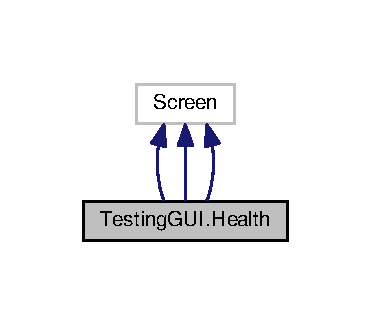
\includegraphics[width=178pt]{classTestingGUI_1_1Health__inherit__graph}
\end{center}
\end{figure}


Collaboration diagram for Testing\+G\+U\+I.\+Health\+:\nopagebreak
\begin{figure}[H]
\begin{center}
\leavevmode
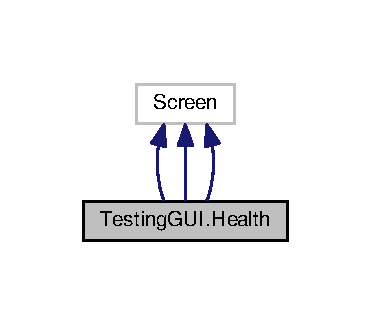
\includegraphics[width=178pt]{classTestingGUI_1_1Health__coll__graph}
\end{center}
\end{figure}
\subsection*{Public Member Functions}
\begin{DoxyCompactItemize}
\item 
def \hyperlink{classTestingGUI_1_1Health_acf40a31363f46003573ea00664734fc3}{\+\_\+\+\_\+init\+\_\+\+\_\+} (self, kwargs)
\item 
def \hyperlink{classTestingGUI_1_1Health_aa382e2bc40e918613d90dbd819974420}{check\+\_\+status\+\_\+\+A\+LL} (self)
\item 
def \hyperlink{classTestingGUI_1_1Health_a236b797764a726c3fe2d68f2fabaceb8}{grab\+\_\+name} (self, \hyperlink{classTestingGUI_1_1Health_a2c897cb32dd28d657ac3f22c64a14543}{ip})
\item 
def \hyperlink{classTestingGUI_1_1Health_ac36ce2de8d9aa5f3b687da2f836f0b3d}{health\+\_\+status} (self)
\item 
def \hyperlink{classTestingGUI_1_1Health_afde04eeef599765553cce6069cff429e}{retrieve\+Sensor} (self, ip\+\_\+addr, d)
\item 
def \hyperlink{classTestingGUI_1_1Health_ad38efcab164d7bbb4ec16c2086dc7760}{get\+Time} (self)
\item 
def \hyperlink{classTestingGUI_1_1Health_a3a6e2fca0c7a691527b14c79b388f6fd}{retrieve\+C\+R\+\_\+and\+\_\+status} (self, hour)
\item 
def \hyperlink{classTestingGUI_1_1Health_a1e3b9ff5f630c5f6d47bfefe26cfb39b}{clear\+\_\+selection} (self)
\item 
def \hyperlink{classTestingGUI_1_1Health_a06c77fae7dd08337985a3420a2cdbc81}{status\+\_\+popup} (self)
\item 
def \hyperlink{classTestingGUI_1_1Health_a73ccf83145b4adf9452f85a061c23dc9}{write\+\_\+} (self, ip\+\_\+addr)
\item 
def \hyperlink{classTestingGUI_1_1Health_acf40a31363f46003573ea00664734fc3}{\+\_\+\+\_\+init\+\_\+\+\_\+} (self, kwargs)
\item 
def \hyperlink{classTestingGUI_1_1Health_aa382e2bc40e918613d90dbd819974420}{check\+\_\+status\+\_\+\+A\+LL} (self)
\item 
def \hyperlink{classTestingGUI_1_1Health_a236b797764a726c3fe2d68f2fabaceb8}{grab\+\_\+name} (self, \hyperlink{classTestingGUI_1_1Health_a2c897cb32dd28d657ac3f22c64a14543}{ip})
\item 
def \hyperlink{classTestingGUI_1_1Health_ac36ce2de8d9aa5f3b687da2f836f0b3d}{health\+\_\+status} (self)
\item 
def \hyperlink{classTestingGUI_1_1Health_afde04eeef599765553cce6069cff429e}{retrieve\+Sensor} (self, ip\+\_\+addr, d)
\item 
def \hyperlink{classTestingGUI_1_1Health_ad38efcab164d7bbb4ec16c2086dc7760}{get\+Time} (self)
\item 
def \hyperlink{classTestingGUI_1_1Health_a3a6e2fca0c7a691527b14c79b388f6fd}{retrieve\+C\+R\+\_\+and\+\_\+status} (self, hour)
\item 
def \hyperlink{classTestingGUI_1_1Health_a1e3b9ff5f630c5f6d47bfefe26cfb39b}{clear\+\_\+selection} (self)
\item 
def \hyperlink{classTestingGUI_1_1Health_a06c77fae7dd08337985a3420a2cdbc81}{status\+\_\+popup} (self)
\item 
def \hyperlink{classTestingGUI_1_1Health_a73ccf83145b4adf9452f85a061c23dc9}{write\+\_\+} (self, ip\+\_\+addr)
\end{DoxyCompactItemize}
\subsection*{Static Public Attributes}
\begin{DoxyCompactItemize}
\item 
\hyperlink{classTestingGUI_1_1Health_a54e3f1adc11ad4d864b67012799706ac}{time} = String\+Property()
\item 
\hyperlink{classTestingGUI_1_1Health_aee1b4c1a46cdfd0438b155f1140ff72d}{date} = String\+Property()
\item 
\hyperlink{classTestingGUI_1_1Health_a93a88b008db790ac7cd19eb6b57c9031}{red} = String\+Property()
\item 
\hyperlink{classTestingGUI_1_1Health_ab7ae627cc3329ee7878f6d7e51ce548b}{green} = String\+Property()
\item 
\hyperlink{classTestingGUI_1_1Health_ab2d4c90c7dfd3dd5d2520ef3623aa1ad}{blue} = String\+Property()
\item 
\hyperlink{classTestingGUI_1_1Health_a995f5ac30531187402cb541794a95ada}{intensity} = String\+Property()
\item 
\hyperlink{classTestingGUI_1_1Health_ab0a961f891da2e855ac40338fa5cd40d}{status} = String\+Property()
\item 
\hyperlink{classTestingGUI_1_1Health_a129f267b2d7ad4d1aafc6253de5fdbdc}{light\+\_\+name} = String\+Property()
\item 
\hyperlink{classTestingGUI_1_1Health_a2c897cb32dd28d657ac3f22c64a14543}{ip} = String\+Property()
\item 
\hyperlink{classTestingGUI_1_1Health_ae6c66105b09f6d4c5722c0b681b5ed90}{sa} = String\+Property()
\item 
\hyperlink{classTestingGUI_1_1Health_af6181cd5d8046197aed006d3e3551ae0}{sr} = String\+Property()
\item 
\hyperlink{classTestingGUI_1_1Health_a75c173389aca62526762c23fd2b727fa}{sg} = String\+Property()
\item 
\hyperlink{classTestingGUI_1_1Health_a9f5fc022d375699c318a57d0819cfab4}{sb} = String\+Property()
\item 
\hyperlink{classTestingGUI_1_1Health_ae5f317f38e46fd38e0bce5f9a4c298e1}{A} = Numeric\+Property()
\item 
\hyperlink{classTestingGUI_1_1Health_a5677345190538551e2bb8fc754538b2b}{B} = Numeric\+Property()
\item 
\hyperlink{classTestingGUI_1_1Health_a90a59e432ad2eaae5d54691e4c020983}{R} = Numeric\+Property()
\item 
\hyperlink{classTestingGUI_1_1Health_a0a9e42ecd3551c7ea2f0bf31b5492a78}{G} = Numeric\+Property()
\end{DoxyCompactItemize}


\subsection{Constructor \& Destructor Documentation}
\index{Testing\+G\+U\+I\+::\+Health@{Testing\+G\+U\+I\+::\+Health}!\+\_\+\+\_\+init\+\_\+\+\_\+@{\+\_\+\+\_\+init\+\_\+\+\_\+}}
\index{\+\_\+\+\_\+init\+\_\+\+\_\+@{\+\_\+\+\_\+init\+\_\+\+\_\+}!Testing\+G\+U\+I\+::\+Health@{Testing\+G\+U\+I\+::\+Health}}
\subsubsection[{\texorpdfstring{\+\_\+\+\_\+init\+\_\+\+\_\+(self, kwargs)}{__init__(self, kwargs)}}]{\setlength{\rightskip}{0pt plus 5cm}def Testing\+G\+U\+I.\+Health.\+\_\+\+\_\+init\+\_\+\+\_\+ (
\begin{DoxyParamCaption}
\item[{}]{self, }
\item[{}]{kwargs}
\end{DoxyParamCaption}
)}\hypertarget{classTestingGUI_1_1Health_acf40a31363f46003573ea00664734fc3}{}\label{classTestingGUI_1_1Health_acf40a31363f46003573ea00664734fc3}
\index{Testing\+G\+U\+I\+::\+Health@{Testing\+G\+U\+I\+::\+Health}!\+\_\+\+\_\+init\+\_\+\+\_\+@{\+\_\+\+\_\+init\+\_\+\+\_\+}}
\index{\+\_\+\+\_\+init\+\_\+\+\_\+@{\+\_\+\+\_\+init\+\_\+\+\_\+}!Testing\+G\+U\+I\+::\+Health@{Testing\+G\+U\+I\+::\+Health}}
\subsubsection[{\texorpdfstring{\+\_\+\+\_\+init\+\_\+\+\_\+(self, kwargs)}{__init__(self, kwargs)}}]{\setlength{\rightskip}{0pt plus 5cm}def Testing\+G\+U\+I.\+Health.\+\_\+\+\_\+init\+\_\+\+\_\+ (
\begin{DoxyParamCaption}
\item[{}]{self, }
\item[{}]{kwargs}
\end{DoxyParamCaption}
)}\hypertarget{classTestingGUI_1_1Health_acf40a31363f46003573ea00664734fc3}{}\label{classTestingGUI_1_1Health_acf40a31363f46003573ea00664734fc3}


\subsection{Member Function Documentation}
\index{Testing\+G\+U\+I\+::\+Health@{Testing\+G\+U\+I\+::\+Health}!check\+\_\+status\+\_\+\+A\+LL@{check\+\_\+status\+\_\+\+A\+LL}}
\index{check\+\_\+status\+\_\+\+A\+LL@{check\+\_\+status\+\_\+\+A\+LL}!Testing\+G\+U\+I\+::\+Health@{Testing\+G\+U\+I\+::\+Health}}
\subsubsection[{\texorpdfstring{check\+\_\+status\+\_\+\+A\+L\+L(self)}{check_status_ALL(self)}}]{\setlength{\rightskip}{0pt plus 5cm}def Testing\+G\+U\+I.\+Health.\+check\+\_\+status\+\_\+\+A\+LL (
\begin{DoxyParamCaption}
\item[{}]{self}
\end{DoxyParamCaption}
)}\hypertarget{classTestingGUI_1_1Health_aa382e2bc40e918613d90dbd819974420}{}\label{classTestingGUI_1_1Health_aa382e2bc40e918613d90dbd819974420}
\index{Testing\+G\+U\+I\+::\+Health@{Testing\+G\+U\+I\+::\+Health}!check\+\_\+status\+\_\+\+A\+LL@{check\+\_\+status\+\_\+\+A\+LL}}
\index{check\+\_\+status\+\_\+\+A\+LL@{check\+\_\+status\+\_\+\+A\+LL}!Testing\+G\+U\+I\+::\+Health@{Testing\+G\+U\+I\+::\+Health}}
\subsubsection[{\texorpdfstring{check\+\_\+status\+\_\+\+A\+L\+L(self)}{check_status_ALL(self)}}]{\setlength{\rightskip}{0pt plus 5cm}def Testing\+G\+U\+I.\+Health.\+check\+\_\+status\+\_\+\+A\+LL (
\begin{DoxyParamCaption}
\item[{}]{self}
\end{DoxyParamCaption}
)}\hypertarget{classTestingGUI_1_1Health_aa382e2bc40e918613d90dbd819974420}{}\label{classTestingGUI_1_1Health_aa382e2bc40e918613d90dbd819974420}
\index{Testing\+G\+U\+I\+::\+Health@{Testing\+G\+U\+I\+::\+Health}!clear\+\_\+selection@{clear\+\_\+selection}}
\index{clear\+\_\+selection@{clear\+\_\+selection}!Testing\+G\+U\+I\+::\+Health@{Testing\+G\+U\+I\+::\+Health}}
\subsubsection[{\texorpdfstring{clear\+\_\+selection(self)}{clear_selection(self)}}]{\setlength{\rightskip}{0pt plus 5cm}def Testing\+G\+U\+I.\+Health.\+clear\+\_\+selection (
\begin{DoxyParamCaption}
\item[{}]{self}
\end{DoxyParamCaption}
)}\hypertarget{classTestingGUI_1_1Health_a1e3b9ff5f630c5f6d47bfefe26cfb39b}{}\label{classTestingGUI_1_1Health_a1e3b9ff5f630c5f6d47bfefe26cfb39b}
\index{Testing\+G\+U\+I\+::\+Health@{Testing\+G\+U\+I\+::\+Health}!clear\+\_\+selection@{clear\+\_\+selection}}
\index{clear\+\_\+selection@{clear\+\_\+selection}!Testing\+G\+U\+I\+::\+Health@{Testing\+G\+U\+I\+::\+Health}}
\subsubsection[{\texorpdfstring{clear\+\_\+selection(self)}{clear_selection(self)}}]{\setlength{\rightskip}{0pt plus 5cm}def Testing\+G\+U\+I.\+Health.\+clear\+\_\+selection (
\begin{DoxyParamCaption}
\item[{}]{self}
\end{DoxyParamCaption}
)}\hypertarget{classTestingGUI_1_1Health_a1e3b9ff5f630c5f6d47bfefe26cfb39b}{}\label{classTestingGUI_1_1Health_a1e3b9ff5f630c5f6d47bfefe26cfb39b}
\index{Testing\+G\+U\+I\+::\+Health@{Testing\+G\+U\+I\+::\+Health}!get\+Time@{get\+Time}}
\index{get\+Time@{get\+Time}!Testing\+G\+U\+I\+::\+Health@{Testing\+G\+U\+I\+::\+Health}}
\subsubsection[{\texorpdfstring{get\+Time(self)}{getTime(self)}}]{\setlength{\rightskip}{0pt plus 5cm}def Testing\+G\+U\+I.\+Health.\+get\+Time (
\begin{DoxyParamCaption}
\item[{}]{self}
\end{DoxyParamCaption}
)}\hypertarget{classTestingGUI_1_1Health_ad38efcab164d7bbb4ec16c2086dc7760}{}\label{classTestingGUI_1_1Health_ad38efcab164d7bbb4ec16c2086dc7760}
\index{Testing\+G\+U\+I\+::\+Health@{Testing\+G\+U\+I\+::\+Health}!get\+Time@{get\+Time}}
\index{get\+Time@{get\+Time}!Testing\+G\+U\+I\+::\+Health@{Testing\+G\+U\+I\+::\+Health}}
\subsubsection[{\texorpdfstring{get\+Time(self)}{getTime(self)}}]{\setlength{\rightskip}{0pt plus 5cm}def Testing\+G\+U\+I.\+Health.\+get\+Time (
\begin{DoxyParamCaption}
\item[{}]{self}
\end{DoxyParamCaption}
)}\hypertarget{classTestingGUI_1_1Health_ad38efcab164d7bbb4ec16c2086dc7760}{}\label{classTestingGUI_1_1Health_ad38efcab164d7bbb4ec16c2086dc7760}
\index{Testing\+G\+U\+I\+::\+Health@{Testing\+G\+U\+I\+::\+Health}!grab\+\_\+name@{grab\+\_\+name}}
\index{grab\+\_\+name@{grab\+\_\+name}!Testing\+G\+U\+I\+::\+Health@{Testing\+G\+U\+I\+::\+Health}}
\subsubsection[{\texorpdfstring{grab\+\_\+name(self, ip)}{grab_name(self, ip)}}]{\setlength{\rightskip}{0pt plus 5cm}def Testing\+G\+U\+I.\+Health.\+grab\+\_\+name (
\begin{DoxyParamCaption}
\item[{}]{self, }
\item[{}]{ip}
\end{DoxyParamCaption}
)}\hypertarget{classTestingGUI_1_1Health_a236b797764a726c3fe2d68f2fabaceb8}{}\label{classTestingGUI_1_1Health_a236b797764a726c3fe2d68f2fabaceb8}
\index{Testing\+G\+U\+I\+::\+Health@{Testing\+G\+U\+I\+::\+Health}!grab\+\_\+name@{grab\+\_\+name}}
\index{grab\+\_\+name@{grab\+\_\+name}!Testing\+G\+U\+I\+::\+Health@{Testing\+G\+U\+I\+::\+Health}}
\subsubsection[{\texorpdfstring{grab\+\_\+name(self, ip)}{grab_name(self, ip)}}]{\setlength{\rightskip}{0pt plus 5cm}def Testing\+G\+U\+I.\+Health.\+grab\+\_\+name (
\begin{DoxyParamCaption}
\item[{}]{self, }
\item[{}]{ip}
\end{DoxyParamCaption}
)}\hypertarget{classTestingGUI_1_1Health_a236b797764a726c3fe2d68f2fabaceb8}{}\label{classTestingGUI_1_1Health_a236b797764a726c3fe2d68f2fabaceb8}
\index{Testing\+G\+U\+I\+::\+Health@{Testing\+G\+U\+I\+::\+Health}!health\+\_\+status@{health\+\_\+status}}
\index{health\+\_\+status@{health\+\_\+status}!Testing\+G\+U\+I\+::\+Health@{Testing\+G\+U\+I\+::\+Health}}
\subsubsection[{\texorpdfstring{health\+\_\+status(self)}{health_status(self)}}]{\setlength{\rightskip}{0pt plus 5cm}def Testing\+G\+U\+I.\+Health.\+health\+\_\+status (
\begin{DoxyParamCaption}
\item[{}]{self}
\end{DoxyParamCaption}
)}\hypertarget{classTestingGUI_1_1Health_ac36ce2de8d9aa5f3b687da2f836f0b3d}{}\label{classTestingGUI_1_1Health_ac36ce2de8d9aa5f3b687da2f836f0b3d}
\index{Testing\+G\+U\+I\+::\+Health@{Testing\+G\+U\+I\+::\+Health}!health\+\_\+status@{health\+\_\+status}}
\index{health\+\_\+status@{health\+\_\+status}!Testing\+G\+U\+I\+::\+Health@{Testing\+G\+U\+I\+::\+Health}}
\subsubsection[{\texorpdfstring{health\+\_\+status(self)}{health_status(self)}}]{\setlength{\rightskip}{0pt plus 5cm}def Testing\+G\+U\+I.\+Health.\+health\+\_\+status (
\begin{DoxyParamCaption}
\item[{}]{self}
\end{DoxyParamCaption}
)}\hypertarget{classTestingGUI_1_1Health_ac36ce2de8d9aa5f3b687da2f836f0b3d}{}\label{classTestingGUI_1_1Health_ac36ce2de8d9aa5f3b687da2f836f0b3d}
\index{Testing\+G\+U\+I\+::\+Health@{Testing\+G\+U\+I\+::\+Health}!retrieve\+C\+R\+\_\+and\+\_\+status@{retrieve\+C\+R\+\_\+and\+\_\+status}}
\index{retrieve\+C\+R\+\_\+and\+\_\+status@{retrieve\+C\+R\+\_\+and\+\_\+status}!Testing\+G\+U\+I\+::\+Health@{Testing\+G\+U\+I\+::\+Health}}
\subsubsection[{\texorpdfstring{retrieve\+C\+R\+\_\+and\+\_\+status(self, hour)}{retrieveCR_and_status(self, hour)}}]{\setlength{\rightskip}{0pt plus 5cm}def Testing\+G\+U\+I.\+Health.\+retrieve\+C\+R\+\_\+and\+\_\+status (
\begin{DoxyParamCaption}
\item[{}]{self, }
\item[{}]{hour}
\end{DoxyParamCaption}
)}\hypertarget{classTestingGUI_1_1Health_a3a6e2fca0c7a691527b14c79b388f6fd}{}\label{classTestingGUI_1_1Health_a3a6e2fca0c7a691527b14c79b388f6fd}
\index{Testing\+G\+U\+I\+::\+Health@{Testing\+G\+U\+I\+::\+Health}!retrieve\+C\+R\+\_\+and\+\_\+status@{retrieve\+C\+R\+\_\+and\+\_\+status}}
\index{retrieve\+C\+R\+\_\+and\+\_\+status@{retrieve\+C\+R\+\_\+and\+\_\+status}!Testing\+G\+U\+I\+::\+Health@{Testing\+G\+U\+I\+::\+Health}}
\subsubsection[{\texorpdfstring{retrieve\+C\+R\+\_\+and\+\_\+status(self, hour)}{retrieveCR_and_status(self, hour)}}]{\setlength{\rightskip}{0pt plus 5cm}def Testing\+G\+U\+I.\+Health.\+retrieve\+C\+R\+\_\+and\+\_\+status (
\begin{DoxyParamCaption}
\item[{}]{self, }
\item[{}]{hour}
\end{DoxyParamCaption}
)}\hypertarget{classTestingGUI_1_1Health_a3a6e2fca0c7a691527b14c79b388f6fd}{}\label{classTestingGUI_1_1Health_a3a6e2fca0c7a691527b14c79b388f6fd}
\index{Testing\+G\+U\+I\+::\+Health@{Testing\+G\+U\+I\+::\+Health}!retrieve\+Sensor@{retrieve\+Sensor}}
\index{retrieve\+Sensor@{retrieve\+Sensor}!Testing\+G\+U\+I\+::\+Health@{Testing\+G\+U\+I\+::\+Health}}
\subsubsection[{\texorpdfstring{retrieve\+Sensor(self, ip\+\_\+addr, d)}{retrieveSensor(self, ip_addr, d)}}]{\setlength{\rightskip}{0pt plus 5cm}def Testing\+G\+U\+I.\+Health.\+retrieve\+Sensor (
\begin{DoxyParamCaption}
\item[{}]{self, }
\item[{}]{ip\+\_\+addr, }
\item[{}]{d}
\end{DoxyParamCaption}
)}\hypertarget{classTestingGUI_1_1Health_afde04eeef599765553cce6069cff429e}{}\label{classTestingGUI_1_1Health_afde04eeef599765553cce6069cff429e}
\index{Testing\+G\+U\+I\+::\+Health@{Testing\+G\+U\+I\+::\+Health}!retrieve\+Sensor@{retrieve\+Sensor}}
\index{retrieve\+Sensor@{retrieve\+Sensor}!Testing\+G\+U\+I\+::\+Health@{Testing\+G\+U\+I\+::\+Health}}
\subsubsection[{\texorpdfstring{retrieve\+Sensor(self, ip\+\_\+addr, d)}{retrieveSensor(self, ip_addr, d)}}]{\setlength{\rightskip}{0pt plus 5cm}def Testing\+G\+U\+I.\+Health.\+retrieve\+Sensor (
\begin{DoxyParamCaption}
\item[{}]{self, }
\item[{}]{ip\+\_\+addr, }
\item[{}]{d}
\end{DoxyParamCaption}
)}\hypertarget{classTestingGUI_1_1Health_afde04eeef599765553cce6069cff429e}{}\label{classTestingGUI_1_1Health_afde04eeef599765553cce6069cff429e}
\index{Testing\+G\+U\+I\+::\+Health@{Testing\+G\+U\+I\+::\+Health}!status\+\_\+popup@{status\+\_\+popup}}
\index{status\+\_\+popup@{status\+\_\+popup}!Testing\+G\+U\+I\+::\+Health@{Testing\+G\+U\+I\+::\+Health}}
\subsubsection[{\texorpdfstring{status\+\_\+popup(self)}{status_popup(self)}}]{\setlength{\rightskip}{0pt plus 5cm}def Testing\+G\+U\+I.\+Health.\+status\+\_\+popup (
\begin{DoxyParamCaption}
\item[{}]{self}
\end{DoxyParamCaption}
)}\hypertarget{classTestingGUI_1_1Health_a06c77fae7dd08337985a3420a2cdbc81}{}\label{classTestingGUI_1_1Health_a06c77fae7dd08337985a3420a2cdbc81}
\index{Testing\+G\+U\+I\+::\+Health@{Testing\+G\+U\+I\+::\+Health}!status\+\_\+popup@{status\+\_\+popup}}
\index{status\+\_\+popup@{status\+\_\+popup}!Testing\+G\+U\+I\+::\+Health@{Testing\+G\+U\+I\+::\+Health}}
\subsubsection[{\texorpdfstring{status\+\_\+popup(self)}{status_popup(self)}}]{\setlength{\rightskip}{0pt plus 5cm}def Testing\+G\+U\+I.\+Health.\+status\+\_\+popup (
\begin{DoxyParamCaption}
\item[{}]{self}
\end{DoxyParamCaption}
)}\hypertarget{classTestingGUI_1_1Health_a06c77fae7dd08337985a3420a2cdbc81}{}\label{classTestingGUI_1_1Health_a06c77fae7dd08337985a3420a2cdbc81}
\index{Testing\+G\+U\+I\+::\+Health@{Testing\+G\+U\+I\+::\+Health}!write\+\_\+@{write\+\_\+}}
\index{write\+\_\+@{write\+\_\+}!Testing\+G\+U\+I\+::\+Health@{Testing\+G\+U\+I\+::\+Health}}
\subsubsection[{\texorpdfstring{write\+\_\+(self, ip\+\_\+addr)}{write_(self, ip_addr)}}]{\setlength{\rightskip}{0pt plus 5cm}def Testing\+G\+U\+I.\+Health.\+write\+\_\+ (
\begin{DoxyParamCaption}
\item[{}]{self, }
\item[{}]{ip\+\_\+addr}
\end{DoxyParamCaption}
)}\hypertarget{classTestingGUI_1_1Health_a73ccf83145b4adf9452f85a061c23dc9}{}\label{classTestingGUI_1_1Health_a73ccf83145b4adf9452f85a061c23dc9}
\index{Testing\+G\+U\+I\+::\+Health@{Testing\+G\+U\+I\+::\+Health}!write\+\_\+@{write\+\_\+}}
\index{write\+\_\+@{write\+\_\+}!Testing\+G\+U\+I\+::\+Health@{Testing\+G\+U\+I\+::\+Health}}
\subsubsection[{\texorpdfstring{write\+\_\+(self, ip\+\_\+addr)}{write_(self, ip_addr)}}]{\setlength{\rightskip}{0pt plus 5cm}def Testing\+G\+U\+I.\+Health.\+write\+\_\+ (
\begin{DoxyParamCaption}
\item[{}]{self, }
\item[{}]{ip\+\_\+addr}
\end{DoxyParamCaption}
)}\hypertarget{classTestingGUI_1_1Health_a73ccf83145b4adf9452f85a061c23dc9}{}\label{classTestingGUI_1_1Health_a73ccf83145b4adf9452f85a061c23dc9}


\subsection{Member Data Documentation}
\index{Testing\+G\+U\+I\+::\+Health@{Testing\+G\+U\+I\+::\+Health}!A@{A}}
\index{A@{A}!Testing\+G\+U\+I\+::\+Health@{Testing\+G\+U\+I\+::\+Health}}
\subsubsection[{\texorpdfstring{A}{A}}]{\setlength{\rightskip}{0pt plus 5cm}Testing\+G\+U\+I.\+Health.\+A = Numeric\+Property()\hspace{0.3cm}{\ttfamily [static]}}\hypertarget{classTestingGUI_1_1Health_ae5f317f38e46fd38e0bce5f9a4c298e1}{}\label{classTestingGUI_1_1Health_ae5f317f38e46fd38e0bce5f9a4c298e1}
\index{Testing\+G\+U\+I\+::\+Health@{Testing\+G\+U\+I\+::\+Health}!B@{B}}
\index{B@{B}!Testing\+G\+U\+I\+::\+Health@{Testing\+G\+U\+I\+::\+Health}}
\subsubsection[{\texorpdfstring{B}{B}}]{\setlength{\rightskip}{0pt plus 5cm}Testing\+G\+U\+I.\+Health.\+B = Numeric\+Property()\hspace{0.3cm}{\ttfamily [static]}}\hypertarget{classTestingGUI_1_1Health_a5677345190538551e2bb8fc754538b2b}{}\label{classTestingGUI_1_1Health_a5677345190538551e2bb8fc754538b2b}
\index{Testing\+G\+U\+I\+::\+Health@{Testing\+G\+U\+I\+::\+Health}!blue@{blue}}
\index{blue@{blue}!Testing\+G\+U\+I\+::\+Health@{Testing\+G\+U\+I\+::\+Health}}
\subsubsection[{\texorpdfstring{blue}{blue}}]{\setlength{\rightskip}{0pt plus 5cm}Testing\+G\+U\+I.\+Health.\+blue = String\+Property()\hspace{0.3cm}{\ttfamily [static]}}\hypertarget{classTestingGUI_1_1Health_ab2d4c90c7dfd3dd5d2520ef3623aa1ad}{}\label{classTestingGUI_1_1Health_ab2d4c90c7dfd3dd5d2520ef3623aa1ad}
\index{Testing\+G\+U\+I\+::\+Health@{Testing\+G\+U\+I\+::\+Health}!date@{date}}
\index{date@{date}!Testing\+G\+U\+I\+::\+Health@{Testing\+G\+U\+I\+::\+Health}}
\subsubsection[{\texorpdfstring{date}{date}}]{\setlength{\rightskip}{0pt plus 5cm}Testing\+G\+U\+I.\+Health.\+date = String\+Property()\hspace{0.3cm}{\ttfamily [static]}}\hypertarget{classTestingGUI_1_1Health_aee1b4c1a46cdfd0438b155f1140ff72d}{}\label{classTestingGUI_1_1Health_aee1b4c1a46cdfd0438b155f1140ff72d}
\index{Testing\+G\+U\+I\+::\+Health@{Testing\+G\+U\+I\+::\+Health}!G@{G}}
\index{G@{G}!Testing\+G\+U\+I\+::\+Health@{Testing\+G\+U\+I\+::\+Health}}
\subsubsection[{\texorpdfstring{G}{G}}]{\setlength{\rightskip}{0pt plus 5cm}Testing\+G\+U\+I.\+Health.\+G = Numeric\+Property()\hspace{0.3cm}{\ttfamily [static]}}\hypertarget{classTestingGUI_1_1Health_a0a9e42ecd3551c7ea2f0bf31b5492a78}{}\label{classTestingGUI_1_1Health_a0a9e42ecd3551c7ea2f0bf31b5492a78}
\index{Testing\+G\+U\+I\+::\+Health@{Testing\+G\+U\+I\+::\+Health}!green@{green}}
\index{green@{green}!Testing\+G\+U\+I\+::\+Health@{Testing\+G\+U\+I\+::\+Health}}
\subsubsection[{\texorpdfstring{green}{green}}]{\setlength{\rightskip}{0pt plus 5cm}Testing\+G\+U\+I.\+Health.\+green = String\+Property()\hspace{0.3cm}{\ttfamily [static]}}\hypertarget{classTestingGUI_1_1Health_ab7ae627cc3329ee7878f6d7e51ce548b}{}\label{classTestingGUI_1_1Health_ab7ae627cc3329ee7878f6d7e51ce548b}
\index{Testing\+G\+U\+I\+::\+Health@{Testing\+G\+U\+I\+::\+Health}!intensity@{intensity}}
\index{intensity@{intensity}!Testing\+G\+U\+I\+::\+Health@{Testing\+G\+U\+I\+::\+Health}}
\subsubsection[{\texorpdfstring{intensity}{intensity}}]{\setlength{\rightskip}{0pt plus 5cm}Testing\+G\+U\+I.\+Health.\+intensity = String\+Property()\hspace{0.3cm}{\ttfamily [static]}}\hypertarget{classTestingGUI_1_1Health_a995f5ac30531187402cb541794a95ada}{}\label{classTestingGUI_1_1Health_a995f5ac30531187402cb541794a95ada}
\index{Testing\+G\+U\+I\+::\+Health@{Testing\+G\+U\+I\+::\+Health}!ip@{ip}}
\index{ip@{ip}!Testing\+G\+U\+I\+::\+Health@{Testing\+G\+U\+I\+::\+Health}}
\subsubsection[{\texorpdfstring{ip}{ip}}]{\setlength{\rightskip}{0pt plus 5cm}Testing\+G\+U\+I.\+Health.\+ip = String\+Property()\hspace{0.3cm}{\ttfamily [static]}}\hypertarget{classTestingGUI_1_1Health_a2c897cb32dd28d657ac3f22c64a14543}{}\label{classTestingGUI_1_1Health_a2c897cb32dd28d657ac3f22c64a14543}
\index{Testing\+G\+U\+I\+::\+Health@{Testing\+G\+U\+I\+::\+Health}!light\+\_\+name@{light\+\_\+name}}
\index{light\+\_\+name@{light\+\_\+name}!Testing\+G\+U\+I\+::\+Health@{Testing\+G\+U\+I\+::\+Health}}
\subsubsection[{\texorpdfstring{light\+\_\+name}{light_name}}]{\setlength{\rightskip}{0pt plus 5cm}Testing\+G\+U\+I.\+Health.\+light\+\_\+name = String\+Property()\hspace{0.3cm}{\ttfamily [static]}}\hypertarget{classTestingGUI_1_1Health_a129f267b2d7ad4d1aafc6253de5fdbdc}{}\label{classTestingGUI_1_1Health_a129f267b2d7ad4d1aafc6253de5fdbdc}
\index{Testing\+G\+U\+I\+::\+Health@{Testing\+G\+U\+I\+::\+Health}!R@{R}}
\index{R@{R}!Testing\+G\+U\+I\+::\+Health@{Testing\+G\+U\+I\+::\+Health}}
\subsubsection[{\texorpdfstring{R}{R}}]{\setlength{\rightskip}{0pt plus 5cm}Testing\+G\+U\+I.\+Health.\+R = Numeric\+Property()\hspace{0.3cm}{\ttfamily [static]}}\hypertarget{classTestingGUI_1_1Health_a90a59e432ad2eaae5d54691e4c020983}{}\label{classTestingGUI_1_1Health_a90a59e432ad2eaae5d54691e4c020983}
\index{Testing\+G\+U\+I\+::\+Health@{Testing\+G\+U\+I\+::\+Health}!red@{red}}
\index{red@{red}!Testing\+G\+U\+I\+::\+Health@{Testing\+G\+U\+I\+::\+Health}}
\subsubsection[{\texorpdfstring{red}{red}}]{\setlength{\rightskip}{0pt plus 5cm}Testing\+G\+U\+I.\+Health.\+red = String\+Property()\hspace{0.3cm}{\ttfamily [static]}}\hypertarget{classTestingGUI_1_1Health_a93a88b008db790ac7cd19eb6b57c9031}{}\label{classTestingGUI_1_1Health_a93a88b008db790ac7cd19eb6b57c9031}
\index{Testing\+G\+U\+I\+::\+Health@{Testing\+G\+U\+I\+::\+Health}!sa@{sa}}
\index{sa@{sa}!Testing\+G\+U\+I\+::\+Health@{Testing\+G\+U\+I\+::\+Health}}
\subsubsection[{\texorpdfstring{sa}{sa}}]{\setlength{\rightskip}{0pt plus 5cm}Testing\+G\+U\+I.\+Health.\+sa = String\+Property()\hspace{0.3cm}{\ttfamily [static]}}\hypertarget{classTestingGUI_1_1Health_ae6c66105b09f6d4c5722c0b681b5ed90}{}\label{classTestingGUI_1_1Health_ae6c66105b09f6d4c5722c0b681b5ed90}
\index{Testing\+G\+U\+I\+::\+Health@{Testing\+G\+U\+I\+::\+Health}!sb@{sb}}
\index{sb@{sb}!Testing\+G\+U\+I\+::\+Health@{Testing\+G\+U\+I\+::\+Health}}
\subsubsection[{\texorpdfstring{sb}{sb}}]{\setlength{\rightskip}{0pt plus 5cm}Testing\+G\+U\+I.\+Health.\+sb = String\+Property()\hspace{0.3cm}{\ttfamily [static]}}\hypertarget{classTestingGUI_1_1Health_a9f5fc022d375699c318a57d0819cfab4}{}\label{classTestingGUI_1_1Health_a9f5fc022d375699c318a57d0819cfab4}
\index{Testing\+G\+U\+I\+::\+Health@{Testing\+G\+U\+I\+::\+Health}!sg@{sg}}
\index{sg@{sg}!Testing\+G\+U\+I\+::\+Health@{Testing\+G\+U\+I\+::\+Health}}
\subsubsection[{\texorpdfstring{sg}{sg}}]{\setlength{\rightskip}{0pt plus 5cm}Testing\+G\+U\+I.\+Health.\+sg = String\+Property()\hspace{0.3cm}{\ttfamily [static]}}\hypertarget{classTestingGUI_1_1Health_a75c173389aca62526762c23fd2b727fa}{}\label{classTestingGUI_1_1Health_a75c173389aca62526762c23fd2b727fa}
\index{Testing\+G\+U\+I\+::\+Health@{Testing\+G\+U\+I\+::\+Health}!sr@{sr}}
\index{sr@{sr}!Testing\+G\+U\+I\+::\+Health@{Testing\+G\+U\+I\+::\+Health}}
\subsubsection[{\texorpdfstring{sr}{sr}}]{\setlength{\rightskip}{0pt plus 5cm}Testing\+G\+U\+I.\+Health.\+sr = String\+Property()\hspace{0.3cm}{\ttfamily [static]}}\hypertarget{classTestingGUI_1_1Health_af6181cd5d8046197aed006d3e3551ae0}{}\label{classTestingGUI_1_1Health_af6181cd5d8046197aed006d3e3551ae0}
\index{Testing\+G\+U\+I\+::\+Health@{Testing\+G\+U\+I\+::\+Health}!status@{status}}
\index{status@{status}!Testing\+G\+U\+I\+::\+Health@{Testing\+G\+U\+I\+::\+Health}}
\subsubsection[{\texorpdfstring{status}{status}}]{\setlength{\rightskip}{0pt plus 5cm}Testing\+G\+U\+I.\+Health.\+status = String\+Property()\hspace{0.3cm}{\ttfamily [static]}}\hypertarget{classTestingGUI_1_1Health_ab0a961f891da2e855ac40338fa5cd40d}{}\label{classTestingGUI_1_1Health_ab0a961f891da2e855ac40338fa5cd40d}
\index{Testing\+G\+U\+I\+::\+Health@{Testing\+G\+U\+I\+::\+Health}!time@{time}}
\index{time@{time}!Testing\+G\+U\+I\+::\+Health@{Testing\+G\+U\+I\+::\+Health}}
\subsubsection[{\texorpdfstring{time}{time}}]{\setlength{\rightskip}{0pt plus 5cm}Testing\+G\+U\+I.\+Health.\+time = String\+Property()\hspace{0.3cm}{\ttfamily [static]}}\hypertarget{classTestingGUI_1_1Health_a54e3f1adc11ad4d864b67012799706ac}{}\label{classTestingGUI_1_1Health_a54e3f1adc11ad4d864b67012799706ac}


The documentation for this class was generated from the following file\+:\begin{DoxyCompactItemize}
\item 
/home/jac0656/\+Desktop/\+J-\/\+O-\/\+R-\/\+G-\/\+E/\+U\+N\+T-\/\+N\+A\+S\+A/\+G\+U\+I/\hyperlink{GUI_2TestingGUI_8py}{Testing\+G\+U\+I.\+py}\end{DoxyCompactItemize}

\hypertarget{classGUI8_1_1Health}{}\section{G\+U\+I8.\+Health Class Reference}
\label{classGUI8_1_1Health}\index{G\+U\+I8.\+Health@{G\+U\+I8.\+Health}}


Inheritance diagram for G\+U\+I8.\+Health\+:
\nopagebreak
\begin{figure}[H]
\begin{center}
\leavevmode
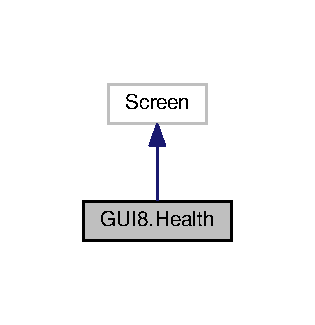
\includegraphics[width=151pt]{classGUI8_1_1Health__inherit__graph}
\end{center}
\end{figure}


Collaboration diagram for G\+U\+I8.\+Health\+:
\nopagebreak
\begin{figure}[H]
\begin{center}
\leavevmode
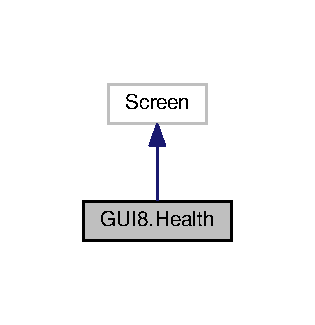
\includegraphics[width=151pt]{classGUI8_1_1Health__coll__graph}
\end{center}
\end{figure}
\subsection*{Public Member Functions}
\begin{DoxyCompactItemize}
\item 
def \hyperlink{classGUI8_1_1Health_aa7e6e19d9db87725774678615b135709}{\+\_\+\+\_\+init\+\_\+\+\_\+} (self, kwargs)
\item 
def \hyperlink{classGUI8_1_1Health_a42a643ea13a14c53bfc681856be2f216}{check\+\_\+status\+\_\+\+A\+LL} (self)
\item 
def \hyperlink{classGUI8_1_1Health_a3ad87b74336ede1a14ece2d7ef504f82}{health\+\_\+status} (self)
\item 
def \hyperlink{classGUI8_1_1Health_a740ea34528236064297a25d1cc94ec6f}{health\+\_\+popup} (self)
\item 
def \hyperlink{classGUI8_1_1Health_a8ba7d780a1de6dd72011ffcb7a03a10c}{back\+\_\+to\+\_\+rv} (self, arg1)
\item 
def \hyperlink{classGUI8_1_1Health_a4acd1eda551dc56bdc3880785c5bce64}{retrieve\+Sensor} (self, ip\+\_\+addr, d)
\item 
def \hyperlink{classGUI8_1_1Health_a26a2e1f462c6db875f4fb580ed5b573a}{get\+Time} (self)
\item 
def \hyperlink{classGUI8_1_1Health_aabe5e1b2073d1e70495f64a59420450a}{retrieve\+C\+R\+\_\+and\+\_\+status} (self, hour)
\item 
def \hyperlink{classGUI8_1_1Health_aa1cc0aedd0fe8d91556e0f0c15f1f48c}{clear\+\_\+selection} (self)
\item 
def \hyperlink{classGUI8_1_1Health_a8640059475dc70c6254bc06f13343c45}{status\+\_\+popup} (self)
\item 
def \hyperlink{classGUI8_1_1Health_aa7e6e19d9db87725774678615b135709}{\+\_\+\+\_\+init\+\_\+\+\_\+} (self, kwargs)
\item 
def \hyperlink{classGUI8_1_1Health_a42a643ea13a14c53bfc681856be2f216}{check\+\_\+status\+\_\+\+A\+LL} (self)
\item 
def \hyperlink{classGUI8_1_1Health_a3ad87b74336ede1a14ece2d7ef504f82}{health\+\_\+status} (self)
\item 
def \hyperlink{classGUI8_1_1Health_a740ea34528236064297a25d1cc94ec6f}{health\+\_\+popup} (self)
\item 
def \hyperlink{classGUI8_1_1Health_a8ba7d780a1de6dd72011ffcb7a03a10c}{back\+\_\+to\+\_\+rv} (self, arg1)
\item 
def \hyperlink{classGUI8_1_1Health_a4acd1eda551dc56bdc3880785c5bce64}{retrieve\+Sensor} (self, ip\+\_\+addr, d)
\item 
def \hyperlink{classGUI8_1_1Health_a26a2e1f462c6db875f4fb580ed5b573a}{get\+Time} (self)
\item 
def \hyperlink{classGUI8_1_1Health_aabe5e1b2073d1e70495f64a59420450a}{retrieve\+C\+R\+\_\+and\+\_\+status} (self, hour)
\item 
def \hyperlink{classGUI8_1_1Health_aa1cc0aedd0fe8d91556e0f0c15f1f48c}{clear\+\_\+selection} (self)
\item 
def \hyperlink{classGUI8_1_1Health_a8640059475dc70c6254bc06f13343c45}{status\+\_\+popup} (self)
\end{DoxyCompactItemize}
\subsection*{Static Public Attributes}
\begin{DoxyCompactItemize}
\item 
\hyperlink{classGUI8_1_1Health_a70f5dedaa1d04590be02c340943fa8e4}{time} = String\+Property()
\item 
\hyperlink{classGUI8_1_1Health_adf047d5dc696b47ed1d41693c1fe858d}{date} = String\+Property()
\item 
\hyperlink{classGUI8_1_1Health_a3ff74efb301f8299cf691751119e1b15}{red} = String\+Property()
\item 
\hyperlink{classGUI8_1_1Health_a83450a6d9466cb310e55f61c160698ec}{green} = String\+Property()
\item 
\hyperlink{classGUI8_1_1Health_a724902ae6c4a9e020cc46482e553c0a9}{blue} = String\+Property()
\item 
\hyperlink{classGUI8_1_1Health_a0a9778defbe25346655b8e1e4fa642a6}{intensity} = String\+Property()
\item 
\hyperlink{classGUI8_1_1Health_a51e3464840e9630763299d492a988b12}{status} = String\+Property()
\item 
\hyperlink{classGUI8_1_1Health_a06b3b36d8461b537d2d79daff690a91b}{light\+\_\+name} = String\+Property()
\item 
\hyperlink{classGUI8_1_1Health_a81147b4aa865492667f09581988cda72}{ip} = String\+Property()
\item 
\hyperlink{classGUI8_1_1Health_a635f4169a6bcffd7f58ca68d31bbcb6d}{sa} = String\+Property()
\item 
\hyperlink{classGUI8_1_1Health_a1c95aff816745a8727529768e6de6fdf}{sr} = String\+Property()
\item 
\hyperlink{classGUI8_1_1Health_a8d847a1f3db5ef07ae447de48eb27a7a}{sg} = String\+Property()
\item 
\hyperlink{classGUI8_1_1Health_a87f9894e10b5d33548480866ef2b82bd}{sb} = String\+Property()
\item 
\hyperlink{classGUI8_1_1Health_af494e21ab6ef3dee82770591aaaa163a}{A} = Numeric\+Property()
\item 
\hyperlink{classGUI8_1_1Health_a44e4660f74520f1d5b94467977f18f60}{B} = Numeric\+Property()
\item 
\hyperlink{classGUI8_1_1Health_a8da66dfab168d5bb42fce76eb1f4f371}{R} = Numeric\+Property()
\item 
\hyperlink{classGUI8_1_1Health_a49d19654302f8f806eefc20ebee054df}{G} = Numeric\+Property()
\end{DoxyCompactItemize}


\subsection{Constructor \& Destructor Documentation}
\index{G\+U\+I8\+::\+Health@{G\+U\+I8\+::\+Health}!\+\_\+\+\_\+init\+\_\+\+\_\+@{\+\_\+\+\_\+init\+\_\+\+\_\+}}
\index{\+\_\+\+\_\+init\+\_\+\+\_\+@{\+\_\+\+\_\+init\+\_\+\+\_\+}!G\+U\+I8\+::\+Health@{G\+U\+I8\+::\+Health}}
\subsubsection[{\texorpdfstring{\+\_\+\+\_\+init\+\_\+\+\_\+(self, kwargs)}{__init__(self, kwargs)}}]{\setlength{\rightskip}{0pt plus 5cm}def G\+U\+I8.\+Health.\+\_\+\+\_\+init\+\_\+\+\_\+ (
\begin{DoxyParamCaption}
\item[{}]{self, }
\item[{}]{kwargs}
\end{DoxyParamCaption}
)}\hypertarget{classGUI8_1_1Health_aa7e6e19d9db87725774678615b135709}{}\label{classGUI8_1_1Health_aa7e6e19d9db87725774678615b135709}
\index{G\+U\+I8\+::\+Health@{G\+U\+I8\+::\+Health}!\+\_\+\+\_\+init\+\_\+\+\_\+@{\+\_\+\+\_\+init\+\_\+\+\_\+}}
\index{\+\_\+\+\_\+init\+\_\+\+\_\+@{\+\_\+\+\_\+init\+\_\+\+\_\+}!G\+U\+I8\+::\+Health@{G\+U\+I8\+::\+Health}}
\subsubsection[{\texorpdfstring{\+\_\+\+\_\+init\+\_\+\+\_\+(self, kwargs)}{__init__(self, kwargs)}}]{\setlength{\rightskip}{0pt plus 5cm}def G\+U\+I8.\+Health.\+\_\+\+\_\+init\+\_\+\+\_\+ (
\begin{DoxyParamCaption}
\item[{}]{self, }
\item[{}]{kwargs}
\end{DoxyParamCaption}
)}\hypertarget{classGUI8_1_1Health_aa7e6e19d9db87725774678615b135709}{}\label{classGUI8_1_1Health_aa7e6e19d9db87725774678615b135709}


\subsection{Member Function Documentation}
\index{G\+U\+I8\+::\+Health@{G\+U\+I8\+::\+Health}!back\+\_\+to\+\_\+rv@{back\+\_\+to\+\_\+rv}}
\index{back\+\_\+to\+\_\+rv@{back\+\_\+to\+\_\+rv}!G\+U\+I8\+::\+Health@{G\+U\+I8\+::\+Health}}
\subsubsection[{\texorpdfstring{back\+\_\+to\+\_\+rv(self, arg1)}{back_to_rv(self, arg1)}}]{\setlength{\rightskip}{0pt plus 5cm}def G\+U\+I8.\+Health.\+back\+\_\+to\+\_\+rv (
\begin{DoxyParamCaption}
\item[{}]{self, }
\item[{}]{arg1}
\end{DoxyParamCaption}
)}\hypertarget{classGUI8_1_1Health_a8ba7d780a1de6dd72011ffcb7a03a10c}{}\label{classGUI8_1_1Health_a8ba7d780a1de6dd72011ffcb7a03a10c}
\index{G\+U\+I8\+::\+Health@{G\+U\+I8\+::\+Health}!back\+\_\+to\+\_\+rv@{back\+\_\+to\+\_\+rv}}
\index{back\+\_\+to\+\_\+rv@{back\+\_\+to\+\_\+rv}!G\+U\+I8\+::\+Health@{G\+U\+I8\+::\+Health}}
\subsubsection[{\texorpdfstring{back\+\_\+to\+\_\+rv(self, arg1)}{back_to_rv(self, arg1)}}]{\setlength{\rightskip}{0pt plus 5cm}def G\+U\+I8.\+Health.\+back\+\_\+to\+\_\+rv (
\begin{DoxyParamCaption}
\item[{}]{self, }
\item[{}]{arg1}
\end{DoxyParamCaption}
)}\hypertarget{classGUI8_1_1Health_a8ba7d780a1de6dd72011ffcb7a03a10c}{}\label{classGUI8_1_1Health_a8ba7d780a1de6dd72011ffcb7a03a10c}
\index{G\+U\+I8\+::\+Health@{G\+U\+I8\+::\+Health}!check\+\_\+status\+\_\+\+A\+LL@{check\+\_\+status\+\_\+\+A\+LL}}
\index{check\+\_\+status\+\_\+\+A\+LL@{check\+\_\+status\+\_\+\+A\+LL}!G\+U\+I8\+::\+Health@{G\+U\+I8\+::\+Health}}
\subsubsection[{\texorpdfstring{check\+\_\+status\+\_\+\+A\+L\+L(self)}{check_status_ALL(self)}}]{\setlength{\rightskip}{0pt plus 5cm}def G\+U\+I8.\+Health.\+check\+\_\+status\+\_\+\+A\+LL (
\begin{DoxyParamCaption}
\item[{}]{self}
\end{DoxyParamCaption}
)}\hypertarget{classGUI8_1_1Health_a42a643ea13a14c53bfc681856be2f216}{}\label{classGUI8_1_1Health_a42a643ea13a14c53bfc681856be2f216}
\index{G\+U\+I8\+::\+Health@{G\+U\+I8\+::\+Health}!check\+\_\+status\+\_\+\+A\+LL@{check\+\_\+status\+\_\+\+A\+LL}}
\index{check\+\_\+status\+\_\+\+A\+LL@{check\+\_\+status\+\_\+\+A\+LL}!G\+U\+I8\+::\+Health@{G\+U\+I8\+::\+Health}}
\subsubsection[{\texorpdfstring{check\+\_\+status\+\_\+\+A\+L\+L(self)}{check_status_ALL(self)}}]{\setlength{\rightskip}{0pt plus 5cm}def G\+U\+I8.\+Health.\+check\+\_\+status\+\_\+\+A\+LL (
\begin{DoxyParamCaption}
\item[{}]{self}
\end{DoxyParamCaption}
)}\hypertarget{classGUI8_1_1Health_a42a643ea13a14c53bfc681856be2f216}{}\label{classGUI8_1_1Health_a42a643ea13a14c53bfc681856be2f216}
\index{G\+U\+I8\+::\+Health@{G\+U\+I8\+::\+Health}!clear\+\_\+selection@{clear\+\_\+selection}}
\index{clear\+\_\+selection@{clear\+\_\+selection}!G\+U\+I8\+::\+Health@{G\+U\+I8\+::\+Health}}
\subsubsection[{\texorpdfstring{clear\+\_\+selection(self)}{clear_selection(self)}}]{\setlength{\rightskip}{0pt plus 5cm}def G\+U\+I8.\+Health.\+clear\+\_\+selection (
\begin{DoxyParamCaption}
\item[{}]{self}
\end{DoxyParamCaption}
)}\hypertarget{classGUI8_1_1Health_aa1cc0aedd0fe8d91556e0f0c15f1f48c}{}\label{classGUI8_1_1Health_aa1cc0aedd0fe8d91556e0f0c15f1f48c}
\index{G\+U\+I8\+::\+Health@{G\+U\+I8\+::\+Health}!clear\+\_\+selection@{clear\+\_\+selection}}
\index{clear\+\_\+selection@{clear\+\_\+selection}!G\+U\+I8\+::\+Health@{G\+U\+I8\+::\+Health}}
\subsubsection[{\texorpdfstring{clear\+\_\+selection(self)}{clear_selection(self)}}]{\setlength{\rightskip}{0pt plus 5cm}def G\+U\+I8.\+Health.\+clear\+\_\+selection (
\begin{DoxyParamCaption}
\item[{}]{self}
\end{DoxyParamCaption}
)}\hypertarget{classGUI8_1_1Health_aa1cc0aedd0fe8d91556e0f0c15f1f48c}{}\label{classGUI8_1_1Health_aa1cc0aedd0fe8d91556e0f0c15f1f48c}
\index{G\+U\+I8\+::\+Health@{G\+U\+I8\+::\+Health}!get\+Time@{get\+Time}}
\index{get\+Time@{get\+Time}!G\+U\+I8\+::\+Health@{G\+U\+I8\+::\+Health}}
\subsubsection[{\texorpdfstring{get\+Time(self)}{getTime(self)}}]{\setlength{\rightskip}{0pt plus 5cm}def G\+U\+I8.\+Health.\+get\+Time (
\begin{DoxyParamCaption}
\item[{}]{self}
\end{DoxyParamCaption}
)}\hypertarget{classGUI8_1_1Health_a26a2e1f462c6db875f4fb580ed5b573a}{}\label{classGUI8_1_1Health_a26a2e1f462c6db875f4fb580ed5b573a}
\index{G\+U\+I8\+::\+Health@{G\+U\+I8\+::\+Health}!get\+Time@{get\+Time}}
\index{get\+Time@{get\+Time}!G\+U\+I8\+::\+Health@{G\+U\+I8\+::\+Health}}
\subsubsection[{\texorpdfstring{get\+Time(self)}{getTime(self)}}]{\setlength{\rightskip}{0pt plus 5cm}def G\+U\+I8.\+Health.\+get\+Time (
\begin{DoxyParamCaption}
\item[{}]{self}
\end{DoxyParamCaption}
)}\hypertarget{classGUI8_1_1Health_a26a2e1f462c6db875f4fb580ed5b573a}{}\label{classGUI8_1_1Health_a26a2e1f462c6db875f4fb580ed5b573a}
\index{G\+U\+I8\+::\+Health@{G\+U\+I8\+::\+Health}!health\+\_\+popup@{health\+\_\+popup}}
\index{health\+\_\+popup@{health\+\_\+popup}!G\+U\+I8\+::\+Health@{G\+U\+I8\+::\+Health}}
\subsubsection[{\texorpdfstring{health\+\_\+popup(self)}{health_popup(self)}}]{\setlength{\rightskip}{0pt plus 5cm}def G\+U\+I8.\+Health.\+health\+\_\+popup (
\begin{DoxyParamCaption}
\item[{}]{self}
\end{DoxyParamCaption}
)}\hypertarget{classGUI8_1_1Health_a740ea34528236064297a25d1cc94ec6f}{}\label{classGUI8_1_1Health_a740ea34528236064297a25d1cc94ec6f}
\index{G\+U\+I8\+::\+Health@{G\+U\+I8\+::\+Health}!health\+\_\+popup@{health\+\_\+popup}}
\index{health\+\_\+popup@{health\+\_\+popup}!G\+U\+I8\+::\+Health@{G\+U\+I8\+::\+Health}}
\subsubsection[{\texorpdfstring{health\+\_\+popup(self)}{health_popup(self)}}]{\setlength{\rightskip}{0pt plus 5cm}def G\+U\+I8.\+Health.\+health\+\_\+popup (
\begin{DoxyParamCaption}
\item[{}]{self}
\end{DoxyParamCaption}
)}\hypertarget{classGUI8_1_1Health_a740ea34528236064297a25d1cc94ec6f}{}\label{classGUI8_1_1Health_a740ea34528236064297a25d1cc94ec6f}
\index{G\+U\+I8\+::\+Health@{G\+U\+I8\+::\+Health}!health\+\_\+status@{health\+\_\+status}}
\index{health\+\_\+status@{health\+\_\+status}!G\+U\+I8\+::\+Health@{G\+U\+I8\+::\+Health}}
\subsubsection[{\texorpdfstring{health\+\_\+status(self)}{health_status(self)}}]{\setlength{\rightskip}{0pt plus 5cm}def G\+U\+I8.\+Health.\+health\+\_\+status (
\begin{DoxyParamCaption}
\item[{}]{self}
\end{DoxyParamCaption}
)}\hypertarget{classGUI8_1_1Health_a3ad87b74336ede1a14ece2d7ef504f82}{}\label{classGUI8_1_1Health_a3ad87b74336ede1a14ece2d7ef504f82}
\index{G\+U\+I8\+::\+Health@{G\+U\+I8\+::\+Health}!health\+\_\+status@{health\+\_\+status}}
\index{health\+\_\+status@{health\+\_\+status}!G\+U\+I8\+::\+Health@{G\+U\+I8\+::\+Health}}
\subsubsection[{\texorpdfstring{health\+\_\+status(self)}{health_status(self)}}]{\setlength{\rightskip}{0pt plus 5cm}def G\+U\+I8.\+Health.\+health\+\_\+status (
\begin{DoxyParamCaption}
\item[{}]{self}
\end{DoxyParamCaption}
)}\hypertarget{classGUI8_1_1Health_a3ad87b74336ede1a14ece2d7ef504f82}{}\label{classGUI8_1_1Health_a3ad87b74336ede1a14ece2d7ef504f82}
\index{G\+U\+I8\+::\+Health@{G\+U\+I8\+::\+Health}!retrieve\+C\+R\+\_\+and\+\_\+status@{retrieve\+C\+R\+\_\+and\+\_\+status}}
\index{retrieve\+C\+R\+\_\+and\+\_\+status@{retrieve\+C\+R\+\_\+and\+\_\+status}!G\+U\+I8\+::\+Health@{G\+U\+I8\+::\+Health}}
\subsubsection[{\texorpdfstring{retrieve\+C\+R\+\_\+and\+\_\+status(self, hour)}{retrieveCR_and_status(self, hour)}}]{\setlength{\rightskip}{0pt plus 5cm}def G\+U\+I8.\+Health.\+retrieve\+C\+R\+\_\+and\+\_\+status (
\begin{DoxyParamCaption}
\item[{}]{self, }
\item[{}]{hour}
\end{DoxyParamCaption}
)}\hypertarget{classGUI8_1_1Health_aabe5e1b2073d1e70495f64a59420450a}{}\label{classGUI8_1_1Health_aabe5e1b2073d1e70495f64a59420450a}
\index{G\+U\+I8\+::\+Health@{G\+U\+I8\+::\+Health}!retrieve\+C\+R\+\_\+and\+\_\+status@{retrieve\+C\+R\+\_\+and\+\_\+status}}
\index{retrieve\+C\+R\+\_\+and\+\_\+status@{retrieve\+C\+R\+\_\+and\+\_\+status}!G\+U\+I8\+::\+Health@{G\+U\+I8\+::\+Health}}
\subsubsection[{\texorpdfstring{retrieve\+C\+R\+\_\+and\+\_\+status(self, hour)}{retrieveCR_and_status(self, hour)}}]{\setlength{\rightskip}{0pt plus 5cm}def G\+U\+I8.\+Health.\+retrieve\+C\+R\+\_\+and\+\_\+status (
\begin{DoxyParamCaption}
\item[{}]{self, }
\item[{}]{hour}
\end{DoxyParamCaption}
)}\hypertarget{classGUI8_1_1Health_aabe5e1b2073d1e70495f64a59420450a}{}\label{classGUI8_1_1Health_aabe5e1b2073d1e70495f64a59420450a}
\index{G\+U\+I8\+::\+Health@{G\+U\+I8\+::\+Health}!retrieve\+Sensor@{retrieve\+Sensor}}
\index{retrieve\+Sensor@{retrieve\+Sensor}!G\+U\+I8\+::\+Health@{G\+U\+I8\+::\+Health}}
\subsubsection[{\texorpdfstring{retrieve\+Sensor(self, ip\+\_\+addr, d)}{retrieveSensor(self, ip_addr, d)}}]{\setlength{\rightskip}{0pt plus 5cm}def G\+U\+I8.\+Health.\+retrieve\+Sensor (
\begin{DoxyParamCaption}
\item[{}]{self, }
\item[{}]{ip\+\_\+addr, }
\item[{}]{d}
\end{DoxyParamCaption}
)}\hypertarget{classGUI8_1_1Health_a4acd1eda551dc56bdc3880785c5bce64}{}\label{classGUI8_1_1Health_a4acd1eda551dc56bdc3880785c5bce64}
\index{G\+U\+I8\+::\+Health@{G\+U\+I8\+::\+Health}!retrieve\+Sensor@{retrieve\+Sensor}}
\index{retrieve\+Sensor@{retrieve\+Sensor}!G\+U\+I8\+::\+Health@{G\+U\+I8\+::\+Health}}
\subsubsection[{\texorpdfstring{retrieve\+Sensor(self, ip\+\_\+addr, d)}{retrieveSensor(self, ip_addr, d)}}]{\setlength{\rightskip}{0pt plus 5cm}def G\+U\+I8.\+Health.\+retrieve\+Sensor (
\begin{DoxyParamCaption}
\item[{}]{self, }
\item[{}]{ip\+\_\+addr, }
\item[{}]{d}
\end{DoxyParamCaption}
)}\hypertarget{classGUI8_1_1Health_a4acd1eda551dc56bdc3880785c5bce64}{}\label{classGUI8_1_1Health_a4acd1eda551dc56bdc3880785c5bce64}
\index{G\+U\+I8\+::\+Health@{G\+U\+I8\+::\+Health}!status\+\_\+popup@{status\+\_\+popup}}
\index{status\+\_\+popup@{status\+\_\+popup}!G\+U\+I8\+::\+Health@{G\+U\+I8\+::\+Health}}
\subsubsection[{\texorpdfstring{status\+\_\+popup(self)}{status_popup(self)}}]{\setlength{\rightskip}{0pt plus 5cm}def G\+U\+I8.\+Health.\+status\+\_\+popup (
\begin{DoxyParamCaption}
\item[{}]{self}
\end{DoxyParamCaption}
)}\hypertarget{classGUI8_1_1Health_a8640059475dc70c6254bc06f13343c45}{}\label{classGUI8_1_1Health_a8640059475dc70c6254bc06f13343c45}
\index{G\+U\+I8\+::\+Health@{G\+U\+I8\+::\+Health}!status\+\_\+popup@{status\+\_\+popup}}
\index{status\+\_\+popup@{status\+\_\+popup}!G\+U\+I8\+::\+Health@{G\+U\+I8\+::\+Health}}
\subsubsection[{\texorpdfstring{status\+\_\+popup(self)}{status_popup(self)}}]{\setlength{\rightskip}{0pt plus 5cm}def G\+U\+I8.\+Health.\+status\+\_\+popup (
\begin{DoxyParamCaption}
\item[{}]{self}
\end{DoxyParamCaption}
)}\hypertarget{classGUI8_1_1Health_a8640059475dc70c6254bc06f13343c45}{}\label{classGUI8_1_1Health_a8640059475dc70c6254bc06f13343c45}


\subsection{Member Data Documentation}
\index{G\+U\+I8\+::\+Health@{G\+U\+I8\+::\+Health}!A@{A}}
\index{A@{A}!G\+U\+I8\+::\+Health@{G\+U\+I8\+::\+Health}}
\subsubsection[{\texorpdfstring{A}{A}}]{\setlength{\rightskip}{0pt plus 5cm}G\+U\+I8.\+Health.\+A = Numeric\+Property()\hspace{0.3cm}{\ttfamily [static]}}\hypertarget{classGUI8_1_1Health_af494e21ab6ef3dee82770591aaaa163a}{}\label{classGUI8_1_1Health_af494e21ab6ef3dee82770591aaaa163a}
\index{G\+U\+I8\+::\+Health@{G\+U\+I8\+::\+Health}!B@{B}}
\index{B@{B}!G\+U\+I8\+::\+Health@{G\+U\+I8\+::\+Health}}
\subsubsection[{\texorpdfstring{B}{B}}]{\setlength{\rightskip}{0pt plus 5cm}G\+U\+I8.\+Health.\+B = Numeric\+Property()\hspace{0.3cm}{\ttfamily [static]}}\hypertarget{classGUI8_1_1Health_a44e4660f74520f1d5b94467977f18f60}{}\label{classGUI8_1_1Health_a44e4660f74520f1d5b94467977f18f60}
\index{G\+U\+I8\+::\+Health@{G\+U\+I8\+::\+Health}!blue@{blue}}
\index{blue@{blue}!G\+U\+I8\+::\+Health@{G\+U\+I8\+::\+Health}}
\subsubsection[{\texorpdfstring{blue}{blue}}]{\setlength{\rightskip}{0pt plus 5cm}G\+U\+I8.\+Health.\+blue = String\+Property()\hspace{0.3cm}{\ttfamily [static]}}\hypertarget{classGUI8_1_1Health_a724902ae6c4a9e020cc46482e553c0a9}{}\label{classGUI8_1_1Health_a724902ae6c4a9e020cc46482e553c0a9}
\index{G\+U\+I8\+::\+Health@{G\+U\+I8\+::\+Health}!date@{date}}
\index{date@{date}!G\+U\+I8\+::\+Health@{G\+U\+I8\+::\+Health}}
\subsubsection[{\texorpdfstring{date}{date}}]{\setlength{\rightskip}{0pt plus 5cm}G\+U\+I8.\+Health.\+date = String\+Property()\hspace{0.3cm}{\ttfamily [static]}}\hypertarget{classGUI8_1_1Health_adf047d5dc696b47ed1d41693c1fe858d}{}\label{classGUI8_1_1Health_adf047d5dc696b47ed1d41693c1fe858d}
\index{G\+U\+I8\+::\+Health@{G\+U\+I8\+::\+Health}!G@{G}}
\index{G@{G}!G\+U\+I8\+::\+Health@{G\+U\+I8\+::\+Health}}
\subsubsection[{\texorpdfstring{G}{G}}]{\setlength{\rightskip}{0pt plus 5cm}G\+U\+I8.\+Health.\+G = Numeric\+Property()\hspace{0.3cm}{\ttfamily [static]}}\hypertarget{classGUI8_1_1Health_a49d19654302f8f806eefc20ebee054df}{}\label{classGUI8_1_1Health_a49d19654302f8f806eefc20ebee054df}
\index{G\+U\+I8\+::\+Health@{G\+U\+I8\+::\+Health}!green@{green}}
\index{green@{green}!G\+U\+I8\+::\+Health@{G\+U\+I8\+::\+Health}}
\subsubsection[{\texorpdfstring{green}{green}}]{\setlength{\rightskip}{0pt plus 5cm}G\+U\+I8.\+Health.\+green = String\+Property()\hspace{0.3cm}{\ttfamily [static]}}\hypertarget{classGUI8_1_1Health_a83450a6d9466cb310e55f61c160698ec}{}\label{classGUI8_1_1Health_a83450a6d9466cb310e55f61c160698ec}
\index{G\+U\+I8\+::\+Health@{G\+U\+I8\+::\+Health}!intensity@{intensity}}
\index{intensity@{intensity}!G\+U\+I8\+::\+Health@{G\+U\+I8\+::\+Health}}
\subsubsection[{\texorpdfstring{intensity}{intensity}}]{\setlength{\rightskip}{0pt plus 5cm}G\+U\+I8.\+Health.\+intensity = String\+Property()\hspace{0.3cm}{\ttfamily [static]}}\hypertarget{classGUI8_1_1Health_a0a9778defbe25346655b8e1e4fa642a6}{}\label{classGUI8_1_1Health_a0a9778defbe25346655b8e1e4fa642a6}
\index{G\+U\+I8\+::\+Health@{G\+U\+I8\+::\+Health}!ip@{ip}}
\index{ip@{ip}!G\+U\+I8\+::\+Health@{G\+U\+I8\+::\+Health}}
\subsubsection[{\texorpdfstring{ip}{ip}}]{\setlength{\rightskip}{0pt plus 5cm}G\+U\+I8.\+Health.\+ip = String\+Property()\hspace{0.3cm}{\ttfamily [static]}}\hypertarget{classGUI8_1_1Health_a81147b4aa865492667f09581988cda72}{}\label{classGUI8_1_1Health_a81147b4aa865492667f09581988cda72}
\index{G\+U\+I8\+::\+Health@{G\+U\+I8\+::\+Health}!light\+\_\+name@{light\+\_\+name}}
\index{light\+\_\+name@{light\+\_\+name}!G\+U\+I8\+::\+Health@{G\+U\+I8\+::\+Health}}
\subsubsection[{\texorpdfstring{light\+\_\+name}{light_name}}]{\setlength{\rightskip}{0pt plus 5cm}G\+U\+I8.\+Health.\+light\+\_\+name = String\+Property()\hspace{0.3cm}{\ttfamily [static]}}\hypertarget{classGUI8_1_1Health_a06b3b36d8461b537d2d79daff690a91b}{}\label{classGUI8_1_1Health_a06b3b36d8461b537d2d79daff690a91b}
\index{G\+U\+I8\+::\+Health@{G\+U\+I8\+::\+Health}!R@{R}}
\index{R@{R}!G\+U\+I8\+::\+Health@{G\+U\+I8\+::\+Health}}
\subsubsection[{\texorpdfstring{R}{R}}]{\setlength{\rightskip}{0pt plus 5cm}G\+U\+I8.\+Health.\+R = Numeric\+Property()\hspace{0.3cm}{\ttfamily [static]}}\hypertarget{classGUI8_1_1Health_a8da66dfab168d5bb42fce76eb1f4f371}{}\label{classGUI8_1_1Health_a8da66dfab168d5bb42fce76eb1f4f371}
\index{G\+U\+I8\+::\+Health@{G\+U\+I8\+::\+Health}!red@{red}}
\index{red@{red}!G\+U\+I8\+::\+Health@{G\+U\+I8\+::\+Health}}
\subsubsection[{\texorpdfstring{red}{red}}]{\setlength{\rightskip}{0pt plus 5cm}G\+U\+I8.\+Health.\+red = String\+Property()\hspace{0.3cm}{\ttfamily [static]}}\hypertarget{classGUI8_1_1Health_a3ff74efb301f8299cf691751119e1b15}{}\label{classGUI8_1_1Health_a3ff74efb301f8299cf691751119e1b15}
\index{G\+U\+I8\+::\+Health@{G\+U\+I8\+::\+Health}!sa@{sa}}
\index{sa@{sa}!G\+U\+I8\+::\+Health@{G\+U\+I8\+::\+Health}}
\subsubsection[{\texorpdfstring{sa}{sa}}]{\setlength{\rightskip}{0pt plus 5cm}G\+U\+I8.\+Health.\+sa = String\+Property()\hspace{0.3cm}{\ttfamily [static]}}\hypertarget{classGUI8_1_1Health_a635f4169a6bcffd7f58ca68d31bbcb6d}{}\label{classGUI8_1_1Health_a635f4169a6bcffd7f58ca68d31bbcb6d}
\index{G\+U\+I8\+::\+Health@{G\+U\+I8\+::\+Health}!sb@{sb}}
\index{sb@{sb}!G\+U\+I8\+::\+Health@{G\+U\+I8\+::\+Health}}
\subsubsection[{\texorpdfstring{sb}{sb}}]{\setlength{\rightskip}{0pt plus 5cm}G\+U\+I8.\+Health.\+sb = String\+Property()\hspace{0.3cm}{\ttfamily [static]}}\hypertarget{classGUI8_1_1Health_a87f9894e10b5d33548480866ef2b82bd}{}\label{classGUI8_1_1Health_a87f9894e10b5d33548480866ef2b82bd}
\index{G\+U\+I8\+::\+Health@{G\+U\+I8\+::\+Health}!sg@{sg}}
\index{sg@{sg}!G\+U\+I8\+::\+Health@{G\+U\+I8\+::\+Health}}
\subsubsection[{\texorpdfstring{sg}{sg}}]{\setlength{\rightskip}{0pt plus 5cm}G\+U\+I8.\+Health.\+sg = String\+Property()\hspace{0.3cm}{\ttfamily [static]}}\hypertarget{classGUI8_1_1Health_a8d847a1f3db5ef07ae447de48eb27a7a}{}\label{classGUI8_1_1Health_a8d847a1f3db5ef07ae447de48eb27a7a}
\index{G\+U\+I8\+::\+Health@{G\+U\+I8\+::\+Health}!sr@{sr}}
\index{sr@{sr}!G\+U\+I8\+::\+Health@{G\+U\+I8\+::\+Health}}
\subsubsection[{\texorpdfstring{sr}{sr}}]{\setlength{\rightskip}{0pt plus 5cm}G\+U\+I8.\+Health.\+sr = String\+Property()\hspace{0.3cm}{\ttfamily [static]}}\hypertarget{classGUI8_1_1Health_a1c95aff816745a8727529768e6de6fdf}{}\label{classGUI8_1_1Health_a1c95aff816745a8727529768e6de6fdf}
\index{G\+U\+I8\+::\+Health@{G\+U\+I8\+::\+Health}!status@{status}}
\index{status@{status}!G\+U\+I8\+::\+Health@{G\+U\+I8\+::\+Health}}
\subsubsection[{\texorpdfstring{status}{status}}]{\setlength{\rightskip}{0pt plus 5cm}G\+U\+I8.\+Health.\+status = String\+Property()\hspace{0.3cm}{\ttfamily [static]}}\hypertarget{classGUI8_1_1Health_a51e3464840e9630763299d492a988b12}{}\label{classGUI8_1_1Health_a51e3464840e9630763299d492a988b12}
\index{G\+U\+I8\+::\+Health@{G\+U\+I8\+::\+Health}!time@{time}}
\index{time@{time}!G\+U\+I8\+::\+Health@{G\+U\+I8\+::\+Health}}
\subsubsection[{\texorpdfstring{time}{time}}]{\setlength{\rightskip}{0pt plus 5cm}G\+U\+I8.\+Health.\+time = String\+Property()\hspace{0.3cm}{\ttfamily [static]}}\hypertarget{classGUI8_1_1Health_a70f5dedaa1d04590be02c340943fa8e4}{}\label{classGUI8_1_1Health_a70f5dedaa1d04590be02c340943fa8e4}


The documentation for this class was generated from the following file\+:\begin{DoxyCompactItemize}
\item 
/home/jac0656/\+Desktop/\+J-\/\+O-\/\+R-\/\+G-\/\+E/\+U\+N\+T-\/\+N\+A\+S\+A/\+G\+U\+I/\hyperlink{GUI_2GUI8_8py}{G\+U\+I8.\+py}\end{DoxyCompactItemize}

\hypertarget{classnewGUI_1_1Health}{}\section{new\+G\+U\+I.\+Health Class Reference}
\label{classnewGUI_1_1Health}\index{new\+G\+U\+I.\+Health@{new\+G\+U\+I.\+Health}}


Inheritance diagram for new\+G\+U\+I.\+Health\+:
\nopagebreak
\begin{figure}[H]
\begin{center}
\leavevmode
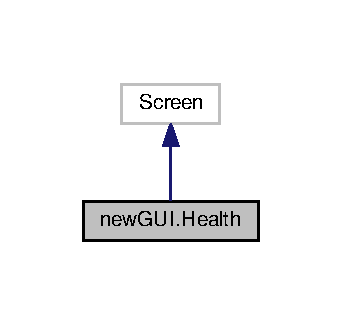
\includegraphics[width=164pt]{classnewGUI_1_1Health__inherit__graph}
\end{center}
\end{figure}


Collaboration diagram for new\+G\+U\+I.\+Health\+:
\nopagebreak
\begin{figure}[H]
\begin{center}
\leavevmode
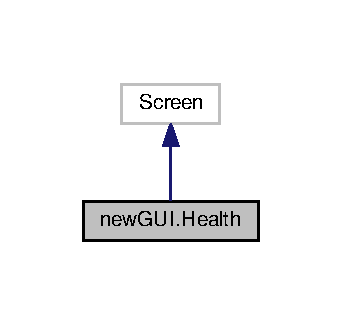
\includegraphics[width=164pt]{classnewGUI_1_1Health__coll__graph}
\end{center}
\end{figure}
\subsection*{Public Member Functions}
\begin{DoxyCompactItemize}
\item 
def \hyperlink{classnewGUI_1_1Health_a3b3a6c0877da38aff4d9c79edc49c175}{\+\_\+\+\_\+init\+\_\+\+\_\+} (self, kwargs)
\item 
def \hyperlink{classnewGUI_1_1Health_a52e48b0a6b9b6769902a3561e7bf0f29}{check\+\_\+status\+\_\+\+A\+LL} (self)
\item 
def \hyperlink{classnewGUI_1_1Health_a5d4345364392b86124613ab8bce36d21}{health\+\_\+status} (self)
\item 
def \hyperlink{classnewGUI_1_1Health_ad683313371671cdf2ec9e6bc0095b65c}{health\+\_\+popup} (self)
\item 
def \hyperlink{classnewGUI_1_1Health_a6a8e4cc7fa7dba34332f98a0dec51eba}{back\+\_\+to\+\_\+rv} (self, arg1)
\item 
def \hyperlink{classnewGUI_1_1Health_a143d001faa2f1f39f004186b94a70359}{retrieve\+Sensor} (self, ip\+\_\+addr, d)
\item 
def \hyperlink{classnewGUI_1_1Health_a319cb5153e7059ec323d578a3769c4d4}{get\+Time} (self)
\item 
def \hyperlink{classnewGUI_1_1Health_aba2a566f16ad830f2c8934dc9b1a3a5a}{retrieve\+C\+R\+\_\+and\+\_\+status} (self, hour)
\item 
def \hyperlink{classnewGUI_1_1Health_a2b3f56758a2fe65fd04d5093cb506152}{clear\+\_\+selection} (self)
\item 
def \hyperlink{classnewGUI_1_1Health_ae408bebd3ee0ad62c6dddaec1ed32df4}{status\+\_\+popup} (self)
\end{DoxyCompactItemize}
\subsection*{Static Public Attributes}
\begin{DoxyCompactItemize}
\item 
\hyperlink{classnewGUI_1_1Health_a93541d2a0ad79b7b74e07c738ede3e8e}{time} = String\+Property()
\item 
\hyperlink{classnewGUI_1_1Health_ae20ce94e54b2eed2ba31bc216016eb50}{date} = String\+Property()
\item 
\hyperlink{classnewGUI_1_1Health_a3045b67c8102d0ef4ba4511c86f8b97d}{red} = String\+Property()
\item 
\hyperlink{classnewGUI_1_1Health_a1aa34c2a1912cb021210cd5d7a2d89e7}{green} = String\+Property()
\item 
\hyperlink{classnewGUI_1_1Health_a22f818a679e9cd0affafc23025e2bae9}{blue} = String\+Property()
\item 
\hyperlink{classnewGUI_1_1Health_a783459519f248863766e8040497af001}{intensity} = String\+Property()
\item 
\hyperlink{classnewGUI_1_1Health_aa449ef4c028f2046e2c0d124e6d0f2e6}{status} = String\+Property()
\item 
\hyperlink{classnewGUI_1_1Health_abdc6fde7a65bb9c7a17de27ef65af502}{light\+\_\+name} = String\+Property()
\item 
\hyperlink{classnewGUI_1_1Health_a881213e5d35d62a75c23ce2384a125b5}{ip} = String\+Property()
\item 
\hyperlink{classnewGUI_1_1Health_a44d58ec64e7c29f44b6091fa5e84e1d3}{sa} = String\+Property()
\item 
\hyperlink{classnewGUI_1_1Health_a65c3663c4c8d9cba367a6f44e93bf924}{sr} = String\+Property()
\item 
\hyperlink{classnewGUI_1_1Health_a2fbe00b219464fe2399a667b5007754b}{sg} = String\+Property()
\item 
\hyperlink{classnewGUI_1_1Health_acf170ab735b6cfa000c2be08fe173b25}{sb} = String\+Property()
\item 
\hyperlink{classnewGUI_1_1Health_acb7c679ba6ca1fd8fb710ad0d7433a83}{A} = Numeric\+Property()
\item 
\hyperlink{classnewGUI_1_1Health_a0772a807bb2c87fca47b2cd52a0f25af}{B} = Numeric\+Property()
\item 
\hyperlink{classnewGUI_1_1Health_a966d14468b4d40cea156a0f4f4b4ae84}{R} = Numeric\+Property()
\item 
\hyperlink{classnewGUI_1_1Health_a164ba1ad352a738353b5735e96c2b8f6}{G} = Numeric\+Property()
\end{DoxyCompactItemize}


\subsection{Constructor \& Destructor Documentation}
\index{new\+G\+U\+I\+::\+Health@{new\+G\+U\+I\+::\+Health}!\+\_\+\+\_\+init\+\_\+\+\_\+@{\+\_\+\+\_\+init\+\_\+\+\_\+}}
\index{\+\_\+\+\_\+init\+\_\+\+\_\+@{\+\_\+\+\_\+init\+\_\+\+\_\+}!new\+G\+U\+I\+::\+Health@{new\+G\+U\+I\+::\+Health}}
\subsubsection[{\texorpdfstring{\+\_\+\+\_\+init\+\_\+\+\_\+(self, kwargs)}{__init__(self, kwargs)}}]{\setlength{\rightskip}{0pt plus 5cm}def new\+G\+U\+I.\+Health.\+\_\+\+\_\+init\+\_\+\+\_\+ (
\begin{DoxyParamCaption}
\item[{}]{self, }
\item[{}]{kwargs}
\end{DoxyParamCaption}
)}\hypertarget{classnewGUI_1_1Health_a3b3a6c0877da38aff4d9c79edc49c175}{}\label{classnewGUI_1_1Health_a3b3a6c0877da38aff4d9c79edc49c175}


\subsection{Member Function Documentation}
\index{new\+G\+U\+I\+::\+Health@{new\+G\+U\+I\+::\+Health}!back\+\_\+to\+\_\+rv@{back\+\_\+to\+\_\+rv}}
\index{back\+\_\+to\+\_\+rv@{back\+\_\+to\+\_\+rv}!new\+G\+U\+I\+::\+Health@{new\+G\+U\+I\+::\+Health}}
\subsubsection[{\texorpdfstring{back\+\_\+to\+\_\+rv(self, arg1)}{back_to_rv(self, arg1)}}]{\setlength{\rightskip}{0pt plus 5cm}def new\+G\+U\+I.\+Health.\+back\+\_\+to\+\_\+rv (
\begin{DoxyParamCaption}
\item[{}]{self, }
\item[{}]{arg1}
\end{DoxyParamCaption}
)}\hypertarget{classnewGUI_1_1Health_a6a8e4cc7fa7dba34332f98a0dec51eba}{}\label{classnewGUI_1_1Health_a6a8e4cc7fa7dba34332f98a0dec51eba}
\index{new\+G\+U\+I\+::\+Health@{new\+G\+U\+I\+::\+Health}!check\+\_\+status\+\_\+\+A\+LL@{check\+\_\+status\+\_\+\+A\+LL}}
\index{check\+\_\+status\+\_\+\+A\+LL@{check\+\_\+status\+\_\+\+A\+LL}!new\+G\+U\+I\+::\+Health@{new\+G\+U\+I\+::\+Health}}
\subsubsection[{\texorpdfstring{check\+\_\+status\+\_\+\+A\+L\+L(self)}{check_status_ALL(self)}}]{\setlength{\rightskip}{0pt plus 5cm}def new\+G\+U\+I.\+Health.\+check\+\_\+status\+\_\+\+A\+LL (
\begin{DoxyParamCaption}
\item[{}]{self}
\end{DoxyParamCaption}
)}\hypertarget{classnewGUI_1_1Health_a52e48b0a6b9b6769902a3561e7bf0f29}{}\label{classnewGUI_1_1Health_a52e48b0a6b9b6769902a3561e7bf0f29}
\index{new\+G\+U\+I\+::\+Health@{new\+G\+U\+I\+::\+Health}!clear\+\_\+selection@{clear\+\_\+selection}}
\index{clear\+\_\+selection@{clear\+\_\+selection}!new\+G\+U\+I\+::\+Health@{new\+G\+U\+I\+::\+Health}}
\subsubsection[{\texorpdfstring{clear\+\_\+selection(self)}{clear_selection(self)}}]{\setlength{\rightskip}{0pt plus 5cm}def new\+G\+U\+I.\+Health.\+clear\+\_\+selection (
\begin{DoxyParamCaption}
\item[{}]{self}
\end{DoxyParamCaption}
)}\hypertarget{classnewGUI_1_1Health_a2b3f56758a2fe65fd04d5093cb506152}{}\label{classnewGUI_1_1Health_a2b3f56758a2fe65fd04d5093cb506152}
\index{new\+G\+U\+I\+::\+Health@{new\+G\+U\+I\+::\+Health}!get\+Time@{get\+Time}}
\index{get\+Time@{get\+Time}!new\+G\+U\+I\+::\+Health@{new\+G\+U\+I\+::\+Health}}
\subsubsection[{\texorpdfstring{get\+Time(self)}{getTime(self)}}]{\setlength{\rightskip}{0pt plus 5cm}def new\+G\+U\+I.\+Health.\+get\+Time (
\begin{DoxyParamCaption}
\item[{}]{self}
\end{DoxyParamCaption}
)}\hypertarget{classnewGUI_1_1Health_a319cb5153e7059ec323d578a3769c4d4}{}\label{classnewGUI_1_1Health_a319cb5153e7059ec323d578a3769c4d4}
\index{new\+G\+U\+I\+::\+Health@{new\+G\+U\+I\+::\+Health}!health\+\_\+popup@{health\+\_\+popup}}
\index{health\+\_\+popup@{health\+\_\+popup}!new\+G\+U\+I\+::\+Health@{new\+G\+U\+I\+::\+Health}}
\subsubsection[{\texorpdfstring{health\+\_\+popup(self)}{health_popup(self)}}]{\setlength{\rightskip}{0pt plus 5cm}def new\+G\+U\+I.\+Health.\+health\+\_\+popup (
\begin{DoxyParamCaption}
\item[{}]{self}
\end{DoxyParamCaption}
)}\hypertarget{classnewGUI_1_1Health_ad683313371671cdf2ec9e6bc0095b65c}{}\label{classnewGUI_1_1Health_ad683313371671cdf2ec9e6bc0095b65c}
\index{new\+G\+U\+I\+::\+Health@{new\+G\+U\+I\+::\+Health}!health\+\_\+status@{health\+\_\+status}}
\index{health\+\_\+status@{health\+\_\+status}!new\+G\+U\+I\+::\+Health@{new\+G\+U\+I\+::\+Health}}
\subsubsection[{\texorpdfstring{health\+\_\+status(self)}{health_status(self)}}]{\setlength{\rightskip}{0pt plus 5cm}def new\+G\+U\+I.\+Health.\+health\+\_\+status (
\begin{DoxyParamCaption}
\item[{}]{self}
\end{DoxyParamCaption}
)}\hypertarget{classnewGUI_1_1Health_a5d4345364392b86124613ab8bce36d21}{}\label{classnewGUI_1_1Health_a5d4345364392b86124613ab8bce36d21}
\index{new\+G\+U\+I\+::\+Health@{new\+G\+U\+I\+::\+Health}!retrieve\+C\+R\+\_\+and\+\_\+status@{retrieve\+C\+R\+\_\+and\+\_\+status}}
\index{retrieve\+C\+R\+\_\+and\+\_\+status@{retrieve\+C\+R\+\_\+and\+\_\+status}!new\+G\+U\+I\+::\+Health@{new\+G\+U\+I\+::\+Health}}
\subsubsection[{\texorpdfstring{retrieve\+C\+R\+\_\+and\+\_\+status(self, hour)}{retrieveCR_and_status(self, hour)}}]{\setlength{\rightskip}{0pt plus 5cm}def new\+G\+U\+I.\+Health.\+retrieve\+C\+R\+\_\+and\+\_\+status (
\begin{DoxyParamCaption}
\item[{}]{self, }
\item[{}]{hour}
\end{DoxyParamCaption}
)}\hypertarget{classnewGUI_1_1Health_aba2a566f16ad830f2c8934dc9b1a3a5a}{}\label{classnewGUI_1_1Health_aba2a566f16ad830f2c8934dc9b1a3a5a}
\index{new\+G\+U\+I\+::\+Health@{new\+G\+U\+I\+::\+Health}!retrieve\+Sensor@{retrieve\+Sensor}}
\index{retrieve\+Sensor@{retrieve\+Sensor}!new\+G\+U\+I\+::\+Health@{new\+G\+U\+I\+::\+Health}}
\subsubsection[{\texorpdfstring{retrieve\+Sensor(self, ip\+\_\+addr, d)}{retrieveSensor(self, ip_addr, d)}}]{\setlength{\rightskip}{0pt plus 5cm}def new\+G\+U\+I.\+Health.\+retrieve\+Sensor (
\begin{DoxyParamCaption}
\item[{}]{self, }
\item[{}]{ip\+\_\+addr, }
\item[{}]{d}
\end{DoxyParamCaption}
)}\hypertarget{classnewGUI_1_1Health_a143d001faa2f1f39f004186b94a70359}{}\label{classnewGUI_1_1Health_a143d001faa2f1f39f004186b94a70359}
\index{new\+G\+U\+I\+::\+Health@{new\+G\+U\+I\+::\+Health}!status\+\_\+popup@{status\+\_\+popup}}
\index{status\+\_\+popup@{status\+\_\+popup}!new\+G\+U\+I\+::\+Health@{new\+G\+U\+I\+::\+Health}}
\subsubsection[{\texorpdfstring{status\+\_\+popup(self)}{status_popup(self)}}]{\setlength{\rightskip}{0pt plus 5cm}def new\+G\+U\+I.\+Health.\+status\+\_\+popup (
\begin{DoxyParamCaption}
\item[{}]{self}
\end{DoxyParamCaption}
)}\hypertarget{classnewGUI_1_1Health_ae408bebd3ee0ad62c6dddaec1ed32df4}{}\label{classnewGUI_1_1Health_ae408bebd3ee0ad62c6dddaec1ed32df4}


\subsection{Member Data Documentation}
\index{new\+G\+U\+I\+::\+Health@{new\+G\+U\+I\+::\+Health}!A@{A}}
\index{A@{A}!new\+G\+U\+I\+::\+Health@{new\+G\+U\+I\+::\+Health}}
\subsubsection[{\texorpdfstring{A}{A}}]{\setlength{\rightskip}{0pt plus 5cm}new\+G\+U\+I.\+Health.\+A = Numeric\+Property()\hspace{0.3cm}{\ttfamily [static]}}\hypertarget{classnewGUI_1_1Health_acb7c679ba6ca1fd8fb710ad0d7433a83}{}\label{classnewGUI_1_1Health_acb7c679ba6ca1fd8fb710ad0d7433a83}
\index{new\+G\+U\+I\+::\+Health@{new\+G\+U\+I\+::\+Health}!B@{B}}
\index{B@{B}!new\+G\+U\+I\+::\+Health@{new\+G\+U\+I\+::\+Health}}
\subsubsection[{\texorpdfstring{B}{B}}]{\setlength{\rightskip}{0pt plus 5cm}new\+G\+U\+I.\+Health.\+B = Numeric\+Property()\hspace{0.3cm}{\ttfamily [static]}}\hypertarget{classnewGUI_1_1Health_a0772a807bb2c87fca47b2cd52a0f25af}{}\label{classnewGUI_1_1Health_a0772a807bb2c87fca47b2cd52a0f25af}
\index{new\+G\+U\+I\+::\+Health@{new\+G\+U\+I\+::\+Health}!blue@{blue}}
\index{blue@{blue}!new\+G\+U\+I\+::\+Health@{new\+G\+U\+I\+::\+Health}}
\subsubsection[{\texorpdfstring{blue}{blue}}]{\setlength{\rightskip}{0pt plus 5cm}new\+G\+U\+I.\+Health.\+blue = String\+Property()\hspace{0.3cm}{\ttfamily [static]}}\hypertarget{classnewGUI_1_1Health_a22f818a679e9cd0affafc23025e2bae9}{}\label{classnewGUI_1_1Health_a22f818a679e9cd0affafc23025e2bae9}
\index{new\+G\+U\+I\+::\+Health@{new\+G\+U\+I\+::\+Health}!date@{date}}
\index{date@{date}!new\+G\+U\+I\+::\+Health@{new\+G\+U\+I\+::\+Health}}
\subsubsection[{\texorpdfstring{date}{date}}]{\setlength{\rightskip}{0pt plus 5cm}new\+G\+U\+I.\+Health.\+date = String\+Property()\hspace{0.3cm}{\ttfamily [static]}}\hypertarget{classnewGUI_1_1Health_ae20ce94e54b2eed2ba31bc216016eb50}{}\label{classnewGUI_1_1Health_ae20ce94e54b2eed2ba31bc216016eb50}
\index{new\+G\+U\+I\+::\+Health@{new\+G\+U\+I\+::\+Health}!G@{G}}
\index{G@{G}!new\+G\+U\+I\+::\+Health@{new\+G\+U\+I\+::\+Health}}
\subsubsection[{\texorpdfstring{G}{G}}]{\setlength{\rightskip}{0pt plus 5cm}new\+G\+U\+I.\+Health.\+G = Numeric\+Property()\hspace{0.3cm}{\ttfamily [static]}}\hypertarget{classnewGUI_1_1Health_a164ba1ad352a738353b5735e96c2b8f6}{}\label{classnewGUI_1_1Health_a164ba1ad352a738353b5735e96c2b8f6}
\index{new\+G\+U\+I\+::\+Health@{new\+G\+U\+I\+::\+Health}!green@{green}}
\index{green@{green}!new\+G\+U\+I\+::\+Health@{new\+G\+U\+I\+::\+Health}}
\subsubsection[{\texorpdfstring{green}{green}}]{\setlength{\rightskip}{0pt plus 5cm}new\+G\+U\+I.\+Health.\+green = String\+Property()\hspace{0.3cm}{\ttfamily [static]}}\hypertarget{classnewGUI_1_1Health_a1aa34c2a1912cb021210cd5d7a2d89e7}{}\label{classnewGUI_1_1Health_a1aa34c2a1912cb021210cd5d7a2d89e7}
\index{new\+G\+U\+I\+::\+Health@{new\+G\+U\+I\+::\+Health}!intensity@{intensity}}
\index{intensity@{intensity}!new\+G\+U\+I\+::\+Health@{new\+G\+U\+I\+::\+Health}}
\subsubsection[{\texorpdfstring{intensity}{intensity}}]{\setlength{\rightskip}{0pt plus 5cm}new\+G\+U\+I.\+Health.\+intensity = String\+Property()\hspace{0.3cm}{\ttfamily [static]}}\hypertarget{classnewGUI_1_1Health_a783459519f248863766e8040497af001}{}\label{classnewGUI_1_1Health_a783459519f248863766e8040497af001}
\index{new\+G\+U\+I\+::\+Health@{new\+G\+U\+I\+::\+Health}!ip@{ip}}
\index{ip@{ip}!new\+G\+U\+I\+::\+Health@{new\+G\+U\+I\+::\+Health}}
\subsubsection[{\texorpdfstring{ip}{ip}}]{\setlength{\rightskip}{0pt plus 5cm}new\+G\+U\+I.\+Health.\+ip = String\+Property()\hspace{0.3cm}{\ttfamily [static]}}\hypertarget{classnewGUI_1_1Health_a881213e5d35d62a75c23ce2384a125b5}{}\label{classnewGUI_1_1Health_a881213e5d35d62a75c23ce2384a125b5}
\index{new\+G\+U\+I\+::\+Health@{new\+G\+U\+I\+::\+Health}!light\+\_\+name@{light\+\_\+name}}
\index{light\+\_\+name@{light\+\_\+name}!new\+G\+U\+I\+::\+Health@{new\+G\+U\+I\+::\+Health}}
\subsubsection[{\texorpdfstring{light\+\_\+name}{light_name}}]{\setlength{\rightskip}{0pt plus 5cm}new\+G\+U\+I.\+Health.\+light\+\_\+name = String\+Property()\hspace{0.3cm}{\ttfamily [static]}}\hypertarget{classnewGUI_1_1Health_abdc6fde7a65bb9c7a17de27ef65af502}{}\label{classnewGUI_1_1Health_abdc6fde7a65bb9c7a17de27ef65af502}
\index{new\+G\+U\+I\+::\+Health@{new\+G\+U\+I\+::\+Health}!R@{R}}
\index{R@{R}!new\+G\+U\+I\+::\+Health@{new\+G\+U\+I\+::\+Health}}
\subsubsection[{\texorpdfstring{R}{R}}]{\setlength{\rightskip}{0pt plus 5cm}new\+G\+U\+I.\+Health.\+R = Numeric\+Property()\hspace{0.3cm}{\ttfamily [static]}}\hypertarget{classnewGUI_1_1Health_a966d14468b4d40cea156a0f4f4b4ae84}{}\label{classnewGUI_1_1Health_a966d14468b4d40cea156a0f4f4b4ae84}
\index{new\+G\+U\+I\+::\+Health@{new\+G\+U\+I\+::\+Health}!red@{red}}
\index{red@{red}!new\+G\+U\+I\+::\+Health@{new\+G\+U\+I\+::\+Health}}
\subsubsection[{\texorpdfstring{red}{red}}]{\setlength{\rightskip}{0pt plus 5cm}new\+G\+U\+I.\+Health.\+red = String\+Property()\hspace{0.3cm}{\ttfamily [static]}}\hypertarget{classnewGUI_1_1Health_a3045b67c8102d0ef4ba4511c86f8b97d}{}\label{classnewGUI_1_1Health_a3045b67c8102d0ef4ba4511c86f8b97d}
\index{new\+G\+U\+I\+::\+Health@{new\+G\+U\+I\+::\+Health}!sa@{sa}}
\index{sa@{sa}!new\+G\+U\+I\+::\+Health@{new\+G\+U\+I\+::\+Health}}
\subsubsection[{\texorpdfstring{sa}{sa}}]{\setlength{\rightskip}{0pt plus 5cm}new\+G\+U\+I.\+Health.\+sa = String\+Property()\hspace{0.3cm}{\ttfamily [static]}}\hypertarget{classnewGUI_1_1Health_a44d58ec64e7c29f44b6091fa5e84e1d3}{}\label{classnewGUI_1_1Health_a44d58ec64e7c29f44b6091fa5e84e1d3}
\index{new\+G\+U\+I\+::\+Health@{new\+G\+U\+I\+::\+Health}!sb@{sb}}
\index{sb@{sb}!new\+G\+U\+I\+::\+Health@{new\+G\+U\+I\+::\+Health}}
\subsubsection[{\texorpdfstring{sb}{sb}}]{\setlength{\rightskip}{0pt plus 5cm}new\+G\+U\+I.\+Health.\+sb = String\+Property()\hspace{0.3cm}{\ttfamily [static]}}\hypertarget{classnewGUI_1_1Health_acf170ab735b6cfa000c2be08fe173b25}{}\label{classnewGUI_1_1Health_acf170ab735b6cfa000c2be08fe173b25}
\index{new\+G\+U\+I\+::\+Health@{new\+G\+U\+I\+::\+Health}!sg@{sg}}
\index{sg@{sg}!new\+G\+U\+I\+::\+Health@{new\+G\+U\+I\+::\+Health}}
\subsubsection[{\texorpdfstring{sg}{sg}}]{\setlength{\rightskip}{0pt plus 5cm}new\+G\+U\+I.\+Health.\+sg = String\+Property()\hspace{0.3cm}{\ttfamily [static]}}\hypertarget{classnewGUI_1_1Health_a2fbe00b219464fe2399a667b5007754b}{}\label{classnewGUI_1_1Health_a2fbe00b219464fe2399a667b5007754b}
\index{new\+G\+U\+I\+::\+Health@{new\+G\+U\+I\+::\+Health}!sr@{sr}}
\index{sr@{sr}!new\+G\+U\+I\+::\+Health@{new\+G\+U\+I\+::\+Health}}
\subsubsection[{\texorpdfstring{sr}{sr}}]{\setlength{\rightskip}{0pt plus 5cm}new\+G\+U\+I.\+Health.\+sr = String\+Property()\hspace{0.3cm}{\ttfamily [static]}}\hypertarget{classnewGUI_1_1Health_a65c3663c4c8d9cba367a6f44e93bf924}{}\label{classnewGUI_1_1Health_a65c3663c4c8d9cba367a6f44e93bf924}
\index{new\+G\+U\+I\+::\+Health@{new\+G\+U\+I\+::\+Health}!status@{status}}
\index{status@{status}!new\+G\+U\+I\+::\+Health@{new\+G\+U\+I\+::\+Health}}
\subsubsection[{\texorpdfstring{status}{status}}]{\setlength{\rightskip}{0pt plus 5cm}new\+G\+U\+I.\+Health.\+status = String\+Property()\hspace{0.3cm}{\ttfamily [static]}}\hypertarget{classnewGUI_1_1Health_aa449ef4c028f2046e2c0d124e6d0f2e6}{}\label{classnewGUI_1_1Health_aa449ef4c028f2046e2c0d124e6d0f2e6}
\index{new\+G\+U\+I\+::\+Health@{new\+G\+U\+I\+::\+Health}!time@{time}}
\index{time@{time}!new\+G\+U\+I\+::\+Health@{new\+G\+U\+I\+::\+Health}}
\subsubsection[{\texorpdfstring{time}{time}}]{\setlength{\rightskip}{0pt plus 5cm}new\+G\+U\+I.\+Health.\+time = String\+Property()\hspace{0.3cm}{\ttfamily [static]}}\hypertarget{classnewGUI_1_1Health_a93541d2a0ad79b7b74e07c738ede3e8e}{}\label{classnewGUI_1_1Health_a93541d2a0ad79b7b74e07c738ede3e8e}


The documentation for this class was generated from the following file\+:\begin{DoxyCompactItemize}
\item 
/home/jac0656/\+Desktop/\+J-\/\+O-\/\+R-\/\+G-\/\+E/\+U\+N\+T-\/\+N\+A\+S\+A/\+G\+U\+I/\hyperlink{newGUI_8py}{new\+G\+U\+I.\+py}\end{DoxyCompactItemize}

\hypertarget{classGUI8-5pm_1_1Health}{}\section{G\+U\+I8-\/5pm.Health Class Reference}
\label{classGUI8-5pm_1_1Health}\index{G\+U\+I8-\/5pm.\+Health@{G\+U\+I8-\/5pm.\+Health}}


Inheritance diagram for G\+U\+I8-\/5pm.Health\+:
\nopagebreak
\begin{figure}[H]
\begin{center}
\leavevmode
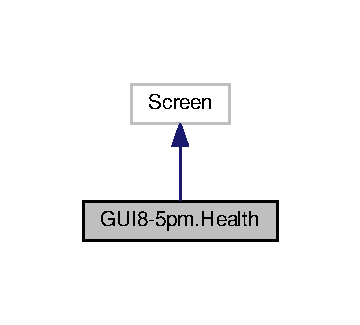
\includegraphics[width=173pt]{classGUI8-5pm_1_1Health__inherit__graph}
\end{center}
\end{figure}


Collaboration diagram for G\+U\+I8-\/5pm.Health\+:
\nopagebreak
\begin{figure}[H]
\begin{center}
\leavevmode
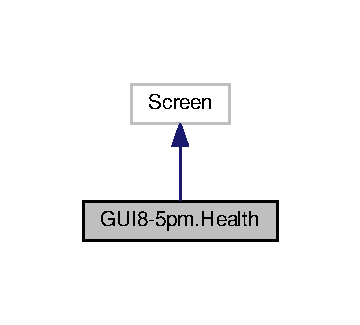
\includegraphics[width=173pt]{classGUI8-5pm_1_1Health__coll__graph}
\end{center}
\end{figure}
\subsection*{Public Member Functions}
\begin{DoxyCompactItemize}
\item 
def \hyperlink{classGUI8-5pm_1_1Health_aca55a65ec04388914fb78a8ca73dba48}{\+\_\+\+\_\+init\+\_\+\+\_\+} (self, kwargs)
\item 
def \hyperlink{classGUI8-5pm_1_1Health_ab782b2a71481d6a130c795eab53fe75e}{check\+\_\+status\+\_\+\+A\+LL} (self)
\item 
def \hyperlink{classGUI8-5pm_1_1Health_ae401ab40e875971d01975d3baa460a62}{health\+\_\+status} (self)
\item 
def \hyperlink{classGUI8-5pm_1_1Health_afb22369f48e93c061f9a419475dc73ac}{health\+\_\+popup} (self)
\item 
def \hyperlink{classGUI8-5pm_1_1Health_ac495b4ed1bfabddfeda427058b677483}{back\+\_\+to\+\_\+rv} (self, arg1)
\item 
def \hyperlink{classGUI8-5pm_1_1Health_a987bf153d5171410881f3d465d8a1a67}{retrieve\+Sensor} (self, ip\+\_\+addr, d)
\item 
def \hyperlink{classGUI8-5pm_1_1Health_ac99930874e77f0237f93ace55f9521a2}{get\+Time} (self)
\item 
def \hyperlink{classGUI8-5pm_1_1Health_afda2c200de90c8a04ec65d1cf6e3fced}{retrieve\+C\+R\+\_\+and\+\_\+status} (self, hour)
\item 
def \hyperlink{classGUI8-5pm_1_1Health_aba4ec07d15f91f98a3d7d7b2fe95a925}{clear\+\_\+selection} (self)
\item 
def \hyperlink{classGUI8-5pm_1_1Health_a763c9be087d837662bdf26cea606fce8}{status\+\_\+popup} (self)
\end{DoxyCompactItemize}
\subsection*{Static Public Attributes}
\begin{DoxyCompactItemize}
\item 
\hyperlink{classGUI8-5pm_1_1Health_aab9c45abe8afaa3d8193cde79882997b}{time} = String\+Property()
\item 
\hyperlink{classGUI8-5pm_1_1Health_acc485e524fc05b9ca82b6569521e5a63}{date} = String\+Property()
\item 
\hyperlink{classGUI8-5pm_1_1Health_a778600d7839c92633e9e832547af5fed}{red} = String\+Property()
\item 
\hyperlink{classGUI8-5pm_1_1Health_aed2a9d5c98eb7ac9634b5bd0adf5ee2e}{green} = String\+Property()
\item 
\hyperlink{classGUI8-5pm_1_1Health_a8ac8026c56d255faeab8d4afe21ec5bb}{blue} = String\+Property()
\item 
\hyperlink{classGUI8-5pm_1_1Health_a45a1c2ab6a17dc1727232cfaa74908ed}{intensity} = String\+Property()
\item 
\hyperlink{classGUI8-5pm_1_1Health_a84aa8f95f5e3d9e5cfcccc6a27e6d4e2}{status} = String\+Property()
\item 
\hyperlink{classGUI8-5pm_1_1Health_aef04a9b216ae42f919c44b7e579f5e19}{light\+\_\+name} = String\+Property()
\item 
\hyperlink{classGUI8-5pm_1_1Health_af7e3ae7115d08325af51c6df6cd00b9f}{ip} = String\+Property()
\item 
\hyperlink{classGUI8-5pm_1_1Health_a85672c208d494e85bcf03c9f4f7236d9}{sa} = String\+Property()
\item 
\hyperlink{classGUI8-5pm_1_1Health_a9078619f648e81b2741764d28e22e848}{sr} = String\+Property()
\item 
\hyperlink{classGUI8-5pm_1_1Health_af1b327e9e98e85b627830fa16b6e3a78}{sg} = String\+Property()
\item 
\hyperlink{classGUI8-5pm_1_1Health_a079adb78711dc4524435e0a88f05ccf1}{sb} = String\+Property()
\item 
\hyperlink{classGUI8-5pm_1_1Health_a7790740d8f757221bc53234c356cc1f1}{A} = Numeric\+Property()
\item 
\hyperlink{classGUI8-5pm_1_1Health_a6feaf93dec13e83ab0a8b01f295bae12}{B} = Numeric\+Property()
\item 
\hyperlink{classGUI8-5pm_1_1Health_af4bfb33acb56f8b0b477c836dcc0ddd8}{R} = Numeric\+Property()
\item 
\hyperlink{classGUI8-5pm_1_1Health_ab5930d4acd1d820a42439f7e755ceef6}{G} = Numeric\+Property()
\end{DoxyCompactItemize}


\subsection{Constructor \& Destructor Documentation}
\index{G\+U\+I8-\/5pm\+::\+Health@{G\+U\+I8-\/5pm\+::\+Health}!\+\_\+\+\_\+init\+\_\+\+\_\+@{\+\_\+\+\_\+init\+\_\+\+\_\+}}
\index{\+\_\+\+\_\+init\+\_\+\+\_\+@{\+\_\+\+\_\+init\+\_\+\+\_\+}!G\+U\+I8-\/5pm\+::\+Health@{G\+U\+I8-\/5pm\+::\+Health}}
\subsubsection[{\texorpdfstring{\+\_\+\+\_\+init\+\_\+\+\_\+(self, kwargs)}{__init__(self, kwargs)}}]{\setlength{\rightskip}{0pt plus 5cm}def G\+U\+I8-\/5pm.\+Health.\+\_\+\+\_\+init\+\_\+\+\_\+ (
\begin{DoxyParamCaption}
\item[{}]{self, }
\item[{}]{kwargs}
\end{DoxyParamCaption}
)}\hypertarget{classGUI8-5pm_1_1Health_aca55a65ec04388914fb78a8ca73dba48}{}\label{classGUI8-5pm_1_1Health_aca55a65ec04388914fb78a8ca73dba48}


\subsection{Member Function Documentation}
\index{G\+U\+I8-\/5pm\+::\+Health@{G\+U\+I8-\/5pm\+::\+Health}!back\+\_\+to\+\_\+rv@{back\+\_\+to\+\_\+rv}}
\index{back\+\_\+to\+\_\+rv@{back\+\_\+to\+\_\+rv}!G\+U\+I8-\/5pm\+::\+Health@{G\+U\+I8-\/5pm\+::\+Health}}
\subsubsection[{\texorpdfstring{back\+\_\+to\+\_\+rv(self, arg1)}{back_to_rv(self, arg1)}}]{\setlength{\rightskip}{0pt plus 5cm}def G\+U\+I8-\/5pm.\+Health.\+back\+\_\+to\+\_\+rv (
\begin{DoxyParamCaption}
\item[{}]{self, }
\item[{}]{arg1}
\end{DoxyParamCaption}
)}\hypertarget{classGUI8-5pm_1_1Health_ac495b4ed1bfabddfeda427058b677483}{}\label{classGUI8-5pm_1_1Health_ac495b4ed1bfabddfeda427058b677483}
\index{G\+U\+I8-\/5pm\+::\+Health@{G\+U\+I8-\/5pm\+::\+Health}!check\+\_\+status\+\_\+\+A\+LL@{check\+\_\+status\+\_\+\+A\+LL}}
\index{check\+\_\+status\+\_\+\+A\+LL@{check\+\_\+status\+\_\+\+A\+LL}!G\+U\+I8-\/5pm\+::\+Health@{G\+U\+I8-\/5pm\+::\+Health}}
\subsubsection[{\texorpdfstring{check\+\_\+status\+\_\+\+A\+L\+L(self)}{check_status_ALL(self)}}]{\setlength{\rightskip}{0pt plus 5cm}def G\+U\+I8-\/5pm.\+Health.\+check\+\_\+status\+\_\+\+A\+LL (
\begin{DoxyParamCaption}
\item[{}]{self}
\end{DoxyParamCaption}
)}\hypertarget{classGUI8-5pm_1_1Health_ab782b2a71481d6a130c795eab53fe75e}{}\label{classGUI8-5pm_1_1Health_ab782b2a71481d6a130c795eab53fe75e}
\index{G\+U\+I8-\/5pm\+::\+Health@{G\+U\+I8-\/5pm\+::\+Health}!clear\+\_\+selection@{clear\+\_\+selection}}
\index{clear\+\_\+selection@{clear\+\_\+selection}!G\+U\+I8-\/5pm\+::\+Health@{G\+U\+I8-\/5pm\+::\+Health}}
\subsubsection[{\texorpdfstring{clear\+\_\+selection(self)}{clear_selection(self)}}]{\setlength{\rightskip}{0pt plus 5cm}def G\+U\+I8-\/5pm.\+Health.\+clear\+\_\+selection (
\begin{DoxyParamCaption}
\item[{}]{self}
\end{DoxyParamCaption}
)}\hypertarget{classGUI8-5pm_1_1Health_aba4ec07d15f91f98a3d7d7b2fe95a925}{}\label{classGUI8-5pm_1_1Health_aba4ec07d15f91f98a3d7d7b2fe95a925}
\index{G\+U\+I8-\/5pm\+::\+Health@{G\+U\+I8-\/5pm\+::\+Health}!get\+Time@{get\+Time}}
\index{get\+Time@{get\+Time}!G\+U\+I8-\/5pm\+::\+Health@{G\+U\+I8-\/5pm\+::\+Health}}
\subsubsection[{\texorpdfstring{get\+Time(self)}{getTime(self)}}]{\setlength{\rightskip}{0pt plus 5cm}def G\+U\+I8-\/5pm.\+Health.\+get\+Time (
\begin{DoxyParamCaption}
\item[{}]{self}
\end{DoxyParamCaption}
)}\hypertarget{classGUI8-5pm_1_1Health_ac99930874e77f0237f93ace55f9521a2}{}\label{classGUI8-5pm_1_1Health_ac99930874e77f0237f93ace55f9521a2}
\index{G\+U\+I8-\/5pm\+::\+Health@{G\+U\+I8-\/5pm\+::\+Health}!health\+\_\+popup@{health\+\_\+popup}}
\index{health\+\_\+popup@{health\+\_\+popup}!G\+U\+I8-\/5pm\+::\+Health@{G\+U\+I8-\/5pm\+::\+Health}}
\subsubsection[{\texorpdfstring{health\+\_\+popup(self)}{health_popup(self)}}]{\setlength{\rightskip}{0pt plus 5cm}def G\+U\+I8-\/5pm.\+Health.\+health\+\_\+popup (
\begin{DoxyParamCaption}
\item[{}]{self}
\end{DoxyParamCaption}
)}\hypertarget{classGUI8-5pm_1_1Health_afb22369f48e93c061f9a419475dc73ac}{}\label{classGUI8-5pm_1_1Health_afb22369f48e93c061f9a419475dc73ac}
\index{G\+U\+I8-\/5pm\+::\+Health@{G\+U\+I8-\/5pm\+::\+Health}!health\+\_\+status@{health\+\_\+status}}
\index{health\+\_\+status@{health\+\_\+status}!G\+U\+I8-\/5pm\+::\+Health@{G\+U\+I8-\/5pm\+::\+Health}}
\subsubsection[{\texorpdfstring{health\+\_\+status(self)}{health_status(self)}}]{\setlength{\rightskip}{0pt plus 5cm}def G\+U\+I8-\/5pm.\+Health.\+health\+\_\+status (
\begin{DoxyParamCaption}
\item[{}]{self}
\end{DoxyParamCaption}
)}\hypertarget{classGUI8-5pm_1_1Health_ae401ab40e875971d01975d3baa460a62}{}\label{classGUI8-5pm_1_1Health_ae401ab40e875971d01975d3baa460a62}
\index{G\+U\+I8-\/5pm\+::\+Health@{G\+U\+I8-\/5pm\+::\+Health}!retrieve\+C\+R\+\_\+and\+\_\+status@{retrieve\+C\+R\+\_\+and\+\_\+status}}
\index{retrieve\+C\+R\+\_\+and\+\_\+status@{retrieve\+C\+R\+\_\+and\+\_\+status}!G\+U\+I8-\/5pm\+::\+Health@{G\+U\+I8-\/5pm\+::\+Health}}
\subsubsection[{\texorpdfstring{retrieve\+C\+R\+\_\+and\+\_\+status(self, hour)}{retrieveCR_and_status(self, hour)}}]{\setlength{\rightskip}{0pt plus 5cm}def G\+U\+I8-\/5pm.\+Health.\+retrieve\+C\+R\+\_\+and\+\_\+status (
\begin{DoxyParamCaption}
\item[{}]{self, }
\item[{}]{hour}
\end{DoxyParamCaption}
)}\hypertarget{classGUI8-5pm_1_1Health_afda2c200de90c8a04ec65d1cf6e3fced}{}\label{classGUI8-5pm_1_1Health_afda2c200de90c8a04ec65d1cf6e3fced}
\index{G\+U\+I8-\/5pm\+::\+Health@{G\+U\+I8-\/5pm\+::\+Health}!retrieve\+Sensor@{retrieve\+Sensor}}
\index{retrieve\+Sensor@{retrieve\+Sensor}!G\+U\+I8-\/5pm\+::\+Health@{G\+U\+I8-\/5pm\+::\+Health}}
\subsubsection[{\texorpdfstring{retrieve\+Sensor(self, ip\+\_\+addr, d)}{retrieveSensor(self, ip_addr, d)}}]{\setlength{\rightskip}{0pt plus 5cm}def G\+U\+I8-\/5pm.\+Health.\+retrieve\+Sensor (
\begin{DoxyParamCaption}
\item[{}]{self, }
\item[{}]{ip\+\_\+addr, }
\item[{}]{d}
\end{DoxyParamCaption}
)}\hypertarget{classGUI8-5pm_1_1Health_a987bf153d5171410881f3d465d8a1a67}{}\label{classGUI8-5pm_1_1Health_a987bf153d5171410881f3d465d8a1a67}
\index{G\+U\+I8-\/5pm\+::\+Health@{G\+U\+I8-\/5pm\+::\+Health}!status\+\_\+popup@{status\+\_\+popup}}
\index{status\+\_\+popup@{status\+\_\+popup}!G\+U\+I8-\/5pm\+::\+Health@{G\+U\+I8-\/5pm\+::\+Health}}
\subsubsection[{\texorpdfstring{status\+\_\+popup(self)}{status_popup(self)}}]{\setlength{\rightskip}{0pt plus 5cm}def G\+U\+I8-\/5pm.\+Health.\+status\+\_\+popup (
\begin{DoxyParamCaption}
\item[{}]{self}
\end{DoxyParamCaption}
)}\hypertarget{classGUI8-5pm_1_1Health_a763c9be087d837662bdf26cea606fce8}{}\label{classGUI8-5pm_1_1Health_a763c9be087d837662bdf26cea606fce8}


\subsection{Member Data Documentation}
\index{G\+U\+I8-\/5pm\+::\+Health@{G\+U\+I8-\/5pm\+::\+Health}!A@{A}}
\index{A@{A}!G\+U\+I8-\/5pm\+::\+Health@{G\+U\+I8-\/5pm\+::\+Health}}
\subsubsection[{\texorpdfstring{A}{A}}]{\setlength{\rightskip}{0pt plus 5cm}G\+U\+I8-\/5pm.\+Health.\+A = Numeric\+Property()\hspace{0.3cm}{\ttfamily [static]}}\hypertarget{classGUI8-5pm_1_1Health_a7790740d8f757221bc53234c356cc1f1}{}\label{classGUI8-5pm_1_1Health_a7790740d8f757221bc53234c356cc1f1}
\index{G\+U\+I8-\/5pm\+::\+Health@{G\+U\+I8-\/5pm\+::\+Health}!B@{B}}
\index{B@{B}!G\+U\+I8-\/5pm\+::\+Health@{G\+U\+I8-\/5pm\+::\+Health}}
\subsubsection[{\texorpdfstring{B}{B}}]{\setlength{\rightskip}{0pt plus 5cm}G\+U\+I8-\/5pm.\+Health.\+B = Numeric\+Property()\hspace{0.3cm}{\ttfamily [static]}}\hypertarget{classGUI8-5pm_1_1Health_a6feaf93dec13e83ab0a8b01f295bae12}{}\label{classGUI8-5pm_1_1Health_a6feaf93dec13e83ab0a8b01f295bae12}
\index{G\+U\+I8-\/5pm\+::\+Health@{G\+U\+I8-\/5pm\+::\+Health}!blue@{blue}}
\index{blue@{blue}!G\+U\+I8-\/5pm\+::\+Health@{G\+U\+I8-\/5pm\+::\+Health}}
\subsubsection[{\texorpdfstring{blue}{blue}}]{\setlength{\rightskip}{0pt plus 5cm}G\+U\+I8-\/5pm.\+Health.\+blue = String\+Property()\hspace{0.3cm}{\ttfamily [static]}}\hypertarget{classGUI8-5pm_1_1Health_a8ac8026c56d255faeab8d4afe21ec5bb}{}\label{classGUI8-5pm_1_1Health_a8ac8026c56d255faeab8d4afe21ec5bb}
\index{G\+U\+I8-\/5pm\+::\+Health@{G\+U\+I8-\/5pm\+::\+Health}!date@{date}}
\index{date@{date}!G\+U\+I8-\/5pm\+::\+Health@{G\+U\+I8-\/5pm\+::\+Health}}
\subsubsection[{\texorpdfstring{date}{date}}]{\setlength{\rightskip}{0pt plus 5cm}G\+U\+I8-\/5pm.\+Health.\+date = String\+Property()\hspace{0.3cm}{\ttfamily [static]}}\hypertarget{classGUI8-5pm_1_1Health_acc485e524fc05b9ca82b6569521e5a63}{}\label{classGUI8-5pm_1_1Health_acc485e524fc05b9ca82b6569521e5a63}
\index{G\+U\+I8-\/5pm\+::\+Health@{G\+U\+I8-\/5pm\+::\+Health}!G@{G}}
\index{G@{G}!G\+U\+I8-\/5pm\+::\+Health@{G\+U\+I8-\/5pm\+::\+Health}}
\subsubsection[{\texorpdfstring{G}{G}}]{\setlength{\rightskip}{0pt plus 5cm}G\+U\+I8-\/5pm.\+Health.\+G = Numeric\+Property()\hspace{0.3cm}{\ttfamily [static]}}\hypertarget{classGUI8-5pm_1_1Health_ab5930d4acd1d820a42439f7e755ceef6}{}\label{classGUI8-5pm_1_1Health_ab5930d4acd1d820a42439f7e755ceef6}
\index{G\+U\+I8-\/5pm\+::\+Health@{G\+U\+I8-\/5pm\+::\+Health}!green@{green}}
\index{green@{green}!G\+U\+I8-\/5pm\+::\+Health@{G\+U\+I8-\/5pm\+::\+Health}}
\subsubsection[{\texorpdfstring{green}{green}}]{\setlength{\rightskip}{0pt plus 5cm}G\+U\+I8-\/5pm.\+Health.\+green = String\+Property()\hspace{0.3cm}{\ttfamily [static]}}\hypertarget{classGUI8-5pm_1_1Health_aed2a9d5c98eb7ac9634b5bd0adf5ee2e}{}\label{classGUI8-5pm_1_1Health_aed2a9d5c98eb7ac9634b5bd0adf5ee2e}
\index{G\+U\+I8-\/5pm\+::\+Health@{G\+U\+I8-\/5pm\+::\+Health}!intensity@{intensity}}
\index{intensity@{intensity}!G\+U\+I8-\/5pm\+::\+Health@{G\+U\+I8-\/5pm\+::\+Health}}
\subsubsection[{\texorpdfstring{intensity}{intensity}}]{\setlength{\rightskip}{0pt plus 5cm}G\+U\+I8-\/5pm.\+Health.\+intensity = String\+Property()\hspace{0.3cm}{\ttfamily [static]}}\hypertarget{classGUI8-5pm_1_1Health_a45a1c2ab6a17dc1727232cfaa74908ed}{}\label{classGUI8-5pm_1_1Health_a45a1c2ab6a17dc1727232cfaa74908ed}
\index{G\+U\+I8-\/5pm\+::\+Health@{G\+U\+I8-\/5pm\+::\+Health}!ip@{ip}}
\index{ip@{ip}!G\+U\+I8-\/5pm\+::\+Health@{G\+U\+I8-\/5pm\+::\+Health}}
\subsubsection[{\texorpdfstring{ip}{ip}}]{\setlength{\rightskip}{0pt plus 5cm}G\+U\+I8-\/5pm.\+Health.\+ip = String\+Property()\hspace{0.3cm}{\ttfamily [static]}}\hypertarget{classGUI8-5pm_1_1Health_af7e3ae7115d08325af51c6df6cd00b9f}{}\label{classGUI8-5pm_1_1Health_af7e3ae7115d08325af51c6df6cd00b9f}
\index{G\+U\+I8-\/5pm\+::\+Health@{G\+U\+I8-\/5pm\+::\+Health}!light\+\_\+name@{light\+\_\+name}}
\index{light\+\_\+name@{light\+\_\+name}!G\+U\+I8-\/5pm\+::\+Health@{G\+U\+I8-\/5pm\+::\+Health}}
\subsubsection[{\texorpdfstring{light\+\_\+name}{light_name}}]{\setlength{\rightskip}{0pt plus 5cm}G\+U\+I8-\/5pm.\+Health.\+light\+\_\+name = String\+Property()\hspace{0.3cm}{\ttfamily [static]}}\hypertarget{classGUI8-5pm_1_1Health_aef04a9b216ae42f919c44b7e579f5e19}{}\label{classGUI8-5pm_1_1Health_aef04a9b216ae42f919c44b7e579f5e19}
\index{G\+U\+I8-\/5pm\+::\+Health@{G\+U\+I8-\/5pm\+::\+Health}!R@{R}}
\index{R@{R}!G\+U\+I8-\/5pm\+::\+Health@{G\+U\+I8-\/5pm\+::\+Health}}
\subsubsection[{\texorpdfstring{R}{R}}]{\setlength{\rightskip}{0pt plus 5cm}G\+U\+I8-\/5pm.\+Health.\+R = Numeric\+Property()\hspace{0.3cm}{\ttfamily [static]}}\hypertarget{classGUI8-5pm_1_1Health_af4bfb33acb56f8b0b477c836dcc0ddd8}{}\label{classGUI8-5pm_1_1Health_af4bfb33acb56f8b0b477c836dcc0ddd8}
\index{G\+U\+I8-\/5pm\+::\+Health@{G\+U\+I8-\/5pm\+::\+Health}!red@{red}}
\index{red@{red}!G\+U\+I8-\/5pm\+::\+Health@{G\+U\+I8-\/5pm\+::\+Health}}
\subsubsection[{\texorpdfstring{red}{red}}]{\setlength{\rightskip}{0pt plus 5cm}G\+U\+I8-\/5pm.\+Health.\+red = String\+Property()\hspace{0.3cm}{\ttfamily [static]}}\hypertarget{classGUI8-5pm_1_1Health_a778600d7839c92633e9e832547af5fed}{}\label{classGUI8-5pm_1_1Health_a778600d7839c92633e9e832547af5fed}
\index{G\+U\+I8-\/5pm\+::\+Health@{G\+U\+I8-\/5pm\+::\+Health}!sa@{sa}}
\index{sa@{sa}!G\+U\+I8-\/5pm\+::\+Health@{G\+U\+I8-\/5pm\+::\+Health}}
\subsubsection[{\texorpdfstring{sa}{sa}}]{\setlength{\rightskip}{0pt plus 5cm}G\+U\+I8-\/5pm.\+Health.\+sa = String\+Property()\hspace{0.3cm}{\ttfamily [static]}}\hypertarget{classGUI8-5pm_1_1Health_a85672c208d494e85bcf03c9f4f7236d9}{}\label{classGUI8-5pm_1_1Health_a85672c208d494e85bcf03c9f4f7236d9}
\index{G\+U\+I8-\/5pm\+::\+Health@{G\+U\+I8-\/5pm\+::\+Health}!sb@{sb}}
\index{sb@{sb}!G\+U\+I8-\/5pm\+::\+Health@{G\+U\+I8-\/5pm\+::\+Health}}
\subsubsection[{\texorpdfstring{sb}{sb}}]{\setlength{\rightskip}{0pt plus 5cm}G\+U\+I8-\/5pm.\+Health.\+sb = String\+Property()\hspace{0.3cm}{\ttfamily [static]}}\hypertarget{classGUI8-5pm_1_1Health_a079adb78711dc4524435e0a88f05ccf1}{}\label{classGUI8-5pm_1_1Health_a079adb78711dc4524435e0a88f05ccf1}
\index{G\+U\+I8-\/5pm\+::\+Health@{G\+U\+I8-\/5pm\+::\+Health}!sg@{sg}}
\index{sg@{sg}!G\+U\+I8-\/5pm\+::\+Health@{G\+U\+I8-\/5pm\+::\+Health}}
\subsubsection[{\texorpdfstring{sg}{sg}}]{\setlength{\rightskip}{0pt plus 5cm}G\+U\+I8-\/5pm.\+Health.\+sg = String\+Property()\hspace{0.3cm}{\ttfamily [static]}}\hypertarget{classGUI8-5pm_1_1Health_af1b327e9e98e85b627830fa16b6e3a78}{}\label{classGUI8-5pm_1_1Health_af1b327e9e98e85b627830fa16b6e3a78}
\index{G\+U\+I8-\/5pm\+::\+Health@{G\+U\+I8-\/5pm\+::\+Health}!sr@{sr}}
\index{sr@{sr}!G\+U\+I8-\/5pm\+::\+Health@{G\+U\+I8-\/5pm\+::\+Health}}
\subsubsection[{\texorpdfstring{sr}{sr}}]{\setlength{\rightskip}{0pt plus 5cm}G\+U\+I8-\/5pm.\+Health.\+sr = String\+Property()\hspace{0.3cm}{\ttfamily [static]}}\hypertarget{classGUI8-5pm_1_1Health_a9078619f648e81b2741764d28e22e848}{}\label{classGUI8-5pm_1_1Health_a9078619f648e81b2741764d28e22e848}
\index{G\+U\+I8-\/5pm\+::\+Health@{G\+U\+I8-\/5pm\+::\+Health}!status@{status}}
\index{status@{status}!G\+U\+I8-\/5pm\+::\+Health@{G\+U\+I8-\/5pm\+::\+Health}}
\subsubsection[{\texorpdfstring{status}{status}}]{\setlength{\rightskip}{0pt plus 5cm}G\+U\+I8-\/5pm.\+Health.\+status = String\+Property()\hspace{0.3cm}{\ttfamily [static]}}\hypertarget{classGUI8-5pm_1_1Health_a84aa8f95f5e3d9e5cfcccc6a27e6d4e2}{}\label{classGUI8-5pm_1_1Health_a84aa8f95f5e3d9e5cfcccc6a27e6d4e2}
\index{G\+U\+I8-\/5pm\+::\+Health@{G\+U\+I8-\/5pm\+::\+Health}!time@{time}}
\index{time@{time}!G\+U\+I8-\/5pm\+::\+Health@{G\+U\+I8-\/5pm\+::\+Health}}
\subsubsection[{\texorpdfstring{time}{time}}]{\setlength{\rightskip}{0pt plus 5cm}G\+U\+I8-\/5pm.\+Health.\+time = String\+Property()\hspace{0.3cm}{\ttfamily [static]}}\hypertarget{classGUI8-5pm_1_1Health_aab9c45abe8afaa3d8193cde79882997b}{}\label{classGUI8-5pm_1_1Health_aab9c45abe8afaa3d8193cde79882997b}


The documentation for this class was generated from the following file\+:\begin{DoxyCompactItemize}
\item 
/home/jac0656/\+Desktop/\+J-\/\+O-\/\+R-\/\+G-\/\+E/\+U\+N\+T-\/\+N\+A\+S\+A/\hyperlink{GUI8-5pm_8py}{G\+U\+I8-\/5pm.\+py}\end{DoxyCompactItemize}

\hypertarget{classnewGUI_1_1HomePage}{}\section{new\+G\+U\+I.\+Home\+Page Class Reference}
\label{classnewGUI_1_1HomePage}\index{new\+G\+U\+I.\+Home\+Page@{new\+G\+U\+I.\+Home\+Page}}


Inheritance diagram for new\+G\+U\+I.\+Home\+Page\+:
\nopagebreak
\begin{figure}[H]
\begin{center}
\leavevmode
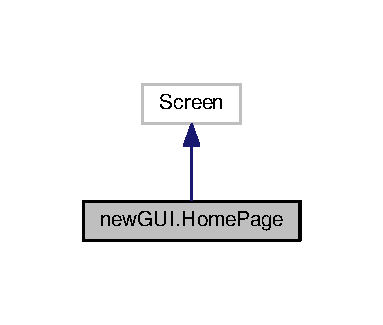
\includegraphics[width=184pt]{classnewGUI_1_1HomePage__inherit__graph}
\end{center}
\end{figure}


Collaboration diagram for new\+G\+U\+I.\+Home\+Page\+:
\nopagebreak
\begin{figure}[H]
\begin{center}
\leavevmode
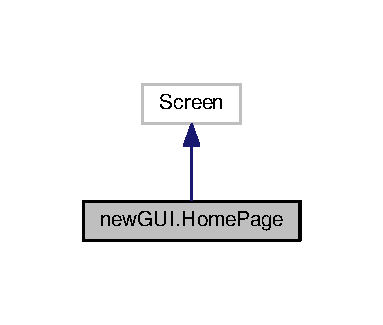
\includegraphics[width=184pt]{classnewGUI_1_1HomePage__coll__graph}
\end{center}
\end{figure}


The documentation for this class was generated from the following file\+:\begin{DoxyCompactItemize}
\item 
/home/jac0656/\+Desktop/\+J-\/\+O-\/\+R-\/\+G-\/\+E/\+U\+N\+T-\/\+N\+A\+S\+A/\+G\+U\+I/\hyperlink{newGUI_8py}{new\+G\+U\+I.\+py}\end{DoxyCompactItemize}

\hypertarget{classGUI8_1_1HomePage}{}\section{G\+U\+I8.\+Home\+Page Class Reference}
\label{classGUI8_1_1HomePage}\index{G\+U\+I8.\+Home\+Page@{G\+U\+I8.\+Home\+Page}}


Inheritance diagram for G\+U\+I8.\+Home\+Page\+:
\nopagebreak
\begin{figure}[H]
\begin{center}
\leavevmode
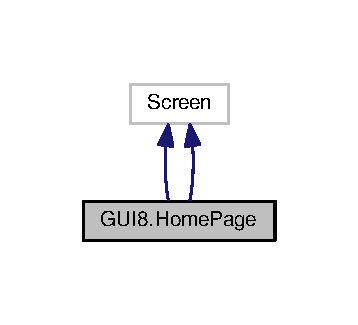
\includegraphics[width=172pt]{classGUI8_1_1HomePage__inherit__graph}
\end{center}
\end{figure}


Collaboration diagram for G\+U\+I8.\+Home\+Page\+:
\nopagebreak
\begin{figure}[H]
\begin{center}
\leavevmode
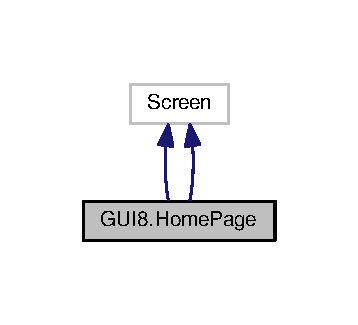
\includegraphics[width=172pt]{classGUI8_1_1HomePage__coll__graph}
\end{center}
\end{figure}


The documentation for this class was generated from the following file\+:\begin{DoxyCompactItemize}
\item 
/home/jac0656/\+Desktop/\+J-\/\+O-\/\+R-\/\+G-\/\+E/\+U\+N\+T-\/\+N\+A\+S\+A/\+G\+U\+I/\hyperlink{GUI_2GUI8_8py}{G\+U\+I8.\+py}\end{DoxyCompactItemize}

\hypertarget{classTestApp1_1_1HomePage}{}\section{Test\+App1.\+Home\+Page Class Reference}
\label{classTestApp1_1_1HomePage}\index{Test\+App1.\+Home\+Page@{Test\+App1.\+Home\+Page}}


Inheritance diagram for Test\+App1.\+Home\+Page\+:
\nopagebreak
\begin{figure}[H]
\begin{center}
\leavevmode
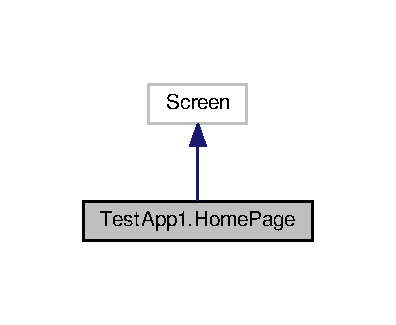
\includegraphics[width=190pt]{classTestApp1_1_1HomePage__inherit__graph}
\end{center}
\end{figure}


Collaboration diagram for Test\+App1.\+Home\+Page\+:
\nopagebreak
\begin{figure}[H]
\begin{center}
\leavevmode
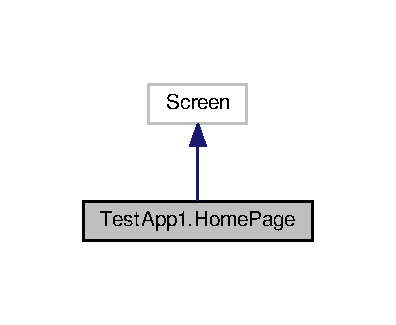
\includegraphics[width=190pt]{classTestApp1_1_1HomePage__coll__graph}
\end{center}
\end{figure}


The documentation for this class was generated from the following file\+:\begin{DoxyCompactItemize}
\item 
/home/jac0656/\+Desktop/\+J-\/\+O-\/\+R-\/\+G-\/\+E/\+U\+N\+T-\/\+N\+A\+S\+A/\hyperlink{TestApp1_8py}{Test\+App1.\+py}\end{DoxyCompactItemize}

\hypertarget{classGUI8J_1_1HomePage}{}\section{G\+U\+I8\+J.\+Home\+Page Class Reference}
\label{classGUI8J_1_1HomePage}\index{G\+U\+I8\+J.\+Home\+Page@{G\+U\+I8\+J.\+Home\+Page}}


Inheritance diagram for G\+U\+I8\+J.\+Home\+Page\+:
\nopagebreak
\begin{figure}[H]
\begin{center}
\leavevmode
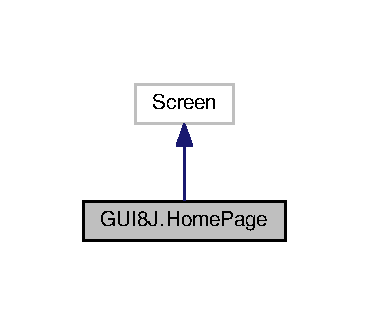
\includegraphics[width=177pt]{classGUI8J_1_1HomePage__inherit__graph}
\end{center}
\end{figure}


Collaboration diagram for G\+U\+I8\+J.\+Home\+Page\+:
\nopagebreak
\begin{figure}[H]
\begin{center}
\leavevmode
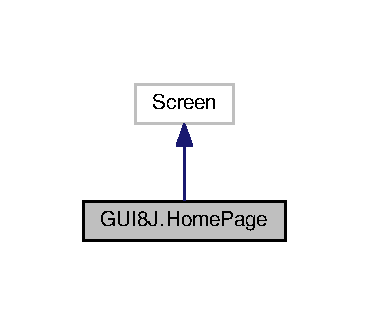
\includegraphics[width=177pt]{classGUI8J_1_1HomePage__coll__graph}
\end{center}
\end{figure}


The documentation for this class was generated from the following file\+:\begin{DoxyCompactItemize}
\item 
/home/jac0656/\+Desktop/\+J-\/\+O-\/\+R-\/\+G-\/\+E/\+U\+N\+T-\/\+N\+A\+S\+A/\+G\+U\+I/\hyperlink{GUI8J_8py}{G\+U\+I8\+J.\+py}\end{DoxyCompactItemize}

\hypertarget{classTestingGUI_1_1HomePage}{}\section{Testing\+G\+U\+I.\+Home\+Page Class Reference}
\label{classTestingGUI_1_1HomePage}\index{Testing\+G\+U\+I.\+Home\+Page@{Testing\+G\+U\+I.\+Home\+Page}}


Inheritance diagram for Testing\+G\+U\+I.\+Home\+Page\+:
\nopagebreak
\begin{figure}[H]
\begin{center}
\leavevmode
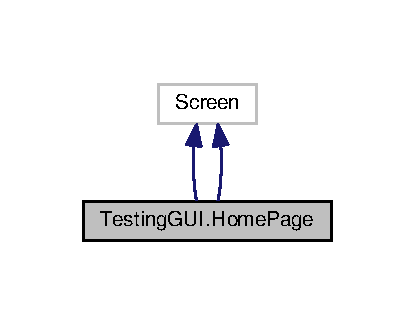
\includegraphics[width=199pt]{classTestingGUI_1_1HomePage__inherit__graph}
\end{center}
\end{figure}


Collaboration diagram for Testing\+G\+U\+I.\+Home\+Page\+:
\nopagebreak
\begin{figure}[H]
\begin{center}
\leavevmode
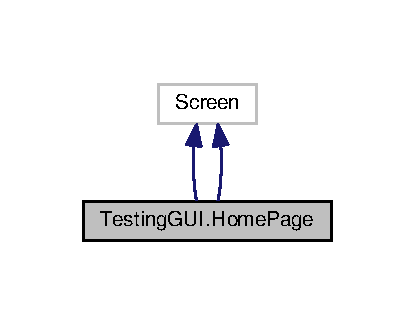
\includegraphics[width=199pt]{classTestingGUI_1_1HomePage__coll__graph}
\end{center}
\end{figure}


The documentation for this class was generated from the following file\+:\begin{DoxyCompactItemize}
\item 
/home/jac0656/\+Desktop/\+J-\/\+O-\/\+R-\/\+G-\/\+E/\+U\+N\+T-\/\+N\+A\+S\+A/\+G\+U\+I/\hyperlink{GUI_2TestingGUI_8py}{Testing\+G\+U\+I.\+py}\end{DoxyCompactItemize}

\hypertarget{classGUI8-5pm_1_1HomePage}{}\section{G\+U\+I8-\/5pm.Home\+Page Class Reference}
\label{classGUI8-5pm_1_1HomePage}\index{G\+U\+I8-\/5pm.\+Home\+Page@{G\+U\+I8-\/5pm.\+Home\+Page}}


Inheritance diagram for G\+U\+I8-\/5pm.Home\+Page\+:\nopagebreak
\begin{figure}[H]
\begin{center}
\leavevmode
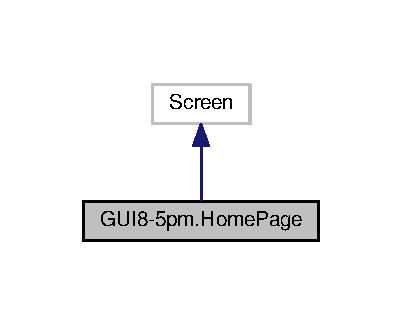
\includegraphics[width=193pt]{classGUI8-5pm_1_1HomePage__inherit__graph}
\end{center}
\end{figure}


Collaboration diagram for G\+U\+I8-\/5pm.Home\+Page\+:\nopagebreak
\begin{figure}[H]
\begin{center}
\leavevmode
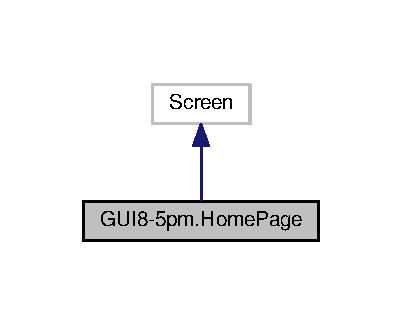
\includegraphics[width=193pt]{classGUI8-5pm_1_1HomePage__coll__graph}
\end{center}
\end{figure}
\subsection*{Public Member Functions}
\begin{DoxyCompactItemize}
\item 
def \hyperlink{classGUI8-5pm_1_1HomePage_a0f5b74437a5335f042b84f979131276a}{verify} (self)
\item 
def \hyperlink{classGUI8-5pm_1_1HomePage_ab49e98b3b43f3bef65b02fc2d067f616}{check\+\_\+credentials} (self, arg1)
\end{DoxyCompactItemize}
\subsection*{Public Attributes}
\begin{DoxyCompactItemize}
\item 
\hyperlink{classGUI8-5pm_1_1HomePage_ace0000b1905ef123db0ffb0f7712ae43}{textuser}
\item 
\hyperlink{classGUI8-5pm_1_1HomePage_a9d8ee437ded9432047e0541bc9c38bbd}{textpass}
\end{DoxyCompactItemize}


\subsection{Member Function Documentation}
\index{G\+U\+I8-\/5pm\+::\+Home\+Page@{G\+U\+I8-\/5pm\+::\+Home\+Page}!check\+\_\+credentials@{check\+\_\+credentials}}
\index{check\+\_\+credentials@{check\+\_\+credentials}!G\+U\+I8-\/5pm\+::\+Home\+Page@{G\+U\+I8-\/5pm\+::\+Home\+Page}}
\subsubsection[{\texorpdfstring{check\+\_\+credentials(self, arg1)}{check_credentials(self, arg1)}}]{\setlength{\rightskip}{0pt plus 5cm}def G\+U\+I8-\/5pm.\+Home\+Page.\+check\+\_\+credentials (
\begin{DoxyParamCaption}
\item[{}]{self, }
\item[{}]{arg1}
\end{DoxyParamCaption}
)}\hypertarget{classGUI8-5pm_1_1HomePage_ab49e98b3b43f3bef65b02fc2d067f616}{}\label{classGUI8-5pm_1_1HomePage_ab49e98b3b43f3bef65b02fc2d067f616}
\index{G\+U\+I8-\/5pm\+::\+Home\+Page@{G\+U\+I8-\/5pm\+::\+Home\+Page}!verify@{verify}}
\index{verify@{verify}!G\+U\+I8-\/5pm\+::\+Home\+Page@{G\+U\+I8-\/5pm\+::\+Home\+Page}}
\subsubsection[{\texorpdfstring{verify(self)}{verify(self)}}]{\setlength{\rightskip}{0pt plus 5cm}def G\+U\+I8-\/5pm.\+Home\+Page.\+verify (
\begin{DoxyParamCaption}
\item[{}]{self}
\end{DoxyParamCaption}
)}\hypertarget{classGUI8-5pm_1_1HomePage_a0f5b74437a5335f042b84f979131276a}{}\label{classGUI8-5pm_1_1HomePage_a0f5b74437a5335f042b84f979131276a}


\subsection{Member Data Documentation}
\index{G\+U\+I8-\/5pm\+::\+Home\+Page@{G\+U\+I8-\/5pm\+::\+Home\+Page}!textpass@{textpass}}
\index{textpass@{textpass}!G\+U\+I8-\/5pm\+::\+Home\+Page@{G\+U\+I8-\/5pm\+::\+Home\+Page}}
\subsubsection[{\texorpdfstring{textpass}{textpass}}]{\setlength{\rightskip}{0pt plus 5cm}G\+U\+I8-\/5pm.\+Home\+Page.\+textpass}\hypertarget{classGUI8-5pm_1_1HomePage_a9d8ee437ded9432047e0541bc9c38bbd}{}\label{classGUI8-5pm_1_1HomePage_a9d8ee437ded9432047e0541bc9c38bbd}
\index{G\+U\+I8-\/5pm\+::\+Home\+Page@{G\+U\+I8-\/5pm\+::\+Home\+Page}!textuser@{textuser}}
\index{textuser@{textuser}!G\+U\+I8-\/5pm\+::\+Home\+Page@{G\+U\+I8-\/5pm\+::\+Home\+Page}}
\subsubsection[{\texorpdfstring{textuser}{textuser}}]{\setlength{\rightskip}{0pt plus 5cm}G\+U\+I8-\/5pm.\+Home\+Page.\+textuser}\hypertarget{classGUI8-5pm_1_1HomePage_ace0000b1905ef123db0ffb0f7712ae43}{}\label{classGUI8-5pm_1_1HomePage_ace0000b1905ef123db0ffb0f7712ae43}


The documentation for this class was generated from the following file\+:\begin{DoxyCompactItemize}
\item 
/home/jac0656/\+Desktop/\+J-\/\+O-\/\+R-\/\+G-\/\+E/\+U\+N\+T-\/\+N\+A\+S\+A/\hyperlink{GUI8-5pm_8py}{G\+U\+I8-\/5pm.\+py}\end{DoxyCompactItemize}

\hypertarget{classsnowboydecoder_1_1HotwordDetector}{}\section{snowboydecoder.\+Hotword\+Detector Class Reference}
\label{classsnowboydecoder_1_1HotwordDetector}\index{snowboydecoder.\+Hotword\+Detector@{snowboydecoder.\+Hotword\+Detector}}


Inheritance diagram for snowboydecoder.\+Hotword\+Detector\+:
% FIG 0


Collaboration diagram for snowboydecoder.\+Hotword\+Detector\+:
% FIG 1
\subsection*{Public Member Functions}
\begin{DoxyCompactItemize}
\item 
def \hyperlink{classsnowboydecoder_1_1HotwordDetector_a22091f02a8fea2f6065f8bc45addf7fc}{\+\_\+\+\_\+init\+\_\+\+\_\+} (self, decoder\+\_\+model, resource=\hyperlink{namespacesnowboydecoder_ae9aa648d909800942df02cc34b56b83a}{R\+E\+S\+O\+U\+R\+C\+E\+\_\+\+F\+I\+LE}, sensitivity=\mbox{[}$\,$\mbox{]}, audio\+\_\+gain=1)
\item 
def \hyperlink{classsnowboydecoder_1_1HotwordDetector_a0b753c51c1a02be091a7673870cd74e6}{start} (self, detected\+\_\+callback=\hyperlink{namespacesnowboydecoder_a828506a06fcca3526430747208f904aa}{play\+\_\+audio\+\_\+file}, interrupt\+\_\+check=lambda\+:\+False, sleep\+\_\+time=0.\+03)
\item 
def \hyperlink{classsnowboydecoder_1_1HotwordDetector_a1ab6e303be1e4dbd5adaa9b9d29dfa1a}{terminate} (self)
\end{DoxyCompactItemize}
\subsection*{Public Attributes}
\begin{DoxyCompactItemize}
\item 
\hyperlink{classsnowboydecoder_1_1HotwordDetector_a443f1b4a74ff9e6dab682d9161b7aa52}{detector}
\item 
\hyperlink{classsnowboydecoder_1_1HotwordDetector_a45759e8fb8047abaf3697071cb88364c}{num\+\_\+hotwords}
\item 
\hyperlink{classsnowboydecoder_1_1HotwordDetector_ae5f5881d045e26f9e750b5e03c99f29c}{ring\+\_\+buffer}
\item 
\hyperlink{classsnowboydecoder_1_1HotwordDetector_a747f6301374f25541183bd2b7f0baac6}{audio}
\item 
\hyperlink{classsnowboydecoder_1_1HotwordDetector_a2658be70bb0b1939517e24f008d392a2}{stream\+\_\+in}
\end{DoxyCompactItemize}


\subsection{Constructor \& Destructor Documentation}
\mbox{\Hypertarget{classsnowboydecoder_1_1HotwordDetector_a22091f02a8fea2f6065f8bc45addf7fc}\label{classsnowboydecoder_1_1HotwordDetector_a22091f02a8fea2f6065f8bc45addf7fc}} 
\index{snowboydecoder\+::\+Hotword\+Detector@{snowboydecoder\+::\+Hotword\+Detector}!\+\_\+\+\_\+init\+\_\+\+\_\+@{\+\_\+\+\_\+init\+\_\+\+\_\+}}
\index{\+\_\+\+\_\+init\+\_\+\+\_\+@{\+\_\+\+\_\+init\+\_\+\+\_\+}!snowboydecoder\+::\+Hotword\+Detector@{snowboydecoder\+::\+Hotword\+Detector}}
\subsubsection{\texorpdfstring{\+\_\+\+\_\+init\+\_\+\+\_\+()}{\_\_init\_\_()}}
{\footnotesize\ttfamily def snowboydecoder.\+Hotword\+Detector.\+\_\+\+\_\+init\+\_\+\+\_\+ (\begin{DoxyParamCaption}\item[{}]{self,  }\item[{}]{decoder\+\_\+model,  }\item[{}]{resource = {\ttfamily \hyperlink{namespacesnowboydecoder_ae9aa648d909800942df02cc34b56b83a}{R\+E\+S\+O\+U\+R\+C\+E\+\_\+\+F\+I\+LE}},  }\item[{}]{sensitivity = {\ttfamily \mbox{[}\mbox{]}},  }\item[{}]{audio\+\_\+gain = {\ttfamily 1} }\end{DoxyParamCaption})}



\subsection{Member Function Documentation}
\mbox{\Hypertarget{classsnowboydecoder_1_1HotwordDetector_a0b753c51c1a02be091a7673870cd74e6}\label{classsnowboydecoder_1_1HotwordDetector_a0b753c51c1a02be091a7673870cd74e6}} 
\index{snowboydecoder\+::\+Hotword\+Detector@{snowboydecoder\+::\+Hotword\+Detector}!start@{start}}
\index{start@{start}!snowboydecoder\+::\+Hotword\+Detector@{snowboydecoder\+::\+Hotword\+Detector}}
\subsubsection{\texorpdfstring{start()}{start()}}
{\footnotesize\ttfamily def snowboydecoder.\+Hotword\+Detector.\+start (\begin{DoxyParamCaption}\item[{}]{self,  }\item[{}]{detected\+\_\+callback = {\ttfamily \hyperlink{namespacesnowboydecoder_a828506a06fcca3526430747208f904aa}{play\+\_\+audio\+\_\+file}},  }\item[{}]{interrupt\+\_\+check = {\ttfamily lambda\+:~False},  }\item[{}]{sleep\+\_\+time = {\ttfamily 0.03} }\end{DoxyParamCaption})}

\mbox{\Hypertarget{classsnowboydecoder_1_1HotwordDetector_a1ab6e303be1e4dbd5adaa9b9d29dfa1a}\label{classsnowboydecoder_1_1HotwordDetector_a1ab6e303be1e4dbd5adaa9b9d29dfa1a}} 
\index{snowboydecoder\+::\+Hotword\+Detector@{snowboydecoder\+::\+Hotword\+Detector}!terminate@{terminate}}
\index{terminate@{terminate}!snowboydecoder\+::\+Hotword\+Detector@{snowboydecoder\+::\+Hotword\+Detector}}
\subsubsection{\texorpdfstring{terminate()}{terminate()}}
{\footnotesize\ttfamily def snowboydecoder.\+Hotword\+Detector.\+terminate (\begin{DoxyParamCaption}\item[{}]{self }\end{DoxyParamCaption})}

\begin{DoxyVerb}Terminate audio stream. Users cannot call start() again to detect.
:return: None
\end{DoxyVerb}
 

\subsection{Member Data Documentation}
\mbox{\Hypertarget{classsnowboydecoder_1_1HotwordDetector_a747f6301374f25541183bd2b7f0baac6}\label{classsnowboydecoder_1_1HotwordDetector_a747f6301374f25541183bd2b7f0baac6}} 
\index{snowboydecoder\+::\+Hotword\+Detector@{snowboydecoder\+::\+Hotword\+Detector}!audio@{audio}}
\index{audio@{audio}!snowboydecoder\+::\+Hotword\+Detector@{snowboydecoder\+::\+Hotword\+Detector}}
\subsubsection{\texorpdfstring{audio}{audio}}
{\footnotesize\ttfamily snowboydecoder.\+Hotword\+Detector.\+audio}

\mbox{\Hypertarget{classsnowboydecoder_1_1HotwordDetector_a443f1b4a74ff9e6dab682d9161b7aa52}\label{classsnowboydecoder_1_1HotwordDetector_a443f1b4a74ff9e6dab682d9161b7aa52}} 
\index{snowboydecoder\+::\+Hotword\+Detector@{snowboydecoder\+::\+Hotword\+Detector}!detector@{detector}}
\index{detector@{detector}!snowboydecoder\+::\+Hotword\+Detector@{snowboydecoder\+::\+Hotword\+Detector}}
\subsubsection{\texorpdfstring{detector}{detector}}
{\footnotesize\ttfamily snowboydecoder.\+Hotword\+Detector.\+detector}

\mbox{\Hypertarget{classsnowboydecoder_1_1HotwordDetector_a45759e8fb8047abaf3697071cb88364c}\label{classsnowboydecoder_1_1HotwordDetector_a45759e8fb8047abaf3697071cb88364c}} 
\index{snowboydecoder\+::\+Hotword\+Detector@{snowboydecoder\+::\+Hotword\+Detector}!num\+\_\+hotwords@{num\+\_\+hotwords}}
\index{num\+\_\+hotwords@{num\+\_\+hotwords}!snowboydecoder\+::\+Hotword\+Detector@{snowboydecoder\+::\+Hotword\+Detector}}
\subsubsection{\texorpdfstring{num\+\_\+hotwords}{num\_hotwords}}
{\footnotesize\ttfamily snowboydecoder.\+Hotword\+Detector.\+num\+\_\+hotwords}

\mbox{\Hypertarget{classsnowboydecoder_1_1HotwordDetector_ae5f5881d045e26f9e750b5e03c99f29c}\label{classsnowboydecoder_1_1HotwordDetector_ae5f5881d045e26f9e750b5e03c99f29c}} 
\index{snowboydecoder\+::\+Hotword\+Detector@{snowboydecoder\+::\+Hotword\+Detector}!ring\+\_\+buffer@{ring\+\_\+buffer}}
\index{ring\+\_\+buffer@{ring\+\_\+buffer}!snowboydecoder\+::\+Hotword\+Detector@{snowboydecoder\+::\+Hotword\+Detector}}
\subsubsection{\texorpdfstring{ring\+\_\+buffer}{ring\_buffer}}
{\footnotesize\ttfamily snowboydecoder.\+Hotword\+Detector.\+ring\+\_\+buffer}

\mbox{\Hypertarget{classsnowboydecoder_1_1HotwordDetector_a2658be70bb0b1939517e24f008d392a2}\label{classsnowboydecoder_1_1HotwordDetector_a2658be70bb0b1939517e24f008d392a2}} 
\index{snowboydecoder\+::\+Hotword\+Detector@{snowboydecoder\+::\+Hotword\+Detector}!stream\+\_\+in@{stream\+\_\+in}}
\index{stream\+\_\+in@{stream\+\_\+in}!snowboydecoder\+::\+Hotword\+Detector@{snowboydecoder\+::\+Hotword\+Detector}}
\subsubsection{\texorpdfstring{stream\+\_\+in}{stream\_in}}
{\footnotesize\ttfamily snowboydecoder.\+Hotword\+Detector.\+stream\+\_\+in}



The documentation for this class was generated from the following file\+:\begin{DoxyCompactItemize}
\item 
/home/pi/\+Desktop/\+U\+N\+T-\/\+N\+A\+S\+A/voice\+O\+L\+A/\hyperlink{snowboydecoder_8py}{snowboydecoder.\+py}\end{DoxyCompactItemize}

\hypertarget{classGUI8J_1_1LightsView}{}\section{G\+U\+I8\+J.\+Lights\+View Class Reference}
\label{classGUI8J_1_1LightsView}\index{G\+U\+I8\+J.\+Lights\+View@{G\+U\+I8\+J.\+Lights\+View}}


Inheritance diagram for G\+U\+I8\+J.\+Lights\+View\+:
\nopagebreak
\begin{figure}[H]
\begin{center}
\leavevmode
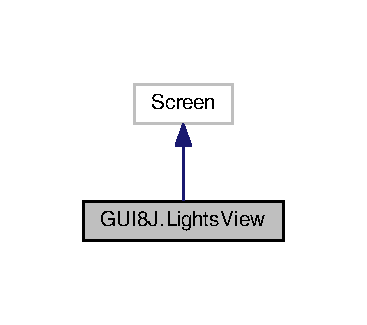
\includegraphics[width=176pt]{classGUI8J_1_1LightsView__inherit__graph}
\end{center}
\end{figure}


Collaboration diagram for G\+U\+I8\+J.\+Lights\+View\+:
\nopagebreak
\begin{figure}[H]
\begin{center}
\leavevmode
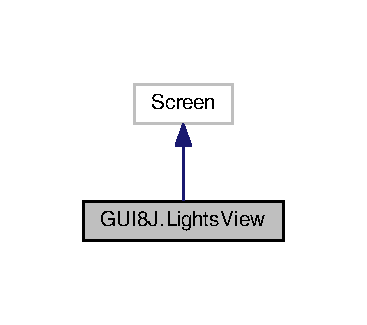
\includegraphics[width=176pt]{classGUI8J_1_1LightsView__coll__graph}
\end{center}
\end{figure}
\subsection*{Public Member Functions}
\begin{DoxyCompactItemize}
\item 
def \hyperlink{classGUI8J_1_1LightsView_aa869b90f2eb911a68ef3e77eb3a6a82a}{\+\_\+\+\_\+init\+\_\+\+\_\+} (self, kwargs)
\item 
def \hyperlink{classGUI8J_1_1LightsView_a92d033a19bdb2038412ea15f49edf535}{buildlist} (self)
\item 
def \hyperlink{classGUI8J_1_1LightsView_a5ce2e25c5856187c98420e319c5fca7f}{add\+\_\+room} (self)
\item 
def \hyperlink{classGUI8J_1_1LightsView_ad6ba3cded3ba2e6bf1da130625544a5c}{lightscallback} (self, instance, value)
\item 
def \hyperlink{classGUI8J_1_1LightsView_a45a9730f55978a8fc4c452dfa583332d}{callback} (self, instance, value)
\item 
def \hyperlink{classGUI8J_1_1LightsView_ac3ed1b51f74c502b2fd9ad7c36d3dcbd}{add\+\_\+to\+\_\+room} (self)
\item 
def \hyperlink{classGUI8J_1_1LightsView_ac4e2881bc3e4ce75ddf8b1937722974e}{room\+\_\+popup} (self)
\item 
def \hyperlink{classGUI8J_1_1LightsView_a829d96000de9fe0044acd685e005af0d}{store} (self, arg1)
\item 
def \hyperlink{classGUI8J_1_1LightsView_a6bb6e91505cef521592ecc5e231ca893}{update\+\_\+rooms} (self)
\item 
def \hyperlink{classGUI8J_1_1LightsView_addfb70b9f5e33de1f69d5b8880ad741f}{remove\+\_\+room} (self)
\item 
def \hyperlink{classGUI8J_1_1LightsView_a1a3f0a8522cfbe99e38330c862bacbad}{remove\+\_\+light} (self)
\end{DoxyCompactItemize}
\subsection*{Public Attributes}
\begin{DoxyCompactItemize}
\item 
\hyperlink{classGUI8J_1_1LightsView_ae46a41876c688b387ead511b3bf4e780}{textinput}
\end{DoxyCompactItemize}


\subsection{Constructor \& Destructor Documentation}
\index{G\+U\+I8\+J\+::\+Lights\+View@{G\+U\+I8\+J\+::\+Lights\+View}!\+\_\+\+\_\+init\+\_\+\+\_\+@{\+\_\+\+\_\+init\+\_\+\+\_\+}}
\index{\+\_\+\+\_\+init\+\_\+\+\_\+@{\+\_\+\+\_\+init\+\_\+\+\_\+}!G\+U\+I8\+J\+::\+Lights\+View@{G\+U\+I8\+J\+::\+Lights\+View}}
\subsubsection[{\texorpdfstring{\+\_\+\+\_\+init\+\_\+\+\_\+(self, kwargs)}{__init__(self, kwargs)}}]{\setlength{\rightskip}{0pt plus 5cm}def G\+U\+I8\+J.\+Lights\+View.\+\_\+\+\_\+init\+\_\+\+\_\+ (
\begin{DoxyParamCaption}
\item[{}]{self, }
\item[{}]{kwargs}
\end{DoxyParamCaption}
)}\hypertarget{classGUI8J_1_1LightsView_aa869b90f2eb911a68ef3e77eb3a6a82a}{}\label{classGUI8J_1_1LightsView_aa869b90f2eb911a68ef3e77eb3a6a82a}


\subsection{Member Function Documentation}
\index{G\+U\+I8\+J\+::\+Lights\+View@{G\+U\+I8\+J\+::\+Lights\+View}!add\+\_\+room@{add\+\_\+room}}
\index{add\+\_\+room@{add\+\_\+room}!G\+U\+I8\+J\+::\+Lights\+View@{G\+U\+I8\+J\+::\+Lights\+View}}
\subsubsection[{\texorpdfstring{add\+\_\+room(self)}{add_room(self)}}]{\setlength{\rightskip}{0pt plus 5cm}def G\+U\+I8\+J.\+Lights\+View.\+add\+\_\+room (
\begin{DoxyParamCaption}
\item[{}]{self}
\end{DoxyParamCaption}
)}\hypertarget{classGUI8J_1_1LightsView_a5ce2e25c5856187c98420e319c5fca7f}{}\label{classGUI8J_1_1LightsView_a5ce2e25c5856187c98420e319c5fca7f}
\index{G\+U\+I8\+J\+::\+Lights\+View@{G\+U\+I8\+J\+::\+Lights\+View}!add\+\_\+to\+\_\+room@{add\+\_\+to\+\_\+room}}
\index{add\+\_\+to\+\_\+room@{add\+\_\+to\+\_\+room}!G\+U\+I8\+J\+::\+Lights\+View@{G\+U\+I8\+J\+::\+Lights\+View}}
\subsubsection[{\texorpdfstring{add\+\_\+to\+\_\+room(self)}{add_to_room(self)}}]{\setlength{\rightskip}{0pt plus 5cm}def G\+U\+I8\+J.\+Lights\+View.\+add\+\_\+to\+\_\+room (
\begin{DoxyParamCaption}
\item[{}]{self}
\end{DoxyParamCaption}
)}\hypertarget{classGUI8J_1_1LightsView_ac3ed1b51f74c502b2fd9ad7c36d3dcbd}{}\label{classGUI8J_1_1LightsView_ac3ed1b51f74c502b2fd9ad7c36d3dcbd}
\index{G\+U\+I8\+J\+::\+Lights\+View@{G\+U\+I8\+J\+::\+Lights\+View}!buildlist@{buildlist}}
\index{buildlist@{buildlist}!G\+U\+I8\+J\+::\+Lights\+View@{G\+U\+I8\+J\+::\+Lights\+View}}
\subsubsection[{\texorpdfstring{buildlist(self)}{buildlist(self)}}]{\setlength{\rightskip}{0pt plus 5cm}def G\+U\+I8\+J.\+Lights\+View.\+buildlist (
\begin{DoxyParamCaption}
\item[{}]{self}
\end{DoxyParamCaption}
)}\hypertarget{classGUI8J_1_1LightsView_a92d033a19bdb2038412ea15f49edf535}{}\label{classGUI8J_1_1LightsView_a92d033a19bdb2038412ea15f49edf535}
\index{G\+U\+I8\+J\+::\+Lights\+View@{G\+U\+I8\+J\+::\+Lights\+View}!callback@{callback}}
\index{callback@{callback}!G\+U\+I8\+J\+::\+Lights\+View@{G\+U\+I8\+J\+::\+Lights\+View}}
\subsubsection[{\texorpdfstring{callback(self, instance, value)}{callback(self, instance, value)}}]{\setlength{\rightskip}{0pt plus 5cm}def G\+U\+I8\+J.\+Lights\+View.\+callback (
\begin{DoxyParamCaption}
\item[{}]{self, }
\item[{}]{instance, }
\item[{}]{value}
\end{DoxyParamCaption}
)}\hypertarget{classGUI8J_1_1LightsView_a45a9730f55978a8fc4c452dfa583332d}{}\label{classGUI8J_1_1LightsView_a45a9730f55978a8fc4c452dfa583332d}
\index{G\+U\+I8\+J\+::\+Lights\+View@{G\+U\+I8\+J\+::\+Lights\+View}!lightscallback@{lightscallback}}
\index{lightscallback@{lightscallback}!G\+U\+I8\+J\+::\+Lights\+View@{G\+U\+I8\+J\+::\+Lights\+View}}
\subsubsection[{\texorpdfstring{lightscallback(self, instance, value)}{lightscallback(self, instance, value)}}]{\setlength{\rightskip}{0pt plus 5cm}def G\+U\+I8\+J.\+Lights\+View.\+lightscallback (
\begin{DoxyParamCaption}
\item[{}]{self, }
\item[{}]{instance, }
\item[{}]{value}
\end{DoxyParamCaption}
)}\hypertarget{classGUI8J_1_1LightsView_ad6ba3cded3ba2e6bf1da130625544a5c}{}\label{classGUI8J_1_1LightsView_ad6ba3cded3ba2e6bf1da130625544a5c}
\index{G\+U\+I8\+J\+::\+Lights\+View@{G\+U\+I8\+J\+::\+Lights\+View}!remove\+\_\+light@{remove\+\_\+light}}
\index{remove\+\_\+light@{remove\+\_\+light}!G\+U\+I8\+J\+::\+Lights\+View@{G\+U\+I8\+J\+::\+Lights\+View}}
\subsubsection[{\texorpdfstring{remove\+\_\+light(self)}{remove_light(self)}}]{\setlength{\rightskip}{0pt plus 5cm}def G\+U\+I8\+J.\+Lights\+View.\+remove\+\_\+light (
\begin{DoxyParamCaption}
\item[{}]{self}
\end{DoxyParamCaption}
)}\hypertarget{classGUI8J_1_1LightsView_a1a3f0a8522cfbe99e38330c862bacbad}{}\label{classGUI8J_1_1LightsView_a1a3f0a8522cfbe99e38330c862bacbad}
\index{G\+U\+I8\+J\+::\+Lights\+View@{G\+U\+I8\+J\+::\+Lights\+View}!remove\+\_\+room@{remove\+\_\+room}}
\index{remove\+\_\+room@{remove\+\_\+room}!G\+U\+I8\+J\+::\+Lights\+View@{G\+U\+I8\+J\+::\+Lights\+View}}
\subsubsection[{\texorpdfstring{remove\+\_\+room(self)}{remove_room(self)}}]{\setlength{\rightskip}{0pt plus 5cm}def G\+U\+I8\+J.\+Lights\+View.\+remove\+\_\+room (
\begin{DoxyParamCaption}
\item[{}]{self}
\end{DoxyParamCaption}
)}\hypertarget{classGUI8J_1_1LightsView_addfb70b9f5e33de1f69d5b8880ad741f}{}\label{classGUI8J_1_1LightsView_addfb70b9f5e33de1f69d5b8880ad741f}
\index{G\+U\+I8\+J\+::\+Lights\+View@{G\+U\+I8\+J\+::\+Lights\+View}!room\+\_\+popup@{room\+\_\+popup}}
\index{room\+\_\+popup@{room\+\_\+popup}!G\+U\+I8\+J\+::\+Lights\+View@{G\+U\+I8\+J\+::\+Lights\+View}}
\subsubsection[{\texorpdfstring{room\+\_\+popup(self)}{room_popup(self)}}]{\setlength{\rightskip}{0pt plus 5cm}def G\+U\+I8\+J.\+Lights\+View.\+room\+\_\+popup (
\begin{DoxyParamCaption}
\item[{}]{self}
\end{DoxyParamCaption}
)}\hypertarget{classGUI8J_1_1LightsView_ac4e2881bc3e4ce75ddf8b1937722974e}{}\label{classGUI8J_1_1LightsView_ac4e2881bc3e4ce75ddf8b1937722974e}
\index{G\+U\+I8\+J\+::\+Lights\+View@{G\+U\+I8\+J\+::\+Lights\+View}!store@{store}}
\index{store@{store}!G\+U\+I8\+J\+::\+Lights\+View@{G\+U\+I8\+J\+::\+Lights\+View}}
\subsubsection[{\texorpdfstring{store(self, arg1)}{store(self, arg1)}}]{\setlength{\rightskip}{0pt plus 5cm}def G\+U\+I8\+J.\+Lights\+View.\+store (
\begin{DoxyParamCaption}
\item[{}]{self, }
\item[{}]{arg1}
\end{DoxyParamCaption}
)}\hypertarget{classGUI8J_1_1LightsView_a829d96000de9fe0044acd685e005af0d}{}\label{classGUI8J_1_1LightsView_a829d96000de9fe0044acd685e005af0d}
\index{G\+U\+I8\+J\+::\+Lights\+View@{G\+U\+I8\+J\+::\+Lights\+View}!update\+\_\+rooms@{update\+\_\+rooms}}
\index{update\+\_\+rooms@{update\+\_\+rooms}!G\+U\+I8\+J\+::\+Lights\+View@{G\+U\+I8\+J\+::\+Lights\+View}}
\subsubsection[{\texorpdfstring{update\+\_\+rooms(self)}{update_rooms(self)}}]{\setlength{\rightskip}{0pt plus 5cm}def G\+U\+I8\+J.\+Lights\+View.\+update\+\_\+rooms (
\begin{DoxyParamCaption}
\item[{}]{self}
\end{DoxyParamCaption}
)}\hypertarget{classGUI8J_1_1LightsView_a6bb6e91505cef521592ecc5e231ca893}{}\label{classGUI8J_1_1LightsView_a6bb6e91505cef521592ecc5e231ca893}


\subsection{Member Data Documentation}
\index{G\+U\+I8\+J\+::\+Lights\+View@{G\+U\+I8\+J\+::\+Lights\+View}!textinput@{textinput}}
\index{textinput@{textinput}!G\+U\+I8\+J\+::\+Lights\+View@{G\+U\+I8\+J\+::\+Lights\+View}}
\subsubsection[{\texorpdfstring{textinput}{textinput}}]{\setlength{\rightskip}{0pt plus 5cm}G\+U\+I8\+J.\+Lights\+View.\+textinput}\hypertarget{classGUI8J_1_1LightsView_ae46a41876c688b387ead511b3bf4e780}{}\label{classGUI8J_1_1LightsView_ae46a41876c688b387ead511b3bf4e780}


The documentation for this class was generated from the following file\+:\begin{DoxyCompactItemize}
\item 
/home/jac0656/\+Desktop/\+J-\/\+O-\/\+R-\/\+G-\/\+E/\+U\+N\+T-\/\+N\+A\+S\+A/\+G\+U\+I/\hyperlink{GUI8J_8py}{G\+U\+I8\+J.\+py}\end{DoxyCompactItemize}

\hypertarget{classTestingGUI_1_1LightsView}{}\section{Testing\+G\+U\+I.\+Lights\+View Class Reference}
\label{classTestingGUI_1_1LightsView}\index{Testing\+G\+U\+I.\+Lights\+View@{Testing\+G\+U\+I.\+Lights\+View}}


Inheritance diagram for Testing\+G\+U\+I.\+Lights\+View\+:
\nopagebreak
\begin{figure}[H]
\begin{center}
\leavevmode
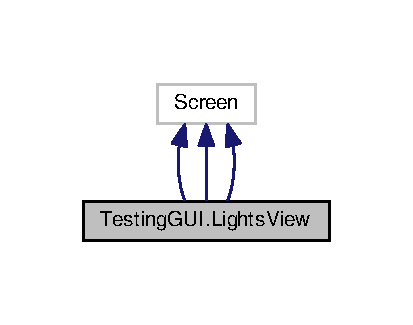
\includegraphics[width=198pt]{classTestingGUI_1_1LightsView__inherit__graph}
\end{center}
\end{figure}


Collaboration diagram for Testing\+G\+U\+I.\+Lights\+View\+:
\nopagebreak
\begin{figure}[H]
\begin{center}
\leavevmode
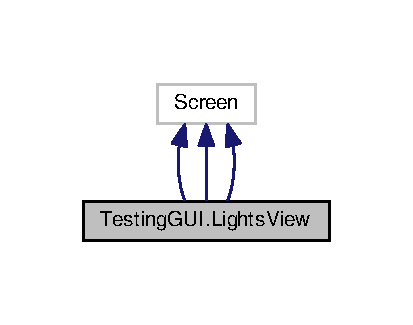
\includegraphics[width=198pt]{classTestingGUI_1_1LightsView__coll__graph}
\end{center}
\end{figure}
\subsection*{Public Member Functions}
\begin{DoxyCompactItemize}
\item 
def \hyperlink{classTestingGUI_1_1LightsView_ae63565dfb2328abb68fa8751284425a9}{\+\_\+\+\_\+init\+\_\+\+\_\+} (self, kwargs)
\item 
def \hyperlink{classTestingGUI_1_1LightsView_ad567fc119c87bdf050d2d105cffb102e}{buildlist} (self)
\item 
def \hyperlink{classTestingGUI_1_1LightsView_ae28189742abd26346c227385fe8866c7}{update} (self)
\item 
def \hyperlink{classTestingGUI_1_1LightsView_ab04e59790bba8440f9f1d65e84bc8ae6}{add\+\_\+room} (self)
\item 
def \hyperlink{classTestingGUI_1_1LightsView_abc44bd1d87c0d060890ad095b6195d27}{lightscallback} (self, instance, value)
\item 
def \hyperlink{classTestingGUI_1_1LightsView_a6868b6f77d43e03f6568b62169c9b19c}{callback} (self, instance, value)
\item 
def \hyperlink{classTestingGUI_1_1LightsView_a38460cbc7553198ef9a613d09919e077}{add\+\_\+to\+\_\+room} (self)
\item 
def \hyperlink{classTestingGUI_1_1LightsView_a3ff5b4674219060370bd91c84e99513c}{store\+\_\+lights\+\_\+assigned} (self, arg1)
\item 
def \hyperlink{classTestingGUI_1_1LightsView_ad2a97175fc114e694c6fe598361c6334}{move\+\_\+lights\+\_\+database} (self)
\item 
def \hyperlink{classTestingGUI_1_1LightsView_add6c257a4625658791c08aca275dbe4d}{update\+\_\+rooms} (self)
\item 
def \hyperlink{classTestingGUI_1_1LightsView_a363b48af2153effb586500f5ca0f371d}{write2\+J\+S\+ON} (self, dictionary)
\item 
def \hyperlink{classTestingGUI_1_1LightsView_a956aabd6c68ac0028a5dbc46ae9475ad}{store} (self, arg1)
\item 
def \hyperlink{classTestingGUI_1_1LightsView_a5f41c66493303b7174b335356d4deee5}{remove\+\_\+room} (self)
\item 
def \hyperlink{classTestingGUI_1_1LightsView_aa302b8817251a5f3c0f2c0d153073399}{remove\+\_\+light} (self)
\item 
def \hyperlink{classTestingGUI_1_1LightsView_ae63565dfb2328abb68fa8751284425a9}{\+\_\+\+\_\+init\+\_\+\+\_\+} (self, kwargs)
\item 
def \hyperlink{classTestingGUI_1_1LightsView_ad567fc119c87bdf050d2d105cffb102e}{buildlist} (self)
\item 
def \hyperlink{classTestingGUI_1_1LightsView_ae28189742abd26346c227385fe8866c7}{update} (self)
\item 
def \hyperlink{classTestingGUI_1_1LightsView_ab04e59790bba8440f9f1d65e84bc8ae6}{add\+\_\+room} (self)
\item 
def \hyperlink{classTestingGUI_1_1LightsView_abc44bd1d87c0d060890ad095b6195d27}{lightscallback} (self, instance, value)
\item 
def \hyperlink{classTestingGUI_1_1LightsView_a6868b6f77d43e03f6568b62169c9b19c}{callback} (self, instance, value)
\item 
def \hyperlink{classTestingGUI_1_1LightsView_a38460cbc7553198ef9a613d09919e077}{add\+\_\+to\+\_\+room} (self)
\item 
def \hyperlink{classTestingGUI_1_1LightsView_a3ff5b4674219060370bd91c84e99513c}{store\+\_\+lights\+\_\+assigned} (self, arg1)
\item 
def \hyperlink{classTestingGUI_1_1LightsView_ad2a97175fc114e694c6fe598361c6334}{move\+\_\+lights\+\_\+database} (self)
\item 
def \hyperlink{classTestingGUI_1_1LightsView_add6c257a4625658791c08aca275dbe4d}{update\+\_\+rooms} (self)
\item 
def \hyperlink{classTestingGUI_1_1LightsView_a363b48af2153effb586500f5ca0f371d}{write2\+J\+S\+ON} (self, dictionary)
\item 
def \hyperlink{classTestingGUI_1_1LightsView_a956aabd6c68ac0028a5dbc46ae9475ad}{store} (self, arg1)
\item 
def \hyperlink{classTestingGUI_1_1LightsView_a5f41c66493303b7174b335356d4deee5}{remove\+\_\+room} (self)
\item 
def \hyperlink{classTestingGUI_1_1LightsView_aa302b8817251a5f3c0f2c0d153073399}{remove\+\_\+light} (self)
\end{DoxyCompactItemize}
\subsection*{Public Attributes}
\begin{DoxyCompactItemize}
\item 
\hyperlink{classTestingGUI_1_1LightsView_aa809676a8370b352332b15861fac843e}{textinput}
\end{DoxyCompactItemize}


\subsection{Constructor \& Destructor Documentation}
\index{Testing\+G\+U\+I\+::\+Lights\+View@{Testing\+G\+U\+I\+::\+Lights\+View}!\+\_\+\+\_\+init\+\_\+\+\_\+@{\+\_\+\+\_\+init\+\_\+\+\_\+}}
\index{\+\_\+\+\_\+init\+\_\+\+\_\+@{\+\_\+\+\_\+init\+\_\+\+\_\+}!Testing\+G\+U\+I\+::\+Lights\+View@{Testing\+G\+U\+I\+::\+Lights\+View}}
\subsubsection[{\texorpdfstring{\+\_\+\+\_\+init\+\_\+\+\_\+(self, kwargs)}{__init__(self, kwargs)}}]{\setlength{\rightskip}{0pt plus 5cm}def Testing\+G\+U\+I.\+Lights\+View.\+\_\+\+\_\+init\+\_\+\+\_\+ (
\begin{DoxyParamCaption}
\item[{}]{self, }
\item[{}]{kwargs}
\end{DoxyParamCaption}
)}\hypertarget{classTestingGUI_1_1LightsView_ae63565dfb2328abb68fa8751284425a9}{}\label{classTestingGUI_1_1LightsView_ae63565dfb2328abb68fa8751284425a9}
\index{Testing\+G\+U\+I\+::\+Lights\+View@{Testing\+G\+U\+I\+::\+Lights\+View}!\+\_\+\+\_\+init\+\_\+\+\_\+@{\+\_\+\+\_\+init\+\_\+\+\_\+}}
\index{\+\_\+\+\_\+init\+\_\+\+\_\+@{\+\_\+\+\_\+init\+\_\+\+\_\+}!Testing\+G\+U\+I\+::\+Lights\+View@{Testing\+G\+U\+I\+::\+Lights\+View}}
\subsubsection[{\texorpdfstring{\+\_\+\+\_\+init\+\_\+\+\_\+(self, kwargs)}{__init__(self, kwargs)}}]{\setlength{\rightskip}{0pt plus 5cm}def Testing\+G\+U\+I.\+Lights\+View.\+\_\+\+\_\+init\+\_\+\+\_\+ (
\begin{DoxyParamCaption}
\item[{}]{self, }
\item[{}]{kwargs}
\end{DoxyParamCaption}
)}\hypertarget{classTestingGUI_1_1LightsView_ae63565dfb2328abb68fa8751284425a9}{}\label{classTestingGUI_1_1LightsView_ae63565dfb2328abb68fa8751284425a9}


\subsection{Member Function Documentation}
\index{Testing\+G\+U\+I\+::\+Lights\+View@{Testing\+G\+U\+I\+::\+Lights\+View}!add\+\_\+room@{add\+\_\+room}}
\index{add\+\_\+room@{add\+\_\+room}!Testing\+G\+U\+I\+::\+Lights\+View@{Testing\+G\+U\+I\+::\+Lights\+View}}
\subsubsection[{\texorpdfstring{add\+\_\+room(self)}{add_room(self)}}]{\setlength{\rightskip}{0pt plus 5cm}def Testing\+G\+U\+I.\+Lights\+View.\+add\+\_\+room (
\begin{DoxyParamCaption}
\item[{}]{self}
\end{DoxyParamCaption}
)}\hypertarget{classTestingGUI_1_1LightsView_ab04e59790bba8440f9f1d65e84bc8ae6}{}\label{classTestingGUI_1_1LightsView_ab04e59790bba8440f9f1d65e84bc8ae6}
\index{Testing\+G\+U\+I\+::\+Lights\+View@{Testing\+G\+U\+I\+::\+Lights\+View}!add\+\_\+room@{add\+\_\+room}}
\index{add\+\_\+room@{add\+\_\+room}!Testing\+G\+U\+I\+::\+Lights\+View@{Testing\+G\+U\+I\+::\+Lights\+View}}
\subsubsection[{\texorpdfstring{add\+\_\+room(self)}{add_room(self)}}]{\setlength{\rightskip}{0pt plus 5cm}def Testing\+G\+U\+I.\+Lights\+View.\+add\+\_\+room (
\begin{DoxyParamCaption}
\item[{}]{self}
\end{DoxyParamCaption}
)}\hypertarget{classTestingGUI_1_1LightsView_ab04e59790bba8440f9f1d65e84bc8ae6}{}\label{classTestingGUI_1_1LightsView_ab04e59790bba8440f9f1d65e84bc8ae6}
\index{Testing\+G\+U\+I\+::\+Lights\+View@{Testing\+G\+U\+I\+::\+Lights\+View}!add\+\_\+to\+\_\+room@{add\+\_\+to\+\_\+room}}
\index{add\+\_\+to\+\_\+room@{add\+\_\+to\+\_\+room}!Testing\+G\+U\+I\+::\+Lights\+View@{Testing\+G\+U\+I\+::\+Lights\+View}}
\subsubsection[{\texorpdfstring{add\+\_\+to\+\_\+room(self)}{add_to_room(self)}}]{\setlength{\rightskip}{0pt plus 5cm}def Testing\+G\+U\+I.\+Lights\+View.\+add\+\_\+to\+\_\+room (
\begin{DoxyParamCaption}
\item[{}]{self}
\end{DoxyParamCaption}
)}\hypertarget{classTestingGUI_1_1LightsView_a38460cbc7553198ef9a613d09919e077}{}\label{classTestingGUI_1_1LightsView_a38460cbc7553198ef9a613d09919e077}
\index{Testing\+G\+U\+I\+::\+Lights\+View@{Testing\+G\+U\+I\+::\+Lights\+View}!add\+\_\+to\+\_\+room@{add\+\_\+to\+\_\+room}}
\index{add\+\_\+to\+\_\+room@{add\+\_\+to\+\_\+room}!Testing\+G\+U\+I\+::\+Lights\+View@{Testing\+G\+U\+I\+::\+Lights\+View}}
\subsubsection[{\texorpdfstring{add\+\_\+to\+\_\+room(self)}{add_to_room(self)}}]{\setlength{\rightskip}{0pt plus 5cm}def Testing\+G\+U\+I.\+Lights\+View.\+add\+\_\+to\+\_\+room (
\begin{DoxyParamCaption}
\item[{}]{self}
\end{DoxyParamCaption}
)}\hypertarget{classTestingGUI_1_1LightsView_a38460cbc7553198ef9a613d09919e077}{}\label{classTestingGUI_1_1LightsView_a38460cbc7553198ef9a613d09919e077}
\index{Testing\+G\+U\+I\+::\+Lights\+View@{Testing\+G\+U\+I\+::\+Lights\+View}!buildlist@{buildlist}}
\index{buildlist@{buildlist}!Testing\+G\+U\+I\+::\+Lights\+View@{Testing\+G\+U\+I\+::\+Lights\+View}}
\subsubsection[{\texorpdfstring{buildlist(self)}{buildlist(self)}}]{\setlength{\rightskip}{0pt plus 5cm}def Testing\+G\+U\+I.\+Lights\+View.\+buildlist (
\begin{DoxyParamCaption}
\item[{}]{self}
\end{DoxyParamCaption}
)}\hypertarget{classTestingGUI_1_1LightsView_ad567fc119c87bdf050d2d105cffb102e}{}\label{classTestingGUI_1_1LightsView_ad567fc119c87bdf050d2d105cffb102e}
\index{Testing\+G\+U\+I\+::\+Lights\+View@{Testing\+G\+U\+I\+::\+Lights\+View}!buildlist@{buildlist}}
\index{buildlist@{buildlist}!Testing\+G\+U\+I\+::\+Lights\+View@{Testing\+G\+U\+I\+::\+Lights\+View}}
\subsubsection[{\texorpdfstring{buildlist(self)}{buildlist(self)}}]{\setlength{\rightskip}{0pt plus 5cm}def Testing\+G\+U\+I.\+Lights\+View.\+buildlist (
\begin{DoxyParamCaption}
\item[{}]{self}
\end{DoxyParamCaption}
)}\hypertarget{classTestingGUI_1_1LightsView_ad567fc119c87bdf050d2d105cffb102e}{}\label{classTestingGUI_1_1LightsView_ad567fc119c87bdf050d2d105cffb102e}
\index{Testing\+G\+U\+I\+::\+Lights\+View@{Testing\+G\+U\+I\+::\+Lights\+View}!callback@{callback}}
\index{callback@{callback}!Testing\+G\+U\+I\+::\+Lights\+View@{Testing\+G\+U\+I\+::\+Lights\+View}}
\subsubsection[{\texorpdfstring{callback(self, instance, value)}{callback(self, instance, value)}}]{\setlength{\rightskip}{0pt plus 5cm}def Testing\+G\+U\+I.\+Lights\+View.\+callback (
\begin{DoxyParamCaption}
\item[{}]{self, }
\item[{}]{instance, }
\item[{}]{value}
\end{DoxyParamCaption}
)}\hypertarget{classTestingGUI_1_1LightsView_a6868b6f77d43e03f6568b62169c9b19c}{}\label{classTestingGUI_1_1LightsView_a6868b6f77d43e03f6568b62169c9b19c}
\index{Testing\+G\+U\+I\+::\+Lights\+View@{Testing\+G\+U\+I\+::\+Lights\+View}!callback@{callback}}
\index{callback@{callback}!Testing\+G\+U\+I\+::\+Lights\+View@{Testing\+G\+U\+I\+::\+Lights\+View}}
\subsubsection[{\texorpdfstring{callback(self, instance, value)}{callback(self, instance, value)}}]{\setlength{\rightskip}{0pt plus 5cm}def Testing\+G\+U\+I.\+Lights\+View.\+callback (
\begin{DoxyParamCaption}
\item[{}]{self, }
\item[{}]{instance, }
\item[{}]{value}
\end{DoxyParamCaption}
)}\hypertarget{classTestingGUI_1_1LightsView_a6868b6f77d43e03f6568b62169c9b19c}{}\label{classTestingGUI_1_1LightsView_a6868b6f77d43e03f6568b62169c9b19c}
\index{Testing\+G\+U\+I\+::\+Lights\+View@{Testing\+G\+U\+I\+::\+Lights\+View}!lightscallback@{lightscallback}}
\index{lightscallback@{lightscallback}!Testing\+G\+U\+I\+::\+Lights\+View@{Testing\+G\+U\+I\+::\+Lights\+View}}
\subsubsection[{\texorpdfstring{lightscallback(self, instance, value)}{lightscallback(self, instance, value)}}]{\setlength{\rightskip}{0pt plus 5cm}def Testing\+G\+U\+I.\+Lights\+View.\+lightscallback (
\begin{DoxyParamCaption}
\item[{}]{self, }
\item[{}]{instance, }
\item[{}]{value}
\end{DoxyParamCaption}
)}\hypertarget{classTestingGUI_1_1LightsView_abc44bd1d87c0d060890ad095b6195d27}{}\label{classTestingGUI_1_1LightsView_abc44bd1d87c0d060890ad095b6195d27}
\index{Testing\+G\+U\+I\+::\+Lights\+View@{Testing\+G\+U\+I\+::\+Lights\+View}!lightscallback@{lightscallback}}
\index{lightscallback@{lightscallback}!Testing\+G\+U\+I\+::\+Lights\+View@{Testing\+G\+U\+I\+::\+Lights\+View}}
\subsubsection[{\texorpdfstring{lightscallback(self, instance, value)}{lightscallback(self, instance, value)}}]{\setlength{\rightskip}{0pt plus 5cm}def Testing\+G\+U\+I.\+Lights\+View.\+lightscallback (
\begin{DoxyParamCaption}
\item[{}]{self, }
\item[{}]{instance, }
\item[{}]{value}
\end{DoxyParamCaption}
)}\hypertarget{classTestingGUI_1_1LightsView_abc44bd1d87c0d060890ad095b6195d27}{}\label{classTestingGUI_1_1LightsView_abc44bd1d87c0d060890ad095b6195d27}
\index{Testing\+G\+U\+I\+::\+Lights\+View@{Testing\+G\+U\+I\+::\+Lights\+View}!move\+\_\+lights\+\_\+database@{move\+\_\+lights\+\_\+database}}
\index{move\+\_\+lights\+\_\+database@{move\+\_\+lights\+\_\+database}!Testing\+G\+U\+I\+::\+Lights\+View@{Testing\+G\+U\+I\+::\+Lights\+View}}
\subsubsection[{\texorpdfstring{move\+\_\+lights\+\_\+database(self)}{move_lights_database(self)}}]{\setlength{\rightskip}{0pt plus 5cm}def Testing\+G\+U\+I.\+Lights\+View.\+move\+\_\+lights\+\_\+database (
\begin{DoxyParamCaption}
\item[{}]{self}
\end{DoxyParamCaption}
)}\hypertarget{classTestingGUI_1_1LightsView_ad2a97175fc114e694c6fe598361c6334}{}\label{classTestingGUI_1_1LightsView_ad2a97175fc114e694c6fe598361c6334}
\index{Testing\+G\+U\+I\+::\+Lights\+View@{Testing\+G\+U\+I\+::\+Lights\+View}!move\+\_\+lights\+\_\+database@{move\+\_\+lights\+\_\+database}}
\index{move\+\_\+lights\+\_\+database@{move\+\_\+lights\+\_\+database}!Testing\+G\+U\+I\+::\+Lights\+View@{Testing\+G\+U\+I\+::\+Lights\+View}}
\subsubsection[{\texorpdfstring{move\+\_\+lights\+\_\+database(self)}{move_lights_database(self)}}]{\setlength{\rightskip}{0pt plus 5cm}def Testing\+G\+U\+I.\+Lights\+View.\+move\+\_\+lights\+\_\+database (
\begin{DoxyParamCaption}
\item[{}]{self}
\end{DoxyParamCaption}
)}\hypertarget{classTestingGUI_1_1LightsView_ad2a97175fc114e694c6fe598361c6334}{}\label{classTestingGUI_1_1LightsView_ad2a97175fc114e694c6fe598361c6334}
\index{Testing\+G\+U\+I\+::\+Lights\+View@{Testing\+G\+U\+I\+::\+Lights\+View}!remove\+\_\+light@{remove\+\_\+light}}
\index{remove\+\_\+light@{remove\+\_\+light}!Testing\+G\+U\+I\+::\+Lights\+View@{Testing\+G\+U\+I\+::\+Lights\+View}}
\subsubsection[{\texorpdfstring{remove\+\_\+light(self)}{remove_light(self)}}]{\setlength{\rightskip}{0pt plus 5cm}def Testing\+G\+U\+I.\+Lights\+View.\+remove\+\_\+light (
\begin{DoxyParamCaption}
\item[{}]{self}
\end{DoxyParamCaption}
)}\hypertarget{classTestingGUI_1_1LightsView_aa302b8817251a5f3c0f2c0d153073399}{}\label{classTestingGUI_1_1LightsView_aa302b8817251a5f3c0f2c0d153073399}
\index{Testing\+G\+U\+I\+::\+Lights\+View@{Testing\+G\+U\+I\+::\+Lights\+View}!remove\+\_\+light@{remove\+\_\+light}}
\index{remove\+\_\+light@{remove\+\_\+light}!Testing\+G\+U\+I\+::\+Lights\+View@{Testing\+G\+U\+I\+::\+Lights\+View}}
\subsubsection[{\texorpdfstring{remove\+\_\+light(self)}{remove_light(self)}}]{\setlength{\rightskip}{0pt plus 5cm}def Testing\+G\+U\+I.\+Lights\+View.\+remove\+\_\+light (
\begin{DoxyParamCaption}
\item[{}]{self}
\end{DoxyParamCaption}
)}\hypertarget{classTestingGUI_1_1LightsView_aa302b8817251a5f3c0f2c0d153073399}{}\label{classTestingGUI_1_1LightsView_aa302b8817251a5f3c0f2c0d153073399}
\index{Testing\+G\+U\+I\+::\+Lights\+View@{Testing\+G\+U\+I\+::\+Lights\+View}!remove\+\_\+room@{remove\+\_\+room}}
\index{remove\+\_\+room@{remove\+\_\+room}!Testing\+G\+U\+I\+::\+Lights\+View@{Testing\+G\+U\+I\+::\+Lights\+View}}
\subsubsection[{\texorpdfstring{remove\+\_\+room(self)}{remove_room(self)}}]{\setlength{\rightskip}{0pt plus 5cm}def Testing\+G\+U\+I.\+Lights\+View.\+remove\+\_\+room (
\begin{DoxyParamCaption}
\item[{}]{self}
\end{DoxyParamCaption}
)}\hypertarget{classTestingGUI_1_1LightsView_a5f41c66493303b7174b335356d4deee5}{}\label{classTestingGUI_1_1LightsView_a5f41c66493303b7174b335356d4deee5}
\index{Testing\+G\+U\+I\+::\+Lights\+View@{Testing\+G\+U\+I\+::\+Lights\+View}!remove\+\_\+room@{remove\+\_\+room}}
\index{remove\+\_\+room@{remove\+\_\+room}!Testing\+G\+U\+I\+::\+Lights\+View@{Testing\+G\+U\+I\+::\+Lights\+View}}
\subsubsection[{\texorpdfstring{remove\+\_\+room(self)}{remove_room(self)}}]{\setlength{\rightskip}{0pt plus 5cm}def Testing\+G\+U\+I.\+Lights\+View.\+remove\+\_\+room (
\begin{DoxyParamCaption}
\item[{}]{self}
\end{DoxyParamCaption}
)}\hypertarget{classTestingGUI_1_1LightsView_a5f41c66493303b7174b335356d4deee5}{}\label{classTestingGUI_1_1LightsView_a5f41c66493303b7174b335356d4deee5}
\index{Testing\+G\+U\+I\+::\+Lights\+View@{Testing\+G\+U\+I\+::\+Lights\+View}!store@{store}}
\index{store@{store}!Testing\+G\+U\+I\+::\+Lights\+View@{Testing\+G\+U\+I\+::\+Lights\+View}}
\subsubsection[{\texorpdfstring{store(self, arg1)}{store(self, arg1)}}]{\setlength{\rightskip}{0pt plus 5cm}def Testing\+G\+U\+I.\+Lights\+View.\+store (
\begin{DoxyParamCaption}
\item[{}]{self, }
\item[{}]{arg1}
\end{DoxyParamCaption}
)}\hypertarget{classTestingGUI_1_1LightsView_a956aabd6c68ac0028a5dbc46ae9475ad}{}\label{classTestingGUI_1_1LightsView_a956aabd6c68ac0028a5dbc46ae9475ad}
\index{Testing\+G\+U\+I\+::\+Lights\+View@{Testing\+G\+U\+I\+::\+Lights\+View}!store@{store}}
\index{store@{store}!Testing\+G\+U\+I\+::\+Lights\+View@{Testing\+G\+U\+I\+::\+Lights\+View}}
\subsubsection[{\texorpdfstring{store(self, arg1)}{store(self, arg1)}}]{\setlength{\rightskip}{0pt plus 5cm}def Testing\+G\+U\+I.\+Lights\+View.\+store (
\begin{DoxyParamCaption}
\item[{}]{self, }
\item[{}]{arg1}
\end{DoxyParamCaption}
)}\hypertarget{classTestingGUI_1_1LightsView_a956aabd6c68ac0028a5dbc46ae9475ad}{}\label{classTestingGUI_1_1LightsView_a956aabd6c68ac0028a5dbc46ae9475ad}
\index{Testing\+G\+U\+I\+::\+Lights\+View@{Testing\+G\+U\+I\+::\+Lights\+View}!store\+\_\+lights\+\_\+assigned@{store\+\_\+lights\+\_\+assigned}}
\index{store\+\_\+lights\+\_\+assigned@{store\+\_\+lights\+\_\+assigned}!Testing\+G\+U\+I\+::\+Lights\+View@{Testing\+G\+U\+I\+::\+Lights\+View}}
\subsubsection[{\texorpdfstring{store\+\_\+lights\+\_\+assigned(self, arg1)}{store_lights_assigned(self, arg1)}}]{\setlength{\rightskip}{0pt plus 5cm}def Testing\+G\+U\+I.\+Lights\+View.\+store\+\_\+lights\+\_\+assigned (
\begin{DoxyParamCaption}
\item[{}]{self, }
\item[{}]{arg1}
\end{DoxyParamCaption}
)}\hypertarget{classTestingGUI_1_1LightsView_a3ff5b4674219060370bd91c84e99513c}{}\label{classTestingGUI_1_1LightsView_a3ff5b4674219060370bd91c84e99513c}
\index{Testing\+G\+U\+I\+::\+Lights\+View@{Testing\+G\+U\+I\+::\+Lights\+View}!store\+\_\+lights\+\_\+assigned@{store\+\_\+lights\+\_\+assigned}}
\index{store\+\_\+lights\+\_\+assigned@{store\+\_\+lights\+\_\+assigned}!Testing\+G\+U\+I\+::\+Lights\+View@{Testing\+G\+U\+I\+::\+Lights\+View}}
\subsubsection[{\texorpdfstring{store\+\_\+lights\+\_\+assigned(self, arg1)}{store_lights_assigned(self, arg1)}}]{\setlength{\rightskip}{0pt plus 5cm}def Testing\+G\+U\+I.\+Lights\+View.\+store\+\_\+lights\+\_\+assigned (
\begin{DoxyParamCaption}
\item[{}]{self, }
\item[{}]{arg1}
\end{DoxyParamCaption}
)}\hypertarget{classTestingGUI_1_1LightsView_a3ff5b4674219060370bd91c84e99513c}{}\label{classTestingGUI_1_1LightsView_a3ff5b4674219060370bd91c84e99513c}
\index{Testing\+G\+U\+I\+::\+Lights\+View@{Testing\+G\+U\+I\+::\+Lights\+View}!update@{update}}
\index{update@{update}!Testing\+G\+U\+I\+::\+Lights\+View@{Testing\+G\+U\+I\+::\+Lights\+View}}
\subsubsection[{\texorpdfstring{update(self)}{update(self)}}]{\setlength{\rightskip}{0pt plus 5cm}def Testing\+G\+U\+I.\+Lights\+View.\+update (
\begin{DoxyParamCaption}
\item[{}]{self}
\end{DoxyParamCaption}
)}\hypertarget{classTestingGUI_1_1LightsView_ae28189742abd26346c227385fe8866c7}{}\label{classTestingGUI_1_1LightsView_ae28189742abd26346c227385fe8866c7}
\index{Testing\+G\+U\+I\+::\+Lights\+View@{Testing\+G\+U\+I\+::\+Lights\+View}!update@{update}}
\index{update@{update}!Testing\+G\+U\+I\+::\+Lights\+View@{Testing\+G\+U\+I\+::\+Lights\+View}}
\subsubsection[{\texorpdfstring{update(self)}{update(self)}}]{\setlength{\rightskip}{0pt plus 5cm}def Testing\+G\+U\+I.\+Lights\+View.\+update (
\begin{DoxyParamCaption}
\item[{}]{self}
\end{DoxyParamCaption}
)}\hypertarget{classTestingGUI_1_1LightsView_ae28189742abd26346c227385fe8866c7}{}\label{classTestingGUI_1_1LightsView_ae28189742abd26346c227385fe8866c7}
\index{Testing\+G\+U\+I\+::\+Lights\+View@{Testing\+G\+U\+I\+::\+Lights\+View}!update\+\_\+rooms@{update\+\_\+rooms}}
\index{update\+\_\+rooms@{update\+\_\+rooms}!Testing\+G\+U\+I\+::\+Lights\+View@{Testing\+G\+U\+I\+::\+Lights\+View}}
\subsubsection[{\texorpdfstring{update\+\_\+rooms(self)}{update_rooms(self)}}]{\setlength{\rightskip}{0pt plus 5cm}def Testing\+G\+U\+I.\+Lights\+View.\+update\+\_\+rooms (
\begin{DoxyParamCaption}
\item[{}]{self}
\end{DoxyParamCaption}
)}\hypertarget{classTestingGUI_1_1LightsView_add6c257a4625658791c08aca275dbe4d}{}\label{classTestingGUI_1_1LightsView_add6c257a4625658791c08aca275dbe4d}
\index{Testing\+G\+U\+I\+::\+Lights\+View@{Testing\+G\+U\+I\+::\+Lights\+View}!update\+\_\+rooms@{update\+\_\+rooms}}
\index{update\+\_\+rooms@{update\+\_\+rooms}!Testing\+G\+U\+I\+::\+Lights\+View@{Testing\+G\+U\+I\+::\+Lights\+View}}
\subsubsection[{\texorpdfstring{update\+\_\+rooms(self)}{update_rooms(self)}}]{\setlength{\rightskip}{0pt plus 5cm}def Testing\+G\+U\+I.\+Lights\+View.\+update\+\_\+rooms (
\begin{DoxyParamCaption}
\item[{}]{self}
\end{DoxyParamCaption}
)}\hypertarget{classTestingGUI_1_1LightsView_add6c257a4625658791c08aca275dbe4d}{}\label{classTestingGUI_1_1LightsView_add6c257a4625658791c08aca275dbe4d}
\index{Testing\+G\+U\+I\+::\+Lights\+View@{Testing\+G\+U\+I\+::\+Lights\+View}!write2\+J\+S\+ON@{write2\+J\+S\+ON}}
\index{write2\+J\+S\+ON@{write2\+J\+S\+ON}!Testing\+G\+U\+I\+::\+Lights\+View@{Testing\+G\+U\+I\+::\+Lights\+View}}
\subsubsection[{\texorpdfstring{write2\+J\+S\+O\+N(self, dictionary)}{write2JSON(self, dictionary)}}]{\setlength{\rightskip}{0pt plus 5cm}def Testing\+G\+U\+I.\+Lights\+View.\+write2\+J\+S\+ON (
\begin{DoxyParamCaption}
\item[{}]{self, }
\item[{}]{dictionary}
\end{DoxyParamCaption}
)}\hypertarget{classTestingGUI_1_1LightsView_a363b48af2153effb586500f5ca0f371d}{}\label{classTestingGUI_1_1LightsView_a363b48af2153effb586500f5ca0f371d}
\index{Testing\+G\+U\+I\+::\+Lights\+View@{Testing\+G\+U\+I\+::\+Lights\+View}!write2\+J\+S\+ON@{write2\+J\+S\+ON}}
\index{write2\+J\+S\+ON@{write2\+J\+S\+ON}!Testing\+G\+U\+I\+::\+Lights\+View@{Testing\+G\+U\+I\+::\+Lights\+View}}
\subsubsection[{\texorpdfstring{write2\+J\+S\+O\+N(self, dictionary)}{write2JSON(self, dictionary)}}]{\setlength{\rightskip}{0pt plus 5cm}def Testing\+G\+U\+I.\+Lights\+View.\+write2\+J\+S\+ON (
\begin{DoxyParamCaption}
\item[{}]{self, }
\item[{}]{dictionary}
\end{DoxyParamCaption}
)}\hypertarget{classTestingGUI_1_1LightsView_a363b48af2153effb586500f5ca0f371d}{}\label{classTestingGUI_1_1LightsView_a363b48af2153effb586500f5ca0f371d}


\subsection{Member Data Documentation}
\index{Testing\+G\+U\+I\+::\+Lights\+View@{Testing\+G\+U\+I\+::\+Lights\+View}!textinput@{textinput}}
\index{textinput@{textinput}!Testing\+G\+U\+I\+::\+Lights\+View@{Testing\+G\+U\+I\+::\+Lights\+View}}
\subsubsection[{\texorpdfstring{textinput}{textinput}}]{\setlength{\rightskip}{0pt plus 5cm}Testing\+G\+U\+I.\+Lights\+View.\+textinput}\hypertarget{classTestingGUI_1_1LightsView_aa809676a8370b352332b15861fac843e}{}\label{classTestingGUI_1_1LightsView_aa809676a8370b352332b15861fac843e}


The documentation for this class was generated from the following file\+:\begin{DoxyCompactItemize}
\item 
/home/jac0656/\+Desktop/\+J-\/\+O-\/\+R-\/\+G-\/\+E/\+U\+N\+T-\/\+N\+A\+S\+A/\+G\+U\+I/\hyperlink{GUI_2TestingGUI_8py}{Testing\+G\+U\+I.\+py}\end{DoxyCompactItemize}

\hypertarget{classGUI8_1_1LightsView}{}\section{G\+U\+I8.\+Lights\+View Class Reference}
\label{classGUI8_1_1LightsView}\index{G\+U\+I8.\+Lights\+View@{G\+U\+I8.\+Lights\+View}}


Inheritance diagram for G\+U\+I8.\+Lights\+View\+:
\nopagebreak
\begin{figure}[H]
\begin{center}
\leavevmode
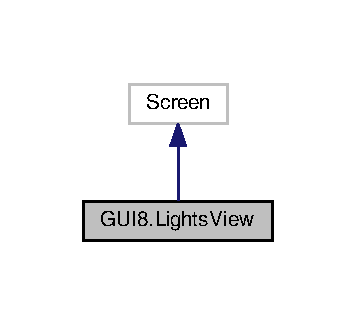
\includegraphics[width=171pt]{classGUI8_1_1LightsView__inherit__graph}
\end{center}
\end{figure}


Collaboration diagram for G\+U\+I8.\+Lights\+View\+:
\nopagebreak
\begin{figure}[H]
\begin{center}
\leavevmode
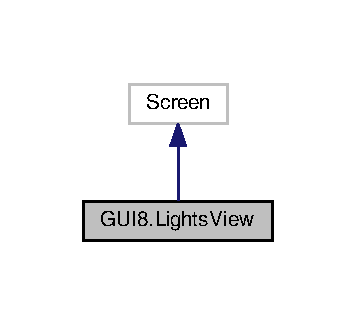
\includegraphics[width=171pt]{classGUI8_1_1LightsView__coll__graph}
\end{center}
\end{figure}
\subsection*{Public Member Functions}
\begin{DoxyCompactItemize}
\item 
def \hyperlink{classGUI8_1_1LightsView_aed889232610f472c1dbf01b8642f97b7}{\+\_\+\+\_\+init\+\_\+\+\_\+} (self, kwargs)
\item 
def \hyperlink{classGUI8_1_1LightsView_aaa45ed32c445502099c5f0c9671d4ca9}{remove\+Light} (self, ip\+\_\+address)
\item 
def \hyperlink{classGUI8_1_1LightsView_a81dd6f4c3010fde8b66a3354a0a58638}{new\+\_\+update} (self, arg1)
\item 
def \hyperlink{classGUI8_1_1LightsView_a447676485186bcb6b0c7974489d708c3}{previous\+\_\+screen} (self, sn, arg2)
\item 
def \hyperlink{classGUI8_1_1LightsView_a4bea440e8f1cb582bb6e5999a6c092bb}{go\+\_\+to\+\_\+view\+\_\+lights} (self, arg1)
\item 
def \hyperlink{classGUI8_1_1LightsView_ada6687e6cce446a0fb04aa126a82ca23}{buildlist} (self)
\item 
def \hyperlink{classGUI8_1_1LightsView_a452671b042632f92e9829044c76fa4c8}{buildlist2} (self, ip)
\item 
def \hyperlink{classGUI8_1_1LightsView_a17953ac1919296fe83ce363045162dfe}{add\+\_\+room} (self)
\item 
def \hyperlink{classGUI8_1_1LightsView_ada549a9f546170b2c5bbe46b61eea033}{lightscallback} (self, instance, value)
\item 
def \hyperlink{classGUI8_1_1LightsView_af234c10fa2c00f715363efc0de45e0c8}{callback} (self, instance, value)
\item 
def \hyperlink{classGUI8_1_1LightsView_adba201635dd08cc14cf993eea2841ae4}{add\+\_\+to\+\_\+room} (self)
\item 
def \hyperlink{classGUI8_1_1LightsView_a3d46689d8b2baa1e006587031c1a177f}{room\+\_\+popup} (self)
\item 
def \hyperlink{classGUI8_1_1LightsView_af6b2eb77701854746eb6617e826bab08}{store} (self, arg1)
\item 
def \hyperlink{classGUI8_1_1LightsView_a248a27eb4031eee351677ab45ea33fad}{update\+\_\+rooms} (self)
\item 
def \hyperlink{classGUI8_1_1LightsView_a8f9ea29dfd8bc7900aca7ec8ecfd6aac}{remove\+\_\+room} (self)
\item 
def \hyperlink{classGUI8_1_1LightsView_a7605161a7f104782ae1babc46e1abc23}{remove\+\_\+light} (self)
\end{DoxyCompactItemize}
\subsection*{Public Attributes}
\begin{DoxyCompactItemize}
\item 
\hyperlink{classGUI8_1_1LightsView_af42477d4f6dce0fdbef3142b50296a60}{textinput}
\end{DoxyCompactItemize}


\subsection{Constructor \& Destructor Documentation}
\index{G\+U\+I8\+::\+Lights\+View@{G\+U\+I8\+::\+Lights\+View}!\+\_\+\+\_\+init\+\_\+\+\_\+@{\+\_\+\+\_\+init\+\_\+\+\_\+}}
\index{\+\_\+\+\_\+init\+\_\+\+\_\+@{\+\_\+\+\_\+init\+\_\+\+\_\+}!G\+U\+I8\+::\+Lights\+View@{G\+U\+I8\+::\+Lights\+View}}
\subsubsection[{\texorpdfstring{\+\_\+\+\_\+init\+\_\+\+\_\+(self, kwargs)}{__init__(self, kwargs)}}]{\setlength{\rightskip}{0pt plus 5cm}def G\+U\+I8.\+Lights\+View.\+\_\+\+\_\+init\+\_\+\+\_\+ (
\begin{DoxyParamCaption}
\item[{}]{self, }
\item[{}]{kwargs}
\end{DoxyParamCaption}
)}\hypertarget{classGUI8_1_1LightsView_aed889232610f472c1dbf01b8642f97b7}{}\label{classGUI8_1_1LightsView_aed889232610f472c1dbf01b8642f97b7}


\subsection{Member Function Documentation}
\index{G\+U\+I8\+::\+Lights\+View@{G\+U\+I8\+::\+Lights\+View}!add\+\_\+room@{add\+\_\+room}}
\index{add\+\_\+room@{add\+\_\+room}!G\+U\+I8\+::\+Lights\+View@{G\+U\+I8\+::\+Lights\+View}}
\subsubsection[{\texorpdfstring{add\+\_\+room(self)}{add_room(self)}}]{\setlength{\rightskip}{0pt plus 5cm}def G\+U\+I8.\+Lights\+View.\+add\+\_\+room (
\begin{DoxyParamCaption}
\item[{}]{self}
\end{DoxyParamCaption}
)}\hypertarget{classGUI8_1_1LightsView_a17953ac1919296fe83ce363045162dfe}{}\label{classGUI8_1_1LightsView_a17953ac1919296fe83ce363045162dfe}
\index{G\+U\+I8\+::\+Lights\+View@{G\+U\+I8\+::\+Lights\+View}!add\+\_\+to\+\_\+room@{add\+\_\+to\+\_\+room}}
\index{add\+\_\+to\+\_\+room@{add\+\_\+to\+\_\+room}!G\+U\+I8\+::\+Lights\+View@{G\+U\+I8\+::\+Lights\+View}}
\subsubsection[{\texorpdfstring{add\+\_\+to\+\_\+room(self)}{add_to_room(self)}}]{\setlength{\rightskip}{0pt plus 5cm}def G\+U\+I8.\+Lights\+View.\+add\+\_\+to\+\_\+room (
\begin{DoxyParamCaption}
\item[{}]{self}
\end{DoxyParamCaption}
)}\hypertarget{classGUI8_1_1LightsView_adba201635dd08cc14cf993eea2841ae4}{}\label{classGUI8_1_1LightsView_adba201635dd08cc14cf993eea2841ae4}
\index{G\+U\+I8\+::\+Lights\+View@{G\+U\+I8\+::\+Lights\+View}!buildlist@{buildlist}}
\index{buildlist@{buildlist}!G\+U\+I8\+::\+Lights\+View@{G\+U\+I8\+::\+Lights\+View}}
\subsubsection[{\texorpdfstring{buildlist(self)}{buildlist(self)}}]{\setlength{\rightskip}{0pt plus 5cm}def G\+U\+I8.\+Lights\+View.\+buildlist (
\begin{DoxyParamCaption}
\item[{}]{self}
\end{DoxyParamCaption}
)}\hypertarget{classGUI8_1_1LightsView_ada6687e6cce446a0fb04aa126a82ca23}{}\label{classGUI8_1_1LightsView_ada6687e6cce446a0fb04aa126a82ca23}
\index{G\+U\+I8\+::\+Lights\+View@{G\+U\+I8\+::\+Lights\+View}!buildlist2@{buildlist2}}
\index{buildlist2@{buildlist2}!G\+U\+I8\+::\+Lights\+View@{G\+U\+I8\+::\+Lights\+View}}
\subsubsection[{\texorpdfstring{buildlist2(self, ip)}{buildlist2(self, ip)}}]{\setlength{\rightskip}{0pt plus 5cm}def G\+U\+I8.\+Lights\+View.\+buildlist2 (
\begin{DoxyParamCaption}
\item[{}]{self, }
\item[{}]{ip}
\end{DoxyParamCaption}
)}\hypertarget{classGUI8_1_1LightsView_a452671b042632f92e9829044c76fa4c8}{}\label{classGUI8_1_1LightsView_a452671b042632f92e9829044c76fa4c8}
\index{G\+U\+I8\+::\+Lights\+View@{G\+U\+I8\+::\+Lights\+View}!callback@{callback}}
\index{callback@{callback}!G\+U\+I8\+::\+Lights\+View@{G\+U\+I8\+::\+Lights\+View}}
\subsubsection[{\texorpdfstring{callback(self, instance, value)}{callback(self, instance, value)}}]{\setlength{\rightskip}{0pt plus 5cm}def G\+U\+I8.\+Lights\+View.\+callback (
\begin{DoxyParamCaption}
\item[{}]{self, }
\item[{}]{instance, }
\item[{}]{value}
\end{DoxyParamCaption}
)}\hypertarget{classGUI8_1_1LightsView_af234c10fa2c00f715363efc0de45e0c8}{}\label{classGUI8_1_1LightsView_af234c10fa2c00f715363efc0de45e0c8}
\index{G\+U\+I8\+::\+Lights\+View@{G\+U\+I8\+::\+Lights\+View}!go\+\_\+to\+\_\+view\+\_\+lights@{go\+\_\+to\+\_\+view\+\_\+lights}}
\index{go\+\_\+to\+\_\+view\+\_\+lights@{go\+\_\+to\+\_\+view\+\_\+lights}!G\+U\+I8\+::\+Lights\+View@{G\+U\+I8\+::\+Lights\+View}}
\subsubsection[{\texorpdfstring{go\+\_\+to\+\_\+view\+\_\+lights(self, arg1)}{go_to_view_lights(self, arg1)}}]{\setlength{\rightskip}{0pt plus 5cm}def G\+U\+I8.\+Lights\+View.\+go\+\_\+to\+\_\+view\+\_\+lights (
\begin{DoxyParamCaption}
\item[{}]{self, }
\item[{}]{arg1}
\end{DoxyParamCaption}
)}\hypertarget{classGUI8_1_1LightsView_a4bea440e8f1cb582bb6e5999a6c092bb}{}\label{classGUI8_1_1LightsView_a4bea440e8f1cb582bb6e5999a6c092bb}
\index{G\+U\+I8\+::\+Lights\+View@{G\+U\+I8\+::\+Lights\+View}!lightscallback@{lightscallback}}
\index{lightscallback@{lightscallback}!G\+U\+I8\+::\+Lights\+View@{G\+U\+I8\+::\+Lights\+View}}
\subsubsection[{\texorpdfstring{lightscallback(self, instance, value)}{lightscallback(self, instance, value)}}]{\setlength{\rightskip}{0pt plus 5cm}def G\+U\+I8.\+Lights\+View.\+lightscallback (
\begin{DoxyParamCaption}
\item[{}]{self, }
\item[{}]{instance, }
\item[{}]{value}
\end{DoxyParamCaption}
)}\hypertarget{classGUI8_1_1LightsView_ada549a9f546170b2c5bbe46b61eea033}{}\label{classGUI8_1_1LightsView_ada549a9f546170b2c5bbe46b61eea033}
\index{G\+U\+I8\+::\+Lights\+View@{G\+U\+I8\+::\+Lights\+View}!new\+\_\+update@{new\+\_\+update}}
\index{new\+\_\+update@{new\+\_\+update}!G\+U\+I8\+::\+Lights\+View@{G\+U\+I8\+::\+Lights\+View}}
\subsubsection[{\texorpdfstring{new\+\_\+update(self, arg1)}{new_update(self, arg1)}}]{\setlength{\rightskip}{0pt plus 5cm}def G\+U\+I8.\+Lights\+View.\+new\+\_\+update (
\begin{DoxyParamCaption}
\item[{}]{self, }
\item[{}]{arg1}
\end{DoxyParamCaption}
)}\hypertarget{classGUI8_1_1LightsView_a81dd6f4c3010fde8b66a3354a0a58638}{}\label{classGUI8_1_1LightsView_a81dd6f4c3010fde8b66a3354a0a58638}
\index{G\+U\+I8\+::\+Lights\+View@{G\+U\+I8\+::\+Lights\+View}!previous\+\_\+screen@{previous\+\_\+screen}}
\index{previous\+\_\+screen@{previous\+\_\+screen}!G\+U\+I8\+::\+Lights\+View@{G\+U\+I8\+::\+Lights\+View}}
\subsubsection[{\texorpdfstring{previous\+\_\+screen(self, sn, arg2)}{previous_screen(self, sn, arg2)}}]{\setlength{\rightskip}{0pt plus 5cm}def G\+U\+I8.\+Lights\+View.\+previous\+\_\+screen (
\begin{DoxyParamCaption}
\item[{}]{self, }
\item[{}]{sn, }
\item[{}]{arg2}
\end{DoxyParamCaption}
)}\hypertarget{classGUI8_1_1LightsView_a447676485186bcb6b0c7974489d708c3}{}\label{classGUI8_1_1LightsView_a447676485186bcb6b0c7974489d708c3}
\index{G\+U\+I8\+::\+Lights\+View@{G\+U\+I8\+::\+Lights\+View}!remove\+\_\+light@{remove\+\_\+light}}
\index{remove\+\_\+light@{remove\+\_\+light}!G\+U\+I8\+::\+Lights\+View@{G\+U\+I8\+::\+Lights\+View}}
\subsubsection[{\texorpdfstring{remove\+\_\+light(self)}{remove_light(self)}}]{\setlength{\rightskip}{0pt plus 5cm}def G\+U\+I8.\+Lights\+View.\+remove\+\_\+light (
\begin{DoxyParamCaption}
\item[{}]{self}
\end{DoxyParamCaption}
)}\hypertarget{classGUI8_1_1LightsView_a7605161a7f104782ae1babc46e1abc23}{}\label{classGUI8_1_1LightsView_a7605161a7f104782ae1babc46e1abc23}
\index{G\+U\+I8\+::\+Lights\+View@{G\+U\+I8\+::\+Lights\+View}!remove\+\_\+room@{remove\+\_\+room}}
\index{remove\+\_\+room@{remove\+\_\+room}!G\+U\+I8\+::\+Lights\+View@{G\+U\+I8\+::\+Lights\+View}}
\subsubsection[{\texorpdfstring{remove\+\_\+room(self)}{remove_room(self)}}]{\setlength{\rightskip}{0pt plus 5cm}def G\+U\+I8.\+Lights\+View.\+remove\+\_\+room (
\begin{DoxyParamCaption}
\item[{}]{self}
\end{DoxyParamCaption}
)}\hypertarget{classGUI8_1_1LightsView_a8f9ea29dfd8bc7900aca7ec8ecfd6aac}{}\label{classGUI8_1_1LightsView_a8f9ea29dfd8bc7900aca7ec8ecfd6aac}
\index{G\+U\+I8\+::\+Lights\+View@{G\+U\+I8\+::\+Lights\+View}!remove\+Light@{remove\+Light}}
\index{remove\+Light@{remove\+Light}!G\+U\+I8\+::\+Lights\+View@{G\+U\+I8\+::\+Lights\+View}}
\subsubsection[{\texorpdfstring{remove\+Light(self, ip\+\_\+address)}{removeLight(self, ip_address)}}]{\setlength{\rightskip}{0pt plus 5cm}def G\+U\+I8.\+Lights\+View.\+remove\+Light (
\begin{DoxyParamCaption}
\item[{}]{self, }
\item[{}]{ip\+\_\+address}
\end{DoxyParamCaption}
)}\hypertarget{classGUI8_1_1LightsView_aaa45ed32c445502099c5f0c9671d4ca9}{}\label{classGUI8_1_1LightsView_aaa45ed32c445502099c5f0c9671d4ca9}
\index{G\+U\+I8\+::\+Lights\+View@{G\+U\+I8\+::\+Lights\+View}!room\+\_\+popup@{room\+\_\+popup}}
\index{room\+\_\+popup@{room\+\_\+popup}!G\+U\+I8\+::\+Lights\+View@{G\+U\+I8\+::\+Lights\+View}}
\subsubsection[{\texorpdfstring{room\+\_\+popup(self)}{room_popup(self)}}]{\setlength{\rightskip}{0pt plus 5cm}def G\+U\+I8.\+Lights\+View.\+room\+\_\+popup (
\begin{DoxyParamCaption}
\item[{}]{self}
\end{DoxyParamCaption}
)}\hypertarget{classGUI8_1_1LightsView_a3d46689d8b2baa1e006587031c1a177f}{}\label{classGUI8_1_1LightsView_a3d46689d8b2baa1e006587031c1a177f}
\index{G\+U\+I8\+::\+Lights\+View@{G\+U\+I8\+::\+Lights\+View}!store@{store}}
\index{store@{store}!G\+U\+I8\+::\+Lights\+View@{G\+U\+I8\+::\+Lights\+View}}
\subsubsection[{\texorpdfstring{store(self, arg1)}{store(self, arg1)}}]{\setlength{\rightskip}{0pt plus 5cm}def G\+U\+I8.\+Lights\+View.\+store (
\begin{DoxyParamCaption}
\item[{}]{self, }
\item[{}]{arg1}
\end{DoxyParamCaption}
)}\hypertarget{classGUI8_1_1LightsView_af6b2eb77701854746eb6617e826bab08}{}\label{classGUI8_1_1LightsView_af6b2eb77701854746eb6617e826bab08}
\index{G\+U\+I8\+::\+Lights\+View@{G\+U\+I8\+::\+Lights\+View}!update\+\_\+rooms@{update\+\_\+rooms}}
\index{update\+\_\+rooms@{update\+\_\+rooms}!G\+U\+I8\+::\+Lights\+View@{G\+U\+I8\+::\+Lights\+View}}
\subsubsection[{\texorpdfstring{update\+\_\+rooms(self)}{update_rooms(self)}}]{\setlength{\rightskip}{0pt plus 5cm}def G\+U\+I8.\+Lights\+View.\+update\+\_\+rooms (
\begin{DoxyParamCaption}
\item[{}]{self}
\end{DoxyParamCaption}
)}\hypertarget{classGUI8_1_1LightsView_a248a27eb4031eee351677ab45ea33fad}{}\label{classGUI8_1_1LightsView_a248a27eb4031eee351677ab45ea33fad}


\subsection{Member Data Documentation}
\index{G\+U\+I8\+::\+Lights\+View@{G\+U\+I8\+::\+Lights\+View}!textinput@{textinput}}
\index{textinput@{textinput}!G\+U\+I8\+::\+Lights\+View@{G\+U\+I8\+::\+Lights\+View}}
\subsubsection[{\texorpdfstring{textinput}{textinput}}]{\setlength{\rightskip}{0pt plus 5cm}G\+U\+I8.\+Lights\+View.\+textinput}\hypertarget{classGUI8_1_1LightsView_af42477d4f6dce0fdbef3142b50296a60}{}\label{classGUI8_1_1LightsView_af42477d4f6dce0fdbef3142b50296a60}


The documentation for this class was generated from the following file\+:\begin{DoxyCompactItemize}
\item 
/home/jac0656/\+Desktop/\+J-\/\+O-\/\+R-\/\+G-\/\+E/\+U\+N\+T-\/\+N\+A\+S\+A/\+G\+U\+I/\hyperlink{GUI8_8py}{G\+U\+I8.\+py}\end{DoxyCompactItemize}

\hypertarget{classGUI8-5pm_1_1LightsView}{}\section{G\+U\+I8-\/5pm.Lights\+View Class Reference}
\label{classGUI8-5pm_1_1LightsView}\index{G\+U\+I8-\/5pm.\+Lights\+View@{G\+U\+I8-\/5pm.\+Lights\+View}}


Inheritance diagram for G\+U\+I8-\/5pm.Lights\+View\+:\nopagebreak
\begin{figure}[H]
\begin{center}
\leavevmode
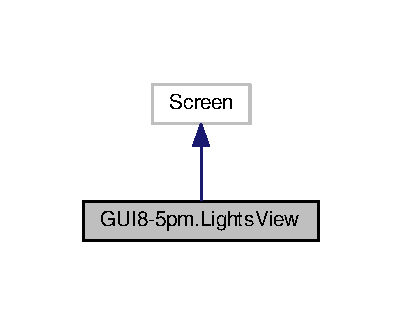
\includegraphics[width=193pt]{classGUI8-5pm_1_1LightsView__inherit__graph}
\end{center}
\end{figure}


Collaboration diagram for G\+U\+I8-\/5pm.Lights\+View\+:\nopagebreak
\begin{figure}[H]
\begin{center}
\leavevmode
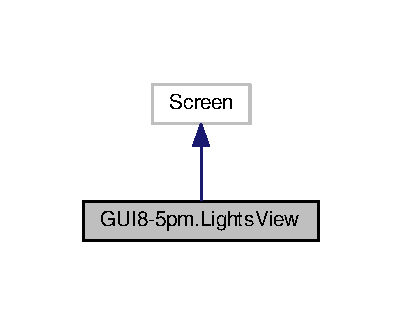
\includegraphics[width=193pt]{classGUI8-5pm_1_1LightsView__coll__graph}
\end{center}
\end{figure}
\subsection*{Public Member Functions}
\begin{DoxyCompactItemize}
\item 
def \hyperlink{classGUI8-5pm_1_1LightsView_ae7d1c4d9cd3566fbd34b713f8d06d1b4}{\+\_\+\+\_\+init\+\_\+\+\_\+} (self, kwargs)
\item 
def \hyperlink{classGUI8-5pm_1_1LightsView_a196136b601af21b35ffa189b52a28c74}{clear\+\_\+lights\+\_\+selection} (self)
\item 
def \hyperlink{classGUI8-5pm_1_1LightsView_a1d8b802d5743ef92638ca488d6c4206b}{remove\+Light} (self, ip\+\_\+addr)
\item 
def \hyperlink{classGUI8-5pm_1_1LightsView_ac67898155faa2ecb2b37af789d4c5da8}{screen\+\_\+update} (self, arg1)
\item 
def \hyperlink{classGUI8-5pm_1_1LightsView_a9e6508b45e002823583b6b3d875bbaa1}{buildlist} (self)
\item 
def \hyperlink{classGUI8-5pm_1_1LightsView_a19236998dfed9a4c815ff47ff3ffdecd}{add\+\_\+room} (self)
\item 
def \hyperlink{classGUI8-5pm_1_1LightsView_aa14040d56fccdb0f91679a01e251ee36}{store\+\_\+state} (self, btn\+\_\+name, \hyperlink{classGUI8-5pm_1_1LightsView_a28bbef7d59d31653b776afd6fcccced6}{btn})
\item 
def \hyperlink{classGUI8-5pm_1_1LightsView_a4a0a8fa02aeb8ddd84fb3ac23350ccf7}{lightscallback} (self, instance, value)
\item 
def \hyperlink{classGUI8-5pm_1_1LightsView_abc262678a2d3186a3f6ee4b404e850bf}{callback} (self, instance, value)
\item 
def \hyperlink{classGUI8-5pm_1_1LightsView_a300f633bf532a37870f3959b3ac0cb3c}{add\+\_\+to\+\_\+room} (self)
\item 
def \hyperlink{classGUI8-5pm_1_1LightsView_a8dfdd625d3c5032e54c3b90266fade52}{room\+\_\+popup} (self)
\item 
def \hyperlink{classGUI8-5pm_1_1LightsView_a1e827d0382e8dc3331a8cb708151d136}{store} (self, arg1)
\item 
def \hyperlink{classGUI8-5pm_1_1LightsView_aefbf28acef5785ce3d4760b783d5f0b8}{update\+\_\+rooms} (self)
\item 
def \hyperlink{classGUI8-5pm_1_1LightsView_a974c9728a6ae53f1da87c96d3c4bde7f}{remove\+\_\+room} (self)
\item 
def \hyperlink{classGUI8-5pm_1_1LightsView_aab2843fb2c86a3a872bc419017d55471}{remove\+\_\+light} (self)
\item 
def \hyperlink{classGUI8-5pm_1_1LightsView_aeaad3431cc072b951752b97515965bbb}{check\+\_\+lights\+\_\+selected} (self)
\item 
def \hyperlink{classGUI8-5pm_1_1LightsView_adfc085a1d001f6a9b6f92238fdc64804}{health\+\_\+check\+\_\+selected} (self)
\end{DoxyCompactItemize}
\subsection*{Public Attributes}
\begin{DoxyCompactItemize}
\item 
\hyperlink{classGUI8-5pm_1_1LightsView_a278c241514a229adb33b8060ef39add5}{layout}
\item 
\hyperlink{classGUI8-5pm_1_1LightsView_a28bbef7d59d31653b776afd6fcccced6}{btn}
\item 
\hyperlink{classGUI8-5pm_1_1LightsView_a4c5fd6f57291537df95d11cf96507abb}{textinput}
\end{DoxyCompactItemize}


\subsection{Constructor \& Destructor Documentation}
\index{G\+U\+I8-\/5pm\+::\+Lights\+View@{G\+U\+I8-\/5pm\+::\+Lights\+View}!\+\_\+\+\_\+init\+\_\+\+\_\+@{\+\_\+\+\_\+init\+\_\+\+\_\+}}
\index{\+\_\+\+\_\+init\+\_\+\+\_\+@{\+\_\+\+\_\+init\+\_\+\+\_\+}!G\+U\+I8-\/5pm\+::\+Lights\+View@{G\+U\+I8-\/5pm\+::\+Lights\+View}}
\subsubsection[{\texorpdfstring{\+\_\+\+\_\+init\+\_\+\+\_\+(self, kwargs)}{__init__(self, kwargs)}}]{\setlength{\rightskip}{0pt plus 5cm}def G\+U\+I8-\/5pm.\+Lights\+View.\+\_\+\+\_\+init\+\_\+\+\_\+ (
\begin{DoxyParamCaption}
\item[{}]{self, }
\item[{}]{kwargs}
\end{DoxyParamCaption}
)}\hypertarget{classGUI8-5pm_1_1LightsView_ae7d1c4d9cd3566fbd34b713f8d06d1b4}{}\label{classGUI8-5pm_1_1LightsView_ae7d1c4d9cd3566fbd34b713f8d06d1b4}


\subsection{Member Function Documentation}
\index{G\+U\+I8-\/5pm\+::\+Lights\+View@{G\+U\+I8-\/5pm\+::\+Lights\+View}!add\+\_\+room@{add\+\_\+room}}
\index{add\+\_\+room@{add\+\_\+room}!G\+U\+I8-\/5pm\+::\+Lights\+View@{G\+U\+I8-\/5pm\+::\+Lights\+View}}
\subsubsection[{\texorpdfstring{add\+\_\+room(self)}{add_room(self)}}]{\setlength{\rightskip}{0pt plus 5cm}def G\+U\+I8-\/5pm.\+Lights\+View.\+add\+\_\+room (
\begin{DoxyParamCaption}
\item[{}]{self}
\end{DoxyParamCaption}
)}\hypertarget{classGUI8-5pm_1_1LightsView_a19236998dfed9a4c815ff47ff3ffdecd}{}\label{classGUI8-5pm_1_1LightsView_a19236998dfed9a4c815ff47ff3ffdecd}
\index{G\+U\+I8-\/5pm\+::\+Lights\+View@{G\+U\+I8-\/5pm\+::\+Lights\+View}!add\+\_\+to\+\_\+room@{add\+\_\+to\+\_\+room}}
\index{add\+\_\+to\+\_\+room@{add\+\_\+to\+\_\+room}!G\+U\+I8-\/5pm\+::\+Lights\+View@{G\+U\+I8-\/5pm\+::\+Lights\+View}}
\subsubsection[{\texorpdfstring{add\+\_\+to\+\_\+room(self)}{add_to_room(self)}}]{\setlength{\rightskip}{0pt plus 5cm}def G\+U\+I8-\/5pm.\+Lights\+View.\+add\+\_\+to\+\_\+room (
\begin{DoxyParamCaption}
\item[{}]{self}
\end{DoxyParamCaption}
)}\hypertarget{classGUI8-5pm_1_1LightsView_a300f633bf532a37870f3959b3ac0cb3c}{}\label{classGUI8-5pm_1_1LightsView_a300f633bf532a37870f3959b3ac0cb3c}
\index{G\+U\+I8-\/5pm\+::\+Lights\+View@{G\+U\+I8-\/5pm\+::\+Lights\+View}!buildlist@{buildlist}}
\index{buildlist@{buildlist}!G\+U\+I8-\/5pm\+::\+Lights\+View@{G\+U\+I8-\/5pm\+::\+Lights\+View}}
\subsubsection[{\texorpdfstring{buildlist(self)}{buildlist(self)}}]{\setlength{\rightskip}{0pt plus 5cm}def G\+U\+I8-\/5pm.\+Lights\+View.\+buildlist (
\begin{DoxyParamCaption}
\item[{}]{self}
\end{DoxyParamCaption}
)}\hypertarget{classGUI8-5pm_1_1LightsView_a9e6508b45e002823583b6b3d875bbaa1}{}\label{classGUI8-5pm_1_1LightsView_a9e6508b45e002823583b6b3d875bbaa1}
\index{G\+U\+I8-\/5pm\+::\+Lights\+View@{G\+U\+I8-\/5pm\+::\+Lights\+View}!callback@{callback}}
\index{callback@{callback}!G\+U\+I8-\/5pm\+::\+Lights\+View@{G\+U\+I8-\/5pm\+::\+Lights\+View}}
\subsubsection[{\texorpdfstring{callback(self, instance, value)}{callback(self, instance, value)}}]{\setlength{\rightskip}{0pt plus 5cm}def G\+U\+I8-\/5pm.\+Lights\+View.\+callback (
\begin{DoxyParamCaption}
\item[{}]{self, }
\item[{}]{instance, }
\item[{}]{value}
\end{DoxyParamCaption}
)}\hypertarget{classGUI8-5pm_1_1LightsView_abc262678a2d3186a3f6ee4b404e850bf}{}\label{classGUI8-5pm_1_1LightsView_abc262678a2d3186a3f6ee4b404e850bf}
\index{G\+U\+I8-\/5pm\+::\+Lights\+View@{G\+U\+I8-\/5pm\+::\+Lights\+View}!check\+\_\+lights\+\_\+selected@{check\+\_\+lights\+\_\+selected}}
\index{check\+\_\+lights\+\_\+selected@{check\+\_\+lights\+\_\+selected}!G\+U\+I8-\/5pm\+::\+Lights\+View@{G\+U\+I8-\/5pm\+::\+Lights\+View}}
\subsubsection[{\texorpdfstring{check\+\_\+lights\+\_\+selected(self)}{check_lights_selected(self)}}]{\setlength{\rightskip}{0pt plus 5cm}def G\+U\+I8-\/5pm.\+Lights\+View.\+check\+\_\+lights\+\_\+selected (
\begin{DoxyParamCaption}
\item[{}]{self}
\end{DoxyParamCaption}
)}\hypertarget{classGUI8-5pm_1_1LightsView_aeaad3431cc072b951752b97515965bbb}{}\label{classGUI8-5pm_1_1LightsView_aeaad3431cc072b951752b97515965bbb}
\index{G\+U\+I8-\/5pm\+::\+Lights\+View@{G\+U\+I8-\/5pm\+::\+Lights\+View}!clear\+\_\+lights\+\_\+selection@{clear\+\_\+lights\+\_\+selection}}
\index{clear\+\_\+lights\+\_\+selection@{clear\+\_\+lights\+\_\+selection}!G\+U\+I8-\/5pm\+::\+Lights\+View@{G\+U\+I8-\/5pm\+::\+Lights\+View}}
\subsubsection[{\texorpdfstring{clear\+\_\+lights\+\_\+selection(self)}{clear_lights_selection(self)}}]{\setlength{\rightskip}{0pt plus 5cm}def G\+U\+I8-\/5pm.\+Lights\+View.\+clear\+\_\+lights\+\_\+selection (
\begin{DoxyParamCaption}
\item[{}]{self}
\end{DoxyParamCaption}
)}\hypertarget{classGUI8-5pm_1_1LightsView_a196136b601af21b35ffa189b52a28c74}{}\label{classGUI8-5pm_1_1LightsView_a196136b601af21b35ffa189b52a28c74}
\index{G\+U\+I8-\/5pm\+::\+Lights\+View@{G\+U\+I8-\/5pm\+::\+Lights\+View}!health\+\_\+check\+\_\+selected@{health\+\_\+check\+\_\+selected}}
\index{health\+\_\+check\+\_\+selected@{health\+\_\+check\+\_\+selected}!G\+U\+I8-\/5pm\+::\+Lights\+View@{G\+U\+I8-\/5pm\+::\+Lights\+View}}
\subsubsection[{\texorpdfstring{health\+\_\+check\+\_\+selected(self)}{health_check_selected(self)}}]{\setlength{\rightskip}{0pt plus 5cm}def G\+U\+I8-\/5pm.\+Lights\+View.\+health\+\_\+check\+\_\+selected (
\begin{DoxyParamCaption}
\item[{}]{self}
\end{DoxyParamCaption}
)}\hypertarget{classGUI8-5pm_1_1LightsView_adfc085a1d001f6a9b6f92238fdc64804}{}\label{classGUI8-5pm_1_1LightsView_adfc085a1d001f6a9b6f92238fdc64804}
\index{G\+U\+I8-\/5pm\+::\+Lights\+View@{G\+U\+I8-\/5pm\+::\+Lights\+View}!lightscallback@{lightscallback}}
\index{lightscallback@{lightscallback}!G\+U\+I8-\/5pm\+::\+Lights\+View@{G\+U\+I8-\/5pm\+::\+Lights\+View}}
\subsubsection[{\texorpdfstring{lightscallback(self, instance, value)}{lightscallback(self, instance, value)}}]{\setlength{\rightskip}{0pt plus 5cm}def G\+U\+I8-\/5pm.\+Lights\+View.\+lightscallback (
\begin{DoxyParamCaption}
\item[{}]{self, }
\item[{}]{instance, }
\item[{}]{value}
\end{DoxyParamCaption}
)}\hypertarget{classGUI8-5pm_1_1LightsView_a4a0a8fa02aeb8ddd84fb3ac23350ccf7}{}\label{classGUI8-5pm_1_1LightsView_a4a0a8fa02aeb8ddd84fb3ac23350ccf7}
\index{G\+U\+I8-\/5pm\+::\+Lights\+View@{G\+U\+I8-\/5pm\+::\+Lights\+View}!remove\+\_\+light@{remove\+\_\+light}}
\index{remove\+\_\+light@{remove\+\_\+light}!G\+U\+I8-\/5pm\+::\+Lights\+View@{G\+U\+I8-\/5pm\+::\+Lights\+View}}
\subsubsection[{\texorpdfstring{remove\+\_\+light(self)}{remove_light(self)}}]{\setlength{\rightskip}{0pt plus 5cm}def G\+U\+I8-\/5pm.\+Lights\+View.\+remove\+\_\+light (
\begin{DoxyParamCaption}
\item[{}]{self}
\end{DoxyParamCaption}
)}\hypertarget{classGUI8-5pm_1_1LightsView_aab2843fb2c86a3a872bc419017d55471}{}\label{classGUI8-5pm_1_1LightsView_aab2843fb2c86a3a872bc419017d55471}
\index{G\+U\+I8-\/5pm\+::\+Lights\+View@{G\+U\+I8-\/5pm\+::\+Lights\+View}!remove\+\_\+room@{remove\+\_\+room}}
\index{remove\+\_\+room@{remove\+\_\+room}!G\+U\+I8-\/5pm\+::\+Lights\+View@{G\+U\+I8-\/5pm\+::\+Lights\+View}}
\subsubsection[{\texorpdfstring{remove\+\_\+room(self)}{remove_room(self)}}]{\setlength{\rightskip}{0pt plus 5cm}def G\+U\+I8-\/5pm.\+Lights\+View.\+remove\+\_\+room (
\begin{DoxyParamCaption}
\item[{}]{self}
\end{DoxyParamCaption}
)}\hypertarget{classGUI8-5pm_1_1LightsView_a974c9728a6ae53f1da87c96d3c4bde7f}{}\label{classGUI8-5pm_1_1LightsView_a974c9728a6ae53f1da87c96d3c4bde7f}
\index{G\+U\+I8-\/5pm\+::\+Lights\+View@{G\+U\+I8-\/5pm\+::\+Lights\+View}!remove\+Light@{remove\+Light}}
\index{remove\+Light@{remove\+Light}!G\+U\+I8-\/5pm\+::\+Lights\+View@{G\+U\+I8-\/5pm\+::\+Lights\+View}}
\subsubsection[{\texorpdfstring{remove\+Light(self, ip\+\_\+addr)}{removeLight(self, ip_addr)}}]{\setlength{\rightskip}{0pt plus 5cm}def G\+U\+I8-\/5pm.\+Lights\+View.\+remove\+Light (
\begin{DoxyParamCaption}
\item[{}]{self, }
\item[{}]{ip\+\_\+addr}
\end{DoxyParamCaption}
)}\hypertarget{classGUI8-5pm_1_1LightsView_a1d8b802d5743ef92638ca488d6c4206b}{}\label{classGUI8-5pm_1_1LightsView_a1d8b802d5743ef92638ca488d6c4206b}
\index{G\+U\+I8-\/5pm\+::\+Lights\+View@{G\+U\+I8-\/5pm\+::\+Lights\+View}!room\+\_\+popup@{room\+\_\+popup}}
\index{room\+\_\+popup@{room\+\_\+popup}!G\+U\+I8-\/5pm\+::\+Lights\+View@{G\+U\+I8-\/5pm\+::\+Lights\+View}}
\subsubsection[{\texorpdfstring{room\+\_\+popup(self)}{room_popup(self)}}]{\setlength{\rightskip}{0pt plus 5cm}def G\+U\+I8-\/5pm.\+Lights\+View.\+room\+\_\+popup (
\begin{DoxyParamCaption}
\item[{}]{self}
\end{DoxyParamCaption}
)}\hypertarget{classGUI8-5pm_1_1LightsView_a8dfdd625d3c5032e54c3b90266fade52}{}\label{classGUI8-5pm_1_1LightsView_a8dfdd625d3c5032e54c3b90266fade52}
\index{G\+U\+I8-\/5pm\+::\+Lights\+View@{G\+U\+I8-\/5pm\+::\+Lights\+View}!screen\+\_\+update@{screen\+\_\+update}}
\index{screen\+\_\+update@{screen\+\_\+update}!G\+U\+I8-\/5pm\+::\+Lights\+View@{G\+U\+I8-\/5pm\+::\+Lights\+View}}
\subsubsection[{\texorpdfstring{screen\+\_\+update(self, arg1)}{screen_update(self, arg1)}}]{\setlength{\rightskip}{0pt plus 5cm}def G\+U\+I8-\/5pm.\+Lights\+View.\+screen\+\_\+update (
\begin{DoxyParamCaption}
\item[{}]{self, }
\item[{}]{arg1}
\end{DoxyParamCaption}
)}\hypertarget{classGUI8-5pm_1_1LightsView_ac67898155faa2ecb2b37af789d4c5da8}{}\label{classGUI8-5pm_1_1LightsView_ac67898155faa2ecb2b37af789d4c5da8}
\index{G\+U\+I8-\/5pm\+::\+Lights\+View@{G\+U\+I8-\/5pm\+::\+Lights\+View}!store@{store}}
\index{store@{store}!G\+U\+I8-\/5pm\+::\+Lights\+View@{G\+U\+I8-\/5pm\+::\+Lights\+View}}
\subsubsection[{\texorpdfstring{store(self, arg1)}{store(self, arg1)}}]{\setlength{\rightskip}{0pt plus 5cm}def G\+U\+I8-\/5pm.\+Lights\+View.\+store (
\begin{DoxyParamCaption}
\item[{}]{self, }
\item[{}]{arg1}
\end{DoxyParamCaption}
)}\hypertarget{classGUI8-5pm_1_1LightsView_a1e827d0382e8dc3331a8cb708151d136}{}\label{classGUI8-5pm_1_1LightsView_a1e827d0382e8dc3331a8cb708151d136}
\index{G\+U\+I8-\/5pm\+::\+Lights\+View@{G\+U\+I8-\/5pm\+::\+Lights\+View}!store\+\_\+state@{store\+\_\+state}}
\index{store\+\_\+state@{store\+\_\+state}!G\+U\+I8-\/5pm\+::\+Lights\+View@{G\+U\+I8-\/5pm\+::\+Lights\+View}}
\subsubsection[{\texorpdfstring{store\+\_\+state(self, btn\+\_\+name, btn)}{store_state(self, btn_name, btn)}}]{\setlength{\rightskip}{0pt plus 5cm}def G\+U\+I8-\/5pm.\+Lights\+View.\+store\+\_\+state (
\begin{DoxyParamCaption}
\item[{}]{self, }
\item[{}]{btn\+\_\+name, }
\item[{}]{btn}
\end{DoxyParamCaption}
)}\hypertarget{classGUI8-5pm_1_1LightsView_aa14040d56fccdb0f91679a01e251ee36}{}\label{classGUI8-5pm_1_1LightsView_aa14040d56fccdb0f91679a01e251ee36}
\index{G\+U\+I8-\/5pm\+::\+Lights\+View@{G\+U\+I8-\/5pm\+::\+Lights\+View}!update\+\_\+rooms@{update\+\_\+rooms}}
\index{update\+\_\+rooms@{update\+\_\+rooms}!G\+U\+I8-\/5pm\+::\+Lights\+View@{G\+U\+I8-\/5pm\+::\+Lights\+View}}
\subsubsection[{\texorpdfstring{update\+\_\+rooms(self)}{update_rooms(self)}}]{\setlength{\rightskip}{0pt plus 5cm}def G\+U\+I8-\/5pm.\+Lights\+View.\+update\+\_\+rooms (
\begin{DoxyParamCaption}
\item[{}]{self}
\end{DoxyParamCaption}
)}\hypertarget{classGUI8-5pm_1_1LightsView_aefbf28acef5785ce3d4760b783d5f0b8}{}\label{classGUI8-5pm_1_1LightsView_aefbf28acef5785ce3d4760b783d5f0b8}


\subsection{Member Data Documentation}
\index{G\+U\+I8-\/5pm\+::\+Lights\+View@{G\+U\+I8-\/5pm\+::\+Lights\+View}!btn@{btn}}
\index{btn@{btn}!G\+U\+I8-\/5pm\+::\+Lights\+View@{G\+U\+I8-\/5pm\+::\+Lights\+View}}
\subsubsection[{\texorpdfstring{btn}{btn}}]{\setlength{\rightskip}{0pt plus 5cm}G\+U\+I8-\/5pm.\+Lights\+View.\+btn}\hypertarget{classGUI8-5pm_1_1LightsView_a28bbef7d59d31653b776afd6fcccced6}{}\label{classGUI8-5pm_1_1LightsView_a28bbef7d59d31653b776afd6fcccced6}
\index{G\+U\+I8-\/5pm\+::\+Lights\+View@{G\+U\+I8-\/5pm\+::\+Lights\+View}!layout@{layout}}
\index{layout@{layout}!G\+U\+I8-\/5pm\+::\+Lights\+View@{G\+U\+I8-\/5pm\+::\+Lights\+View}}
\subsubsection[{\texorpdfstring{layout}{layout}}]{\setlength{\rightskip}{0pt plus 5cm}G\+U\+I8-\/5pm.\+Lights\+View.\+layout}\hypertarget{classGUI8-5pm_1_1LightsView_a278c241514a229adb33b8060ef39add5}{}\label{classGUI8-5pm_1_1LightsView_a278c241514a229adb33b8060ef39add5}
\index{G\+U\+I8-\/5pm\+::\+Lights\+View@{G\+U\+I8-\/5pm\+::\+Lights\+View}!textinput@{textinput}}
\index{textinput@{textinput}!G\+U\+I8-\/5pm\+::\+Lights\+View@{G\+U\+I8-\/5pm\+::\+Lights\+View}}
\subsubsection[{\texorpdfstring{textinput}{textinput}}]{\setlength{\rightskip}{0pt plus 5cm}G\+U\+I8-\/5pm.\+Lights\+View.\+textinput}\hypertarget{classGUI8-5pm_1_1LightsView_a4c5fd6f57291537df95d11cf96507abb}{}\label{classGUI8-5pm_1_1LightsView_a4c5fd6f57291537df95d11cf96507abb}


The documentation for this class was generated from the following file\+:\begin{DoxyCompactItemize}
\item 
/home/jac0656/\+Desktop/\+J-\/\+O-\/\+R-\/\+G-\/\+E/\+U\+N\+T-\/\+N\+A\+S\+A/\hyperlink{GUI8-5pm_8py}{G\+U\+I8-\/5pm.\+py}\end{DoxyCompactItemize}

\hypertarget{classnewGUI_1_1LightsView}{}\section{new\+G\+U\+I.\+Lights\+View Class Reference}
\label{classnewGUI_1_1LightsView}\index{new\+G\+U\+I.\+Lights\+View@{new\+G\+U\+I.\+Lights\+View}}


Inheritance diagram for new\+G\+U\+I.\+Lights\+View\+:
\nopagebreak
\begin{figure}[H]
\begin{center}
\leavevmode
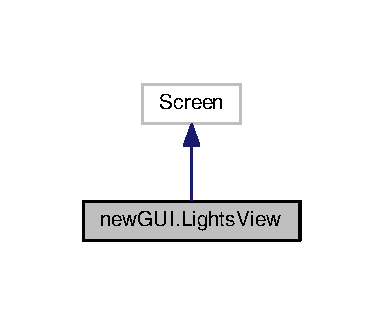
\includegraphics[width=184pt]{classnewGUI_1_1LightsView__inherit__graph}
\end{center}
\end{figure}


Collaboration diagram for new\+G\+U\+I.\+Lights\+View\+:
\nopagebreak
\begin{figure}[H]
\begin{center}
\leavevmode
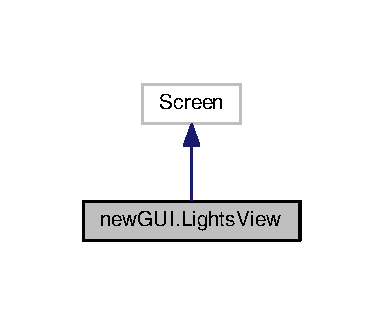
\includegraphics[width=184pt]{classnewGUI_1_1LightsView__coll__graph}
\end{center}
\end{figure}
\subsection*{Public Member Functions}
\begin{DoxyCompactItemize}
\item 
def \hyperlink{classnewGUI_1_1LightsView_a590a6030e2ddea8da13d73996488b22e}{\+\_\+\+\_\+init\+\_\+\+\_\+} (self, kwargs)
\item 
def \hyperlink{classnewGUI_1_1LightsView_a231483bb8ed2747a96bc6baed824ec15}{remove\+Light} (self, ip\+\_\+address)
\item 
def \hyperlink{classnewGUI_1_1LightsView_ab75b0dda22fd1237684f0ae7745af08f}{new\+\_\+update} (self, arg1)
\item 
def \hyperlink{classnewGUI_1_1LightsView_a462ca851ac6c1980ea719d1901975b85}{previous\+\_\+screen} (self, sn, arg2)
\item 
def \hyperlink{classnewGUI_1_1LightsView_a6b910b71b740b4000448b9a97e8acb06}{go\+\_\+to\+\_\+view\+\_\+lights} (self, arg1)
\item 
def \hyperlink{classnewGUI_1_1LightsView_accb8167477c948965c95d97a31b80491}{buildlist} (self)
\item 
def \hyperlink{classnewGUI_1_1LightsView_a220bbeabf0b68b672f1e063177599863}{buildlist2} (self, ip)
\item 
def \hyperlink{classnewGUI_1_1LightsView_a76778ba2371697002697761ba2739ee8}{add\+\_\+room} (self)
\item 
def \hyperlink{classnewGUI_1_1LightsView_ac54610df21a705ca392d60cca664e02c}{lightscallback} (self, instance, value)
\item 
def \hyperlink{classnewGUI_1_1LightsView_af8827a7ac6c87c23a02ea489e106ca59}{callback} (self, instance, value)
\item 
def \hyperlink{classnewGUI_1_1LightsView_a54dfc210a4c1b43d9695be700eac59b5}{add\+\_\+to\+\_\+room} (self)
\item 
def \hyperlink{classnewGUI_1_1LightsView_adcb4018224aad7c127afc8f8eafed2de}{room\+\_\+popup} (self)
\item 
def \hyperlink{classnewGUI_1_1LightsView_a6dc9e9bbd7015b938fbda7553530a33b}{store} (self, arg1)
\item 
def \hyperlink{classnewGUI_1_1LightsView_a3fd62c3ea4a8583bdf29d3ac2175c773}{update\+\_\+rooms} (self)
\item 
def \hyperlink{classnewGUI_1_1LightsView_ae90470e51371adbf0b2c9a6029a457d7}{remove\+\_\+room} (self)
\item 
def \hyperlink{classnewGUI_1_1LightsView_a6fc29fe88f9e381f748c0fe168abfb85}{remove\+\_\+light} (self)
\end{DoxyCompactItemize}
\subsection*{Public Attributes}
\begin{DoxyCompactItemize}
\item 
\hyperlink{classnewGUI_1_1LightsView_a842cc321c570d7f287031574efb44c6c}{textinput}
\end{DoxyCompactItemize}


\subsection{Constructor \& Destructor Documentation}
\index{new\+G\+U\+I\+::\+Lights\+View@{new\+G\+U\+I\+::\+Lights\+View}!\+\_\+\+\_\+init\+\_\+\+\_\+@{\+\_\+\+\_\+init\+\_\+\+\_\+}}
\index{\+\_\+\+\_\+init\+\_\+\+\_\+@{\+\_\+\+\_\+init\+\_\+\+\_\+}!new\+G\+U\+I\+::\+Lights\+View@{new\+G\+U\+I\+::\+Lights\+View}}
\subsubsection[{\texorpdfstring{\+\_\+\+\_\+init\+\_\+\+\_\+(self, kwargs)}{__init__(self, kwargs)}}]{\setlength{\rightskip}{0pt plus 5cm}def new\+G\+U\+I.\+Lights\+View.\+\_\+\+\_\+init\+\_\+\+\_\+ (
\begin{DoxyParamCaption}
\item[{}]{self, }
\item[{}]{kwargs}
\end{DoxyParamCaption}
)}\hypertarget{classnewGUI_1_1LightsView_a590a6030e2ddea8da13d73996488b22e}{}\label{classnewGUI_1_1LightsView_a590a6030e2ddea8da13d73996488b22e}


\subsection{Member Function Documentation}
\index{new\+G\+U\+I\+::\+Lights\+View@{new\+G\+U\+I\+::\+Lights\+View}!add\+\_\+room@{add\+\_\+room}}
\index{add\+\_\+room@{add\+\_\+room}!new\+G\+U\+I\+::\+Lights\+View@{new\+G\+U\+I\+::\+Lights\+View}}
\subsubsection[{\texorpdfstring{add\+\_\+room(self)}{add_room(self)}}]{\setlength{\rightskip}{0pt plus 5cm}def new\+G\+U\+I.\+Lights\+View.\+add\+\_\+room (
\begin{DoxyParamCaption}
\item[{}]{self}
\end{DoxyParamCaption}
)}\hypertarget{classnewGUI_1_1LightsView_a76778ba2371697002697761ba2739ee8}{}\label{classnewGUI_1_1LightsView_a76778ba2371697002697761ba2739ee8}
\index{new\+G\+U\+I\+::\+Lights\+View@{new\+G\+U\+I\+::\+Lights\+View}!add\+\_\+to\+\_\+room@{add\+\_\+to\+\_\+room}}
\index{add\+\_\+to\+\_\+room@{add\+\_\+to\+\_\+room}!new\+G\+U\+I\+::\+Lights\+View@{new\+G\+U\+I\+::\+Lights\+View}}
\subsubsection[{\texorpdfstring{add\+\_\+to\+\_\+room(self)}{add_to_room(self)}}]{\setlength{\rightskip}{0pt plus 5cm}def new\+G\+U\+I.\+Lights\+View.\+add\+\_\+to\+\_\+room (
\begin{DoxyParamCaption}
\item[{}]{self}
\end{DoxyParamCaption}
)}\hypertarget{classnewGUI_1_1LightsView_a54dfc210a4c1b43d9695be700eac59b5}{}\label{classnewGUI_1_1LightsView_a54dfc210a4c1b43d9695be700eac59b5}
\index{new\+G\+U\+I\+::\+Lights\+View@{new\+G\+U\+I\+::\+Lights\+View}!buildlist@{buildlist}}
\index{buildlist@{buildlist}!new\+G\+U\+I\+::\+Lights\+View@{new\+G\+U\+I\+::\+Lights\+View}}
\subsubsection[{\texorpdfstring{buildlist(self)}{buildlist(self)}}]{\setlength{\rightskip}{0pt plus 5cm}def new\+G\+U\+I.\+Lights\+View.\+buildlist (
\begin{DoxyParamCaption}
\item[{}]{self}
\end{DoxyParamCaption}
)}\hypertarget{classnewGUI_1_1LightsView_accb8167477c948965c95d97a31b80491}{}\label{classnewGUI_1_1LightsView_accb8167477c948965c95d97a31b80491}
\index{new\+G\+U\+I\+::\+Lights\+View@{new\+G\+U\+I\+::\+Lights\+View}!buildlist2@{buildlist2}}
\index{buildlist2@{buildlist2}!new\+G\+U\+I\+::\+Lights\+View@{new\+G\+U\+I\+::\+Lights\+View}}
\subsubsection[{\texorpdfstring{buildlist2(self, ip)}{buildlist2(self, ip)}}]{\setlength{\rightskip}{0pt plus 5cm}def new\+G\+U\+I.\+Lights\+View.\+buildlist2 (
\begin{DoxyParamCaption}
\item[{}]{self, }
\item[{}]{ip}
\end{DoxyParamCaption}
)}\hypertarget{classnewGUI_1_1LightsView_a220bbeabf0b68b672f1e063177599863}{}\label{classnewGUI_1_1LightsView_a220bbeabf0b68b672f1e063177599863}
\index{new\+G\+U\+I\+::\+Lights\+View@{new\+G\+U\+I\+::\+Lights\+View}!callback@{callback}}
\index{callback@{callback}!new\+G\+U\+I\+::\+Lights\+View@{new\+G\+U\+I\+::\+Lights\+View}}
\subsubsection[{\texorpdfstring{callback(self, instance, value)}{callback(self, instance, value)}}]{\setlength{\rightskip}{0pt plus 5cm}def new\+G\+U\+I.\+Lights\+View.\+callback (
\begin{DoxyParamCaption}
\item[{}]{self, }
\item[{}]{instance, }
\item[{}]{value}
\end{DoxyParamCaption}
)}\hypertarget{classnewGUI_1_1LightsView_af8827a7ac6c87c23a02ea489e106ca59}{}\label{classnewGUI_1_1LightsView_af8827a7ac6c87c23a02ea489e106ca59}
\index{new\+G\+U\+I\+::\+Lights\+View@{new\+G\+U\+I\+::\+Lights\+View}!go\+\_\+to\+\_\+view\+\_\+lights@{go\+\_\+to\+\_\+view\+\_\+lights}}
\index{go\+\_\+to\+\_\+view\+\_\+lights@{go\+\_\+to\+\_\+view\+\_\+lights}!new\+G\+U\+I\+::\+Lights\+View@{new\+G\+U\+I\+::\+Lights\+View}}
\subsubsection[{\texorpdfstring{go\+\_\+to\+\_\+view\+\_\+lights(self, arg1)}{go_to_view_lights(self, arg1)}}]{\setlength{\rightskip}{0pt plus 5cm}def new\+G\+U\+I.\+Lights\+View.\+go\+\_\+to\+\_\+view\+\_\+lights (
\begin{DoxyParamCaption}
\item[{}]{self, }
\item[{}]{arg1}
\end{DoxyParamCaption}
)}\hypertarget{classnewGUI_1_1LightsView_a6b910b71b740b4000448b9a97e8acb06}{}\label{classnewGUI_1_1LightsView_a6b910b71b740b4000448b9a97e8acb06}
\index{new\+G\+U\+I\+::\+Lights\+View@{new\+G\+U\+I\+::\+Lights\+View}!lightscallback@{lightscallback}}
\index{lightscallback@{lightscallback}!new\+G\+U\+I\+::\+Lights\+View@{new\+G\+U\+I\+::\+Lights\+View}}
\subsubsection[{\texorpdfstring{lightscallback(self, instance, value)}{lightscallback(self, instance, value)}}]{\setlength{\rightskip}{0pt plus 5cm}def new\+G\+U\+I.\+Lights\+View.\+lightscallback (
\begin{DoxyParamCaption}
\item[{}]{self, }
\item[{}]{instance, }
\item[{}]{value}
\end{DoxyParamCaption}
)}\hypertarget{classnewGUI_1_1LightsView_ac54610df21a705ca392d60cca664e02c}{}\label{classnewGUI_1_1LightsView_ac54610df21a705ca392d60cca664e02c}
\index{new\+G\+U\+I\+::\+Lights\+View@{new\+G\+U\+I\+::\+Lights\+View}!new\+\_\+update@{new\+\_\+update}}
\index{new\+\_\+update@{new\+\_\+update}!new\+G\+U\+I\+::\+Lights\+View@{new\+G\+U\+I\+::\+Lights\+View}}
\subsubsection[{\texorpdfstring{new\+\_\+update(self, arg1)}{new_update(self, arg1)}}]{\setlength{\rightskip}{0pt plus 5cm}def new\+G\+U\+I.\+Lights\+View.\+new\+\_\+update (
\begin{DoxyParamCaption}
\item[{}]{self, }
\item[{}]{arg1}
\end{DoxyParamCaption}
)}\hypertarget{classnewGUI_1_1LightsView_ab75b0dda22fd1237684f0ae7745af08f}{}\label{classnewGUI_1_1LightsView_ab75b0dda22fd1237684f0ae7745af08f}
\index{new\+G\+U\+I\+::\+Lights\+View@{new\+G\+U\+I\+::\+Lights\+View}!previous\+\_\+screen@{previous\+\_\+screen}}
\index{previous\+\_\+screen@{previous\+\_\+screen}!new\+G\+U\+I\+::\+Lights\+View@{new\+G\+U\+I\+::\+Lights\+View}}
\subsubsection[{\texorpdfstring{previous\+\_\+screen(self, sn, arg2)}{previous_screen(self, sn, arg2)}}]{\setlength{\rightskip}{0pt plus 5cm}def new\+G\+U\+I.\+Lights\+View.\+previous\+\_\+screen (
\begin{DoxyParamCaption}
\item[{}]{self, }
\item[{}]{sn, }
\item[{}]{arg2}
\end{DoxyParamCaption}
)}\hypertarget{classnewGUI_1_1LightsView_a462ca851ac6c1980ea719d1901975b85}{}\label{classnewGUI_1_1LightsView_a462ca851ac6c1980ea719d1901975b85}
\index{new\+G\+U\+I\+::\+Lights\+View@{new\+G\+U\+I\+::\+Lights\+View}!remove\+\_\+light@{remove\+\_\+light}}
\index{remove\+\_\+light@{remove\+\_\+light}!new\+G\+U\+I\+::\+Lights\+View@{new\+G\+U\+I\+::\+Lights\+View}}
\subsubsection[{\texorpdfstring{remove\+\_\+light(self)}{remove_light(self)}}]{\setlength{\rightskip}{0pt plus 5cm}def new\+G\+U\+I.\+Lights\+View.\+remove\+\_\+light (
\begin{DoxyParamCaption}
\item[{}]{self}
\end{DoxyParamCaption}
)}\hypertarget{classnewGUI_1_1LightsView_a6fc29fe88f9e381f748c0fe168abfb85}{}\label{classnewGUI_1_1LightsView_a6fc29fe88f9e381f748c0fe168abfb85}
\index{new\+G\+U\+I\+::\+Lights\+View@{new\+G\+U\+I\+::\+Lights\+View}!remove\+\_\+room@{remove\+\_\+room}}
\index{remove\+\_\+room@{remove\+\_\+room}!new\+G\+U\+I\+::\+Lights\+View@{new\+G\+U\+I\+::\+Lights\+View}}
\subsubsection[{\texorpdfstring{remove\+\_\+room(self)}{remove_room(self)}}]{\setlength{\rightskip}{0pt plus 5cm}def new\+G\+U\+I.\+Lights\+View.\+remove\+\_\+room (
\begin{DoxyParamCaption}
\item[{}]{self}
\end{DoxyParamCaption}
)}\hypertarget{classnewGUI_1_1LightsView_ae90470e51371adbf0b2c9a6029a457d7}{}\label{classnewGUI_1_1LightsView_ae90470e51371adbf0b2c9a6029a457d7}
\index{new\+G\+U\+I\+::\+Lights\+View@{new\+G\+U\+I\+::\+Lights\+View}!remove\+Light@{remove\+Light}}
\index{remove\+Light@{remove\+Light}!new\+G\+U\+I\+::\+Lights\+View@{new\+G\+U\+I\+::\+Lights\+View}}
\subsubsection[{\texorpdfstring{remove\+Light(self, ip\+\_\+address)}{removeLight(self, ip_address)}}]{\setlength{\rightskip}{0pt plus 5cm}def new\+G\+U\+I.\+Lights\+View.\+remove\+Light (
\begin{DoxyParamCaption}
\item[{}]{self, }
\item[{}]{ip\+\_\+address}
\end{DoxyParamCaption}
)}\hypertarget{classnewGUI_1_1LightsView_a231483bb8ed2747a96bc6baed824ec15}{}\label{classnewGUI_1_1LightsView_a231483bb8ed2747a96bc6baed824ec15}
\index{new\+G\+U\+I\+::\+Lights\+View@{new\+G\+U\+I\+::\+Lights\+View}!room\+\_\+popup@{room\+\_\+popup}}
\index{room\+\_\+popup@{room\+\_\+popup}!new\+G\+U\+I\+::\+Lights\+View@{new\+G\+U\+I\+::\+Lights\+View}}
\subsubsection[{\texorpdfstring{room\+\_\+popup(self)}{room_popup(self)}}]{\setlength{\rightskip}{0pt plus 5cm}def new\+G\+U\+I.\+Lights\+View.\+room\+\_\+popup (
\begin{DoxyParamCaption}
\item[{}]{self}
\end{DoxyParamCaption}
)}\hypertarget{classnewGUI_1_1LightsView_adcb4018224aad7c127afc8f8eafed2de}{}\label{classnewGUI_1_1LightsView_adcb4018224aad7c127afc8f8eafed2de}
\index{new\+G\+U\+I\+::\+Lights\+View@{new\+G\+U\+I\+::\+Lights\+View}!store@{store}}
\index{store@{store}!new\+G\+U\+I\+::\+Lights\+View@{new\+G\+U\+I\+::\+Lights\+View}}
\subsubsection[{\texorpdfstring{store(self, arg1)}{store(self, arg1)}}]{\setlength{\rightskip}{0pt plus 5cm}def new\+G\+U\+I.\+Lights\+View.\+store (
\begin{DoxyParamCaption}
\item[{}]{self, }
\item[{}]{arg1}
\end{DoxyParamCaption}
)}\hypertarget{classnewGUI_1_1LightsView_a6dc9e9bbd7015b938fbda7553530a33b}{}\label{classnewGUI_1_1LightsView_a6dc9e9bbd7015b938fbda7553530a33b}
\index{new\+G\+U\+I\+::\+Lights\+View@{new\+G\+U\+I\+::\+Lights\+View}!update\+\_\+rooms@{update\+\_\+rooms}}
\index{update\+\_\+rooms@{update\+\_\+rooms}!new\+G\+U\+I\+::\+Lights\+View@{new\+G\+U\+I\+::\+Lights\+View}}
\subsubsection[{\texorpdfstring{update\+\_\+rooms(self)}{update_rooms(self)}}]{\setlength{\rightskip}{0pt plus 5cm}def new\+G\+U\+I.\+Lights\+View.\+update\+\_\+rooms (
\begin{DoxyParamCaption}
\item[{}]{self}
\end{DoxyParamCaption}
)}\hypertarget{classnewGUI_1_1LightsView_a3fd62c3ea4a8583bdf29d3ac2175c773}{}\label{classnewGUI_1_1LightsView_a3fd62c3ea4a8583bdf29d3ac2175c773}


\subsection{Member Data Documentation}
\index{new\+G\+U\+I\+::\+Lights\+View@{new\+G\+U\+I\+::\+Lights\+View}!textinput@{textinput}}
\index{textinput@{textinput}!new\+G\+U\+I\+::\+Lights\+View@{new\+G\+U\+I\+::\+Lights\+View}}
\subsubsection[{\texorpdfstring{textinput}{textinput}}]{\setlength{\rightskip}{0pt plus 5cm}new\+G\+U\+I.\+Lights\+View.\+textinput}\hypertarget{classnewGUI_1_1LightsView_a842cc321c570d7f287031574efb44c6c}{}\label{classnewGUI_1_1LightsView_a842cc321c570d7f287031574efb44c6c}


The documentation for this class was generated from the following file\+:\begin{DoxyCompactItemize}
\item 
/home/jac0656/\+Desktop/\+J-\/\+O-\/\+R-\/\+G-\/\+E/\+U\+N\+T-\/\+N\+A\+S\+A/\+G\+U\+I/\hyperlink{newGUI_8py}{new\+G\+U\+I.\+py}\end{DoxyCompactItemize}

\hypertarget{classTestApp1_1_1LoginScreen}{}\section{Test\+App1.\+Login\+Screen Class Reference}
\label{classTestApp1_1_1LoginScreen}\index{Test\+App1.\+Login\+Screen@{Test\+App1.\+Login\+Screen}}


Inheritance diagram for Test\+App1.\+Login\+Screen\+:
\nopagebreak
\begin{figure}[H]
\begin{center}
\leavevmode
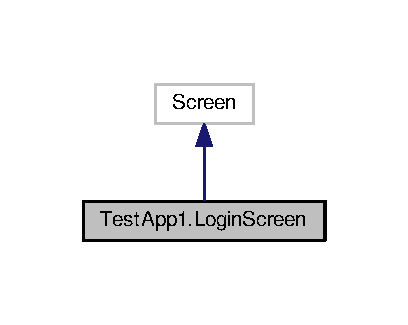
\includegraphics[width=196pt]{classTestApp1_1_1LoginScreen__inherit__graph}
\end{center}
\end{figure}


Collaboration diagram for Test\+App1.\+Login\+Screen\+:
\nopagebreak
\begin{figure}[H]
\begin{center}
\leavevmode
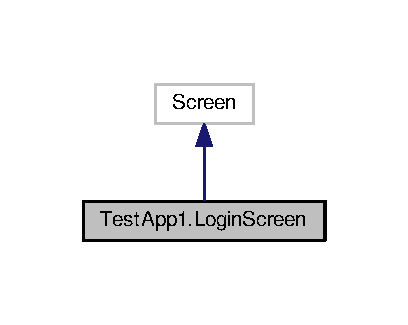
\includegraphics[width=196pt]{classTestApp1_1_1LoginScreen__coll__graph}
\end{center}
\end{figure}
\subsection*{Public Member Functions}
\begin{DoxyCompactItemize}
\item 
def \hyperlink{classTestApp1_1_1LoginScreen_a112fceb7785f8596158f842d5c223936}{login} (self, username, password)
\end{DoxyCompactItemize}
\subsection*{Static Public Attributes}
\begin{DoxyCompactItemize}
\item 
\hyperlink{classTestApp1_1_1LoginScreen_ad9ee7d178fec4c941960ebf2e5ce8239}{box} = Box\+Layout(orientation = \textquotesingle{}vertical\textquotesingle{}, padding = (5))
\item 
\hyperlink{classTestApp1_1_1LoginScreen_ab64836ea6220beb4d6141a08d1c1cdb6}{popup}
\end{DoxyCompactItemize}


\subsection{Member Function Documentation}
\index{Test\+App1\+::\+Login\+Screen@{Test\+App1\+::\+Login\+Screen}!login@{login}}
\index{login@{login}!Test\+App1\+::\+Login\+Screen@{Test\+App1\+::\+Login\+Screen}}
\subsubsection[{\texorpdfstring{login(self, username, password)}{login(self, username, password)}}]{\setlength{\rightskip}{0pt plus 5cm}def Test\+App1.\+Login\+Screen.\+login (
\begin{DoxyParamCaption}
\item[{}]{self, }
\item[{}]{username, }
\item[{}]{password}
\end{DoxyParamCaption}
)}\hypertarget{classTestApp1_1_1LoginScreen_a112fceb7785f8596158f842d5c223936}{}\label{classTestApp1_1_1LoginScreen_a112fceb7785f8596158f842d5c223936}


\subsection{Member Data Documentation}
\index{Test\+App1\+::\+Login\+Screen@{Test\+App1\+::\+Login\+Screen}!box@{box}}
\index{box@{box}!Test\+App1\+::\+Login\+Screen@{Test\+App1\+::\+Login\+Screen}}
\subsubsection[{\texorpdfstring{box}{box}}]{\setlength{\rightskip}{0pt plus 5cm}Test\+App1.\+Login\+Screen.\+box = Box\+Layout(orientation = \textquotesingle{}vertical\textquotesingle{}, padding = (5))\hspace{0.3cm}{\ttfamily [static]}}\hypertarget{classTestApp1_1_1LoginScreen_ad9ee7d178fec4c941960ebf2e5ce8239}{}\label{classTestApp1_1_1LoginScreen_ad9ee7d178fec4c941960ebf2e5ce8239}
\index{Test\+App1\+::\+Login\+Screen@{Test\+App1\+::\+Login\+Screen}!popup@{popup}}
\index{popup@{popup}!Test\+App1\+::\+Login\+Screen@{Test\+App1\+::\+Login\+Screen}}
\subsubsection[{\texorpdfstring{popup}{popup}}]{\setlength{\rightskip}{0pt plus 5cm}Test\+App1.\+Login\+Screen.\+popup\hspace{0.3cm}{\ttfamily [static]}}\hypertarget{classTestApp1_1_1LoginScreen_ab64836ea6220beb4d6141a08d1c1cdb6}{}\label{classTestApp1_1_1LoginScreen_ab64836ea6220beb4d6141a08d1c1cdb6}
{\bfseries Initial value\+:}
\begin{DoxyCode}
1 = Popup(title=\textcolor{stringliteral}{'Login Error'},
2                           title\_size =(30),title\_align=\textcolor{stringliteral}{'center'},
3                           content=box,size=(25,25),auto\_dismiss=\textcolor{keyword}{True})
\end{DoxyCode}


The documentation for this class was generated from the following file\+:\begin{DoxyCompactItemize}
\item 
/home/jac0656/\+Desktop/\+J-\/\+O-\/\+R-\/\+G-\/\+E/\+U\+N\+T-\/\+N\+A\+S\+A/\hyperlink{TestApp1_8py}{Test\+App1.\+py}\end{DoxyCompactItemize}

\hypertarget{classGUI8J_1_1LoginScreen}{}\section{G\+U\+I8\+J.\+Login\+Screen Class Reference}
\label{classGUI8J_1_1LoginScreen}\index{G\+U\+I8\+J.\+Login\+Screen@{G\+U\+I8\+J.\+Login\+Screen}}


Inheritance diagram for G\+U\+I8\+J.\+Login\+Screen\+:
% FIG 0


Collaboration diagram for G\+U\+I8\+J.\+Login\+Screen\+:
% FIG 1
\subsection*{Public Member Functions}
\begin{DoxyCompactItemize}
\item 
def \hyperlink{classGUI8J_1_1LoginScreen_adeed689e5c760bced0580e28839f5dc7}{login} (self, username, password)
\end{DoxyCompactItemize}


\subsection{Member Function Documentation}
\mbox{\Hypertarget{classGUI8J_1_1LoginScreen_adeed689e5c760bced0580e28839f5dc7}\label{classGUI8J_1_1LoginScreen_adeed689e5c760bced0580e28839f5dc7}} 
\index{G\+U\+I8\+J\+::\+Login\+Screen@{G\+U\+I8\+J\+::\+Login\+Screen}!login@{login}}
\index{login@{login}!G\+U\+I8\+J\+::\+Login\+Screen@{G\+U\+I8\+J\+::\+Login\+Screen}}
\subsubsection{\texorpdfstring{login()}{login()}}
{\footnotesize\ttfamily def G\+U\+I8\+J.\+Login\+Screen.\+login (\begin{DoxyParamCaption}\item[{}]{self,  }\item[{}]{username,  }\item[{}]{password }\end{DoxyParamCaption})}



The documentation for this class was generated from the following file\+:\begin{DoxyCompactItemize}
\item 
/home/pi/\+Desktop/\+U\+N\+T-\/\+N\+A\+S\+A/\+G\+U\+I/\hyperlink{GUI8J_8py}{G\+U\+I8\+J.\+py}\end{DoxyCompactItemize}

\hypertarget{classTestingGUI_1_1LoginScreen}{}\section{Testing\+G\+U\+I.\+Login\+Screen Class Reference}
\label{classTestingGUI_1_1LoginScreen}\index{Testing\+G\+U\+I.\+Login\+Screen@{Testing\+G\+U\+I.\+Login\+Screen}}


Inheritance diagram for Testing\+G\+U\+I.\+Login\+Screen\+:
\nopagebreak
\begin{figure}[H]
\begin{center}
\leavevmode
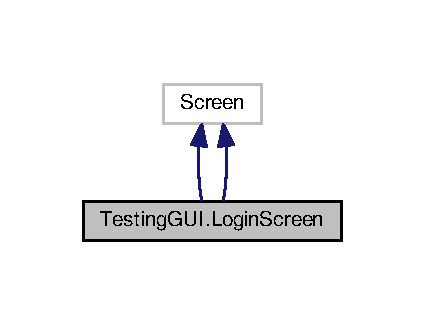
\includegraphics[width=204pt]{classTestingGUI_1_1LoginScreen__inherit__graph}
\end{center}
\end{figure}


Collaboration diagram for Testing\+G\+U\+I.\+Login\+Screen\+:
\nopagebreak
\begin{figure}[H]
\begin{center}
\leavevmode
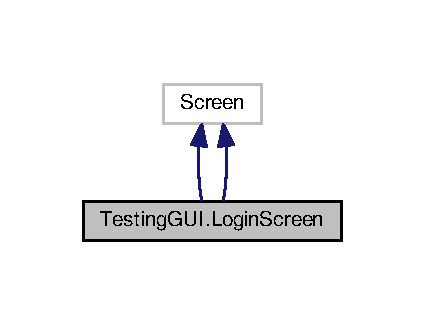
\includegraphics[width=204pt]{classTestingGUI_1_1LoginScreen__coll__graph}
\end{center}
\end{figure}
\subsection*{Public Member Functions}
\begin{DoxyCompactItemize}
\item 
def \hyperlink{classTestingGUI_1_1LoginScreen_a4a73599bf5eda0f45a27c541a6daf599}{login} (self, username, password)
\item 
def \hyperlink{classTestingGUI_1_1LoginScreen_a4a73599bf5eda0f45a27c541a6daf599}{login} (self, username, password)
\end{DoxyCompactItemize}


\subsection{Member Function Documentation}
\index{Testing\+G\+U\+I\+::\+Login\+Screen@{Testing\+G\+U\+I\+::\+Login\+Screen}!login@{login}}
\index{login@{login}!Testing\+G\+U\+I\+::\+Login\+Screen@{Testing\+G\+U\+I\+::\+Login\+Screen}}
\subsubsection[{\texorpdfstring{login(self, username, password)}{login(self, username, password)}}]{\setlength{\rightskip}{0pt plus 5cm}def Testing\+G\+U\+I.\+Login\+Screen.\+login (
\begin{DoxyParamCaption}
\item[{}]{self, }
\item[{}]{username, }
\item[{}]{password}
\end{DoxyParamCaption}
)}\hypertarget{classTestingGUI_1_1LoginScreen_a4a73599bf5eda0f45a27c541a6daf599}{}\label{classTestingGUI_1_1LoginScreen_a4a73599bf5eda0f45a27c541a6daf599}
\index{Testing\+G\+U\+I\+::\+Login\+Screen@{Testing\+G\+U\+I\+::\+Login\+Screen}!login@{login}}
\index{login@{login}!Testing\+G\+U\+I\+::\+Login\+Screen@{Testing\+G\+U\+I\+::\+Login\+Screen}}
\subsubsection[{\texorpdfstring{login(self, username, password)}{login(self, username, password)}}]{\setlength{\rightskip}{0pt plus 5cm}def Testing\+G\+U\+I.\+Login\+Screen.\+login (
\begin{DoxyParamCaption}
\item[{}]{self, }
\item[{}]{username, }
\item[{}]{password}
\end{DoxyParamCaption}
)}\hypertarget{classTestingGUI_1_1LoginScreen_a4a73599bf5eda0f45a27c541a6daf599}{}\label{classTestingGUI_1_1LoginScreen_a4a73599bf5eda0f45a27c541a6daf599}


The documentation for this class was generated from the following file\+:\begin{DoxyCompactItemize}
\item 
/home/jac0656/\+Desktop/\+J-\/\+O-\/\+R-\/\+G-\/\+E/\+U\+N\+T-\/\+N\+A\+S\+A/\+G\+U\+I/\hyperlink{GUI_2TestingGUI_8py}{Testing\+G\+U\+I.\+py}\end{DoxyCompactItemize}

\hypertarget{classGUI8-5pm_1_1LoginScreen}{}\section{G\+U\+I8-\/5pm.Login\+Screen Class Reference}
\label{classGUI8-5pm_1_1LoginScreen}\index{G\+U\+I8-\/5pm.\+Login\+Screen@{G\+U\+I8-\/5pm.\+Login\+Screen}}


Inheritance diagram for G\+U\+I8-\/5pm.Login\+Screen\+:
\nopagebreak
\begin{figure}[H]
\begin{center}
\leavevmode
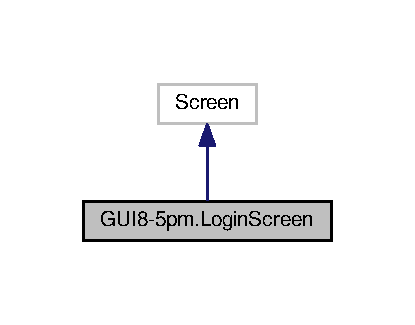
\includegraphics[width=199pt]{classGUI8-5pm_1_1LoginScreen__inherit__graph}
\end{center}
\end{figure}


Collaboration diagram for G\+U\+I8-\/5pm.Login\+Screen\+:
\nopagebreak
\begin{figure}[H]
\begin{center}
\leavevmode
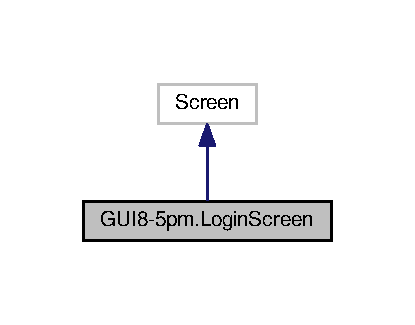
\includegraphics[width=199pt]{classGUI8-5pm_1_1LoginScreen__coll__graph}
\end{center}
\end{figure}
\subsection*{Public Member Functions}
\begin{DoxyCompactItemize}
\item 
def \hyperlink{classGUI8-5pm_1_1LoginScreen_a6a2491d7a12c5d815373aad6f4357b99}{login} (self, username, password)
\end{DoxyCompactItemize}


\subsection{Member Function Documentation}
\index{G\+U\+I8-\/5pm\+::\+Login\+Screen@{G\+U\+I8-\/5pm\+::\+Login\+Screen}!login@{login}}
\index{login@{login}!G\+U\+I8-\/5pm\+::\+Login\+Screen@{G\+U\+I8-\/5pm\+::\+Login\+Screen}}
\subsubsection[{\texorpdfstring{login(self, username, password)}{login(self, username, password)}}]{\setlength{\rightskip}{0pt plus 5cm}def G\+U\+I8-\/5pm.\+Login\+Screen.\+login (
\begin{DoxyParamCaption}
\item[{}]{self, }
\item[{}]{username, }
\item[{}]{password}
\end{DoxyParamCaption}
)}\hypertarget{classGUI8-5pm_1_1LoginScreen_a6a2491d7a12c5d815373aad6f4357b99}{}\label{classGUI8-5pm_1_1LoginScreen_a6a2491d7a12c5d815373aad6f4357b99}


The documentation for this class was generated from the following file\+:\begin{DoxyCompactItemize}
\item 
/home/jac0656/\+Desktop/\+J-\/\+O-\/\+R-\/\+G-\/\+E/\+U\+N\+T-\/\+N\+A\+S\+A/\hyperlink{GUI8-5pm_8py}{G\+U\+I8-\/5pm.\+py}\end{DoxyCompactItemize}

\hypertarget{classGUI8_1_1LoginScreen}{}\section{G\+U\+I8.\+Login\+Screen Class Reference}
\label{classGUI8_1_1LoginScreen}\index{G\+U\+I8.\+Login\+Screen@{G\+U\+I8.\+Login\+Screen}}


Inheritance diagram for G\+U\+I8.\+Login\+Screen\+:
\nopagebreak
\begin{figure}[H]
\begin{center}
\leavevmode
\includegraphics[width=177pt]{classGUI8_1_1LoginScreen__inherit__graph}
\end{center}
\end{figure}


Collaboration diagram for G\+U\+I8.\+Login\+Screen\+:
\nopagebreak
\begin{figure}[H]
\begin{center}
\leavevmode
\includegraphics[width=177pt]{classGUI8_1_1LoginScreen__coll__graph}
\end{center}
\end{figure}
\subsection*{Public Member Functions}
\begin{DoxyCompactItemize}
\item 
def \hyperlink{classGUI8_1_1LoginScreen_aeed2e30b7b40b78af0220e1800d898d7}{login} (self, username, password)
\item 
def \hyperlink{classGUI8_1_1LoginScreen_aeed2e30b7b40b78af0220e1800d898d7}{login} (self, username, password)
\end{DoxyCompactItemize}


\subsection{Member Function Documentation}
\index{G\+U\+I8\+::\+Login\+Screen@{G\+U\+I8\+::\+Login\+Screen}!login@{login}}
\index{login@{login}!G\+U\+I8\+::\+Login\+Screen@{G\+U\+I8\+::\+Login\+Screen}}
\subsubsection[{\texorpdfstring{login(self, username, password)}{login(self, username, password)}}]{\setlength{\rightskip}{0pt plus 5cm}def G\+U\+I8.\+Login\+Screen.\+login (
\begin{DoxyParamCaption}
\item[{}]{self, }
\item[{}]{username, }
\item[{}]{password}
\end{DoxyParamCaption}
)}\hypertarget{classGUI8_1_1LoginScreen_aeed2e30b7b40b78af0220e1800d898d7}{}\label{classGUI8_1_1LoginScreen_aeed2e30b7b40b78af0220e1800d898d7}
\index{G\+U\+I8\+::\+Login\+Screen@{G\+U\+I8\+::\+Login\+Screen}!login@{login}}
\index{login@{login}!G\+U\+I8\+::\+Login\+Screen@{G\+U\+I8\+::\+Login\+Screen}}
\subsubsection[{\texorpdfstring{login(self, username, password)}{login(self, username, password)}}]{\setlength{\rightskip}{0pt plus 5cm}def G\+U\+I8.\+Login\+Screen.\+login (
\begin{DoxyParamCaption}
\item[{}]{self, }
\item[{}]{username, }
\item[{}]{password}
\end{DoxyParamCaption}
)}\hypertarget{classGUI8_1_1LoginScreen_aeed2e30b7b40b78af0220e1800d898d7}{}\label{classGUI8_1_1LoginScreen_aeed2e30b7b40b78af0220e1800d898d7}


The documentation for this class was generated from the following file\+:\begin{DoxyCompactItemize}
\item 
/home/jac0656/\+Desktop/\+J-\/\+O-\/\+R-\/\+G-\/\+E/\+U\+N\+T-\/\+N\+A\+S\+A/\+G\+U\+I/\hyperlink{GUI_2GUI8_8py}{G\+U\+I8.\+py}\end{DoxyCompactItemize}

\hypertarget{classnewGUI_1_1LoginScreen}{}\section{new\+G\+U\+I.\+Login\+Screen Class Reference}
\label{classnewGUI_1_1LoginScreen}\index{new\+G\+U\+I.\+Login\+Screen@{new\+G\+U\+I.\+Login\+Screen}}


Inheritance diagram for new\+G\+U\+I.\+Login\+Screen\+:\nopagebreak
\begin{figure}[H]
\begin{center}
\leavevmode
\includegraphics[width=190pt]{classnewGUI_1_1LoginScreen__inherit__graph}
\end{center}
\end{figure}


Collaboration diagram for new\+G\+U\+I.\+Login\+Screen\+:\nopagebreak
\begin{figure}[H]
\begin{center}
\leavevmode
\includegraphics[width=190pt]{classnewGUI_1_1LoginScreen__coll__graph}
\end{center}
\end{figure}
\subsection*{Public Member Functions}
\begin{DoxyCompactItemize}
\item 
def \hyperlink{classnewGUI_1_1LoginScreen_afba0a3ad9779a11e63e36ac4ec20af6b}{login} (self, username, password)
\end{DoxyCompactItemize}


\subsection{Member Function Documentation}
\index{new\+G\+U\+I\+::\+Login\+Screen@{new\+G\+U\+I\+::\+Login\+Screen}!login@{login}}
\index{login@{login}!new\+G\+U\+I\+::\+Login\+Screen@{new\+G\+U\+I\+::\+Login\+Screen}}
\subsubsection[{\texorpdfstring{login(self, username, password)}{login(self, username, password)}}]{\setlength{\rightskip}{0pt plus 5cm}def new\+G\+U\+I.\+Login\+Screen.\+login (
\begin{DoxyParamCaption}
\item[{}]{self, }
\item[{}]{username, }
\item[{}]{password}
\end{DoxyParamCaption}
)}\hypertarget{classnewGUI_1_1LoginScreen_afba0a3ad9779a11e63e36ac4ec20af6b}{}\label{classnewGUI_1_1LoginScreen_afba0a3ad9779a11e63e36ac4ec20af6b}


The documentation for this class was generated from the following file\+:\begin{DoxyCompactItemize}
\item 
/home/jac0656/\+Desktop/\+J-\/\+O-\/\+R-\/\+G-\/\+E/\+U\+N\+T-\/\+N\+A\+S\+A/\+G\+U\+I/\hyperlink{newGUI_8py}{new\+G\+U\+I.\+py}\end{DoxyCompactItemize}

\hypertarget{classTestingGUI_1_1Methods}{}\section{Testing\+G\+U\+I.\+Methods Class Reference}
\label{classTestingGUI_1_1Methods}\index{Testing\+G\+U\+I.\+Methods@{Testing\+G\+U\+I.\+Methods}}


Inheritance diagram for Testing\+G\+U\+I.\+Methods\+:
\nopagebreak
\begin{figure}[H]
\begin{center}
\leavevmode
\includegraphics[width=187pt]{classTestingGUI_1_1Methods__inherit__graph}
\end{center}
\end{figure}


Collaboration diagram for Testing\+G\+U\+I.\+Methods\+:
\nopagebreak
\begin{figure}[H]
\begin{center}
\leavevmode
\includegraphics[width=187pt]{classTestingGUI_1_1Methods__coll__graph}
\end{center}
\end{figure}
\subsection*{Public Member Functions}
\begin{DoxyCompactItemize}
\item 
def \hyperlink{classTestingGUI_1_1Methods_a6b7453ea737e1e8b53e33f999d0c9f2a}{\+\_\+\+\_\+init\+\_\+\+\_\+} (self, kwargs)
\item 
def \hyperlink{classTestingGUI_1_1Methods_a7caae1065692f63bf28b64e8f7c0709b}{C\+R\+\_\+update\+\_\+\+A\+LL} (self)
\item 
def \hyperlink{classTestingGUI_1_1Methods_a9c1aa20eca768d36ff23c118e35052eb}{C\+R\+\_\+update} (self, ip\+\_\+addr)
\item 
def \hyperlink{classTestingGUI_1_1Methods_a0709231f5f6f33c59ce325c7e3ebf156}{update\+\_\+dict} (self)
\item 
def \hyperlink{classTestingGUI_1_1Methods_adcf75d9e2ac64426a6f46e7797d221c0}{remove\+Light} (self, ip\+\_\+address)
\item 
def \hyperlink{classTestingGUI_1_1Methods_a5313fe533c054cf6077aeb101de8e73b}{process\+\_\+cmd} (self, IP, function, any\+\_\+data)
\item 
def \hyperlink{classTestingGUI_1_1Methods_aefc0f91f471aeef7ee76a5ad85ad8afc}{cmdparser} (self)
\item 
def \hyperlink{classTestingGUI_1_1Methods_a6b7453ea737e1e8b53e33f999d0c9f2a}{\+\_\+\+\_\+init\+\_\+\+\_\+} (self, kwargs)
\item 
def \hyperlink{classTestingGUI_1_1Methods_a7caae1065692f63bf28b64e8f7c0709b}{C\+R\+\_\+update\+\_\+\+A\+LL} (self)
\item 
def \hyperlink{classTestingGUI_1_1Methods_a9c1aa20eca768d36ff23c118e35052eb}{C\+R\+\_\+update} (self, ip\+\_\+addr)
\item 
def \hyperlink{classTestingGUI_1_1Methods_a0709231f5f6f33c59ce325c7e3ebf156}{update\+\_\+dict} (self)
\item 
def \hyperlink{classTestingGUI_1_1Methods_adcf75d9e2ac64426a6f46e7797d221c0}{remove\+Light} (self, ip\+\_\+address)
\item 
def \hyperlink{classTestingGUI_1_1Methods_a5313fe533c054cf6077aeb101de8e73b}{process\+\_\+cmd} (self, IP, function, any\+\_\+data)
\item 
def \hyperlink{classTestingGUI_1_1Methods_aefc0f91f471aeef7ee76a5ad85ad8afc}{cmdparser} (self)
\item 
def \hyperlink{classTestingGUI_1_1Methods_a6b7453ea737e1e8b53e33f999d0c9f2a}{\+\_\+\+\_\+init\+\_\+\+\_\+} (self, kwargs)
\item 
def \hyperlink{classTestingGUI_1_1Methods_a7caae1065692f63bf28b64e8f7c0709b}{C\+R\+\_\+update\+\_\+\+A\+LL} (self)
\item 
def \hyperlink{classTestingGUI_1_1Methods_a9c1aa20eca768d36ff23c118e35052eb}{C\+R\+\_\+update} (self, ip\+\_\+addr)
\item 
def \hyperlink{classTestingGUI_1_1Methods_a0709231f5f6f33c59ce325c7e3ebf156}{update\+\_\+dict} (self)
\item 
def \hyperlink{classTestingGUI_1_1Methods_adcf75d9e2ac64426a6f46e7797d221c0}{remove\+Light} (self, ip\+\_\+address)
\item 
def \hyperlink{classTestingGUI_1_1Methods_a5313fe533c054cf6077aeb101de8e73b}{process\+\_\+cmd} (self, IP, function, any\+\_\+data)
\item 
def \hyperlink{classTestingGUI_1_1Methods_aefc0f91f471aeef7ee76a5ad85ad8afc}{cmdparser} (self)
\end{DoxyCompactItemize}


\subsection{Constructor \& Destructor Documentation}
\index{Testing\+G\+U\+I\+::\+Methods@{Testing\+G\+U\+I\+::\+Methods}!\+\_\+\+\_\+init\+\_\+\+\_\+@{\+\_\+\+\_\+init\+\_\+\+\_\+}}
\index{\+\_\+\+\_\+init\+\_\+\+\_\+@{\+\_\+\+\_\+init\+\_\+\+\_\+}!Testing\+G\+U\+I\+::\+Methods@{Testing\+G\+U\+I\+::\+Methods}}
\subsubsection[{\texorpdfstring{\+\_\+\+\_\+init\+\_\+\+\_\+(self, kwargs)}{__init__(self, kwargs)}}]{\setlength{\rightskip}{0pt plus 5cm}def Testing\+G\+U\+I.\+Methods.\+\_\+\+\_\+init\+\_\+\+\_\+ (
\begin{DoxyParamCaption}
\item[{}]{self, }
\item[{}]{kwargs}
\end{DoxyParamCaption}
)}\hypertarget{classTestingGUI_1_1Methods_a6b7453ea737e1e8b53e33f999d0c9f2a}{}\label{classTestingGUI_1_1Methods_a6b7453ea737e1e8b53e33f999d0c9f2a}
\index{Testing\+G\+U\+I\+::\+Methods@{Testing\+G\+U\+I\+::\+Methods}!\+\_\+\+\_\+init\+\_\+\+\_\+@{\+\_\+\+\_\+init\+\_\+\+\_\+}}
\index{\+\_\+\+\_\+init\+\_\+\+\_\+@{\+\_\+\+\_\+init\+\_\+\+\_\+}!Testing\+G\+U\+I\+::\+Methods@{Testing\+G\+U\+I\+::\+Methods}}
\subsubsection[{\texorpdfstring{\+\_\+\+\_\+init\+\_\+\+\_\+(self, kwargs)}{__init__(self, kwargs)}}]{\setlength{\rightskip}{0pt plus 5cm}def Testing\+G\+U\+I.\+Methods.\+\_\+\+\_\+init\+\_\+\+\_\+ (
\begin{DoxyParamCaption}
\item[{}]{self, }
\item[{}]{kwargs}
\end{DoxyParamCaption}
)}\hypertarget{classTestingGUI_1_1Methods_a6b7453ea737e1e8b53e33f999d0c9f2a}{}\label{classTestingGUI_1_1Methods_a6b7453ea737e1e8b53e33f999d0c9f2a}
\index{Testing\+G\+U\+I\+::\+Methods@{Testing\+G\+U\+I\+::\+Methods}!\+\_\+\+\_\+init\+\_\+\+\_\+@{\+\_\+\+\_\+init\+\_\+\+\_\+}}
\index{\+\_\+\+\_\+init\+\_\+\+\_\+@{\+\_\+\+\_\+init\+\_\+\+\_\+}!Testing\+G\+U\+I\+::\+Methods@{Testing\+G\+U\+I\+::\+Methods}}
\subsubsection[{\texorpdfstring{\+\_\+\+\_\+init\+\_\+\+\_\+(self, kwargs)}{__init__(self, kwargs)}}]{\setlength{\rightskip}{0pt plus 5cm}def Testing\+G\+U\+I.\+Methods.\+\_\+\+\_\+init\+\_\+\+\_\+ (
\begin{DoxyParamCaption}
\item[{}]{self, }
\item[{}]{kwargs}
\end{DoxyParamCaption}
)}\hypertarget{classTestingGUI_1_1Methods_a6b7453ea737e1e8b53e33f999d0c9f2a}{}\label{classTestingGUI_1_1Methods_a6b7453ea737e1e8b53e33f999d0c9f2a}


\subsection{Member Function Documentation}
\index{Testing\+G\+U\+I\+::\+Methods@{Testing\+G\+U\+I\+::\+Methods}!cmdparser@{cmdparser}}
\index{cmdparser@{cmdparser}!Testing\+G\+U\+I\+::\+Methods@{Testing\+G\+U\+I\+::\+Methods}}
\subsubsection[{\texorpdfstring{cmdparser(self)}{cmdparser(self)}}]{\setlength{\rightskip}{0pt plus 5cm}def Testing\+G\+U\+I.\+Methods.\+cmdparser (
\begin{DoxyParamCaption}
\item[{}]{self}
\end{DoxyParamCaption}
)}\hypertarget{classTestingGUI_1_1Methods_aefc0f91f471aeef7ee76a5ad85ad8afc}{}\label{classTestingGUI_1_1Methods_aefc0f91f471aeef7ee76a5ad85ad8afc}
\index{Testing\+G\+U\+I\+::\+Methods@{Testing\+G\+U\+I\+::\+Methods}!cmdparser@{cmdparser}}
\index{cmdparser@{cmdparser}!Testing\+G\+U\+I\+::\+Methods@{Testing\+G\+U\+I\+::\+Methods}}
\subsubsection[{\texorpdfstring{cmdparser(self)}{cmdparser(self)}}]{\setlength{\rightskip}{0pt plus 5cm}def Testing\+G\+U\+I.\+Methods.\+cmdparser (
\begin{DoxyParamCaption}
\item[{}]{self}
\end{DoxyParamCaption}
)}\hypertarget{classTestingGUI_1_1Methods_aefc0f91f471aeef7ee76a5ad85ad8afc}{}\label{classTestingGUI_1_1Methods_aefc0f91f471aeef7ee76a5ad85ad8afc}
\index{Testing\+G\+U\+I\+::\+Methods@{Testing\+G\+U\+I\+::\+Methods}!cmdparser@{cmdparser}}
\index{cmdparser@{cmdparser}!Testing\+G\+U\+I\+::\+Methods@{Testing\+G\+U\+I\+::\+Methods}}
\subsubsection[{\texorpdfstring{cmdparser(self)}{cmdparser(self)}}]{\setlength{\rightskip}{0pt plus 5cm}def Testing\+G\+U\+I.\+Methods.\+cmdparser (
\begin{DoxyParamCaption}
\item[{}]{self}
\end{DoxyParamCaption}
)}\hypertarget{classTestingGUI_1_1Methods_aefc0f91f471aeef7ee76a5ad85ad8afc}{}\label{classTestingGUI_1_1Methods_aefc0f91f471aeef7ee76a5ad85ad8afc}
\index{Testing\+G\+U\+I\+::\+Methods@{Testing\+G\+U\+I\+::\+Methods}!C\+R\+\_\+update@{C\+R\+\_\+update}}
\index{C\+R\+\_\+update@{C\+R\+\_\+update}!Testing\+G\+U\+I\+::\+Methods@{Testing\+G\+U\+I\+::\+Methods}}
\subsubsection[{\texorpdfstring{C\+R\+\_\+update(self, ip\+\_\+addr)}{CR_update(self, ip_addr)}}]{\setlength{\rightskip}{0pt plus 5cm}def Testing\+G\+U\+I.\+Methods.\+C\+R\+\_\+update (
\begin{DoxyParamCaption}
\item[{}]{self, }
\item[{}]{ip\+\_\+addr}
\end{DoxyParamCaption}
)}\hypertarget{classTestingGUI_1_1Methods_a9c1aa20eca768d36ff23c118e35052eb}{}\label{classTestingGUI_1_1Methods_a9c1aa20eca768d36ff23c118e35052eb}
\index{Testing\+G\+U\+I\+::\+Methods@{Testing\+G\+U\+I\+::\+Methods}!C\+R\+\_\+update@{C\+R\+\_\+update}}
\index{C\+R\+\_\+update@{C\+R\+\_\+update}!Testing\+G\+U\+I\+::\+Methods@{Testing\+G\+U\+I\+::\+Methods}}
\subsubsection[{\texorpdfstring{C\+R\+\_\+update(self, ip\+\_\+addr)}{CR_update(self, ip_addr)}}]{\setlength{\rightskip}{0pt plus 5cm}def Testing\+G\+U\+I.\+Methods.\+C\+R\+\_\+update (
\begin{DoxyParamCaption}
\item[{}]{self, }
\item[{}]{ip\+\_\+addr}
\end{DoxyParamCaption}
)}\hypertarget{classTestingGUI_1_1Methods_a9c1aa20eca768d36ff23c118e35052eb}{}\label{classTestingGUI_1_1Methods_a9c1aa20eca768d36ff23c118e35052eb}
\index{Testing\+G\+U\+I\+::\+Methods@{Testing\+G\+U\+I\+::\+Methods}!C\+R\+\_\+update@{C\+R\+\_\+update}}
\index{C\+R\+\_\+update@{C\+R\+\_\+update}!Testing\+G\+U\+I\+::\+Methods@{Testing\+G\+U\+I\+::\+Methods}}
\subsubsection[{\texorpdfstring{C\+R\+\_\+update(self, ip\+\_\+addr)}{CR_update(self, ip_addr)}}]{\setlength{\rightskip}{0pt plus 5cm}def Testing\+G\+U\+I.\+Methods.\+C\+R\+\_\+update (
\begin{DoxyParamCaption}
\item[{}]{self, }
\item[{}]{ip\+\_\+addr}
\end{DoxyParamCaption}
)}\hypertarget{classTestingGUI_1_1Methods_a9c1aa20eca768d36ff23c118e35052eb}{}\label{classTestingGUI_1_1Methods_a9c1aa20eca768d36ff23c118e35052eb}
\index{Testing\+G\+U\+I\+::\+Methods@{Testing\+G\+U\+I\+::\+Methods}!C\+R\+\_\+update\+\_\+\+A\+LL@{C\+R\+\_\+update\+\_\+\+A\+LL}}
\index{C\+R\+\_\+update\+\_\+\+A\+LL@{C\+R\+\_\+update\+\_\+\+A\+LL}!Testing\+G\+U\+I\+::\+Methods@{Testing\+G\+U\+I\+::\+Methods}}
\subsubsection[{\texorpdfstring{C\+R\+\_\+update\+\_\+\+A\+L\+L(self)}{CR_update_ALL(self)}}]{\setlength{\rightskip}{0pt plus 5cm}def Testing\+G\+U\+I.\+Methods.\+C\+R\+\_\+update\+\_\+\+A\+LL (
\begin{DoxyParamCaption}
\item[{}]{self}
\end{DoxyParamCaption}
)}\hypertarget{classTestingGUI_1_1Methods_a7caae1065692f63bf28b64e8f7c0709b}{}\label{classTestingGUI_1_1Methods_a7caae1065692f63bf28b64e8f7c0709b}
\index{Testing\+G\+U\+I\+::\+Methods@{Testing\+G\+U\+I\+::\+Methods}!C\+R\+\_\+update\+\_\+\+A\+LL@{C\+R\+\_\+update\+\_\+\+A\+LL}}
\index{C\+R\+\_\+update\+\_\+\+A\+LL@{C\+R\+\_\+update\+\_\+\+A\+LL}!Testing\+G\+U\+I\+::\+Methods@{Testing\+G\+U\+I\+::\+Methods}}
\subsubsection[{\texorpdfstring{C\+R\+\_\+update\+\_\+\+A\+L\+L(self)}{CR_update_ALL(self)}}]{\setlength{\rightskip}{0pt plus 5cm}def Testing\+G\+U\+I.\+Methods.\+C\+R\+\_\+update\+\_\+\+A\+LL (
\begin{DoxyParamCaption}
\item[{}]{self}
\end{DoxyParamCaption}
)}\hypertarget{classTestingGUI_1_1Methods_a7caae1065692f63bf28b64e8f7c0709b}{}\label{classTestingGUI_1_1Methods_a7caae1065692f63bf28b64e8f7c0709b}
\index{Testing\+G\+U\+I\+::\+Methods@{Testing\+G\+U\+I\+::\+Methods}!C\+R\+\_\+update\+\_\+\+A\+LL@{C\+R\+\_\+update\+\_\+\+A\+LL}}
\index{C\+R\+\_\+update\+\_\+\+A\+LL@{C\+R\+\_\+update\+\_\+\+A\+LL}!Testing\+G\+U\+I\+::\+Methods@{Testing\+G\+U\+I\+::\+Methods}}
\subsubsection[{\texorpdfstring{C\+R\+\_\+update\+\_\+\+A\+L\+L(self)}{CR_update_ALL(self)}}]{\setlength{\rightskip}{0pt plus 5cm}def Testing\+G\+U\+I.\+Methods.\+C\+R\+\_\+update\+\_\+\+A\+LL (
\begin{DoxyParamCaption}
\item[{}]{self}
\end{DoxyParamCaption}
)}\hypertarget{classTestingGUI_1_1Methods_a7caae1065692f63bf28b64e8f7c0709b}{}\label{classTestingGUI_1_1Methods_a7caae1065692f63bf28b64e8f7c0709b}
\index{Testing\+G\+U\+I\+::\+Methods@{Testing\+G\+U\+I\+::\+Methods}!process\+\_\+cmd@{process\+\_\+cmd}}
\index{process\+\_\+cmd@{process\+\_\+cmd}!Testing\+G\+U\+I\+::\+Methods@{Testing\+G\+U\+I\+::\+Methods}}
\subsubsection[{\texorpdfstring{process\+\_\+cmd(self, I\+P, function, any\+\_\+data)}{process_cmd(self, IP, function, any_data)}}]{\setlength{\rightskip}{0pt plus 5cm}def Testing\+G\+U\+I.\+Methods.\+process\+\_\+cmd (
\begin{DoxyParamCaption}
\item[{}]{self, }
\item[{}]{IP, }
\item[{}]{function, }
\item[{}]{any\+\_\+data}
\end{DoxyParamCaption}
)}\hypertarget{classTestingGUI_1_1Methods_a5313fe533c054cf6077aeb101de8e73b}{}\label{classTestingGUI_1_1Methods_a5313fe533c054cf6077aeb101de8e73b}
\index{Testing\+G\+U\+I\+::\+Methods@{Testing\+G\+U\+I\+::\+Methods}!process\+\_\+cmd@{process\+\_\+cmd}}
\index{process\+\_\+cmd@{process\+\_\+cmd}!Testing\+G\+U\+I\+::\+Methods@{Testing\+G\+U\+I\+::\+Methods}}
\subsubsection[{\texorpdfstring{process\+\_\+cmd(self, I\+P, function, any\+\_\+data)}{process_cmd(self, IP, function, any_data)}}]{\setlength{\rightskip}{0pt plus 5cm}def Testing\+G\+U\+I.\+Methods.\+process\+\_\+cmd (
\begin{DoxyParamCaption}
\item[{}]{self, }
\item[{}]{IP, }
\item[{}]{function, }
\item[{}]{any\+\_\+data}
\end{DoxyParamCaption}
)}\hypertarget{classTestingGUI_1_1Methods_a5313fe533c054cf6077aeb101de8e73b}{}\label{classTestingGUI_1_1Methods_a5313fe533c054cf6077aeb101de8e73b}
\index{Testing\+G\+U\+I\+::\+Methods@{Testing\+G\+U\+I\+::\+Methods}!process\+\_\+cmd@{process\+\_\+cmd}}
\index{process\+\_\+cmd@{process\+\_\+cmd}!Testing\+G\+U\+I\+::\+Methods@{Testing\+G\+U\+I\+::\+Methods}}
\subsubsection[{\texorpdfstring{process\+\_\+cmd(self, I\+P, function, any\+\_\+data)}{process_cmd(self, IP, function, any_data)}}]{\setlength{\rightskip}{0pt plus 5cm}def Testing\+G\+U\+I.\+Methods.\+process\+\_\+cmd (
\begin{DoxyParamCaption}
\item[{}]{self, }
\item[{}]{IP, }
\item[{}]{function, }
\item[{}]{any\+\_\+data}
\end{DoxyParamCaption}
)}\hypertarget{classTestingGUI_1_1Methods_a5313fe533c054cf6077aeb101de8e73b}{}\label{classTestingGUI_1_1Methods_a5313fe533c054cf6077aeb101de8e73b}
\index{Testing\+G\+U\+I\+::\+Methods@{Testing\+G\+U\+I\+::\+Methods}!remove\+Light@{remove\+Light}}
\index{remove\+Light@{remove\+Light}!Testing\+G\+U\+I\+::\+Methods@{Testing\+G\+U\+I\+::\+Methods}}
\subsubsection[{\texorpdfstring{remove\+Light(self, ip\+\_\+address)}{removeLight(self, ip_address)}}]{\setlength{\rightskip}{0pt plus 5cm}def Testing\+G\+U\+I.\+Methods.\+remove\+Light (
\begin{DoxyParamCaption}
\item[{}]{self, }
\item[{}]{ip\+\_\+address}
\end{DoxyParamCaption}
)}\hypertarget{classTestingGUI_1_1Methods_adcf75d9e2ac64426a6f46e7797d221c0}{}\label{classTestingGUI_1_1Methods_adcf75d9e2ac64426a6f46e7797d221c0}
\index{Testing\+G\+U\+I\+::\+Methods@{Testing\+G\+U\+I\+::\+Methods}!remove\+Light@{remove\+Light}}
\index{remove\+Light@{remove\+Light}!Testing\+G\+U\+I\+::\+Methods@{Testing\+G\+U\+I\+::\+Methods}}
\subsubsection[{\texorpdfstring{remove\+Light(self, ip\+\_\+address)}{removeLight(self, ip_address)}}]{\setlength{\rightskip}{0pt plus 5cm}def Testing\+G\+U\+I.\+Methods.\+remove\+Light (
\begin{DoxyParamCaption}
\item[{}]{self, }
\item[{}]{ip\+\_\+address}
\end{DoxyParamCaption}
)}\hypertarget{classTestingGUI_1_1Methods_adcf75d9e2ac64426a6f46e7797d221c0}{}\label{classTestingGUI_1_1Methods_adcf75d9e2ac64426a6f46e7797d221c0}
\index{Testing\+G\+U\+I\+::\+Methods@{Testing\+G\+U\+I\+::\+Methods}!remove\+Light@{remove\+Light}}
\index{remove\+Light@{remove\+Light}!Testing\+G\+U\+I\+::\+Methods@{Testing\+G\+U\+I\+::\+Methods}}
\subsubsection[{\texorpdfstring{remove\+Light(self, ip\+\_\+address)}{removeLight(self, ip_address)}}]{\setlength{\rightskip}{0pt plus 5cm}def Testing\+G\+U\+I.\+Methods.\+remove\+Light (
\begin{DoxyParamCaption}
\item[{}]{self, }
\item[{}]{ip\+\_\+address}
\end{DoxyParamCaption}
)}\hypertarget{classTestingGUI_1_1Methods_adcf75d9e2ac64426a6f46e7797d221c0}{}\label{classTestingGUI_1_1Methods_adcf75d9e2ac64426a6f46e7797d221c0}
\index{Testing\+G\+U\+I\+::\+Methods@{Testing\+G\+U\+I\+::\+Methods}!update\+\_\+dict@{update\+\_\+dict}}
\index{update\+\_\+dict@{update\+\_\+dict}!Testing\+G\+U\+I\+::\+Methods@{Testing\+G\+U\+I\+::\+Methods}}
\subsubsection[{\texorpdfstring{update\+\_\+dict(self)}{update_dict(self)}}]{\setlength{\rightskip}{0pt plus 5cm}def Testing\+G\+U\+I.\+Methods.\+update\+\_\+dict (
\begin{DoxyParamCaption}
\item[{}]{self}
\end{DoxyParamCaption}
)}\hypertarget{classTestingGUI_1_1Methods_a0709231f5f6f33c59ce325c7e3ebf156}{}\label{classTestingGUI_1_1Methods_a0709231f5f6f33c59ce325c7e3ebf156}
\index{Testing\+G\+U\+I\+::\+Methods@{Testing\+G\+U\+I\+::\+Methods}!update\+\_\+dict@{update\+\_\+dict}}
\index{update\+\_\+dict@{update\+\_\+dict}!Testing\+G\+U\+I\+::\+Methods@{Testing\+G\+U\+I\+::\+Methods}}
\subsubsection[{\texorpdfstring{update\+\_\+dict(self)}{update_dict(self)}}]{\setlength{\rightskip}{0pt plus 5cm}def Testing\+G\+U\+I.\+Methods.\+update\+\_\+dict (
\begin{DoxyParamCaption}
\item[{}]{self}
\end{DoxyParamCaption}
)}\hypertarget{classTestingGUI_1_1Methods_a0709231f5f6f33c59ce325c7e3ebf156}{}\label{classTestingGUI_1_1Methods_a0709231f5f6f33c59ce325c7e3ebf156}
\index{Testing\+G\+U\+I\+::\+Methods@{Testing\+G\+U\+I\+::\+Methods}!update\+\_\+dict@{update\+\_\+dict}}
\index{update\+\_\+dict@{update\+\_\+dict}!Testing\+G\+U\+I\+::\+Methods@{Testing\+G\+U\+I\+::\+Methods}}
\subsubsection[{\texorpdfstring{update\+\_\+dict(self)}{update_dict(self)}}]{\setlength{\rightskip}{0pt plus 5cm}def Testing\+G\+U\+I.\+Methods.\+update\+\_\+dict (
\begin{DoxyParamCaption}
\item[{}]{self}
\end{DoxyParamCaption}
)}\hypertarget{classTestingGUI_1_1Methods_a0709231f5f6f33c59ce325c7e3ebf156}{}\label{classTestingGUI_1_1Methods_a0709231f5f6f33c59ce325c7e3ebf156}


The documentation for this class was generated from the following file\+:\begin{DoxyCompactItemize}
\item 
/home/jac0656/\+Desktop/\+J-\/\+O-\/\+R-\/\+G-\/\+E/\+U\+N\+T-\/\+N\+A\+S\+A/\+G\+U\+I/\hyperlink{GUI_2TestingGUI_8py}{Testing\+G\+U\+I.\+py}\end{DoxyCompactItemize}

\hypertarget{classGUI8-5pm_1_1Methods}{}\section{G\+U\+I8-\/5pm.Methods Class Reference}
\label{classGUI8-5pm_1_1Methods}\index{G\+U\+I8-\/5pm.\+Methods@{G\+U\+I8-\/5pm.\+Methods}}


Inheritance diagram for G\+U\+I8-\/5pm.Methods\+:
\nopagebreak
\begin{figure}[H]
\begin{center}
\leavevmode
\includegraphics[width=182pt]{classGUI8-5pm_1_1Methods__inherit__graph}
\end{center}
\end{figure}


Collaboration diagram for G\+U\+I8-\/5pm.Methods\+:
\nopagebreak
\begin{figure}[H]
\begin{center}
\leavevmode
\includegraphics[width=182pt]{classGUI8-5pm_1_1Methods__coll__graph}
\end{center}
\end{figure}
\subsection*{Public Member Functions}
\begin{DoxyCompactItemize}
\item 
def \hyperlink{classGUI8-5pm_1_1Methods_ad3d84ecaf12cef3229179b6e4a7497f0}{\+\_\+\+\_\+init\+\_\+\+\_\+} (self, kwargs)
\item 
def \hyperlink{classGUI8-5pm_1_1Methods_a798c0b045c52f3791e186dcf7b086aa3}{build} (self, ip\+\_\+addr, t\+\_\+data)
\item 
def \hyperlink{classGUI8-5pm_1_1Methods_a474ca31dcf6413c7b3d8800d1729d79e}{store\+\_\+name} (self, arg1)
\item 
def \hyperlink{classGUI8-5pm_1_1Methods_a7d6fe3c2575dab4560aeafe69a36d910}{update\+\_\+lights} (self)
\item 
def \hyperlink{classGUI8-5pm_1_1Methods_acc36f5fc1abad09a81114d9ff9a19ff7}{update\+\_\+new\+\_\+light} (self, ip\+\_\+addr)
\item 
def \hyperlink{classGUI8-5pm_1_1Methods_a303853ed430eaff9bc4d16a0431c266f}{process\+\_\+cmd} (self, IP, function, any\+\_\+data)
\item 
def \hyperlink{classGUI8-5pm_1_1Methods_a4e22ae305d81d2519d6b9c58073f0574}{cmdparser} (self)
\end{DoxyCompactItemize}
\subsection*{Public Attributes}
\begin{DoxyCompactItemize}
\item 
\hyperlink{classGUI8-5pm_1_1Methods_ae5272965fe06cade1712f5c2db307f14}{textinput}
\end{DoxyCompactItemize}
\subsection*{Static Public Attributes}
\begin{DoxyCompactItemize}
\item 
string \hyperlink{classGUI8-5pm_1_1Methods_a6aab21b5537f2d0ab7e6bf6d9a7aa96b}{keyN} = \textquotesingle{}\textquotesingle{}
\item 
string \hyperlink{classGUI8-5pm_1_1Methods_a598aeed025ae6e48d199e7d9949b3e0a}{ip} = \textquotesingle{}\textquotesingle{}
\item 
string \hyperlink{classGUI8-5pm_1_1Methods_aa649f4722a90b2d0750727fcabf29236}{data} = \textquotesingle{}\textquotesingle{}
\end{DoxyCompactItemize}


\subsection{Constructor \& Destructor Documentation}
\index{G\+U\+I8-\/5pm\+::\+Methods@{G\+U\+I8-\/5pm\+::\+Methods}!\+\_\+\+\_\+init\+\_\+\+\_\+@{\+\_\+\+\_\+init\+\_\+\+\_\+}}
\index{\+\_\+\+\_\+init\+\_\+\+\_\+@{\+\_\+\+\_\+init\+\_\+\+\_\+}!G\+U\+I8-\/5pm\+::\+Methods@{G\+U\+I8-\/5pm\+::\+Methods}}
\subsubsection[{\texorpdfstring{\+\_\+\+\_\+init\+\_\+\+\_\+(self, kwargs)}{__init__(self, kwargs)}}]{\setlength{\rightskip}{0pt plus 5cm}def G\+U\+I8-\/5pm.\+Methods.\+\_\+\+\_\+init\+\_\+\+\_\+ (
\begin{DoxyParamCaption}
\item[{}]{self, }
\item[{}]{kwargs}
\end{DoxyParamCaption}
)}\hypertarget{classGUI8-5pm_1_1Methods_ad3d84ecaf12cef3229179b6e4a7497f0}{}\label{classGUI8-5pm_1_1Methods_ad3d84ecaf12cef3229179b6e4a7497f0}


\subsection{Member Function Documentation}
\index{G\+U\+I8-\/5pm\+::\+Methods@{G\+U\+I8-\/5pm\+::\+Methods}!build@{build}}
\index{build@{build}!G\+U\+I8-\/5pm\+::\+Methods@{G\+U\+I8-\/5pm\+::\+Methods}}
\subsubsection[{\texorpdfstring{build(self, ip\+\_\+addr, t\+\_\+data)}{build(self, ip_addr, t_data)}}]{\setlength{\rightskip}{0pt plus 5cm}def G\+U\+I8-\/5pm.\+Methods.\+build (
\begin{DoxyParamCaption}
\item[{}]{self, }
\item[{}]{ip\+\_\+addr, }
\item[{}]{t\+\_\+data}
\end{DoxyParamCaption}
)}\hypertarget{classGUI8-5pm_1_1Methods_a798c0b045c52f3791e186dcf7b086aa3}{}\label{classGUI8-5pm_1_1Methods_a798c0b045c52f3791e186dcf7b086aa3}
\index{G\+U\+I8-\/5pm\+::\+Methods@{G\+U\+I8-\/5pm\+::\+Methods}!cmdparser@{cmdparser}}
\index{cmdparser@{cmdparser}!G\+U\+I8-\/5pm\+::\+Methods@{G\+U\+I8-\/5pm\+::\+Methods}}
\subsubsection[{\texorpdfstring{cmdparser(self)}{cmdparser(self)}}]{\setlength{\rightskip}{0pt plus 5cm}def G\+U\+I8-\/5pm.\+Methods.\+cmdparser (
\begin{DoxyParamCaption}
\item[{}]{self}
\end{DoxyParamCaption}
)}\hypertarget{classGUI8-5pm_1_1Methods_a4e22ae305d81d2519d6b9c58073f0574}{}\label{classGUI8-5pm_1_1Methods_a4e22ae305d81d2519d6b9c58073f0574}
\index{G\+U\+I8-\/5pm\+::\+Methods@{G\+U\+I8-\/5pm\+::\+Methods}!process\+\_\+cmd@{process\+\_\+cmd}}
\index{process\+\_\+cmd@{process\+\_\+cmd}!G\+U\+I8-\/5pm\+::\+Methods@{G\+U\+I8-\/5pm\+::\+Methods}}
\subsubsection[{\texorpdfstring{process\+\_\+cmd(self, I\+P, function, any\+\_\+data)}{process_cmd(self, IP, function, any_data)}}]{\setlength{\rightskip}{0pt plus 5cm}def G\+U\+I8-\/5pm.\+Methods.\+process\+\_\+cmd (
\begin{DoxyParamCaption}
\item[{}]{self, }
\item[{}]{IP, }
\item[{}]{function, }
\item[{}]{any\+\_\+data}
\end{DoxyParamCaption}
)}\hypertarget{classGUI8-5pm_1_1Methods_a303853ed430eaff9bc4d16a0431c266f}{}\label{classGUI8-5pm_1_1Methods_a303853ed430eaff9bc4d16a0431c266f}
\index{G\+U\+I8-\/5pm\+::\+Methods@{G\+U\+I8-\/5pm\+::\+Methods}!store\+\_\+name@{store\+\_\+name}}
\index{store\+\_\+name@{store\+\_\+name}!G\+U\+I8-\/5pm\+::\+Methods@{G\+U\+I8-\/5pm\+::\+Methods}}
\subsubsection[{\texorpdfstring{store\+\_\+name(self, arg1)}{store_name(self, arg1)}}]{\setlength{\rightskip}{0pt plus 5cm}def G\+U\+I8-\/5pm.\+Methods.\+store\+\_\+name (
\begin{DoxyParamCaption}
\item[{}]{self, }
\item[{}]{arg1}
\end{DoxyParamCaption}
)}\hypertarget{classGUI8-5pm_1_1Methods_a474ca31dcf6413c7b3d8800d1729d79e}{}\label{classGUI8-5pm_1_1Methods_a474ca31dcf6413c7b3d8800d1729d79e}
\index{G\+U\+I8-\/5pm\+::\+Methods@{G\+U\+I8-\/5pm\+::\+Methods}!update\+\_\+lights@{update\+\_\+lights}}
\index{update\+\_\+lights@{update\+\_\+lights}!G\+U\+I8-\/5pm\+::\+Methods@{G\+U\+I8-\/5pm\+::\+Methods}}
\subsubsection[{\texorpdfstring{update\+\_\+lights(self)}{update_lights(self)}}]{\setlength{\rightskip}{0pt plus 5cm}def G\+U\+I8-\/5pm.\+Methods.\+update\+\_\+lights (
\begin{DoxyParamCaption}
\item[{}]{self}
\end{DoxyParamCaption}
)}\hypertarget{classGUI8-5pm_1_1Methods_a7d6fe3c2575dab4560aeafe69a36d910}{}\label{classGUI8-5pm_1_1Methods_a7d6fe3c2575dab4560aeafe69a36d910}
\index{G\+U\+I8-\/5pm\+::\+Methods@{G\+U\+I8-\/5pm\+::\+Methods}!update\+\_\+new\+\_\+light@{update\+\_\+new\+\_\+light}}
\index{update\+\_\+new\+\_\+light@{update\+\_\+new\+\_\+light}!G\+U\+I8-\/5pm\+::\+Methods@{G\+U\+I8-\/5pm\+::\+Methods}}
\subsubsection[{\texorpdfstring{update\+\_\+new\+\_\+light(self, ip\+\_\+addr)}{update_new_light(self, ip_addr)}}]{\setlength{\rightskip}{0pt plus 5cm}def G\+U\+I8-\/5pm.\+Methods.\+update\+\_\+new\+\_\+light (
\begin{DoxyParamCaption}
\item[{}]{self, }
\item[{}]{ip\+\_\+addr}
\end{DoxyParamCaption}
)}\hypertarget{classGUI8-5pm_1_1Methods_acc36f5fc1abad09a81114d9ff9a19ff7}{}\label{classGUI8-5pm_1_1Methods_acc36f5fc1abad09a81114d9ff9a19ff7}


\subsection{Member Data Documentation}
\index{G\+U\+I8-\/5pm\+::\+Methods@{G\+U\+I8-\/5pm\+::\+Methods}!data@{data}}
\index{data@{data}!G\+U\+I8-\/5pm\+::\+Methods@{G\+U\+I8-\/5pm\+::\+Methods}}
\subsubsection[{\texorpdfstring{data}{data}}]{\setlength{\rightskip}{0pt plus 5cm}string G\+U\+I8-\/5pm.\+Methods.\+data = \textquotesingle{}\textquotesingle{}\hspace{0.3cm}{\ttfamily [static]}}\hypertarget{classGUI8-5pm_1_1Methods_aa649f4722a90b2d0750727fcabf29236}{}\label{classGUI8-5pm_1_1Methods_aa649f4722a90b2d0750727fcabf29236}
\index{G\+U\+I8-\/5pm\+::\+Methods@{G\+U\+I8-\/5pm\+::\+Methods}!ip@{ip}}
\index{ip@{ip}!G\+U\+I8-\/5pm\+::\+Methods@{G\+U\+I8-\/5pm\+::\+Methods}}
\subsubsection[{\texorpdfstring{ip}{ip}}]{\setlength{\rightskip}{0pt plus 5cm}string G\+U\+I8-\/5pm.\+Methods.\+ip = \textquotesingle{}\textquotesingle{}\hspace{0.3cm}{\ttfamily [static]}}\hypertarget{classGUI8-5pm_1_1Methods_a598aeed025ae6e48d199e7d9949b3e0a}{}\label{classGUI8-5pm_1_1Methods_a598aeed025ae6e48d199e7d9949b3e0a}
\index{G\+U\+I8-\/5pm\+::\+Methods@{G\+U\+I8-\/5pm\+::\+Methods}!keyN@{keyN}}
\index{keyN@{keyN}!G\+U\+I8-\/5pm\+::\+Methods@{G\+U\+I8-\/5pm\+::\+Methods}}
\subsubsection[{\texorpdfstring{keyN}{keyN}}]{\setlength{\rightskip}{0pt plus 5cm}string G\+U\+I8-\/5pm.\+Methods.\+keyN = \textquotesingle{}\textquotesingle{}\hspace{0.3cm}{\ttfamily [static]}}\hypertarget{classGUI8-5pm_1_1Methods_a6aab21b5537f2d0ab7e6bf6d9a7aa96b}{}\label{classGUI8-5pm_1_1Methods_a6aab21b5537f2d0ab7e6bf6d9a7aa96b}
\index{G\+U\+I8-\/5pm\+::\+Methods@{G\+U\+I8-\/5pm\+::\+Methods}!textinput@{textinput}}
\index{textinput@{textinput}!G\+U\+I8-\/5pm\+::\+Methods@{G\+U\+I8-\/5pm\+::\+Methods}}
\subsubsection[{\texorpdfstring{textinput}{textinput}}]{\setlength{\rightskip}{0pt plus 5cm}G\+U\+I8-\/5pm.\+Methods.\+textinput}\hypertarget{classGUI8-5pm_1_1Methods_ae5272965fe06cade1712f5c2db307f14}{}\label{classGUI8-5pm_1_1Methods_ae5272965fe06cade1712f5c2db307f14}


The documentation for this class was generated from the following file\+:\begin{DoxyCompactItemize}
\item 
/home/jac0656/\+Desktop/\+J-\/\+O-\/\+R-\/\+G-\/\+E/\+U\+N\+T-\/\+N\+A\+S\+A/\hyperlink{GUI8-5pm_8py}{G\+U\+I8-\/5pm.\+py}\end{DoxyCompactItemize}

\hypertarget{classGUI8_1_1Methods}{}\section{G\+U\+I8.\+Methods Class Reference}
\label{classGUI8_1_1Methods}\index{G\+U\+I8.\+Methods@{G\+U\+I8.\+Methods}}


Inheritance diagram for G\+U\+I8.\+Methods\+:\nopagebreak
\begin{figure}[H]
\begin{center}
\leavevmode
\includegraphics[width=160pt]{classGUI8_1_1Methods__inherit__graph}
\end{center}
\end{figure}


Collaboration diagram for G\+U\+I8.\+Methods\+:\nopagebreak
\begin{figure}[H]
\begin{center}
\leavevmode
\includegraphics[width=160pt]{classGUI8_1_1Methods__coll__graph}
\end{center}
\end{figure}
\subsection*{Public Member Functions}
\begin{DoxyCompactItemize}
\item 
def \hyperlink{classGUI8_1_1Methods_aba86c23940691136e3da93a8b2e28c70}{\+\_\+\+\_\+init\+\_\+\+\_\+} (self, kwargs)
\item 
def \hyperlink{classGUI8_1_1Methods_a8dc5ac8766ebf6bcae0466c1dfd4e863}{build} (self, ip\+\_\+addr, t\+\_\+data)
\item 
def \hyperlink{classGUI8_1_1Methods_aee00254d2b626e58a413acaca6c7be85}{store\+\_\+name} (self, arg1)
\item 
def \hyperlink{classGUI8_1_1Methods_aa51f1baccfb563e106666bfdf1b5270b}{return\+\_\+to\+\_\+previous} (self, scr)
\item 
def \hyperlink{classGUI8_1_1Methods_a8ad14590b69daef6130be3f8973427d3}{update\+\_\+lights} (self)
\item 
def \hyperlink{classGUI8_1_1Methods_a76baa218c955655997f34f66dae66b40}{update\+\_\+new\+\_\+light} (self, ip\+\_\+addr)
\item 
def \hyperlink{classGUI8_1_1Methods_a46c377c8688fd2b08dc1fb5f1ea30106}{process\+\_\+cmd} (self, IP, function, any\+\_\+data)
\item 
def \hyperlink{classGUI8_1_1Methods_a5e130161d27497716d6f67fbe32f8795}{cmdparser} (self)
\item 
def \hyperlink{classGUI8_1_1Methods_aba86c23940691136e3da93a8b2e28c70}{\+\_\+\+\_\+init\+\_\+\+\_\+} (self, kwargs)
\item 
def \hyperlink{classGUI8_1_1Methods_a8dc5ac8766ebf6bcae0466c1dfd4e863}{build} (self, ip\+\_\+addr, t\+\_\+data)
\item 
def \hyperlink{classGUI8_1_1Methods_aee00254d2b626e58a413acaca6c7be85}{store\+\_\+name} (self, arg1)
\item 
def \hyperlink{classGUI8_1_1Methods_aa51f1baccfb563e106666bfdf1b5270b}{return\+\_\+to\+\_\+previous} (self, scr)
\item 
def \hyperlink{classGUI8_1_1Methods_a8ad14590b69daef6130be3f8973427d3}{update\+\_\+lights} (self)
\item 
def \hyperlink{classGUI8_1_1Methods_a76baa218c955655997f34f66dae66b40}{update\+\_\+new\+\_\+light} (self, ip\+\_\+addr)
\item 
def \hyperlink{classGUI8_1_1Methods_a46c377c8688fd2b08dc1fb5f1ea30106}{process\+\_\+cmd} (self, IP, function, any\+\_\+data)
\item 
def \hyperlink{classGUI8_1_1Methods_a5e130161d27497716d6f67fbe32f8795}{cmdparser} (self)
\end{DoxyCompactItemize}
\subsection*{Public Attributes}
\begin{DoxyCompactItemize}
\item 
\hyperlink{classGUI8_1_1Methods_a2aa43992fb1cab1c4d8d542b047ee088}{textinput}
\end{DoxyCompactItemize}
\subsection*{Static Public Attributes}
\begin{DoxyCompactItemize}
\item 
string \hyperlink{classGUI8_1_1Methods_a8525f729863e89dd50a9f74cdea594d7}{keyN} = \textquotesingle{}\textquotesingle{}
\item 
string \hyperlink{classGUI8_1_1Methods_ac5aeb0c519d44173e630d3043630d6b5}{ip} = \textquotesingle{}\textquotesingle{}
\item 
string \hyperlink{classGUI8_1_1Methods_a0a8c1e1cc0921974506ee1e86e24af9b}{data} = \textquotesingle{}\textquotesingle{}
\end{DoxyCompactItemize}


\subsection{Constructor \& Destructor Documentation}
\index{G\+U\+I8\+::\+Methods@{G\+U\+I8\+::\+Methods}!\+\_\+\+\_\+init\+\_\+\+\_\+@{\+\_\+\+\_\+init\+\_\+\+\_\+}}
\index{\+\_\+\+\_\+init\+\_\+\+\_\+@{\+\_\+\+\_\+init\+\_\+\+\_\+}!G\+U\+I8\+::\+Methods@{G\+U\+I8\+::\+Methods}}
\subsubsection[{\texorpdfstring{\+\_\+\+\_\+init\+\_\+\+\_\+(self, kwargs)}{__init__(self, kwargs)}}]{\setlength{\rightskip}{0pt plus 5cm}def G\+U\+I8.\+Methods.\+\_\+\+\_\+init\+\_\+\+\_\+ (
\begin{DoxyParamCaption}
\item[{}]{self, }
\item[{}]{kwargs}
\end{DoxyParamCaption}
)}\hypertarget{classGUI8_1_1Methods_aba86c23940691136e3da93a8b2e28c70}{}\label{classGUI8_1_1Methods_aba86c23940691136e3da93a8b2e28c70}
\index{G\+U\+I8\+::\+Methods@{G\+U\+I8\+::\+Methods}!\+\_\+\+\_\+init\+\_\+\+\_\+@{\+\_\+\+\_\+init\+\_\+\+\_\+}}
\index{\+\_\+\+\_\+init\+\_\+\+\_\+@{\+\_\+\+\_\+init\+\_\+\+\_\+}!G\+U\+I8\+::\+Methods@{G\+U\+I8\+::\+Methods}}
\subsubsection[{\texorpdfstring{\+\_\+\+\_\+init\+\_\+\+\_\+(self, kwargs)}{__init__(self, kwargs)}}]{\setlength{\rightskip}{0pt plus 5cm}def G\+U\+I8.\+Methods.\+\_\+\+\_\+init\+\_\+\+\_\+ (
\begin{DoxyParamCaption}
\item[{}]{self, }
\item[{}]{kwargs}
\end{DoxyParamCaption}
)}\hypertarget{classGUI8_1_1Methods_aba86c23940691136e3da93a8b2e28c70}{}\label{classGUI8_1_1Methods_aba86c23940691136e3da93a8b2e28c70}


\subsection{Member Function Documentation}
\index{G\+U\+I8\+::\+Methods@{G\+U\+I8\+::\+Methods}!build@{build}}
\index{build@{build}!G\+U\+I8\+::\+Methods@{G\+U\+I8\+::\+Methods}}
\subsubsection[{\texorpdfstring{build(self, ip\+\_\+addr, t\+\_\+data)}{build(self, ip_addr, t_data)}}]{\setlength{\rightskip}{0pt plus 5cm}def G\+U\+I8.\+Methods.\+build (
\begin{DoxyParamCaption}
\item[{}]{self, }
\item[{}]{ip\+\_\+addr, }
\item[{}]{t\+\_\+data}
\end{DoxyParamCaption}
)}\hypertarget{classGUI8_1_1Methods_a8dc5ac8766ebf6bcae0466c1dfd4e863}{}\label{classGUI8_1_1Methods_a8dc5ac8766ebf6bcae0466c1dfd4e863}
\index{G\+U\+I8\+::\+Methods@{G\+U\+I8\+::\+Methods}!build@{build}}
\index{build@{build}!G\+U\+I8\+::\+Methods@{G\+U\+I8\+::\+Methods}}
\subsubsection[{\texorpdfstring{build(self, ip\+\_\+addr, t\+\_\+data)}{build(self, ip_addr, t_data)}}]{\setlength{\rightskip}{0pt plus 5cm}def G\+U\+I8.\+Methods.\+build (
\begin{DoxyParamCaption}
\item[{}]{self, }
\item[{}]{ip\+\_\+addr, }
\item[{}]{t\+\_\+data}
\end{DoxyParamCaption}
)}\hypertarget{classGUI8_1_1Methods_a8dc5ac8766ebf6bcae0466c1dfd4e863}{}\label{classGUI8_1_1Methods_a8dc5ac8766ebf6bcae0466c1dfd4e863}
\index{G\+U\+I8\+::\+Methods@{G\+U\+I8\+::\+Methods}!cmdparser@{cmdparser}}
\index{cmdparser@{cmdparser}!G\+U\+I8\+::\+Methods@{G\+U\+I8\+::\+Methods}}
\subsubsection[{\texorpdfstring{cmdparser(self)}{cmdparser(self)}}]{\setlength{\rightskip}{0pt plus 5cm}def G\+U\+I8.\+Methods.\+cmdparser (
\begin{DoxyParamCaption}
\item[{}]{self}
\end{DoxyParamCaption}
)}\hypertarget{classGUI8_1_1Methods_a5e130161d27497716d6f67fbe32f8795}{}\label{classGUI8_1_1Methods_a5e130161d27497716d6f67fbe32f8795}
\index{G\+U\+I8\+::\+Methods@{G\+U\+I8\+::\+Methods}!cmdparser@{cmdparser}}
\index{cmdparser@{cmdparser}!G\+U\+I8\+::\+Methods@{G\+U\+I8\+::\+Methods}}
\subsubsection[{\texorpdfstring{cmdparser(self)}{cmdparser(self)}}]{\setlength{\rightskip}{0pt plus 5cm}def G\+U\+I8.\+Methods.\+cmdparser (
\begin{DoxyParamCaption}
\item[{}]{self}
\end{DoxyParamCaption}
)}\hypertarget{classGUI8_1_1Methods_a5e130161d27497716d6f67fbe32f8795}{}\label{classGUI8_1_1Methods_a5e130161d27497716d6f67fbe32f8795}
\index{G\+U\+I8\+::\+Methods@{G\+U\+I8\+::\+Methods}!process\+\_\+cmd@{process\+\_\+cmd}}
\index{process\+\_\+cmd@{process\+\_\+cmd}!G\+U\+I8\+::\+Methods@{G\+U\+I8\+::\+Methods}}
\subsubsection[{\texorpdfstring{process\+\_\+cmd(self, I\+P, function, any\+\_\+data)}{process_cmd(self, IP, function, any_data)}}]{\setlength{\rightskip}{0pt plus 5cm}def G\+U\+I8.\+Methods.\+process\+\_\+cmd (
\begin{DoxyParamCaption}
\item[{}]{self, }
\item[{}]{IP, }
\item[{}]{function, }
\item[{}]{any\+\_\+data}
\end{DoxyParamCaption}
)}\hypertarget{classGUI8_1_1Methods_a46c377c8688fd2b08dc1fb5f1ea30106}{}\label{classGUI8_1_1Methods_a46c377c8688fd2b08dc1fb5f1ea30106}
\index{G\+U\+I8\+::\+Methods@{G\+U\+I8\+::\+Methods}!process\+\_\+cmd@{process\+\_\+cmd}}
\index{process\+\_\+cmd@{process\+\_\+cmd}!G\+U\+I8\+::\+Methods@{G\+U\+I8\+::\+Methods}}
\subsubsection[{\texorpdfstring{process\+\_\+cmd(self, I\+P, function, any\+\_\+data)}{process_cmd(self, IP, function, any_data)}}]{\setlength{\rightskip}{0pt plus 5cm}def G\+U\+I8.\+Methods.\+process\+\_\+cmd (
\begin{DoxyParamCaption}
\item[{}]{self, }
\item[{}]{IP, }
\item[{}]{function, }
\item[{}]{any\+\_\+data}
\end{DoxyParamCaption}
)}\hypertarget{classGUI8_1_1Methods_a46c377c8688fd2b08dc1fb5f1ea30106}{}\label{classGUI8_1_1Methods_a46c377c8688fd2b08dc1fb5f1ea30106}
\index{G\+U\+I8\+::\+Methods@{G\+U\+I8\+::\+Methods}!return\+\_\+to\+\_\+previous@{return\+\_\+to\+\_\+previous}}
\index{return\+\_\+to\+\_\+previous@{return\+\_\+to\+\_\+previous}!G\+U\+I8\+::\+Methods@{G\+U\+I8\+::\+Methods}}
\subsubsection[{\texorpdfstring{return\+\_\+to\+\_\+previous(self, scr)}{return_to_previous(self, scr)}}]{\setlength{\rightskip}{0pt plus 5cm}def G\+U\+I8.\+Methods.\+return\+\_\+to\+\_\+previous (
\begin{DoxyParamCaption}
\item[{}]{self, }
\item[{}]{scr}
\end{DoxyParamCaption}
)}\hypertarget{classGUI8_1_1Methods_aa51f1baccfb563e106666bfdf1b5270b}{}\label{classGUI8_1_1Methods_aa51f1baccfb563e106666bfdf1b5270b}
\index{G\+U\+I8\+::\+Methods@{G\+U\+I8\+::\+Methods}!return\+\_\+to\+\_\+previous@{return\+\_\+to\+\_\+previous}}
\index{return\+\_\+to\+\_\+previous@{return\+\_\+to\+\_\+previous}!G\+U\+I8\+::\+Methods@{G\+U\+I8\+::\+Methods}}
\subsubsection[{\texorpdfstring{return\+\_\+to\+\_\+previous(self, scr)}{return_to_previous(self, scr)}}]{\setlength{\rightskip}{0pt plus 5cm}def G\+U\+I8.\+Methods.\+return\+\_\+to\+\_\+previous (
\begin{DoxyParamCaption}
\item[{}]{self, }
\item[{}]{scr}
\end{DoxyParamCaption}
)}\hypertarget{classGUI8_1_1Methods_aa51f1baccfb563e106666bfdf1b5270b}{}\label{classGUI8_1_1Methods_aa51f1baccfb563e106666bfdf1b5270b}
\index{G\+U\+I8\+::\+Methods@{G\+U\+I8\+::\+Methods}!store\+\_\+name@{store\+\_\+name}}
\index{store\+\_\+name@{store\+\_\+name}!G\+U\+I8\+::\+Methods@{G\+U\+I8\+::\+Methods}}
\subsubsection[{\texorpdfstring{store\+\_\+name(self, arg1)}{store_name(self, arg1)}}]{\setlength{\rightskip}{0pt plus 5cm}def G\+U\+I8.\+Methods.\+store\+\_\+name (
\begin{DoxyParamCaption}
\item[{}]{self, }
\item[{}]{arg1}
\end{DoxyParamCaption}
)}\hypertarget{classGUI8_1_1Methods_aee00254d2b626e58a413acaca6c7be85}{}\label{classGUI8_1_1Methods_aee00254d2b626e58a413acaca6c7be85}
\index{G\+U\+I8\+::\+Methods@{G\+U\+I8\+::\+Methods}!store\+\_\+name@{store\+\_\+name}}
\index{store\+\_\+name@{store\+\_\+name}!G\+U\+I8\+::\+Methods@{G\+U\+I8\+::\+Methods}}
\subsubsection[{\texorpdfstring{store\+\_\+name(self, arg1)}{store_name(self, arg1)}}]{\setlength{\rightskip}{0pt plus 5cm}def G\+U\+I8.\+Methods.\+store\+\_\+name (
\begin{DoxyParamCaption}
\item[{}]{self, }
\item[{}]{arg1}
\end{DoxyParamCaption}
)}\hypertarget{classGUI8_1_1Methods_aee00254d2b626e58a413acaca6c7be85}{}\label{classGUI8_1_1Methods_aee00254d2b626e58a413acaca6c7be85}
\index{G\+U\+I8\+::\+Methods@{G\+U\+I8\+::\+Methods}!update\+\_\+lights@{update\+\_\+lights}}
\index{update\+\_\+lights@{update\+\_\+lights}!G\+U\+I8\+::\+Methods@{G\+U\+I8\+::\+Methods}}
\subsubsection[{\texorpdfstring{update\+\_\+lights(self)}{update_lights(self)}}]{\setlength{\rightskip}{0pt plus 5cm}def G\+U\+I8.\+Methods.\+update\+\_\+lights (
\begin{DoxyParamCaption}
\item[{}]{self}
\end{DoxyParamCaption}
)}\hypertarget{classGUI8_1_1Methods_a8ad14590b69daef6130be3f8973427d3}{}\label{classGUI8_1_1Methods_a8ad14590b69daef6130be3f8973427d3}
\index{G\+U\+I8\+::\+Methods@{G\+U\+I8\+::\+Methods}!update\+\_\+lights@{update\+\_\+lights}}
\index{update\+\_\+lights@{update\+\_\+lights}!G\+U\+I8\+::\+Methods@{G\+U\+I8\+::\+Methods}}
\subsubsection[{\texorpdfstring{update\+\_\+lights(self)}{update_lights(self)}}]{\setlength{\rightskip}{0pt plus 5cm}def G\+U\+I8.\+Methods.\+update\+\_\+lights (
\begin{DoxyParamCaption}
\item[{}]{self}
\end{DoxyParamCaption}
)}\hypertarget{classGUI8_1_1Methods_a8ad14590b69daef6130be3f8973427d3}{}\label{classGUI8_1_1Methods_a8ad14590b69daef6130be3f8973427d3}
\index{G\+U\+I8\+::\+Methods@{G\+U\+I8\+::\+Methods}!update\+\_\+new\+\_\+light@{update\+\_\+new\+\_\+light}}
\index{update\+\_\+new\+\_\+light@{update\+\_\+new\+\_\+light}!G\+U\+I8\+::\+Methods@{G\+U\+I8\+::\+Methods}}
\subsubsection[{\texorpdfstring{update\+\_\+new\+\_\+light(self, ip\+\_\+addr)}{update_new_light(self, ip_addr)}}]{\setlength{\rightskip}{0pt plus 5cm}def G\+U\+I8.\+Methods.\+update\+\_\+new\+\_\+light (
\begin{DoxyParamCaption}
\item[{}]{self, }
\item[{}]{ip\+\_\+addr}
\end{DoxyParamCaption}
)}\hypertarget{classGUI8_1_1Methods_a76baa218c955655997f34f66dae66b40}{}\label{classGUI8_1_1Methods_a76baa218c955655997f34f66dae66b40}
\index{G\+U\+I8\+::\+Methods@{G\+U\+I8\+::\+Methods}!update\+\_\+new\+\_\+light@{update\+\_\+new\+\_\+light}}
\index{update\+\_\+new\+\_\+light@{update\+\_\+new\+\_\+light}!G\+U\+I8\+::\+Methods@{G\+U\+I8\+::\+Methods}}
\subsubsection[{\texorpdfstring{update\+\_\+new\+\_\+light(self, ip\+\_\+addr)}{update_new_light(self, ip_addr)}}]{\setlength{\rightskip}{0pt plus 5cm}def G\+U\+I8.\+Methods.\+update\+\_\+new\+\_\+light (
\begin{DoxyParamCaption}
\item[{}]{self, }
\item[{}]{ip\+\_\+addr}
\end{DoxyParamCaption}
)}\hypertarget{classGUI8_1_1Methods_a76baa218c955655997f34f66dae66b40}{}\label{classGUI8_1_1Methods_a76baa218c955655997f34f66dae66b40}


\subsection{Member Data Documentation}
\index{G\+U\+I8\+::\+Methods@{G\+U\+I8\+::\+Methods}!data@{data}}
\index{data@{data}!G\+U\+I8\+::\+Methods@{G\+U\+I8\+::\+Methods}}
\subsubsection[{\texorpdfstring{data}{data}}]{\setlength{\rightskip}{0pt plus 5cm}string G\+U\+I8.\+Methods.\+data = \textquotesingle{}\textquotesingle{}\hspace{0.3cm}{\ttfamily [static]}}\hypertarget{classGUI8_1_1Methods_a0a8c1e1cc0921974506ee1e86e24af9b}{}\label{classGUI8_1_1Methods_a0a8c1e1cc0921974506ee1e86e24af9b}
\index{G\+U\+I8\+::\+Methods@{G\+U\+I8\+::\+Methods}!ip@{ip}}
\index{ip@{ip}!G\+U\+I8\+::\+Methods@{G\+U\+I8\+::\+Methods}}
\subsubsection[{\texorpdfstring{ip}{ip}}]{\setlength{\rightskip}{0pt plus 5cm}string G\+U\+I8.\+Methods.\+ip = \textquotesingle{}\textquotesingle{}\hspace{0.3cm}{\ttfamily [static]}}\hypertarget{classGUI8_1_1Methods_ac5aeb0c519d44173e630d3043630d6b5}{}\label{classGUI8_1_1Methods_ac5aeb0c519d44173e630d3043630d6b5}
\index{G\+U\+I8\+::\+Methods@{G\+U\+I8\+::\+Methods}!keyN@{keyN}}
\index{keyN@{keyN}!G\+U\+I8\+::\+Methods@{G\+U\+I8\+::\+Methods}}
\subsubsection[{\texorpdfstring{keyN}{keyN}}]{\setlength{\rightskip}{0pt plus 5cm}string G\+U\+I8.\+Methods.\+keyN = \textquotesingle{}\textquotesingle{}\hspace{0.3cm}{\ttfamily [static]}}\hypertarget{classGUI8_1_1Methods_a8525f729863e89dd50a9f74cdea594d7}{}\label{classGUI8_1_1Methods_a8525f729863e89dd50a9f74cdea594d7}
\index{G\+U\+I8\+::\+Methods@{G\+U\+I8\+::\+Methods}!textinput@{textinput}}
\index{textinput@{textinput}!G\+U\+I8\+::\+Methods@{G\+U\+I8\+::\+Methods}}
\subsubsection[{\texorpdfstring{textinput}{textinput}}]{\setlength{\rightskip}{0pt plus 5cm}G\+U\+I8.\+Methods.\+textinput}\hypertarget{classGUI8_1_1Methods_a2aa43992fb1cab1c4d8d542b047ee088}{}\label{classGUI8_1_1Methods_a2aa43992fb1cab1c4d8d542b047ee088}


The documentation for this class was generated from the following file\+:\begin{DoxyCompactItemize}
\item 
/home/jac0656/\+Desktop/\+J-\/\+O-\/\+R-\/\+G-\/\+E/\+U\+N\+T-\/\+N\+A\+S\+A/\+G\+U\+I/\hyperlink{GUI_2GUI8_8py}{G\+U\+I8.\+py}\end{DoxyCompactItemize}

\hypertarget{classnewGUI_1_1Methods}{}\section{new\+G\+U\+I.\+Methods Class Reference}
\label{classnewGUI_1_1Methods}\index{new\+G\+U\+I.\+Methods@{new\+G\+U\+I.\+Methods}}


Inheritance diagram for new\+G\+U\+I.\+Methods\+:
\nopagebreak
\begin{figure}[H]
\begin{center}
\leavevmode
\includegraphics[width=173pt]{classnewGUI_1_1Methods__inherit__graph}
\end{center}
\end{figure}


Collaboration diagram for new\+G\+U\+I.\+Methods\+:
\nopagebreak
\begin{figure}[H]
\begin{center}
\leavevmode
\includegraphics[width=173pt]{classnewGUI_1_1Methods__coll__graph}
\end{center}
\end{figure}
\subsection*{Public Member Functions}
\begin{DoxyCompactItemize}
\item 
def \hyperlink{classnewGUI_1_1Methods_a873224e53760a7ca61d9c5a88befc5aa}{\+\_\+\+\_\+init\+\_\+\+\_\+} (self, kwargs)
\item 
def \hyperlink{classnewGUI_1_1Methods_acbe268f6bd4dc899a4c3dcd076c1432f}{build} (self, ip\+\_\+addr, t\+\_\+data)
\item 
def \hyperlink{classnewGUI_1_1Methods_ac769a2e89b24b050f487c5eedd5506ef}{store\+\_\+name} (self, arg1)
\item 
def \hyperlink{classnewGUI_1_1Methods_ade067f4ddf0252563833dcbd655c9435}{return\+\_\+to\+\_\+previous} (self, scr)
\item 
def \hyperlink{classnewGUI_1_1Methods_a0465403955e337c10807450962749da9}{update\+\_\+lights} (self)
\item 
def \hyperlink{classnewGUI_1_1Methods_afb2375ecc325fcabe3009e4a1e3a2db2}{update\+\_\+new\+\_\+light} (self, ip\+\_\+addr)
\item 
def \hyperlink{classnewGUI_1_1Methods_a0c601e13d89871308d8364e9e39e8758}{process\+\_\+cmd} (self, IP, function, any\+\_\+data)
\item 
def \hyperlink{classnewGUI_1_1Methods_ac363ff3288c8521555e675dad745c259}{cmdparser} (self)
\end{DoxyCompactItemize}
\subsection*{Public Attributes}
\begin{DoxyCompactItemize}
\item 
\hyperlink{classnewGUI_1_1Methods_a75c7db421f800cd2c2a6e0d686e13c45}{textinput}
\end{DoxyCompactItemize}
\subsection*{Static Public Attributes}
\begin{DoxyCompactItemize}
\item 
string \hyperlink{classnewGUI_1_1Methods_a08570fe44608eec16275255027ae6fb4}{keyN} = \textquotesingle{}\textquotesingle{}
\item 
string \hyperlink{classnewGUI_1_1Methods_aa72fc8db9e088fd3f8799a11d1a53e46}{ip} = \textquotesingle{}\textquotesingle{}
\item 
string \hyperlink{classnewGUI_1_1Methods_adebdd3e2274dd6c615f604dfa28653b8}{data} = \textquotesingle{}\textquotesingle{}
\end{DoxyCompactItemize}


\subsection{Constructor \& Destructor Documentation}
\index{new\+G\+U\+I\+::\+Methods@{new\+G\+U\+I\+::\+Methods}!\+\_\+\+\_\+init\+\_\+\+\_\+@{\+\_\+\+\_\+init\+\_\+\+\_\+}}
\index{\+\_\+\+\_\+init\+\_\+\+\_\+@{\+\_\+\+\_\+init\+\_\+\+\_\+}!new\+G\+U\+I\+::\+Methods@{new\+G\+U\+I\+::\+Methods}}
\subsubsection[{\texorpdfstring{\+\_\+\+\_\+init\+\_\+\+\_\+(self, kwargs)}{__init__(self, kwargs)}}]{\setlength{\rightskip}{0pt plus 5cm}def new\+G\+U\+I.\+Methods.\+\_\+\+\_\+init\+\_\+\+\_\+ (
\begin{DoxyParamCaption}
\item[{}]{self, }
\item[{}]{kwargs}
\end{DoxyParamCaption}
)}\hypertarget{classnewGUI_1_1Methods_a873224e53760a7ca61d9c5a88befc5aa}{}\label{classnewGUI_1_1Methods_a873224e53760a7ca61d9c5a88befc5aa}


\subsection{Member Function Documentation}
\index{new\+G\+U\+I\+::\+Methods@{new\+G\+U\+I\+::\+Methods}!build@{build}}
\index{build@{build}!new\+G\+U\+I\+::\+Methods@{new\+G\+U\+I\+::\+Methods}}
\subsubsection[{\texorpdfstring{build(self, ip\+\_\+addr, t\+\_\+data)}{build(self, ip_addr, t_data)}}]{\setlength{\rightskip}{0pt plus 5cm}def new\+G\+U\+I.\+Methods.\+build (
\begin{DoxyParamCaption}
\item[{}]{self, }
\item[{}]{ip\+\_\+addr, }
\item[{}]{t\+\_\+data}
\end{DoxyParamCaption}
)}\hypertarget{classnewGUI_1_1Methods_acbe268f6bd4dc899a4c3dcd076c1432f}{}\label{classnewGUI_1_1Methods_acbe268f6bd4dc899a4c3dcd076c1432f}
\index{new\+G\+U\+I\+::\+Methods@{new\+G\+U\+I\+::\+Methods}!cmdparser@{cmdparser}}
\index{cmdparser@{cmdparser}!new\+G\+U\+I\+::\+Methods@{new\+G\+U\+I\+::\+Methods}}
\subsubsection[{\texorpdfstring{cmdparser(self)}{cmdparser(self)}}]{\setlength{\rightskip}{0pt plus 5cm}def new\+G\+U\+I.\+Methods.\+cmdparser (
\begin{DoxyParamCaption}
\item[{}]{self}
\end{DoxyParamCaption}
)}\hypertarget{classnewGUI_1_1Methods_ac363ff3288c8521555e675dad745c259}{}\label{classnewGUI_1_1Methods_ac363ff3288c8521555e675dad745c259}
\index{new\+G\+U\+I\+::\+Methods@{new\+G\+U\+I\+::\+Methods}!process\+\_\+cmd@{process\+\_\+cmd}}
\index{process\+\_\+cmd@{process\+\_\+cmd}!new\+G\+U\+I\+::\+Methods@{new\+G\+U\+I\+::\+Methods}}
\subsubsection[{\texorpdfstring{process\+\_\+cmd(self, I\+P, function, any\+\_\+data)}{process_cmd(self, IP, function, any_data)}}]{\setlength{\rightskip}{0pt plus 5cm}def new\+G\+U\+I.\+Methods.\+process\+\_\+cmd (
\begin{DoxyParamCaption}
\item[{}]{self, }
\item[{}]{IP, }
\item[{}]{function, }
\item[{}]{any\+\_\+data}
\end{DoxyParamCaption}
)}\hypertarget{classnewGUI_1_1Methods_a0c601e13d89871308d8364e9e39e8758}{}\label{classnewGUI_1_1Methods_a0c601e13d89871308d8364e9e39e8758}
\index{new\+G\+U\+I\+::\+Methods@{new\+G\+U\+I\+::\+Methods}!return\+\_\+to\+\_\+previous@{return\+\_\+to\+\_\+previous}}
\index{return\+\_\+to\+\_\+previous@{return\+\_\+to\+\_\+previous}!new\+G\+U\+I\+::\+Methods@{new\+G\+U\+I\+::\+Methods}}
\subsubsection[{\texorpdfstring{return\+\_\+to\+\_\+previous(self, scr)}{return_to_previous(self, scr)}}]{\setlength{\rightskip}{0pt plus 5cm}def new\+G\+U\+I.\+Methods.\+return\+\_\+to\+\_\+previous (
\begin{DoxyParamCaption}
\item[{}]{self, }
\item[{}]{scr}
\end{DoxyParamCaption}
)}\hypertarget{classnewGUI_1_1Methods_ade067f4ddf0252563833dcbd655c9435}{}\label{classnewGUI_1_1Methods_ade067f4ddf0252563833dcbd655c9435}
\index{new\+G\+U\+I\+::\+Methods@{new\+G\+U\+I\+::\+Methods}!store\+\_\+name@{store\+\_\+name}}
\index{store\+\_\+name@{store\+\_\+name}!new\+G\+U\+I\+::\+Methods@{new\+G\+U\+I\+::\+Methods}}
\subsubsection[{\texorpdfstring{store\+\_\+name(self, arg1)}{store_name(self, arg1)}}]{\setlength{\rightskip}{0pt plus 5cm}def new\+G\+U\+I.\+Methods.\+store\+\_\+name (
\begin{DoxyParamCaption}
\item[{}]{self, }
\item[{}]{arg1}
\end{DoxyParamCaption}
)}\hypertarget{classnewGUI_1_1Methods_ac769a2e89b24b050f487c5eedd5506ef}{}\label{classnewGUI_1_1Methods_ac769a2e89b24b050f487c5eedd5506ef}
\index{new\+G\+U\+I\+::\+Methods@{new\+G\+U\+I\+::\+Methods}!update\+\_\+lights@{update\+\_\+lights}}
\index{update\+\_\+lights@{update\+\_\+lights}!new\+G\+U\+I\+::\+Methods@{new\+G\+U\+I\+::\+Methods}}
\subsubsection[{\texorpdfstring{update\+\_\+lights(self)}{update_lights(self)}}]{\setlength{\rightskip}{0pt plus 5cm}def new\+G\+U\+I.\+Methods.\+update\+\_\+lights (
\begin{DoxyParamCaption}
\item[{}]{self}
\end{DoxyParamCaption}
)}\hypertarget{classnewGUI_1_1Methods_a0465403955e337c10807450962749da9}{}\label{classnewGUI_1_1Methods_a0465403955e337c10807450962749da9}
\index{new\+G\+U\+I\+::\+Methods@{new\+G\+U\+I\+::\+Methods}!update\+\_\+new\+\_\+light@{update\+\_\+new\+\_\+light}}
\index{update\+\_\+new\+\_\+light@{update\+\_\+new\+\_\+light}!new\+G\+U\+I\+::\+Methods@{new\+G\+U\+I\+::\+Methods}}
\subsubsection[{\texorpdfstring{update\+\_\+new\+\_\+light(self, ip\+\_\+addr)}{update_new_light(self, ip_addr)}}]{\setlength{\rightskip}{0pt plus 5cm}def new\+G\+U\+I.\+Methods.\+update\+\_\+new\+\_\+light (
\begin{DoxyParamCaption}
\item[{}]{self, }
\item[{}]{ip\+\_\+addr}
\end{DoxyParamCaption}
)}\hypertarget{classnewGUI_1_1Methods_afb2375ecc325fcabe3009e4a1e3a2db2}{}\label{classnewGUI_1_1Methods_afb2375ecc325fcabe3009e4a1e3a2db2}


\subsection{Member Data Documentation}
\index{new\+G\+U\+I\+::\+Methods@{new\+G\+U\+I\+::\+Methods}!data@{data}}
\index{data@{data}!new\+G\+U\+I\+::\+Methods@{new\+G\+U\+I\+::\+Methods}}
\subsubsection[{\texorpdfstring{data}{data}}]{\setlength{\rightskip}{0pt plus 5cm}string new\+G\+U\+I.\+Methods.\+data = \textquotesingle{}\textquotesingle{}\hspace{0.3cm}{\ttfamily [static]}}\hypertarget{classnewGUI_1_1Methods_adebdd3e2274dd6c615f604dfa28653b8}{}\label{classnewGUI_1_1Methods_adebdd3e2274dd6c615f604dfa28653b8}
\index{new\+G\+U\+I\+::\+Methods@{new\+G\+U\+I\+::\+Methods}!ip@{ip}}
\index{ip@{ip}!new\+G\+U\+I\+::\+Methods@{new\+G\+U\+I\+::\+Methods}}
\subsubsection[{\texorpdfstring{ip}{ip}}]{\setlength{\rightskip}{0pt plus 5cm}string new\+G\+U\+I.\+Methods.\+ip = \textquotesingle{}\textquotesingle{}\hspace{0.3cm}{\ttfamily [static]}}\hypertarget{classnewGUI_1_1Methods_aa72fc8db9e088fd3f8799a11d1a53e46}{}\label{classnewGUI_1_1Methods_aa72fc8db9e088fd3f8799a11d1a53e46}
\index{new\+G\+U\+I\+::\+Methods@{new\+G\+U\+I\+::\+Methods}!keyN@{keyN}}
\index{keyN@{keyN}!new\+G\+U\+I\+::\+Methods@{new\+G\+U\+I\+::\+Methods}}
\subsubsection[{\texorpdfstring{keyN}{keyN}}]{\setlength{\rightskip}{0pt plus 5cm}string new\+G\+U\+I.\+Methods.\+keyN = \textquotesingle{}\textquotesingle{}\hspace{0.3cm}{\ttfamily [static]}}\hypertarget{classnewGUI_1_1Methods_a08570fe44608eec16275255027ae6fb4}{}\label{classnewGUI_1_1Methods_a08570fe44608eec16275255027ae6fb4}
\index{new\+G\+U\+I\+::\+Methods@{new\+G\+U\+I\+::\+Methods}!textinput@{textinput}}
\index{textinput@{textinput}!new\+G\+U\+I\+::\+Methods@{new\+G\+U\+I\+::\+Methods}}
\subsubsection[{\texorpdfstring{textinput}{textinput}}]{\setlength{\rightskip}{0pt plus 5cm}new\+G\+U\+I.\+Methods.\+textinput}\hypertarget{classnewGUI_1_1Methods_a75c7db421f800cd2c2a6e0d686e13c45}{}\label{classnewGUI_1_1Methods_a75c7db421f800cd2c2a6e0d686e13c45}


The documentation for this class was generated from the following file\+:\begin{DoxyCompactItemize}
\item 
/home/jac0656/\+Desktop/\+J-\/\+O-\/\+R-\/\+G-\/\+E/\+U\+N\+T-\/\+N\+A\+S\+A/\+G\+U\+I/\hyperlink{newGUI_8py}{new\+G\+U\+I.\+py}\end{DoxyCompactItemize}

\hypertarget{classGUI8J_1_1Methods}{}\section{G\+U\+I8\+J.\+Methods Class Reference}
\label{classGUI8J_1_1Methods}\index{G\+U\+I8\+J.\+Methods@{G\+U\+I8\+J.\+Methods}}


Inheritance diagram for G\+U\+I8\+J.\+Methods\+:
\nopagebreak
\begin{figure}[H]
\begin{center}
\leavevmode
\includegraphics[width=166pt]{classGUI8J_1_1Methods__inherit__graph}
\end{center}
\end{figure}


Collaboration diagram for G\+U\+I8\+J.\+Methods\+:
\nopagebreak
\begin{figure}[H]
\begin{center}
\leavevmode
\includegraphics[width=166pt]{classGUI8J_1_1Methods__coll__graph}
\end{center}
\end{figure}
\subsection*{Public Member Functions}
\begin{DoxyCompactItemize}
\item 
def \hyperlink{classGUI8J_1_1Methods_adc3fea247ec7f4ff14a89268ee621359}{\+\_\+\+\_\+init\+\_\+\+\_\+} (self, kwargs)
\item 
def \hyperlink{classGUI8J_1_1Methods_af96b0e255602c98879c512bddcaebed2}{build} (self, ip\+\_\+addr, t\+\_\+data)
\item 
def \hyperlink{classGUI8J_1_1Methods_ad0dd20d8d597befe81e356d418f47a65}{store\+\_\+name} (self, arg1)
\item 
def \hyperlink{classGUI8J_1_1Methods_ab9cf7acacb2eb61de67d4b24b702d7c8}{update\+\_\+lights} (self)
\item 
def \hyperlink{classGUI8J_1_1Methods_a037fe622e6ad36e48f3d5d4748968eda}{update\+\_\+new\+\_\+light} (self, ip\+\_\+addr)
\item 
def \hyperlink{classGUI8J_1_1Methods_aa82c91d2adbd53757d572a3504560441}{remove\+Light} (self, ip\+\_\+address)
\item 
def \hyperlink{classGUI8J_1_1Methods_a46a806bf76cd8a08b8c71a63bb954c37}{process\+\_\+cmd} (self, IP, function, any\+\_\+data)
\item 
def \hyperlink{classGUI8J_1_1Methods_a8f3190273093fe470288af2089fef4d6}{cmdparser} (self)
\end{DoxyCompactItemize}
\subsection*{Static Public Attributes}
\begin{DoxyCompactItemize}
\item 
string \hyperlink{classGUI8J_1_1Methods_a28bf2c3a7818a8c36f162990c504c861}{keyN} = \textquotesingle{}\textquotesingle{}
\item 
string \hyperlink{classGUI8J_1_1Methods_af8a350aa65fdbdc2a64b36b5e86dca74}{ip} = \textquotesingle{}\textquotesingle{}
\item 
string \hyperlink{classGUI8J_1_1Methods_aa16d5688c16569e965c5be18ba771a6f}{data} = \textquotesingle{}\textquotesingle{}
\end{DoxyCompactItemize}


\subsection{Constructor \& Destructor Documentation}
\index{G\+U\+I8\+J\+::\+Methods@{G\+U\+I8\+J\+::\+Methods}!\+\_\+\+\_\+init\+\_\+\+\_\+@{\+\_\+\+\_\+init\+\_\+\+\_\+}}
\index{\+\_\+\+\_\+init\+\_\+\+\_\+@{\+\_\+\+\_\+init\+\_\+\+\_\+}!G\+U\+I8\+J\+::\+Methods@{G\+U\+I8\+J\+::\+Methods}}
\subsubsection[{\texorpdfstring{\+\_\+\+\_\+init\+\_\+\+\_\+(self, kwargs)}{__init__(self, kwargs)}}]{\setlength{\rightskip}{0pt plus 5cm}def G\+U\+I8\+J.\+Methods.\+\_\+\+\_\+init\+\_\+\+\_\+ (
\begin{DoxyParamCaption}
\item[{}]{self, }
\item[{}]{kwargs}
\end{DoxyParamCaption}
)}\hypertarget{classGUI8J_1_1Methods_adc3fea247ec7f4ff14a89268ee621359}{}\label{classGUI8J_1_1Methods_adc3fea247ec7f4ff14a89268ee621359}


\subsection{Member Function Documentation}
\index{G\+U\+I8\+J\+::\+Methods@{G\+U\+I8\+J\+::\+Methods}!build@{build}}
\index{build@{build}!G\+U\+I8\+J\+::\+Methods@{G\+U\+I8\+J\+::\+Methods}}
\subsubsection[{\texorpdfstring{build(self, ip\+\_\+addr, t\+\_\+data)}{build(self, ip_addr, t_data)}}]{\setlength{\rightskip}{0pt plus 5cm}def G\+U\+I8\+J.\+Methods.\+build (
\begin{DoxyParamCaption}
\item[{}]{self, }
\item[{}]{ip\+\_\+addr, }
\item[{}]{t\+\_\+data}
\end{DoxyParamCaption}
)}\hypertarget{classGUI8J_1_1Methods_af96b0e255602c98879c512bddcaebed2}{}\label{classGUI8J_1_1Methods_af96b0e255602c98879c512bddcaebed2}
\index{G\+U\+I8\+J\+::\+Methods@{G\+U\+I8\+J\+::\+Methods}!cmdparser@{cmdparser}}
\index{cmdparser@{cmdparser}!G\+U\+I8\+J\+::\+Methods@{G\+U\+I8\+J\+::\+Methods}}
\subsubsection[{\texorpdfstring{cmdparser(self)}{cmdparser(self)}}]{\setlength{\rightskip}{0pt plus 5cm}def G\+U\+I8\+J.\+Methods.\+cmdparser (
\begin{DoxyParamCaption}
\item[{}]{self}
\end{DoxyParamCaption}
)}\hypertarget{classGUI8J_1_1Methods_a8f3190273093fe470288af2089fef4d6}{}\label{classGUI8J_1_1Methods_a8f3190273093fe470288af2089fef4d6}
\index{G\+U\+I8\+J\+::\+Methods@{G\+U\+I8\+J\+::\+Methods}!process\+\_\+cmd@{process\+\_\+cmd}}
\index{process\+\_\+cmd@{process\+\_\+cmd}!G\+U\+I8\+J\+::\+Methods@{G\+U\+I8\+J\+::\+Methods}}
\subsubsection[{\texorpdfstring{process\+\_\+cmd(self, I\+P, function, any\+\_\+data)}{process_cmd(self, IP, function, any_data)}}]{\setlength{\rightskip}{0pt plus 5cm}def G\+U\+I8\+J.\+Methods.\+process\+\_\+cmd (
\begin{DoxyParamCaption}
\item[{}]{self, }
\item[{}]{IP, }
\item[{}]{function, }
\item[{}]{any\+\_\+data}
\end{DoxyParamCaption}
)}\hypertarget{classGUI8J_1_1Methods_a46a806bf76cd8a08b8c71a63bb954c37}{}\label{classGUI8J_1_1Methods_a46a806bf76cd8a08b8c71a63bb954c37}
\index{G\+U\+I8\+J\+::\+Methods@{G\+U\+I8\+J\+::\+Methods}!remove\+Light@{remove\+Light}}
\index{remove\+Light@{remove\+Light}!G\+U\+I8\+J\+::\+Methods@{G\+U\+I8\+J\+::\+Methods}}
\subsubsection[{\texorpdfstring{remove\+Light(self, ip\+\_\+address)}{removeLight(self, ip_address)}}]{\setlength{\rightskip}{0pt plus 5cm}def G\+U\+I8\+J.\+Methods.\+remove\+Light (
\begin{DoxyParamCaption}
\item[{}]{self, }
\item[{}]{ip\+\_\+address}
\end{DoxyParamCaption}
)}\hypertarget{classGUI8J_1_1Methods_aa82c91d2adbd53757d572a3504560441}{}\label{classGUI8J_1_1Methods_aa82c91d2adbd53757d572a3504560441}
\index{G\+U\+I8\+J\+::\+Methods@{G\+U\+I8\+J\+::\+Methods}!store\+\_\+name@{store\+\_\+name}}
\index{store\+\_\+name@{store\+\_\+name}!G\+U\+I8\+J\+::\+Methods@{G\+U\+I8\+J\+::\+Methods}}
\subsubsection[{\texorpdfstring{store\+\_\+name(self, arg1)}{store_name(self, arg1)}}]{\setlength{\rightskip}{0pt plus 5cm}def G\+U\+I8\+J.\+Methods.\+store\+\_\+name (
\begin{DoxyParamCaption}
\item[{}]{self, }
\item[{}]{arg1}
\end{DoxyParamCaption}
)}\hypertarget{classGUI8J_1_1Methods_ad0dd20d8d597befe81e356d418f47a65}{}\label{classGUI8J_1_1Methods_ad0dd20d8d597befe81e356d418f47a65}
\index{G\+U\+I8\+J\+::\+Methods@{G\+U\+I8\+J\+::\+Methods}!update\+\_\+lights@{update\+\_\+lights}}
\index{update\+\_\+lights@{update\+\_\+lights}!G\+U\+I8\+J\+::\+Methods@{G\+U\+I8\+J\+::\+Methods}}
\subsubsection[{\texorpdfstring{update\+\_\+lights(self)}{update_lights(self)}}]{\setlength{\rightskip}{0pt plus 5cm}def G\+U\+I8\+J.\+Methods.\+update\+\_\+lights (
\begin{DoxyParamCaption}
\item[{}]{self}
\end{DoxyParamCaption}
)}\hypertarget{classGUI8J_1_1Methods_ab9cf7acacb2eb61de67d4b24b702d7c8}{}\label{classGUI8J_1_1Methods_ab9cf7acacb2eb61de67d4b24b702d7c8}
\index{G\+U\+I8\+J\+::\+Methods@{G\+U\+I8\+J\+::\+Methods}!update\+\_\+new\+\_\+light@{update\+\_\+new\+\_\+light}}
\index{update\+\_\+new\+\_\+light@{update\+\_\+new\+\_\+light}!G\+U\+I8\+J\+::\+Methods@{G\+U\+I8\+J\+::\+Methods}}
\subsubsection[{\texorpdfstring{update\+\_\+new\+\_\+light(self, ip\+\_\+addr)}{update_new_light(self, ip_addr)}}]{\setlength{\rightskip}{0pt plus 5cm}def G\+U\+I8\+J.\+Methods.\+update\+\_\+new\+\_\+light (
\begin{DoxyParamCaption}
\item[{}]{self, }
\item[{}]{ip\+\_\+addr}
\end{DoxyParamCaption}
)}\hypertarget{classGUI8J_1_1Methods_a037fe622e6ad36e48f3d5d4748968eda}{}\label{classGUI8J_1_1Methods_a037fe622e6ad36e48f3d5d4748968eda}


\subsection{Member Data Documentation}
\index{G\+U\+I8\+J\+::\+Methods@{G\+U\+I8\+J\+::\+Methods}!data@{data}}
\index{data@{data}!G\+U\+I8\+J\+::\+Methods@{G\+U\+I8\+J\+::\+Methods}}
\subsubsection[{\texorpdfstring{data}{data}}]{\setlength{\rightskip}{0pt plus 5cm}string G\+U\+I8\+J.\+Methods.\+data = \textquotesingle{}\textquotesingle{}\hspace{0.3cm}{\ttfamily [static]}}\hypertarget{classGUI8J_1_1Methods_aa16d5688c16569e965c5be18ba771a6f}{}\label{classGUI8J_1_1Methods_aa16d5688c16569e965c5be18ba771a6f}
\index{G\+U\+I8\+J\+::\+Methods@{G\+U\+I8\+J\+::\+Methods}!ip@{ip}}
\index{ip@{ip}!G\+U\+I8\+J\+::\+Methods@{G\+U\+I8\+J\+::\+Methods}}
\subsubsection[{\texorpdfstring{ip}{ip}}]{\setlength{\rightskip}{0pt plus 5cm}string G\+U\+I8\+J.\+Methods.\+ip = \textquotesingle{}\textquotesingle{}\hspace{0.3cm}{\ttfamily [static]}}\hypertarget{classGUI8J_1_1Methods_af8a350aa65fdbdc2a64b36b5e86dca74}{}\label{classGUI8J_1_1Methods_af8a350aa65fdbdc2a64b36b5e86dca74}
\index{G\+U\+I8\+J\+::\+Methods@{G\+U\+I8\+J\+::\+Methods}!keyN@{keyN}}
\index{keyN@{keyN}!G\+U\+I8\+J\+::\+Methods@{G\+U\+I8\+J\+::\+Methods}}
\subsubsection[{\texorpdfstring{keyN}{keyN}}]{\setlength{\rightskip}{0pt plus 5cm}string G\+U\+I8\+J.\+Methods.\+keyN = \textquotesingle{}\textquotesingle{}\hspace{0.3cm}{\ttfamily [static]}}\hypertarget{classGUI8J_1_1Methods_a28bf2c3a7818a8c36f162990c504c861}{}\label{classGUI8J_1_1Methods_a28bf2c3a7818a8c36f162990c504c861}


The documentation for this class was generated from the following file\+:\begin{DoxyCompactItemize}
\item 
/home/jac0656/\+Desktop/\+J-\/\+O-\/\+R-\/\+G-\/\+E/\+U\+N\+T-\/\+N\+A\+S\+A/\+G\+U\+I/\hyperlink{GUI8J_8py}{G\+U\+I8\+J.\+py}\end{DoxyCompactItemize}

\hypertarget{classsnowboydecoder_1_1RingBuffer}{}\section{snowboydecoder.\+Ring\+Buffer Class Reference}
\label{classsnowboydecoder_1_1RingBuffer}\index{snowboydecoder.\+Ring\+Buffer@{snowboydecoder.\+Ring\+Buffer}}


Inheritance diagram for snowboydecoder.\+Ring\+Buffer\+:
% FIG 0


Collaboration diagram for snowboydecoder.\+Ring\+Buffer\+:
% FIG 1
\subsection*{Public Member Functions}
\begin{DoxyCompactItemize}
\item 
def \hyperlink{classsnowboydecoder_1_1RingBuffer_a0e81257f8756886d0fbfb195ccd5b681}{\+\_\+\+\_\+init\+\_\+\+\_\+} (self, size=4096)
\item 
def \hyperlink{classsnowboydecoder_1_1RingBuffer_a8abd8bc5da6f36309861332258669790}{extend} (self, data)
\item 
def \hyperlink{classsnowboydecoder_1_1RingBuffer_ad083eb25f13fa3d7947caf62ca0d7353}{get} (self)
\end{DoxyCompactItemize}


\subsection{Detailed Description}
\begin{DoxyVerb}Ring buffer to hold audio from PortAudio\end{DoxyVerb}
 

\subsection{Constructor \& Destructor Documentation}
\mbox{\Hypertarget{classsnowboydecoder_1_1RingBuffer_a0e81257f8756886d0fbfb195ccd5b681}\label{classsnowboydecoder_1_1RingBuffer_a0e81257f8756886d0fbfb195ccd5b681}} 
\index{snowboydecoder\+::\+Ring\+Buffer@{snowboydecoder\+::\+Ring\+Buffer}!\+\_\+\+\_\+init\+\_\+\+\_\+@{\+\_\+\+\_\+init\+\_\+\+\_\+}}
\index{\+\_\+\+\_\+init\+\_\+\+\_\+@{\+\_\+\+\_\+init\+\_\+\+\_\+}!snowboydecoder\+::\+Ring\+Buffer@{snowboydecoder\+::\+Ring\+Buffer}}
\subsubsection{\texorpdfstring{\+\_\+\+\_\+init\+\_\+\+\_\+()}{\_\_init\_\_()}}
{\footnotesize\ttfamily def snowboydecoder.\+Ring\+Buffer.\+\_\+\+\_\+init\+\_\+\+\_\+ (\begin{DoxyParamCaption}\item[{}]{self,  }\item[{}]{size = {\ttfamily 4096} }\end{DoxyParamCaption})}



\subsection{Member Function Documentation}
\mbox{\Hypertarget{classsnowboydecoder_1_1RingBuffer_a8abd8bc5da6f36309861332258669790}\label{classsnowboydecoder_1_1RingBuffer_a8abd8bc5da6f36309861332258669790}} 
\index{snowboydecoder\+::\+Ring\+Buffer@{snowboydecoder\+::\+Ring\+Buffer}!extend@{extend}}
\index{extend@{extend}!snowboydecoder\+::\+Ring\+Buffer@{snowboydecoder\+::\+Ring\+Buffer}}
\subsubsection{\texorpdfstring{extend()}{extend()}}
{\footnotesize\ttfamily def snowboydecoder.\+Ring\+Buffer.\+extend (\begin{DoxyParamCaption}\item[{}]{self,  }\item[{}]{data }\end{DoxyParamCaption})}

\begin{DoxyVerb}Adds data to the end of buffer\end{DoxyVerb}
 \mbox{\Hypertarget{classsnowboydecoder_1_1RingBuffer_ad083eb25f13fa3d7947caf62ca0d7353}\label{classsnowboydecoder_1_1RingBuffer_ad083eb25f13fa3d7947caf62ca0d7353}} 
\index{snowboydecoder\+::\+Ring\+Buffer@{snowboydecoder\+::\+Ring\+Buffer}!get@{get}}
\index{get@{get}!snowboydecoder\+::\+Ring\+Buffer@{snowboydecoder\+::\+Ring\+Buffer}}
\subsubsection{\texorpdfstring{get()}{get()}}
{\footnotesize\ttfamily def snowboydecoder.\+Ring\+Buffer.\+get (\begin{DoxyParamCaption}\item[{}]{self }\end{DoxyParamCaption})}

\begin{DoxyVerb}Retrieves data from the beginning of buffer and clears it\end{DoxyVerb}
 

The documentation for this class was generated from the following file\+:\begin{DoxyCompactItemize}
\item 
/home/pi/\+Desktop/\+U\+N\+T-\/\+N\+A\+S\+A/voice\+O\+L\+A/\hyperlink{snowboydecoder_8py}{snowboydecoder.\+py}\end{DoxyCompactItemize}

\hypertarget{classGUI8_1_1RoomView}{}\section{G\+U\+I8.\+Room\+View Class Reference}
\label{classGUI8_1_1RoomView}\index{G\+U\+I8.\+Room\+View@{G\+U\+I8.\+Room\+View}}


Inheritance diagram for G\+U\+I8.\+Room\+View\+:
\nopagebreak
\begin{figure}[H]
\begin{center}
\leavevmode
\includegraphics[width=171pt]{classGUI8_1_1RoomView__inherit__graph}
\end{center}
\end{figure}


Collaboration diagram for G\+U\+I8.\+Room\+View\+:
\nopagebreak
\begin{figure}[H]
\begin{center}
\leavevmode
\includegraphics[width=171pt]{classGUI8_1_1RoomView__coll__graph}
\end{center}
\end{figure}
\subsection*{Public Member Functions}
\begin{DoxyCompactItemize}
\item 
def \hyperlink{classGUI8_1_1RoomView_a56a12e93ac665ca3d73291cc02a97ba2}{\+\_\+\+\_\+init\+\_\+\+\_\+} (self, kwargs)
\item 
def \hyperlink{classGUI8_1_1RoomView_a361365528c93e71bfaeccaed56418c4b}{build} (self)
\item 
def \hyperlink{classGUI8_1_1RoomView_a815a4cc44e55b00a30bec9ffbe0bee49}{clear\+\_\+select} (self)
\item 
def \hyperlink{classGUI8_1_1RoomView_a630d459430150058c291ce7fe98d3189}{unassign\+\_\+lights} (self)
\item 
def \hyperlink{classGUI8_1_1RoomView_a56a12e93ac665ca3d73291cc02a97ba2}{\+\_\+\+\_\+init\+\_\+\+\_\+} (self, kwargs)
\item 
def \hyperlink{classGUI8_1_1RoomView_a361365528c93e71bfaeccaed56418c4b}{build} (self)
\item 
def \hyperlink{classGUI8_1_1RoomView_a815a4cc44e55b00a30bec9ffbe0bee49}{clear\+\_\+select} (self)
\item 
def \hyperlink{classGUI8_1_1RoomView_a630d459430150058c291ce7fe98d3189}{unassign\+\_\+lights} (self)
\end{DoxyCompactItemize}
\subsection*{Static Public Attributes}
\begin{DoxyCompactItemize}
\item 
\hyperlink{classGUI8_1_1RoomView_a7a21e7172aca962bbb54f259ac765d7d}{room\+\_\+name} = String\+Property()
\end{DoxyCompactItemize}


\subsection{Constructor \& Destructor Documentation}
\index{G\+U\+I8\+::\+Room\+View@{G\+U\+I8\+::\+Room\+View}!\+\_\+\+\_\+init\+\_\+\+\_\+@{\+\_\+\+\_\+init\+\_\+\+\_\+}}
\index{\+\_\+\+\_\+init\+\_\+\+\_\+@{\+\_\+\+\_\+init\+\_\+\+\_\+}!G\+U\+I8\+::\+Room\+View@{G\+U\+I8\+::\+Room\+View}}
\subsubsection[{\texorpdfstring{\+\_\+\+\_\+init\+\_\+\+\_\+(self, kwargs)}{__init__(self, kwargs)}}]{\setlength{\rightskip}{0pt plus 5cm}def G\+U\+I8.\+Room\+View.\+\_\+\+\_\+init\+\_\+\+\_\+ (
\begin{DoxyParamCaption}
\item[{}]{self, }
\item[{}]{kwargs}
\end{DoxyParamCaption}
)}\hypertarget{classGUI8_1_1RoomView_a56a12e93ac665ca3d73291cc02a97ba2}{}\label{classGUI8_1_1RoomView_a56a12e93ac665ca3d73291cc02a97ba2}
\index{G\+U\+I8\+::\+Room\+View@{G\+U\+I8\+::\+Room\+View}!\+\_\+\+\_\+init\+\_\+\+\_\+@{\+\_\+\+\_\+init\+\_\+\+\_\+}}
\index{\+\_\+\+\_\+init\+\_\+\+\_\+@{\+\_\+\+\_\+init\+\_\+\+\_\+}!G\+U\+I8\+::\+Room\+View@{G\+U\+I8\+::\+Room\+View}}
\subsubsection[{\texorpdfstring{\+\_\+\+\_\+init\+\_\+\+\_\+(self, kwargs)}{__init__(self, kwargs)}}]{\setlength{\rightskip}{0pt plus 5cm}def G\+U\+I8.\+Room\+View.\+\_\+\+\_\+init\+\_\+\+\_\+ (
\begin{DoxyParamCaption}
\item[{}]{self, }
\item[{}]{kwargs}
\end{DoxyParamCaption}
)}\hypertarget{classGUI8_1_1RoomView_a56a12e93ac665ca3d73291cc02a97ba2}{}\label{classGUI8_1_1RoomView_a56a12e93ac665ca3d73291cc02a97ba2}


\subsection{Member Function Documentation}
\index{G\+U\+I8\+::\+Room\+View@{G\+U\+I8\+::\+Room\+View}!build@{build}}
\index{build@{build}!G\+U\+I8\+::\+Room\+View@{G\+U\+I8\+::\+Room\+View}}
\subsubsection[{\texorpdfstring{build(self)}{build(self)}}]{\setlength{\rightskip}{0pt plus 5cm}def G\+U\+I8.\+Room\+View.\+build (
\begin{DoxyParamCaption}
\item[{}]{self}
\end{DoxyParamCaption}
)}\hypertarget{classGUI8_1_1RoomView_a361365528c93e71bfaeccaed56418c4b}{}\label{classGUI8_1_1RoomView_a361365528c93e71bfaeccaed56418c4b}
\index{G\+U\+I8\+::\+Room\+View@{G\+U\+I8\+::\+Room\+View}!build@{build}}
\index{build@{build}!G\+U\+I8\+::\+Room\+View@{G\+U\+I8\+::\+Room\+View}}
\subsubsection[{\texorpdfstring{build(self)}{build(self)}}]{\setlength{\rightskip}{0pt plus 5cm}def G\+U\+I8.\+Room\+View.\+build (
\begin{DoxyParamCaption}
\item[{}]{self}
\end{DoxyParamCaption}
)}\hypertarget{classGUI8_1_1RoomView_a361365528c93e71bfaeccaed56418c4b}{}\label{classGUI8_1_1RoomView_a361365528c93e71bfaeccaed56418c4b}
\index{G\+U\+I8\+::\+Room\+View@{G\+U\+I8\+::\+Room\+View}!clear\+\_\+select@{clear\+\_\+select}}
\index{clear\+\_\+select@{clear\+\_\+select}!G\+U\+I8\+::\+Room\+View@{G\+U\+I8\+::\+Room\+View}}
\subsubsection[{\texorpdfstring{clear\+\_\+select(self)}{clear_select(self)}}]{\setlength{\rightskip}{0pt plus 5cm}def G\+U\+I8.\+Room\+View.\+clear\+\_\+select (
\begin{DoxyParamCaption}
\item[{}]{self}
\end{DoxyParamCaption}
)}\hypertarget{classGUI8_1_1RoomView_a815a4cc44e55b00a30bec9ffbe0bee49}{}\label{classGUI8_1_1RoomView_a815a4cc44e55b00a30bec9ffbe0bee49}
\index{G\+U\+I8\+::\+Room\+View@{G\+U\+I8\+::\+Room\+View}!clear\+\_\+select@{clear\+\_\+select}}
\index{clear\+\_\+select@{clear\+\_\+select}!G\+U\+I8\+::\+Room\+View@{G\+U\+I8\+::\+Room\+View}}
\subsubsection[{\texorpdfstring{clear\+\_\+select(self)}{clear_select(self)}}]{\setlength{\rightskip}{0pt plus 5cm}def G\+U\+I8.\+Room\+View.\+clear\+\_\+select (
\begin{DoxyParamCaption}
\item[{}]{self}
\end{DoxyParamCaption}
)}\hypertarget{classGUI8_1_1RoomView_a815a4cc44e55b00a30bec9ffbe0bee49}{}\label{classGUI8_1_1RoomView_a815a4cc44e55b00a30bec9ffbe0bee49}
\index{G\+U\+I8\+::\+Room\+View@{G\+U\+I8\+::\+Room\+View}!unassign\+\_\+lights@{unassign\+\_\+lights}}
\index{unassign\+\_\+lights@{unassign\+\_\+lights}!G\+U\+I8\+::\+Room\+View@{G\+U\+I8\+::\+Room\+View}}
\subsubsection[{\texorpdfstring{unassign\+\_\+lights(self)}{unassign_lights(self)}}]{\setlength{\rightskip}{0pt plus 5cm}def G\+U\+I8.\+Room\+View.\+unassign\+\_\+lights (
\begin{DoxyParamCaption}
\item[{}]{self}
\end{DoxyParamCaption}
)}\hypertarget{classGUI8_1_1RoomView_a630d459430150058c291ce7fe98d3189}{}\label{classGUI8_1_1RoomView_a630d459430150058c291ce7fe98d3189}
\index{G\+U\+I8\+::\+Room\+View@{G\+U\+I8\+::\+Room\+View}!unassign\+\_\+lights@{unassign\+\_\+lights}}
\index{unassign\+\_\+lights@{unassign\+\_\+lights}!G\+U\+I8\+::\+Room\+View@{G\+U\+I8\+::\+Room\+View}}
\subsubsection[{\texorpdfstring{unassign\+\_\+lights(self)}{unassign_lights(self)}}]{\setlength{\rightskip}{0pt plus 5cm}def G\+U\+I8.\+Room\+View.\+unassign\+\_\+lights (
\begin{DoxyParamCaption}
\item[{}]{self}
\end{DoxyParamCaption}
)}\hypertarget{classGUI8_1_1RoomView_a630d459430150058c291ce7fe98d3189}{}\label{classGUI8_1_1RoomView_a630d459430150058c291ce7fe98d3189}


\subsection{Member Data Documentation}
\index{G\+U\+I8\+::\+Room\+View@{G\+U\+I8\+::\+Room\+View}!room\+\_\+name@{room\+\_\+name}}
\index{room\+\_\+name@{room\+\_\+name}!G\+U\+I8\+::\+Room\+View@{G\+U\+I8\+::\+Room\+View}}
\subsubsection[{\texorpdfstring{room\+\_\+name}{room_name}}]{\setlength{\rightskip}{0pt plus 5cm}G\+U\+I8.\+Room\+View.\+room\+\_\+name = String\+Property()\hspace{0.3cm}{\ttfamily [static]}}\hypertarget{classGUI8_1_1RoomView_a7a21e7172aca962bbb54f259ac765d7d}{}\label{classGUI8_1_1RoomView_a7a21e7172aca962bbb54f259ac765d7d}


The documentation for this class was generated from the following file\+:\begin{DoxyCompactItemize}
\item 
/home/jac0656/\+Desktop/\+J-\/\+O-\/\+R-\/\+G-\/\+E/\+U\+N\+T-\/\+N\+A\+S\+A/\+G\+U\+I/\hyperlink{GUI_2GUI8_8py}{G\+U\+I8.\+py}\end{DoxyCompactItemize}

\hypertarget{classGUI8J_1_1RoomView}{}\section{G\+U\+I8\+J.\+Room\+View Class Reference}
\label{classGUI8J_1_1RoomView}\index{G\+U\+I8\+J.\+Room\+View@{G\+U\+I8\+J.\+Room\+View}}


Inheritance diagram for G\+U\+I8\+J.\+Room\+View\+:\nopagebreak
\begin{figure}[H]
\begin{center}
\leavevmode
\includegraphics[width=176pt]{classGUI8J_1_1RoomView__inherit__graph}
\end{center}
\end{figure}


Collaboration diagram for G\+U\+I8\+J.\+Room\+View\+:\nopagebreak
\begin{figure}[H]
\begin{center}
\leavevmode
\includegraphics[width=176pt]{classGUI8J_1_1RoomView__coll__graph}
\end{center}
\end{figure}
\subsection*{Public Member Functions}
\begin{DoxyCompactItemize}
\item 
def \hyperlink{classGUI8J_1_1RoomView_abdd1610222b7965da88ea0fb392a07c2}{\+\_\+\+\_\+init\+\_\+\+\_\+} (self, kwargs)
\item 
def \hyperlink{classGUI8J_1_1RoomView_a3c3f1fc067fd2ebed632e1b67c530962}{build} (self)
\item 
def \hyperlink{classGUI8J_1_1RoomView_a9891bdfcea5d6160d32fdb85aecf4091}{clear\+\_\+select} (self)
\item 
def \hyperlink{classGUI8J_1_1RoomView_a494cf304473168ccc8c02bf21db720e3}{remove\+\_\+light\+\_\+rv} (self)
\end{DoxyCompactItemize}
\subsection*{Static Public Attributes}
\begin{DoxyCompactItemize}
\item 
\hyperlink{classGUI8J_1_1RoomView_a08f244cc3d025a53e8b638c3916189e9}{room\+\_\+name} = String\+Property()
\end{DoxyCompactItemize}


\subsection{Constructor \& Destructor Documentation}
\index{G\+U\+I8\+J\+::\+Room\+View@{G\+U\+I8\+J\+::\+Room\+View}!\+\_\+\+\_\+init\+\_\+\+\_\+@{\+\_\+\+\_\+init\+\_\+\+\_\+}}
\index{\+\_\+\+\_\+init\+\_\+\+\_\+@{\+\_\+\+\_\+init\+\_\+\+\_\+}!G\+U\+I8\+J\+::\+Room\+View@{G\+U\+I8\+J\+::\+Room\+View}}
\subsubsection[{\texorpdfstring{\+\_\+\+\_\+init\+\_\+\+\_\+(self, kwargs)}{__init__(self, kwargs)}}]{\setlength{\rightskip}{0pt plus 5cm}def G\+U\+I8\+J.\+Room\+View.\+\_\+\+\_\+init\+\_\+\+\_\+ (
\begin{DoxyParamCaption}
\item[{}]{self, }
\item[{}]{kwargs}
\end{DoxyParamCaption}
)}\hypertarget{classGUI8J_1_1RoomView_abdd1610222b7965da88ea0fb392a07c2}{}\label{classGUI8J_1_1RoomView_abdd1610222b7965da88ea0fb392a07c2}


\subsection{Member Function Documentation}
\index{G\+U\+I8\+J\+::\+Room\+View@{G\+U\+I8\+J\+::\+Room\+View}!build@{build}}
\index{build@{build}!G\+U\+I8\+J\+::\+Room\+View@{G\+U\+I8\+J\+::\+Room\+View}}
\subsubsection[{\texorpdfstring{build(self)}{build(self)}}]{\setlength{\rightskip}{0pt plus 5cm}def G\+U\+I8\+J.\+Room\+View.\+build (
\begin{DoxyParamCaption}
\item[{}]{self}
\end{DoxyParamCaption}
)}\hypertarget{classGUI8J_1_1RoomView_a3c3f1fc067fd2ebed632e1b67c530962}{}\label{classGUI8J_1_1RoomView_a3c3f1fc067fd2ebed632e1b67c530962}
\index{G\+U\+I8\+J\+::\+Room\+View@{G\+U\+I8\+J\+::\+Room\+View}!clear\+\_\+select@{clear\+\_\+select}}
\index{clear\+\_\+select@{clear\+\_\+select}!G\+U\+I8\+J\+::\+Room\+View@{G\+U\+I8\+J\+::\+Room\+View}}
\subsubsection[{\texorpdfstring{clear\+\_\+select(self)}{clear_select(self)}}]{\setlength{\rightskip}{0pt plus 5cm}def G\+U\+I8\+J.\+Room\+View.\+clear\+\_\+select (
\begin{DoxyParamCaption}
\item[{}]{self}
\end{DoxyParamCaption}
)}\hypertarget{classGUI8J_1_1RoomView_a9891bdfcea5d6160d32fdb85aecf4091}{}\label{classGUI8J_1_1RoomView_a9891bdfcea5d6160d32fdb85aecf4091}
\index{G\+U\+I8\+J\+::\+Room\+View@{G\+U\+I8\+J\+::\+Room\+View}!remove\+\_\+light\+\_\+rv@{remove\+\_\+light\+\_\+rv}}
\index{remove\+\_\+light\+\_\+rv@{remove\+\_\+light\+\_\+rv}!G\+U\+I8\+J\+::\+Room\+View@{G\+U\+I8\+J\+::\+Room\+View}}
\subsubsection[{\texorpdfstring{remove\+\_\+light\+\_\+rv(self)}{remove_light_rv(self)}}]{\setlength{\rightskip}{0pt plus 5cm}def G\+U\+I8\+J.\+Room\+View.\+remove\+\_\+light\+\_\+rv (
\begin{DoxyParamCaption}
\item[{}]{self}
\end{DoxyParamCaption}
)}\hypertarget{classGUI8J_1_1RoomView_a494cf304473168ccc8c02bf21db720e3}{}\label{classGUI8J_1_1RoomView_a494cf304473168ccc8c02bf21db720e3}


\subsection{Member Data Documentation}
\index{G\+U\+I8\+J\+::\+Room\+View@{G\+U\+I8\+J\+::\+Room\+View}!room\+\_\+name@{room\+\_\+name}}
\index{room\+\_\+name@{room\+\_\+name}!G\+U\+I8\+J\+::\+Room\+View@{G\+U\+I8\+J\+::\+Room\+View}}
\subsubsection[{\texorpdfstring{room\+\_\+name}{room_name}}]{\setlength{\rightskip}{0pt plus 5cm}G\+U\+I8\+J.\+Room\+View.\+room\+\_\+name = String\+Property()\hspace{0.3cm}{\ttfamily [static]}}\hypertarget{classGUI8J_1_1RoomView_a08f244cc3d025a53e8b638c3916189e9}{}\label{classGUI8J_1_1RoomView_a08f244cc3d025a53e8b638c3916189e9}


The documentation for this class was generated from the following file\+:\begin{DoxyCompactItemize}
\item 
/home/jac0656/\+Desktop/\+J-\/\+O-\/\+R-\/\+G-\/\+E/\+U\+N\+T-\/\+N\+A\+S\+A/\+G\+U\+I/\hyperlink{GUI8J_8py}{G\+U\+I8\+J.\+py}\end{DoxyCompactItemize}

\hypertarget{classTestingGUI_1_1RoomView}{}\section{Testing\+G\+U\+I.\+Room\+View Class Reference}
\label{classTestingGUI_1_1RoomView}\index{Testing\+G\+U\+I.\+Room\+View@{Testing\+G\+U\+I.\+Room\+View}}


Inheritance diagram for Testing\+G\+U\+I.\+Room\+View\+:
\nopagebreak
\begin{figure}[H]
\begin{center}
\leavevmode
\includegraphics[width=198pt]{classTestingGUI_1_1RoomView__inherit__graph}
\end{center}
\end{figure}


Collaboration diagram for Testing\+G\+U\+I.\+Room\+View\+:
\nopagebreak
\begin{figure}[H]
\begin{center}
\leavevmode
\includegraphics[width=198pt]{classTestingGUI_1_1RoomView__coll__graph}
\end{center}
\end{figure}
\subsection*{Public Member Functions}
\begin{DoxyCompactItemize}
\item 
def \hyperlink{classTestingGUI_1_1RoomView_a4b1054e4342d94f4a73fecf2e3221b99}{\+\_\+\+\_\+init\+\_\+\+\_\+} (self, kwargs)
\item 
def \hyperlink{classTestingGUI_1_1RoomView_aaf1a3057048d6a1e9533750454ad5abd}{build} (self)
\item 
def \hyperlink{classTestingGUI_1_1RoomView_ab3b8e27d2d4c7ff91fdcaff4a8f53431}{set} (self)
\item 
def \hyperlink{classTestingGUI_1_1RoomView_a2c0434bb69cf431a9631990c9d445411}{write2workfile} (self, ip\+\_\+address, data\+\_\+values)
\item 
def \hyperlink{classTestingGUI_1_1RoomView_a4b1054e4342d94f4a73fecf2e3221b99}{\+\_\+\+\_\+init\+\_\+\+\_\+} (self, kwargs)
\item 
def \hyperlink{classTestingGUI_1_1RoomView_aaf1a3057048d6a1e9533750454ad5abd}{build} (self)
\item 
def \hyperlink{classTestingGUI_1_1RoomView_ab3b8e27d2d4c7ff91fdcaff4a8f53431}{set} (self)
\item 
def \hyperlink{classTestingGUI_1_1RoomView_a2c0434bb69cf431a9631990c9d445411}{write2workfile} (self, ip\+\_\+address, data\+\_\+values)
\item 
def \hyperlink{classTestingGUI_1_1RoomView_a4b1054e4342d94f4a73fecf2e3221b99}{\+\_\+\+\_\+init\+\_\+\+\_\+} (self, kwargs)
\item 
def \hyperlink{classTestingGUI_1_1RoomView_aaf1a3057048d6a1e9533750454ad5abd}{build} (self)
\item 
def \hyperlink{classTestingGUI_1_1RoomView_ab3b8e27d2d4c7ff91fdcaff4a8f53431}{set} (self)
\item 
def \hyperlink{classTestingGUI_1_1RoomView_a2c0434bb69cf431a9631990c9d445411}{write2workfile} (self, ip\+\_\+address, data\+\_\+values)
\end{DoxyCompactItemize}


\subsection{Constructor \& Destructor Documentation}
\index{Testing\+G\+U\+I\+::\+Room\+View@{Testing\+G\+U\+I\+::\+Room\+View}!\+\_\+\+\_\+init\+\_\+\+\_\+@{\+\_\+\+\_\+init\+\_\+\+\_\+}}
\index{\+\_\+\+\_\+init\+\_\+\+\_\+@{\+\_\+\+\_\+init\+\_\+\+\_\+}!Testing\+G\+U\+I\+::\+Room\+View@{Testing\+G\+U\+I\+::\+Room\+View}}
\subsubsection[{\texorpdfstring{\+\_\+\+\_\+init\+\_\+\+\_\+(self, kwargs)}{__init__(self, kwargs)}}]{\setlength{\rightskip}{0pt plus 5cm}def Testing\+G\+U\+I.\+Room\+View.\+\_\+\+\_\+init\+\_\+\+\_\+ (
\begin{DoxyParamCaption}
\item[{}]{self, }
\item[{}]{kwargs}
\end{DoxyParamCaption}
)}\hypertarget{classTestingGUI_1_1RoomView_a4b1054e4342d94f4a73fecf2e3221b99}{}\label{classTestingGUI_1_1RoomView_a4b1054e4342d94f4a73fecf2e3221b99}
\index{Testing\+G\+U\+I\+::\+Room\+View@{Testing\+G\+U\+I\+::\+Room\+View}!\+\_\+\+\_\+init\+\_\+\+\_\+@{\+\_\+\+\_\+init\+\_\+\+\_\+}}
\index{\+\_\+\+\_\+init\+\_\+\+\_\+@{\+\_\+\+\_\+init\+\_\+\+\_\+}!Testing\+G\+U\+I\+::\+Room\+View@{Testing\+G\+U\+I\+::\+Room\+View}}
\subsubsection[{\texorpdfstring{\+\_\+\+\_\+init\+\_\+\+\_\+(self, kwargs)}{__init__(self, kwargs)}}]{\setlength{\rightskip}{0pt plus 5cm}def Testing\+G\+U\+I.\+Room\+View.\+\_\+\+\_\+init\+\_\+\+\_\+ (
\begin{DoxyParamCaption}
\item[{}]{self, }
\item[{}]{kwargs}
\end{DoxyParamCaption}
)}\hypertarget{classTestingGUI_1_1RoomView_a4b1054e4342d94f4a73fecf2e3221b99}{}\label{classTestingGUI_1_1RoomView_a4b1054e4342d94f4a73fecf2e3221b99}
\index{Testing\+G\+U\+I\+::\+Room\+View@{Testing\+G\+U\+I\+::\+Room\+View}!\+\_\+\+\_\+init\+\_\+\+\_\+@{\+\_\+\+\_\+init\+\_\+\+\_\+}}
\index{\+\_\+\+\_\+init\+\_\+\+\_\+@{\+\_\+\+\_\+init\+\_\+\+\_\+}!Testing\+G\+U\+I\+::\+Room\+View@{Testing\+G\+U\+I\+::\+Room\+View}}
\subsubsection[{\texorpdfstring{\+\_\+\+\_\+init\+\_\+\+\_\+(self, kwargs)}{__init__(self, kwargs)}}]{\setlength{\rightskip}{0pt plus 5cm}def Testing\+G\+U\+I.\+Room\+View.\+\_\+\+\_\+init\+\_\+\+\_\+ (
\begin{DoxyParamCaption}
\item[{}]{self, }
\item[{}]{kwargs}
\end{DoxyParamCaption}
)}\hypertarget{classTestingGUI_1_1RoomView_a4b1054e4342d94f4a73fecf2e3221b99}{}\label{classTestingGUI_1_1RoomView_a4b1054e4342d94f4a73fecf2e3221b99}


\subsection{Member Function Documentation}
\index{Testing\+G\+U\+I\+::\+Room\+View@{Testing\+G\+U\+I\+::\+Room\+View}!build@{build}}
\index{build@{build}!Testing\+G\+U\+I\+::\+Room\+View@{Testing\+G\+U\+I\+::\+Room\+View}}
\subsubsection[{\texorpdfstring{build(self)}{build(self)}}]{\setlength{\rightskip}{0pt plus 5cm}def Testing\+G\+U\+I.\+Room\+View.\+build (
\begin{DoxyParamCaption}
\item[{}]{self}
\end{DoxyParamCaption}
)}\hypertarget{classTestingGUI_1_1RoomView_aaf1a3057048d6a1e9533750454ad5abd}{}\label{classTestingGUI_1_1RoomView_aaf1a3057048d6a1e9533750454ad5abd}
\index{Testing\+G\+U\+I\+::\+Room\+View@{Testing\+G\+U\+I\+::\+Room\+View}!build@{build}}
\index{build@{build}!Testing\+G\+U\+I\+::\+Room\+View@{Testing\+G\+U\+I\+::\+Room\+View}}
\subsubsection[{\texorpdfstring{build(self)}{build(self)}}]{\setlength{\rightskip}{0pt plus 5cm}def Testing\+G\+U\+I.\+Room\+View.\+build (
\begin{DoxyParamCaption}
\item[{}]{self}
\end{DoxyParamCaption}
)}\hypertarget{classTestingGUI_1_1RoomView_aaf1a3057048d6a1e9533750454ad5abd}{}\label{classTestingGUI_1_1RoomView_aaf1a3057048d6a1e9533750454ad5abd}
\index{Testing\+G\+U\+I\+::\+Room\+View@{Testing\+G\+U\+I\+::\+Room\+View}!build@{build}}
\index{build@{build}!Testing\+G\+U\+I\+::\+Room\+View@{Testing\+G\+U\+I\+::\+Room\+View}}
\subsubsection[{\texorpdfstring{build(self)}{build(self)}}]{\setlength{\rightskip}{0pt plus 5cm}def Testing\+G\+U\+I.\+Room\+View.\+build (
\begin{DoxyParamCaption}
\item[{}]{self}
\end{DoxyParamCaption}
)}\hypertarget{classTestingGUI_1_1RoomView_aaf1a3057048d6a1e9533750454ad5abd}{}\label{classTestingGUI_1_1RoomView_aaf1a3057048d6a1e9533750454ad5abd}
\index{Testing\+G\+U\+I\+::\+Room\+View@{Testing\+G\+U\+I\+::\+Room\+View}!set@{set}}
\index{set@{set}!Testing\+G\+U\+I\+::\+Room\+View@{Testing\+G\+U\+I\+::\+Room\+View}}
\subsubsection[{\texorpdfstring{set(self)}{set(self)}}]{\setlength{\rightskip}{0pt plus 5cm}def Testing\+G\+U\+I.\+Room\+View.\+set (
\begin{DoxyParamCaption}
\item[{}]{self}
\end{DoxyParamCaption}
)}\hypertarget{classTestingGUI_1_1RoomView_ab3b8e27d2d4c7ff91fdcaff4a8f53431}{}\label{classTestingGUI_1_1RoomView_ab3b8e27d2d4c7ff91fdcaff4a8f53431}
\index{Testing\+G\+U\+I\+::\+Room\+View@{Testing\+G\+U\+I\+::\+Room\+View}!set@{set}}
\index{set@{set}!Testing\+G\+U\+I\+::\+Room\+View@{Testing\+G\+U\+I\+::\+Room\+View}}
\subsubsection[{\texorpdfstring{set(self)}{set(self)}}]{\setlength{\rightskip}{0pt plus 5cm}def Testing\+G\+U\+I.\+Room\+View.\+set (
\begin{DoxyParamCaption}
\item[{}]{self}
\end{DoxyParamCaption}
)}\hypertarget{classTestingGUI_1_1RoomView_ab3b8e27d2d4c7ff91fdcaff4a8f53431}{}\label{classTestingGUI_1_1RoomView_ab3b8e27d2d4c7ff91fdcaff4a8f53431}
\index{Testing\+G\+U\+I\+::\+Room\+View@{Testing\+G\+U\+I\+::\+Room\+View}!set@{set}}
\index{set@{set}!Testing\+G\+U\+I\+::\+Room\+View@{Testing\+G\+U\+I\+::\+Room\+View}}
\subsubsection[{\texorpdfstring{set(self)}{set(self)}}]{\setlength{\rightskip}{0pt plus 5cm}def Testing\+G\+U\+I.\+Room\+View.\+set (
\begin{DoxyParamCaption}
\item[{}]{self}
\end{DoxyParamCaption}
)}\hypertarget{classTestingGUI_1_1RoomView_ab3b8e27d2d4c7ff91fdcaff4a8f53431}{}\label{classTestingGUI_1_1RoomView_ab3b8e27d2d4c7ff91fdcaff4a8f53431}
\index{Testing\+G\+U\+I\+::\+Room\+View@{Testing\+G\+U\+I\+::\+Room\+View}!write2workfile@{write2workfile}}
\index{write2workfile@{write2workfile}!Testing\+G\+U\+I\+::\+Room\+View@{Testing\+G\+U\+I\+::\+Room\+View}}
\subsubsection[{\texorpdfstring{write2workfile(self, ip\+\_\+address, data\+\_\+values)}{write2workfile(self, ip_address, data_values)}}]{\setlength{\rightskip}{0pt plus 5cm}def Testing\+G\+U\+I.\+Room\+View.\+write2workfile (
\begin{DoxyParamCaption}
\item[{}]{self, }
\item[{}]{ip\+\_\+address, }
\item[{}]{data\+\_\+values}
\end{DoxyParamCaption}
)}\hypertarget{classTestingGUI_1_1RoomView_a2c0434bb69cf431a9631990c9d445411}{}\label{classTestingGUI_1_1RoomView_a2c0434bb69cf431a9631990c9d445411}
\index{Testing\+G\+U\+I\+::\+Room\+View@{Testing\+G\+U\+I\+::\+Room\+View}!write2workfile@{write2workfile}}
\index{write2workfile@{write2workfile}!Testing\+G\+U\+I\+::\+Room\+View@{Testing\+G\+U\+I\+::\+Room\+View}}
\subsubsection[{\texorpdfstring{write2workfile(self, ip\+\_\+address, data\+\_\+values)}{write2workfile(self, ip_address, data_values)}}]{\setlength{\rightskip}{0pt plus 5cm}def Testing\+G\+U\+I.\+Room\+View.\+write2workfile (
\begin{DoxyParamCaption}
\item[{}]{self, }
\item[{}]{ip\+\_\+address, }
\item[{}]{data\+\_\+values}
\end{DoxyParamCaption}
)}\hypertarget{classTestingGUI_1_1RoomView_a2c0434bb69cf431a9631990c9d445411}{}\label{classTestingGUI_1_1RoomView_a2c0434bb69cf431a9631990c9d445411}
\index{Testing\+G\+U\+I\+::\+Room\+View@{Testing\+G\+U\+I\+::\+Room\+View}!write2workfile@{write2workfile}}
\index{write2workfile@{write2workfile}!Testing\+G\+U\+I\+::\+Room\+View@{Testing\+G\+U\+I\+::\+Room\+View}}
\subsubsection[{\texorpdfstring{write2workfile(self, ip\+\_\+address, data\+\_\+values)}{write2workfile(self, ip_address, data_values)}}]{\setlength{\rightskip}{0pt plus 5cm}def Testing\+G\+U\+I.\+Room\+View.\+write2workfile (
\begin{DoxyParamCaption}
\item[{}]{self, }
\item[{}]{ip\+\_\+address, }
\item[{}]{data\+\_\+values}
\end{DoxyParamCaption}
)}\hypertarget{classTestingGUI_1_1RoomView_a2c0434bb69cf431a9631990c9d445411}{}\label{classTestingGUI_1_1RoomView_a2c0434bb69cf431a9631990c9d445411}


The documentation for this class was generated from the following file\+:\begin{DoxyCompactItemize}
\item 
/home/jac0656/\+Desktop/\+J-\/\+O-\/\+R-\/\+G-\/\+E/\+U\+N\+T-\/\+N\+A\+S\+A/\+G\+U\+I/\hyperlink{GUI_2TestingGUI_8py}{Testing\+G\+U\+I.\+py}\end{DoxyCompactItemize}

\hypertarget{classGUI8-5pm_1_1RoomView}{}\section{G\+U\+I8-\/5pm.Room\+View Class Reference}
\label{classGUI8-5pm_1_1RoomView}\index{G\+U\+I8-\/5pm.\+Room\+View@{G\+U\+I8-\/5pm.\+Room\+View}}


Inheritance diagram for G\+U\+I8-\/5pm.Room\+View\+:\nopagebreak
\begin{figure}[H]
\begin{center}
\leavevmode
\includegraphics[width=193pt]{classGUI8-5pm_1_1RoomView__inherit__graph}
\end{center}
\end{figure}


Collaboration diagram for G\+U\+I8-\/5pm.Room\+View\+:\nopagebreak
\begin{figure}[H]
\begin{center}
\leavevmode
\includegraphics[width=193pt]{classGUI8-5pm_1_1RoomView__coll__graph}
\end{center}
\end{figure}
\subsection*{Public Member Functions}
\begin{DoxyCompactItemize}
\item 
def \hyperlink{classGUI8-5pm_1_1RoomView_a4a702f7bc31a4f142f75a109929abc6a}{\+\_\+\+\_\+init\+\_\+\+\_\+} (self, kwargs)
\item 
def \hyperlink{classGUI8-5pm_1_1RoomView_ab51136bcf4ef6f45626ec9e87903bc6b}{remove\+\_\+from\+\_\+database} (self)
\item 
def \hyperlink{classGUI8-5pm_1_1RoomView_acc16cfbe917183a812ac633a0f677047}{checkif\+\_\+room\+\_\+selected} (self)
\item 
def \hyperlink{classGUI8-5pm_1_1RoomView_a218fb3ea09934d51afa0b94b45ac4b62}{return\+\_\+to\+\_\+\+LV} (self, arg1)
\item 
def \hyperlink{classGUI8-5pm_1_1RoomView_a555cded7987e6a47fafe029deb0b49c7}{clear\+\_\+room\+\_\+name} (self)
\item 
def \hyperlink{classGUI8-5pm_1_1RoomView_aca2d5069a2061c6cf527c57fa5a77f48}{build} (self)
\item 
def \hyperlink{classGUI8-5pm_1_1RoomView_ade1f11476d94c2d14ae8090720f7e395}{clear\+\_\+select} (self)
\item 
def \hyperlink{classGUI8-5pm_1_1RoomView_acd981365b984841fdd93f853c21f2dc4}{unassign\+\_\+lights} (self)
\end{DoxyCompactItemize}
\subsection*{Static Public Attributes}
\begin{DoxyCompactItemize}
\item 
\hyperlink{classGUI8-5pm_1_1RoomView_a8d1d3e3231a351a57cc0acf02d94c3d7}{room\+\_\+name} = String\+Property()
\end{DoxyCompactItemize}


\subsection{Constructor \& Destructor Documentation}
\index{G\+U\+I8-\/5pm\+::\+Room\+View@{G\+U\+I8-\/5pm\+::\+Room\+View}!\+\_\+\+\_\+init\+\_\+\+\_\+@{\+\_\+\+\_\+init\+\_\+\+\_\+}}
\index{\+\_\+\+\_\+init\+\_\+\+\_\+@{\+\_\+\+\_\+init\+\_\+\+\_\+}!G\+U\+I8-\/5pm\+::\+Room\+View@{G\+U\+I8-\/5pm\+::\+Room\+View}}
\subsubsection[{\texorpdfstring{\+\_\+\+\_\+init\+\_\+\+\_\+(self, kwargs)}{__init__(self, kwargs)}}]{\setlength{\rightskip}{0pt plus 5cm}def G\+U\+I8-\/5pm.\+Room\+View.\+\_\+\+\_\+init\+\_\+\+\_\+ (
\begin{DoxyParamCaption}
\item[{}]{self, }
\item[{}]{kwargs}
\end{DoxyParamCaption}
)}\hypertarget{classGUI8-5pm_1_1RoomView_a4a702f7bc31a4f142f75a109929abc6a}{}\label{classGUI8-5pm_1_1RoomView_a4a702f7bc31a4f142f75a109929abc6a}


\subsection{Member Function Documentation}
\index{G\+U\+I8-\/5pm\+::\+Room\+View@{G\+U\+I8-\/5pm\+::\+Room\+View}!build@{build}}
\index{build@{build}!G\+U\+I8-\/5pm\+::\+Room\+View@{G\+U\+I8-\/5pm\+::\+Room\+View}}
\subsubsection[{\texorpdfstring{build(self)}{build(self)}}]{\setlength{\rightskip}{0pt plus 5cm}def G\+U\+I8-\/5pm.\+Room\+View.\+build (
\begin{DoxyParamCaption}
\item[{}]{self}
\end{DoxyParamCaption}
)}\hypertarget{classGUI8-5pm_1_1RoomView_aca2d5069a2061c6cf527c57fa5a77f48}{}\label{classGUI8-5pm_1_1RoomView_aca2d5069a2061c6cf527c57fa5a77f48}
\index{G\+U\+I8-\/5pm\+::\+Room\+View@{G\+U\+I8-\/5pm\+::\+Room\+View}!checkif\+\_\+room\+\_\+selected@{checkif\+\_\+room\+\_\+selected}}
\index{checkif\+\_\+room\+\_\+selected@{checkif\+\_\+room\+\_\+selected}!G\+U\+I8-\/5pm\+::\+Room\+View@{G\+U\+I8-\/5pm\+::\+Room\+View}}
\subsubsection[{\texorpdfstring{checkif\+\_\+room\+\_\+selected(self)}{checkif_room_selected(self)}}]{\setlength{\rightskip}{0pt plus 5cm}def G\+U\+I8-\/5pm.\+Room\+View.\+checkif\+\_\+room\+\_\+selected (
\begin{DoxyParamCaption}
\item[{}]{self}
\end{DoxyParamCaption}
)}\hypertarget{classGUI8-5pm_1_1RoomView_acc16cfbe917183a812ac633a0f677047}{}\label{classGUI8-5pm_1_1RoomView_acc16cfbe917183a812ac633a0f677047}
\index{G\+U\+I8-\/5pm\+::\+Room\+View@{G\+U\+I8-\/5pm\+::\+Room\+View}!clear\+\_\+room\+\_\+name@{clear\+\_\+room\+\_\+name}}
\index{clear\+\_\+room\+\_\+name@{clear\+\_\+room\+\_\+name}!G\+U\+I8-\/5pm\+::\+Room\+View@{G\+U\+I8-\/5pm\+::\+Room\+View}}
\subsubsection[{\texorpdfstring{clear\+\_\+room\+\_\+name(self)}{clear_room_name(self)}}]{\setlength{\rightskip}{0pt plus 5cm}def G\+U\+I8-\/5pm.\+Room\+View.\+clear\+\_\+room\+\_\+name (
\begin{DoxyParamCaption}
\item[{}]{self}
\end{DoxyParamCaption}
)}\hypertarget{classGUI8-5pm_1_1RoomView_a555cded7987e6a47fafe029deb0b49c7}{}\label{classGUI8-5pm_1_1RoomView_a555cded7987e6a47fafe029deb0b49c7}
\index{G\+U\+I8-\/5pm\+::\+Room\+View@{G\+U\+I8-\/5pm\+::\+Room\+View}!clear\+\_\+select@{clear\+\_\+select}}
\index{clear\+\_\+select@{clear\+\_\+select}!G\+U\+I8-\/5pm\+::\+Room\+View@{G\+U\+I8-\/5pm\+::\+Room\+View}}
\subsubsection[{\texorpdfstring{clear\+\_\+select(self)}{clear_select(self)}}]{\setlength{\rightskip}{0pt plus 5cm}def G\+U\+I8-\/5pm.\+Room\+View.\+clear\+\_\+select (
\begin{DoxyParamCaption}
\item[{}]{self}
\end{DoxyParamCaption}
)}\hypertarget{classGUI8-5pm_1_1RoomView_ade1f11476d94c2d14ae8090720f7e395}{}\label{classGUI8-5pm_1_1RoomView_ade1f11476d94c2d14ae8090720f7e395}
\index{G\+U\+I8-\/5pm\+::\+Room\+View@{G\+U\+I8-\/5pm\+::\+Room\+View}!remove\+\_\+from\+\_\+database@{remove\+\_\+from\+\_\+database}}
\index{remove\+\_\+from\+\_\+database@{remove\+\_\+from\+\_\+database}!G\+U\+I8-\/5pm\+::\+Room\+View@{G\+U\+I8-\/5pm\+::\+Room\+View}}
\subsubsection[{\texorpdfstring{remove\+\_\+from\+\_\+database(self)}{remove_from_database(self)}}]{\setlength{\rightskip}{0pt plus 5cm}def G\+U\+I8-\/5pm.\+Room\+View.\+remove\+\_\+from\+\_\+database (
\begin{DoxyParamCaption}
\item[{}]{self}
\end{DoxyParamCaption}
)}\hypertarget{classGUI8-5pm_1_1RoomView_ab51136bcf4ef6f45626ec9e87903bc6b}{}\label{classGUI8-5pm_1_1RoomView_ab51136bcf4ef6f45626ec9e87903bc6b}
\index{G\+U\+I8-\/5pm\+::\+Room\+View@{G\+U\+I8-\/5pm\+::\+Room\+View}!return\+\_\+to\+\_\+\+LV@{return\+\_\+to\+\_\+\+LV}}
\index{return\+\_\+to\+\_\+\+LV@{return\+\_\+to\+\_\+\+LV}!G\+U\+I8-\/5pm\+::\+Room\+View@{G\+U\+I8-\/5pm\+::\+Room\+View}}
\subsubsection[{\texorpdfstring{return\+\_\+to\+\_\+\+L\+V(self, arg1)}{return_to_LV(self, arg1)}}]{\setlength{\rightskip}{0pt plus 5cm}def G\+U\+I8-\/5pm.\+Room\+View.\+return\+\_\+to\+\_\+\+LV (
\begin{DoxyParamCaption}
\item[{}]{self, }
\item[{}]{arg1}
\end{DoxyParamCaption}
)}\hypertarget{classGUI8-5pm_1_1RoomView_a218fb3ea09934d51afa0b94b45ac4b62}{}\label{classGUI8-5pm_1_1RoomView_a218fb3ea09934d51afa0b94b45ac4b62}
\index{G\+U\+I8-\/5pm\+::\+Room\+View@{G\+U\+I8-\/5pm\+::\+Room\+View}!unassign\+\_\+lights@{unassign\+\_\+lights}}
\index{unassign\+\_\+lights@{unassign\+\_\+lights}!G\+U\+I8-\/5pm\+::\+Room\+View@{G\+U\+I8-\/5pm\+::\+Room\+View}}
\subsubsection[{\texorpdfstring{unassign\+\_\+lights(self)}{unassign_lights(self)}}]{\setlength{\rightskip}{0pt plus 5cm}def G\+U\+I8-\/5pm.\+Room\+View.\+unassign\+\_\+lights (
\begin{DoxyParamCaption}
\item[{}]{self}
\end{DoxyParamCaption}
)}\hypertarget{classGUI8-5pm_1_1RoomView_acd981365b984841fdd93f853c21f2dc4}{}\label{classGUI8-5pm_1_1RoomView_acd981365b984841fdd93f853c21f2dc4}


\subsection{Member Data Documentation}
\index{G\+U\+I8-\/5pm\+::\+Room\+View@{G\+U\+I8-\/5pm\+::\+Room\+View}!room\+\_\+name@{room\+\_\+name}}
\index{room\+\_\+name@{room\+\_\+name}!G\+U\+I8-\/5pm\+::\+Room\+View@{G\+U\+I8-\/5pm\+::\+Room\+View}}
\subsubsection[{\texorpdfstring{room\+\_\+name}{room_name}}]{\setlength{\rightskip}{0pt plus 5cm}G\+U\+I8-\/5pm.\+Room\+View.\+room\+\_\+name = String\+Property()\hspace{0.3cm}{\ttfamily [static]}}\hypertarget{classGUI8-5pm_1_1RoomView_a8d1d3e3231a351a57cc0acf02d94c3d7}{}\label{classGUI8-5pm_1_1RoomView_a8d1d3e3231a351a57cc0acf02d94c3d7}


The documentation for this class was generated from the following file\+:\begin{DoxyCompactItemize}
\item 
/home/jac0656/\+Desktop/\+J-\/\+O-\/\+R-\/\+G-\/\+E/\+U\+N\+T-\/\+N\+A\+S\+A/\hyperlink{GUI8-5pm_8py}{G\+U\+I8-\/5pm.\+py}\end{DoxyCompactItemize}

\hypertarget{classnewGUI_1_1RoomView}{}\section{new\+G\+U\+I.\+Room\+View Class Reference}
\label{classnewGUI_1_1RoomView}\index{new\+G\+U\+I.\+Room\+View@{new\+G\+U\+I.\+Room\+View}}


Inheritance diagram for new\+G\+U\+I.\+Room\+View\+:
\nopagebreak
\begin{figure}[H]
\begin{center}
\leavevmode
\includegraphics[width=184pt]{classnewGUI_1_1RoomView__inherit__graph}
\end{center}
\end{figure}


Collaboration diagram for new\+G\+U\+I.\+Room\+View\+:
\nopagebreak
\begin{figure}[H]
\begin{center}
\leavevmode
\includegraphics[width=184pt]{classnewGUI_1_1RoomView__coll__graph}
\end{center}
\end{figure}
\subsection*{Public Member Functions}
\begin{DoxyCompactItemize}
\item 
def \hyperlink{classnewGUI_1_1RoomView_a6cd60b59cd9fb175ef78b2b54f1477aa}{\+\_\+\+\_\+init\+\_\+\+\_\+} (self, kwargs)
\item 
def \hyperlink{classnewGUI_1_1RoomView_a3ee7de067f3b07acf49aa981c9e24fec}{build} (self)
\item 
def \hyperlink{classnewGUI_1_1RoomView_a895aa2e014ce3d9459866012932f33b7}{clear\+\_\+select} (self)
\item 
def \hyperlink{classnewGUI_1_1RoomView_a2d470249b6ad5bd45e235896ed983f12}{unassign\+\_\+lights} (self)
\end{DoxyCompactItemize}
\subsection*{Static Public Attributes}
\begin{DoxyCompactItemize}
\item 
\hyperlink{classnewGUI_1_1RoomView_ae05cbbd3f67cbd330a28cd745ab2a747}{room\+\_\+name} = String\+Property()
\end{DoxyCompactItemize}


\subsection{Constructor \& Destructor Documentation}
\index{new\+G\+U\+I\+::\+Room\+View@{new\+G\+U\+I\+::\+Room\+View}!\+\_\+\+\_\+init\+\_\+\+\_\+@{\+\_\+\+\_\+init\+\_\+\+\_\+}}
\index{\+\_\+\+\_\+init\+\_\+\+\_\+@{\+\_\+\+\_\+init\+\_\+\+\_\+}!new\+G\+U\+I\+::\+Room\+View@{new\+G\+U\+I\+::\+Room\+View}}
\subsubsection[{\texorpdfstring{\+\_\+\+\_\+init\+\_\+\+\_\+(self, kwargs)}{__init__(self, kwargs)}}]{\setlength{\rightskip}{0pt plus 5cm}def new\+G\+U\+I.\+Room\+View.\+\_\+\+\_\+init\+\_\+\+\_\+ (
\begin{DoxyParamCaption}
\item[{}]{self, }
\item[{}]{kwargs}
\end{DoxyParamCaption}
)}\hypertarget{classnewGUI_1_1RoomView_a6cd60b59cd9fb175ef78b2b54f1477aa}{}\label{classnewGUI_1_1RoomView_a6cd60b59cd9fb175ef78b2b54f1477aa}


\subsection{Member Function Documentation}
\index{new\+G\+U\+I\+::\+Room\+View@{new\+G\+U\+I\+::\+Room\+View}!build@{build}}
\index{build@{build}!new\+G\+U\+I\+::\+Room\+View@{new\+G\+U\+I\+::\+Room\+View}}
\subsubsection[{\texorpdfstring{build(self)}{build(self)}}]{\setlength{\rightskip}{0pt plus 5cm}def new\+G\+U\+I.\+Room\+View.\+build (
\begin{DoxyParamCaption}
\item[{}]{self}
\end{DoxyParamCaption}
)}\hypertarget{classnewGUI_1_1RoomView_a3ee7de067f3b07acf49aa981c9e24fec}{}\label{classnewGUI_1_1RoomView_a3ee7de067f3b07acf49aa981c9e24fec}
\index{new\+G\+U\+I\+::\+Room\+View@{new\+G\+U\+I\+::\+Room\+View}!clear\+\_\+select@{clear\+\_\+select}}
\index{clear\+\_\+select@{clear\+\_\+select}!new\+G\+U\+I\+::\+Room\+View@{new\+G\+U\+I\+::\+Room\+View}}
\subsubsection[{\texorpdfstring{clear\+\_\+select(self)}{clear_select(self)}}]{\setlength{\rightskip}{0pt plus 5cm}def new\+G\+U\+I.\+Room\+View.\+clear\+\_\+select (
\begin{DoxyParamCaption}
\item[{}]{self}
\end{DoxyParamCaption}
)}\hypertarget{classnewGUI_1_1RoomView_a895aa2e014ce3d9459866012932f33b7}{}\label{classnewGUI_1_1RoomView_a895aa2e014ce3d9459866012932f33b7}
\index{new\+G\+U\+I\+::\+Room\+View@{new\+G\+U\+I\+::\+Room\+View}!unassign\+\_\+lights@{unassign\+\_\+lights}}
\index{unassign\+\_\+lights@{unassign\+\_\+lights}!new\+G\+U\+I\+::\+Room\+View@{new\+G\+U\+I\+::\+Room\+View}}
\subsubsection[{\texorpdfstring{unassign\+\_\+lights(self)}{unassign_lights(self)}}]{\setlength{\rightskip}{0pt plus 5cm}def new\+G\+U\+I.\+Room\+View.\+unassign\+\_\+lights (
\begin{DoxyParamCaption}
\item[{}]{self}
\end{DoxyParamCaption}
)}\hypertarget{classnewGUI_1_1RoomView_a2d470249b6ad5bd45e235896ed983f12}{}\label{classnewGUI_1_1RoomView_a2d470249b6ad5bd45e235896ed983f12}


\subsection{Member Data Documentation}
\index{new\+G\+U\+I\+::\+Room\+View@{new\+G\+U\+I\+::\+Room\+View}!room\+\_\+name@{room\+\_\+name}}
\index{room\+\_\+name@{room\+\_\+name}!new\+G\+U\+I\+::\+Room\+View@{new\+G\+U\+I\+::\+Room\+View}}
\subsubsection[{\texorpdfstring{room\+\_\+name}{room_name}}]{\setlength{\rightskip}{0pt plus 5cm}new\+G\+U\+I.\+Room\+View.\+room\+\_\+name = String\+Property()\hspace{0.3cm}{\ttfamily [static]}}\hypertarget{classnewGUI_1_1RoomView_ae05cbbd3f67cbd330a28cd745ab2a747}{}\label{classnewGUI_1_1RoomView_ae05cbbd3f67cbd330a28cd745ab2a747}


The documentation for this class was generated from the following file\+:\begin{DoxyCompactItemize}
\item 
/home/jac0656/\+Desktop/\+J-\/\+O-\/\+R-\/\+G-\/\+E/\+U\+N\+T-\/\+N\+A\+S\+A/\+G\+U\+I/\hyperlink{newGUI_8py}{new\+G\+U\+I.\+py}\end{DoxyCompactItemize}

\hypertarget{classGUI8_1_1ScreenManagement}{}\section{G\+U\+I8.\+Screen\+Management Class Reference}
\label{classGUI8_1_1ScreenManagement}\index{G\+U\+I8.\+Screen\+Management@{G\+U\+I8.\+Screen\+Management}}


Inheritance diagram for G\+U\+I8.\+Screen\+Management\+:\nopagebreak
\begin{figure}[H]
\begin{center}
\leavevmode
\includegraphics[width=210pt]{classGUI8_1_1ScreenManagement__inherit__graph}
\end{center}
\end{figure}


Collaboration diagram for G\+U\+I8.\+Screen\+Management\+:\nopagebreak
\begin{figure}[H]
\begin{center}
\leavevmode
\includegraphics[width=210pt]{classGUI8_1_1ScreenManagement__coll__graph}
\end{center}
\end{figure}


The documentation for this class was generated from the following file\+:\begin{DoxyCompactItemize}
\item 
/home/jac0656/\+Desktop/\+J-\/\+O-\/\+R-\/\+G-\/\+E/\+U\+N\+T-\/\+N\+A\+S\+A/\+G\+U\+I/\hyperlink{GUI_2GUI8_8py}{G\+U\+I8.\+py}\end{DoxyCompactItemize}

\hypertarget{classTestApp1_1_1ScreenManagement}{}\section{Test\+App1.\+Screen\+Management Class Reference}
\label{classTestApp1_1_1ScreenManagement}\index{Test\+App1.\+Screen\+Management@{Test\+App1.\+Screen\+Management}}


Inheritance diagram for Test\+App1.\+Screen\+Management\+:\nopagebreak
\begin{figure}[H]
\begin{center}
\leavevmode
\includegraphics[width=229pt]{classTestApp1_1_1ScreenManagement__inherit__graph}
\end{center}
\end{figure}


Collaboration diagram for Test\+App1.\+Screen\+Management\+:\nopagebreak
\begin{figure}[H]
\begin{center}
\leavevmode
\includegraphics[width=229pt]{classTestApp1_1_1ScreenManagement__coll__graph}
\end{center}
\end{figure}


The documentation for this class was generated from the following file\+:\begin{DoxyCompactItemize}
\item 
/home/jac0656/\+Desktop/\+J-\/\+O-\/\+R-\/\+G-\/\+E/\+U\+N\+T-\/\+N\+A\+S\+A/\hyperlink{TestApp1_8py}{Test\+App1.\+py}\end{DoxyCompactItemize}

\hypertarget{classTestingGUI_1_1ScreenManagement}{}\section{Testing\+G\+U\+I.\+Screen\+Management Class Reference}
\label{classTestingGUI_1_1ScreenManagement}\index{Testing\+G\+U\+I.\+Screen\+Management@{Testing\+G\+U\+I.\+Screen\+Management}}


Inheritance diagram for Testing\+G\+U\+I.\+Screen\+Management\+:\nopagebreak
\begin{figure}[H]
\begin{center}
\leavevmode
\includegraphics[width=237pt]{classTestingGUI_1_1ScreenManagement__inherit__graph}
\end{center}
\end{figure}


Collaboration diagram for Testing\+G\+U\+I.\+Screen\+Management\+:\nopagebreak
\begin{figure}[H]
\begin{center}
\leavevmode
\includegraphics[width=237pt]{classTestingGUI_1_1ScreenManagement__coll__graph}
\end{center}
\end{figure}


The documentation for this class was generated from the following file\+:\begin{DoxyCompactItemize}
\item 
/home/jac0656/\+Desktop/\+J-\/\+O-\/\+R-\/\+G-\/\+E/\+U\+N\+T-\/\+N\+A\+S\+A/\+G\+U\+I/\hyperlink{GUI_2TestingGUI_8py}{Testing\+G\+U\+I.\+py}\end{DoxyCompactItemize}

\hypertarget{classnewGUI_1_1ScreenManagement}{}\section{new\+G\+U\+I.\+Screen\+Management Class Reference}
\label{classnewGUI_1_1ScreenManagement}\index{new\+G\+U\+I.\+Screen\+Management@{new\+G\+U\+I.\+Screen\+Management}}


Inheritance diagram for new\+G\+U\+I.\+Screen\+Management\+:
\nopagebreak
\begin{figure}[H]
\begin{center}
\leavevmode
\includegraphics[width=223pt]{classnewGUI_1_1ScreenManagement__inherit__graph}
\end{center}
\end{figure}


Collaboration diagram for new\+G\+U\+I.\+Screen\+Management\+:
\nopagebreak
\begin{figure}[H]
\begin{center}
\leavevmode
\includegraphics[width=223pt]{classnewGUI_1_1ScreenManagement__coll__graph}
\end{center}
\end{figure}


The documentation for this class was generated from the following file\+:\begin{DoxyCompactItemize}
\item 
/home/jac0656/\+Desktop/\+J-\/\+O-\/\+R-\/\+G-\/\+E/\+U\+N\+T-\/\+N\+A\+S\+A/\+G\+U\+I/\hyperlink{newGUI_8py}{new\+G\+U\+I.\+py}\end{DoxyCompactItemize}

\hypertarget{classGUI8-5pm_1_1ScreenManagement}{}\section{G\+U\+I8-\/5pm.Screen\+Management Class Reference}
\label{classGUI8-5pm_1_1ScreenManagement}\index{G\+U\+I8-\/5pm.\+Screen\+Management@{G\+U\+I8-\/5pm.\+Screen\+Management}}


Inheritance diagram for G\+U\+I8-\/5pm.Screen\+Management\+:\nopagebreak
\begin{figure}[H]
\begin{center}
\leavevmode
\includegraphics[width=232pt]{classGUI8-5pm_1_1ScreenManagement__inherit__graph}
\end{center}
\end{figure}


Collaboration diagram for G\+U\+I8-\/5pm.Screen\+Management\+:\nopagebreak
\begin{figure}[H]
\begin{center}
\leavevmode
\includegraphics[width=232pt]{classGUI8-5pm_1_1ScreenManagement__coll__graph}
\end{center}
\end{figure}


The documentation for this class was generated from the following file\+:\begin{DoxyCompactItemize}
\item 
/home/jac0656/\+Desktop/\+J-\/\+O-\/\+R-\/\+G-\/\+E/\+U\+N\+T-\/\+N\+A\+S\+A/\hyperlink{GUI8-5pm_8py}{G\+U\+I8-\/5pm.\+py}\end{DoxyCompactItemize}

\hypertarget{classGUI8J_1_1ScreenManagement}{}\section{G\+U\+I8\+J.\+Screen\+Management Class Reference}
\label{classGUI8J_1_1ScreenManagement}\index{G\+U\+I8\+J.\+Screen\+Management@{G\+U\+I8\+J.\+Screen\+Management}}


Inheritance diagram for G\+U\+I8\+J.\+Screen\+Management\+:\nopagebreak
\begin{figure}[H]
\begin{center}
\leavevmode
\includegraphics[width=215pt]{classGUI8J_1_1ScreenManagement__inherit__graph}
\end{center}
\end{figure}


Collaboration diagram for G\+U\+I8\+J.\+Screen\+Management\+:\nopagebreak
\begin{figure}[H]
\begin{center}
\leavevmode
\includegraphics[width=215pt]{classGUI8J_1_1ScreenManagement__coll__graph}
\end{center}
\end{figure}


The documentation for this class was generated from the following file\+:\begin{DoxyCompactItemize}
\item 
/home/jac0656/\+Desktop/\+J-\/\+O-\/\+R-\/\+G-\/\+E/\+U\+N\+T-\/\+N\+A\+S\+A/\+G\+U\+I/\hyperlink{GUI8J_8py}{G\+U\+I8\+J.\+py}\end{DoxyCompactItemize}

\hypertarget{classTestingGUI_1_1Set}{}\section{Testing\+G\+U\+I.\+Set Class Reference}
\label{classTestingGUI_1_1Set}\index{Testing\+G\+U\+I.\+Set@{Testing\+G\+U\+I.\+Set}}


Inheritance diagram for Testing\+G\+U\+I.\+Set\+:
\nopagebreak
\begin{figure}[H]
\begin{center}
\leavevmode
\includegraphics[width=165pt]{classTestingGUI_1_1Set__inherit__graph}
\end{center}
\end{figure}


Collaboration diagram for Testing\+G\+U\+I.\+Set\+:
\nopagebreak
\begin{figure}[H]
\begin{center}
\leavevmode
\includegraphics[width=165pt]{classTestingGUI_1_1Set__coll__graph}
\end{center}
\end{figure}


The documentation for this class was generated from the following file\+:\begin{DoxyCompactItemize}
\item 
/home/jac0656/\+Desktop/\+J-\/\+O-\/\+R-\/\+G-\/\+E/\+U\+N\+T-\/\+N\+A\+S\+A/\+G\+U\+I/\hyperlink{GUI_2TestingGUI_8py}{Testing\+G\+U\+I.\+py}\end{DoxyCompactItemize}

\hypertarget{classGUI8-5pm_1_1Setting}{}\section{G\+U\+I8-\/5pm.Setting Class Reference}
\label{classGUI8-5pm_1_1Setting}\index{G\+U\+I8-\/5pm.\+Setting@{G\+U\+I8-\/5pm.\+Setting}}


Inheritance diagram for G\+U\+I8-\/5pm.Setting\+:\nopagebreak
\begin{figure}[H]
\begin{center}
\leavevmode
\includegraphics[width=291pt]{classGUI8-5pm_1_1Setting__inherit__graph}
\end{center}
\end{figure}


Collaboration diagram for G\+U\+I8-\/5pm.Setting\+:\nopagebreak
\begin{figure}[H]
\begin{center}
\leavevmode
\includegraphics[width=291pt]{classGUI8-5pm_1_1Setting__coll__graph}
\end{center}
\end{figure}
\subsection*{Public Member Functions}
\begin{DoxyCompactItemize}
\item 
def \hyperlink{classGUI8-5pm_1_1Setting_a29acedf9f6d1fed8c67e37c4df2cf052}{\+\_\+\+\_\+init\+\_\+\+\_\+} (self, kwargs)
\item 
def \hyperlink{classGUI8-5pm_1_1Setting_aebd7039901060675bb62a27394fc7bfa}{add\+Ports} (self)
\item 
def \hyperlink{classGUI8-5pm_1_1Setting_ac5e43e9c3dec5b93ca04c5b3de5c87a7}{get\+User} (self, arg1)
\item 
def \hyperlink{classGUI8-5pm_1_1Setting_ae3058b4bb2dc5e6b305694220f81b9f7}{get\+Ports} (self)
\end{DoxyCompactItemize}
\subsection*{Public Attributes}
\begin{DoxyCompactItemize}
\item 
\hyperlink{classGUI8-5pm_1_1Setting_a5f3fe7a98b6b1a8cbdd8aac47b7cbb5f}{box}
\begin{DoxyCompactList}\small\item\em Taylor, here is where I need to get your Plug And Play value so I can substract it from the total ports count. \end{DoxyCompactList}\item 
\hyperlink{classGUI8-5pm_1_1Setting_aac3e44a0cd5af9d4b0a8a0a0162c6184}{my\+Label}
\item 
\hyperlink{classGUI8-5pm_1_1Setting_ac03cb17a527b6520e4f558d12a87277f}{popup}
\item 
\hyperlink{classGUI8-5pm_1_1Setting_a2180e31055e359f24b5fcdce0278dbda}{u\+Input}
\item 
\hyperlink{classGUI8-5pm_1_1Setting_a81a5f9fa380fafec0de204e1415a61be}{ok\+Btn}
\item 
\hyperlink{classGUI8-5pm_1_1Setting_a6759c17730ff3d6d237a08fcb29989f6}{cancel\+Btn}
\item 
\hyperlink{classGUI8-5pm_1_1Setting_a8f305a055279bf59fa2a9154f1b83dd1}{old}
\item 
\hyperlink{classGUI8-5pm_1_1Setting_ac33e0e21bcaa1af189ef4894a50db48d}{new}
\item 
\hyperlink{classGUI8-5pm_1_1Setting_a7838b4d2b85f8eb2bab780888b02914f}{ports\+Count}
\item 
\hyperlink{classGUI8-5pm_1_1Setting_a314c38d4024b614e7b8f6eb81a1fef05}{new\+Dev\+Control}
\item 
\hyperlink{classGUI8-5pm_1_1Setting_a2b4926b90eb6bdc77a68bca36840be90}{pop\+Button}
\end{DoxyCompactItemize}
\subsection*{Static Public Attributes}
\begin{DoxyCompactItemize}
\item 
int \hyperlink{classGUI8-5pm_1_1Setting_a47c13190e4680cab9eb9f333f1cd9c2c}{new\+Dev\+Control} = 1
\item 
int \hyperlink{classGUI8-5pm_1_1Setting_a0b703041f9d7c14edc048d354ac8e0b8}{ports\+Count} = 0
\end{DoxyCompactItemize}


\subsection{Constructor \& Destructor Documentation}
\index{G\+U\+I8-\/5pm\+::\+Setting@{G\+U\+I8-\/5pm\+::\+Setting}!\+\_\+\+\_\+init\+\_\+\+\_\+@{\+\_\+\+\_\+init\+\_\+\+\_\+}}
\index{\+\_\+\+\_\+init\+\_\+\+\_\+@{\+\_\+\+\_\+init\+\_\+\+\_\+}!G\+U\+I8-\/5pm\+::\+Setting@{G\+U\+I8-\/5pm\+::\+Setting}}
\subsubsection[{\texorpdfstring{\+\_\+\+\_\+init\+\_\+\+\_\+(self, kwargs)}{__init__(self, kwargs)}}]{\setlength{\rightskip}{0pt plus 5cm}def G\+U\+I8-\/5pm.\+Setting.\+\_\+\+\_\+init\+\_\+\+\_\+ (
\begin{DoxyParamCaption}
\item[{}]{self, }
\item[{}]{kwargs}
\end{DoxyParamCaption}
)}\hypertarget{classGUI8-5pm_1_1Setting_a29acedf9f6d1fed8c67e37c4df2cf052}{}\label{classGUI8-5pm_1_1Setting_a29acedf9f6d1fed8c67e37c4df2cf052}


\subsection{Member Function Documentation}
\index{G\+U\+I8-\/5pm\+::\+Setting@{G\+U\+I8-\/5pm\+::\+Setting}!add\+Ports@{add\+Ports}}
\index{add\+Ports@{add\+Ports}!G\+U\+I8-\/5pm\+::\+Setting@{G\+U\+I8-\/5pm\+::\+Setting}}
\subsubsection[{\texorpdfstring{add\+Ports(self)}{addPorts(self)}}]{\setlength{\rightskip}{0pt plus 5cm}def G\+U\+I8-\/5pm.\+Setting.\+add\+Ports (
\begin{DoxyParamCaption}
\item[{}]{self}
\end{DoxyParamCaption}
)}\hypertarget{classGUI8-5pm_1_1Setting_aebd7039901060675bb62a27394fc7bfa}{}\label{classGUI8-5pm_1_1Setting_aebd7039901060675bb62a27394fc7bfa}
\index{G\+U\+I8-\/5pm\+::\+Setting@{G\+U\+I8-\/5pm\+::\+Setting}!get\+Ports@{get\+Ports}}
\index{get\+Ports@{get\+Ports}!G\+U\+I8-\/5pm\+::\+Setting@{G\+U\+I8-\/5pm\+::\+Setting}}
\subsubsection[{\texorpdfstring{get\+Ports(self)}{getPorts(self)}}]{\setlength{\rightskip}{0pt plus 5cm}def G\+U\+I8-\/5pm.\+Setting.\+get\+Ports (
\begin{DoxyParamCaption}
\item[{}]{self}
\end{DoxyParamCaption}
)}\hypertarget{classGUI8-5pm_1_1Setting_ae3058b4bb2dc5e6b305694220f81b9f7}{}\label{classGUI8-5pm_1_1Setting_ae3058b4bb2dc5e6b305694220f81b9f7}
\index{G\+U\+I8-\/5pm\+::\+Setting@{G\+U\+I8-\/5pm\+::\+Setting}!get\+User@{get\+User}}
\index{get\+User@{get\+User}!G\+U\+I8-\/5pm\+::\+Setting@{G\+U\+I8-\/5pm\+::\+Setting}}
\subsubsection[{\texorpdfstring{get\+User(self, arg1)}{getUser(self, arg1)}}]{\setlength{\rightskip}{0pt plus 5cm}def G\+U\+I8-\/5pm.\+Setting.\+get\+User (
\begin{DoxyParamCaption}
\item[{}]{self, }
\item[{}]{arg1}
\end{DoxyParamCaption}
)}\hypertarget{classGUI8-5pm_1_1Setting_ac5e43e9c3dec5b93ca04c5b3de5c87a7}{}\label{classGUI8-5pm_1_1Setting_ac5e43e9c3dec5b93ca04c5b3de5c87a7}


\subsection{Member Data Documentation}
\index{G\+U\+I8-\/5pm\+::\+Setting@{G\+U\+I8-\/5pm\+::\+Setting}!box@{box}}
\index{box@{box}!G\+U\+I8-\/5pm\+::\+Setting@{G\+U\+I8-\/5pm\+::\+Setting}}
\subsubsection[{\texorpdfstring{box}{box}}]{\setlength{\rightskip}{0pt plus 5cm}G\+U\+I8-\/5pm.\+Setting.\+box}\hypertarget{classGUI8-5pm_1_1Setting_a5f3fe7a98b6b1a8cbdd8aac47b7cbb5f}{}\label{classGUI8-5pm_1_1Setting_a5f3fe7a98b6b1a8cbdd8aac47b7cbb5f}


Taylor, here is where I need to get your Plug And Play value so I can substract it from the total ports count. 

This is how I will be able to show the ports available

e.\+g.\+: self.\+ports\+Count -\/= plug\+An\+Pla\+Count \index{G\+U\+I8-\/5pm\+::\+Setting@{G\+U\+I8-\/5pm\+::\+Setting}!cancel\+Btn@{cancel\+Btn}}
\index{cancel\+Btn@{cancel\+Btn}!G\+U\+I8-\/5pm\+::\+Setting@{G\+U\+I8-\/5pm\+::\+Setting}}
\subsubsection[{\texorpdfstring{cancel\+Btn}{cancelBtn}}]{\setlength{\rightskip}{0pt plus 5cm}G\+U\+I8-\/5pm.\+Setting.\+cancel\+Btn}\hypertarget{classGUI8-5pm_1_1Setting_a6759c17730ff3d6d237a08fcb29989f6}{}\label{classGUI8-5pm_1_1Setting_a6759c17730ff3d6d237a08fcb29989f6}
\index{G\+U\+I8-\/5pm\+::\+Setting@{G\+U\+I8-\/5pm\+::\+Setting}!my\+Label@{my\+Label}}
\index{my\+Label@{my\+Label}!G\+U\+I8-\/5pm\+::\+Setting@{G\+U\+I8-\/5pm\+::\+Setting}}
\subsubsection[{\texorpdfstring{my\+Label}{myLabel}}]{\setlength{\rightskip}{0pt plus 5cm}G\+U\+I8-\/5pm.\+Setting.\+my\+Label}\hypertarget{classGUI8-5pm_1_1Setting_aac3e44a0cd5af9d4b0a8a0a0162c6184}{}\label{classGUI8-5pm_1_1Setting_aac3e44a0cd5af9d4b0a8a0a0162c6184}
\index{G\+U\+I8-\/5pm\+::\+Setting@{G\+U\+I8-\/5pm\+::\+Setting}!new@{new}}
\index{new@{new}!G\+U\+I8-\/5pm\+::\+Setting@{G\+U\+I8-\/5pm\+::\+Setting}}
\subsubsection[{\texorpdfstring{new}{new}}]{\setlength{\rightskip}{0pt plus 5cm}G\+U\+I8-\/5pm.\+Setting.\+new}\hypertarget{classGUI8-5pm_1_1Setting_ac33e0e21bcaa1af189ef4894a50db48d}{}\label{classGUI8-5pm_1_1Setting_ac33e0e21bcaa1af189ef4894a50db48d}
\index{G\+U\+I8-\/5pm\+::\+Setting@{G\+U\+I8-\/5pm\+::\+Setting}!new\+Dev\+Control@{new\+Dev\+Control}}
\index{new\+Dev\+Control@{new\+Dev\+Control}!G\+U\+I8-\/5pm\+::\+Setting@{G\+U\+I8-\/5pm\+::\+Setting}}
\subsubsection[{\texorpdfstring{new\+Dev\+Control}{newDevControl}}]{\setlength{\rightskip}{0pt plus 5cm}int G\+U\+I8-\/5pm.\+Setting.\+new\+Dev\+Control = 1\hspace{0.3cm}{\ttfamily [static]}}\hypertarget{classGUI8-5pm_1_1Setting_a47c13190e4680cab9eb9f333f1cd9c2c}{}\label{classGUI8-5pm_1_1Setting_a47c13190e4680cab9eb9f333f1cd9c2c}
\index{G\+U\+I8-\/5pm\+::\+Setting@{G\+U\+I8-\/5pm\+::\+Setting}!new\+Dev\+Control@{new\+Dev\+Control}}
\index{new\+Dev\+Control@{new\+Dev\+Control}!G\+U\+I8-\/5pm\+::\+Setting@{G\+U\+I8-\/5pm\+::\+Setting}}
\subsubsection[{\texorpdfstring{new\+Dev\+Control}{newDevControl}}]{\setlength{\rightskip}{0pt plus 5cm}G\+U\+I8-\/5pm.\+Setting.\+new\+Dev\+Control}\hypertarget{classGUI8-5pm_1_1Setting_a314c38d4024b614e7b8f6eb81a1fef05}{}\label{classGUI8-5pm_1_1Setting_a314c38d4024b614e7b8f6eb81a1fef05}
\index{G\+U\+I8-\/5pm\+::\+Setting@{G\+U\+I8-\/5pm\+::\+Setting}!ok\+Btn@{ok\+Btn}}
\index{ok\+Btn@{ok\+Btn}!G\+U\+I8-\/5pm\+::\+Setting@{G\+U\+I8-\/5pm\+::\+Setting}}
\subsubsection[{\texorpdfstring{ok\+Btn}{okBtn}}]{\setlength{\rightskip}{0pt plus 5cm}G\+U\+I8-\/5pm.\+Setting.\+ok\+Btn}\hypertarget{classGUI8-5pm_1_1Setting_a81a5f9fa380fafec0de204e1415a61be}{}\label{classGUI8-5pm_1_1Setting_a81a5f9fa380fafec0de204e1415a61be}
\index{G\+U\+I8-\/5pm\+::\+Setting@{G\+U\+I8-\/5pm\+::\+Setting}!old@{old}}
\index{old@{old}!G\+U\+I8-\/5pm\+::\+Setting@{G\+U\+I8-\/5pm\+::\+Setting}}
\subsubsection[{\texorpdfstring{old}{old}}]{\setlength{\rightskip}{0pt plus 5cm}G\+U\+I8-\/5pm.\+Setting.\+old}\hypertarget{classGUI8-5pm_1_1Setting_a8f305a055279bf59fa2a9154f1b83dd1}{}\label{classGUI8-5pm_1_1Setting_a8f305a055279bf59fa2a9154f1b83dd1}
\index{G\+U\+I8-\/5pm\+::\+Setting@{G\+U\+I8-\/5pm\+::\+Setting}!pop\+Button@{pop\+Button}}
\index{pop\+Button@{pop\+Button}!G\+U\+I8-\/5pm\+::\+Setting@{G\+U\+I8-\/5pm\+::\+Setting}}
\subsubsection[{\texorpdfstring{pop\+Button}{popButton}}]{\setlength{\rightskip}{0pt plus 5cm}G\+U\+I8-\/5pm.\+Setting.\+pop\+Button}\hypertarget{classGUI8-5pm_1_1Setting_a2b4926b90eb6bdc77a68bca36840be90}{}\label{classGUI8-5pm_1_1Setting_a2b4926b90eb6bdc77a68bca36840be90}
\index{G\+U\+I8-\/5pm\+::\+Setting@{G\+U\+I8-\/5pm\+::\+Setting}!popup@{popup}}
\index{popup@{popup}!G\+U\+I8-\/5pm\+::\+Setting@{G\+U\+I8-\/5pm\+::\+Setting}}
\subsubsection[{\texorpdfstring{popup}{popup}}]{\setlength{\rightskip}{0pt plus 5cm}G\+U\+I8-\/5pm.\+Setting.\+popup}\hypertarget{classGUI8-5pm_1_1Setting_ac03cb17a527b6520e4f558d12a87277f}{}\label{classGUI8-5pm_1_1Setting_ac03cb17a527b6520e4f558d12a87277f}
\index{G\+U\+I8-\/5pm\+::\+Setting@{G\+U\+I8-\/5pm\+::\+Setting}!ports\+Count@{ports\+Count}}
\index{ports\+Count@{ports\+Count}!G\+U\+I8-\/5pm\+::\+Setting@{G\+U\+I8-\/5pm\+::\+Setting}}
\subsubsection[{\texorpdfstring{ports\+Count}{portsCount}}]{\setlength{\rightskip}{0pt plus 5cm}int G\+U\+I8-\/5pm.\+Setting.\+ports\+Count = 0\hspace{0.3cm}{\ttfamily [static]}}\hypertarget{classGUI8-5pm_1_1Setting_a0b703041f9d7c14edc048d354ac8e0b8}{}\label{classGUI8-5pm_1_1Setting_a0b703041f9d7c14edc048d354ac8e0b8}
\index{G\+U\+I8-\/5pm\+::\+Setting@{G\+U\+I8-\/5pm\+::\+Setting}!ports\+Count@{ports\+Count}}
\index{ports\+Count@{ports\+Count}!G\+U\+I8-\/5pm\+::\+Setting@{G\+U\+I8-\/5pm\+::\+Setting}}
\subsubsection[{\texorpdfstring{ports\+Count}{portsCount}}]{\setlength{\rightskip}{0pt plus 5cm}G\+U\+I8-\/5pm.\+Setting.\+ports\+Count}\hypertarget{classGUI8-5pm_1_1Setting_a7838b4d2b85f8eb2bab780888b02914f}{}\label{classGUI8-5pm_1_1Setting_a7838b4d2b85f8eb2bab780888b02914f}
\index{G\+U\+I8-\/5pm\+::\+Setting@{G\+U\+I8-\/5pm\+::\+Setting}!u\+Input@{u\+Input}}
\index{u\+Input@{u\+Input}!G\+U\+I8-\/5pm\+::\+Setting@{G\+U\+I8-\/5pm\+::\+Setting}}
\subsubsection[{\texorpdfstring{u\+Input}{uInput}}]{\setlength{\rightskip}{0pt plus 5cm}G\+U\+I8-\/5pm.\+Setting.\+u\+Input}\hypertarget{classGUI8-5pm_1_1Setting_a2180e31055e359f24b5fcdce0278dbda}{}\label{classGUI8-5pm_1_1Setting_a2180e31055e359f24b5fcdce0278dbda}


The documentation for this class was generated from the following file\+:\begin{DoxyCompactItemize}
\item 
/home/jac0656/\+Desktop/\+J-\/\+O-\/\+R-\/\+G-\/\+E/\+U\+N\+T-\/\+N\+A\+S\+A/\hyperlink{GUI8-5pm_8py}{G\+U\+I8-\/5pm.\+py}\end{DoxyCompactItemize}

\hypertarget{classnewGUI_1_1Setting}{}\section{new\+G\+U\+I.\+Setting Class Reference}
\label{classnewGUI_1_1Setting}\index{new\+G\+U\+I.\+Setting@{new\+G\+U\+I.\+Setting}}


Inheritance diagram for new\+G\+U\+I.\+Setting\+:
\nopagebreak
\begin{figure}[H]
\begin{center}
\leavevmode
\includegraphics[width=291pt]{classnewGUI_1_1Setting__inherit__graph}
\end{center}
\end{figure}


Collaboration diagram for new\+G\+U\+I.\+Setting\+:
\nopagebreak
\begin{figure}[H]
\begin{center}
\leavevmode
\includegraphics[width=291pt]{classnewGUI_1_1Setting__coll__graph}
\end{center}
\end{figure}
\subsection*{Public Member Functions}
\begin{DoxyCompactItemize}
\item 
def \hyperlink{classnewGUI_1_1Setting_afc4784c819ae6cc24a81f0b5e85d8b0d}{\+\_\+\+\_\+init\+\_\+\+\_\+} (self, kwargs)
\item 
def \hyperlink{classnewGUI_1_1Setting_a2acee4bc5bc5099cc798d135615f4fa7}{add\+Ports} (self)
\item 
def \hyperlink{classnewGUI_1_1Setting_a347e30268cf3581d496d6a78c97cf6ad}{get\+User} (self, arg1)
\item 
def \hyperlink{classnewGUI_1_1Setting_a6737148d19d9ab0cd02fb433533dfc9e}{get\+Ports} (self)
\end{DoxyCompactItemize}
\subsection*{Public Attributes}
\begin{DoxyCompactItemize}
\item 
\hyperlink{classnewGUI_1_1Setting_a92cf63f661b4c146577744d89727e656}{box}
\begin{DoxyCompactList}\small\item\em Taylor, here is where I need to get your Plug And Play value so I can substract it from the total ports count. \end{DoxyCompactList}\item 
\hyperlink{classnewGUI_1_1Setting_af42b34aba984ef11dc3b3213d9e25695}{my\+Label}
\item 
\hyperlink{classnewGUI_1_1Setting_abddf367c07e629bdcc5e28a34e0643e2}{popup}
\item 
\hyperlink{classnewGUI_1_1Setting_a4442284c24134df533b4e8c9bc0896a8}{u\+Input}
\item 
\hyperlink{classnewGUI_1_1Setting_ad4ee5666d5ff0dd1699cd66599a5035d}{ok\+Btn}
\item 
\hyperlink{classnewGUI_1_1Setting_ae5c502c41d65886e135ddcc76b455b8e}{cancel\+Btn}
\item 
\hyperlink{classnewGUI_1_1Setting_abb723169471e6263241f90e04d0b2342}{old}
\item 
\hyperlink{classnewGUI_1_1Setting_a9263cc979b03dff87ac6e17ad5e98e3f}{new}
\item 
\hyperlink{classnewGUI_1_1Setting_ae763d9764dbcde44ba1867c902f64fa2}{ports\+Count}
\item 
\hyperlink{classnewGUI_1_1Setting_a8b8d49e70a752b92ef0e022322e447bc}{new\+Dev\+Control}
\item 
\hyperlink{classnewGUI_1_1Setting_ae505251eafb808e1c75e12d62fcc8f4f}{pop\+Button}
\end{DoxyCompactItemize}
\subsection*{Static Public Attributes}
\begin{DoxyCompactItemize}
\item 
int \hyperlink{classnewGUI_1_1Setting_a833a597d9d44ae3d4796170f0dbcd6ab}{new\+Dev\+Control} = 1
\item 
int \hyperlink{classnewGUI_1_1Setting_a1e18e80904acba3cdeaa9db0f6ace5ef}{ports\+Count} = 0
\end{DoxyCompactItemize}


\subsection{Constructor \& Destructor Documentation}
\index{new\+G\+U\+I\+::\+Setting@{new\+G\+U\+I\+::\+Setting}!\+\_\+\+\_\+init\+\_\+\+\_\+@{\+\_\+\+\_\+init\+\_\+\+\_\+}}
\index{\+\_\+\+\_\+init\+\_\+\+\_\+@{\+\_\+\+\_\+init\+\_\+\+\_\+}!new\+G\+U\+I\+::\+Setting@{new\+G\+U\+I\+::\+Setting}}
\subsubsection[{\texorpdfstring{\+\_\+\+\_\+init\+\_\+\+\_\+(self, kwargs)}{__init__(self, kwargs)}}]{\setlength{\rightskip}{0pt plus 5cm}def new\+G\+U\+I.\+Setting.\+\_\+\+\_\+init\+\_\+\+\_\+ (
\begin{DoxyParamCaption}
\item[{}]{self, }
\item[{}]{kwargs}
\end{DoxyParamCaption}
)}\hypertarget{classnewGUI_1_1Setting_afc4784c819ae6cc24a81f0b5e85d8b0d}{}\label{classnewGUI_1_1Setting_afc4784c819ae6cc24a81f0b5e85d8b0d}


\subsection{Member Function Documentation}
\index{new\+G\+U\+I\+::\+Setting@{new\+G\+U\+I\+::\+Setting}!add\+Ports@{add\+Ports}}
\index{add\+Ports@{add\+Ports}!new\+G\+U\+I\+::\+Setting@{new\+G\+U\+I\+::\+Setting}}
\subsubsection[{\texorpdfstring{add\+Ports(self)}{addPorts(self)}}]{\setlength{\rightskip}{0pt plus 5cm}def new\+G\+U\+I.\+Setting.\+add\+Ports (
\begin{DoxyParamCaption}
\item[{}]{self}
\end{DoxyParamCaption}
)}\hypertarget{classnewGUI_1_1Setting_a2acee4bc5bc5099cc798d135615f4fa7}{}\label{classnewGUI_1_1Setting_a2acee4bc5bc5099cc798d135615f4fa7}
\index{new\+G\+U\+I\+::\+Setting@{new\+G\+U\+I\+::\+Setting}!get\+Ports@{get\+Ports}}
\index{get\+Ports@{get\+Ports}!new\+G\+U\+I\+::\+Setting@{new\+G\+U\+I\+::\+Setting}}
\subsubsection[{\texorpdfstring{get\+Ports(self)}{getPorts(self)}}]{\setlength{\rightskip}{0pt plus 5cm}def new\+G\+U\+I.\+Setting.\+get\+Ports (
\begin{DoxyParamCaption}
\item[{}]{self}
\end{DoxyParamCaption}
)}\hypertarget{classnewGUI_1_1Setting_a6737148d19d9ab0cd02fb433533dfc9e}{}\label{classnewGUI_1_1Setting_a6737148d19d9ab0cd02fb433533dfc9e}
\index{new\+G\+U\+I\+::\+Setting@{new\+G\+U\+I\+::\+Setting}!get\+User@{get\+User}}
\index{get\+User@{get\+User}!new\+G\+U\+I\+::\+Setting@{new\+G\+U\+I\+::\+Setting}}
\subsubsection[{\texorpdfstring{get\+User(self, arg1)}{getUser(self, arg1)}}]{\setlength{\rightskip}{0pt plus 5cm}def new\+G\+U\+I.\+Setting.\+get\+User (
\begin{DoxyParamCaption}
\item[{}]{self, }
\item[{}]{arg1}
\end{DoxyParamCaption}
)}\hypertarget{classnewGUI_1_1Setting_a347e30268cf3581d496d6a78c97cf6ad}{}\label{classnewGUI_1_1Setting_a347e30268cf3581d496d6a78c97cf6ad}


\subsection{Member Data Documentation}
\index{new\+G\+U\+I\+::\+Setting@{new\+G\+U\+I\+::\+Setting}!box@{box}}
\index{box@{box}!new\+G\+U\+I\+::\+Setting@{new\+G\+U\+I\+::\+Setting}}
\subsubsection[{\texorpdfstring{box}{box}}]{\setlength{\rightskip}{0pt plus 5cm}new\+G\+U\+I.\+Setting.\+box}\hypertarget{classnewGUI_1_1Setting_a92cf63f661b4c146577744d89727e656}{}\label{classnewGUI_1_1Setting_a92cf63f661b4c146577744d89727e656}


Taylor, here is where I need to get your Plug And Play value so I can substract it from the total ports count. 

This is how I will be able to show the ports available

e.\+g.\+: self.\+ports\+Count -\/= plug\+An\+Pla\+Count \index{new\+G\+U\+I\+::\+Setting@{new\+G\+U\+I\+::\+Setting}!cancel\+Btn@{cancel\+Btn}}
\index{cancel\+Btn@{cancel\+Btn}!new\+G\+U\+I\+::\+Setting@{new\+G\+U\+I\+::\+Setting}}
\subsubsection[{\texorpdfstring{cancel\+Btn}{cancelBtn}}]{\setlength{\rightskip}{0pt plus 5cm}new\+G\+U\+I.\+Setting.\+cancel\+Btn}\hypertarget{classnewGUI_1_1Setting_ae5c502c41d65886e135ddcc76b455b8e}{}\label{classnewGUI_1_1Setting_ae5c502c41d65886e135ddcc76b455b8e}
\index{new\+G\+U\+I\+::\+Setting@{new\+G\+U\+I\+::\+Setting}!my\+Label@{my\+Label}}
\index{my\+Label@{my\+Label}!new\+G\+U\+I\+::\+Setting@{new\+G\+U\+I\+::\+Setting}}
\subsubsection[{\texorpdfstring{my\+Label}{myLabel}}]{\setlength{\rightskip}{0pt plus 5cm}new\+G\+U\+I.\+Setting.\+my\+Label}\hypertarget{classnewGUI_1_1Setting_af42b34aba984ef11dc3b3213d9e25695}{}\label{classnewGUI_1_1Setting_af42b34aba984ef11dc3b3213d9e25695}
\index{new\+G\+U\+I\+::\+Setting@{new\+G\+U\+I\+::\+Setting}!new@{new}}
\index{new@{new}!new\+G\+U\+I\+::\+Setting@{new\+G\+U\+I\+::\+Setting}}
\subsubsection[{\texorpdfstring{new}{new}}]{\setlength{\rightskip}{0pt plus 5cm}new\+G\+U\+I.\+Setting.\+new}\hypertarget{classnewGUI_1_1Setting_a9263cc979b03dff87ac6e17ad5e98e3f}{}\label{classnewGUI_1_1Setting_a9263cc979b03dff87ac6e17ad5e98e3f}
\index{new\+G\+U\+I\+::\+Setting@{new\+G\+U\+I\+::\+Setting}!new\+Dev\+Control@{new\+Dev\+Control}}
\index{new\+Dev\+Control@{new\+Dev\+Control}!new\+G\+U\+I\+::\+Setting@{new\+G\+U\+I\+::\+Setting}}
\subsubsection[{\texorpdfstring{new\+Dev\+Control}{newDevControl}}]{\setlength{\rightskip}{0pt plus 5cm}int new\+G\+U\+I.\+Setting.\+new\+Dev\+Control = 1\hspace{0.3cm}{\ttfamily [static]}}\hypertarget{classnewGUI_1_1Setting_a833a597d9d44ae3d4796170f0dbcd6ab}{}\label{classnewGUI_1_1Setting_a833a597d9d44ae3d4796170f0dbcd6ab}
\index{new\+G\+U\+I\+::\+Setting@{new\+G\+U\+I\+::\+Setting}!new\+Dev\+Control@{new\+Dev\+Control}}
\index{new\+Dev\+Control@{new\+Dev\+Control}!new\+G\+U\+I\+::\+Setting@{new\+G\+U\+I\+::\+Setting}}
\subsubsection[{\texorpdfstring{new\+Dev\+Control}{newDevControl}}]{\setlength{\rightskip}{0pt plus 5cm}new\+G\+U\+I.\+Setting.\+new\+Dev\+Control}\hypertarget{classnewGUI_1_1Setting_a8b8d49e70a752b92ef0e022322e447bc}{}\label{classnewGUI_1_1Setting_a8b8d49e70a752b92ef0e022322e447bc}
\index{new\+G\+U\+I\+::\+Setting@{new\+G\+U\+I\+::\+Setting}!ok\+Btn@{ok\+Btn}}
\index{ok\+Btn@{ok\+Btn}!new\+G\+U\+I\+::\+Setting@{new\+G\+U\+I\+::\+Setting}}
\subsubsection[{\texorpdfstring{ok\+Btn}{okBtn}}]{\setlength{\rightskip}{0pt plus 5cm}new\+G\+U\+I.\+Setting.\+ok\+Btn}\hypertarget{classnewGUI_1_1Setting_ad4ee5666d5ff0dd1699cd66599a5035d}{}\label{classnewGUI_1_1Setting_ad4ee5666d5ff0dd1699cd66599a5035d}
\index{new\+G\+U\+I\+::\+Setting@{new\+G\+U\+I\+::\+Setting}!old@{old}}
\index{old@{old}!new\+G\+U\+I\+::\+Setting@{new\+G\+U\+I\+::\+Setting}}
\subsubsection[{\texorpdfstring{old}{old}}]{\setlength{\rightskip}{0pt plus 5cm}new\+G\+U\+I.\+Setting.\+old}\hypertarget{classnewGUI_1_1Setting_abb723169471e6263241f90e04d0b2342}{}\label{classnewGUI_1_1Setting_abb723169471e6263241f90e04d0b2342}
\index{new\+G\+U\+I\+::\+Setting@{new\+G\+U\+I\+::\+Setting}!pop\+Button@{pop\+Button}}
\index{pop\+Button@{pop\+Button}!new\+G\+U\+I\+::\+Setting@{new\+G\+U\+I\+::\+Setting}}
\subsubsection[{\texorpdfstring{pop\+Button}{popButton}}]{\setlength{\rightskip}{0pt plus 5cm}new\+G\+U\+I.\+Setting.\+pop\+Button}\hypertarget{classnewGUI_1_1Setting_ae505251eafb808e1c75e12d62fcc8f4f}{}\label{classnewGUI_1_1Setting_ae505251eafb808e1c75e12d62fcc8f4f}
\index{new\+G\+U\+I\+::\+Setting@{new\+G\+U\+I\+::\+Setting}!popup@{popup}}
\index{popup@{popup}!new\+G\+U\+I\+::\+Setting@{new\+G\+U\+I\+::\+Setting}}
\subsubsection[{\texorpdfstring{popup}{popup}}]{\setlength{\rightskip}{0pt plus 5cm}new\+G\+U\+I.\+Setting.\+popup}\hypertarget{classnewGUI_1_1Setting_abddf367c07e629bdcc5e28a34e0643e2}{}\label{classnewGUI_1_1Setting_abddf367c07e629bdcc5e28a34e0643e2}
\index{new\+G\+U\+I\+::\+Setting@{new\+G\+U\+I\+::\+Setting}!ports\+Count@{ports\+Count}}
\index{ports\+Count@{ports\+Count}!new\+G\+U\+I\+::\+Setting@{new\+G\+U\+I\+::\+Setting}}
\subsubsection[{\texorpdfstring{ports\+Count}{portsCount}}]{\setlength{\rightskip}{0pt plus 5cm}int new\+G\+U\+I.\+Setting.\+ports\+Count = 0\hspace{0.3cm}{\ttfamily [static]}}\hypertarget{classnewGUI_1_1Setting_a1e18e80904acba3cdeaa9db0f6ace5ef}{}\label{classnewGUI_1_1Setting_a1e18e80904acba3cdeaa9db0f6ace5ef}
\index{new\+G\+U\+I\+::\+Setting@{new\+G\+U\+I\+::\+Setting}!ports\+Count@{ports\+Count}}
\index{ports\+Count@{ports\+Count}!new\+G\+U\+I\+::\+Setting@{new\+G\+U\+I\+::\+Setting}}
\subsubsection[{\texorpdfstring{ports\+Count}{portsCount}}]{\setlength{\rightskip}{0pt plus 5cm}new\+G\+U\+I.\+Setting.\+ports\+Count}\hypertarget{classnewGUI_1_1Setting_ae763d9764dbcde44ba1867c902f64fa2}{}\label{classnewGUI_1_1Setting_ae763d9764dbcde44ba1867c902f64fa2}
\index{new\+G\+U\+I\+::\+Setting@{new\+G\+U\+I\+::\+Setting}!u\+Input@{u\+Input}}
\index{u\+Input@{u\+Input}!new\+G\+U\+I\+::\+Setting@{new\+G\+U\+I\+::\+Setting}}
\subsubsection[{\texorpdfstring{u\+Input}{uInput}}]{\setlength{\rightskip}{0pt plus 5cm}new\+G\+U\+I.\+Setting.\+u\+Input}\hypertarget{classnewGUI_1_1Setting_a4442284c24134df533b4e8c9bc0896a8}{}\label{classnewGUI_1_1Setting_a4442284c24134df533b4e8c9bc0896a8}


The documentation for this class was generated from the following file\+:\begin{DoxyCompactItemize}
\item 
/home/jac0656/\+Desktop/\+J-\/\+O-\/\+R-\/\+G-\/\+E/\+U\+N\+T-\/\+N\+A\+S\+A/\+G\+U\+I/\hyperlink{newGUI_8py}{new\+G\+U\+I.\+py}\end{DoxyCompactItemize}

\hypertarget{classGUI8J_1_1Setting}{}\section{G\+U\+I8\+J.\+Setting Class Reference}
\label{classGUI8J_1_1Setting}\index{G\+U\+I8\+J.\+Setting@{G\+U\+I8\+J.\+Setting}}


Inheritance diagram for G\+U\+I8\+J.\+Setting\+:\nopagebreak
\begin{figure}[H]
\begin{center}
\leavevmode
\includegraphics[width=291pt]{classGUI8J_1_1Setting__inherit__graph}
\end{center}
\end{figure}


Collaboration diagram for G\+U\+I8\+J.\+Setting\+:\nopagebreak
\begin{figure}[H]
\begin{center}
\leavevmode
\includegraphics[width=291pt]{classGUI8J_1_1Setting__coll__graph}
\end{center}
\end{figure}
\subsection*{Public Member Functions}
\begin{DoxyCompactItemize}
\item 
def \hyperlink{classGUI8J_1_1Setting_a118bbfa6da2c767281df5be11f562fff}{\+\_\+\+\_\+init\+\_\+\+\_\+} (self, kwargs)
\item 
def \hyperlink{classGUI8J_1_1Setting_a4f425d03b5c2b8273f01d7e09c3d70bd}{add\+Ports} (self)
\item 
def \hyperlink{classGUI8J_1_1Setting_aa6e419c4232c52e7bbd58276a8cef4d6}{get\+User} (self, arg1)
\item 
def \hyperlink{classGUI8J_1_1Setting_a028d38da60e64282789abd3a806b63d1}{get\+Ports} (self)
\end{DoxyCompactItemize}
\subsection*{Public Attributes}
\begin{DoxyCompactItemize}
\item 
\hyperlink{classGUI8J_1_1Setting_a4219ede3346060fd59ed6e6a4aca24fd}{box}
\item 
\hyperlink{classGUI8J_1_1Setting_ada3aafedcf582ee286ff00a94079c9ad}{my\+Label}
\item 
\hyperlink{classGUI8J_1_1Setting_af9e535ef6163a3ba1c20e030da0d2036}{popup}
\item 
\hyperlink{classGUI8J_1_1Setting_a3a6044d92a6632b16f1c0c6c752b00f2}{u\+Input}
\item 
\hyperlink{classGUI8J_1_1Setting_ab4cdb1301eefa6d2e79e7e65a18c0b3d}{ok\+Btn}
\item 
\hyperlink{classGUI8J_1_1Setting_a62871e42970ff78e1ad429a79417259e}{cancel\+Btn}
\item 
\hyperlink{classGUI8J_1_1Setting_a6c2f29d2abcaa775eee51448bac03fe3}{ports\+Count}
\item 
\hyperlink{classGUI8J_1_1Setting_a69ebf323efd2c19eeb9b6c631eb0df27}{new\+Dev\+Control}
\item 
\hyperlink{classGUI8J_1_1Setting_a8b2979deb33130070b861ae1689f8dac}{pop\+Button}
\end{DoxyCompactItemize}
\subsection*{Static Public Attributes}
\begin{DoxyCompactItemize}
\item 
int \hyperlink{classGUI8J_1_1Setting_ad625b46a7885d6efc1ebc89757198535}{new\+Dev\+Control} = 1
\item 
int \hyperlink{classGUI8J_1_1Setting_a933f2a216db83607cc735ae034d40075}{ports\+Count} = 0
\end{DoxyCompactItemize}


\subsection{Constructor \& Destructor Documentation}
\index{G\+U\+I8\+J\+::\+Setting@{G\+U\+I8\+J\+::\+Setting}!\+\_\+\+\_\+init\+\_\+\+\_\+@{\+\_\+\+\_\+init\+\_\+\+\_\+}}
\index{\+\_\+\+\_\+init\+\_\+\+\_\+@{\+\_\+\+\_\+init\+\_\+\+\_\+}!G\+U\+I8\+J\+::\+Setting@{G\+U\+I8\+J\+::\+Setting}}
\subsubsection[{\texorpdfstring{\+\_\+\+\_\+init\+\_\+\+\_\+(self, kwargs)}{__init__(self, kwargs)}}]{\setlength{\rightskip}{0pt plus 5cm}def G\+U\+I8\+J.\+Setting.\+\_\+\+\_\+init\+\_\+\+\_\+ (
\begin{DoxyParamCaption}
\item[{}]{self, }
\item[{}]{kwargs}
\end{DoxyParamCaption}
)}\hypertarget{classGUI8J_1_1Setting_a118bbfa6da2c767281df5be11f562fff}{}\label{classGUI8J_1_1Setting_a118bbfa6da2c767281df5be11f562fff}


\subsection{Member Function Documentation}
\index{G\+U\+I8\+J\+::\+Setting@{G\+U\+I8\+J\+::\+Setting}!add\+Ports@{add\+Ports}}
\index{add\+Ports@{add\+Ports}!G\+U\+I8\+J\+::\+Setting@{G\+U\+I8\+J\+::\+Setting}}
\subsubsection[{\texorpdfstring{add\+Ports(self)}{addPorts(self)}}]{\setlength{\rightskip}{0pt plus 5cm}def G\+U\+I8\+J.\+Setting.\+add\+Ports (
\begin{DoxyParamCaption}
\item[{}]{self}
\end{DoxyParamCaption}
)}\hypertarget{classGUI8J_1_1Setting_a4f425d03b5c2b8273f01d7e09c3d70bd}{}\label{classGUI8J_1_1Setting_a4f425d03b5c2b8273f01d7e09c3d70bd}
\index{G\+U\+I8\+J\+::\+Setting@{G\+U\+I8\+J\+::\+Setting}!get\+Ports@{get\+Ports}}
\index{get\+Ports@{get\+Ports}!G\+U\+I8\+J\+::\+Setting@{G\+U\+I8\+J\+::\+Setting}}
\subsubsection[{\texorpdfstring{get\+Ports(self)}{getPorts(self)}}]{\setlength{\rightskip}{0pt plus 5cm}def G\+U\+I8\+J.\+Setting.\+get\+Ports (
\begin{DoxyParamCaption}
\item[{}]{self}
\end{DoxyParamCaption}
)}\hypertarget{classGUI8J_1_1Setting_a028d38da60e64282789abd3a806b63d1}{}\label{classGUI8J_1_1Setting_a028d38da60e64282789abd3a806b63d1}
\index{G\+U\+I8\+J\+::\+Setting@{G\+U\+I8\+J\+::\+Setting}!get\+User@{get\+User}}
\index{get\+User@{get\+User}!G\+U\+I8\+J\+::\+Setting@{G\+U\+I8\+J\+::\+Setting}}
\subsubsection[{\texorpdfstring{get\+User(self, arg1)}{getUser(self, arg1)}}]{\setlength{\rightskip}{0pt plus 5cm}def G\+U\+I8\+J.\+Setting.\+get\+User (
\begin{DoxyParamCaption}
\item[{}]{self, }
\item[{}]{arg1}
\end{DoxyParamCaption}
)}\hypertarget{classGUI8J_1_1Setting_aa6e419c4232c52e7bbd58276a8cef4d6}{}\label{classGUI8J_1_1Setting_aa6e419c4232c52e7bbd58276a8cef4d6}


\subsection{Member Data Documentation}
\index{G\+U\+I8\+J\+::\+Setting@{G\+U\+I8\+J\+::\+Setting}!box@{box}}
\index{box@{box}!G\+U\+I8\+J\+::\+Setting@{G\+U\+I8\+J\+::\+Setting}}
\subsubsection[{\texorpdfstring{box}{box}}]{\setlength{\rightskip}{0pt plus 5cm}G\+U\+I8\+J.\+Setting.\+box}\hypertarget{classGUI8J_1_1Setting_a4219ede3346060fd59ed6e6a4aca24fd}{}\label{classGUI8J_1_1Setting_a4219ede3346060fd59ed6e6a4aca24fd}
\index{G\+U\+I8\+J\+::\+Setting@{G\+U\+I8\+J\+::\+Setting}!cancel\+Btn@{cancel\+Btn}}
\index{cancel\+Btn@{cancel\+Btn}!G\+U\+I8\+J\+::\+Setting@{G\+U\+I8\+J\+::\+Setting}}
\subsubsection[{\texorpdfstring{cancel\+Btn}{cancelBtn}}]{\setlength{\rightskip}{0pt plus 5cm}G\+U\+I8\+J.\+Setting.\+cancel\+Btn}\hypertarget{classGUI8J_1_1Setting_a62871e42970ff78e1ad429a79417259e}{}\label{classGUI8J_1_1Setting_a62871e42970ff78e1ad429a79417259e}
\index{G\+U\+I8\+J\+::\+Setting@{G\+U\+I8\+J\+::\+Setting}!my\+Label@{my\+Label}}
\index{my\+Label@{my\+Label}!G\+U\+I8\+J\+::\+Setting@{G\+U\+I8\+J\+::\+Setting}}
\subsubsection[{\texorpdfstring{my\+Label}{myLabel}}]{\setlength{\rightskip}{0pt plus 5cm}G\+U\+I8\+J.\+Setting.\+my\+Label}\hypertarget{classGUI8J_1_1Setting_ada3aafedcf582ee286ff00a94079c9ad}{}\label{classGUI8J_1_1Setting_ada3aafedcf582ee286ff00a94079c9ad}
\index{G\+U\+I8\+J\+::\+Setting@{G\+U\+I8\+J\+::\+Setting}!new\+Dev\+Control@{new\+Dev\+Control}}
\index{new\+Dev\+Control@{new\+Dev\+Control}!G\+U\+I8\+J\+::\+Setting@{G\+U\+I8\+J\+::\+Setting}}
\subsubsection[{\texorpdfstring{new\+Dev\+Control}{newDevControl}}]{\setlength{\rightskip}{0pt plus 5cm}int G\+U\+I8\+J.\+Setting.\+new\+Dev\+Control = 1\hspace{0.3cm}{\ttfamily [static]}}\hypertarget{classGUI8J_1_1Setting_ad625b46a7885d6efc1ebc89757198535}{}\label{classGUI8J_1_1Setting_ad625b46a7885d6efc1ebc89757198535}
\index{G\+U\+I8\+J\+::\+Setting@{G\+U\+I8\+J\+::\+Setting}!new\+Dev\+Control@{new\+Dev\+Control}}
\index{new\+Dev\+Control@{new\+Dev\+Control}!G\+U\+I8\+J\+::\+Setting@{G\+U\+I8\+J\+::\+Setting}}
\subsubsection[{\texorpdfstring{new\+Dev\+Control}{newDevControl}}]{\setlength{\rightskip}{0pt plus 5cm}G\+U\+I8\+J.\+Setting.\+new\+Dev\+Control}\hypertarget{classGUI8J_1_1Setting_a69ebf323efd2c19eeb9b6c631eb0df27}{}\label{classGUI8J_1_1Setting_a69ebf323efd2c19eeb9b6c631eb0df27}
\index{G\+U\+I8\+J\+::\+Setting@{G\+U\+I8\+J\+::\+Setting}!ok\+Btn@{ok\+Btn}}
\index{ok\+Btn@{ok\+Btn}!G\+U\+I8\+J\+::\+Setting@{G\+U\+I8\+J\+::\+Setting}}
\subsubsection[{\texorpdfstring{ok\+Btn}{okBtn}}]{\setlength{\rightskip}{0pt plus 5cm}G\+U\+I8\+J.\+Setting.\+ok\+Btn}\hypertarget{classGUI8J_1_1Setting_ab4cdb1301eefa6d2e79e7e65a18c0b3d}{}\label{classGUI8J_1_1Setting_ab4cdb1301eefa6d2e79e7e65a18c0b3d}
\index{G\+U\+I8\+J\+::\+Setting@{G\+U\+I8\+J\+::\+Setting}!pop\+Button@{pop\+Button}}
\index{pop\+Button@{pop\+Button}!G\+U\+I8\+J\+::\+Setting@{G\+U\+I8\+J\+::\+Setting}}
\subsubsection[{\texorpdfstring{pop\+Button}{popButton}}]{\setlength{\rightskip}{0pt plus 5cm}G\+U\+I8\+J.\+Setting.\+pop\+Button}\hypertarget{classGUI8J_1_1Setting_a8b2979deb33130070b861ae1689f8dac}{}\label{classGUI8J_1_1Setting_a8b2979deb33130070b861ae1689f8dac}
\index{G\+U\+I8\+J\+::\+Setting@{G\+U\+I8\+J\+::\+Setting}!popup@{popup}}
\index{popup@{popup}!G\+U\+I8\+J\+::\+Setting@{G\+U\+I8\+J\+::\+Setting}}
\subsubsection[{\texorpdfstring{popup}{popup}}]{\setlength{\rightskip}{0pt plus 5cm}G\+U\+I8\+J.\+Setting.\+popup}\hypertarget{classGUI8J_1_1Setting_af9e535ef6163a3ba1c20e030da0d2036}{}\label{classGUI8J_1_1Setting_af9e535ef6163a3ba1c20e030da0d2036}
\index{G\+U\+I8\+J\+::\+Setting@{G\+U\+I8\+J\+::\+Setting}!ports\+Count@{ports\+Count}}
\index{ports\+Count@{ports\+Count}!G\+U\+I8\+J\+::\+Setting@{G\+U\+I8\+J\+::\+Setting}}
\subsubsection[{\texorpdfstring{ports\+Count}{portsCount}}]{\setlength{\rightskip}{0pt plus 5cm}int G\+U\+I8\+J.\+Setting.\+ports\+Count = 0\hspace{0.3cm}{\ttfamily [static]}}\hypertarget{classGUI8J_1_1Setting_a933f2a216db83607cc735ae034d40075}{}\label{classGUI8J_1_1Setting_a933f2a216db83607cc735ae034d40075}
\index{G\+U\+I8\+J\+::\+Setting@{G\+U\+I8\+J\+::\+Setting}!ports\+Count@{ports\+Count}}
\index{ports\+Count@{ports\+Count}!G\+U\+I8\+J\+::\+Setting@{G\+U\+I8\+J\+::\+Setting}}
\subsubsection[{\texorpdfstring{ports\+Count}{portsCount}}]{\setlength{\rightskip}{0pt plus 5cm}G\+U\+I8\+J.\+Setting.\+ports\+Count}\hypertarget{classGUI8J_1_1Setting_a6c2f29d2abcaa775eee51448bac03fe3}{}\label{classGUI8J_1_1Setting_a6c2f29d2abcaa775eee51448bac03fe3}
\index{G\+U\+I8\+J\+::\+Setting@{G\+U\+I8\+J\+::\+Setting}!u\+Input@{u\+Input}}
\index{u\+Input@{u\+Input}!G\+U\+I8\+J\+::\+Setting@{G\+U\+I8\+J\+::\+Setting}}
\subsubsection[{\texorpdfstring{u\+Input}{uInput}}]{\setlength{\rightskip}{0pt plus 5cm}G\+U\+I8\+J.\+Setting.\+u\+Input}\hypertarget{classGUI8J_1_1Setting_a3a6044d92a6632b16f1c0c6c752b00f2}{}\label{classGUI8J_1_1Setting_a3a6044d92a6632b16f1c0c6c752b00f2}


The documentation for this class was generated from the following file\+:\begin{DoxyCompactItemize}
\item 
/home/jac0656/\+Desktop/\+J-\/\+O-\/\+R-\/\+G-\/\+E/\+U\+N\+T-\/\+N\+A\+S\+A/\+G\+U\+I/\hyperlink{GUI8J_8py}{G\+U\+I8\+J.\+py}\end{DoxyCompactItemize}

\hypertarget{classGUI8_1_1Setting}{}\section{G\+U\+I8.\+Setting Class Reference}
\label{classGUI8_1_1Setting}\index{G\+U\+I8.\+Setting@{G\+U\+I8.\+Setting}}


Inheritance diagram for G\+U\+I8.\+Setting\+:\nopagebreak
\begin{figure}[H]
\begin{center}
\leavevmode
\includegraphics[width=291pt]{classGUI8_1_1Setting__inherit__graph}
\end{center}
\end{figure}


Collaboration diagram for G\+U\+I8.\+Setting\+:\nopagebreak
\begin{figure}[H]
\begin{center}
\leavevmode
\includegraphics[width=291pt]{classGUI8_1_1Setting__coll__graph}
\end{center}
\end{figure}
\subsection*{Public Member Functions}
\begin{DoxyCompactItemize}
\item 
def \hyperlink{classGUI8_1_1Setting_a777bd294027ee83a8e577db4c4653e36}{\+\_\+\+\_\+init\+\_\+\+\_\+} (self, kwargs)
\item 
def \hyperlink{classGUI8_1_1Setting_ae85ded752f2e724dc327e515bad65b24}{add\+Ports} (self)
\item 
def \hyperlink{classGUI8_1_1Setting_abf9d205f088d416b5e1f64e73564c223}{get\+User} (self, arg1)
\item 
def \hyperlink{classGUI8_1_1Setting_ab300a0b2c2439516a9aa85e180f280f3}{get\+Ports} (self)
\item 
def \hyperlink{classGUI8_1_1Setting_a777bd294027ee83a8e577db4c4653e36}{\+\_\+\+\_\+init\+\_\+\+\_\+} (self, kwargs)
\item 
def \hyperlink{classGUI8_1_1Setting_ae85ded752f2e724dc327e515bad65b24}{add\+Ports} (self)
\item 
def \hyperlink{classGUI8_1_1Setting_abf9d205f088d416b5e1f64e73564c223}{get\+User} (self, arg1)
\item 
def \hyperlink{classGUI8_1_1Setting_ab300a0b2c2439516a9aa85e180f280f3}{get\+Ports} (self)
\end{DoxyCompactItemize}
\subsection*{Public Attributes}
\begin{DoxyCompactItemize}
\item 
\hyperlink{classGUI8_1_1Setting_a2e75503a052f6f27d6cba75be63b591d}{box}
\begin{DoxyCompactList}\small\item\em Taylor, here is where I need to get your Plug And Play value so I can substract it from the total ports count. \end{DoxyCompactList}\item 
\hyperlink{classGUI8_1_1Setting_a872c7c02dcbb69eef5607dad8bc3064b}{my\+Label}
\item 
\hyperlink{classGUI8_1_1Setting_af92ec45f76ce50d80dd6c79212a7a4c0}{popup}
\item 
\hyperlink{classGUI8_1_1Setting_aaae8736d5ba95fca6d8e95d44cb1370c}{u\+Input}
\item 
\hyperlink{classGUI8_1_1Setting_a31b90b3e63925782a649976007a595b5}{ok\+Btn}
\item 
\hyperlink{classGUI8_1_1Setting_a014c3a6f30b27fa68af7f0fd7f8a2d3e}{cancel\+Btn}
\item 
\hyperlink{classGUI8_1_1Setting_af3a47a11e75ae41c55f8371712d0525e}{old}
\item 
\hyperlink{classGUI8_1_1Setting_a087dd47c6efe87669cfb3428f7da0426}{new}
\item 
\hyperlink{classGUI8_1_1Setting_a4852358f903995dedbb40d738957f40e}{ports\+Count}
\item 
\hyperlink{classGUI8_1_1Setting_a1a624c1519b0d358011d44d35637f14d}{new\+Dev\+Control}
\item 
\hyperlink{classGUI8_1_1Setting_acc73ea40eec7a5df29c126a05ea50469}{pop\+Button}
\end{DoxyCompactItemize}
\subsection*{Static Public Attributes}
\begin{DoxyCompactItemize}
\item 
int \hyperlink{classGUI8_1_1Setting_a32f571b92d8cfbab23a6888c4fafd454}{new\+Dev\+Control} = 1
\item 
int \hyperlink{classGUI8_1_1Setting_a44d535d99519430baf5e908b6112911f}{ports\+Count} = 0
\end{DoxyCompactItemize}


\subsection{Constructor \& Destructor Documentation}
\index{G\+U\+I8\+::\+Setting@{G\+U\+I8\+::\+Setting}!\+\_\+\+\_\+init\+\_\+\+\_\+@{\+\_\+\+\_\+init\+\_\+\+\_\+}}
\index{\+\_\+\+\_\+init\+\_\+\+\_\+@{\+\_\+\+\_\+init\+\_\+\+\_\+}!G\+U\+I8\+::\+Setting@{G\+U\+I8\+::\+Setting}}
\subsubsection[{\texorpdfstring{\+\_\+\+\_\+init\+\_\+\+\_\+(self, kwargs)}{__init__(self, kwargs)}}]{\setlength{\rightskip}{0pt plus 5cm}def G\+U\+I8.\+Setting.\+\_\+\+\_\+init\+\_\+\+\_\+ (
\begin{DoxyParamCaption}
\item[{}]{self, }
\item[{}]{kwargs}
\end{DoxyParamCaption}
)}\hypertarget{classGUI8_1_1Setting_a777bd294027ee83a8e577db4c4653e36}{}\label{classGUI8_1_1Setting_a777bd294027ee83a8e577db4c4653e36}
\index{G\+U\+I8\+::\+Setting@{G\+U\+I8\+::\+Setting}!\+\_\+\+\_\+init\+\_\+\+\_\+@{\+\_\+\+\_\+init\+\_\+\+\_\+}}
\index{\+\_\+\+\_\+init\+\_\+\+\_\+@{\+\_\+\+\_\+init\+\_\+\+\_\+}!G\+U\+I8\+::\+Setting@{G\+U\+I8\+::\+Setting}}
\subsubsection[{\texorpdfstring{\+\_\+\+\_\+init\+\_\+\+\_\+(self, kwargs)}{__init__(self, kwargs)}}]{\setlength{\rightskip}{0pt plus 5cm}def G\+U\+I8.\+Setting.\+\_\+\+\_\+init\+\_\+\+\_\+ (
\begin{DoxyParamCaption}
\item[{}]{self, }
\item[{}]{kwargs}
\end{DoxyParamCaption}
)}\hypertarget{classGUI8_1_1Setting_a777bd294027ee83a8e577db4c4653e36}{}\label{classGUI8_1_1Setting_a777bd294027ee83a8e577db4c4653e36}


\subsection{Member Function Documentation}
\index{G\+U\+I8\+::\+Setting@{G\+U\+I8\+::\+Setting}!add\+Ports@{add\+Ports}}
\index{add\+Ports@{add\+Ports}!G\+U\+I8\+::\+Setting@{G\+U\+I8\+::\+Setting}}
\subsubsection[{\texorpdfstring{add\+Ports(self)}{addPorts(self)}}]{\setlength{\rightskip}{0pt plus 5cm}def G\+U\+I8.\+Setting.\+add\+Ports (
\begin{DoxyParamCaption}
\item[{}]{self}
\end{DoxyParamCaption}
)}\hypertarget{classGUI8_1_1Setting_ae85ded752f2e724dc327e515bad65b24}{}\label{classGUI8_1_1Setting_ae85ded752f2e724dc327e515bad65b24}
\index{G\+U\+I8\+::\+Setting@{G\+U\+I8\+::\+Setting}!add\+Ports@{add\+Ports}}
\index{add\+Ports@{add\+Ports}!G\+U\+I8\+::\+Setting@{G\+U\+I8\+::\+Setting}}
\subsubsection[{\texorpdfstring{add\+Ports(self)}{addPorts(self)}}]{\setlength{\rightskip}{0pt plus 5cm}def G\+U\+I8.\+Setting.\+add\+Ports (
\begin{DoxyParamCaption}
\item[{}]{self}
\end{DoxyParamCaption}
)}\hypertarget{classGUI8_1_1Setting_ae85ded752f2e724dc327e515bad65b24}{}\label{classGUI8_1_1Setting_ae85ded752f2e724dc327e515bad65b24}
\index{G\+U\+I8\+::\+Setting@{G\+U\+I8\+::\+Setting}!get\+Ports@{get\+Ports}}
\index{get\+Ports@{get\+Ports}!G\+U\+I8\+::\+Setting@{G\+U\+I8\+::\+Setting}}
\subsubsection[{\texorpdfstring{get\+Ports(self)}{getPorts(self)}}]{\setlength{\rightskip}{0pt plus 5cm}def G\+U\+I8.\+Setting.\+get\+Ports (
\begin{DoxyParamCaption}
\item[{}]{self}
\end{DoxyParamCaption}
)}\hypertarget{classGUI8_1_1Setting_ab300a0b2c2439516a9aa85e180f280f3}{}\label{classGUI8_1_1Setting_ab300a0b2c2439516a9aa85e180f280f3}
\index{G\+U\+I8\+::\+Setting@{G\+U\+I8\+::\+Setting}!get\+Ports@{get\+Ports}}
\index{get\+Ports@{get\+Ports}!G\+U\+I8\+::\+Setting@{G\+U\+I8\+::\+Setting}}
\subsubsection[{\texorpdfstring{get\+Ports(self)}{getPorts(self)}}]{\setlength{\rightskip}{0pt plus 5cm}def G\+U\+I8.\+Setting.\+get\+Ports (
\begin{DoxyParamCaption}
\item[{}]{self}
\end{DoxyParamCaption}
)}\hypertarget{classGUI8_1_1Setting_ab300a0b2c2439516a9aa85e180f280f3}{}\label{classGUI8_1_1Setting_ab300a0b2c2439516a9aa85e180f280f3}
\index{G\+U\+I8\+::\+Setting@{G\+U\+I8\+::\+Setting}!get\+User@{get\+User}}
\index{get\+User@{get\+User}!G\+U\+I8\+::\+Setting@{G\+U\+I8\+::\+Setting}}
\subsubsection[{\texorpdfstring{get\+User(self, arg1)}{getUser(self, arg1)}}]{\setlength{\rightskip}{0pt plus 5cm}def G\+U\+I8.\+Setting.\+get\+User (
\begin{DoxyParamCaption}
\item[{}]{self, }
\item[{}]{arg1}
\end{DoxyParamCaption}
)}\hypertarget{classGUI8_1_1Setting_abf9d205f088d416b5e1f64e73564c223}{}\label{classGUI8_1_1Setting_abf9d205f088d416b5e1f64e73564c223}
\index{G\+U\+I8\+::\+Setting@{G\+U\+I8\+::\+Setting}!get\+User@{get\+User}}
\index{get\+User@{get\+User}!G\+U\+I8\+::\+Setting@{G\+U\+I8\+::\+Setting}}
\subsubsection[{\texorpdfstring{get\+User(self, arg1)}{getUser(self, arg1)}}]{\setlength{\rightskip}{0pt plus 5cm}def G\+U\+I8.\+Setting.\+get\+User (
\begin{DoxyParamCaption}
\item[{}]{self, }
\item[{}]{arg1}
\end{DoxyParamCaption}
)}\hypertarget{classGUI8_1_1Setting_abf9d205f088d416b5e1f64e73564c223}{}\label{classGUI8_1_1Setting_abf9d205f088d416b5e1f64e73564c223}


\subsection{Member Data Documentation}
\index{G\+U\+I8\+::\+Setting@{G\+U\+I8\+::\+Setting}!box@{box}}
\index{box@{box}!G\+U\+I8\+::\+Setting@{G\+U\+I8\+::\+Setting}}
\subsubsection[{\texorpdfstring{box}{box}}]{\setlength{\rightskip}{0pt plus 5cm}G\+U\+I8.\+Setting.\+box}\hypertarget{classGUI8_1_1Setting_a2e75503a052f6f27d6cba75be63b591d}{}\label{classGUI8_1_1Setting_a2e75503a052f6f27d6cba75be63b591d}


Taylor, here is where I need to get your Plug And Play value so I can substract it from the total ports count. 

This is how I will be able to show the ports available

e.\+g.\+: self.\+ports\+Count -\/= plug\+An\+Pla\+Count \index{G\+U\+I8\+::\+Setting@{G\+U\+I8\+::\+Setting}!cancel\+Btn@{cancel\+Btn}}
\index{cancel\+Btn@{cancel\+Btn}!G\+U\+I8\+::\+Setting@{G\+U\+I8\+::\+Setting}}
\subsubsection[{\texorpdfstring{cancel\+Btn}{cancelBtn}}]{\setlength{\rightskip}{0pt plus 5cm}G\+U\+I8.\+Setting.\+cancel\+Btn}\hypertarget{classGUI8_1_1Setting_a014c3a6f30b27fa68af7f0fd7f8a2d3e}{}\label{classGUI8_1_1Setting_a014c3a6f30b27fa68af7f0fd7f8a2d3e}
\index{G\+U\+I8\+::\+Setting@{G\+U\+I8\+::\+Setting}!my\+Label@{my\+Label}}
\index{my\+Label@{my\+Label}!G\+U\+I8\+::\+Setting@{G\+U\+I8\+::\+Setting}}
\subsubsection[{\texorpdfstring{my\+Label}{myLabel}}]{\setlength{\rightskip}{0pt plus 5cm}G\+U\+I8.\+Setting.\+my\+Label}\hypertarget{classGUI8_1_1Setting_a872c7c02dcbb69eef5607dad8bc3064b}{}\label{classGUI8_1_1Setting_a872c7c02dcbb69eef5607dad8bc3064b}
\index{G\+U\+I8\+::\+Setting@{G\+U\+I8\+::\+Setting}!new@{new}}
\index{new@{new}!G\+U\+I8\+::\+Setting@{G\+U\+I8\+::\+Setting}}
\subsubsection[{\texorpdfstring{new}{new}}]{\setlength{\rightskip}{0pt plus 5cm}G\+U\+I8.\+Setting.\+new}\hypertarget{classGUI8_1_1Setting_a087dd47c6efe87669cfb3428f7da0426}{}\label{classGUI8_1_1Setting_a087dd47c6efe87669cfb3428f7da0426}
\index{G\+U\+I8\+::\+Setting@{G\+U\+I8\+::\+Setting}!new\+Dev\+Control@{new\+Dev\+Control}}
\index{new\+Dev\+Control@{new\+Dev\+Control}!G\+U\+I8\+::\+Setting@{G\+U\+I8\+::\+Setting}}
\subsubsection[{\texorpdfstring{new\+Dev\+Control}{newDevControl}}]{\setlength{\rightskip}{0pt plus 5cm}int G\+U\+I8.\+Setting.\+new\+Dev\+Control = 1\hspace{0.3cm}{\ttfamily [static]}}\hypertarget{classGUI8_1_1Setting_a32f571b92d8cfbab23a6888c4fafd454}{}\label{classGUI8_1_1Setting_a32f571b92d8cfbab23a6888c4fafd454}
\index{G\+U\+I8\+::\+Setting@{G\+U\+I8\+::\+Setting}!new\+Dev\+Control@{new\+Dev\+Control}}
\index{new\+Dev\+Control@{new\+Dev\+Control}!G\+U\+I8\+::\+Setting@{G\+U\+I8\+::\+Setting}}
\subsubsection[{\texorpdfstring{new\+Dev\+Control}{newDevControl}}]{\setlength{\rightskip}{0pt plus 5cm}G\+U\+I8.\+Setting.\+new\+Dev\+Control}\hypertarget{classGUI8_1_1Setting_a1a624c1519b0d358011d44d35637f14d}{}\label{classGUI8_1_1Setting_a1a624c1519b0d358011d44d35637f14d}
\index{G\+U\+I8\+::\+Setting@{G\+U\+I8\+::\+Setting}!ok\+Btn@{ok\+Btn}}
\index{ok\+Btn@{ok\+Btn}!G\+U\+I8\+::\+Setting@{G\+U\+I8\+::\+Setting}}
\subsubsection[{\texorpdfstring{ok\+Btn}{okBtn}}]{\setlength{\rightskip}{0pt plus 5cm}G\+U\+I8.\+Setting.\+ok\+Btn}\hypertarget{classGUI8_1_1Setting_a31b90b3e63925782a649976007a595b5}{}\label{classGUI8_1_1Setting_a31b90b3e63925782a649976007a595b5}
\index{G\+U\+I8\+::\+Setting@{G\+U\+I8\+::\+Setting}!old@{old}}
\index{old@{old}!G\+U\+I8\+::\+Setting@{G\+U\+I8\+::\+Setting}}
\subsubsection[{\texorpdfstring{old}{old}}]{\setlength{\rightskip}{0pt plus 5cm}G\+U\+I8.\+Setting.\+old}\hypertarget{classGUI8_1_1Setting_af3a47a11e75ae41c55f8371712d0525e}{}\label{classGUI8_1_1Setting_af3a47a11e75ae41c55f8371712d0525e}
\index{G\+U\+I8\+::\+Setting@{G\+U\+I8\+::\+Setting}!pop\+Button@{pop\+Button}}
\index{pop\+Button@{pop\+Button}!G\+U\+I8\+::\+Setting@{G\+U\+I8\+::\+Setting}}
\subsubsection[{\texorpdfstring{pop\+Button}{popButton}}]{\setlength{\rightskip}{0pt plus 5cm}G\+U\+I8.\+Setting.\+pop\+Button}\hypertarget{classGUI8_1_1Setting_acc73ea40eec7a5df29c126a05ea50469}{}\label{classGUI8_1_1Setting_acc73ea40eec7a5df29c126a05ea50469}
\index{G\+U\+I8\+::\+Setting@{G\+U\+I8\+::\+Setting}!popup@{popup}}
\index{popup@{popup}!G\+U\+I8\+::\+Setting@{G\+U\+I8\+::\+Setting}}
\subsubsection[{\texorpdfstring{popup}{popup}}]{\setlength{\rightskip}{0pt plus 5cm}G\+U\+I8.\+Setting.\+popup}\hypertarget{classGUI8_1_1Setting_af92ec45f76ce50d80dd6c79212a7a4c0}{}\label{classGUI8_1_1Setting_af92ec45f76ce50d80dd6c79212a7a4c0}
\index{G\+U\+I8\+::\+Setting@{G\+U\+I8\+::\+Setting}!ports\+Count@{ports\+Count}}
\index{ports\+Count@{ports\+Count}!G\+U\+I8\+::\+Setting@{G\+U\+I8\+::\+Setting}}
\subsubsection[{\texorpdfstring{ports\+Count}{portsCount}}]{\setlength{\rightskip}{0pt plus 5cm}int G\+U\+I8.\+Setting.\+ports\+Count = 0\hspace{0.3cm}{\ttfamily [static]}}\hypertarget{classGUI8_1_1Setting_a44d535d99519430baf5e908b6112911f}{}\label{classGUI8_1_1Setting_a44d535d99519430baf5e908b6112911f}
\index{G\+U\+I8\+::\+Setting@{G\+U\+I8\+::\+Setting}!ports\+Count@{ports\+Count}}
\index{ports\+Count@{ports\+Count}!G\+U\+I8\+::\+Setting@{G\+U\+I8\+::\+Setting}}
\subsubsection[{\texorpdfstring{ports\+Count}{portsCount}}]{\setlength{\rightskip}{0pt plus 5cm}G\+U\+I8.\+Setting.\+ports\+Count}\hypertarget{classGUI8_1_1Setting_a4852358f903995dedbb40d738957f40e}{}\label{classGUI8_1_1Setting_a4852358f903995dedbb40d738957f40e}
\index{G\+U\+I8\+::\+Setting@{G\+U\+I8\+::\+Setting}!u\+Input@{u\+Input}}
\index{u\+Input@{u\+Input}!G\+U\+I8\+::\+Setting@{G\+U\+I8\+::\+Setting}}
\subsubsection[{\texorpdfstring{u\+Input}{uInput}}]{\setlength{\rightskip}{0pt plus 5cm}G\+U\+I8.\+Setting.\+u\+Input}\hypertarget{classGUI8_1_1Setting_aaae8736d5ba95fca6d8e95d44cb1370c}{}\label{classGUI8_1_1Setting_aaae8736d5ba95fca6d8e95d44cb1370c}


The documentation for this class was generated from the following file\+:\begin{DoxyCompactItemize}
\item 
/home/jac0656/\+Desktop/\+J-\/\+O-\/\+R-\/\+G-\/\+E/\+U\+N\+T-\/\+N\+A\+S\+A/\+G\+U\+I/\hyperlink{GUI_2GUI8_8py}{G\+U\+I8.\+py}\end{DoxyCompactItemize}

\hypertarget{classTestApp1_1_1Setting}{}\section{Test\+App1.\+Setting Class Reference}
\label{classTestApp1_1_1Setting}\index{Test\+App1.\+Setting@{Test\+App1.\+Setting}}


Inheritance diagram for Test\+App1.\+Setting\+:
% FIG 0


Collaboration diagram for Test\+App1.\+Setting\+:
% FIG 1
\subsection*{Public Member Functions}
\begin{DoxyCompactItemize}
\item 
def \hyperlink{classTestApp1_1_1Setting_a74bad58507816fbeaff1fc4179897de7}{\+\_\+\+\_\+init\+\_\+\+\_\+} (self, kwargs)
\item 
def \hyperlink{classTestApp1_1_1Setting_a74bad58507816fbeaff1fc4179897de7}{\+\_\+\+\_\+init\+\_\+\+\_\+} (self, kwargs)
\item 
def \hyperlink{classTestApp1_1_1Setting_a93ff4a112c0ea2d7fbb741294fbe84e4}{add\+Ports} (self)
\item 
def \hyperlink{classTestApp1_1_1Setting_af372ec2bb98248f237bc11e3b789966f}{get\+User} (self, arg1)
\item 
def \hyperlink{classTestApp1_1_1Setting_ace2d3903967a735e697a106e65e91ef9}{get\+Ports} (self)
\end{DoxyCompactItemize}
\subsection*{Public Attributes}
\begin{DoxyCompactItemize}
\item 
\hyperlink{classTestApp1_1_1Setting_a6ab674569a4ad3d7421177f2986602db}{box}
\item 
\hyperlink{classTestApp1_1_1Setting_a9a61551e68453758f35318ab3d816697}{my\+Label}
\item 
\hyperlink{classTestApp1_1_1Setting_a81e1c9b44e01ada3511d867f4e82dd1b}{popup}
\item 
\hyperlink{classTestApp1_1_1Setting_afc9d6674bdc5d0684fee6149b9c0f419}{u\+Input}
\item 
\hyperlink{classTestApp1_1_1Setting_a3649cafab30e4bb5d8b3adf394fe3f73}{ok\+Btn}
\item 
\hyperlink{classTestApp1_1_1Setting_ac670747147062929a8968061e1d6b3de}{cancel\+Btn}
\item 
\hyperlink{classTestApp1_1_1Setting_a2136b22973822bf1b2881f357439d362}{ports\+Count}
\item 
\hyperlink{classTestApp1_1_1Setting_aba15b6c9fc4651a8bfa9495b896873b0}{new\+Dev\+Control}
\item 
\hyperlink{classTestApp1_1_1Setting_a5bca6cb792372d9907922aad1f769eaa}{pop\+Button}
\end{DoxyCompactItemize}
\subsection*{Static Public Attributes}
\begin{DoxyCompactItemize}
\item 
int \hyperlink{classTestApp1_1_1Setting_a1d6a014b27d0b35e08440f82f606ec4a}{new\+Dev\+Control} = 1
\item 
int \hyperlink{classTestApp1_1_1Setting_ac239309579e700d31ce489ed32557200}{ports\+Count} = 0
\end{DoxyCompactItemize}


\subsection{Constructor \& Destructor Documentation}
\mbox{\Hypertarget{classTestApp1_1_1Setting_a74bad58507816fbeaff1fc4179897de7}\label{classTestApp1_1_1Setting_a74bad58507816fbeaff1fc4179897de7}} 
\index{Test\+App1\+::\+Setting@{Test\+App1\+::\+Setting}!\+\_\+\+\_\+init\+\_\+\+\_\+@{\+\_\+\+\_\+init\+\_\+\+\_\+}}
\index{\+\_\+\+\_\+init\+\_\+\+\_\+@{\+\_\+\+\_\+init\+\_\+\+\_\+}!Test\+App1\+::\+Setting@{Test\+App1\+::\+Setting}}
\subsubsection{\texorpdfstring{\+\_\+\+\_\+init\+\_\+\+\_\+()}{\_\_init\_\_()}\hspace{0.1cm}{\footnotesize\ttfamily [1/2]}}
{\footnotesize\ttfamily def Test\+App1.\+Setting.\+\_\+\+\_\+init\+\_\+\+\_\+ (\begin{DoxyParamCaption}\item[{}]{self,  }\item[{}]{kwargs }\end{DoxyParamCaption})}

\mbox{\Hypertarget{classTestApp1_1_1Setting_a74bad58507816fbeaff1fc4179897de7}\label{classTestApp1_1_1Setting_a74bad58507816fbeaff1fc4179897de7}} 
\index{Test\+App1\+::\+Setting@{Test\+App1\+::\+Setting}!\+\_\+\+\_\+init\+\_\+\+\_\+@{\+\_\+\+\_\+init\+\_\+\+\_\+}}
\index{\+\_\+\+\_\+init\+\_\+\+\_\+@{\+\_\+\+\_\+init\+\_\+\+\_\+}!Test\+App1\+::\+Setting@{Test\+App1\+::\+Setting}}
\subsubsection{\texorpdfstring{\+\_\+\+\_\+init\+\_\+\+\_\+()}{\_\_init\_\_()}\hspace{0.1cm}{\footnotesize\ttfamily [2/2]}}
{\footnotesize\ttfamily def Test\+App1.\+Setting.\+\_\+\+\_\+init\+\_\+\+\_\+ (\begin{DoxyParamCaption}\item[{}]{self,  }\item[{}]{kwargs }\end{DoxyParamCaption})}



\subsection{Member Function Documentation}
\mbox{\Hypertarget{classTestApp1_1_1Setting_a93ff4a112c0ea2d7fbb741294fbe84e4}\label{classTestApp1_1_1Setting_a93ff4a112c0ea2d7fbb741294fbe84e4}} 
\index{Test\+App1\+::\+Setting@{Test\+App1\+::\+Setting}!add\+Ports@{add\+Ports}}
\index{add\+Ports@{add\+Ports}!Test\+App1\+::\+Setting@{Test\+App1\+::\+Setting}}
\subsubsection{\texorpdfstring{add\+Ports()}{addPorts()}}
{\footnotesize\ttfamily def Test\+App1.\+Setting.\+add\+Ports (\begin{DoxyParamCaption}\item[{}]{self }\end{DoxyParamCaption})}

\mbox{\Hypertarget{classTestApp1_1_1Setting_ace2d3903967a735e697a106e65e91ef9}\label{classTestApp1_1_1Setting_ace2d3903967a735e697a106e65e91ef9}} 
\index{Test\+App1\+::\+Setting@{Test\+App1\+::\+Setting}!get\+Ports@{get\+Ports}}
\index{get\+Ports@{get\+Ports}!Test\+App1\+::\+Setting@{Test\+App1\+::\+Setting}}
\subsubsection{\texorpdfstring{get\+Ports()}{getPorts()}}
{\footnotesize\ttfamily def Test\+App1.\+Setting.\+get\+Ports (\begin{DoxyParamCaption}\item[{}]{self }\end{DoxyParamCaption})}

\mbox{\Hypertarget{classTestApp1_1_1Setting_af372ec2bb98248f237bc11e3b789966f}\label{classTestApp1_1_1Setting_af372ec2bb98248f237bc11e3b789966f}} 
\index{Test\+App1\+::\+Setting@{Test\+App1\+::\+Setting}!get\+User@{get\+User}}
\index{get\+User@{get\+User}!Test\+App1\+::\+Setting@{Test\+App1\+::\+Setting}}
\subsubsection{\texorpdfstring{get\+User()}{getUser()}}
{\footnotesize\ttfamily def Test\+App1.\+Setting.\+get\+User (\begin{DoxyParamCaption}\item[{}]{self,  }\item[{}]{arg1 }\end{DoxyParamCaption})}



\subsection{Member Data Documentation}
\mbox{\Hypertarget{classTestApp1_1_1Setting_a6ab674569a4ad3d7421177f2986602db}\label{classTestApp1_1_1Setting_a6ab674569a4ad3d7421177f2986602db}} 
\index{Test\+App1\+::\+Setting@{Test\+App1\+::\+Setting}!box@{box}}
\index{box@{box}!Test\+App1\+::\+Setting@{Test\+App1\+::\+Setting}}
\subsubsection{\texorpdfstring{box}{box}}
{\footnotesize\ttfamily Test\+App1.\+Setting.\+box}

\mbox{\Hypertarget{classTestApp1_1_1Setting_ac670747147062929a8968061e1d6b3de}\label{classTestApp1_1_1Setting_ac670747147062929a8968061e1d6b3de}} 
\index{Test\+App1\+::\+Setting@{Test\+App1\+::\+Setting}!cancel\+Btn@{cancel\+Btn}}
\index{cancel\+Btn@{cancel\+Btn}!Test\+App1\+::\+Setting@{Test\+App1\+::\+Setting}}
\subsubsection{\texorpdfstring{cancel\+Btn}{cancelBtn}}
{\footnotesize\ttfamily Test\+App1.\+Setting.\+cancel\+Btn}

\mbox{\Hypertarget{classTestApp1_1_1Setting_a9a61551e68453758f35318ab3d816697}\label{classTestApp1_1_1Setting_a9a61551e68453758f35318ab3d816697}} 
\index{Test\+App1\+::\+Setting@{Test\+App1\+::\+Setting}!my\+Label@{my\+Label}}
\index{my\+Label@{my\+Label}!Test\+App1\+::\+Setting@{Test\+App1\+::\+Setting}}
\subsubsection{\texorpdfstring{my\+Label}{myLabel}}
{\footnotesize\ttfamily Test\+App1.\+Setting.\+my\+Label}

\mbox{\Hypertarget{classTestApp1_1_1Setting_a1d6a014b27d0b35e08440f82f606ec4a}\label{classTestApp1_1_1Setting_a1d6a014b27d0b35e08440f82f606ec4a}} 
\index{Test\+App1\+::\+Setting@{Test\+App1\+::\+Setting}!new\+Dev\+Control@{new\+Dev\+Control}}
\index{new\+Dev\+Control@{new\+Dev\+Control}!Test\+App1\+::\+Setting@{Test\+App1\+::\+Setting}}
\subsubsection{\texorpdfstring{new\+Dev\+Control}{newDevControl}\hspace{0.1cm}{\footnotesize\ttfamily [1/2]}}
{\footnotesize\ttfamily int Test\+App1.\+Setting.\+new\+Dev\+Control = 1\hspace{0.3cm}{\ttfamily [static]}}

\mbox{\Hypertarget{classTestApp1_1_1Setting_aba15b6c9fc4651a8bfa9495b896873b0}\label{classTestApp1_1_1Setting_aba15b6c9fc4651a8bfa9495b896873b0}} 
\index{Test\+App1\+::\+Setting@{Test\+App1\+::\+Setting}!new\+Dev\+Control@{new\+Dev\+Control}}
\index{new\+Dev\+Control@{new\+Dev\+Control}!Test\+App1\+::\+Setting@{Test\+App1\+::\+Setting}}
\subsubsection{\texorpdfstring{new\+Dev\+Control}{newDevControl}\hspace{0.1cm}{\footnotesize\ttfamily [2/2]}}
{\footnotesize\ttfamily Test\+App1.\+Setting.\+new\+Dev\+Control}

\mbox{\Hypertarget{classTestApp1_1_1Setting_a3649cafab30e4bb5d8b3adf394fe3f73}\label{classTestApp1_1_1Setting_a3649cafab30e4bb5d8b3adf394fe3f73}} 
\index{Test\+App1\+::\+Setting@{Test\+App1\+::\+Setting}!ok\+Btn@{ok\+Btn}}
\index{ok\+Btn@{ok\+Btn}!Test\+App1\+::\+Setting@{Test\+App1\+::\+Setting}}
\subsubsection{\texorpdfstring{ok\+Btn}{okBtn}}
{\footnotesize\ttfamily Test\+App1.\+Setting.\+ok\+Btn}

\mbox{\Hypertarget{classTestApp1_1_1Setting_a5bca6cb792372d9907922aad1f769eaa}\label{classTestApp1_1_1Setting_a5bca6cb792372d9907922aad1f769eaa}} 
\index{Test\+App1\+::\+Setting@{Test\+App1\+::\+Setting}!pop\+Button@{pop\+Button}}
\index{pop\+Button@{pop\+Button}!Test\+App1\+::\+Setting@{Test\+App1\+::\+Setting}}
\subsubsection{\texorpdfstring{pop\+Button}{popButton}}
{\footnotesize\ttfamily Test\+App1.\+Setting.\+pop\+Button}

\mbox{\Hypertarget{classTestApp1_1_1Setting_a81e1c9b44e01ada3511d867f4e82dd1b}\label{classTestApp1_1_1Setting_a81e1c9b44e01ada3511d867f4e82dd1b}} 
\index{Test\+App1\+::\+Setting@{Test\+App1\+::\+Setting}!popup@{popup}}
\index{popup@{popup}!Test\+App1\+::\+Setting@{Test\+App1\+::\+Setting}}
\subsubsection{\texorpdfstring{popup}{popup}}
{\footnotesize\ttfamily Test\+App1.\+Setting.\+popup}

\mbox{\Hypertarget{classTestApp1_1_1Setting_ac239309579e700d31ce489ed32557200}\label{classTestApp1_1_1Setting_ac239309579e700d31ce489ed32557200}} 
\index{Test\+App1\+::\+Setting@{Test\+App1\+::\+Setting}!ports\+Count@{ports\+Count}}
\index{ports\+Count@{ports\+Count}!Test\+App1\+::\+Setting@{Test\+App1\+::\+Setting}}
\subsubsection{\texorpdfstring{ports\+Count}{portsCount}\hspace{0.1cm}{\footnotesize\ttfamily [1/2]}}
{\footnotesize\ttfamily int Test\+App1.\+Setting.\+ports\+Count = 0\hspace{0.3cm}{\ttfamily [static]}}

\mbox{\Hypertarget{classTestApp1_1_1Setting_a2136b22973822bf1b2881f357439d362}\label{classTestApp1_1_1Setting_a2136b22973822bf1b2881f357439d362}} 
\index{Test\+App1\+::\+Setting@{Test\+App1\+::\+Setting}!ports\+Count@{ports\+Count}}
\index{ports\+Count@{ports\+Count}!Test\+App1\+::\+Setting@{Test\+App1\+::\+Setting}}
\subsubsection{\texorpdfstring{ports\+Count}{portsCount}\hspace{0.1cm}{\footnotesize\ttfamily [2/2]}}
{\footnotesize\ttfamily Test\+App1.\+Setting.\+ports\+Count}

\mbox{\Hypertarget{classTestApp1_1_1Setting_afc9d6674bdc5d0684fee6149b9c0f419}\label{classTestApp1_1_1Setting_afc9d6674bdc5d0684fee6149b9c0f419}} 
\index{Test\+App1\+::\+Setting@{Test\+App1\+::\+Setting}!u\+Input@{u\+Input}}
\index{u\+Input@{u\+Input}!Test\+App1\+::\+Setting@{Test\+App1\+::\+Setting}}
\subsubsection{\texorpdfstring{u\+Input}{uInput}}
{\footnotesize\ttfamily Test\+App1.\+Setting.\+u\+Input}



The documentation for this class was generated from the following file\+:\begin{DoxyCompactItemize}
\item 
/home/pi/\+Desktop/\+U\+N\+T-\/\+N\+A\+S\+A/\+Outreach/\hyperlink{Outreach_2TestApp1_8py}{Test\+App1.\+py}\end{DoxyCompactItemize}

\hypertarget{classnewGUI_1_1SetValues}{}\section{new\+G\+U\+I.\+Set\+Values Class Reference}
\label{classnewGUI_1_1SetValues}\index{new\+G\+U\+I.\+Set\+Values@{new\+G\+U\+I.\+Set\+Values}}


Inheritance diagram for new\+G\+U\+I.\+Set\+Values\+:\nopagebreak
\begin{figure}[H]
\begin{center}
\leavevmode
\includegraphics[width=181pt]{classnewGUI_1_1SetValues__inherit__graph}
\end{center}
\end{figure}


Collaboration diagram for new\+G\+U\+I.\+Set\+Values\+:\nopagebreak
\begin{figure}[H]
\begin{center}
\leavevmode
\includegraphics[width=181pt]{classnewGUI_1_1SetValues__coll__graph}
\end{center}
\end{figure}
\subsection*{Public Member Functions}
\begin{DoxyCompactItemize}
\item 
def \hyperlink{classnewGUI_1_1SetValues_a87f51c45a17d725a633c91009545f48d}{\+\_\+\+\_\+init\+\_\+\+\_\+} (self, kwargs)
\item 
def \hyperlink{classnewGUI_1_1SetValues_a120cf308a18748a9f3bf0b53e37a1515}{build} (self)
\item 
def \hyperlink{classnewGUI_1_1SetValues_aa73b14246d4537dfe4fd78c7c68d1217}{set\+\_\+selection} (self)
\end{DoxyCompactItemize}
\subsection*{Static Public Attributes}
\begin{DoxyCompactItemize}
\item 
string \hyperlink{classnewGUI_1_1SetValues_a1e28681f9a19c8ff07be703a9fbd360f}{A\+R\+GB} = \textquotesingle{}\textquotesingle{}
\end{DoxyCompactItemize}


\subsection{Constructor \& Destructor Documentation}
\index{new\+G\+U\+I\+::\+Set\+Values@{new\+G\+U\+I\+::\+Set\+Values}!\+\_\+\+\_\+init\+\_\+\+\_\+@{\+\_\+\+\_\+init\+\_\+\+\_\+}}
\index{\+\_\+\+\_\+init\+\_\+\+\_\+@{\+\_\+\+\_\+init\+\_\+\+\_\+}!new\+G\+U\+I\+::\+Set\+Values@{new\+G\+U\+I\+::\+Set\+Values}}
\subsubsection[{\texorpdfstring{\+\_\+\+\_\+init\+\_\+\+\_\+(self, kwargs)}{__init__(self, kwargs)}}]{\setlength{\rightskip}{0pt plus 5cm}def new\+G\+U\+I.\+Set\+Values.\+\_\+\+\_\+init\+\_\+\+\_\+ (
\begin{DoxyParamCaption}
\item[{}]{self, }
\item[{}]{kwargs}
\end{DoxyParamCaption}
)}\hypertarget{classnewGUI_1_1SetValues_a87f51c45a17d725a633c91009545f48d}{}\label{classnewGUI_1_1SetValues_a87f51c45a17d725a633c91009545f48d}


\subsection{Member Function Documentation}
\index{new\+G\+U\+I\+::\+Set\+Values@{new\+G\+U\+I\+::\+Set\+Values}!build@{build}}
\index{build@{build}!new\+G\+U\+I\+::\+Set\+Values@{new\+G\+U\+I\+::\+Set\+Values}}
\subsubsection[{\texorpdfstring{build(self)}{build(self)}}]{\setlength{\rightskip}{0pt plus 5cm}def new\+G\+U\+I.\+Set\+Values.\+build (
\begin{DoxyParamCaption}
\item[{}]{self}
\end{DoxyParamCaption}
)}\hypertarget{classnewGUI_1_1SetValues_a120cf308a18748a9f3bf0b53e37a1515}{}\label{classnewGUI_1_1SetValues_a120cf308a18748a9f3bf0b53e37a1515}
\index{new\+G\+U\+I\+::\+Set\+Values@{new\+G\+U\+I\+::\+Set\+Values}!set\+\_\+selection@{set\+\_\+selection}}
\index{set\+\_\+selection@{set\+\_\+selection}!new\+G\+U\+I\+::\+Set\+Values@{new\+G\+U\+I\+::\+Set\+Values}}
\subsubsection[{\texorpdfstring{set\+\_\+selection(self)}{set_selection(self)}}]{\setlength{\rightskip}{0pt plus 5cm}def new\+G\+U\+I.\+Set\+Values.\+set\+\_\+selection (
\begin{DoxyParamCaption}
\item[{}]{self}
\end{DoxyParamCaption}
)}\hypertarget{classnewGUI_1_1SetValues_aa73b14246d4537dfe4fd78c7c68d1217}{}\label{classnewGUI_1_1SetValues_aa73b14246d4537dfe4fd78c7c68d1217}


\subsection{Member Data Documentation}
\index{new\+G\+U\+I\+::\+Set\+Values@{new\+G\+U\+I\+::\+Set\+Values}!A\+R\+GB@{A\+R\+GB}}
\index{A\+R\+GB@{A\+R\+GB}!new\+G\+U\+I\+::\+Set\+Values@{new\+G\+U\+I\+::\+Set\+Values}}
\subsubsection[{\texorpdfstring{A\+R\+GB}{ARGB}}]{\setlength{\rightskip}{0pt plus 5cm}string new\+G\+U\+I.\+Set\+Values.\+A\+R\+GB = \textquotesingle{}\textquotesingle{}\hspace{0.3cm}{\ttfamily [static]}}\hypertarget{classnewGUI_1_1SetValues_a1e28681f9a19c8ff07be703a9fbd360f}{}\label{classnewGUI_1_1SetValues_a1e28681f9a19c8ff07be703a9fbd360f}


The documentation for this class was generated from the following file\+:\begin{DoxyCompactItemize}
\item 
/home/jac0656/\+Desktop/\+J-\/\+O-\/\+R-\/\+G-\/\+E/\+U\+N\+T-\/\+N\+A\+S\+A/\+G\+U\+I/\hyperlink{newGUI_8py}{new\+G\+U\+I.\+py}\end{DoxyCompactItemize}

\hypertarget{classGUI8J_1_1SetValues}{}\section{G\+U\+I8\+J.\+Set\+Values Class Reference}
\label{classGUI8J_1_1SetValues}\index{G\+U\+I8\+J.\+Set\+Values@{G\+U\+I8\+J.\+Set\+Values}}


Inheritance diagram for G\+U\+I8\+J.\+Set\+Values\+:
% FIG 0


Collaboration diagram for G\+U\+I8\+J.\+Set\+Values\+:
% FIG 1
\subsection*{Public Member Functions}
\begin{DoxyCompactItemize}
\item 
def \hyperlink{classGUI8J_1_1SetValues_a50aecbed585d5eb0dd5d48e810b89303}{\+\_\+\+\_\+init\+\_\+\+\_\+} (self, kwargs)
\item 
def \hyperlink{classGUI8J_1_1SetValues_ac327a506ed4ef380a0e6cffdc7125a94}{build} (self)
\item 
def \hyperlink{classGUI8J_1_1SetValues_ad395153098290dc55aa98bb3cbe15a44}{set\+\_\+selection} (self)
\end{DoxyCompactItemize}
\subsection*{Static Public Attributes}
\begin{DoxyCompactItemize}
\item 
string \hyperlink{classGUI8J_1_1SetValues_a51db2b8ea02f885122e64c2dbe632705}{A\+R\+GB} = \textquotesingle{}\textquotesingle{}
\end{DoxyCompactItemize}


\subsection{Constructor \& Destructor Documentation}
\mbox{\Hypertarget{classGUI8J_1_1SetValues_a50aecbed585d5eb0dd5d48e810b89303}\label{classGUI8J_1_1SetValues_a50aecbed585d5eb0dd5d48e810b89303}} 
\index{G\+U\+I8\+J\+::\+Set\+Values@{G\+U\+I8\+J\+::\+Set\+Values}!\+\_\+\+\_\+init\+\_\+\+\_\+@{\+\_\+\+\_\+init\+\_\+\+\_\+}}
\index{\+\_\+\+\_\+init\+\_\+\+\_\+@{\+\_\+\+\_\+init\+\_\+\+\_\+}!G\+U\+I8\+J\+::\+Set\+Values@{G\+U\+I8\+J\+::\+Set\+Values}}
\subsubsection{\texorpdfstring{\+\_\+\+\_\+init\+\_\+\+\_\+()}{\_\_init\_\_()}}
{\footnotesize\ttfamily def G\+U\+I8\+J.\+Set\+Values.\+\_\+\+\_\+init\+\_\+\+\_\+ (\begin{DoxyParamCaption}\item[{}]{self,  }\item[{}]{kwargs }\end{DoxyParamCaption})}



\subsection{Member Function Documentation}
\mbox{\Hypertarget{classGUI8J_1_1SetValues_ac327a506ed4ef380a0e6cffdc7125a94}\label{classGUI8J_1_1SetValues_ac327a506ed4ef380a0e6cffdc7125a94}} 
\index{G\+U\+I8\+J\+::\+Set\+Values@{G\+U\+I8\+J\+::\+Set\+Values}!build@{build}}
\index{build@{build}!G\+U\+I8\+J\+::\+Set\+Values@{G\+U\+I8\+J\+::\+Set\+Values}}
\subsubsection{\texorpdfstring{build()}{build()}}
{\footnotesize\ttfamily def G\+U\+I8\+J.\+Set\+Values.\+build (\begin{DoxyParamCaption}\item[{}]{self }\end{DoxyParamCaption})}

\mbox{\Hypertarget{classGUI8J_1_1SetValues_ad395153098290dc55aa98bb3cbe15a44}\label{classGUI8J_1_1SetValues_ad395153098290dc55aa98bb3cbe15a44}} 
\index{G\+U\+I8\+J\+::\+Set\+Values@{G\+U\+I8\+J\+::\+Set\+Values}!set\+\_\+selection@{set\+\_\+selection}}
\index{set\+\_\+selection@{set\+\_\+selection}!G\+U\+I8\+J\+::\+Set\+Values@{G\+U\+I8\+J\+::\+Set\+Values}}
\subsubsection{\texorpdfstring{set\+\_\+selection()}{set\_selection()}}
{\footnotesize\ttfamily def G\+U\+I8\+J.\+Set\+Values.\+set\+\_\+selection (\begin{DoxyParamCaption}\item[{}]{self }\end{DoxyParamCaption})}



\subsection{Member Data Documentation}
\mbox{\Hypertarget{classGUI8J_1_1SetValues_a51db2b8ea02f885122e64c2dbe632705}\label{classGUI8J_1_1SetValues_a51db2b8ea02f885122e64c2dbe632705}} 
\index{G\+U\+I8\+J\+::\+Set\+Values@{G\+U\+I8\+J\+::\+Set\+Values}!A\+R\+GB@{A\+R\+GB}}
\index{A\+R\+GB@{A\+R\+GB}!G\+U\+I8\+J\+::\+Set\+Values@{G\+U\+I8\+J\+::\+Set\+Values}}
\subsubsection{\texorpdfstring{A\+R\+GB}{ARGB}}
{\footnotesize\ttfamily string G\+U\+I8\+J.\+Set\+Values.\+A\+R\+GB = \textquotesingle{}\textquotesingle{}\hspace{0.3cm}{\ttfamily [static]}}



The documentation for this class was generated from the following file\+:\begin{DoxyCompactItemize}
\item 
/home/pi/\+Desktop/\+U\+N\+T-\/\+N\+A\+S\+A/\+G\+U\+I/\hyperlink{GUI8J_8py}{G\+U\+I8\+J.\+py}\end{DoxyCompactItemize}

\hypertarget{classTestingGUI_1_1SetValues}{}\section{Testing\+G\+U\+I.\+Set\+Values Class Reference}
\label{classTestingGUI_1_1SetValues}\index{Testing\+G\+U\+I.\+Set\+Values@{Testing\+G\+U\+I.\+Set\+Values}}


Inheritance diagram for Testing\+G\+U\+I.\+Set\+Values\+:
\nopagebreak
\begin{figure}[H]
\begin{center}
\leavevmode
\includegraphics[width=195pt]{classTestingGUI_1_1SetValues__inherit__graph}
\end{center}
\end{figure}


Collaboration diagram for Testing\+G\+U\+I.\+Set\+Values\+:
\nopagebreak
\begin{figure}[H]
\begin{center}
\leavevmode
\includegraphics[width=195pt]{classTestingGUI_1_1SetValues__coll__graph}
\end{center}
\end{figure}
\subsection*{Public Member Functions}
\begin{DoxyCompactItemize}
\item 
def \hyperlink{classTestingGUI_1_1SetValues_a2e5f962d54f1363a133feec2ca79a6f0}{\+\_\+\+\_\+init\+\_\+\+\_\+} (self, kwargs)
\item 
def \hyperlink{classTestingGUI_1_1SetValues_a27a7794b18e735441d0f90568b9b9070}{build} (self)
\item 
def \hyperlink{classTestingGUI_1_1SetValues_a1ac1751244272aadccd6d300ba58f70a}{set\+\_\+selection} (self)
\item 
def \hyperlink{classTestingGUI_1_1SetValues_abf5d39c7e49932e4d2fd545fecc97300}{write} (self, ip\+\_\+addr)
\item 
def \hyperlink{classTestingGUI_1_1SetValues_a2e5f962d54f1363a133feec2ca79a6f0}{\+\_\+\+\_\+init\+\_\+\+\_\+} (self, kwargs)
\item 
def \hyperlink{classTestingGUI_1_1SetValues_a27a7794b18e735441d0f90568b9b9070}{build} (self)
\item 
def \hyperlink{classTestingGUI_1_1SetValues_a1ac1751244272aadccd6d300ba58f70a}{set\+\_\+selection} (self)
\item 
def \hyperlink{classTestingGUI_1_1SetValues_abf5d39c7e49932e4d2fd545fecc97300}{write} (self, ip\+\_\+addr)
\item 
def \hyperlink{classTestingGUI_1_1SetValues_a2e5f962d54f1363a133feec2ca79a6f0}{\+\_\+\+\_\+init\+\_\+\+\_\+} (self, kwargs)
\item 
def \hyperlink{classTestingGUI_1_1SetValues_a27a7794b18e735441d0f90568b9b9070}{build} (self)
\item 
def \hyperlink{classTestingGUI_1_1SetValues_a1ac1751244272aadccd6d300ba58f70a}{set\+\_\+selection} (self)
\item 
def \hyperlink{classTestingGUI_1_1SetValues_abf5d39c7e49932e4d2fd545fecc97300}{write} (self, ip\+\_\+addr)
\end{DoxyCompactItemize}
\subsection*{Static Public Attributes}
\begin{DoxyCompactItemize}
\item 
string \hyperlink{classTestingGUI_1_1SetValues_a203442ab808fd942b5e86a3b8ec2fc15}{A\+R\+GB} = \textquotesingle{}\textquotesingle{}
\end{DoxyCompactItemize}


\subsection{Constructor \& Destructor Documentation}
\index{Testing\+G\+U\+I\+::\+Set\+Values@{Testing\+G\+U\+I\+::\+Set\+Values}!\+\_\+\+\_\+init\+\_\+\+\_\+@{\+\_\+\+\_\+init\+\_\+\+\_\+}}
\index{\+\_\+\+\_\+init\+\_\+\+\_\+@{\+\_\+\+\_\+init\+\_\+\+\_\+}!Testing\+G\+U\+I\+::\+Set\+Values@{Testing\+G\+U\+I\+::\+Set\+Values}}
\subsubsection[{\texorpdfstring{\+\_\+\+\_\+init\+\_\+\+\_\+(self, kwargs)}{__init__(self, kwargs)}}]{\setlength{\rightskip}{0pt plus 5cm}def Testing\+G\+U\+I.\+Set\+Values.\+\_\+\+\_\+init\+\_\+\+\_\+ (
\begin{DoxyParamCaption}
\item[{}]{self, }
\item[{}]{kwargs}
\end{DoxyParamCaption}
)}\hypertarget{classTestingGUI_1_1SetValues_a2e5f962d54f1363a133feec2ca79a6f0}{}\label{classTestingGUI_1_1SetValues_a2e5f962d54f1363a133feec2ca79a6f0}
\index{Testing\+G\+U\+I\+::\+Set\+Values@{Testing\+G\+U\+I\+::\+Set\+Values}!\+\_\+\+\_\+init\+\_\+\+\_\+@{\+\_\+\+\_\+init\+\_\+\+\_\+}}
\index{\+\_\+\+\_\+init\+\_\+\+\_\+@{\+\_\+\+\_\+init\+\_\+\+\_\+}!Testing\+G\+U\+I\+::\+Set\+Values@{Testing\+G\+U\+I\+::\+Set\+Values}}
\subsubsection[{\texorpdfstring{\+\_\+\+\_\+init\+\_\+\+\_\+(self, kwargs)}{__init__(self, kwargs)}}]{\setlength{\rightskip}{0pt plus 5cm}def Testing\+G\+U\+I.\+Set\+Values.\+\_\+\+\_\+init\+\_\+\+\_\+ (
\begin{DoxyParamCaption}
\item[{}]{self, }
\item[{}]{kwargs}
\end{DoxyParamCaption}
)}\hypertarget{classTestingGUI_1_1SetValues_a2e5f962d54f1363a133feec2ca79a6f0}{}\label{classTestingGUI_1_1SetValues_a2e5f962d54f1363a133feec2ca79a6f0}
\index{Testing\+G\+U\+I\+::\+Set\+Values@{Testing\+G\+U\+I\+::\+Set\+Values}!\+\_\+\+\_\+init\+\_\+\+\_\+@{\+\_\+\+\_\+init\+\_\+\+\_\+}}
\index{\+\_\+\+\_\+init\+\_\+\+\_\+@{\+\_\+\+\_\+init\+\_\+\+\_\+}!Testing\+G\+U\+I\+::\+Set\+Values@{Testing\+G\+U\+I\+::\+Set\+Values}}
\subsubsection[{\texorpdfstring{\+\_\+\+\_\+init\+\_\+\+\_\+(self, kwargs)}{__init__(self, kwargs)}}]{\setlength{\rightskip}{0pt plus 5cm}def Testing\+G\+U\+I.\+Set\+Values.\+\_\+\+\_\+init\+\_\+\+\_\+ (
\begin{DoxyParamCaption}
\item[{}]{self, }
\item[{}]{kwargs}
\end{DoxyParamCaption}
)}\hypertarget{classTestingGUI_1_1SetValues_a2e5f962d54f1363a133feec2ca79a6f0}{}\label{classTestingGUI_1_1SetValues_a2e5f962d54f1363a133feec2ca79a6f0}


\subsection{Member Function Documentation}
\index{Testing\+G\+U\+I\+::\+Set\+Values@{Testing\+G\+U\+I\+::\+Set\+Values}!build@{build}}
\index{build@{build}!Testing\+G\+U\+I\+::\+Set\+Values@{Testing\+G\+U\+I\+::\+Set\+Values}}
\subsubsection[{\texorpdfstring{build(self)}{build(self)}}]{\setlength{\rightskip}{0pt plus 5cm}def Testing\+G\+U\+I.\+Set\+Values.\+build (
\begin{DoxyParamCaption}
\item[{}]{self}
\end{DoxyParamCaption}
)}\hypertarget{classTestingGUI_1_1SetValues_a27a7794b18e735441d0f90568b9b9070}{}\label{classTestingGUI_1_1SetValues_a27a7794b18e735441d0f90568b9b9070}
\index{Testing\+G\+U\+I\+::\+Set\+Values@{Testing\+G\+U\+I\+::\+Set\+Values}!build@{build}}
\index{build@{build}!Testing\+G\+U\+I\+::\+Set\+Values@{Testing\+G\+U\+I\+::\+Set\+Values}}
\subsubsection[{\texorpdfstring{build(self)}{build(self)}}]{\setlength{\rightskip}{0pt plus 5cm}def Testing\+G\+U\+I.\+Set\+Values.\+build (
\begin{DoxyParamCaption}
\item[{}]{self}
\end{DoxyParamCaption}
)}\hypertarget{classTestingGUI_1_1SetValues_a27a7794b18e735441d0f90568b9b9070}{}\label{classTestingGUI_1_1SetValues_a27a7794b18e735441d0f90568b9b9070}
\index{Testing\+G\+U\+I\+::\+Set\+Values@{Testing\+G\+U\+I\+::\+Set\+Values}!build@{build}}
\index{build@{build}!Testing\+G\+U\+I\+::\+Set\+Values@{Testing\+G\+U\+I\+::\+Set\+Values}}
\subsubsection[{\texorpdfstring{build(self)}{build(self)}}]{\setlength{\rightskip}{0pt plus 5cm}def Testing\+G\+U\+I.\+Set\+Values.\+build (
\begin{DoxyParamCaption}
\item[{}]{self}
\end{DoxyParamCaption}
)}\hypertarget{classTestingGUI_1_1SetValues_a27a7794b18e735441d0f90568b9b9070}{}\label{classTestingGUI_1_1SetValues_a27a7794b18e735441d0f90568b9b9070}
\index{Testing\+G\+U\+I\+::\+Set\+Values@{Testing\+G\+U\+I\+::\+Set\+Values}!set\+\_\+selection@{set\+\_\+selection}}
\index{set\+\_\+selection@{set\+\_\+selection}!Testing\+G\+U\+I\+::\+Set\+Values@{Testing\+G\+U\+I\+::\+Set\+Values}}
\subsubsection[{\texorpdfstring{set\+\_\+selection(self)}{set_selection(self)}}]{\setlength{\rightskip}{0pt plus 5cm}def Testing\+G\+U\+I.\+Set\+Values.\+set\+\_\+selection (
\begin{DoxyParamCaption}
\item[{}]{self}
\end{DoxyParamCaption}
)}\hypertarget{classTestingGUI_1_1SetValues_a1ac1751244272aadccd6d300ba58f70a}{}\label{classTestingGUI_1_1SetValues_a1ac1751244272aadccd6d300ba58f70a}
\index{Testing\+G\+U\+I\+::\+Set\+Values@{Testing\+G\+U\+I\+::\+Set\+Values}!set\+\_\+selection@{set\+\_\+selection}}
\index{set\+\_\+selection@{set\+\_\+selection}!Testing\+G\+U\+I\+::\+Set\+Values@{Testing\+G\+U\+I\+::\+Set\+Values}}
\subsubsection[{\texorpdfstring{set\+\_\+selection(self)}{set_selection(self)}}]{\setlength{\rightskip}{0pt plus 5cm}def Testing\+G\+U\+I.\+Set\+Values.\+set\+\_\+selection (
\begin{DoxyParamCaption}
\item[{}]{self}
\end{DoxyParamCaption}
)}\hypertarget{classTestingGUI_1_1SetValues_a1ac1751244272aadccd6d300ba58f70a}{}\label{classTestingGUI_1_1SetValues_a1ac1751244272aadccd6d300ba58f70a}
\index{Testing\+G\+U\+I\+::\+Set\+Values@{Testing\+G\+U\+I\+::\+Set\+Values}!set\+\_\+selection@{set\+\_\+selection}}
\index{set\+\_\+selection@{set\+\_\+selection}!Testing\+G\+U\+I\+::\+Set\+Values@{Testing\+G\+U\+I\+::\+Set\+Values}}
\subsubsection[{\texorpdfstring{set\+\_\+selection(self)}{set_selection(self)}}]{\setlength{\rightskip}{0pt plus 5cm}def Testing\+G\+U\+I.\+Set\+Values.\+set\+\_\+selection (
\begin{DoxyParamCaption}
\item[{}]{self}
\end{DoxyParamCaption}
)}\hypertarget{classTestingGUI_1_1SetValues_a1ac1751244272aadccd6d300ba58f70a}{}\label{classTestingGUI_1_1SetValues_a1ac1751244272aadccd6d300ba58f70a}
\index{Testing\+G\+U\+I\+::\+Set\+Values@{Testing\+G\+U\+I\+::\+Set\+Values}!write@{write}}
\index{write@{write}!Testing\+G\+U\+I\+::\+Set\+Values@{Testing\+G\+U\+I\+::\+Set\+Values}}
\subsubsection[{\texorpdfstring{write(self, ip\+\_\+addr)}{write(self, ip_addr)}}]{\setlength{\rightskip}{0pt plus 5cm}def Testing\+G\+U\+I.\+Set\+Values.\+write (
\begin{DoxyParamCaption}
\item[{}]{self, }
\item[{}]{ip\+\_\+addr}
\end{DoxyParamCaption}
)}\hypertarget{classTestingGUI_1_1SetValues_abf5d39c7e49932e4d2fd545fecc97300}{}\label{classTestingGUI_1_1SetValues_abf5d39c7e49932e4d2fd545fecc97300}
\index{Testing\+G\+U\+I\+::\+Set\+Values@{Testing\+G\+U\+I\+::\+Set\+Values}!write@{write}}
\index{write@{write}!Testing\+G\+U\+I\+::\+Set\+Values@{Testing\+G\+U\+I\+::\+Set\+Values}}
\subsubsection[{\texorpdfstring{write(self, ip\+\_\+addr)}{write(self, ip_addr)}}]{\setlength{\rightskip}{0pt plus 5cm}def Testing\+G\+U\+I.\+Set\+Values.\+write (
\begin{DoxyParamCaption}
\item[{}]{self, }
\item[{}]{ip\+\_\+addr}
\end{DoxyParamCaption}
)}\hypertarget{classTestingGUI_1_1SetValues_abf5d39c7e49932e4d2fd545fecc97300}{}\label{classTestingGUI_1_1SetValues_abf5d39c7e49932e4d2fd545fecc97300}
\index{Testing\+G\+U\+I\+::\+Set\+Values@{Testing\+G\+U\+I\+::\+Set\+Values}!write@{write}}
\index{write@{write}!Testing\+G\+U\+I\+::\+Set\+Values@{Testing\+G\+U\+I\+::\+Set\+Values}}
\subsubsection[{\texorpdfstring{write(self, ip\+\_\+addr)}{write(self, ip_addr)}}]{\setlength{\rightskip}{0pt plus 5cm}def Testing\+G\+U\+I.\+Set\+Values.\+write (
\begin{DoxyParamCaption}
\item[{}]{self, }
\item[{}]{ip\+\_\+addr}
\end{DoxyParamCaption}
)}\hypertarget{classTestingGUI_1_1SetValues_abf5d39c7e49932e4d2fd545fecc97300}{}\label{classTestingGUI_1_1SetValues_abf5d39c7e49932e4d2fd545fecc97300}


\subsection{Member Data Documentation}
\index{Testing\+G\+U\+I\+::\+Set\+Values@{Testing\+G\+U\+I\+::\+Set\+Values}!A\+R\+GB@{A\+R\+GB}}
\index{A\+R\+GB@{A\+R\+GB}!Testing\+G\+U\+I\+::\+Set\+Values@{Testing\+G\+U\+I\+::\+Set\+Values}}
\subsubsection[{\texorpdfstring{A\+R\+GB}{ARGB}}]{\setlength{\rightskip}{0pt plus 5cm}string Testing\+G\+U\+I.\+Set\+Values.\+A\+R\+GB = \textquotesingle{}\textquotesingle{}\hspace{0.3cm}{\ttfamily [static]}}\hypertarget{classTestingGUI_1_1SetValues_a203442ab808fd942b5e86a3b8ec2fc15}{}\label{classTestingGUI_1_1SetValues_a203442ab808fd942b5e86a3b8ec2fc15}


The documentation for this class was generated from the following file\+:\begin{DoxyCompactItemize}
\item 
/home/jac0656/\+Desktop/\+J-\/\+O-\/\+R-\/\+G-\/\+E/\+U\+N\+T-\/\+N\+A\+S\+A/\+G\+U\+I/\hyperlink{GUI_2TestingGUI_8py}{Testing\+G\+U\+I.\+py}\end{DoxyCompactItemize}

\hypertarget{classGUI8_1_1SetValues}{}\section{G\+U\+I8.\+Set\+Values Class Reference}
\label{classGUI8_1_1SetValues}\index{G\+U\+I8.\+Set\+Values@{G\+U\+I8.\+Set\+Values}}


Inheritance diagram for G\+U\+I8.\+Set\+Values\+:\nopagebreak
\begin{figure}[H]
\begin{center}
\leavevmode
\includegraphics[width=168pt]{classGUI8_1_1SetValues__inherit__graph}
\end{center}
\end{figure}


Collaboration diagram for G\+U\+I8.\+Set\+Values\+:\nopagebreak
\begin{figure}[H]
\begin{center}
\leavevmode
\includegraphics[width=168pt]{classGUI8_1_1SetValues__coll__graph}
\end{center}
\end{figure}
\subsection*{Public Member Functions}
\begin{DoxyCompactItemize}
\item 
def \hyperlink{classGUI8_1_1SetValues_a92fd466efdfd6e4cfbd6f88f5e0eaac3}{\+\_\+\+\_\+init\+\_\+\+\_\+} (self, kwargs)
\item 
def \hyperlink{classGUI8_1_1SetValues_ace85e56d75b593276ee1277c7dd37dff}{build} (self)
\item 
def \hyperlink{classGUI8_1_1SetValues_a5d2e6a279a103c1e9a00bc3a4b4f4276}{set\+\_\+selection} (self)
\item 
def \hyperlink{classGUI8_1_1SetValues_a92fd466efdfd6e4cfbd6f88f5e0eaac3}{\+\_\+\+\_\+init\+\_\+\+\_\+} (self, kwargs)
\item 
def \hyperlink{classGUI8_1_1SetValues_ace85e56d75b593276ee1277c7dd37dff}{build} (self)
\item 
def \hyperlink{classGUI8_1_1SetValues_a5d2e6a279a103c1e9a00bc3a4b4f4276}{set\+\_\+selection} (self)
\end{DoxyCompactItemize}
\subsection*{Static Public Attributes}
\begin{DoxyCompactItemize}
\item 
string \hyperlink{classGUI8_1_1SetValues_a7f9866bcd6944825c495d2718aaf02df}{A\+R\+GB} = \textquotesingle{}\textquotesingle{}
\end{DoxyCompactItemize}


\subsection{Constructor \& Destructor Documentation}
\index{G\+U\+I8\+::\+Set\+Values@{G\+U\+I8\+::\+Set\+Values}!\+\_\+\+\_\+init\+\_\+\+\_\+@{\+\_\+\+\_\+init\+\_\+\+\_\+}}
\index{\+\_\+\+\_\+init\+\_\+\+\_\+@{\+\_\+\+\_\+init\+\_\+\+\_\+}!G\+U\+I8\+::\+Set\+Values@{G\+U\+I8\+::\+Set\+Values}}
\subsubsection[{\texorpdfstring{\+\_\+\+\_\+init\+\_\+\+\_\+(self, kwargs)}{__init__(self, kwargs)}}]{\setlength{\rightskip}{0pt plus 5cm}def G\+U\+I8.\+Set\+Values.\+\_\+\+\_\+init\+\_\+\+\_\+ (
\begin{DoxyParamCaption}
\item[{}]{self, }
\item[{}]{kwargs}
\end{DoxyParamCaption}
)}\hypertarget{classGUI8_1_1SetValues_a92fd466efdfd6e4cfbd6f88f5e0eaac3}{}\label{classGUI8_1_1SetValues_a92fd466efdfd6e4cfbd6f88f5e0eaac3}
\index{G\+U\+I8\+::\+Set\+Values@{G\+U\+I8\+::\+Set\+Values}!\+\_\+\+\_\+init\+\_\+\+\_\+@{\+\_\+\+\_\+init\+\_\+\+\_\+}}
\index{\+\_\+\+\_\+init\+\_\+\+\_\+@{\+\_\+\+\_\+init\+\_\+\+\_\+}!G\+U\+I8\+::\+Set\+Values@{G\+U\+I8\+::\+Set\+Values}}
\subsubsection[{\texorpdfstring{\+\_\+\+\_\+init\+\_\+\+\_\+(self, kwargs)}{__init__(self, kwargs)}}]{\setlength{\rightskip}{0pt plus 5cm}def G\+U\+I8.\+Set\+Values.\+\_\+\+\_\+init\+\_\+\+\_\+ (
\begin{DoxyParamCaption}
\item[{}]{self, }
\item[{}]{kwargs}
\end{DoxyParamCaption}
)}\hypertarget{classGUI8_1_1SetValues_a92fd466efdfd6e4cfbd6f88f5e0eaac3}{}\label{classGUI8_1_1SetValues_a92fd466efdfd6e4cfbd6f88f5e0eaac3}


\subsection{Member Function Documentation}
\index{G\+U\+I8\+::\+Set\+Values@{G\+U\+I8\+::\+Set\+Values}!build@{build}}
\index{build@{build}!G\+U\+I8\+::\+Set\+Values@{G\+U\+I8\+::\+Set\+Values}}
\subsubsection[{\texorpdfstring{build(self)}{build(self)}}]{\setlength{\rightskip}{0pt plus 5cm}def G\+U\+I8.\+Set\+Values.\+build (
\begin{DoxyParamCaption}
\item[{}]{self}
\end{DoxyParamCaption}
)}\hypertarget{classGUI8_1_1SetValues_ace85e56d75b593276ee1277c7dd37dff}{}\label{classGUI8_1_1SetValues_ace85e56d75b593276ee1277c7dd37dff}
\index{G\+U\+I8\+::\+Set\+Values@{G\+U\+I8\+::\+Set\+Values}!build@{build}}
\index{build@{build}!G\+U\+I8\+::\+Set\+Values@{G\+U\+I8\+::\+Set\+Values}}
\subsubsection[{\texorpdfstring{build(self)}{build(self)}}]{\setlength{\rightskip}{0pt plus 5cm}def G\+U\+I8.\+Set\+Values.\+build (
\begin{DoxyParamCaption}
\item[{}]{self}
\end{DoxyParamCaption}
)}\hypertarget{classGUI8_1_1SetValues_ace85e56d75b593276ee1277c7dd37dff}{}\label{classGUI8_1_1SetValues_ace85e56d75b593276ee1277c7dd37dff}
\index{G\+U\+I8\+::\+Set\+Values@{G\+U\+I8\+::\+Set\+Values}!set\+\_\+selection@{set\+\_\+selection}}
\index{set\+\_\+selection@{set\+\_\+selection}!G\+U\+I8\+::\+Set\+Values@{G\+U\+I8\+::\+Set\+Values}}
\subsubsection[{\texorpdfstring{set\+\_\+selection(self)}{set_selection(self)}}]{\setlength{\rightskip}{0pt plus 5cm}def G\+U\+I8.\+Set\+Values.\+set\+\_\+selection (
\begin{DoxyParamCaption}
\item[{}]{self}
\end{DoxyParamCaption}
)}\hypertarget{classGUI8_1_1SetValues_a5d2e6a279a103c1e9a00bc3a4b4f4276}{}\label{classGUI8_1_1SetValues_a5d2e6a279a103c1e9a00bc3a4b4f4276}
\index{G\+U\+I8\+::\+Set\+Values@{G\+U\+I8\+::\+Set\+Values}!set\+\_\+selection@{set\+\_\+selection}}
\index{set\+\_\+selection@{set\+\_\+selection}!G\+U\+I8\+::\+Set\+Values@{G\+U\+I8\+::\+Set\+Values}}
\subsubsection[{\texorpdfstring{set\+\_\+selection(self)}{set_selection(self)}}]{\setlength{\rightskip}{0pt plus 5cm}def G\+U\+I8.\+Set\+Values.\+set\+\_\+selection (
\begin{DoxyParamCaption}
\item[{}]{self}
\end{DoxyParamCaption}
)}\hypertarget{classGUI8_1_1SetValues_a5d2e6a279a103c1e9a00bc3a4b4f4276}{}\label{classGUI8_1_1SetValues_a5d2e6a279a103c1e9a00bc3a4b4f4276}


\subsection{Member Data Documentation}
\index{G\+U\+I8\+::\+Set\+Values@{G\+U\+I8\+::\+Set\+Values}!A\+R\+GB@{A\+R\+GB}}
\index{A\+R\+GB@{A\+R\+GB}!G\+U\+I8\+::\+Set\+Values@{G\+U\+I8\+::\+Set\+Values}}
\subsubsection[{\texorpdfstring{A\+R\+GB}{ARGB}}]{\setlength{\rightskip}{0pt plus 5cm}string G\+U\+I8.\+Set\+Values.\+A\+R\+GB = \textquotesingle{}\textquotesingle{}\hspace{0.3cm}{\ttfamily [static]}}\hypertarget{classGUI8_1_1SetValues_a7f9866bcd6944825c495d2718aaf02df}{}\label{classGUI8_1_1SetValues_a7f9866bcd6944825c495d2718aaf02df}


The documentation for this class was generated from the following file\+:\begin{DoxyCompactItemize}
\item 
/home/jac0656/\+Desktop/\+J-\/\+O-\/\+R-\/\+G-\/\+E/\+U\+N\+T-\/\+N\+A\+S\+A/\+G\+U\+I/\hyperlink{GUI_2GUI8_8py}{G\+U\+I8.\+py}\end{DoxyCompactItemize}

\hypertarget{classGUI8-5pm_1_1SetValues}{}\section{G\+U\+I8-\/5pm.Set\+Values Class Reference}
\label{classGUI8-5pm_1_1SetValues}\index{G\+U\+I8-\/5pm.\+Set\+Values@{G\+U\+I8-\/5pm.\+Set\+Values}}


Inheritance diagram for G\+U\+I8-\/5pm.Set\+Values\+:
\nopagebreak
\begin{figure}[H]
\begin{center}
\leavevmode
\includegraphics[width=190pt]{classGUI8-5pm_1_1SetValues__inherit__graph}
\end{center}
\end{figure}


Collaboration diagram for G\+U\+I8-\/5pm.Set\+Values\+:
\nopagebreak
\begin{figure}[H]
\begin{center}
\leavevmode
\includegraphics[width=190pt]{classGUI8-5pm_1_1SetValues__coll__graph}
\end{center}
\end{figure}
\subsection*{Public Member Functions}
\begin{DoxyCompactItemize}
\item 
def \hyperlink{classGUI8-5pm_1_1SetValues_afe186284aaf655e182eb4a0db6ad88c2}{\+\_\+\+\_\+init\+\_\+\+\_\+} (self, kwargs)
\item 
def \hyperlink{classGUI8-5pm_1_1SetValues_a439aa024ea8ca42f77bb95c0fd031f6b}{build} (self)
\item 
def \hyperlink{classGUI8-5pm_1_1SetValues_a1b4d3278b51b233ef6be6648162cb5ca}{set\+\_\+selection} (self)
\end{DoxyCompactItemize}
\subsection*{Static Public Attributes}
\begin{DoxyCompactItemize}
\item 
string \hyperlink{classGUI8-5pm_1_1SetValues_a7886e130ab7787f14c61bdb5f1234132}{A\+R\+GB} = \textquotesingle{}\textquotesingle{}
\end{DoxyCompactItemize}


\subsection{Constructor \& Destructor Documentation}
\index{G\+U\+I8-\/5pm\+::\+Set\+Values@{G\+U\+I8-\/5pm\+::\+Set\+Values}!\+\_\+\+\_\+init\+\_\+\+\_\+@{\+\_\+\+\_\+init\+\_\+\+\_\+}}
\index{\+\_\+\+\_\+init\+\_\+\+\_\+@{\+\_\+\+\_\+init\+\_\+\+\_\+}!G\+U\+I8-\/5pm\+::\+Set\+Values@{G\+U\+I8-\/5pm\+::\+Set\+Values}}
\subsubsection[{\texorpdfstring{\+\_\+\+\_\+init\+\_\+\+\_\+(self, kwargs)}{__init__(self, kwargs)}}]{\setlength{\rightskip}{0pt plus 5cm}def G\+U\+I8-\/5pm.\+Set\+Values.\+\_\+\+\_\+init\+\_\+\+\_\+ (
\begin{DoxyParamCaption}
\item[{}]{self, }
\item[{}]{kwargs}
\end{DoxyParamCaption}
)}\hypertarget{classGUI8-5pm_1_1SetValues_afe186284aaf655e182eb4a0db6ad88c2}{}\label{classGUI8-5pm_1_1SetValues_afe186284aaf655e182eb4a0db6ad88c2}


\subsection{Member Function Documentation}
\index{G\+U\+I8-\/5pm\+::\+Set\+Values@{G\+U\+I8-\/5pm\+::\+Set\+Values}!build@{build}}
\index{build@{build}!G\+U\+I8-\/5pm\+::\+Set\+Values@{G\+U\+I8-\/5pm\+::\+Set\+Values}}
\subsubsection[{\texorpdfstring{build(self)}{build(self)}}]{\setlength{\rightskip}{0pt plus 5cm}def G\+U\+I8-\/5pm.\+Set\+Values.\+build (
\begin{DoxyParamCaption}
\item[{}]{self}
\end{DoxyParamCaption}
)}\hypertarget{classGUI8-5pm_1_1SetValues_a439aa024ea8ca42f77bb95c0fd031f6b}{}\label{classGUI8-5pm_1_1SetValues_a439aa024ea8ca42f77bb95c0fd031f6b}
\index{G\+U\+I8-\/5pm\+::\+Set\+Values@{G\+U\+I8-\/5pm\+::\+Set\+Values}!set\+\_\+selection@{set\+\_\+selection}}
\index{set\+\_\+selection@{set\+\_\+selection}!G\+U\+I8-\/5pm\+::\+Set\+Values@{G\+U\+I8-\/5pm\+::\+Set\+Values}}
\subsubsection[{\texorpdfstring{set\+\_\+selection(self)}{set_selection(self)}}]{\setlength{\rightskip}{0pt plus 5cm}def G\+U\+I8-\/5pm.\+Set\+Values.\+set\+\_\+selection (
\begin{DoxyParamCaption}
\item[{}]{self}
\end{DoxyParamCaption}
)}\hypertarget{classGUI8-5pm_1_1SetValues_a1b4d3278b51b233ef6be6648162cb5ca}{}\label{classGUI8-5pm_1_1SetValues_a1b4d3278b51b233ef6be6648162cb5ca}


\subsection{Member Data Documentation}
\index{G\+U\+I8-\/5pm\+::\+Set\+Values@{G\+U\+I8-\/5pm\+::\+Set\+Values}!A\+R\+GB@{A\+R\+GB}}
\index{A\+R\+GB@{A\+R\+GB}!G\+U\+I8-\/5pm\+::\+Set\+Values@{G\+U\+I8-\/5pm\+::\+Set\+Values}}
\subsubsection[{\texorpdfstring{A\+R\+GB}{ARGB}}]{\setlength{\rightskip}{0pt plus 5cm}string G\+U\+I8-\/5pm.\+Set\+Values.\+A\+R\+GB = \textquotesingle{}\textquotesingle{}\hspace{0.3cm}{\ttfamily [static]}}\hypertarget{classGUI8-5pm_1_1SetValues_a7886e130ab7787f14c61bdb5f1234132}{}\label{classGUI8-5pm_1_1SetValues_a7886e130ab7787f14c61bdb5f1234132}


The documentation for this class was generated from the following file\+:\begin{DoxyCompactItemize}
\item 
/home/jac0656/\+Desktop/\+J-\/\+O-\/\+R-\/\+G-\/\+E/\+U\+N\+T-\/\+N\+A\+S\+A/\hyperlink{GUI8-5pm_8py}{G\+U\+I8-\/5pm.\+py}\end{DoxyCompactItemize}

\hypertarget{classvoiceOLA_1_1SnowBoy}{}\section{voice\+O\+L\+A.\+Snow\+Boy Class Reference}
\label{classvoiceOLA_1_1SnowBoy}\index{voice\+O\+L\+A.\+Snow\+Boy@{voice\+O\+L\+A.\+Snow\+Boy}}


Inheritance diagram for voice\+O\+L\+A.\+Snow\+Boy\+:\nopagebreak
\begin{figure}[H]
\begin{center}
\leavevmode
\includegraphics[width=184pt]{classvoiceOLA_1_1SnowBoy__inherit__graph}
\end{center}
\end{figure}


Collaboration diagram for voice\+O\+L\+A.\+Snow\+Boy\+:\nopagebreak
\begin{figure}[H]
\begin{center}
\leavevmode
\includegraphics[width=184pt]{classvoiceOLA_1_1SnowBoy__coll__graph}
\end{center}
\end{figure}
\subsection*{Public Member Functions}
\begin{DoxyCompactItemize}
\item 
def \hyperlink{classvoiceOLA_1_1SnowBoy_a8e78736d7f6c4bf9bc79aa857c9e1f36}{\+\_\+\+\_\+init\+\_\+\+\_\+} (self)
\item 
def \hyperlink{classvoiceOLA_1_1SnowBoy_a2770703754e331b443acbcc3fe97a5ca}{signal\+\_\+handler} (self, signal, frame)
\item 
def \hyperlink{classvoiceOLA_1_1SnowBoy_a14734dcdb17fbfd5709d3abf47c77e0e}{interrupt\+\_\+callback} (self)
\item 
def \hyperlink{classvoiceOLA_1_1SnowBoy_a0b7f93d9599b0862b67f1ecb3dc56b6e}{listener} (self)
\end{DoxyCompactItemize}
\subsection*{Public Attributes}
\begin{DoxyCompactItemize}
\item 
\hyperlink{classvoiceOLA_1_1SnowBoy_aaa4dad2978716142ba8097884afcc517}{models}
\item 
\hyperlink{classvoiceOLA_1_1SnowBoy_af19c996792bb8af65dc007390d59c459}{sensitivity}
\item 
\hyperlink{classvoiceOLA_1_1SnowBoy_a5be49a0ae11c7b41494cf42ecf26e88b}{detector}
\item 
\hyperlink{classvoiceOLA_1_1SnowBoy_a0fc25862a15ea5722de0a5aea15143cb}{callbacks}
\end{DoxyCompactItemize}


\subsection{Constructor \& Destructor Documentation}
\index{voice\+O\+L\+A\+::\+Snow\+Boy@{voice\+O\+L\+A\+::\+Snow\+Boy}!\+\_\+\+\_\+init\+\_\+\+\_\+@{\+\_\+\+\_\+init\+\_\+\+\_\+}}
\index{\+\_\+\+\_\+init\+\_\+\+\_\+@{\+\_\+\+\_\+init\+\_\+\+\_\+}!voice\+O\+L\+A\+::\+Snow\+Boy@{voice\+O\+L\+A\+::\+Snow\+Boy}}
\subsubsection[{\texorpdfstring{\+\_\+\+\_\+init\+\_\+\+\_\+(self)}{__init__(self)}}]{\setlength{\rightskip}{0pt plus 5cm}def voice\+O\+L\+A.\+Snow\+Boy.\+\_\+\+\_\+init\+\_\+\+\_\+ (
\begin{DoxyParamCaption}
\item[{}]{self}
\end{DoxyParamCaption}
)}\hypertarget{classvoiceOLA_1_1SnowBoy_a8e78736d7f6c4bf9bc79aa857c9e1f36}{}\label{classvoiceOLA_1_1SnowBoy_a8e78736d7f6c4bf9bc79aa857c9e1f36}


\subsection{Member Function Documentation}
\index{voice\+O\+L\+A\+::\+Snow\+Boy@{voice\+O\+L\+A\+::\+Snow\+Boy}!interrupt\+\_\+callback@{interrupt\+\_\+callback}}
\index{interrupt\+\_\+callback@{interrupt\+\_\+callback}!voice\+O\+L\+A\+::\+Snow\+Boy@{voice\+O\+L\+A\+::\+Snow\+Boy}}
\subsubsection[{\texorpdfstring{interrupt\+\_\+callback(self)}{interrupt_callback(self)}}]{\setlength{\rightskip}{0pt plus 5cm}def voice\+O\+L\+A.\+Snow\+Boy.\+interrupt\+\_\+callback (
\begin{DoxyParamCaption}
\item[{}]{self}
\end{DoxyParamCaption}
)}\hypertarget{classvoiceOLA_1_1SnowBoy_a14734dcdb17fbfd5709d3abf47c77e0e}{}\label{classvoiceOLA_1_1SnowBoy_a14734dcdb17fbfd5709d3abf47c77e0e}
\index{voice\+O\+L\+A\+::\+Snow\+Boy@{voice\+O\+L\+A\+::\+Snow\+Boy}!listener@{listener}}
\index{listener@{listener}!voice\+O\+L\+A\+::\+Snow\+Boy@{voice\+O\+L\+A\+::\+Snow\+Boy}}
\subsubsection[{\texorpdfstring{listener(self)}{listener(self)}}]{\setlength{\rightskip}{0pt plus 5cm}def voice\+O\+L\+A.\+Snow\+Boy.\+listener (
\begin{DoxyParamCaption}
\item[{}]{self}
\end{DoxyParamCaption}
)}\hypertarget{classvoiceOLA_1_1SnowBoy_a0b7f93d9599b0862b67f1ecb3dc56b6e}{}\label{classvoiceOLA_1_1SnowBoy_a0b7f93d9599b0862b67f1ecb3dc56b6e}
\index{voice\+O\+L\+A\+::\+Snow\+Boy@{voice\+O\+L\+A\+::\+Snow\+Boy}!signal\+\_\+handler@{signal\+\_\+handler}}
\index{signal\+\_\+handler@{signal\+\_\+handler}!voice\+O\+L\+A\+::\+Snow\+Boy@{voice\+O\+L\+A\+::\+Snow\+Boy}}
\subsubsection[{\texorpdfstring{signal\+\_\+handler(self, signal, frame)}{signal_handler(self, signal, frame)}}]{\setlength{\rightskip}{0pt plus 5cm}def voice\+O\+L\+A.\+Snow\+Boy.\+signal\+\_\+handler (
\begin{DoxyParamCaption}
\item[{}]{self, }
\item[{}]{signal, }
\item[{}]{frame}
\end{DoxyParamCaption}
)}\hypertarget{classvoiceOLA_1_1SnowBoy_a2770703754e331b443acbcc3fe97a5ca}{}\label{classvoiceOLA_1_1SnowBoy_a2770703754e331b443acbcc3fe97a5ca}


\subsection{Member Data Documentation}
\index{voice\+O\+L\+A\+::\+Snow\+Boy@{voice\+O\+L\+A\+::\+Snow\+Boy}!callbacks@{callbacks}}
\index{callbacks@{callbacks}!voice\+O\+L\+A\+::\+Snow\+Boy@{voice\+O\+L\+A\+::\+Snow\+Boy}}
\subsubsection[{\texorpdfstring{callbacks}{callbacks}}]{\setlength{\rightskip}{0pt plus 5cm}voice\+O\+L\+A.\+Snow\+Boy.\+callbacks}\hypertarget{classvoiceOLA_1_1SnowBoy_a0fc25862a15ea5722de0a5aea15143cb}{}\label{classvoiceOLA_1_1SnowBoy_a0fc25862a15ea5722de0a5aea15143cb}
\index{voice\+O\+L\+A\+::\+Snow\+Boy@{voice\+O\+L\+A\+::\+Snow\+Boy}!detector@{detector}}
\index{detector@{detector}!voice\+O\+L\+A\+::\+Snow\+Boy@{voice\+O\+L\+A\+::\+Snow\+Boy}}
\subsubsection[{\texorpdfstring{detector}{detector}}]{\setlength{\rightskip}{0pt plus 5cm}voice\+O\+L\+A.\+Snow\+Boy.\+detector}\hypertarget{classvoiceOLA_1_1SnowBoy_a5be49a0ae11c7b41494cf42ecf26e88b}{}\label{classvoiceOLA_1_1SnowBoy_a5be49a0ae11c7b41494cf42ecf26e88b}
\index{voice\+O\+L\+A\+::\+Snow\+Boy@{voice\+O\+L\+A\+::\+Snow\+Boy}!models@{models}}
\index{models@{models}!voice\+O\+L\+A\+::\+Snow\+Boy@{voice\+O\+L\+A\+::\+Snow\+Boy}}
\subsubsection[{\texorpdfstring{models}{models}}]{\setlength{\rightskip}{0pt plus 5cm}voice\+O\+L\+A.\+Snow\+Boy.\+models}\hypertarget{classvoiceOLA_1_1SnowBoy_aaa4dad2978716142ba8097884afcc517}{}\label{classvoiceOLA_1_1SnowBoy_aaa4dad2978716142ba8097884afcc517}
\index{voice\+O\+L\+A\+::\+Snow\+Boy@{voice\+O\+L\+A\+::\+Snow\+Boy}!sensitivity@{sensitivity}}
\index{sensitivity@{sensitivity}!voice\+O\+L\+A\+::\+Snow\+Boy@{voice\+O\+L\+A\+::\+Snow\+Boy}}
\subsubsection[{\texorpdfstring{sensitivity}{sensitivity}}]{\setlength{\rightskip}{0pt plus 5cm}voice\+O\+L\+A.\+Snow\+Boy.\+sensitivity}\hypertarget{classvoiceOLA_1_1SnowBoy_af19c996792bb8af65dc007390d59c459}{}\label{classvoiceOLA_1_1SnowBoy_af19c996792bb8af65dc007390d59c459}


The documentation for this class was generated from the following file\+:\begin{DoxyCompactItemize}
\item 
/home/jac0656/\+Desktop/\+J-\/\+O-\/\+R-\/\+G-\/\+E/\+U\+N\+T-\/\+N\+A\+S\+A/voice\+O\+L\+A/\hyperlink{voiceOLA_8py}{voice\+O\+L\+A.\+py}\end{DoxyCompactItemize}

\hypertarget{classsnowboydetect_1_1SnowboyDetect}{}\section{snowboydetect.\+Snowboy\+Detect Class Reference}
\label{classsnowboydetect_1_1SnowboyDetect}\index{snowboydetect.\+Snowboy\+Detect@{snowboydetect.\+Snowboy\+Detect}}


Inheritance diagram for snowboydetect.\+Snowboy\+Detect\+:\nopagebreak
\begin{figure}[H]
\begin{center}
\leavevmode
\includegraphics[width=235pt]{classsnowboydetect_1_1SnowboyDetect__inherit__graph}
\end{center}
\end{figure}


Collaboration diagram for snowboydetect.\+Snowboy\+Detect\+:\nopagebreak
\begin{figure}[H]
\begin{center}
\leavevmode
\includegraphics[width=235pt]{classsnowboydetect_1_1SnowboyDetect__coll__graph}
\end{center}
\end{figure}
\subsection*{Public Member Functions}
\begin{DoxyCompactItemize}
\item 
def \hyperlink{classsnowboydetect_1_1SnowboyDetect_aacebc037562e278d600502c85a6e6240}{\+\_\+\+\_\+init\+\_\+\+\_\+} (self, resource\+\_\+filename, model\+\_\+str)
\item 
def \hyperlink{classsnowboydetect_1_1SnowboyDetect_a721badd1050cbad9ecb3734610f5fec7}{Reset} (self)
\item 
def \hyperlink{classsnowboydetect_1_1SnowboyDetect_aa81c3446d9f86cdc82afe896b7503f92}{Run\+Detection} (self, args)
\item 
def \hyperlink{classsnowboydetect_1_1SnowboyDetect_a31672fe0859a72050c7e143c58c218c7}{Set\+Sensitivity} (self, sensitivity\+\_\+str)
\item 
def \hyperlink{classsnowboydetect_1_1SnowboyDetect_a836549077589837b8e94f563f3f9ff03}{Get\+Sensitivity} (self)
\item 
def \hyperlink{classsnowboydetect_1_1SnowboyDetect_acfa7c3d929aa0a1400a85f4c85883830}{Set\+Audio\+Gain} (self, audio\+\_\+gain)
\item 
def \hyperlink{classsnowboydetect_1_1SnowboyDetect_a5fe893dcbae408d4419b33b8f1c7db5a}{Update\+Model} (self)
\item 
def \hyperlink{classsnowboydetect_1_1SnowboyDetect_a281b6281e98d035872f289a4d31041dd}{Num\+Hotwords} (self)
\item 
def \hyperlink{classsnowboydetect_1_1SnowboyDetect_a4b4e6740fe532680390a8dcf3501a64a}{Apply\+Frontend} (self, apply\+\_\+frontend)
\item 
def \hyperlink{classsnowboydetect_1_1SnowboyDetect_aa4a6097517da1f8ba4fab8041e0748b8}{Sample\+Rate} (self)
\item 
def \hyperlink{classsnowboydetect_1_1SnowboyDetect_a46d9f2d6be050a727731557d7865ec96}{Num\+Channels} (self)
\item 
def \hyperlink{classsnowboydetect_1_1SnowboyDetect_a0281b47c8358e32c8aa464213b0dba97}{Bits\+Per\+Sample} (self)
\end{DoxyCompactItemize}
\subsection*{Public Attributes}
\begin{DoxyCompactItemize}
\item 
\hyperlink{classsnowboydetect_1_1SnowboyDetect_a1259775d218033e60489f0c00eac8eea}{this}
\end{DoxyCompactItemize}


\subsection{Constructor \& Destructor Documentation}
\index{snowboydetect\+::\+Snowboy\+Detect@{snowboydetect\+::\+Snowboy\+Detect}!\+\_\+\+\_\+init\+\_\+\+\_\+@{\+\_\+\+\_\+init\+\_\+\+\_\+}}
\index{\+\_\+\+\_\+init\+\_\+\+\_\+@{\+\_\+\+\_\+init\+\_\+\+\_\+}!snowboydetect\+::\+Snowboy\+Detect@{snowboydetect\+::\+Snowboy\+Detect}}
\subsubsection[{\texorpdfstring{\+\_\+\+\_\+init\+\_\+\+\_\+(self, resource\+\_\+filename, model\+\_\+str)}{__init__(self, resource_filename, model_str)}}]{\setlength{\rightskip}{0pt plus 5cm}def snowboydetect.\+Snowboy\+Detect.\+\_\+\+\_\+init\+\_\+\+\_\+ (
\begin{DoxyParamCaption}
\item[{}]{self, }
\item[{}]{resource\+\_\+filename, }
\item[{}]{model\+\_\+str}
\end{DoxyParamCaption}
)}\hypertarget{classsnowboydetect_1_1SnowboyDetect_aacebc037562e278d600502c85a6e6240}{}\label{classsnowboydetect_1_1SnowboyDetect_aacebc037562e278d600502c85a6e6240}


\subsection{Member Function Documentation}
\index{snowboydetect\+::\+Snowboy\+Detect@{snowboydetect\+::\+Snowboy\+Detect}!Apply\+Frontend@{Apply\+Frontend}}
\index{Apply\+Frontend@{Apply\+Frontend}!snowboydetect\+::\+Snowboy\+Detect@{snowboydetect\+::\+Snowboy\+Detect}}
\subsubsection[{\texorpdfstring{Apply\+Frontend(self, apply\+\_\+frontend)}{ApplyFrontend(self, apply_frontend)}}]{\setlength{\rightskip}{0pt plus 5cm}def snowboydetect.\+Snowboy\+Detect.\+Apply\+Frontend (
\begin{DoxyParamCaption}
\item[{}]{self, }
\item[{}]{apply\+\_\+frontend}
\end{DoxyParamCaption}
)}\hypertarget{classsnowboydetect_1_1SnowboyDetect_a4b4e6740fe532680390a8dcf3501a64a}{}\label{classsnowboydetect_1_1SnowboyDetect_a4b4e6740fe532680390a8dcf3501a64a}
\index{snowboydetect\+::\+Snowboy\+Detect@{snowboydetect\+::\+Snowboy\+Detect}!Bits\+Per\+Sample@{Bits\+Per\+Sample}}
\index{Bits\+Per\+Sample@{Bits\+Per\+Sample}!snowboydetect\+::\+Snowboy\+Detect@{snowboydetect\+::\+Snowboy\+Detect}}
\subsubsection[{\texorpdfstring{Bits\+Per\+Sample(self)}{BitsPerSample(self)}}]{\setlength{\rightskip}{0pt plus 5cm}def snowboydetect.\+Snowboy\+Detect.\+Bits\+Per\+Sample (
\begin{DoxyParamCaption}
\item[{}]{self}
\end{DoxyParamCaption}
)}\hypertarget{classsnowboydetect_1_1SnowboyDetect_a0281b47c8358e32c8aa464213b0dba97}{}\label{classsnowboydetect_1_1SnowboyDetect_a0281b47c8358e32c8aa464213b0dba97}
\index{snowboydetect\+::\+Snowboy\+Detect@{snowboydetect\+::\+Snowboy\+Detect}!Get\+Sensitivity@{Get\+Sensitivity}}
\index{Get\+Sensitivity@{Get\+Sensitivity}!snowboydetect\+::\+Snowboy\+Detect@{snowboydetect\+::\+Snowboy\+Detect}}
\subsubsection[{\texorpdfstring{Get\+Sensitivity(self)}{GetSensitivity(self)}}]{\setlength{\rightskip}{0pt plus 5cm}def snowboydetect.\+Snowboy\+Detect.\+Get\+Sensitivity (
\begin{DoxyParamCaption}
\item[{}]{self}
\end{DoxyParamCaption}
)}\hypertarget{classsnowboydetect_1_1SnowboyDetect_a836549077589837b8e94f563f3f9ff03}{}\label{classsnowboydetect_1_1SnowboyDetect_a836549077589837b8e94f563f3f9ff03}
\index{snowboydetect\+::\+Snowboy\+Detect@{snowboydetect\+::\+Snowboy\+Detect}!Num\+Channels@{Num\+Channels}}
\index{Num\+Channels@{Num\+Channels}!snowboydetect\+::\+Snowboy\+Detect@{snowboydetect\+::\+Snowboy\+Detect}}
\subsubsection[{\texorpdfstring{Num\+Channels(self)}{NumChannels(self)}}]{\setlength{\rightskip}{0pt plus 5cm}def snowboydetect.\+Snowboy\+Detect.\+Num\+Channels (
\begin{DoxyParamCaption}
\item[{}]{self}
\end{DoxyParamCaption}
)}\hypertarget{classsnowboydetect_1_1SnowboyDetect_a46d9f2d6be050a727731557d7865ec96}{}\label{classsnowboydetect_1_1SnowboyDetect_a46d9f2d6be050a727731557d7865ec96}
\index{snowboydetect\+::\+Snowboy\+Detect@{snowboydetect\+::\+Snowboy\+Detect}!Num\+Hotwords@{Num\+Hotwords}}
\index{Num\+Hotwords@{Num\+Hotwords}!snowboydetect\+::\+Snowboy\+Detect@{snowboydetect\+::\+Snowboy\+Detect}}
\subsubsection[{\texorpdfstring{Num\+Hotwords(self)}{NumHotwords(self)}}]{\setlength{\rightskip}{0pt plus 5cm}def snowboydetect.\+Snowboy\+Detect.\+Num\+Hotwords (
\begin{DoxyParamCaption}
\item[{}]{self}
\end{DoxyParamCaption}
)}\hypertarget{classsnowboydetect_1_1SnowboyDetect_a281b6281e98d035872f289a4d31041dd}{}\label{classsnowboydetect_1_1SnowboyDetect_a281b6281e98d035872f289a4d31041dd}
\index{snowboydetect\+::\+Snowboy\+Detect@{snowboydetect\+::\+Snowboy\+Detect}!Reset@{Reset}}
\index{Reset@{Reset}!snowboydetect\+::\+Snowboy\+Detect@{snowboydetect\+::\+Snowboy\+Detect}}
\subsubsection[{\texorpdfstring{Reset(self)}{Reset(self)}}]{\setlength{\rightskip}{0pt plus 5cm}def snowboydetect.\+Snowboy\+Detect.\+Reset (
\begin{DoxyParamCaption}
\item[{}]{self}
\end{DoxyParamCaption}
)}\hypertarget{classsnowboydetect_1_1SnowboyDetect_a721badd1050cbad9ecb3734610f5fec7}{}\label{classsnowboydetect_1_1SnowboyDetect_a721badd1050cbad9ecb3734610f5fec7}
\index{snowboydetect\+::\+Snowboy\+Detect@{snowboydetect\+::\+Snowboy\+Detect}!Run\+Detection@{Run\+Detection}}
\index{Run\+Detection@{Run\+Detection}!snowboydetect\+::\+Snowboy\+Detect@{snowboydetect\+::\+Snowboy\+Detect}}
\subsubsection[{\texorpdfstring{Run\+Detection(self, args)}{RunDetection(self, args)}}]{\setlength{\rightskip}{0pt plus 5cm}def snowboydetect.\+Snowboy\+Detect.\+Run\+Detection (
\begin{DoxyParamCaption}
\item[{}]{self, }
\item[{}]{args}
\end{DoxyParamCaption}
)}\hypertarget{classsnowboydetect_1_1SnowboyDetect_aa81c3446d9f86cdc82afe896b7503f92}{}\label{classsnowboydetect_1_1SnowboyDetect_aa81c3446d9f86cdc82afe896b7503f92}
\index{snowboydetect\+::\+Snowboy\+Detect@{snowboydetect\+::\+Snowboy\+Detect}!Sample\+Rate@{Sample\+Rate}}
\index{Sample\+Rate@{Sample\+Rate}!snowboydetect\+::\+Snowboy\+Detect@{snowboydetect\+::\+Snowboy\+Detect}}
\subsubsection[{\texorpdfstring{Sample\+Rate(self)}{SampleRate(self)}}]{\setlength{\rightskip}{0pt plus 5cm}def snowboydetect.\+Snowboy\+Detect.\+Sample\+Rate (
\begin{DoxyParamCaption}
\item[{}]{self}
\end{DoxyParamCaption}
)}\hypertarget{classsnowboydetect_1_1SnowboyDetect_aa4a6097517da1f8ba4fab8041e0748b8}{}\label{classsnowboydetect_1_1SnowboyDetect_aa4a6097517da1f8ba4fab8041e0748b8}
\index{snowboydetect\+::\+Snowboy\+Detect@{snowboydetect\+::\+Snowboy\+Detect}!Set\+Audio\+Gain@{Set\+Audio\+Gain}}
\index{Set\+Audio\+Gain@{Set\+Audio\+Gain}!snowboydetect\+::\+Snowboy\+Detect@{snowboydetect\+::\+Snowboy\+Detect}}
\subsubsection[{\texorpdfstring{Set\+Audio\+Gain(self, audio\+\_\+gain)}{SetAudioGain(self, audio_gain)}}]{\setlength{\rightskip}{0pt plus 5cm}def snowboydetect.\+Snowboy\+Detect.\+Set\+Audio\+Gain (
\begin{DoxyParamCaption}
\item[{}]{self, }
\item[{}]{audio\+\_\+gain}
\end{DoxyParamCaption}
)}\hypertarget{classsnowboydetect_1_1SnowboyDetect_acfa7c3d929aa0a1400a85f4c85883830}{}\label{classsnowboydetect_1_1SnowboyDetect_acfa7c3d929aa0a1400a85f4c85883830}
\index{snowboydetect\+::\+Snowboy\+Detect@{snowboydetect\+::\+Snowboy\+Detect}!Set\+Sensitivity@{Set\+Sensitivity}}
\index{Set\+Sensitivity@{Set\+Sensitivity}!snowboydetect\+::\+Snowboy\+Detect@{snowboydetect\+::\+Snowboy\+Detect}}
\subsubsection[{\texorpdfstring{Set\+Sensitivity(self, sensitivity\+\_\+str)}{SetSensitivity(self, sensitivity_str)}}]{\setlength{\rightskip}{0pt plus 5cm}def snowboydetect.\+Snowboy\+Detect.\+Set\+Sensitivity (
\begin{DoxyParamCaption}
\item[{}]{self, }
\item[{}]{sensitivity\+\_\+str}
\end{DoxyParamCaption}
)}\hypertarget{classsnowboydetect_1_1SnowboyDetect_a31672fe0859a72050c7e143c58c218c7}{}\label{classsnowboydetect_1_1SnowboyDetect_a31672fe0859a72050c7e143c58c218c7}
\index{snowboydetect\+::\+Snowboy\+Detect@{snowboydetect\+::\+Snowboy\+Detect}!Update\+Model@{Update\+Model}}
\index{Update\+Model@{Update\+Model}!snowboydetect\+::\+Snowboy\+Detect@{snowboydetect\+::\+Snowboy\+Detect}}
\subsubsection[{\texorpdfstring{Update\+Model(self)}{UpdateModel(self)}}]{\setlength{\rightskip}{0pt plus 5cm}def snowboydetect.\+Snowboy\+Detect.\+Update\+Model (
\begin{DoxyParamCaption}
\item[{}]{self}
\end{DoxyParamCaption}
)}\hypertarget{classsnowboydetect_1_1SnowboyDetect_a5fe893dcbae408d4419b33b8f1c7db5a}{}\label{classsnowboydetect_1_1SnowboyDetect_a5fe893dcbae408d4419b33b8f1c7db5a}


\subsection{Member Data Documentation}
\index{snowboydetect\+::\+Snowboy\+Detect@{snowboydetect\+::\+Snowboy\+Detect}!this@{this}}
\index{this@{this}!snowboydetect\+::\+Snowboy\+Detect@{snowboydetect\+::\+Snowboy\+Detect}}
\subsubsection[{\texorpdfstring{this}{this}}]{\setlength{\rightskip}{0pt plus 5cm}snowboydetect.\+Snowboy\+Detect.\+this}\hypertarget{classsnowboydetect_1_1SnowboyDetect_a1259775d218033e60489f0c00eac8eea}{}\label{classsnowboydetect_1_1SnowboyDetect_a1259775d218033e60489f0c00eac8eea}


The documentation for this class was generated from the following file\+:\begin{DoxyCompactItemize}
\item 
/home/jac0656/\+Desktop/\+J-\/\+O-\/\+R-\/\+G-\/\+E/\+U\+N\+T-\/\+N\+A\+S\+A/voice\+O\+L\+A/\hyperlink{snowboydetect_8py}{snowboydetect.\+py}\end{DoxyCompactItemize}

\hypertarget{classGUI8J_1_1TestApp}{}\section{G\+U\+I8\+J.\+Test\+App Class Reference}
\label{classGUI8J_1_1TestApp}\index{G\+U\+I8\+J.\+Test\+App@{G\+U\+I8\+J.\+Test\+App}}


Inheritance diagram for G\+U\+I8\+J.\+Test\+App\+:\nopagebreak
\begin{figure}[H]
\begin{center}
\leavevmode
\includegraphics[width=165pt]{classGUI8J_1_1TestApp__inherit__graph}
\end{center}
\end{figure}


Collaboration diagram for G\+U\+I8\+J.\+Test\+App\+:\nopagebreak
\begin{figure}[H]
\begin{center}
\leavevmode
\includegraphics[width=165pt]{classGUI8J_1_1TestApp__coll__graph}
\end{center}
\end{figure}
\subsection*{Public Member Functions}
\begin{DoxyCompactItemize}
\item 
def \hyperlink{classGUI8J_1_1TestApp_a2b48503b57bdfb7a248eac843289ca19}{build} (self)
\end{DoxyCompactItemize}
\subsection*{Static Public Attributes}
\begin{DoxyCompactItemize}
\item 
string \hyperlink{classGUI8J_1_1TestApp_aa384dff838ce270ea69b1b8bbb7a8a57}{title} = \char`\"{}Spacecraft Lighting Network System\char`\"{}
\end{DoxyCompactItemize}


\subsection{Member Function Documentation}
\index{G\+U\+I8\+J\+::\+Test\+App@{G\+U\+I8\+J\+::\+Test\+App}!build@{build}}
\index{build@{build}!G\+U\+I8\+J\+::\+Test\+App@{G\+U\+I8\+J\+::\+Test\+App}}
\subsubsection[{\texorpdfstring{build(self)}{build(self)}}]{\setlength{\rightskip}{0pt plus 5cm}def G\+U\+I8\+J.\+Test\+App.\+build (
\begin{DoxyParamCaption}
\item[{}]{self}
\end{DoxyParamCaption}
)}\hypertarget{classGUI8J_1_1TestApp_a2b48503b57bdfb7a248eac843289ca19}{}\label{classGUI8J_1_1TestApp_a2b48503b57bdfb7a248eac843289ca19}


\subsection{Member Data Documentation}
\index{G\+U\+I8\+J\+::\+Test\+App@{G\+U\+I8\+J\+::\+Test\+App}!title@{title}}
\index{title@{title}!G\+U\+I8\+J\+::\+Test\+App@{G\+U\+I8\+J\+::\+Test\+App}}
\subsubsection[{\texorpdfstring{title}{title}}]{\setlength{\rightskip}{0pt plus 5cm}string G\+U\+I8\+J.\+Test\+App.\+title = \char`\"{}Spacecraft Lighting Network System\char`\"{}\hspace{0.3cm}{\ttfamily [static]}}\hypertarget{classGUI8J_1_1TestApp_aa384dff838ce270ea69b1b8bbb7a8a57}{}\label{classGUI8J_1_1TestApp_aa384dff838ce270ea69b1b8bbb7a8a57}


The documentation for this class was generated from the following file\+:\begin{DoxyCompactItemize}
\item 
/home/jac0656/\+Desktop/\+J-\/\+O-\/\+R-\/\+G-\/\+E/\+U\+N\+T-\/\+N\+A\+S\+A/\+G\+U\+I/\hyperlink{GUI8J_8py}{G\+U\+I8\+J.\+py}\end{DoxyCompactItemize}

\hypertarget{classTestingGUI_1_1TestApp}{}\section{Testing\+G\+U\+I.\+Test\+App Class Reference}
\label{classTestingGUI_1_1TestApp}\index{Testing\+G\+U\+I.\+Test\+App@{Testing\+G\+U\+I.\+Test\+App}}


Inheritance diagram for Testing\+G\+U\+I.\+Test\+App\+:
\nopagebreak
\begin{figure}[H]
\begin{center}
\leavevmode
\includegraphics[width=187pt]{classTestingGUI_1_1TestApp__inherit__graph}
\end{center}
\end{figure}


Collaboration diagram for Testing\+G\+U\+I.\+Test\+App\+:
\nopagebreak
\begin{figure}[H]
\begin{center}
\leavevmode
\includegraphics[width=187pt]{classTestingGUI_1_1TestApp__coll__graph}
\end{center}
\end{figure}
\subsection*{Public Member Functions}
\begin{DoxyCompactItemize}
\item 
def \hyperlink{classTestingGUI_1_1TestApp_ae400da04ab73e37a37943e36a1a90fd7}{build} (self)
\item 
def \hyperlink{classTestingGUI_1_1TestApp_ae400da04ab73e37a37943e36a1a90fd7}{build} (self)
\item 
def \hyperlink{classTestingGUI_1_1TestApp_ae400da04ab73e37a37943e36a1a90fd7}{build} (self)
\end{DoxyCompactItemize}
\subsection*{Static Public Attributes}
\begin{DoxyCompactItemize}
\item 
string \hyperlink{classTestingGUI_1_1TestApp_a8ed3f749511e756286c7216e71665c65}{title} = \char`\"{}Spacecraft Lighting Network System\char`\"{}
\end{DoxyCompactItemize}


\subsection{Member Function Documentation}
\index{Testing\+G\+U\+I\+::\+Test\+App@{Testing\+G\+U\+I\+::\+Test\+App}!build@{build}}
\index{build@{build}!Testing\+G\+U\+I\+::\+Test\+App@{Testing\+G\+U\+I\+::\+Test\+App}}
\subsubsection[{\texorpdfstring{build(self)}{build(self)}}]{\setlength{\rightskip}{0pt plus 5cm}def Testing\+G\+U\+I.\+Test\+App.\+build (
\begin{DoxyParamCaption}
\item[{}]{self}
\end{DoxyParamCaption}
)}\hypertarget{classTestingGUI_1_1TestApp_ae400da04ab73e37a37943e36a1a90fd7}{}\label{classTestingGUI_1_1TestApp_ae400da04ab73e37a37943e36a1a90fd7}
\index{Testing\+G\+U\+I\+::\+Test\+App@{Testing\+G\+U\+I\+::\+Test\+App}!build@{build}}
\index{build@{build}!Testing\+G\+U\+I\+::\+Test\+App@{Testing\+G\+U\+I\+::\+Test\+App}}
\subsubsection[{\texorpdfstring{build(self)}{build(self)}}]{\setlength{\rightskip}{0pt plus 5cm}def Testing\+G\+U\+I.\+Test\+App.\+build (
\begin{DoxyParamCaption}
\item[{}]{self}
\end{DoxyParamCaption}
)}\hypertarget{classTestingGUI_1_1TestApp_ae400da04ab73e37a37943e36a1a90fd7}{}\label{classTestingGUI_1_1TestApp_ae400da04ab73e37a37943e36a1a90fd7}
\index{Testing\+G\+U\+I\+::\+Test\+App@{Testing\+G\+U\+I\+::\+Test\+App}!build@{build}}
\index{build@{build}!Testing\+G\+U\+I\+::\+Test\+App@{Testing\+G\+U\+I\+::\+Test\+App}}
\subsubsection[{\texorpdfstring{build(self)}{build(self)}}]{\setlength{\rightskip}{0pt plus 5cm}def Testing\+G\+U\+I.\+Test\+App.\+build (
\begin{DoxyParamCaption}
\item[{}]{self}
\end{DoxyParamCaption}
)}\hypertarget{classTestingGUI_1_1TestApp_ae400da04ab73e37a37943e36a1a90fd7}{}\label{classTestingGUI_1_1TestApp_ae400da04ab73e37a37943e36a1a90fd7}


\subsection{Member Data Documentation}
\index{Testing\+G\+U\+I\+::\+Test\+App@{Testing\+G\+U\+I\+::\+Test\+App}!title@{title}}
\index{title@{title}!Testing\+G\+U\+I\+::\+Test\+App@{Testing\+G\+U\+I\+::\+Test\+App}}
\subsubsection[{\texorpdfstring{title}{title}}]{\setlength{\rightskip}{0pt plus 5cm}string Testing\+G\+U\+I.\+Test\+App.\+title = \char`\"{}Spacecraft Lighting Network System\char`\"{}\hspace{0.3cm}{\ttfamily [static]}}\hypertarget{classTestingGUI_1_1TestApp_a8ed3f749511e756286c7216e71665c65}{}\label{classTestingGUI_1_1TestApp_a8ed3f749511e756286c7216e71665c65}


The documentation for this class was generated from the following file\+:\begin{DoxyCompactItemize}
\item 
/home/jac0656/\+Desktop/\+J-\/\+O-\/\+R-\/\+G-\/\+E/\+U\+N\+T-\/\+N\+A\+S\+A/\+G\+U\+I/\hyperlink{GUI_2TestingGUI_8py}{Testing\+G\+U\+I.\+py}\end{DoxyCompactItemize}

\hypertarget{classGUI8_1_1TestApp}{}\section{G\+U\+I8.\+Test\+App Class Reference}
\label{classGUI8_1_1TestApp}\index{G\+U\+I8.\+Test\+App@{G\+U\+I8.\+Test\+App}}


Inheritance diagram for G\+U\+I8.\+Test\+App\+:
\nopagebreak
\begin{figure}[H]
\begin{center}
\leavevmode
\includegraphics[width=160pt]{classGUI8_1_1TestApp__inherit__graph}
\end{center}
\end{figure}


Collaboration diagram for G\+U\+I8.\+Test\+App\+:
\nopagebreak
\begin{figure}[H]
\begin{center}
\leavevmode
\includegraphics[width=160pt]{classGUI8_1_1TestApp__coll__graph}
\end{center}
\end{figure}
\subsection*{Public Member Functions}
\begin{DoxyCompactItemize}
\item 
def \hyperlink{classGUI8_1_1TestApp_a664816e2a2642c5904acc8826e07e0a8}{build} (self)
\item 
def \hyperlink{classGUI8_1_1TestApp_a664816e2a2642c5904acc8826e07e0a8}{build} (self)
\end{DoxyCompactItemize}
\subsection*{Public Attributes}
\begin{DoxyCompactItemize}
\item 
\hyperlink{classGUI8_1_1TestApp_aead69a0b4419bbaa10eed9063007b648}{color\+\_\+selector}
\begin{DoxyCompactList}\small\item\em A\+DD F\+OR J\+O\+R\+GE \#\#\#\#\#\#\#\#\#\#\#\#\#\#\#\#\#\#\#\#\#\#. \end{DoxyCompactList}\end{DoxyCompactItemize}
\subsection*{Static Public Attributes}
\begin{DoxyCompactItemize}
\item 
string \hyperlink{classGUI8_1_1TestApp_a4763321ddfa92947fcf3c8501848ab75}{title} = \char`\"{}Spacecraft Lighting Network System\char`\"{}
\end{DoxyCompactItemize}


\subsection{Member Function Documentation}
\index{G\+U\+I8\+::\+Test\+App@{G\+U\+I8\+::\+Test\+App}!build@{build}}
\index{build@{build}!G\+U\+I8\+::\+Test\+App@{G\+U\+I8\+::\+Test\+App}}
\subsubsection[{\texorpdfstring{build(self)}{build(self)}}]{\setlength{\rightskip}{0pt plus 5cm}def G\+U\+I8.\+Test\+App.\+build (
\begin{DoxyParamCaption}
\item[{}]{self}
\end{DoxyParamCaption}
)}\hypertarget{classGUI8_1_1TestApp_a664816e2a2642c5904acc8826e07e0a8}{}\label{classGUI8_1_1TestApp_a664816e2a2642c5904acc8826e07e0a8}
\index{G\+U\+I8\+::\+Test\+App@{G\+U\+I8\+::\+Test\+App}!build@{build}}
\index{build@{build}!G\+U\+I8\+::\+Test\+App@{G\+U\+I8\+::\+Test\+App}}
\subsubsection[{\texorpdfstring{build(self)}{build(self)}}]{\setlength{\rightskip}{0pt plus 5cm}def G\+U\+I8.\+Test\+App.\+build (
\begin{DoxyParamCaption}
\item[{}]{self}
\end{DoxyParamCaption}
)}\hypertarget{classGUI8_1_1TestApp_a664816e2a2642c5904acc8826e07e0a8}{}\label{classGUI8_1_1TestApp_a664816e2a2642c5904acc8826e07e0a8}


\subsection{Member Data Documentation}
\index{G\+U\+I8\+::\+Test\+App@{G\+U\+I8\+::\+Test\+App}!color\+\_\+selector@{color\+\_\+selector}}
\index{color\+\_\+selector@{color\+\_\+selector}!G\+U\+I8\+::\+Test\+App@{G\+U\+I8\+::\+Test\+App}}
\subsubsection[{\texorpdfstring{color\+\_\+selector}{color_selector}}]{\setlength{\rightskip}{0pt plus 5cm}G\+U\+I8.\+Test\+App.\+color\+\_\+selector}\hypertarget{classGUI8_1_1TestApp_aead69a0b4419bbaa10eed9063007b648}{}\label{classGUI8_1_1TestApp_aead69a0b4419bbaa10eed9063007b648}


A\+DD F\+OR J\+O\+R\+GE \#\#\#\#\#\#\#\#\#\#\#\#\#\#\#\#\#\#\#\#\#\#. 

\index{G\+U\+I8\+::\+Test\+App@{G\+U\+I8\+::\+Test\+App}!title@{title}}
\index{title@{title}!G\+U\+I8\+::\+Test\+App@{G\+U\+I8\+::\+Test\+App}}
\subsubsection[{\texorpdfstring{title}{title}}]{\setlength{\rightskip}{0pt plus 5cm}string G\+U\+I8.\+Test\+App.\+title = \char`\"{}Spacecraft Lighting Network System\char`\"{}\hspace{0.3cm}{\ttfamily [static]}}\hypertarget{classGUI8_1_1TestApp_a4763321ddfa92947fcf3c8501848ab75}{}\label{classGUI8_1_1TestApp_a4763321ddfa92947fcf3c8501848ab75}


The documentation for this class was generated from the following file\+:\begin{DoxyCompactItemize}
\item 
/home/jac0656/\+Desktop/\+J-\/\+O-\/\+R-\/\+G-\/\+E/\+U\+N\+T-\/\+N\+A\+S\+A/\+G\+U\+I/\hyperlink{GUI_2GUI8_8py}{G\+U\+I8.\+py}\end{DoxyCompactItemize}

\hypertarget{classnewGUI_1_1TestApp}{}\section{new\+G\+U\+I.\+Test\+App Class Reference}
\label{classnewGUI_1_1TestApp}\index{new\+G\+U\+I.\+Test\+App@{new\+G\+U\+I.\+Test\+App}}


Inheritance diagram for new\+G\+U\+I.\+Test\+App\+:
\nopagebreak
\begin{figure}[H]
\begin{center}
\leavevmode
\includegraphics[width=172pt]{classnewGUI_1_1TestApp__inherit__graph}
\end{center}
\end{figure}


Collaboration diagram for new\+G\+U\+I.\+Test\+App\+:
\nopagebreak
\begin{figure}[H]
\begin{center}
\leavevmode
\includegraphics[width=172pt]{classnewGUI_1_1TestApp__coll__graph}
\end{center}
\end{figure}
\subsection*{Public Member Functions}
\begin{DoxyCompactItemize}
\item 
def \hyperlink{classnewGUI_1_1TestApp_a4d94c14d0aaeaa5ef1a931bd44fd9800}{build} (self)
\end{DoxyCompactItemize}
\subsection*{Public Attributes}
\begin{DoxyCompactItemize}
\item 
\hyperlink{classnewGUI_1_1TestApp_a2ec34efdee2b3a0849aea4e05425ee50}{color\+\_\+selector}
\begin{DoxyCompactList}\small\item\em A\+DD F\+OR J\+O\+R\+GE \#\#\#\#\#\#\#\#\#\#\#\#\#\#\#\#\#\#\#\#\#\#. \end{DoxyCompactList}\end{DoxyCompactItemize}
\subsection*{Static Public Attributes}
\begin{DoxyCompactItemize}
\item 
string \hyperlink{classnewGUI_1_1TestApp_ae44cfc2da1e8c41a94ff04501564b731}{title} = \char`\"{}Spacecraft Lighting Network System\char`\"{}
\end{DoxyCompactItemize}


\subsection{Member Function Documentation}
\index{new\+G\+U\+I\+::\+Test\+App@{new\+G\+U\+I\+::\+Test\+App}!build@{build}}
\index{build@{build}!new\+G\+U\+I\+::\+Test\+App@{new\+G\+U\+I\+::\+Test\+App}}
\subsubsection[{\texorpdfstring{build(self)}{build(self)}}]{\setlength{\rightskip}{0pt plus 5cm}def new\+G\+U\+I.\+Test\+App.\+build (
\begin{DoxyParamCaption}
\item[{}]{self}
\end{DoxyParamCaption}
)}\hypertarget{classnewGUI_1_1TestApp_a4d94c14d0aaeaa5ef1a931bd44fd9800}{}\label{classnewGUI_1_1TestApp_a4d94c14d0aaeaa5ef1a931bd44fd9800}


\subsection{Member Data Documentation}
\index{new\+G\+U\+I\+::\+Test\+App@{new\+G\+U\+I\+::\+Test\+App}!color\+\_\+selector@{color\+\_\+selector}}
\index{color\+\_\+selector@{color\+\_\+selector}!new\+G\+U\+I\+::\+Test\+App@{new\+G\+U\+I\+::\+Test\+App}}
\subsubsection[{\texorpdfstring{color\+\_\+selector}{color_selector}}]{\setlength{\rightskip}{0pt plus 5cm}new\+G\+U\+I.\+Test\+App.\+color\+\_\+selector}\hypertarget{classnewGUI_1_1TestApp_a2ec34efdee2b3a0849aea4e05425ee50}{}\label{classnewGUI_1_1TestApp_a2ec34efdee2b3a0849aea4e05425ee50}


A\+DD F\+OR J\+O\+R\+GE \#\#\#\#\#\#\#\#\#\#\#\#\#\#\#\#\#\#\#\#\#\#. 

\index{new\+G\+U\+I\+::\+Test\+App@{new\+G\+U\+I\+::\+Test\+App}!title@{title}}
\index{title@{title}!new\+G\+U\+I\+::\+Test\+App@{new\+G\+U\+I\+::\+Test\+App}}
\subsubsection[{\texorpdfstring{title}{title}}]{\setlength{\rightskip}{0pt plus 5cm}string new\+G\+U\+I.\+Test\+App.\+title = \char`\"{}Spacecraft Lighting Network System\char`\"{}\hspace{0.3cm}{\ttfamily [static]}}\hypertarget{classnewGUI_1_1TestApp_ae44cfc2da1e8c41a94ff04501564b731}{}\label{classnewGUI_1_1TestApp_ae44cfc2da1e8c41a94ff04501564b731}


The documentation for this class was generated from the following file\+:\begin{DoxyCompactItemize}
\item 
/home/jac0656/\+Desktop/\+J-\/\+O-\/\+R-\/\+G-\/\+E/\+U\+N\+T-\/\+N\+A\+S\+A/\+G\+U\+I/\hyperlink{newGUI_8py}{new\+G\+U\+I.\+py}\end{DoxyCompactItemize}

\hypertarget{classTestApp1_1_1TestApp}{}\section{Test\+App1.\+Test\+App Class Reference}
\label{classTestApp1_1_1TestApp}\index{Test\+App1.\+Test\+App@{Test\+App1.\+Test\+App}}


Inheritance diagram for Test\+App1.\+Test\+App\+:
% FIG 0


Collaboration diagram for Test\+App1.\+Test\+App\+:
% FIG 1
\subsection*{Public Member Functions}
\begin{DoxyCompactItemize}
\item 
def \hyperlink{classTestApp1_1_1TestApp_a3f9852f574a1b9273b95c63de9dbfc64}{build} (self)
\item 
def \hyperlink{classTestApp1_1_1TestApp_a3f9852f574a1b9273b95c63de9dbfc64}{build} (self)
\end{DoxyCompactItemize}
\subsection*{Public Attributes}
\begin{DoxyCompactItemize}
\item 
\hyperlink{classTestApp1_1_1TestApp_ae5720fcd4df297369b20a20955d8c388}{color\+\_\+selector}
\begin{DoxyCompactList}\small\item\em A\+DD F\+OR J\+O\+R\+GE \#\#\#\#\#\#\#\#\#\#\#\#\#\#\#\#\#\#\#\#\#\#. \end{DoxyCompactList}\end{DoxyCompactItemize}
\subsection*{Static Public Attributes}
\begin{DoxyCompactItemize}
\item 
string \hyperlink{classTestApp1_1_1TestApp_a9880f4943b84ff291beca794581e7ba1}{title} = \char`\"{}Spacecraft Network Lighting System\char`\"{}
\begin{DoxyCompactList}\small\item\em G\+L\+A\+D\+YS\+: T\+H\+IS IS T\+HE N\+A\+ME OF T\+HE W\+I\+N\+D\+OW AT A\+LL T\+I\+M\+ES. \end{DoxyCompactList}\end{DoxyCompactItemize}


\subsection{Member Function Documentation}
\mbox{\Hypertarget{classTestApp1_1_1TestApp_a3f9852f574a1b9273b95c63de9dbfc64}\label{classTestApp1_1_1TestApp_a3f9852f574a1b9273b95c63de9dbfc64}} 
\index{Test\+App1\+::\+Test\+App@{Test\+App1\+::\+Test\+App}!build@{build}}
\index{build@{build}!Test\+App1\+::\+Test\+App@{Test\+App1\+::\+Test\+App}}
\subsubsection{\texorpdfstring{build()}{build()}\hspace{0.1cm}{\footnotesize\ttfamily [1/2]}}
{\footnotesize\ttfamily def Test\+App1.\+Test\+App.\+build (\begin{DoxyParamCaption}\item[{}]{self }\end{DoxyParamCaption})}

\mbox{\Hypertarget{classTestApp1_1_1TestApp_a3f9852f574a1b9273b95c63de9dbfc64}\label{classTestApp1_1_1TestApp_a3f9852f574a1b9273b95c63de9dbfc64}} 
\index{Test\+App1\+::\+Test\+App@{Test\+App1\+::\+Test\+App}!build@{build}}
\index{build@{build}!Test\+App1\+::\+Test\+App@{Test\+App1\+::\+Test\+App}}
\subsubsection{\texorpdfstring{build()}{build()}\hspace{0.1cm}{\footnotesize\ttfamily [2/2]}}
{\footnotesize\ttfamily def Test\+App1.\+Test\+App.\+build (\begin{DoxyParamCaption}\item[{}]{self }\end{DoxyParamCaption})}



\subsection{Member Data Documentation}
\mbox{\Hypertarget{classTestApp1_1_1TestApp_ae5720fcd4df297369b20a20955d8c388}\label{classTestApp1_1_1TestApp_ae5720fcd4df297369b20a20955d8c388}} 
\index{Test\+App1\+::\+Test\+App@{Test\+App1\+::\+Test\+App}!color\+\_\+selector@{color\+\_\+selector}}
\index{color\+\_\+selector@{color\+\_\+selector}!Test\+App1\+::\+Test\+App@{Test\+App1\+::\+Test\+App}}
\subsubsection{\texorpdfstring{color\+\_\+selector}{color\_selector}}
{\footnotesize\ttfamily Test\+App1.\+Test\+App.\+color\+\_\+selector}



A\+DD F\+OR J\+O\+R\+GE \#\#\#\#\#\#\#\#\#\#\#\#\#\#\#\#\#\#\#\#\#\#. 

\mbox{\Hypertarget{classTestApp1_1_1TestApp_a9880f4943b84ff291beca794581e7ba1}\label{classTestApp1_1_1TestApp_a9880f4943b84ff291beca794581e7ba1}} 
\index{Test\+App1\+::\+Test\+App@{Test\+App1\+::\+Test\+App}!title@{title}}
\index{title@{title}!Test\+App1\+::\+Test\+App@{Test\+App1\+::\+Test\+App}}
\subsubsection{\texorpdfstring{title}{title}}
{\footnotesize\ttfamily string Test\+App1.\+Test\+App.\+title = \char`\"{}Spacecraft Network Lighting System\char`\"{}\hspace{0.3cm}{\ttfamily [static]}}



G\+L\+A\+D\+YS\+: T\+H\+IS IS T\+HE N\+A\+ME OF T\+HE W\+I\+N\+D\+OW AT A\+LL T\+I\+M\+ES. 



The documentation for this class was generated from the following file\+:\begin{DoxyCompactItemize}
\item 
/home/pi/\+Desktop/\+U\+N\+T-\/\+N\+A\+S\+A/\+Outreach/\hyperlink{Outreach_2TestApp1_8py}{Test\+App1.\+py}\end{DoxyCompactItemize}

\hypertarget{classGUI8-5pm_1_1TestApp}{}\section{G\+U\+I8-\/5pm.Test\+App Class Reference}
\label{classGUI8-5pm_1_1TestApp}\index{G\+U\+I8-\/5pm.\+Test\+App@{G\+U\+I8-\/5pm.\+Test\+App}}


Inheritance diagram for G\+U\+I8-\/5pm.Test\+App\+:
\nopagebreak
\begin{figure}[H]
\begin{center}
\leavevmode
\includegraphics[width=181pt]{classGUI8-5pm_1_1TestApp__inherit__graph}
\end{center}
\end{figure}


Collaboration diagram for G\+U\+I8-\/5pm.Test\+App\+:
\nopagebreak
\begin{figure}[H]
\begin{center}
\leavevmode
\includegraphics[width=181pt]{classGUI8-5pm_1_1TestApp__coll__graph}
\end{center}
\end{figure}
\subsection*{Public Member Functions}
\begin{DoxyCompactItemize}
\item 
def \hyperlink{classGUI8-5pm_1_1TestApp_af577f679db75d0915d6dc2a9bd312852}{build} (self)
\end{DoxyCompactItemize}
\subsection*{Public Attributes}
\begin{DoxyCompactItemize}
\item 
\hyperlink{classGUI8-5pm_1_1TestApp_accc0c47ca852c6d951286461a0cafa76}{color\+\_\+selector}
\end{DoxyCompactItemize}
\subsection*{Static Public Attributes}
\begin{DoxyCompactItemize}
\item 
string \hyperlink{classGUI8-5pm_1_1TestApp_aaf20aea8d1d7e764a5d16f394b9ea004}{title} = \char`\"{}Spacecraft Lighting Network System\char`\"{}
\end{DoxyCompactItemize}


\subsection{Member Function Documentation}
\index{G\+U\+I8-\/5pm\+::\+Test\+App@{G\+U\+I8-\/5pm\+::\+Test\+App}!build@{build}}
\index{build@{build}!G\+U\+I8-\/5pm\+::\+Test\+App@{G\+U\+I8-\/5pm\+::\+Test\+App}}
\subsubsection[{\texorpdfstring{build(self)}{build(self)}}]{\setlength{\rightskip}{0pt plus 5cm}def G\+U\+I8-\/5pm.\+Test\+App.\+build (
\begin{DoxyParamCaption}
\item[{}]{self}
\end{DoxyParamCaption}
)}\hypertarget{classGUI8-5pm_1_1TestApp_af577f679db75d0915d6dc2a9bd312852}{}\label{classGUI8-5pm_1_1TestApp_af577f679db75d0915d6dc2a9bd312852}


\subsection{Member Data Documentation}
\index{G\+U\+I8-\/5pm\+::\+Test\+App@{G\+U\+I8-\/5pm\+::\+Test\+App}!color\+\_\+selector@{color\+\_\+selector}}
\index{color\+\_\+selector@{color\+\_\+selector}!G\+U\+I8-\/5pm\+::\+Test\+App@{G\+U\+I8-\/5pm\+::\+Test\+App}}
\subsubsection[{\texorpdfstring{color\+\_\+selector}{color_selector}}]{\setlength{\rightskip}{0pt plus 5cm}G\+U\+I8-\/5pm.\+Test\+App.\+color\+\_\+selector}\hypertarget{classGUI8-5pm_1_1TestApp_accc0c47ca852c6d951286461a0cafa76}{}\label{classGUI8-5pm_1_1TestApp_accc0c47ca852c6d951286461a0cafa76}
\index{G\+U\+I8-\/5pm\+::\+Test\+App@{G\+U\+I8-\/5pm\+::\+Test\+App}!title@{title}}
\index{title@{title}!G\+U\+I8-\/5pm\+::\+Test\+App@{G\+U\+I8-\/5pm\+::\+Test\+App}}
\subsubsection[{\texorpdfstring{title}{title}}]{\setlength{\rightskip}{0pt plus 5cm}string G\+U\+I8-\/5pm.\+Test\+App.\+title = \char`\"{}Spacecraft Lighting Network System\char`\"{}\hspace{0.3cm}{\ttfamily [static]}}\hypertarget{classGUI8-5pm_1_1TestApp_aaf20aea8d1d7e764a5d16f394b9ea004}{}\label{classGUI8-5pm_1_1TestApp_aaf20aea8d1d7e764a5d16f394b9ea004}


The documentation for this class was generated from the following file\+:\begin{DoxyCompactItemize}
\item 
/home/jac0656/\+Desktop/\+J-\/\+O-\/\+R-\/\+G-\/\+E/\+U\+N\+T-\/\+N\+A\+S\+A/\hyperlink{GUI8-5pm_8py}{G\+U\+I8-\/5pm.\+py}\end{DoxyCompactItemize}

\hypertarget{classGUI8-5pm_1_1TestOLA}{}\section{G\+U\+I8-\/5pm.Test\+O\+LA Class Reference}
\label{classGUI8-5pm_1_1TestOLA}\index{G\+U\+I8-\/5pm.\+Test\+O\+LA@{G\+U\+I8-\/5pm.\+Test\+O\+LA}}


Inheritance diagram for G\+U\+I8-\/5pm.Test\+O\+LA\+:\nopagebreak
\begin{figure}[H]
\begin{center}
\leavevmode
\includegraphics[width=184pt]{classGUI8-5pm_1_1TestOLA__inherit__graph}
\end{center}
\end{figure}


Collaboration diagram for G\+U\+I8-\/5pm.Test\+O\+LA\+:\nopagebreak
\begin{figure}[H]
\begin{center}
\leavevmode
\includegraphics[width=184pt]{classGUI8-5pm_1_1TestOLA__coll__graph}
\end{center}
\end{figure}
\subsection*{Public Member Functions}
\begin{DoxyCompactItemize}
\item 
def \hyperlink{classGUI8-5pm_1_1TestOLA_a3dce3cf723de3b14a4479fc83e9502bc}{build} (self)
\item 
def \hyperlink{classGUI8-5pm_1_1TestOLA_af8d2acfcff4dc415a2fc5c9a60196132}{lightscallback} (self, instance, value)
\item 
def \hyperlink{classGUI8-5pm_1_1TestOLA_ad8b9a596b77b2aaad929c7ff2e34a6cd}{show\+O\+LA} (self, arg1)
\end{DoxyCompactItemize}
\subsection*{Public Attributes}
\begin{DoxyCompactItemize}
\item 
\hyperlink{classGUI8-5pm_1_1TestOLA_a84a0836fa20908260a7464ee7d475e04}{a\+Color}
\end{DoxyCompactItemize}
\subsection*{Static Public Attributes}
\begin{DoxyCompactItemize}
\item 
\hyperlink{classGUI8-5pm_1_1TestOLA_ae461da919377be31d672675181dc3038}{btn} = Toggle\+Button(text=\textquotesingle{}\%s\textquotesingle{} \% row\mbox{[}0\mbox{]}, size = (780, 45),size\+\_\+hint=(None,None))
\item 
\hyperlink{classGUI8-5pm_1_1TestOLA_a68f040d3d08f4827d1ddaed5086ba9cd}{state}
\item 
\hyperlink{classGUI8-5pm_1_1TestOLA_a919dc67fef3546484d7ac898b1b25a0b}{lightscallback}
\item 
\hyperlink{classGUI8-5pm_1_1TestOLA_a4db7f675fef819171dcc39e8cf7a0522}{on\+\_\+press}
\item 
\hyperlink{classGUI8-5pm_1_1TestOLA_ac0afaef201c71f917612c937163d35db}{minimum\+\_\+height}
\end{DoxyCompactItemize}


\subsection{Member Function Documentation}
\index{G\+U\+I8-\/5pm\+::\+Test\+O\+LA@{G\+U\+I8-\/5pm\+::\+Test\+O\+LA}!build@{build}}
\index{build@{build}!G\+U\+I8-\/5pm\+::\+Test\+O\+LA@{G\+U\+I8-\/5pm\+::\+Test\+O\+LA}}
\subsubsection[{\texorpdfstring{build(self)}{build(self)}}]{\setlength{\rightskip}{0pt plus 5cm}def G\+U\+I8-\/5pm.\+Test\+O\+L\+A.\+build (
\begin{DoxyParamCaption}
\item[{}]{self}
\end{DoxyParamCaption}
)}\hypertarget{classGUI8-5pm_1_1TestOLA_a3dce3cf723de3b14a4479fc83e9502bc}{}\label{classGUI8-5pm_1_1TestOLA_a3dce3cf723de3b14a4479fc83e9502bc}
\index{G\+U\+I8-\/5pm\+::\+Test\+O\+LA@{G\+U\+I8-\/5pm\+::\+Test\+O\+LA}!lightscallback@{lightscallback}}
\index{lightscallback@{lightscallback}!G\+U\+I8-\/5pm\+::\+Test\+O\+LA@{G\+U\+I8-\/5pm\+::\+Test\+O\+LA}}
\subsubsection[{\texorpdfstring{lightscallback(self, instance, value)}{lightscallback(self, instance, value)}}]{\setlength{\rightskip}{0pt plus 5cm}def G\+U\+I8-\/5pm.\+Test\+O\+L\+A.\+lightscallback (
\begin{DoxyParamCaption}
\item[{}]{self, }
\item[{}]{instance, }
\item[{}]{value}
\end{DoxyParamCaption}
)}\hypertarget{classGUI8-5pm_1_1TestOLA_af8d2acfcff4dc415a2fc5c9a60196132}{}\label{classGUI8-5pm_1_1TestOLA_af8d2acfcff4dc415a2fc5c9a60196132}
\begin{DoxyVerb}method checks the state of the toggle buttons for lights section\end{DoxyVerb}
 \index{G\+U\+I8-\/5pm\+::\+Test\+O\+LA@{G\+U\+I8-\/5pm\+::\+Test\+O\+LA}!show\+O\+LA@{show\+O\+LA}}
\index{show\+O\+LA@{show\+O\+LA}!G\+U\+I8-\/5pm\+::\+Test\+O\+LA@{G\+U\+I8-\/5pm\+::\+Test\+O\+LA}}
\subsubsection[{\texorpdfstring{show\+O\+L\+A(self, arg1)}{showOLA(self, arg1)}}]{\setlength{\rightskip}{0pt plus 5cm}def G\+U\+I8-\/5pm.\+Test\+O\+L\+A.\+show\+O\+LA (
\begin{DoxyParamCaption}
\item[{}]{self, }
\item[{}]{arg1}
\end{DoxyParamCaption}
)}\hypertarget{classGUI8-5pm_1_1TestOLA_ad8b9a596b77b2aaad929c7ff2e34a6cd}{}\label{classGUI8-5pm_1_1TestOLA_ad8b9a596b77b2aaad929c7ff2e34a6cd}


\subsection{Member Data Documentation}
\index{G\+U\+I8-\/5pm\+::\+Test\+O\+LA@{G\+U\+I8-\/5pm\+::\+Test\+O\+LA}!a\+Color@{a\+Color}}
\index{a\+Color@{a\+Color}!G\+U\+I8-\/5pm\+::\+Test\+O\+LA@{G\+U\+I8-\/5pm\+::\+Test\+O\+LA}}
\subsubsection[{\texorpdfstring{a\+Color}{aColor}}]{\setlength{\rightskip}{0pt plus 5cm}G\+U\+I8-\/5pm.\+Test\+O\+L\+A.\+a\+Color}\hypertarget{classGUI8-5pm_1_1TestOLA_a84a0836fa20908260a7464ee7d475e04}{}\label{classGUI8-5pm_1_1TestOLA_a84a0836fa20908260a7464ee7d475e04}
\index{G\+U\+I8-\/5pm\+::\+Test\+O\+LA@{G\+U\+I8-\/5pm\+::\+Test\+O\+LA}!btn@{btn}}
\index{btn@{btn}!G\+U\+I8-\/5pm\+::\+Test\+O\+LA@{G\+U\+I8-\/5pm\+::\+Test\+O\+LA}}
\subsubsection[{\texorpdfstring{btn}{btn}}]{\setlength{\rightskip}{0pt plus 5cm}G\+U\+I8-\/5pm.\+Test\+O\+L\+A.\+btn = Toggle\+Button(text=\textquotesingle{}\%s\textquotesingle{} \% row\mbox{[}0\mbox{]}, size = (780, 45),size\+\_\+hint=(None,None))\hspace{0.3cm}{\ttfamily [static]}}\hypertarget{classGUI8-5pm_1_1TestOLA_ae461da919377be31d672675181dc3038}{}\label{classGUI8-5pm_1_1TestOLA_ae461da919377be31d672675181dc3038}
\index{G\+U\+I8-\/5pm\+::\+Test\+O\+LA@{G\+U\+I8-\/5pm\+::\+Test\+O\+LA}!lightscallback@{lightscallback}}
\index{lightscallback@{lightscallback}!G\+U\+I8-\/5pm\+::\+Test\+O\+LA@{G\+U\+I8-\/5pm\+::\+Test\+O\+LA}}
\subsubsection[{\texorpdfstring{lightscallback}{lightscallback}}]{\setlength{\rightskip}{0pt plus 5cm}G\+U\+I8-\/5pm.\+Test\+O\+L\+A.\+lightscallback\hspace{0.3cm}{\ttfamily [static]}}\hypertarget{classGUI8-5pm_1_1TestOLA_a919dc67fef3546484d7ac898b1b25a0b}{}\label{classGUI8-5pm_1_1TestOLA_a919dc67fef3546484d7ac898b1b25a0b}
\index{G\+U\+I8-\/5pm\+::\+Test\+O\+LA@{G\+U\+I8-\/5pm\+::\+Test\+O\+LA}!minimum\+\_\+height@{minimum\+\_\+height}}
\index{minimum\+\_\+height@{minimum\+\_\+height}!G\+U\+I8-\/5pm\+::\+Test\+O\+LA@{G\+U\+I8-\/5pm\+::\+Test\+O\+LA}}
\subsubsection[{\texorpdfstring{minimum\+\_\+height}{minimum_height}}]{\setlength{\rightskip}{0pt plus 5cm}G\+U\+I8-\/5pm.\+Test\+O\+L\+A.\+minimum\+\_\+height\hspace{0.3cm}{\ttfamily [static]}}\hypertarget{classGUI8-5pm_1_1TestOLA_ac0afaef201c71f917612c937163d35db}{}\label{classGUI8-5pm_1_1TestOLA_ac0afaef201c71f917612c937163d35db}
\index{G\+U\+I8-\/5pm\+::\+Test\+O\+LA@{G\+U\+I8-\/5pm\+::\+Test\+O\+LA}!on\+\_\+press@{on\+\_\+press}}
\index{on\+\_\+press@{on\+\_\+press}!G\+U\+I8-\/5pm\+::\+Test\+O\+LA@{G\+U\+I8-\/5pm\+::\+Test\+O\+LA}}
\subsubsection[{\texorpdfstring{on\+\_\+press}{on_press}}]{\setlength{\rightskip}{0pt plus 5cm}G\+U\+I8-\/5pm.\+Test\+O\+L\+A.\+on\+\_\+press\hspace{0.3cm}{\ttfamily [static]}}\hypertarget{classGUI8-5pm_1_1TestOLA_a4db7f675fef819171dcc39e8cf7a0522}{}\label{classGUI8-5pm_1_1TestOLA_a4db7f675fef819171dcc39e8cf7a0522}
\index{G\+U\+I8-\/5pm\+::\+Test\+O\+LA@{G\+U\+I8-\/5pm\+::\+Test\+O\+LA}!state@{state}}
\index{state@{state}!G\+U\+I8-\/5pm\+::\+Test\+O\+LA@{G\+U\+I8-\/5pm\+::\+Test\+O\+LA}}
\subsubsection[{\texorpdfstring{state}{state}}]{\setlength{\rightskip}{0pt plus 5cm}G\+U\+I8-\/5pm.\+Test\+O\+L\+A.\+state\hspace{0.3cm}{\ttfamily [static]}}\hypertarget{classGUI8-5pm_1_1TestOLA_a68f040d3d08f4827d1ddaed5086ba9cd}{}\label{classGUI8-5pm_1_1TestOLA_a68f040d3d08f4827d1ddaed5086ba9cd}


The documentation for this class was generated from the following file\+:\begin{DoxyCompactItemize}
\item 
/home/jac0656/\+Desktop/\+J-\/\+O-\/\+R-\/\+G-\/\+E/\+U\+N\+T-\/\+N\+A\+S\+A/\hyperlink{GUI8-5pm_8py}{G\+U\+I8-\/5pm.\+py}\end{DoxyCompactItemize}

\hypertarget{classGUI8_1_1TestOLA}{}\section{G\+U\+I8.\+Test\+O\+LA Class Reference}
\label{classGUI8_1_1TestOLA}\index{G\+U\+I8.\+Test\+O\+LA@{G\+U\+I8.\+Test\+O\+LA}}


Inheritance diagram for G\+U\+I8.\+Test\+O\+LA\+:
\nopagebreak
\begin{figure}[H]
\begin{center}
\leavevmode
\includegraphics[width=162pt]{classGUI8_1_1TestOLA__inherit__graph}
\end{center}
\end{figure}


Collaboration diagram for G\+U\+I8.\+Test\+O\+LA\+:
\nopagebreak
\begin{figure}[H]
\begin{center}
\leavevmode
\includegraphics[width=162pt]{classGUI8_1_1TestOLA__coll__graph}
\end{center}
\end{figure}
\subsection*{Public Member Functions}
\begin{DoxyCompactItemize}
\item 
def \hyperlink{classGUI8_1_1TestOLA_ae6d7b035b3472fa673f762bca7c9413c}{build} (self)
\item 
def \hyperlink{classGUI8_1_1TestOLA_a9579284b91b204ce40d6542e44a0e67b}{lightscallback} (self, instance, value)
\item 
def \hyperlink{classGUI8_1_1TestOLA_a675d34e48941e6b9452b13c81ab975db}{show\+O\+LA} (self, arg1)
\item 
def \hyperlink{classGUI8_1_1TestOLA_ae6d7b035b3472fa673f762bca7c9413c}{build} (self)
\item 
def \hyperlink{classGUI8_1_1TestOLA_a9579284b91b204ce40d6542e44a0e67b}{lightscallback} (self, instance, value)
\item 
def \hyperlink{classGUI8_1_1TestOLA_a675d34e48941e6b9452b13c81ab975db}{show\+O\+LA} (self, arg1)
\end{DoxyCompactItemize}
\subsection*{Public Attributes}
\begin{DoxyCompactItemize}
\item 
\hyperlink{classGUI8_1_1TestOLA_a53ce57ed30bffe3d34dd48b5b9da0579}{a\+Color}
\end{DoxyCompactItemize}
\subsection*{Static Public Attributes}
\begin{DoxyCompactItemize}
\item 
\hyperlink{classGUI8_1_1TestOLA_a78e9853d8b616e79fda2e34024a6bd4c}{btn} = Toggle\+Button(text=\textquotesingle{}\%s\textquotesingle{} \% row\mbox{[}0\mbox{]}, size = (780, 45),size\+\_\+hint=(None,None))
\item 
\hyperlink{classGUI8_1_1TestOLA_a3556c0e8e96c798ffa4534bc266a815f}{state}
\item 
\hyperlink{classGUI8_1_1TestOLA_a8ee884d6a8831940d294205f14ac7547}{lightscallback}
\item 
\hyperlink{classGUI8_1_1TestOLA_a2d2baddb978f949678551f521b9cdff0}{on\+\_\+press}
\item 
\hyperlink{classGUI8_1_1TestOLA_adadd8451d0ba699f9cfd55e8d855f7d8}{minimum\+\_\+height}
\end{DoxyCompactItemize}


\subsection{Member Function Documentation}
\index{G\+U\+I8\+::\+Test\+O\+LA@{G\+U\+I8\+::\+Test\+O\+LA}!build@{build}}
\index{build@{build}!G\+U\+I8\+::\+Test\+O\+LA@{G\+U\+I8\+::\+Test\+O\+LA}}
\subsubsection[{\texorpdfstring{build(self)}{build(self)}}]{\setlength{\rightskip}{0pt plus 5cm}def G\+U\+I8.\+Test\+O\+L\+A.\+build (
\begin{DoxyParamCaption}
\item[{}]{self}
\end{DoxyParamCaption}
)}\hypertarget{classGUI8_1_1TestOLA_ae6d7b035b3472fa673f762bca7c9413c}{}\label{classGUI8_1_1TestOLA_ae6d7b035b3472fa673f762bca7c9413c}
\index{G\+U\+I8\+::\+Test\+O\+LA@{G\+U\+I8\+::\+Test\+O\+LA}!build@{build}}
\index{build@{build}!G\+U\+I8\+::\+Test\+O\+LA@{G\+U\+I8\+::\+Test\+O\+LA}}
\subsubsection[{\texorpdfstring{build(self)}{build(self)}}]{\setlength{\rightskip}{0pt plus 5cm}def G\+U\+I8.\+Test\+O\+L\+A.\+build (
\begin{DoxyParamCaption}
\item[{}]{self}
\end{DoxyParamCaption}
)}\hypertarget{classGUI8_1_1TestOLA_ae6d7b035b3472fa673f762bca7c9413c}{}\label{classGUI8_1_1TestOLA_ae6d7b035b3472fa673f762bca7c9413c}
\index{G\+U\+I8\+::\+Test\+O\+LA@{G\+U\+I8\+::\+Test\+O\+LA}!lightscallback@{lightscallback}}
\index{lightscallback@{lightscallback}!G\+U\+I8\+::\+Test\+O\+LA@{G\+U\+I8\+::\+Test\+O\+LA}}
\subsubsection[{\texorpdfstring{lightscallback(self, instance, value)}{lightscallback(self, instance, value)}}]{\setlength{\rightskip}{0pt plus 5cm}def G\+U\+I8.\+Test\+O\+L\+A.\+lightscallback (
\begin{DoxyParamCaption}
\item[{}]{self, }
\item[{}]{instance, }
\item[{}]{value}
\end{DoxyParamCaption}
)}\hypertarget{classGUI8_1_1TestOLA_a9579284b91b204ce40d6542e44a0e67b}{}\label{classGUI8_1_1TestOLA_a9579284b91b204ce40d6542e44a0e67b}
\begin{DoxyVerb}method checks the state of the toggle buttons for lights section\end{DoxyVerb}
 \index{G\+U\+I8\+::\+Test\+O\+LA@{G\+U\+I8\+::\+Test\+O\+LA}!lightscallback@{lightscallback}}
\index{lightscallback@{lightscallback}!G\+U\+I8\+::\+Test\+O\+LA@{G\+U\+I8\+::\+Test\+O\+LA}}
\subsubsection[{\texorpdfstring{lightscallback(self, instance, value)}{lightscallback(self, instance, value)}}]{\setlength{\rightskip}{0pt plus 5cm}def G\+U\+I8.\+Test\+O\+L\+A.\+lightscallback (
\begin{DoxyParamCaption}
\item[{}]{self, }
\item[{}]{instance, }
\item[{}]{value}
\end{DoxyParamCaption}
)}\hypertarget{classGUI8_1_1TestOLA_a9579284b91b204ce40d6542e44a0e67b}{}\label{classGUI8_1_1TestOLA_a9579284b91b204ce40d6542e44a0e67b}
\begin{DoxyVerb}method checks the state of the toggle buttons for lights section\end{DoxyVerb}
 \index{G\+U\+I8\+::\+Test\+O\+LA@{G\+U\+I8\+::\+Test\+O\+LA}!show\+O\+LA@{show\+O\+LA}}
\index{show\+O\+LA@{show\+O\+LA}!G\+U\+I8\+::\+Test\+O\+LA@{G\+U\+I8\+::\+Test\+O\+LA}}
\subsubsection[{\texorpdfstring{show\+O\+L\+A(self, arg1)}{showOLA(self, arg1)}}]{\setlength{\rightskip}{0pt plus 5cm}def G\+U\+I8.\+Test\+O\+L\+A.\+show\+O\+LA (
\begin{DoxyParamCaption}
\item[{}]{self, }
\item[{}]{arg1}
\end{DoxyParamCaption}
)}\hypertarget{classGUI8_1_1TestOLA_a675d34e48941e6b9452b13c81ab975db}{}\label{classGUI8_1_1TestOLA_a675d34e48941e6b9452b13c81ab975db}
\index{G\+U\+I8\+::\+Test\+O\+LA@{G\+U\+I8\+::\+Test\+O\+LA}!show\+O\+LA@{show\+O\+LA}}
\index{show\+O\+LA@{show\+O\+LA}!G\+U\+I8\+::\+Test\+O\+LA@{G\+U\+I8\+::\+Test\+O\+LA}}
\subsubsection[{\texorpdfstring{show\+O\+L\+A(self, arg1)}{showOLA(self, arg1)}}]{\setlength{\rightskip}{0pt plus 5cm}def G\+U\+I8.\+Test\+O\+L\+A.\+show\+O\+LA (
\begin{DoxyParamCaption}
\item[{}]{self, }
\item[{}]{arg1}
\end{DoxyParamCaption}
)}\hypertarget{classGUI8_1_1TestOLA_a675d34e48941e6b9452b13c81ab975db}{}\label{classGUI8_1_1TestOLA_a675d34e48941e6b9452b13c81ab975db}


\subsection{Member Data Documentation}
\index{G\+U\+I8\+::\+Test\+O\+LA@{G\+U\+I8\+::\+Test\+O\+LA}!a\+Color@{a\+Color}}
\index{a\+Color@{a\+Color}!G\+U\+I8\+::\+Test\+O\+LA@{G\+U\+I8\+::\+Test\+O\+LA}}
\subsubsection[{\texorpdfstring{a\+Color}{aColor}}]{\setlength{\rightskip}{0pt plus 5cm}G\+U\+I8.\+Test\+O\+L\+A.\+a\+Color}\hypertarget{classGUI8_1_1TestOLA_a53ce57ed30bffe3d34dd48b5b9da0579}{}\label{classGUI8_1_1TestOLA_a53ce57ed30bffe3d34dd48b5b9da0579}
\index{G\+U\+I8\+::\+Test\+O\+LA@{G\+U\+I8\+::\+Test\+O\+LA}!btn@{btn}}
\index{btn@{btn}!G\+U\+I8\+::\+Test\+O\+LA@{G\+U\+I8\+::\+Test\+O\+LA}}
\subsubsection[{\texorpdfstring{btn}{btn}}]{\setlength{\rightskip}{0pt plus 5cm}G\+U\+I8.\+Test\+O\+L\+A.\+btn = Toggle\+Button(text=\textquotesingle{}\%s\textquotesingle{} \% row\mbox{[}0\mbox{]}, size = (780, 45),size\+\_\+hint=(None,None))\hspace{0.3cm}{\ttfamily [static]}}\hypertarget{classGUI8_1_1TestOLA_a78e9853d8b616e79fda2e34024a6bd4c}{}\label{classGUI8_1_1TestOLA_a78e9853d8b616e79fda2e34024a6bd4c}
\index{G\+U\+I8\+::\+Test\+O\+LA@{G\+U\+I8\+::\+Test\+O\+LA}!lightscallback@{lightscallback}}
\index{lightscallback@{lightscallback}!G\+U\+I8\+::\+Test\+O\+LA@{G\+U\+I8\+::\+Test\+O\+LA}}
\subsubsection[{\texorpdfstring{lightscallback}{lightscallback}}]{\setlength{\rightskip}{0pt plus 5cm}G\+U\+I8.\+Test\+O\+L\+A.\+lightscallback\hspace{0.3cm}{\ttfamily [static]}}\hypertarget{classGUI8_1_1TestOLA_a8ee884d6a8831940d294205f14ac7547}{}\label{classGUI8_1_1TestOLA_a8ee884d6a8831940d294205f14ac7547}
\index{G\+U\+I8\+::\+Test\+O\+LA@{G\+U\+I8\+::\+Test\+O\+LA}!minimum\+\_\+height@{minimum\+\_\+height}}
\index{minimum\+\_\+height@{minimum\+\_\+height}!G\+U\+I8\+::\+Test\+O\+LA@{G\+U\+I8\+::\+Test\+O\+LA}}
\subsubsection[{\texorpdfstring{minimum\+\_\+height}{minimum_height}}]{\setlength{\rightskip}{0pt plus 5cm}G\+U\+I8.\+Test\+O\+L\+A.\+minimum\+\_\+height\hspace{0.3cm}{\ttfamily [static]}}\hypertarget{classGUI8_1_1TestOLA_adadd8451d0ba699f9cfd55e8d855f7d8}{}\label{classGUI8_1_1TestOLA_adadd8451d0ba699f9cfd55e8d855f7d8}
\index{G\+U\+I8\+::\+Test\+O\+LA@{G\+U\+I8\+::\+Test\+O\+LA}!on\+\_\+press@{on\+\_\+press}}
\index{on\+\_\+press@{on\+\_\+press}!G\+U\+I8\+::\+Test\+O\+LA@{G\+U\+I8\+::\+Test\+O\+LA}}
\subsubsection[{\texorpdfstring{on\+\_\+press}{on_press}}]{\setlength{\rightskip}{0pt plus 5cm}G\+U\+I8.\+Test\+O\+L\+A.\+on\+\_\+press\hspace{0.3cm}{\ttfamily [static]}}\hypertarget{classGUI8_1_1TestOLA_a2d2baddb978f949678551f521b9cdff0}{}\label{classGUI8_1_1TestOLA_a2d2baddb978f949678551f521b9cdff0}
\index{G\+U\+I8\+::\+Test\+O\+LA@{G\+U\+I8\+::\+Test\+O\+LA}!state@{state}}
\index{state@{state}!G\+U\+I8\+::\+Test\+O\+LA@{G\+U\+I8\+::\+Test\+O\+LA}}
\subsubsection[{\texorpdfstring{state}{state}}]{\setlength{\rightskip}{0pt plus 5cm}G\+U\+I8.\+Test\+O\+L\+A.\+state\hspace{0.3cm}{\ttfamily [static]}}\hypertarget{classGUI8_1_1TestOLA_a3556c0e8e96c798ffa4534bc266a815f}{}\label{classGUI8_1_1TestOLA_a3556c0e8e96c798ffa4534bc266a815f}


The documentation for this class was generated from the following file\+:\begin{DoxyCompactItemize}
\item 
/home/jac0656/\+Desktop/\+J-\/\+O-\/\+R-\/\+G-\/\+E/\+U\+N\+T-\/\+N\+A\+S\+A/\+G\+U\+I/\hyperlink{GUI_2GUI8_8py}{G\+U\+I8.\+py}\end{DoxyCompactItemize}

\hypertarget{classGUI8J_1_1TestOLA}{}\section{G\+U\+I8\+J.\+Test\+O\+LA Class Reference}
\label{classGUI8J_1_1TestOLA}\index{G\+U\+I8\+J.\+Test\+O\+LA@{G\+U\+I8\+J.\+Test\+O\+LA}}


Inheritance diagram for G\+U\+I8\+J.\+Test\+O\+LA\+:
% FIG 0


Collaboration diagram for G\+U\+I8\+J.\+Test\+O\+LA\+:
% FIG 1
\subsection*{Public Member Functions}
\begin{DoxyCompactItemize}
\item 
def \hyperlink{classGUI8J_1_1TestOLA_a47fb9ef9e20bc4a64626590331057d60}{build} (self)
\item 
def \hyperlink{classGUI8J_1_1TestOLA_a12ec5bfda2ba9d420761f94685749f71}{lightscallback} (self, instance, value)
\item 
def \hyperlink{classGUI8J_1_1TestOLA_aee815c8adc3e28174c670bc78d2c3efe}{show\+O\+LA} (self, arg1)
\end{DoxyCompactItemize}
\subsection*{Static Public Attributes}
\begin{DoxyCompactItemize}
\item 
\hyperlink{classGUI8J_1_1TestOLA_ab8bbf2f1542fc9201f45d02b43e40ee3}{kill\+Web} = None
\end{DoxyCompactItemize}


\subsection{Member Function Documentation}
\mbox{\Hypertarget{classGUI8J_1_1TestOLA_a47fb9ef9e20bc4a64626590331057d60}\label{classGUI8J_1_1TestOLA_a47fb9ef9e20bc4a64626590331057d60}} 
\index{G\+U\+I8\+J\+::\+Test\+O\+LA@{G\+U\+I8\+J\+::\+Test\+O\+LA}!build@{build}}
\index{build@{build}!G\+U\+I8\+J\+::\+Test\+O\+LA@{G\+U\+I8\+J\+::\+Test\+O\+LA}}
\subsubsection{\texorpdfstring{build()}{build()}}
{\footnotesize\ttfamily def G\+U\+I8\+J.\+Test\+O\+L\+A.\+build (\begin{DoxyParamCaption}\item[{}]{self }\end{DoxyParamCaption})}

\mbox{\Hypertarget{classGUI8J_1_1TestOLA_a12ec5bfda2ba9d420761f94685749f71}\label{classGUI8J_1_1TestOLA_a12ec5bfda2ba9d420761f94685749f71}} 
\index{G\+U\+I8\+J\+::\+Test\+O\+LA@{G\+U\+I8\+J\+::\+Test\+O\+LA}!lightscallback@{lightscallback}}
\index{lightscallback@{lightscallback}!G\+U\+I8\+J\+::\+Test\+O\+LA@{G\+U\+I8\+J\+::\+Test\+O\+LA}}
\subsubsection{\texorpdfstring{lightscallback()}{lightscallback()}}
{\footnotesize\ttfamily def G\+U\+I8\+J.\+Test\+O\+L\+A.\+lightscallback (\begin{DoxyParamCaption}\item[{}]{self,  }\item[{}]{instance,  }\item[{}]{value }\end{DoxyParamCaption})}

\mbox{\Hypertarget{classGUI8J_1_1TestOLA_aee815c8adc3e28174c670bc78d2c3efe}\label{classGUI8J_1_1TestOLA_aee815c8adc3e28174c670bc78d2c3efe}} 
\index{G\+U\+I8\+J\+::\+Test\+O\+LA@{G\+U\+I8\+J\+::\+Test\+O\+LA}!show\+O\+LA@{show\+O\+LA}}
\index{show\+O\+LA@{show\+O\+LA}!G\+U\+I8\+J\+::\+Test\+O\+LA@{G\+U\+I8\+J\+::\+Test\+O\+LA}}
\subsubsection{\texorpdfstring{show\+O\+L\+A()}{showOLA()}}
{\footnotesize\ttfamily def G\+U\+I8\+J.\+Test\+O\+L\+A.\+show\+O\+LA (\begin{DoxyParamCaption}\item[{}]{self,  }\item[{}]{arg1 }\end{DoxyParamCaption})}



\subsection{Member Data Documentation}
\mbox{\Hypertarget{classGUI8J_1_1TestOLA_ab8bbf2f1542fc9201f45d02b43e40ee3}\label{classGUI8J_1_1TestOLA_ab8bbf2f1542fc9201f45d02b43e40ee3}} 
\index{G\+U\+I8\+J\+::\+Test\+O\+LA@{G\+U\+I8\+J\+::\+Test\+O\+LA}!kill\+Web@{kill\+Web}}
\index{kill\+Web@{kill\+Web}!G\+U\+I8\+J\+::\+Test\+O\+LA@{G\+U\+I8\+J\+::\+Test\+O\+LA}}
\subsubsection{\texorpdfstring{kill\+Web}{killWeb}}
{\footnotesize\ttfamily G\+U\+I8\+J.\+Test\+O\+L\+A.\+kill\+Web = None\hspace{0.3cm}{\ttfamily [static]}}



The documentation for this class was generated from the following file\+:\begin{DoxyCompactItemize}
\item 
/home/pi/\+Desktop/\+U\+N\+T-\/\+N\+A\+S\+A/\+G\+U\+I/\hyperlink{GUI8J_8py}{G\+U\+I8\+J.\+py}\end{DoxyCompactItemize}

\hypertarget{classnewGUI_1_1TestOLA}{}\section{new\+G\+U\+I.\+Test\+O\+LA Class Reference}
\label{classnewGUI_1_1TestOLA}\index{new\+G\+U\+I.\+Test\+O\+LA@{new\+G\+U\+I.\+Test\+O\+LA}}


Inheritance diagram for new\+G\+U\+I.\+Test\+O\+LA\+:
\nopagebreak
\begin{figure}[H]
\begin{center}
\leavevmode
\includegraphics[width=175pt]{classnewGUI_1_1TestOLA__inherit__graph}
\end{center}
\end{figure}


Collaboration diagram for new\+G\+U\+I.\+Test\+O\+LA\+:
\nopagebreak
\begin{figure}[H]
\begin{center}
\leavevmode
\includegraphics[width=175pt]{classnewGUI_1_1TestOLA__coll__graph}
\end{center}
\end{figure}
\subsection*{Public Member Functions}
\begin{DoxyCompactItemize}
\item 
def \hyperlink{classnewGUI_1_1TestOLA_a80118c064d3ed89d24f0ff76e847bed9}{build} (self)
\item 
def \hyperlink{classnewGUI_1_1TestOLA_a3d1b265bdb9d7044c3e9a0d45ee36d0b}{lightscallback} (self, instance, value)
\end{DoxyCompactItemize}
\subsection*{Public Attributes}
\begin{DoxyCompactItemize}
\item 
\hyperlink{classnewGUI_1_1TestOLA_ac7a5753bf44ea1c98076568cf1fa9bf6}{a\+Color}
\end{DoxyCompactItemize}
\subsection*{Static Public Attributes}
\begin{DoxyCompactItemize}
\item 
\hyperlink{classnewGUI_1_1TestOLA_aa146325a760ad12eee26d7b8e7e9421d}{btn} = Toggle\+Button(text=\textquotesingle{}\%s\textquotesingle{} \% row\mbox{[}0\mbox{]}, size = (780, 45),size\+\_\+hint=(None,None))
\item 
\hyperlink{classnewGUI_1_1TestOLA_a145719e15cfbd7221900dc9774f2de64}{state}
\item 
\hyperlink{classnewGUI_1_1TestOLA_aa24180876456f19c35ec3c19b249d099}{lightscallback}
\item 
\hyperlink{classnewGUI_1_1TestOLA_aba30a8c672bbb3cad0b58269a6beea66}{on\+\_\+press}
\item 
\hyperlink{classnewGUI_1_1TestOLA_a6d3d283da39e5c797ac7afb5f3afebce}{minimum\+\_\+height}
\end{DoxyCompactItemize}


\subsection{Detailed Description}
\begin{DoxyVerb}This method handles all the layout of the current screen \end{DoxyVerb}
 

\subsection{Member Function Documentation}
\index{new\+G\+U\+I\+::\+Test\+O\+LA@{new\+G\+U\+I\+::\+Test\+O\+LA}!build@{build}}
\index{build@{build}!new\+G\+U\+I\+::\+Test\+O\+LA@{new\+G\+U\+I\+::\+Test\+O\+LA}}
\subsubsection[{\texorpdfstring{build(self)}{build(self)}}]{\setlength{\rightskip}{0pt plus 5cm}def new\+G\+U\+I.\+Test\+O\+L\+A.\+build (
\begin{DoxyParamCaption}
\item[{}]{self}
\end{DoxyParamCaption}
)}\hypertarget{classnewGUI_1_1TestOLA_a80118c064d3ed89d24f0ff76e847bed9}{}\label{classnewGUI_1_1TestOLA_a80118c064d3ed89d24f0ff76e847bed9}
\index{new\+G\+U\+I\+::\+Test\+O\+LA@{new\+G\+U\+I\+::\+Test\+O\+LA}!lightscallback@{lightscallback}}
\index{lightscallback@{lightscallback}!new\+G\+U\+I\+::\+Test\+O\+LA@{new\+G\+U\+I\+::\+Test\+O\+LA}}
\subsubsection[{\texorpdfstring{lightscallback(self, instance, value)}{lightscallback(self, instance, value)}}]{\setlength{\rightskip}{0pt plus 5cm}def new\+G\+U\+I.\+Test\+O\+L\+A.\+lightscallback (
\begin{DoxyParamCaption}
\item[{}]{self, }
\item[{}]{instance, }
\item[{}]{value}
\end{DoxyParamCaption}
)}\hypertarget{classnewGUI_1_1TestOLA_a3d1b265bdb9d7044c3e9a0d45ee36d0b}{}\label{classnewGUI_1_1TestOLA_a3d1b265bdb9d7044c3e9a0d45ee36d0b}
\begin{DoxyVerb}method checks the state of the toggle buttons for lights section\end{DoxyVerb}
 

\subsection{Member Data Documentation}
\index{new\+G\+U\+I\+::\+Test\+O\+LA@{new\+G\+U\+I\+::\+Test\+O\+LA}!a\+Color@{a\+Color}}
\index{a\+Color@{a\+Color}!new\+G\+U\+I\+::\+Test\+O\+LA@{new\+G\+U\+I\+::\+Test\+O\+LA}}
\subsubsection[{\texorpdfstring{a\+Color}{aColor}}]{\setlength{\rightskip}{0pt plus 5cm}new\+G\+U\+I.\+Test\+O\+L\+A.\+a\+Color}\hypertarget{classnewGUI_1_1TestOLA_ac7a5753bf44ea1c98076568cf1fa9bf6}{}\label{classnewGUI_1_1TestOLA_ac7a5753bf44ea1c98076568cf1fa9bf6}
\index{new\+G\+U\+I\+::\+Test\+O\+LA@{new\+G\+U\+I\+::\+Test\+O\+LA}!btn@{btn}}
\index{btn@{btn}!new\+G\+U\+I\+::\+Test\+O\+LA@{new\+G\+U\+I\+::\+Test\+O\+LA}}
\subsubsection[{\texorpdfstring{btn}{btn}}]{\setlength{\rightskip}{0pt plus 5cm}new\+G\+U\+I.\+Test\+O\+L\+A.\+btn = Toggle\+Button(text=\textquotesingle{}\%s\textquotesingle{} \% row\mbox{[}0\mbox{]}, size = (780, 45),size\+\_\+hint=(None,None))\hspace{0.3cm}{\ttfamily [static]}}\hypertarget{classnewGUI_1_1TestOLA_aa146325a760ad12eee26d7b8e7e9421d}{}\label{classnewGUI_1_1TestOLA_aa146325a760ad12eee26d7b8e7e9421d}
\index{new\+G\+U\+I\+::\+Test\+O\+LA@{new\+G\+U\+I\+::\+Test\+O\+LA}!lightscallback@{lightscallback}}
\index{lightscallback@{lightscallback}!new\+G\+U\+I\+::\+Test\+O\+LA@{new\+G\+U\+I\+::\+Test\+O\+LA}}
\subsubsection[{\texorpdfstring{lightscallback}{lightscallback}}]{\setlength{\rightskip}{0pt plus 5cm}new\+G\+U\+I.\+Test\+O\+L\+A.\+lightscallback\hspace{0.3cm}{\ttfamily [static]}}\hypertarget{classnewGUI_1_1TestOLA_aa24180876456f19c35ec3c19b249d099}{}\label{classnewGUI_1_1TestOLA_aa24180876456f19c35ec3c19b249d099}
\index{new\+G\+U\+I\+::\+Test\+O\+LA@{new\+G\+U\+I\+::\+Test\+O\+LA}!minimum\+\_\+height@{minimum\+\_\+height}}
\index{minimum\+\_\+height@{minimum\+\_\+height}!new\+G\+U\+I\+::\+Test\+O\+LA@{new\+G\+U\+I\+::\+Test\+O\+LA}}
\subsubsection[{\texorpdfstring{minimum\+\_\+height}{minimum_height}}]{\setlength{\rightskip}{0pt plus 5cm}new\+G\+U\+I.\+Test\+O\+L\+A.\+minimum\+\_\+height\hspace{0.3cm}{\ttfamily [static]}}\hypertarget{classnewGUI_1_1TestOLA_a6d3d283da39e5c797ac7afb5f3afebce}{}\label{classnewGUI_1_1TestOLA_a6d3d283da39e5c797ac7afb5f3afebce}
\index{new\+G\+U\+I\+::\+Test\+O\+LA@{new\+G\+U\+I\+::\+Test\+O\+LA}!on\+\_\+press@{on\+\_\+press}}
\index{on\+\_\+press@{on\+\_\+press}!new\+G\+U\+I\+::\+Test\+O\+LA@{new\+G\+U\+I\+::\+Test\+O\+LA}}
\subsubsection[{\texorpdfstring{on\+\_\+press}{on_press}}]{\setlength{\rightskip}{0pt plus 5cm}new\+G\+U\+I.\+Test\+O\+L\+A.\+on\+\_\+press\hspace{0.3cm}{\ttfamily [static]}}\hypertarget{classnewGUI_1_1TestOLA_aba30a8c672bbb3cad0b58269a6beea66}{}\label{classnewGUI_1_1TestOLA_aba30a8c672bbb3cad0b58269a6beea66}
\index{new\+G\+U\+I\+::\+Test\+O\+LA@{new\+G\+U\+I\+::\+Test\+O\+LA}!state@{state}}
\index{state@{state}!new\+G\+U\+I\+::\+Test\+O\+LA@{new\+G\+U\+I\+::\+Test\+O\+LA}}
\subsubsection[{\texorpdfstring{state}{state}}]{\setlength{\rightskip}{0pt plus 5cm}new\+G\+U\+I.\+Test\+O\+L\+A.\+state\hspace{0.3cm}{\ttfamily [static]}}\hypertarget{classnewGUI_1_1TestOLA_a145719e15cfbd7221900dc9774f2de64}{}\label{classnewGUI_1_1TestOLA_a145719e15cfbd7221900dc9774f2de64}


The documentation for this class was generated from the following file\+:\begin{DoxyCompactItemize}
\item 
/home/jac0656/\+Desktop/\+J-\/\+O-\/\+R-\/\+G-\/\+E/\+U\+N\+T-\/\+N\+A\+S\+A/\+G\+U\+I/\hyperlink{newGUI_8py}{new\+G\+U\+I.\+py}\end{DoxyCompactItemize}

\hypertarget{classGUI8-5pm_1_1Troubleshoot}{}\section{G\+U\+I8-\/5pm.Troubleshoot Class Reference}
\label{classGUI8-5pm_1_1Troubleshoot}\index{G\+U\+I8-\/5pm.\+Troubleshoot@{G\+U\+I8-\/5pm.\+Troubleshoot}}


Inheritance diagram for G\+U\+I8-\/5pm.Troubleshoot\+:
\nopagebreak
\begin{figure}[H]
\begin{center}
\leavevmode
\includegraphics[width=201pt]{classGUI8-5pm_1_1Troubleshoot__inherit__graph}
\end{center}
\end{figure}


Collaboration diagram for G\+U\+I8-\/5pm.Troubleshoot\+:
\nopagebreak
\begin{figure}[H]
\begin{center}
\leavevmode
\includegraphics[width=201pt]{classGUI8-5pm_1_1Troubleshoot__coll__graph}
\end{center}
\end{figure}


The documentation for this class was generated from the following file\+:\begin{DoxyCompactItemize}
\item 
/home/jac0656/\+Desktop/\+J-\/\+O-\/\+R-\/\+G-\/\+E/\+U\+N\+T-\/\+N\+A\+S\+A/\hyperlink{GUI8-5pm_8py}{G\+U\+I8-\/5pm.\+py}\end{DoxyCompactItemize}

\hypertarget{classprocessColors_1_1VoiceToColor}{}\section{process\+Colors.\+Voice\+To\+Color Class Reference}
\label{classprocessColors_1_1VoiceToColor}\index{process\+Colors.\+Voice\+To\+Color@{process\+Colors.\+Voice\+To\+Color}}


Inheritance diagram for process\+Colors.\+Voice\+To\+Color\+:
\nopagebreak
\begin{figure}[H]
\begin{center}
\leavevmode
\includegraphics[width=222pt]{classprocessColors_1_1VoiceToColor__inherit__graph}
\end{center}
\end{figure}


Collaboration diagram for process\+Colors.\+Voice\+To\+Color\+:
\nopagebreak
\begin{figure}[H]
\begin{center}
\leavevmode
\includegraphics[width=222pt]{classprocessColors_1_1VoiceToColor__coll__graph}
\end{center}
\end{figure}
\subsection*{Public Member Functions}
\begin{DoxyCompactItemize}
\item 
def \hyperlink{classprocessColors_1_1VoiceToColor_abe7cd55778b568c1902f04d1fb6f83f1}{\+\_\+\+\_\+init\+\_\+\+\_\+} (self)
\item 
def \hyperlink{classprocessColors_1_1VoiceToColor_a76d0439d776fc090dd47bdfad6dbabd7}{process\+Color} (self, color)
\end{DoxyCompactItemize}
\subsection*{Public Attributes}
\begin{DoxyCompactItemize}
\item 
\hyperlink{classprocessColors_1_1VoiceToColor_a09fae3fac63c4ad02c417c20301efd2b}{file}
\item 
\hyperlink{classprocessColors_1_1VoiceToColor_a80502bad87c17548da07d9d4e7960fff}{lines}
\item 
\hyperlink{classprocessColors_1_1VoiceToColor_abe1c0c0f2e7754f4e3d8995a16feea1a}{counter}
\end{DoxyCompactItemize}


\subsection{Constructor \& Destructor Documentation}
\index{process\+Colors\+::\+Voice\+To\+Color@{process\+Colors\+::\+Voice\+To\+Color}!\+\_\+\+\_\+init\+\_\+\+\_\+@{\+\_\+\+\_\+init\+\_\+\+\_\+}}
\index{\+\_\+\+\_\+init\+\_\+\+\_\+@{\+\_\+\+\_\+init\+\_\+\+\_\+}!process\+Colors\+::\+Voice\+To\+Color@{process\+Colors\+::\+Voice\+To\+Color}}
\subsubsection[{\texorpdfstring{\+\_\+\+\_\+init\+\_\+\+\_\+(self)}{__init__(self)}}]{\setlength{\rightskip}{0pt plus 5cm}def process\+Colors.\+Voice\+To\+Color.\+\_\+\+\_\+init\+\_\+\+\_\+ (
\begin{DoxyParamCaption}
\item[{}]{self}
\end{DoxyParamCaption}
)}\hypertarget{classprocessColors_1_1VoiceToColor_abe7cd55778b568c1902f04d1fb6f83f1}{}\label{classprocessColors_1_1VoiceToColor_abe7cd55778b568c1902f04d1fb6f83f1}


\subsection{Member Function Documentation}
\index{process\+Colors\+::\+Voice\+To\+Color@{process\+Colors\+::\+Voice\+To\+Color}!process\+Color@{process\+Color}}
\index{process\+Color@{process\+Color}!process\+Colors\+::\+Voice\+To\+Color@{process\+Colors\+::\+Voice\+To\+Color}}
\subsubsection[{\texorpdfstring{process\+Color(self, color)}{processColor(self, color)}}]{\setlength{\rightskip}{0pt plus 5cm}def process\+Colors.\+Voice\+To\+Color.\+process\+Color (
\begin{DoxyParamCaption}
\item[{}]{self, }
\item[{}]{color}
\end{DoxyParamCaption}
)}\hypertarget{classprocessColors_1_1VoiceToColor_a76d0439d776fc090dd47bdfad6dbabd7}{}\label{classprocessColors_1_1VoiceToColor_a76d0439d776fc090dd47bdfad6dbabd7}


\subsection{Member Data Documentation}
\index{process\+Colors\+::\+Voice\+To\+Color@{process\+Colors\+::\+Voice\+To\+Color}!counter@{counter}}
\index{counter@{counter}!process\+Colors\+::\+Voice\+To\+Color@{process\+Colors\+::\+Voice\+To\+Color}}
\subsubsection[{\texorpdfstring{counter}{counter}}]{\setlength{\rightskip}{0pt plus 5cm}process\+Colors.\+Voice\+To\+Color.\+counter}\hypertarget{classprocessColors_1_1VoiceToColor_abe1c0c0f2e7754f4e3d8995a16feea1a}{}\label{classprocessColors_1_1VoiceToColor_abe1c0c0f2e7754f4e3d8995a16feea1a}
\index{process\+Colors\+::\+Voice\+To\+Color@{process\+Colors\+::\+Voice\+To\+Color}!file@{file}}
\index{file@{file}!process\+Colors\+::\+Voice\+To\+Color@{process\+Colors\+::\+Voice\+To\+Color}}
\subsubsection[{\texorpdfstring{file}{file}}]{\setlength{\rightskip}{0pt plus 5cm}process\+Colors.\+Voice\+To\+Color.\+file}\hypertarget{classprocessColors_1_1VoiceToColor_a09fae3fac63c4ad02c417c20301efd2b}{}\label{classprocessColors_1_1VoiceToColor_a09fae3fac63c4ad02c417c20301efd2b}
\index{process\+Colors\+::\+Voice\+To\+Color@{process\+Colors\+::\+Voice\+To\+Color}!lines@{lines}}
\index{lines@{lines}!process\+Colors\+::\+Voice\+To\+Color@{process\+Colors\+::\+Voice\+To\+Color}}
\subsubsection[{\texorpdfstring{lines}{lines}}]{\setlength{\rightskip}{0pt plus 5cm}process\+Colors.\+Voice\+To\+Color.\+lines}\hypertarget{classprocessColors_1_1VoiceToColor_a80502bad87c17548da07d9d4e7960fff}{}\label{classprocessColors_1_1VoiceToColor_a80502bad87c17548da07d9d4e7960fff}


The documentation for this class was generated from the following file\+:\begin{DoxyCompactItemize}
\item 
/home/jac0656/\+Desktop/\+J-\/\+O-\/\+R-\/\+G-\/\+E/\+U\+N\+T-\/\+N\+A\+S\+A/voice\+O\+L\+A/\hyperlink{processColors_8py}{process\+Colors.\+py}\end{DoxyCompactItemize}

\chapter{File Documentation}
\hypertarget{client_8c}{}\section{/home/jac0656/\+Desktop/\+J-\/\+O-\/\+R-\/\+G-\/\+E/\+U\+N\+T-\/\+N\+A\+S\+A/client.c File Reference}
\label{client_8c}\index{/home/jac0656/\+Desktop/\+J-\/\+O-\/\+R-\/\+G-\/\+E/\+U\+N\+T-\/\+N\+A\+S\+A/client.\+c@{/home/jac0656/\+Desktop/\+J-\/\+O-\/\+R-\/\+G-\/\+E/\+U\+N\+T-\/\+N\+A\+S\+A/client.\+c}}
{\ttfamily \#include $<$stdio.\+h$>$}\\*
{\ttfamily \#include $<$sys/socket.\+h$>$}\\*
{\ttfamily \#include $<$netinet/in.\+h$>$}\\*
{\ttfamily \#include $<$netdb.\+h$>$}\\*
{\ttfamily \#include $<$error.\+h$>$}\\*
{\ttfamily \#include $<$unistd.\+h$>$}\\*
{\ttfamily \#include $<$string.\+h$>$}\\*
{\ttfamily \#include $<$stdlib.\+h$>$}\\*
Include dependency graph for client.\+c\+:\nopagebreak
\begin{figure}[H]
\begin{center}
\leavevmode
\includegraphics[width=350pt]{client_8c__incl}
\end{center}
\end{figure}
\subsection*{Functions}
\begin{DoxyCompactItemize}
\item 
int \hyperlink{client_8c_a0ddf1224851353fc92bfbff6f499fa97}{main} (int argc, char $\ast$argv\mbox{[}$\,$\mbox{]})
\end{DoxyCompactItemize}


\subsection{Function Documentation}
\index{client.\+c@{client.\+c}!main@{main}}
\index{main@{main}!client.\+c@{client.\+c}}
\subsubsection[{\texorpdfstring{main(int argc, char $\ast$argv[])}{main(int argc, char *argv[])}}]{\setlength{\rightskip}{0pt plus 5cm}int main (
\begin{DoxyParamCaption}
\item[{int}]{argc, }
\item[{char $\ast$}]{argv\mbox{[}$\,$\mbox{]}}
\end{DoxyParamCaption}
)}\hypertarget{client_8c_a0ddf1224851353fc92bfbff6f499fa97}{}\label{client_8c_a0ddf1224851353fc92bfbff6f499fa97}

\hypertarget{Client_8cpp}{}\section{/home/jac0656/\+Desktop/\+J-\/\+O-\/\+R-\/\+G-\/\+E/\+U\+N\+T-\/\+N\+A\+S\+A/\+Client.cpp File Reference}
\label{Client_8cpp}\index{/home/jac0656/\+Desktop/\+J-\/\+O-\/\+R-\/\+G-\/\+E/\+U\+N\+T-\/\+N\+A\+S\+A/\+Client.\+cpp@{/home/jac0656/\+Desktop/\+J-\/\+O-\/\+R-\/\+G-\/\+E/\+U\+N\+T-\/\+N\+A\+S\+A/\+Client.\+cpp}}
{\ttfamily \#include $<$stdlib.\+h$>$}\\*
{\ttfamily \#include $<$time.\+h$>$}\\*
{\ttfamily \#include $<$string$>$}\\*
{\ttfamily \#include $<$sstream$>$}\\*
{\ttfamily \#include $<$stdio.\+h$>$}\\*
{\ttfamily \#include $<$ola/\+Dmx\+Buffer.\+h$>$}\\*
{\ttfamily \#include $<$ola/\+Logging.\+h$>$}\\*
{\ttfamily \#include $<$ola/client/\+Streaming\+Client.\+h$>$}\\*
{\ttfamily \#include $<$sys/socket.\+h$>$}\\*
{\ttfamily \#include $<$sys/types.\+h$>$}\\*
{\ttfamily \#include $<$netinet/in.\+h$>$}\\*
{\ttfamily \#include $<$netdb.\+h$>$}\\*
{\ttfamily \#include $<$string.\+h$>$}\\*
{\ttfamily \#include $<$unistd.\+h$>$}\\*
{\ttfamily \#include $<$errno.\+h$>$}\\*
{\ttfamily \#include $<$signal.\+h$>$}\\*
{\ttfamily \#include $<$linux/i2c-\/dev.\+h$>$}\\*
{\ttfamily \#include $<$sys/ioctl.\+h$>$}\\*
{\ttfamily \#include $<$fcntl.\+h$>$}\\*
Include dependency graph for Client.\+cpp\+:
\nopagebreak
\begin{figure}[H]
\begin{center}
\leavevmode
\includegraphics[width=350pt]{Client_8cpp__incl}
\end{center}
\end{figure}
\subsection*{Functions}
\begin{DoxyCompactItemize}
\item 
void \hyperlink{Client_8cpp_abdd37ab00f6ee8f7c34672ab0dc143e5}{send\+O\+LA} (int, int, int, int)
\item 
int \hyperlink{Client_8cpp_a81ce304348a420752ee080480d2b3095}{main} (int, char $\ast$\mbox{[}$\,$\mbox{]})
\item 
void \hyperlink{Client_8cpp_af6d9d492718e5b567f2de33317908a60}{display\+\_\+\+R\+GB} (int s)
\end{DoxyCompactItemize}
\subsection*{Variables}
\begin{DoxyCompactItemize}
\item 
int \hyperlink{Client_8cpp_a6fb021f1c9bd6c7fc72f1c0f24b81b38}{file}
\end{DoxyCompactItemize}


\subsection{Function Documentation}
\index{Client.\+cpp@{Client.\+cpp}!display\+\_\+\+R\+GB@{display\+\_\+\+R\+GB}}
\index{display\+\_\+\+R\+GB@{display\+\_\+\+R\+GB}!Client.\+cpp@{Client.\+cpp}}
\subsubsection[{\texorpdfstring{display\+\_\+\+R\+G\+B(int s)}{display_RGB(int s)}}]{\setlength{\rightskip}{0pt plus 5cm}void display\+\_\+\+R\+GB (
\begin{DoxyParamCaption}
\item[{int}]{s}
\end{DoxyParamCaption}
)}\hypertarget{Client_8cpp_af6d9d492718e5b567f2de33317908a60}{}\label{Client_8cpp_af6d9d492718e5b567f2de33317908a60}
\index{Client.\+cpp@{Client.\+cpp}!main@{main}}
\index{main@{main}!Client.\+cpp@{Client.\+cpp}}
\subsubsection[{\texorpdfstring{main(int, char $\ast$[])}{main(int, char *[])}}]{\setlength{\rightskip}{0pt plus 5cm}int main (
\begin{DoxyParamCaption}
\item[{int}]{, }
\item[{char $\ast$}]{\mbox{[}$\,$\mbox{]}}
\end{DoxyParamCaption}
)}\hypertarget{Client_8cpp_a81ce304348a420752ee080480d2b3095}{}\label{Client_8cpp_a81ce304348a420752ee080480d2b3095}
\index{Client.\+cpp@{Client.\+cpp}!send\+O\+LA@{send\+O\+LA}}
\index{send\+O\+LA@{send\+O\+LA}!Client.\+cpp@{Client.\+cpp}}
\subsubsection[{\texorpdfstring{send\+O\+L\+A(int, int, int, int)}{sendOLA(int, int, int, int)}}]{\setlength{\rightskip}{0pt plus 5cm}char send\+O\+LA (
\begin{DoxyParamCaption}
\item[{int}]{olaA, }
\item[{int}]{olaR, }
\item[{int}]{olaG, }
\item[{int}]{olaB}
\end{DoxyParamCaption}
)}\hypertarget{Client_8cpp_abdd37ab00f6ee8f7c34672ab0dc143e5}{}\label{Client_8cpp_abdd37ab00f6ee8f7c34672ab0dc143e5}


\subsection{Variable Documentation}
\index{Client.\+cpp@{Client.\+cpp}!file@{file}}
\index{file@{file}!Client.\+cpp@{Client.\+cpp}}
\subsubsection[{\texorpdfstring{file}{file}}]{\setlength{\rightskip}{0pt plus 5cm}int file}\hypertarget{Client_8cpp_a6fb021f1c9bd6c7fc72f1c0f24b81b38}{}\label{Client_8cpp_a6fb021f1c9bd6c7fc72f1c0f24b81b38}

\hypertarget{dmx512_8c_09_09}{}\section{/home/pi/\+Desktop/\+U\+N\+T-\/\+N\+A\+S\+A/dmx512.c++ File Reference}
\label{dmx512_8c_09_09}\index{/home/pi/\+Desktop/\+U\+N\+T-\/\+N\+A\+S\+A/dmx512.\+c++@{/home/pi/\+Desktop/\+U\+N\+T-\/\+N\+A\+S\+A/dmx512.\+c++}}
{\ttfamily \#include $<$iostream$>$}\newline
{\ttfamily \#include $<$string$>$}\newline
{\ttfamily \#include $<$sstream$>$}\newline
{\ttfamily \#include $<$fstream$>$}\newline
{\ttfamily \#include $<$vector$>$}\newline
{\ttfamily \#include $<$ctype.\+h$>$}\newline
{\ttfamily \#include $<$unistd.\+h$>$}\newline
{\ttfamily \#include \char`\"{}dmx512.\+hpp\char`\"{}}\newline
{\ttfamily \#include $<$ola/\+Dmx\+Buffer.\+h$>$}\newline
{\ttfamily \#include $<$ola/\+Logging.\+h$>$}\newline
{\ttfamily \#include $<$ola/client/\+Streaming\+Client.\+h$>$}\newline
Include dependency graph for dmx512.\+c++\+:
% FIG 0

\hypertarget{dmx512_8hpp}{}\section{/home/pi/\+Desktop/\+U\+N\+T-\/\+N\+A\+S\+A/dmx512.hpp File Reference}
\label{dmx512_8hpp}\index{/home/pi/\+Desktop/\+U\+N\+T-\/\+N\+A\+S\+A/dmx512.\+hpp@{/home/pi/\+Desktop/\+U\+N\+T-\/\+N\+A\+S\+A/dmx512.\+hpp}}
{\ttfamily \#include $<$string$>$}\newline
Include dependency graph for dmx512.\+hpp\+:
% FIG 0
This graph shows which files directly or indirectly include this file\+:
% FIG 1
\subsection*{Classes}
\begin{DoxyCompactItemize}
\item 
class \hyperlink{classDMX512}{D\+M\+X512}
\end{DoxyCompactItemize}

\hypertarget{Final__client_8cpp}{}\section{/home/jac0656/\+Desktop/\+J-\/\+O-\/\+R-\/\+G-\/\+E/\+U\+N\+T-\/\+N\+A\+S\+A/\+Final\+\_\+client.cpp File Reference}
\label{Final__client_8cpp}\index{/home/jac0656/\+Desktop/\+J-\/\+O-\/\+R-\/\+G-\/\+E/\+U\+N\+T-\/\+N\+A\+S\+A/\+Final\+\_\+client.\+cpp@{/home/jac0656/\+Desktop/\+J-\/\+O-\/\+R-\/\+G-\/\+E/\+U\+N\+T-\/\+N\+A\+S\+A/\+Final\+\_\+client.\+cpp}}
{\ttfamily \#include $<$iostream$>$}\\*
{\ttfamily \#include $<$cstdlib$>$}\\*
{\ttfamily \#include $<$cstring$>$}\\*
{\ttfamily \#include $<$string$>$}\\*
{\ttfamily \#include $<$fstream$>$}\\*
{\ttfamily \#include $<$sstream$>$}\\*
{\ttfamily \#include $<$cstdio$>$}\\*
{\ttfamily \#include $<$ctime$>$}\\*
{\ttfamily \#include $<$sys/time.\+h$>$}\\*
{\ttfamily \#include $<$sys/types.\+h$>$}\\*
{\ttfamily \#include $<$sys/socket.\+h$>$}\\*
{\ttfamily \#include $<$netinet/in.\+h$>$}\\*
{\ttfamily \#include $<$sys/select.\+h$>$}\\*
{\ttfamily \#include $<$arpa/inet.\+h$>$}\\*
{\ttfamily \#include $<$stdlib.\+h$>$}\\*
{\ttfamily \#include $<$unistd.\+h$>$}\\*
{\ttfamily \#include $<$netdb.\+h$>$}\\*
{\ttfamily \#include $<$errno.\+h$>$}\\*
{\ttfamily \#include $<$time.\+h$>$}\\*
{\ttfamily \#include $<$stdio.\+h$>$}\\*
{\ttfamily \#include $<$signal.\+h$>$}\\*
{\ttfamily \#include $<$linux/i2c-\/dev.\+h$>$}\\*
{\ttfamily \#include $<$sys/ioctl.\+h$>$}\\*
{\ttfamily \#include $<$fcntl.\+h$>$}\\*
{\ttfamily \#include \char`\"{}dmx512.\+hpp\char`\"{}}\\*
Include dependency graph for Final\+\_\+client.\+cpp\+:
\nopagebreak
\begin{figure}[H]
\begin{center}
\leavevmode
\includegraphics[width=350pt]{Final__client_8cpp__incl}
\end{center}
\end{figure}
\subsection*{Macros}
\begin{DoxyCompactItemize}
\item 
\#define \hyperlink{Final__client_8cpp_a2ed8e46b717479f8e2ef47a52d28d9ca}{port}~9999
\item 
\#define \hyperlink{Final__client_8cpp_a49b4801ec4ecca0932baadffe07d994b}{buff}~128
\item 
\#define \hyperlink{Final__client_8cpp_abbbcf3c42c997889127cc676754a6fea}{H\+O\+ST}~\char`\"{}127.\+0.\+0.\+1\char`\"{}
\end{DoxyCompactItemize}
\subsection*{Functions}
\begin{DoxyCompactItemize}
\item 
int \hyperlink{Final__client_8cpp_a483a61ccb7f119cdc9c2658102673251}{connect\+\_\+to\+\_\+server} (void)
\item 
string \hyperlink{Final__client_8cpp_a63e8afe6076421045c688c7054f62fdb}{time\+\_\+processed} (void)
\item 
void \hyperlink{Final__client_8cpp_a45c58508e881910dfc5f421f11be8faa}{display\+\_\+\+R\+GB} (int)
\item 
int \hyperlink{Final__client_8cpp_ae66f6b31b5ad750f1fe042a706a4e3d4}{main} ()
\end{DoxyCompactItemize}
\subsection*{Variables}
\begin{DoxyCompactItemize}
\item 
int \hyperlink{Final__client_8cpp_ad2c8fb3df3a737e0685e902870a611d2}{sockfd}
\item 
int \hyperlink{Final__client_8cpp_a8b16086473959a99b2a2964ddc158dd4}{reuse} = 1
\item 
struct sockaddr\+\_\+in \hyperlink{Final__client_8cpp_a4c848334559817ff3c81757f8d9e6c37}{s\+A\+D\+DR}
\item 
struct hostent $\ast$ \hyperlink{Final__client_8cpp_a90b19f2a1530ea0919bea0925d79f4c3}{host}
\item 
char \hyperlink{Final__client_8cpp_a5866aaaf9e9facb0bd008a3123d9f910}{a\+R\+GB} \mbox{[}50\mbox{]}
\item 
string \hyperlink{Final__client_8cpp_ae1ed0d7a6f352c7ee3ad978429822c6f}{message} = \char`\"{}S\+L\+NS Client A\+CK\char`\"{}
\end{DoxyCompactItemize}


\subsection{Macro Definition Documentation}
\index{Final\+\_\+client.\+cpp@{Final\+\_\+client.\+cpp}!buff@{buff}}
\index{buff@{buff}!Final\+\_\+client.\+cpp@{Final\+\_\+client.\+cpp}}
\subsubsection[{\texorpdfstring{buff}{buff}}]{\setlength{\rightskip}{0pt plus 5cm}\#define buff~128}\hypertarget{Final__client_8cpp_a49b4801ec4ecca0932baadffe07d994b}{}\label{Final__client_8cpp_a49b4801ec4ecca0932baadffe07d994b}
\index{Final\+\_\+client.\+cpp@{Final\+\_\+client.\+cpp}!H\+O\+ST@{H\+O\+ST}}
\index{H\+O\+ST@{H\+O\+ST}!Final\+\_\+client.\+cpp@{Final\+\_\+client.\+cpp}}
\subsubsection[{\texorpdfstring{H\+O\+ST}{HOST}}]{\setlength{\rightskip}{0pt plus 5cm}\#define H\+O\+ST~\char`\"{}127.\+0.\+0.\+1\char`\"{}}\hypertarget{Final__client_8cpp_abbbcf3c42c997889127cc676754a6fea}{}\label{Final__client_8cpp_abbbcf3c42c997889127cc676754a6fea}
\index{Final\+\_\+client.\+cpp@{Final\+\_\+client.\+cpp}!port@{port}}
\index{port@{port}!Final\+\_\+client.\+cpp@{Final\+\_\+client.\+cpp}}
\subsubsection[{\texorpdfstring{port}{port}}]{\setlength{\rightskip}{0pt plus 5cm}\#define port~9999}\hypertarget{Final__client_8cpp_a2ed8e46b717479f8e2ef47a52d28d9ca}{}\label{Final__client_8cpp_a2ed8e46b717479f8e2ef47a52d28d9ca}


\subsection{Function Documentation}
\index{Final\+\_\+client.\+cpp@{Final\+\_\+client.\+cpp}!connect\+\_\+to\+\_\+server@{connect\+\_\+to\+\_\+server}}
\index{connect\+\_\+to\+\_\+server@{connect\+\_\+to\+\_\+server}!Final\+\_\+client.\+cpp@{Final\+\_\+client.\+cpp}}
\subsubsection[{\texorpdfstring{connect\+\_\+to\+\_\+server(void)}{connect_to_server(void)}}]{\setlength{\rightskip}{0pt plus 5cm}int connect\+\_\+to\+\_\+server (
\begin{DoxyParamCaption}
\item[{void}]{}
\end{DoxyParamCaption}
)}\hypertarget{Final__client_8cpp_a483a61ccb7f119cdc9c2658102673251}{}\label{Final__client_8cpp_a483a61ccb7f119cdc9c2658102673251}
\index{Final\+\_\+client.\+cpp@{Final\+\_\+client.\+cpp}!display\+\_\+\+R\+GB@{display\+\_\+\+R\+GB}}
\index{display\+\_\+\+R\+GB@{display\+\_\+\+R\+GB}!Final\+\_\+client.\+cpp@{Final\+\_\+client.\+cpp}}
\subsubsection[{\texorpdfstring{display\+\_\+\+R\+G\+B(int)}{display_RGB(int)}}]{\setlength{\rightskip}{0pt plus 5cm}void display\+\_\+\+R\+GB (
\begin{DoxyParamCaption}
\item[{int}]{s}
\end{DoxyParamCaption}
)}\hypertarget{Final__client_8cpp_a45c58508e881910dfc5f421f11be8faa}{}\label{Final__client_8cpp_a45c58508e881910dfc5f421f11be8faa}
\index{Final\+\_\+client.\+cpp@{Final\+\_\+client.\+cpp}!main@{main}}
\index{main@{main}!Final\+\_\+client.\+cpp@{Final\+\_\+client.\+cpp}}
\subsubsection[{\texorpdfstring{main()}{main()}}]{\setlength{\rightskip}{0pt plus 5cm}int main (
\begin{DoxyParamCaption}
\item[{void}]{}
\end{DoxyParamCaption}
)}\hypertarget{Final__client_8cpp_ae66f6b31b5ad750f1fe042a706a4e3d4}{}\label{Final__client_8cpp_ae66f6b31b5ad750f1fe042a706a4e3d4}
\index{Final\+\_\+client.\+cpp@{Final\+\_\+client.\+cpp}!time\+\_\+processed@{time\+\_\+processed}}
\index{time\+\_\+processed@{time\+\_\+processed}!Final\+\_\+client.\+cpp@{Final\+\_\+client.\+cpp}}
\subsubsection[{\texorpdfstring{time\+\_\+processed(void)}{time_processed(void)}}]{\setlength{\rightskip}{0pt plus 5cm}string time\+\_\+processed (
\begin{DoxyParamCaption}
\item[{void}]{}
\end{DoxyParamCaption}
)}\hypertarget{Final__client_8cpp_a63e8afe6076421045c688c7054f62fdb}{}\label{Final__client_8cpp_a63e8afe6076421045c688c7054f62fdb}


\subsection{Variable Documentation}
\index{Final\+\_\+client.\+cpp@{Final\+\_\+client.\+cpp}!a\+R\+GB@{a\+R\+GB}}
\index{a\+R\+GB@{a\+R\+GB}!Final\+\_\+client.\+cpp@{Final\+\_\+client.\+cpp}}
\subsubsection[{\texorpdfstring{a\+R\+GB}{aRGB}}]{\setlength{\rightskip}{0pt plus 5cm}char a\+R\+GB\mbox{[}50\mbox{]}}\hypertarget{Final__client_8cpp_a5866aaaf9e9facb0bd008a3123d9f910}{}\label{Final__client_8cpp_a5866aaaf9e9facb0bd008a3123d9f910}
\index{Final\+\_\+client.\+cpp@{Final\+\_\+client.\+cpp}!host@{host}}
\index{host@{host}!Final\+\_\+client.\+cpp@{Final\+\_\+client.\+cpp}}
\subsubsection[{\texorpdfstring{host}{host}}]{\setlength{\rightskip}{0pt plus 5cm}struct hostent$\ast$ host}\hypertarget{Final__client_8cpp_a90b19f2a1530ea0919bea0925d79f4c3}{}\label{Final__client_8cpp_a90b19f2a1530ea0919bea0925d79f4c3}
\index{Final\+\_\+client.\+cpp@{Final\+\_\+client.\+cpp}!message@{message}}
\index{message@{message}!Final\+\_\+client.\+cpp@{Final\+\_\+client.\+cpp}}
\subsubsection[{\texorpdfstring{message}{message}}]{\setlength{\rightskip}{0pt plus 5cm}string message = \char`\"{}S\+L\+NS Client A\+CK\char`\"{}}\hypertarget{Final__client_8cpp_ae1ed0d7a6f352c7ee3ad978429822c6f}{}\label{Final__client_8cpp_ae1ed0d7a6f352c7ee3ad978429822c6f}
\index{Final\+\_\+client.\+cpp@{Final\+\_\+client.\+cpp}!reuse@{reuse}}
\index{reuse@{reuse}!Final\+\_\+client.\+cpp@{Final\+\_\+client.\+cpp}}
\subsubsection[{\texorpdfstring{reuse}{reuse}}]{\setlength{\rightskip}{0pt plus 5cm}int reuse = 1}\hypertarget{Final__client_8cpp_a8b16086473959a99b2a2964ddc158dd4}{}\label{Final__client_8cpp_a8b16086473959a99b2a2964ddc158dd4}
\index{Final\+\_\+client.\+cpp@{Final\+\_\+client.\+cpp}!s\+A\+D\+DR@{s\+A\+D\+DR}}
\index{s\+A\+D\+DR@{s\+A\+D\+DR}!Final\+\_\+client.\+cpp@{Final\+\_\+client.\+cpp}}
\subsubsection[{\texorpdfstring{s\+A\+D\+DR}{sADDR}}]{\setlength{\rightskip}{0pt plus 5cm}struct sockaddr\+\_\+in s\+A\+D\+DR}\hypertarget{Final__client_8cpp_a4c848334559817ff3c81757f8d9e6c37}{}\label{Final__client_8cpp_a4c848334559817ff3c81757f8d9e6c37}
\index{Final\+\_\+client.\+cpp@{Final\+\_\+client.\+cpp}!sockfd@{sockfd}}
\index{sockfd@{sockfd}!Final\+\_\+client.\+cpp@{Final\+\_\+client.\+cpp}}
\subsubsection[{\texorpdfstring{sockfd}{sockfd}}]{\setlength{\rightskip}{0pt plus 5cm}int sockfd}\hypertarget{Final__client_8cpp_ad2c8fb3df3a737e0685e902870a611d2}{}\label{Final__client_8cpp_ad2c8fb3df3a737e0685e902870a611d2}

\hypertarget{database_8py}{}\section{/home/jac0656/\+Desktop/\+J-\/\+O-\/\+R-\/\+G-\/\+E/\+U\+N\+T-\/\+N\+A\+S\+A/\+G\+U\+I/database.py File Reference}
\label{database_8py}\index{/home/jac0656/\+Desktop/\+J-\/\+O-\/\+R-\/\+G-\/\+E/\+U\+N\+T-\/\+N\+A\+S\+A/\+G\+U\+I/database.\+py@{/home/jac0656/\+Desktop/\+J-\/\+O-\/\+R-\/\+G-\/\+E/\+U\+N\+T-\/\+N\+A\+S\+A/\+G\+U\+I/database.\+py}}
\subsection*{Namespaces}
\begin{DoxyCompactItemize}
\item 
 \hyperlink{namespacedatabase}{database}
\end{DoxyCompactItemize}

\hypertarget{GUI_2GUI8_8py}{}\section{/home/jac0656/\+Desktop/\+J-\/\+O-\/\+R-\/\+G-\/\+E/\+U\+N\+T-\/\+N\+A\+S\+A/\+G\+U\+I/\+G\+U\+I8.py File Reference}
\label{GUI_2GUI8_8py}\index{/home/jac0656/\+Desktop/\+J-\/\+O-\/\+R-\/\+G-\/\+E/\+U\+N\+T-\/\+N\+A\+S\+A/\+G\+U\+I/\+G\+U\+I8.\+py@{/home/jac0656/\+Desktop/\+J-\/\+O-\/\+R-\/\+G-\/\+E/\+U\+N\+T-\/\+N\+A\+S\+A/\+G\+U\+I/\+G\+U\+I8.\+py}}
\subsection*{Classes}
\begin{DoxyCompactItemize}
\item 
class \hyperlink{classGUI8_1_1ScreenManagement}{G\+U\+I8.\+Screen\+Management}
\item 
class \hyperlink{classGUI8_1_1Methods}{G\+U\+I8.\+Methods}
\item 
class \hyperlink{classGUI8_1_1Health}{G\+U\+I8.\+Health}
\item 
class \hyperlink{classGUI8_1_1SetValues}{G\+U\+I8.\+Set\+Values}
\item 
class \hyperlink{classGUI8_1_1LightsView}{G\+U\+I8.\+Lights\+View}
\item 
class \hyperlink{classGUI8_1_1RoomView}{G\+U\+I8.\+Room\+View}
\item 
class \hyperlink{classGUI8_1_1LoginScreen}{G\+U\+I8.\+Login\+Screen}
\item 
class \hyperlink{classGUI8_1_1HomePage}{G\+U\+I8.\+Home\+Page}
\item 
class \hyperlink{classGUI8_1_1Setting}{G\+U\+I8.\+Setting}
\item 
class \hyperlink{classGUI8_1_1ColorSelector}{G\+U\+I8.\+Color\+Selector}
\item 
class \hyperlink{classGUI8_1_1TestOLA}{G\+U\+I8.\+Test\+O\+LA}
\item 
class \hyperlink{classGUI8_1_1TestApp}{G\+U\+I8.\+Test\+App}
\end{DoxyCompactItemize}
\subsection*{Namespaces}
\begin{DoxyCompactItemize}
\item 
 \hyperlink{namespaceGUI8}{G\+U\+I8}
\begin{DoxyCompactList}\small\item\em -\/5pm \end{DoxyCompactList}\end{DoxyCompactItemize}
\subsection*{Variables}
\begin{DoxyCompactItemize}
\item 
\hyperlink{namespaceGUI8_a49010b9a16980db6e87f54580689492d}{G\+U\+I8.\+conn} = sqlite3.\+connect(\textquotesingle{}/home/pi/2b.\+db\textquotesingle{},check\+\_\+same\+\_\+thread=\+False)
\item 
\hyperlink{namespaceGUI8_a9d14617d09e50247fc7d7b65ea35c514}{G\+U\+I8.\+curs} = conn.\+cursor()
\item 
string \hyperlink{namespaceGUI8_a6292bd16380bb1ee0c304104f3360d88}{G\+U\+I8.\+workfile\+\_\+path} = \textquotesingle{}workfile.\+txt\textquotesingle{}
\item 
list \hyperlink{namespaceGUI8_ad654a4cc579f4fa13d6c2e88100e51e7}{G\+U\+I8.\+btns\+\_\+down} = \mbox{[}$\,$\mbox{]}
\item 
list \hyperlink{namespaceGUI8_ad7496b54dfb9e4694dd3d0185d232526}{G\+U\+I8.\+lights\+\_\+down} = \mbox{[}$\,$\mbox{]}
\item 
dictionary \hyperlink{namespaceGUI8_ac8f0ade69b245f322c069be72b159d1b}{G\+U\+I8.\+CR}
\item 
\hyperlink{namespaceGUI8_a9452e2e26352526a966150d962e784e7}{G\+U\+I8.\+test\+O\+L\+A\+Colors} = None
\item 
\hyperlink{namespaceGUI8_aa76ce78e0e5cc6e178b5745dae6ee144}{G\+U\+I8.\+sm} = Screen\+Management()
\end{DoxyCompactItemize}

\hypertarget{GUI8_8py}{}\section{/home/jac0656/\+Desktop/\+J-\/\+O-\/\+R-\/\+G-\/\+E/\+U\+N\+T-\/\+N\+A\+S\+A/\+G\+U\+I/\+G\+U\+I8.py File Reference}
\label{GUI8_8py}\index{/home/jac0656/\+Desktop/\+J-\/\+O-\/\+R-\/\+G-\/\+E/\+U\+N\+T-\/\+N\+A\+S\+A/\+G\+U\+I/\+G\+U\+I8.\+py@{/home/jac0656/\+Desktop/\+J-\/\+O-\/\+R-\/\+G-\/\+E/\+U\+N\+T-\/\+N\+A\+S\+A/\+G\+U\+I/\+G\+U\+I8.\+py}}
\subsection*{Classes}
\begin{DoxyCompactItemize}
\item 
class \hyperlink{classGUI8_1_1ScreenManagement}{G\+U\+I8.\+Screen\+Management}
\item 
class \hyperlink{classGUI8_1_1Methods}{G\+U\+I8.\+Methods}
\item 
class \hyperlink{classGUI8_1_1Health}{G\+U\+I8.\+Health}
\item 
class \hyperlink{classGUI8_1_1SetValues}{G\+U\+I8.\+Set\+Values}
\item 
class \hyperlink{classGUI8_1_1LightsView}{G\+U\+I8.\+Lights\+View}
\item 
class \hyperlink{classGUI8_1_1RoomView}{G\+U\+I8.\+Room\+View}
\item 
class \hyperlink{classGUI8_1_1LoginScreen}{G\+U\+I8.\+Login\+Screen}
\item 
class \hyperlink{classGUI8_1_1HomePage}{G\+U\+I8.\+Home\+Page}
\item 
class \hyperlink{classGUI8_1_1Setting}{G\+U\+I8.\+Setting}
\item 
class \hyperlink{classGUI8_1_1ColorSelector}{G\+U\+I8.\+Color\+Selector}
\item 
class \hyperlink{classGUI8_1_1TestOLA}{G\+U\+I8.\+Test\+O\+LA}
\item 
class \hyperlink{classGUI8_1_1TestApp}{G\+U\+I8.\+Test\+App}
\end{DoxyCompactItemize}
\subsection*{Namespaces}
\begin{DoxyCompactItemize}
\item 
 \hyperlink{namespaceGUI8}{G\+U\+I8}
\end{DoxyCompactItemize}
\subsection*{Variables}
\begin{DoxyCompactItemize}
\item 
\hyperlink{namespaceGUI8_a49010b9a16980db6e87f54580689492d}{G\+U\+I8.\+conn} = sqlite3.\+connect(\textquotesingle{}/home/pi/2b.\+db\textquotesingle{},check\+\_\+same\+\_\+thread=\+False)
\item 
\hyperlink{namespaceGUI8_a9d14617d09e50247fc7d7b65ea35c514}{G\+U\+I8.\+curs} = conn.\+cursor()
\item 
string \hyperlink{namespaceGUI8_af0654d56d4c69d04e37a97e1240d257c}{G\+U\+I8.\+workfile\+\_\+path} = \textquotesingle{}workfile.\+txt\textquotesingle{}
\item 
list \hyperlink{namespaceGUI8_a1178839be878c3171e22a33b1a00c9c1}{G\+U\+I8.\+btns\+\_\+down} = \mbox{[}$\,$\mbox{]}
\item 
list \hyperlink{namespaceGUI8_a2be349e413c2c9022ec2b4b50bdeb547}{G\+U\+I8.\+lights\+\_\+down} = \mbox{[}$\,$\mbox{]}
\item 
dictionary \hyperlink{namespaceGUI8_a431c9ff481f8df6f970a9227b18630ec}{G\+U\+I8.\+CR}
\item 
\hyperlink{namespaceGUI8_a9452e2e26352526a966150d962e784e7}{G\+U\+I8.\+test\+O\+L\+A\+Colors} = None
\item 
\hyperlink{namespaceGUI8_aa76ce78e0e5cc6e178b5745dae6ee144}{G\+U\+I8.\+sm} = Screen\+Management()
\end{DoxyCompactItemize}

\hypertarget{GUI8J_8py}{}\section{/home/pi/\+Desktop/\+U\+N\+T-\/\+N\+A\+S\+A/\+G\+U\+I/\+G\+U\+I8J.py File Reference}
\label{GUI8J_8py}\index{/home/pi/\+Desktop/\+U\+N\+T-\/\+N\+A\+S\+A/\+G\+U\+I/\+G\+U\+I8\+J.\+py@{/home/pi/\+Desktop/\+U\+N\+T-\/\+N\+A\+S\+A/\+G\+U\+I/\+G\+U\+I8\+J.\+py}}
\subsection*{Classes}
\begin{DoxyCompactItemize}
\item 
class \hyperlink{classGUI8J_1_1ScreenManagement}{G\+U\+I8\+J.\+Screen\+Management}
\item 
class \hyperlink{classGUI8J_1_1Methods}{G\+U\+I8\+J.\+Methods}
\item 
class \hyperlink{classGUI8J_1_1Health}{G\+U\+I8\+J.\+Health}
\item 
class \hyperlink{classGUI8J_1_1SetValues}{G\+U\+I8\+J.\+Set\+Values}
\item 
class \hyperlink{classGUI8J_1_1LightsView}{G\+U\+I8\+J.\+Lights\+View}
\item 
class \hyperlink{classGUI8J_1_1RoomView}{G\+U\+I8\+J.\+Room\+View}
\item 
class \hyperlink{classGUI8J_1_1LoginScreen}{G\+U\+I8\+J.\+Login\+Screen}
\item 
class \hyperlink{classGUI8J_1_1HomePage}{G\+U\+I8\+J.\+Home\+Page}
\item 
class \hyperlink{classGUI8J_1_1Setting}{G\+U\+I8\+J.\+Setting}
\item 
class \hyperlink{classGUI8J_1_1TestOLA}{G\+U\+I8\+J.\+Test\+O\+LA}
\item 
class \hyperlink{classGUI8J_1_1TestApp}{G\+U\+I8\+J.\+Test\+App}
\end{DoxyCompactItemize}
\subsection*{Namespaces}
\begin{DoxyCompactItemize}
\item 
 \hyperlink{namespaceGUI8J}{G\+U\+I8J}
\end{DoxyCompactItemize}
\subsection*{Variables}
\begin{DoxyCompactItemize}
\item 
\hyperlink{namespaceGUI8J_a4f927d4b54f7b5b67d51112e98813280}{G\+U\+I8\+J.\+conn} = sqlite3.\+connect(\textquotesingle{}2b.\+db\textquotesingle{})
\item 
\hyperlink{namespaceGUI8J_a9071a3df4f37ae26036b57996e85e7e3}{G\+U\+I8\+J.\+curs} = conn.\+cursor()
\item 
string \hyperlink{namespaceGUI8J_a6c128a58943c04cd4b39ab866e932cb5}{G\+U\+I8\+J.\+workfile\+\_\+path} = \textquotesingle{}/home/pi/kivy/examples/workfile.\+txt\textquotesingle{}
\item 
string \hyperlink{namespaceGUI8J_a449cfb95e6ef7bad59eca585bbdbc070}{G\+U\+I8\+J.\+database\+\_\+path} = \textquotesingle{}/home/pi/kivy/examples/database.\+py\textquotesingle{}
\item 
list \hyperlink{namespaceGUI8J_aeb10edc27f00ab3a8ac6b9bd371825d8}{G\+U\+I8\+J.\+btns\+\_\+down} = \mbox{[}$\,$\mbox{]}
\item 
list \hyperlink{namespaceGUI8J_a974cb7ffd4fb84577faa81105a676fe6}{G\+U\+I8\+J.\+lights\+\_\+down} = \mbox{[}$\,$\mbox{]}
\item 
dictionary \hyperlink{namespaceGUI8J_a22559156071a0e55de6499cb7c11bc13}{G\+U\+I8\+J.\+CR}
\item 
\hyperlink{namespaceGUI8J_adcbadd2e4d3eb82dc0f961f439e9b394}{G\+U\+I8\+J.\+sm} = Screen\+Management()
\end{DoxyCompactItemize}

\hypertarget{newGUI_8py}{}\section{/home/jac0656/\+Desktop/\+J-\/\+O-\/\+R-\/\+G-\/\+E/\+U\+N\+T-\/\+N\+A\+S\+A/\+G\+U\+I/new\+G\+UI.py File Reference}
\label{newGUI_8py}\index{/home/jac0656/\+Desktop/\+J-\/\+O-\/\+R-\/\+G-\/\+E/\+U\+N\+T-\/\+N\+A\+S\+A/\+G\+U\+I/new\+G\+U\+I.\+py@{/home/jac0656/\+Desktop/\+J-\/\+O-\/\+R-\/\+G-\/\+E/\+U\+N\+T-\/\+N\+A\+S\+A/\+G\+U\+I/new\+G\+U\+I.\+py}}
\subsection*{Classes}
\begin{DoxyCompactItemize}
\item 
class \hyperlink{classnewGUI_1_1ScreenManagement}{new\+G\+U\+I.\+Screen\+Management}
\item 
class \hyperlink{classnewGUI_1_1Methods}{new\+G\+U\+I.\+Methods}
\item 
class \hyperlink{classnewGUI_1_1Health}{new\+G\+U\+I.\+Health}
\item 
class \hyperlink{classnewGUI_1_1SetValues}{new\+G\+U\+I.\+Set\+Values}
\item 
class \hyperlink{classnewGUI_1_1LightsView}{new\+G\+U\+I.\+Lights\+View}
\item 
class \hyperlink{classnewGUI_1_1RoomView}{new\+G\+U\+I.\+Room\+View}
\item 
class \hyperlink{classnewGUI_1_1LoginScreen}{new\+G\+U\+I.\+Login\+Screen}
\item 
class \hyperlink{classnewGUI_1_1HomePage}{new\+G\+U\+I.\+Home\+Page}
\item 
class \hyperlink{classnewGUI_1_1Setting}{new\+G\+U\+I.\+Setting}
\item 
class \hyperlink{classnewGUI_1_1ColorSelector}{new\+G\+U\+I.\+Color\+Selector}
\item 
class \hyperlink{classnewGUI_1_1TestOLA}{new\+G\+U\+I.\+Test\+O\+LA}
\item 
class \hyperlink{classnewGUI_1_1TestApp}{new\+G\+U\+I.\+Test\+App}
\end{DoxyCompactItemize}
\subsection*{Namespaces}
\begin{DoxyCompactItemize}
\item 
 \hyperlink{namespacenewGUI}{new\+G\+UI}
\end{DoxyCompactItemize}
\subsection*{Variables}
\begin{DoxyCompactItemize}
\item 
\hyperlink{namespacenewGUI_a91dbb31105fb358875b6fa3553cab079}{new\+G\+U\+I.\+conn} = sqlite3.\+connect(\textquotesingle{}/home/pi/2b.\+db\textquotesingle{},check\+\_\+same\+\_\+thread=\+False)
\item 
\hyperlink{namespacenewGUI_a5544cf625f6efca1ade3fecd19cae96b}{new\+G\+U\+I.\+curs} = conn.\+cursor()
\item 
string \hyperlink{namespacenewGUI_aa6053557debf9b425afe60392b0a7ecb}{new\+G\+U\+I.\+workfile\+\_\+path} = \textquotesingle{}workfile.\+txt\textquotesingle{}
\item 
list \hyperlink{namespacenewGUI_a63d65d01529f766bc8902211966856f8}{new\+G\+U\+I.\+btns\+\_\+down} = \mbox{[}$\,$\mbox{]}
\item 
list \hyperlink{namespacenewGUI_a2d3315806a79ccd081272c11632e8287}{new\+G\+U\+I.\+lights\+\_\+down} = \mbox{[}$\,$\mbox{]}
\item 
dictionary \hyperlink{namespacenewGUI_a0d1b5c5572fb3279b11bca7a9e927686}{new\+G\+U\+I.\+CR}
\item 
\hyperlink{namespacenewGUI_a848be0fa44db58426e494eeac159d0be}{new\+G\+U\+I.\+test\+O\+L\+A\+Colors} = None
\item 
\hyperlink{namespacenewGUI_aead1b4e98dbd3c8dadf69c1e77f1f15a}{new\+G\+U\+I.\+sm} = Screen\+Management()
\end{DoxyCompactItemize}

\hypertarget{olaUI_8py}{}\section{/home/jac0656/\+Desktop/\+J-\/\+O-\/\+R-\/\+G-\/\+E/\+U\+N\+T-\/\+N\+A\+S\+A/\+G\+U\+I/ola\+UI.py File Reference}
\label{olaUI_8py}\index{/home/jac0656/\+Desktop/\+J-\/\+O-\/\+R-\/\+G-\/\+E/\+U\+N\+T-\/\+N\+A\+S\+A/\+G\+U\+I/ola\+U\+I.\+py@{/home/jac0656/\+Desktop/\+J-\/\+O-\/\+R-\/\+G-\/\+E/\+U\+N\+T-\/\+N\+A\+S\+A/\+G\+U\+I/ola\+U\+I.\+py}}
\subsection*{Namespaces}
\begin{DoxyCompactItemize}
\item 
 \hyperlink{namespaceolaUI}{ola\+UI}
\end{DoxyCompactItemize}
\subsection*{Variables}
\begin{DoxyCompactItemize}
\item 
\hyperlink{namespaceolaUI_a99a88a88414bc1bab55b329bd312ad76}{ola\+U\+I.\+win} = gtk.\+Window()
\item 
\hyperlink{namespaceolaUI_a990ab1d4c8f6bdc16cffd8acb4f6be7b}{ola\+U\+I.\+scroll\+Bar} = gtk.\+Scrolled\+Window()
\item 
\hyperlink{namespaceolaUI_a02fb6fdc4a5a894303b2c44d70971cc1}{ola\+U\+I.\+web} = webkit.\+Web\+View()
\item 
\hyperlink{namespaceolaUI_a441ccce886b3119d7aec1d24ec8f25f7}{ola\+U\+I.\+ip} = os.\+sys.\+argv\mbox{[}1\mbox{]}
\end{DoxyCompactItemize}

\hypertarget{GUI_2TestingGUI_8py}{}\section{/home/pi/\+Desktop/\+U\+N\+T-\/\+N\+A\+S\+A/\+G\+U\+I/\+Testing\+G\+UI.py File Reference}
\label{GUI_2TestingGUI_8py}\index{/home/pi/\+Desktop/\+U\+N\+T-\/\+N\+A\+S\+A/\+G\+U\+I/\+Testing\+G\+U\+I.\+py@{/home/pi/\+Desktop/\+U\+N\+T-\/\+N\+A\+S\+A/\+G\+U\+I/\+Testing\+G\+U\+I.\+py}}
\subsection*{Classes}
\begin{DoxyCompactItemize}
\item 
class \hyperlink{classTestingGUI_1_1Health}{Testing\+G\+U\+I.\+Health}
\item 
class \hyperlink{classTestingGUI_1_1SetValues}{Testing\+G\+U\+I.\+Set\+Values}
\item 
class \hyperlink{classTestingGUI_1_1addingLight}{Testing\+G\+U\+I.\+adding\+Light}
\item 
class \hyperlink{classTestingGUI_1_1Methods}{Testing\+G\+U\+I.\+Methods}
\item 
class \hyperlink{classTestingGUI_1_1ScreenManagement}{Testing\+G\+U\+I.\+Screen\+Management}
\item 
class \hyperlink{classTestingGUI_1_1LightsView}{Testing\+G\+U\+I.\+Lights\+View}
\item 
class \hyperlink{classTestingGUI_1_1RoomView}{Testing\+G\+U\+I.\+Room\+View}
\item 
class \hyperlink{classTestingGUI_1_1LoginScreen}{Testing\+G\+U\+I.\+Login\+Screen}
\item 
class \hyperlink{classTestingGUI_1_1HomePage}{Testing\+G\+U\+I.\+Home\+Page}
\item 
class \hyperlink{classTestingGUI_1_1Set}{Testing\+G\+U\+I.\+Set}
\item 
class \hyperlink{classTestingGUI_1_1TestApp}{Testing\+G\+U\+I.\+Test\+App}
\end{DoxyCompactItemize}
\subsection*{Namespaces}
\begin{DoxyCompactItemize}
\item 
 \hyperlink{namespaceTestingGUI}{Testing\+G\+UI}
\end{DoxyCompactItemize}
\subsection*{Variables}
\begin{DoxyCompactItemize}
\item 
string \hyperlink{namespaceTestingGUI_a11c4b70f772a0a449cd7b0dabf533848}{Testing\+G\+U\+I.\+workfile\+\_\+path} = \textquotesingle{}/home/pi/kivy/examples/workfile.\+txt\textquotesingle{}
\item 
string \hyperlink{namespaceTestingGUI_a35e81274fb7bccca150736fa44146910}{Testing\+G\+U\+I.\+database\+\_\+path} = \textquotesingle{}/home/pi/kivy/examples/database.\+py\textquotesingle{}
\item 
\hyperlink{namespaceTestingGUI_a5a1fe398b7a7e172a18aa44b2c1793f4}{Testing\+G\+U\+I.\+database\+\_\+dict} = defaultdict(list)
\item 
list \hyperlink{namespaceTestingGUI_a392f51b5b3ce353bf9d3f49958c05d89}{Testing\+G\+U\+I.\+btns\+\_\+down} = \mbox{[}$\,$\mbox{]}
\item 
list \hyperlink{namespaceTestingGUI_ac086b5927511e0e2b06690ab3b412797}{Testing\+G\+U\+I.\+lights\+\_\+down} = \mbox{[}$\,$\mbox{]}
\item 
list \hyperlink{namespaceTestingGUI_afbf31e993bfc6222d8d8bea7122e93a5}{Testing\+G\+U\+I.\+lights\+\_\+assigned} = \mbox{[}$\,$\mbox{]}
\item 
dictionary \hyperlink{namespaceTestingGUI_a4a1b5baf3d7390a99be46eacbe5c323f}{Testing\+G\+U\+I.\+users\+Set} = \{\char`\"{}g\char`\"{}, \char`\"{}jack\char`\"{}, \char`\"{}taylor\char`\"{}, \char`\"{}jorge\char`\"{}\}
\item 
dictionary \hyperlink{namespaceTestingGUI_af38d10d3b8204ffbe61a4ec28c035776}{Testing\+G\+U\+I.\+CR}
\item 
\hyperlink{namespaceTestingGUI_a09440ec859deb60fe3147a2ae81bf30c}{Testing\+G\+U\+I.\+sm} = Screen\+Management()
\end{DoxyCompactItemize}

\hypertarget{TestingGUI_8py}{}\section{/home/jac0656/\+Desktop/\+J-\/\+O-\/\+R-\/\+G-\/\+E/\+U\+N\+T-\/\+N\+A\+S\+A/\+Testing\+G\+UI.py File Reference}
\label{TestingGUI_8py}\index{/home/jac0656/\+Desktop/\+J-\/\+O-\/\+R-\/\+G-\/\+E/\+U\+N\+T-\/\+N\+A\+S\+A/\+Testing\+G\+U\+I.\+py@{/home/jac0656/\+Desktop/\+J-\/\+O-\/\+R-\/\+G-\/\+E/\+U\+N\+T-\/\+N\+A\+S\+A/\+Testing\+G\+U\+I.\+py}}
\subsection*{Classes}
\begin{DoxyCompactItemize}
\item 
class \hyperlink{classTestingGUI_1_1Health}{Testing\+G\+U\+I.\+Health}
\item 
class \hyperlink{classTestingGUI_1_1SetValues}{Testing\+G\+U\+I.\+Set\+Values}
\item 
class \hyperlink{classTestingGUI_1_1addingLight}{Testing\+G\+U\+I.\+adding\+Light}
\item 
class \hyperlink{classTestingGUI_1_1Methods}{Testing\+G\+U\+I.\+Methods}
\item 
class \hyperlink{classTestingGUI_1_1ScreenManagement}{Testing\+G\+U\+I.\+Screen\+Management}
\item 
class \hyperlink{classTestingGUI_1_1LightsView}{Testing\+G\+U\+I.\+Lights\+View}
\item 
class \hyperlink{classTestingGUI_1_1RoomView}{Testing\+G\+U\+I.\+Room\+View}
\item 
class \hyperlink{classTestingGUI_1_1LoginScreen}{Testing\+G\+U\+I.\+Login\+Screen}
\item 
class \hyperlink{classTestingGUI_1_1HomePage}{Testing\+G\+U\+I.\+Home\+Page}
\item 
class \hyperlink{classTestingGUI_1_1Set}{Testing\+G\+U\+I.\+Set}
\item 
class \hyperlink{classTestingGUI_1_1TestApp}{Testing\+G\+U\+I.\+Test\+App}
\end{DoxyCompactItemize}
\subsection*{Namespaces}
\begin{DoxyCompactItemize}
\item 
 \hyperlink{namespaceTestingGUI}{Testing\+G\+UI}
\end{DoxyCompactItemize}

\hypertarget{voiceOLA_2TestingGUI_8py}{}\section{/home/pi/\+Desktop/\+U\+N\+T-\/\+N\+A\+S\+A/voice\+O\+L\+A/\+Testing\+G\+UI.py File Reference}
\label{voiceOLA_2TestingGUI_8py}\index{/home/pi/\+Desktop/\+U\+N\+T-\/\+N\+A\+S\+A/voice\+O\+L\+A/\+Testing\+G\+U\+I.\+py@{/home/pi/\+Desktop/\+U\+N\+T-\/\+N\+A\+S\+A/voice\+O\+L\+A/\+Testing\+G\+U\+I.\+py}}
\subsection*{Classes}
\begin{DoxyCompactItemize}
\item 
class \hyperlink{classTestingGUI_1_1Health}{Testing\+G\+U\+I.\+Health}
\item 
class \hyperlink{classTestingGUI_1_1SetValues}{Testing\+G\+U\+I.\+Set\+Values}
\item 
class \hyperlink{classTestingGUI_1_1addingLight}{Testing\+G\+U\+I.\+adding\+Light}
\item 
class \hyperlink{classTestingGUI_1_1Methods}{Testing\+G\+U\+I.\+Methods}
\item 
class \hyperlink{classTestingGUI_1_1ScreenManagement}{Testing\+G\+U\+I.\+Screen\+Management}
\item 
class \hyperlink{classTestingGUI_1_1LightsView}{Testing\+G\+U\+I.\+Lights\+View}
\item 
class \hyperlink{classTestingGUI_1_1RoomView}{Testing\+G\+U\+I.\+Room\+View}
\item 
class \hyperlink{classTestingGUI_1_1LoginScreen}{Testing\+G\+U\+I.\+Login\+Screen}
\item 
class \hyperlink{classTestingGUI_1_1HomePage}{Testing\+G\+U\+I.\+Home\+Page}
\item 
class \hyperlink{classTestingGUI_1_1Set}{Testing\+G\+U\+I.\+Set}
\item 
class \hyperlink{classTestingGUI_1_1TestApp}{Testing\+G\+U\+I.\+Test\+App}
\end{DoxyCompactItemize}
\subsection*{Namespaces}
\begin{DoxyCompactItemize}
\item 
 \hyperlink{namespaceTestingGUI}{Testing\+G\+UI}
\end{DoxyCompactItemize}

\hypertarget{GUI8-5pm_8py}{}\section{/home/jac0656/\+Desktop/\+J-\/\+O-\/\+R-\/\+G-\/\+E/\+U\+N\+T-\/\+N\+A\+S\+A/\+G\+U\+I8-\/5pm.py File Reference}
\label{GUI8-5pm_8py}\index{/home/jac0656/\+Desktop/\+J-\/\+O-\/\+R-\/\+G-\/\+E/\+U\+N\+T-\/\+N\+A\+S\+A/\+G\+U\+I8-\/5pm.\+py@{/home/jac0656/\+Desktop/\+J-\/\+O-\/\+R-\/\+G-\/\+E/\+U\+N\+T-\/\+N\+A\+S\+A/\+G\+U\+I8-\/5pm.\+py}}
\subsection*{Classes}
\begin{DoxyCompactItemize}
\item 
class \hyperlink{classGUI8-5pm_1_1ScreenManagement}{G\+U\+I8-\/5pm.\+Screen\+Management}
\item 
class \hyperlink{classGUI8-5pm_1_1Methods}{G\+U\+I8-\/5pm.\+Methods}
\item 
class \hyperlink{classGUI8-5pm_1_1Health}{G\+U\+I8-\/5pm.\+Health}
\item 
class \hyperlink{classGUI8-5pm_1_1SetValues}{G\+U\+I8-\/5pm.\+Set\+Values}
\item 
class \hyperlink{classGUI8-5pm_1_1LightsView}{G\+U\+I8-\/5pm.\+Lights\+View}
\item 
class \hyperlink{classGUI8-5pm_1_1RoomView}{G\+U\+I8-\/5pm.\+Room\+View}
\item 
class \hyperlink{classGUI8-5pm_1_1Blank}{G\+U\+I8-\/5pm.\+Blank}
\item 
class \hyperlink{classGUI8-5pm_1_1LoginScreen}{G\+U\+I8-\/5pm.\+Login\+Screen}
\item 
class \hyperlink{classGUI8-5pm_1_1HomePage}{G\+U\+I8-\/5pm.\+Home\+Page}
\item 
class \hyperlink{classGUI8-5pm_1_1Troubleshoot}{G\+U\+I8-\/5pm.\+Troubleshoot}
\item 
class \hyperlink{classGUI8-5pm_1_1Setting}{G\+U\+I8-\/5pm.\+Setting}
\item 
class \hyperlink{classGUI8-5pm_1_1ColorSelector}{G\+U\+I8-\/5pm.\+Color\+Selector}
\item 
class \hyperlink{classGUI8-5pm_1_1TestOLA}{G\+U\+I8-\/5pm.\+Test\+O\+LA}
\item 
class \hyperlink{classGUI8-5pm_1_1TestApp}{G\+U\+I8-\/5pm.\+Test\+App}
\end{DoxyCompactItemize}
\subsection*{Namespaces}
\begin{DoxyCompactItemize}
\item 
 \hyperlink{namespaceGUI8-5pm}{G\+U\+I8-\/5pm}
\item 
 \hyperlink{namespaceGUI8}{G\+U\+I8}
\begin{DoxyCompactList}\small\item\em -\/5pm \end{DoxyCompactList}\end{DoxyCompactItemize}
\subsection*{Variables}
\begin{DoxyCompactItemize}
\item 
\hyperlink{namespaceGUI8-5pm_a754cc5d2663b1ceb611c13b8e4ec91ad}{G\+U\+I8-\/5pm.\+conn} = sqlite3.\+connect(\textquotesingle{}/home/pi/U\+NT-\/N\+A\+SA/2b.\+db\textquotesingle{},check\+\_\+same\+\_\+thread=\+False)
\item 
\hyperlink{namespaceGUI8-5pm_adfad6340169cdc0fa55a47953d6320a0}{G\+U\+I8-\/5pm.\+curs} = conn.\+cursor()
\item 
\hyperlink{namespaceGUI8-5pm_acbb42dfb89c49147b15b0355fa744c45}{G\+U\+I8-\/5pm.\+curs2} = conn.\+cursor()
\item 
string \hyperlink{namespaceGUI8-5pm_a508b4e6132ee7dc30a64d3138ca931f1}{G\+U\+I8-\/5pm.\+workfile\+\_\+path} = \char`\"{}/home/pi/U\+NT-\/N\+A\+SA/workfile.\+txt\char`\"{}
\item 
list \hyperlink{namespaceGUI8-5pm_a90613e2e5dbe99c084c15b8d8d7d83fa}{G\+U\+I8-\/5pm.\+btns\+\_\+down} = \mbox{[}$\,$\mbox{]}
\item 
list \hyperlink{namespaceGUI8-5pm_a2d5665b7141552d71c310888d41efbd7}{G\+U\+I8-\/5pm.\+lights\+\_\+down} = \mbox{[}$\,$\mbox{]}
\item 
list \hyperlink{namespaceGUI8-5pm_ac6f3b5abf90a01b9e7266f0ebbc1b5e8}{G\+U\+I8-\/5pm.\+instances} = \mbox{[}$\,$\mbox{]}
\item 
dictionary \hyperlink{namespaceGUI8-5pm_a14d7ab1cf4721110f93f3f0b29286697}{G\+U\+I8-\/5pm.\+CR}
\item 
\hyperlink{namespaceGUI8-5pm_ab68e1f0d94f4a00210276fed699faaf7}{G\+U\+I8-\/5pm.\+test\+O\+L\+A\+Colors} = None
\item 
\hyperlink{namespaceGUI8-5pm_a6e831d571cc3bc2fd29a3c47972ede7d}{G\+U\+I8-\/5pm.\+sm} = Screen\+Management()
\end{DoxyCompactItemize}

\hypertarget{OLA__sensor__client_8cpp}{}\section{/home/jac0656/\+Desktop/\+J-\/\+O-\/\+R-\/\+G-\/\+E/\+U\+N\+T-\/\+N\+A\+S\+A/\+O\+L\+A\+\_\+sensor\+\_\+client.cpp File Reference}
\label{OLA__sensor__client_8cpp}\index{/home/jac0656/\+Desktop/\+J-\/\+O-\/\+R-\/\+G-\/\+E/\+U\+N\+T-\/\+N\+A\+S\+A/\+O\+L\+A\+\_\+sensor\+\_\+client.\+cpp@{/home/jac0656/\+Desktop/\+J-\/\+O-\/\+R-\/\+G-\/\+E/\+U\+N\+T-\/\+N\+A\+S\+A/\+O\+L\+A\+\_\+sensor\+\_\+client.\+cpp}}
{\ttfamily \#include $<$stdlib.\+h$>$}\\*
{\ttfamily \#include $<$string$>$}\\*
{\ttfamily \#include $<$sstream$>$}\\*
{\ttfamily \#include $<$iostream$>$}\\*
{\ttfamily \#include $<$time.\+h$>$}\\*
{\ttfamily \#include $<$stdio.\+h$>$}\\*
{\ttfamily \#include $<$sys/socket.\+h$>$}\\*
{\ttfamily \#include $<$sys/types.\+h$>$}\\*
{\ttfamily \#include $<$netinet/in.\+h$>$}\\*
{\ttfamily \#include $<$netdb.\+h$>$}\\*
{\ttfamily \#include $<$string.\+h$>$}\\*
{\ttfamily \#include $<$unistd.\+h$>$}\\*
{\ttfamily \#include $<$errno.\+h$>$}\\*
{\ttfamily \#include \char`\"{}dmx512.\+hpp\char`\"{}}\\*
{\ttfamily \#include $<$signal.\+h$>$}\\*
{\ttfamily \#include $<$linux/i2c-\/dev.\+h$>$}\\*
{\ttfamily \#include $<$sys/ioctl.\+h$>$}\\*
{\ttfamily \#include $<$fcntl.\+h$>$}\\*
Include dependency graph for O\+L\+A\+\_\+sensor\+\_\+client.\+cpp\+:\nopagebreak
\begin{figure}[H]
\begin{center}
\leavevmode
\includegraphics[width=350pt]{OLA__sensor__client_8cpp__incl}
\end{center}
\end{figure}
\subsection*{Macros}
\begin{DoxyCompactItemize}
\item 
\#define \hyperlink{OLA__sensor__client_8cpp_a2ed8e46b717479f8e2ef47a52d28d9ca}{port}~9999
\item 
\#define \hyperlink{OLA__sensor__client_8cpp_a49b4801ec4ecca0932baadffe07d994b}{buff}~128
\end{DoxyCompactItemize}
\subsection*{Functions}
\begin{DoxyCompactItemize}
\item 
int \hyperlink{OLA__sensor__client_8cpp_abab4c1228d52ee787e48f6303bdfb956}{send\+O\+LA} (int, int, int, int)
\item 
void \hyperlink{OLA__sensor__client_8cpp_a45c58508e881910dfc5f421f11be8faa}{display\+\_\+\+R\+GB} (int)
\item 
int \hyperlink{OLA__sensor__client_8cpp_ae66f6b31b5ad750f1fe042a706a4e3d4}{main} ()
\end{DoxyCompactItemize}
\subsection*{Variables}
\begin{DoxyCompactItemize}
\item 
int \hyperlink{OLA__sensor__client_8cpp_a6fb021f1c9bd6c7fc72f1c0f24b81b38}{file}
\end{DoxyCompactItemize}


\subsection{Macro Definition Documentation}
\index{O\+L\+A\+\_\+sensor\+\_\+client.\+cpp@{O\+L\+A\+\_\+sensor\+\_\+client.\+cpp}!buff@{buff}}
\index{buff@{buff}!O\+L\+A\+\_\+sensor\+\_\+client.\+cpp@{O\+L\+A\+\_\+sensor\+\_\+client.\+cpp}}
\subsubsection[{\texorpdfstring{buff}{buff}}]{\setlength{\rightskip}{0pt plus 5cm}\#define buff~128}\hypertarget{OLA__sensor__client_8cpp_a49b4801ec4ecca0932baadffe07d994b}{}\label{OLA__sensor__client_8cpp_a49b4801ec4ecca0932baadffe07d994b}
\index{O\+L\+A\+\_\+sensor\+\_\+client.\+cpp@{O\+L\+A\+\_\+sensor\+\_\+client.\+cpp}!port@{port}}
\index{port@{port}!O\+L\+A\+\_\+sensor\+\_\+client.\+cpp@{O\+L\+A\+\_\+sensor\+\_\+client.\+cpp}}
\subsubsection[{\texorpdfstring{port}{port}}]{\setlength{\rightskip}{0pt plus 5cm}\#define port~9999}\hypertarget{OLA__sensor__client_8cpp_a2ed8e46b717479f8e2ef47a52d28d9ca}{}\label{OLA__sensor__client_8cpp_a2ed8e46b717479f8e2ef47a52d28d9ca}


\subsection{Function Documentation}
\index{O\+L\+A\+\_\+sensor\+\_\+client.\+cpp@{O\+L\+A\+\_\+sensor\+\_\+client.\+cpp}!display\+\_\+\+R\+GB@{display\+\_\+\+R\+GB}}
\index{display\+\_\+\+R\+GB@{display\+\_\+\+R\+GB}!O\+L\+A\+\_\+sensor\+\_\+client.\+cpp@{O\+L\+A\+\_\+sensor\+\_\+client.\+cpp}}
\subsubsection[{\texorpdfstring{display\+\_\+\+R\+G\+B(int)}{display_RGB(int)}}]{\setlength{\rightskip}{0pt plus 5cm}void display\+\_\+\+R\+GB (
\begin{DoxyParamCaption}
\item[{int}]{s}
\end{DoxyParamCaption}
)}\hypertarget{OLA__sensor__client_8cpp_a45c58508e881910dfc5f421f11be8faa}{}\label{OLA__sensor__client_8cpp_a45c58508e881910dfc5f421f11be8faa}
\index{O\+L\+A\+\_\+sensor\+\_\+client.\+cpp@{O\+L\+A\+\_\+sensor\+\_\+client.\+cpp}!main@{main}}
\index{main@{main}!O\+L\+A\+\_\+sensor\+\_\+client.\+cpp@{O\+L\+A\+\_\+sensor\+\_\+client.\+cpp}}
\subsubsection[{\texorpdfstring{main()}{main()}}]{\setlength{\rightskip}{0pt plus 5cm}int main (
\begin{DoxyParamCaption}
\item[{void}]{}
\end{DoxyParamCaption}
)}\hypertarget{OLA__sensor__client_8cpp_ae66f6b31b5ad750f1fe042a706a4e3d4}{}\label{OLA__sensor__client_8cpp_ae66f6b31b5ad750f1fe042a706a4e3d4}
\index{O\+L\+A\+\_\+sensor\+\_\+client.\+cpp@{O\+L\+A\+\_\+sensor\+\_\+client.\+cpp}!send\+O\+LA@{send\+O\+LA}}
\index{send\+O\+LA@{send\+O\+LA}!O\+L\+A\+\_\+sensor\+\_\+client.\+cpp@{O\+L\+A\+\_\+sensor\+\_\+client.\+cpp}}
\subsubsection[{\texorpdfstring{send\+O\+L\+A(int, int, int, int)}{sendOLA(int, int, int, int)}}]{\setlength{\rightskip}{0pt plus 5cm}int send\+O\+LA (
\begin{DoxyParamCaption}
\item[{int}]{, }
\item[{int}]{, }
\item[{int}]{, }
\item[{int}]{}
\end{DoxyParamCaption}
)}\hypertarget{OLA__sensor__client_8cpp_abab4c1228d52ee787e48f6303bdfb956}{}\label{OLA__sensor__client_8cpp_abab4c1228d52ee787e48f6303bdfb956}


\subsection{Variable Documentation}
\index{O\+L\+A\+\_\+sensor\+\_\+client.\+cpp@{O\+L\+A\+\_\+sensor\+\_\+client.\+cpp}!file@{file}}
\index{file@{file}!O\+L\+A\+\_\+sensor\+\_\+client.\+cpp@{O\+L\+A\+\_\+sensor\+\_\+client.\+cpp}}
\subsubsection[{\texorpdfstring{file}{file}}]{\setlength{\rightskip}{0pt plus 5cm}int file}\hypertarget{OLA__sensor__client_8cpp_a6fb021f1c9bd6c7fc72f1c0f24b81b38}{}\label{OLA__sensor__client_8cpp_a6fb021f1c9bd6c7fc72f1c0f24b81b38}

\hypertarget{Client_8py}{}\section{/home/jac0656/\+Desktop/\+J-\/\+O-\/\+R-\/\+G-\/\+E/\+U\+N\+T-\/\+N\+A\+S\+A/\+Outreach/\+Client.py File Reference}
\label{Client_8py}\index{/home/jac0656/\+Desktop/\+J-\/\+O-\/\+R-\/\+G-\/\+E/\+U\+N\+T-\/\+N\+A\+S\+A/\+Outreach/\+Client.\+py@{/home/jac0656/\+Desktop/\+J-\/\+O-\/\+R-\/\+G-\/\+E/\+U\+N\+T-\/\+N\+A\+S\+A/\+Outreach/\+Client.\+py}}
\subsection*{Namespaces}
\begin{DoxyCompactItemize}
\item 
 \hyperlink{namespaceClient}{Client}
\end{DoxyCompactItemize}
\subsection*{Functions}
\begin{DoxyCompactItemize}
\item 
def \hyperlink{namespaceClient_ab41a4c32fbde2bd0f2824fe0e622c459}{Client.\+Dmx\+Sent} (state)
\item 
def \hyperlink{namespaceClient_ad2dac70b186603f10dd58c32e44fad02}{Client.\+client\+To\+D\+MX} ()
\end{DoxyCompactItemize}
\subsection*{Variables}
\begin{DoxyCompactItemize}
\item 
string \hyperlink{namespaceClient_a83092b31577e2af791ab682875cbe7c9}{Client.\+R\+GB} = \textquotesingle{}0\textquotesingle{}
\item 
\hyperlink{namespaceClient_a493f1ab24ec4718fe12d03ef3023df03}{Client.\+data\+From\+Server} = array.\+array(\textquotesingle{}B\textquotesingle{})
\item 
\hyperlink{namespaceClient_a4434f1a86cf88cad290038ad5225aa8a}{Client.\+wrapper} = Client\+Wrapper()
\item 
\hyperlink{namespaceClient_a084b845ba369e66e2fccb165382b5544}{Client.\+client} = wrapper.\+Client()
\item 
int \hyperlink{namespaceClient_ac4cedbaff7abc4792f7c896b6198e527}{Client.\+universe} = 1
\item 
string \hyperlink{namespaceClient_ae05d46d0136906f567ba2e59aa7d720f}{Client.\+H\+O\+ST} = \textquotesingle{}192.\+168.\+1.\+100\textquotesingle{}
\item 
int \hyperlink{namespaceClient_a378fa5b136bb2e7aaeb3c36410a5bbbf}{Client.\+P\+O\+RT} = 9999
\item 
int \hyperlink{namespaceClient_a28e4d5823de1c828e9cfc742595a4ec4}{Client.\+buf} = 4096
\item 
tuple \hyperlink{namespaceClient_ae76026553ec6c4b09ef079364564febf}{Client.\+address} = (H\+O\+ST, \hyperlink{serverAndParcer_8c_09_09_a614217d263be1fb1a5f76e2ff7be19a2}{P\+O\+RT})
\item 
\hyperlink{namespaceClient_a34f31635b731e58b9d00def9e7bc358f}{Client.\+U\+D\+P\+Sock} = socket(A\+F\+\_\+\+I\+N\+ET,S\+O\+C\+K\+\_\+\+D\+G\+R\+AM)
\end{DoxyCompactItemize}

\hypertarget{Outreach_2TestApp1_8py}{}\section{/home/jac0656/\+Desktop/\+J-\/\+O-\/\+R-\/\+G-\/\+E/\+U\+N\+T-\/\+N\+A\+S\+A/\+Outreach/\+Test\+App1.py File Reference}
\label{Outreach_2TestApp1_8py}\index{/home/jac0656/\+Desktop/\+J-\/\+O-\/\+R-\/\+G-\/\+E/\+U\+N\+T-\/\+N\+A\+S\+A/\+Outreach/\+Test\+App1.\+py@{/home/jac0656/\+Desktop/\+J-\/\+O-\/\+R-\/\+G-\/\+E/\+U\+N\+T-\/\+N\+A\+S\+A/\+Outreach/\+Test\+App1.\+py}}
\subsection*{Classes}
\begin{DoxyCompactItemize}
\item 
class \hyperlink{classTestApp1_1_1ColorSelector}{Test\+App1.\+Color\+Selector}
\item 
class \hyperlink{classTestApp1_1_1Setting}{Test\+App1.\+Setting}
\item 
class \hyperlink{classTestApp1_1_1TestApp}{Test\+App1.\+Test\+App}
\end{DoxyCompactItemize}
\subsection*{Namespaces}
\begin{DoxyCompactItemize}
\item 
 \hyperlink{namespaceTestApp1}{Test\+App1}
\end{DoxyCompactItemize}
\subsection*{Functions}
\begin{DoxyCompactItemize}
\item 
def \hyperlink{namespaceTestApp1_a60e2e2ce5fa9823b4c739bc324cc7e45}{Test\+App1.\+L\+E\+SD} (rgb\+Vals)
\end{DoxyCompactItemize}
\subsection*{Variables}
\begin{DoxyCompactItemize}
\item 
string \hyperlink{namespaceTestApp1_afdb7789ca8ed6dc37128b8062410c2ab}{Test\+App1.\+R\+GB} = \textquotesingle{}0\textquotesingle{}
\item 
\hyperlink{namespaceTestApp1_a4b40f8b017c0288d808fb37465995c9b}{Test\+App1.\+rgb\+To\+Clients} = array.\+array(\textquotesingle{}B\textquotesingle{})
\item 
string \hyperlink{namespaceTestApp1_a32675c1567f50c9219e268d339fefd25}{Test\+App1.\+H\+O\+ST} = \textquotesingle{}192.\+168.\+1.\+100\textquotesingle{}
\item 
int \hyperlink{namespaceTestApp1_a0a02ae4c9398345071f0ccdd43bc4f3d}{Test\+App1.\+P\+O\+RT} = 9999
\item 
tuple \hyperlink{namespaceTestApp1_a37693e75a952244c15c4f328112913b6}{Test\+App1.\+address} = (\hyperlink{Final__client_8cpp_abbbcf3c42c997889127cc676754a6fea}{H\+O\+ST}, \hyperlink{serverAndParcer_8c_09_09_a614217d263be1fb1a5f76e2ff7be19a2}{P\+O\+RT})
\item 
\hyperlink{namespaceTestApp1_a4386f942521f81813915fef86956135c}{Test\+App1.\+U\+D\+P\+Sock} = socket(A\+F\+\_\+\+I\+N\+ET, S\+O\+C\+K\+\_\+\+D\+G\+R\+AM)
\end{DoxyCompactItemize}

\hypertarget{TestApp1_8py}{}\section{/home/pi/\+Desktop/\+U\+N\+T-\/\+N\+A\+S\+A/\+Test\+App1.py File Reference}
\label{TestApp1_8py}\index{/home/pi/\+Desktop/\+U\+N\+T-\/\+N\+A\+S\+A/\+Test\+App1.\+py@{/home/pi/\+Desktop/\+U\+N\+T-\/\+N\+A\+S\+A/\+Test\+App1.\+py}}
\subsection*{Classes}
\begin{DoxyCompactItemize}
\item 
class \hyperlink{classTestApp1_1_1ScreenManagement}{Test\+App1.\+Screen\+Management}
\item 
class \hyperlink{classTestApp1_1_1LoginScreen}{Test\+App1.\+Login\+Screen}
\item 
class \hyperlink{classTestApp1_1_1HomePage}{Test\+App1.\+Home\+Page}
\item 
class \hyperlink{classTestApp1_1_1ColorSelector}{Test\+App1.\+Color\+Selector}
\item 
class \hyperlink{classTestApp1_1_1Setting}{Test\+App1.\+Setting}
\item 
class \hyperlink{classTestApp1_1_1TestApp}{Test\+App1.\+Test\+App}
\end{DoxyCompactItemize}
\subsection*{Namespaces}
\begin{DoxyCompactItemize}
\item 
 \hyperlink{namespaceTestApp1}{Test\+App1}
\end{DoxyCompactItemize}
\subsection*{Variables}
\begin{DoxyCompactItemize}
\item 
dictionary \hyperlink{namespaceTestApp1_a9774a750e020395749cf1405ef7a19aa}{Test\+App1.\+users\+Set} = \{\char`\"{}g\char`\"{}, \char`\"{}jack\char`\"{}, \char`\"{}taylor\char`\"{}, \char`\"{}j\char`\"{}\}
\end{DoxyCompactItemize}

\hypertarget{parser_8c_09_09}{}\section{/home/jac0656/\+Desktop/\+J-\/\+O-\/\+R-\/\+G-\/\+E/\+U\+N\+T-\/\+N\+A\+S\+A/parser.c++ File Reference}
\label{parser_8c_09_09}\index{/home/jac0656/\+Desktop/\+J-\/\+O-\/\+R-\/\+G-\/\+E/\+U\+N\+T-\/\+N\+A\+S\+A/parser.\+c++@{/home/jac0656/\+Desktop/\+J-\/\+O-\/\+R-\/\+G-\/\+E/\+U\+N\+T-\/\+N\+A\+S\+A/parser.\+c++}}
{\ttfamily \#include $<$iostream$>$}\\*
{\ttfamily \#include $<$fstream$>$}\\*
{\ttfamily \#include $<$sstream$>$}\\*
{\ttfamily \#include $<$string$>$}\\*
{\ttfamily \#include $<$mutex$>$}\\*
Include dependency graph for parser.\+c++\+:\nopagebreak
\begin{figure}[H]
\begin{center}
\leavevmode
\includegraphics[width=350pt]{parser_8c_09_09__incl}
\end{center}
\end{figure}
\subsection*{Functions}
\begin{DoxyCompactItemize}
\item 
fstream \hyperlink{parser_8c_09_09_ae589633d918ad5abb5d09cf70fcf951f}{cmd\+File} (\char`\"{}workfile.\+txt\char`\"{})
\item 
int \hyperlink{parser_8c_09_09_ae66f6b31b5ad750f1fe042a706a4e3d4}{main} ()
\end{DoxyCompactItemize}
\subsection*{Variables}
\begin{DoxyCompactItemize}
\item 
mutex \hyperlink{parser_8c_09_09_af720f0c5d7682d27ea06535a0408f010}{gard\+\_\+file}
\end{DoxyCompactItemize}


\subsection{Function Documentation}
\index{parser.\+c++@{parser.\+c++}!cmd\+File@{cmd\+File}}
\index{cmd\+File@{cmd\+File}!parser.\+c++@{parser.\+c++}}
\subsubsection[{\texorpdfstring{cmd\+File(""workfile.\+txt"")}{cmdFile("workfile.txt")}}]{\setlength{\rightskip}{0pt plus 5cm}fstream cmd\+File (
\begin{DoxyParamCaption}
\item[{\char`\"{}workfile.\+txt\char`\"{}}]{}
\end{DoxyParamCaption}
)}\hypertarget{parser_8c_09_09_ae589633d918ad5abb5d09cf70fcf951f}{}\label{parser_8c_09_09_ae589633d918ad5abb5d09cf70fcf951f}
\index{parser.\+c++@{parser.\+c++}!main@{main}}
\index{main@{main}!parser.\+c++@{parser.\+c++}}
\subsubsection[{\texorpdfstring{main()}{main()}}]{\setlength{\rightskip}{0pt plus 5cm}int main (
\begin{DoxyParamCaption}
\item[{void}]{}
\end{DoxyParamCaption}
)}\hypertarget{parser_8c_09_09_ae66f6b31b5ad750f1fe042a706a4e3d4}{}\label{parser_8c_09_09_ae66f6b31b5ad750f1fe042a706a4e3d4}


\subsection{Variable Documentation}
\index{parser.\+c++@{parser.\+c++}!gard\+\_\+file@{gard\+\_\+file}}
\index{gard\+\_\+file@{gard\+\_\+file}!parser.\+c++@{parser.\+c++}}
\subsubsection[{\texorpdfstring{gard\+\_\+file}{gard_file}}]{\setlength{\rightskip}{0pt plus 5cm}mutex gard\+\_\+file}\hypertarget{parser_8c_09_09_af720f0c5d7682d27ea06535a0408f010}{}\label{parser_8c_09_09_af720f0c5d7682d27ea06535a0408f010}

\hypertarget{PIR_8py}{}\section{/home/jac0656/\+Desktop/\+J-\/\+O-\/\+R-\/\+G-\/\+E/\+U\+N\+T-\/\+N\+A\+S\+A/\+P\+IR.py File Reference}
\label{PIR_8py}\index{/home/jac0656/\+Desktop/\+J-\/\+O-\/\+R-\/\+G-\/\+E/\+U\+N\+T-\/\+N\+A\+S\+A/\+P\+I\+R.\+py@{/home/jac0656/\+Desktop/\+J-\/\+O-\/\+R-\/\+G-\/\+E/\+U\+N\+T-\/\+N\+A\+S\+A/\+P\+I\+R.\+py}}
\subsection*{Namespaces}
\begin{DoxyCompactItemize}
\item 
 \hyperlink{namespacePIR}{P\+IR}
\end{DoxyCompactItemize}
\subsection*{Functions}
\begin{DoxyCompactItemize}
\item 
def \hyperlink{namespacePIR_a3ac8568113a155231b15ea38bf802371}{P\+I\+R.\+Dmx\+Sent} (status)
\item 
def \hyperlink{namespacePIR_a73b3e8262186dd13e1241f48eb9c4870}{P\+I\+R.\+process\+O\+LA} (flag)
\item 
def \hyperlink{namespacePIR_a4004ed7a5eb2d52ce539fffd7b6db672}{P\+I\+R.\+sensor} ()
\end{DoxyCompactItemize}
\subsection*{Variables}
\begin{DoxyCompactItemize}
\item 
int \hyperlink{namespacePIR_a65a96d98ec0e9ec25e91c0dcee16a613}{P\+I\+R.\+sensor\+Pin} = 21
\item 
\hyperlink{namespacePIR_a20f17a4234d94696dd7e9474ae30bb23}{P\+I\+R.\+wrapper} = None
\item 
int \hyperlink{namespacePIR_a7db1cd298280d11c130c963a2181665f}{P\+I\+R.\+universe} = 1
\item 
\hyperlink{namespacePIR_aafc26dea0dec5027c9733ee5f828f40c}{P\+I\+R.\+data} = array.\+array(\textquotesingle{}B\textquotesingle{})
\end{DoxyCompactItemize}

\hypertarget{processColors_8py}{}\section{/home/jac0656/\+Desktop/\+J-\/\+O-\/\+R-\/\+G-\/\+E/\+U\+N\+T-\/\+N\+A\+S\+A/voice\+O\+L\+A/process\+Colors.py File Reference}
\label{processColors_8py}\index{/home/jac0656/\+Desktop/\+J-\/\+O-\/\+R-\/\+G-\/\+E/\+U\+N\+T-\/\+N\+A\+S\+A/voice\+O\+L\+A/process\+Colors.\+py@{/home/jac0656/\+Desktop/\+J-\/\+O-\/\+R-\/\+G-\/\+E/\+U\+N\+T-\/\+N\+A\+S\+A/voice\+O\+L\+A/process\+Colors.\+py}}
\subsection*{Classes}
\begin{DoxyCompactItemize}
\item 
class \hyperlink{classprocessColors_1_1VoiceToColor}{process\+Colors.\+Voice\+To\+Color}
\end{DoxyCompactItemize}
\subsection*{Namespaces}
\begin{DoxyCompactItemize}
\item 
 \hyperlink{namespaceprocessColors}{process\+Colors}
\end{DoxyCompactItemize}

\hypertarget{voiceOLA_2processColors_8py}{}\section{/home/jac0656/\+Desktop/\+J-\/\+O-\/\+R-\/\+G-\/\+E/\+U\+N\+T-\/\+N\+A\+S\+A/voice\+O\+L\+A/process\+Colors.py File Reference}
\label{voiceOLA_2processColors_8py}\index{/home/jac0656/\+Desktop/\+J-\/\+O-\/\+R-\/\+G-\/\+E/\+U\+N\+T-\/\+N\+A\+S\+A/voice\+O\+L\+A/process\+Colors.\+py@{/home/jac0656/\+Desktop/\+J-\/\+O-\/\+R-\/\+G-\/\+E/\+U\+N\+T-\/\+N\+A\+S\+A/voice\+O\+L\+A/process\+Colors.\+py}}
\subsection*{Classes}
\begin{DoxyCompactItemize}
\item 
class \hyperlink{classprocessColors_1_1VoiceToColor}{process\+Colors.\+Voice\+To\+Color}
\end{DoxyCompactItemize}
\subsection*{Namespaces}
\begin{DoxyCompactItemize}
\item 
 \hyperlink{namespaceprocessColors}{process\+Colors}
\end{DoxyCompactItemize}

\hypertarget{s_8cpp}{}\section{/home/jac0656/\+Desktop/\+J-\/\+O-\/\+R-\/\+G-\/\+E/\+U\+N\+T-\/\+N\+A\+S\+A/s.cpp File Reference}
\label{s_8cpp}\index{/home/jac0656/\+Desktop/\+J-\/\+O-\/\+R-\/\+G-\/\+E/\+U\+N\+T-\/\+N\+A\+S\+A/s.\+cpp@{/home/jac0656/\+Desktop/\+J-\/\+O-\/\+R-\/\+G-\/\+E/\+U\+N\+T-\/\+N\+A\+S\+A/s.\+cpp}}
{\ttfamily \#include $<$iostream$>$}\\*
{\ttfamily \#include $<$cstdlib$>$}\\*
{\ttfamily \#include $<$cstring$>$}\\*
{\ttfamily \#include $<$string$>$}\\*
{\ttfamily \#include $<$map$>$}\\*
{\ttfamily \#include $<$fstream$>$}\\*
{\ttfamily \#include $<$sstream$>$}\\*
{\ttfamily \#include $<$mutex$>$}\\*
{\ttfamily \#include $<$cstdio$>$}\\*
{\ttfamily \#include $<$ctime$>$}\\*
{\ttfamily \#include $<$sys/time.\+h$>$}\\*
{\ttfamily \#include $<$sys/types.\+h$>$}\\*
{\ttfamily \#include $<$sys/socket.\+h$>$}\\*
{\ttfamily \#include $<$netinet/in.\+h$>$}\\*
{\ttfamily \#include $<$sys/select.\+h$>$}\\*
{\ttfamily \#include $<$arpa/inet.\+h$>$}\\*
{\ttfamily \#include $<$stdlib.\+h$>$}\\*
{\ttfamily \#include $<$unistd.\+h$>$}\\*
{\ttfamily \#include $<$netdb.\+h$>$}\\*
{\ttfamily \#include $<$errno.\+h$>$}\\*
{\ttfamily \#include $<$time.\+h$>$}\\*
{\ttfamily \#include $<$stdio.\+h$>$}\\*
{\ttfamily \#include $<$fcntl.\+h$>$}\\*
Include dependency graph for s.\+cpp\+:\nopagebreak
\begin{figure}[H]
\begin{center}
\leavevmode
\includegraphics[width=350pt]{s_8cpp__incl}
\end{center}
\end{figure}
\subsection*{Macros}
\begin{DoxyCompactItemize}
\item 
\#define \hyperlink{s_8cpp_a614217d263be1fb1a5f76e2ff7be19a2}{P\+O\+RT}~9999
\item 
\#define \hyperlink{s_8cpp_a49b4801ec4ecca0932baadffe07d994b}{buff}~128
\end{DoxyCompactItemize}
\subsection*{Functions}
\begin{DoxyCompactItemize}
\item 
void \hyperlink{s_8cpp_a4690d997f0f1faffb447fa43fe9ce061}{parser} (void)
\item 
char $\ast$ \hyperlink{s_8cpp_a857bc2b8ff1b4336a905516392806f67}{get\+\_\+\+IP} (int)
\item 
string \hyperlink{s_8cpp_a63e8afe6076421045c688c7054f62fdb}{time\+\_\+processed} (void)
\item 
fstream \hyperlink{s_8cpp_ad88e9053e54e5152dc11c7074c817e0b}{wf} (\char`\"{}workfile.\+txt\char`\"{})
\item 
int \hyperlink{s_8cpp_ae66f6b31b5ad750f1fe042a706a4e3d4}{main} ()
\end{DoxyCompactItemize}
\subsection*{Variables}
\begin{DoxyCompactItemize}
\item 
struct timeval \hyperlink{s_8cpp_a9cf96982557d56650f0f4cd3762f05a0}{tv}
\item 
mutex \hyperlink{s_8cpp_ad6036d1e5397d489fd0bd86d0cbd798e}{parselock}
\item 
mutex \hyperlink{s_8cpp_a8f072578819a46bffa8a730765d339a3}{addlock}
\item 
mutex \hyperlink{s_8cpp_a708d17ee131f4aa356daf039711c3c0a}{rmvlock}
\item 
int \hyperlink{s_8cpp_ad7d163106c5dbb40dbed9c754462f72e}{listener}
\item 
int \hyperlink{s_8cpp_ad2c8fb3df3a737e0685e902870a611d2}{sockfd}
\item 
int \hyperlink{s_8cpp_ae4b6440ca3750e54ba1fdd848fcaa59b}{newfd}
\item 
int \hyperlink{s_8cpp_a582ad83322acbc5ec4bad57b78cb6d8d}{fdmax}
\item 
int \hyperlink{s_8cpp_a8b16086473959a99b2a2964ddc158dd4}{reuse} = 1
\item 
string \hyperlink{s_8cpp_a345c20f045f29d285cc629e6a90b66bf}{gui\+Flag} = \char`\"{}G\char`\"{}
\item 
string \hyperlink{s_8cpp_af79ed4021813ed0c6e833caf279cad7e}{processed\+Flag} = \char`\"{}P\char`\"{}
\item 
string \hyperlink{s_8cpp_adafb2b7dfdae0d07ae233d1b24706bfd}{time\+\_\+issued}
\item 
map$<$ string, int $>$ \hyperlink{s_8cpp_a8cf81e6eb2c9433c668c36b35acc6bf7}{I\+Pmap}
\item 
fd\+\_\+set \hyperlink{s_8cpp_ae688ce221de0de53500e130618d12b75}{master}
\item 
fd\+\_\+set \hyperlink{s_8cpp_ae3856b6e8c2a464ed00f01267760ddaf}{rset}
\item 
fd\+\_\+set \hyperlink{s_8cpp_a5ffa4dbe0f377731d9f86fffd6ea4555}{wset}
\end{DoxyCompactItemize}


\subsection{Macro Definition Documentation}
\index{s.\+cpp@{s.\+cpp}!buff@{buff}}
\index{buff@{buff}!s.\+cpp@{s.\+cpp}}
\subsubsection[{\texorpdfstring{buff}{buff}}]{\setlength{\rightskip}{0pt plus 5cm}\#define buff~128}\hypertarget{s_8cpp_a49b4801ec4ecca0932baadffe07d994b}{}\label{s_8cpp_a49b4801ec4ecca0932baadffe07d994b}
\index{s.\+cpp@{s.\+cpp}!P\+O\+RT@{P\+O\+RT}}
\index{P\+O\+RT@{P\+O\+RT}!s.\+cpp@{s.\+cpp}}
\subsubsection[{\texorpdfstring{P\+O\+RT}{PORT}}]{\setlength{\rightskip}{0pt plus 5cm}\#define P\+O\+RT~9999}\hypertarget{s_8cpp_a614217d263be1fb1a5f76e2ff7be19a2}{}\label{s_8cpp_a614217d263be1fb1a5f76e2ff7be19a2}


\subsection{Function Documentation}
\index{s.\+cpp@{s.\+cpp}!get\+\_\+\+IP@{get\+\_\+\+IP}}
\index{get\+\_\+\+IP@{get\+\_\+\+IP}!s.\+cpp@{s.\+cpp}}
\subsubsection[{\texorpdfstring{get\+\_\+\+I\+P(int)}{get_IP(int)}}]{\setlength{\rightskip}{0pt plus 5cm}char $\ast$ get\+\_\+\+IP (
\begin{DoxyParamCaption}
\item[{int}]{fd}
\end{DoxyParamCaption}
)}\hypertarget{s_8cpp_a857bc2b8ff1b4336a905516392806f67}{}\label{s_8cpp_a857bc2b8ff1b4336a905516392806f67}
\index{s.\+cpp@{s.\+cpp}!main@{main}}
\index{main@{main}!s.\+cpp@{s.\+cpp}}
\subsubsection[{\texorpdfstring{main()}{main()}}]{\setlength{\rightskip}{0pt plus 5cm}int main (
\begin{DoxyParamCaption}
\item[{void}]{}
\end{DoxyParamCaption}
)}\hypertarget{s_8cpp_ae66f6b31b5ad750f1fe042a706a4e3d4}{}\label{s_8cpp_ae66f6b31b5ad750f1fe042a706a4e3d4}
\index{s.\+cpp@{s.\+cpp}!parser@{parser}}
\index{parser@{parser}!s.\+cpp@{s.\+cpp}}
\subsubsection[{\texorpdfstring{parser(void)}{parser(void)}}]{\setlength{\rightskip}{0pt plus 5cm}void parser (
\begin{DoxyParamCaption}
\item[{void}]{}
\end{DoxyParamCaption}
)}\hypertarget{s_8cpp_a4690d997f0f1faffb447fa43fe9ce061}{}\label{s_8cpp_a4690d997f0f1faffb447fa43fe9ce061}
\index{s.\+cpp@{s.\+cpp}!time\+\_\+processed@{time\+\_\+processed}}
\index{time\+\_\+processed@{time\+\_\+processed}!s.\+cpp@{s.\+cpp}}
\subsubsection[{\texorpdfstring{time\+\_\+processed(void)}{time_processed(void)}}]{\setlength{\rightskip}{0pt plus 5cm}string time\+\_\+processed (
\begin{DoxyParamCaption}
\item[{void}]{}
\end{DoxyParamCaption}
)}\hypertarget{s_8cpp_a63e8afe6076421045c688c7054f62fdb}{}\label{s_8cpp_a63e8afe6076421045c688c7054f62fdb}
\index{s.\+cpp@{s.\+cpp}!wf@{wf}}
\index{wf@{wf}!s.\+cpp@{s.\+cpp}}
\subsubsection[{\texorpdfstring{wf(""workfile.\+txt"")}{wf("workfile.txt")}}]{\setlength{\rightskip}{0pt plus 5cm}fstream wf (
\begin{DoxyParamCaption}
\item[{\char`\"{}workfile.\+txt\char`\"{}}]{}
\end{DoxyParamCaption}
)}\hypertarget{s_8cpp_ad88e9053e54e5152dc11c7074c817e0b}{}\label{s_8cpp_ad88e9053e54e5152dc11c7074c817e0b}


\subsection{Variable Documentation}
\index{s.\+cpp@{s.\+cpp}!addlock@{addlock}}
\index{addlock@{addlock}!s.\+cpp@{s.\+cpp}}
\subsubsection[{\texorpdfstring{addlock}{addlock}}]{\setlength{\rightskip}{0pt plus 5cm}mutex addlock}\hypertarget{s_8cpp_a8f072578819a46bffa8a730765d339a3}{}\label{s_8cpp_a8f072578819a46bffa8a730765d339a3}
\index{s.\+cpp@{s.\+cpp}!fdmax@{fdmax}}
\index{fdmax@{fdmax}!s.\+cpp@{s.\+cpp}}
\subsubsection[{\texorpdfstring{fdmax}{fdmax}}]{\setlength{\rightskip}{0pt plus 5cm}int fdmax}\hypertarget{s_8cpp_a582ad83322acbc5ec4bad57b78cb6d8d}{}\label{s_8cpp_a582ad83322acbc5ec4bad57b78cb6d8d}
\index{s.\+cpp@{s.\+cpp}!gui\+Flag@{gui\+Flag}}
\index{gui\+Flag@{gui\+Flag}!s.\+cpp@{s.\+cpp}}
\subsubsection[{\texorpdfstring{gui\+Flag}{guiFlag}}]{\setlength{\rightskip}{0pt plus 5cm}string gui\+Flag = \char`\"{}G\char`\"{}}\hypertarget{s_8cpp_a345c20f045f29d285cc629e6a90b66bf}{}\label{s_8cpp_a345c20f045f29d285cc629e6a90b66bf}
\index{s.\+cpp@{s.\+cpp}!I\+Pmap@{I\+Pmap}}
\index{I\+Pmap@{I\+Pmap}!s.\+cpp@{s.\+cpp}}
\subsubsection[{\texorpdfstring{I\+Pmap}{IPmap}}]{\setlength{\rightskip}{0pt plus 5cm}map$<$string, int$>$ I\+Pmap}\hypertarget{s_8cpp_a8cf81e6eb2c9433c668c36b35acc6bf7}{}\label{s_8cpp_a8cf81e6eb2c9433c668c36b35acc6bf7}
\index{s.\+cpp@{s.\+cpp}!listener@{listener}}
\index{listener@{listener}!s.\+cpp@{s.\+cpp}}
\subsubsection[{\texorpdfstring{listener}{listener}}]{\setlength{\rightskip}{0pt plus 5cm}int listener}\hypertarget{s_8cpp_ad7d163106c5dbb40dbed9c754462f72e}{}\label{s_8cpp_ad7d163106c5dbb40dbed9c754462f72e}
\index{s.\+cpp@{s.\+cpp}!master@{master}}
\index{master@{master}!s.\+cpp@{s.\+cpp}}
\subsubsection[{\texorpdfstring{master}{master}}]{\setlength{\rightskip}{0pt plus 5cm}fd\+\_\+set master}\hypertarget{s_8cpp_ae688ce221de0de53500e130618d12b75}{}\label{s_8cpp_ae688ce221de0de53500e130618d12b75}
\index{s.\+cpp@{s.\+cpp}!newfd@{newfd}}
\index{newfd@{newfd}!s.\+cpp@{s.\+cpp}}
\subsubsection[{\texorpdfstring{newfd}{newfd}}]{\setlength{\rightskip}{0pt plus 5cm}int newfd}\hypertarget{s_8cpp_ae4b6440ca3750e54ba1fdd848fcaa59b}{}\label{s_8cpp_ae4b6440ca3750e54ba1fdd848fcaa59b}
\index{s.\+cpp@{s.\+cpp}!parselock@{parselock}}
\index{parselock@{parselock}!s.\+cpp@{s.\+cpp}}
\subsubsection[{\texorpdfstring{parselock}{parselock}}]{\setlength{\rightskip}{0pt plus 5cm}mutex parselock}\hypertarget{s_8cpp_ad6036d1e5397d489fd0bd86d0cbd798e}{}\label{s_8cpp_ad6036d1e5397d489fd0bd86d0cbd798e}
\index{s.\+cpp@{s.\+cpp}!processed\+Flag@{processed\+Flag}}
\index{processed\+Flag@{processed\+Flag}!s.\+cpp@{s.\+cpp}}
\subsubsection[{\texorpdfstring{processed\+Flag}{processedFlag}}]{\setlength{\rightskip}{0pt plus 5cm}string processed\+Flag = \char`\"{}P\char`\"{}}\hypertarget{s_8cpp_af79ed4021813ed0c6e833caf279cad7e}{}\label{s_8cpp_af79ed4021813ed0c6e833caf279cad7e}
\index{s.\+cpp@{s.\+cpp}!reuse@{reuse}}
\index{reuse@{reuse}!s.\+cpp@{s.\+cpp}}
\subsubsection[{\texorpdfstring{reuse}{reuse}}]{\setlength{\rightskip}{0pt plus 5cm}int reuse = 1}\hypertarget{s_8cpp_a8b16086473959a99b2a2964ddc158dd4}{}\label{s_8cpp_a8b16086473959a99b2a2964ddc158dd4}
\index{s.\+cpp@{s.\+cpp}!rmvlock@{rmvlock}}
\index{rmvlock@{rmvlock}!s.\+cpp@{s.\+cpp}}
\subsubsection[{\texorpdfstring{rmvlock}{rmvlock}}]{\setlength{\rightskip}{0pt plus 5cm}mutex rmvlock}\hypertarget{s_8cpp_a708d17ee131f4aa356daf039711c3c0a}{}\label{s_8cpp_a708d17ee131f4aa356daf039711c3c0a}
\index{s.\+cpp@{s.\+cpp}!rset@{rset}}
\index{rset@{rset}!s.\+cpp@{s.\+cpp}}
\subsubsection[{\texorpdfstring{rset}{rset}}]{\setlength{\rightskip}{0pt plus 5cm}fd\+\_\+set rset}\hypertarget{s_8cpp_ae3856b6e8c2a464ed00f01267760ddaf}{}\label{s_8cpp_ae3856b6e8c2a464ed00f01267760ddaf}
\index{s.\+cpp@{s.\+cpp}!sockfd@{sockfd}}
\index{sockfd@{sockfd}!s.\+cpp@{s.\+cpp}}
\subsubsection[{\texorpdfstring{sockfd}{sockfd}}]{\setlength{\rightskip}{0pt plus 5cm}int sockfd}\hypertarget{s_8cpp_ad2c8fb3df3a737e0685e902870a611d2}{}\label{s_8cpp_ad2c8fb3df3a737e0685e902870a611d2}
\index{s.\+cpp@{s.\+cpp}!time\+\_\+issued@{time\+\_\+issued}}
\index{time\+\_\+issued@{time\+\_\+issued}!s.\+cpp@{s.\+cpp}}
\subsubsection[{\texorpdfstring{time\+\_\+issued}{time_issued}}]{\setlength{\rightskip}{0pt plus 5cm}string time\+\_\+issued}\hypertarget{s_8cpp_adafb2b7dfdae0d07ae233d1b24706bfd}{}\label{s_8cpp_adafb2b7dfdae0d07ae233d1b24706bfd}
\index{s.\+cpp@{s.\+cpp}!tv@{tv}}
\index{tv@{tv}!s.\+cpp@{s.\+cpp}}
\subsubsection[{\texorpdfstring{tv}{tv}}]{\setlength{\rightskip}{0pt plus 5cm}struct timeval tv}\hypertarget{s_8cpp_a9cf96982557d56650f0f4cd3762f05a0}{}\label{s_8cpp_a9cf96982557d56650f0f4cd3762f05a0}
\index{s.\+cpp@{s.\+cpp}!wset@{wset}}
\index{wset@{wset}!s.\+cpp@{s.\+cpp}}
\subsubsection[{\texorpdfstring{wset}{wset}}]{\setlength{\rightskip}{0pt plus 5cm}fd\+\_\+set wset}\hypertarget{s_8cpp_a5ffa4dbe0f377731d9f86fffd6ea4555}{}\label{s_8cpp_a5ffa4dbe0f377731d9f86fffd6ea4555}

\hypertarget{serverAndParcer_8c_09_09}{}\section{/home/jac0656/\+Desktop/\+J-\/\+O-\/\+R-\/\+G-\/\+E/\+U\+N\+T-\/\+N\+A\+S\+A/server\+And\+Parcer.c++ File Reference}
\label{serverAndParcer_8c_09_09}\index{/home/jac0656/\+Desktop/\+J-\/\+O-\/\+R-\/\+G-\/\+E/\+U\+N\+T-\/\+N\+A\+S\+A/server\+And\+Parcer.\+c++@{/home/jac0656/\+Desktop/\+J-\/\+O-\/\+R-\/\+G-\/\+E/\+U\+N\+T-\/\+N\+A\+S\+A/server\+And\+Parcer.\+c++}}
{\ttfamily \#include $<$iostream$>$}\\*
{\ttfamily \#include $<$cstdlib$>$}\\*
{\ttfamily \#include $<$fstream$>$}\\*
{\ttfamily \#include $<$sstream$>$}\\*
{\ttfamily \#include $<$string$>$}\\*
{\ttfamily \#include $<$mutex$>$}\\*
{\ttfamily \#include $<$map$>$}\\*
{\ttfamily \#include $<$thread$>$}\\*
{\ttfamily \#include $<$stdio.\+h$>$}\\*
{\ttfamily \#include $<$stdlib.\+h$>$}\\*
{\ttfamily \#include $<$unistd.\+h$>$}\\*
{\ttfamily \#include $<$errno.\+h$>$}\\*
{\ttfamily \#include $<$string.\+h$>$}\\*
{\ttfamily \#include $<$sys/types.\+h$>$}\\*
{\ttfamily \#include $<$sys/socket.\+h$>$}\\*
{\ttfamily \#include $<$sys/ioctl.\+h$>$}\\*
{\ttfamily \#include $<$netdb.\+h$>$}\\*
{\ttfamily \#include $<$netinet/in.\+h$>$}\\*
{\ttfamily \#include $<$net/if.\+h$>$}\\*
{\ttfamily \#include $<$arpa/inet.\+h$>$}\\*
{\ttfamily \#include $<$pthread.\+h$>$}\\*
Include dependency graph for server\+And\+Parcer.\+c++\+:\nopagebreak
\begin{figure}[H]
\begin{center}
\leavevmode
\includegraphics[width=350pt]{serverAndParcer_8c_09_09__incl}
\end{center}
\end{figure}
\subsection*{Macros}
\begin{DoxyCompactItemize}
\item 
\#define \hyperlink{serverAndParcer_8c_09_09_a614217d263be1fb1a5f76e2ff7be19a2}{P\+O\+RT}~12123
\end{DoxyCompactItemize}
\subsection*{Functions}
\begin{DoxyCompactItemize}
\item 
int \hyperlink{serverAndParcer_8c_09_09_a7cb86f6d733933107288b77527664613}{tcp\+Maker} ()
\item 
void \hyperlink{serverAndParcer_8c_09_09_a7410e9339d1139f46f6472c89222bb10}{populate\+Map} (int fd)
\item 
void $\ast$ \hyperlink{serverAndParcer_8c_09_09_a70874537694e95af79420af29ff34ae6}{threaded\+Client} (void $\ast$new\+\_\+socket)
\item 
void $\ast$ \hyperlink{serverAndParcer_8c_09_09_a51a231661435c593eb42172ed608fdb6}{threaded\+Partser} (void $\ast$some)
\item 
int \hyperlink{serverAndParcer_8c_09_09_ae66f6b31b5ad750f1fe042a706a4e3d4}{main} ()
\end{DoxyCompactItemize}
\subsection*{Variables}
\begin{DoxyCompactItemize}
\item 
mutex \hyperlink{serverAndParcer_8c_09_09_af720f0c5d7682d27ea06535a0408f010}{gard\+\_\+file}
\item 
int \hyperlink{serverAndParcer_8c_09_09_a89332d7c70244b790f94bf228c1e0a77}{temp\+FD}
\item 
map$<$ string, int $>$ \hyperlink{serverAndParcer_8c_09_09_a7b52f11370f23127166efe77741fb300}{fd\+Map}
\item 
string \hyperlink{serverAndParcer_8c_09_09_abb7f3464285c3d84163f357cc63ff31d}{cmd\+Line}
\item 
string \hyperlink{serverAndParcer_8c_09_09_a9ba663e6154cc157828089066f027dcc}{file\+Worker}
\item 
string \hyperlink{serverAndParcer_8c_09_09_a11d2731ef567b8160d86c55b499b0ac4}{file\+IP}
\item 
string \hyperlink{serverAndParcer_8c_09_09_abaa81f4ff239a69a48842b243b10ad90}{file\+C\+MD}
\item 
string \hyperlink{serverAndParcer_8c_09_09_a7c28ba1e10886eb734b91a0aa78f7f76}{file\+Values}
\item 
string \hyperlink{serverAndParcer_8c_09_09_aa1793b72906465979b4f03f4f077b330}{nowP}
\item 
string \hyperlink{serverAndParcer_8c_09_09_a8d7df023ae54da17f967ad9cdd6fde61}{got\+From\+Client}
\item 
string \hyperlink{serverAndParcer_8c_09_09_a3f71f79c62b8a333782d8cfde710bc1e}{nowG}
\item 
stringstream \hyperlink{serverAndParcer_8c_09_09_a677b8ed49d2bb57ed6a846354f664158}{ss}
\item 
int \hyperlink{serverAndParcer_8c_09_09_a862b5ef7a7e9bdc9916f0b9db33ba22e}{local\+FD}
\item 
char \hyperlink{serverAndParcer_8c_09_09_a28d4d3d8445e73a696b2d6f7eadabd96}{buffer} \mbox{[}1024\mbox{]} = \{0\}
\item 
int \hyperlink{serverAndParcer_8c_09_09_a2a39628b8f82d949fb4514c8f545a1f1}{client\+Receiver}
\item 
int $\ast$ \hyperlink{serverAndParcer_8c_09_09_ac680e479dd556dd533714550745728fc}{threaded\+FD}
\item 
pthread\+\_\+t \hyperlink{serverAndParcer_8c_09_09_a72270023936003efefbcc525c734a029}{my\+Thread}
\item 
pthread\+\_\+t \hyperlink{serverAndParcer_8c_09_09_a8bbd1b7cb6be922a885d26ec5ce117ac}{my\+Thread2}
\end{DoxyCompactItemize}


\subsection{Macro Definition Documentation}
\index{server\+And\+Parcer.\+c++@{server\+And\+Parcer.\+c++}!P\+O\+RT@{P\+O\+RT}}
\index{P\+O\+RT@{P\+O\+RT}!server\+And\+Parcer.\+c++@{server\+And\+Parcer.\+c++}}
\subsubsection[{\texorpdfstring{P\+O\+RT}{PORT}}]{\setlength{\rightskip}{0pt plus 5cm}\#define P\+O\+RT~12123}\hypertarget{serverAndParcer_8c_09_09_a614217d263be1fb1a5f76e2ff7be19a2}{}\label{serverAndParcer_8c_09_09_a614217d263be1fb1a5f76e2ff7be19a2}


\subsection{Function Documentation}
\index{server\+And\+Parcer.\+c++@{server\+And\+Parcer.\+c++}!main@{main}}
\index{main@{main}!server\+And\+Parcer.\+c++@{server\+And\+Parcer.\+c++}}
\subsubsection[{\texorpdfstring{main()}{main()}}]{\setlength{\rightskip}{0pt plus 5cm}int main (
\begin{DoxyParamCaption}
\item[{void}]{}
\end{DoxyParamCaption}
)}\hypertarget{serverAndParcer_8c_09_09_ae66f6b31b5ad750f1fe042a706a4e3d4}{}\label{serverAndParcer_8c_09_09_ae66f6b31b5ad750f1fe042a706a4e3d4}
\index{server\+And\+Parcer.\+c++@{server\+And\+Parcer.\+c++}!populate\+Map@{populate\+Map}}
\index{populate\+Map@{populate\+Map}!server\+And\+Parcer.\+c++@{server\+And\+Parcer.\+c++}}
\subsubsection[{\texorpdfstring{populate\+Map(int fd)}{populateMap(int fd)}}]{\setlength{\rightskip}{0pt plus 5cm}void populate\+Map (
\begin{DoxyParamCaption}
\item[{int}]{fd}
\end{DoxyParamCaption}
)}\hypertarget{serverAndParcer_8c_09_09_a7410e9339d1139f46f6472c89222bb10}{}\label{serverAndParcer_8c_09_09_a7410e9339d1139f46f6472c89222bb10}
\index{server\+And\+Parcer.\+c++@{server\+And\+Parcer.\+c++}!tcp\+Maker@{tcp\+Maker}}
\index{tcp\+Maker@{tcp\+Maker}!server\+And\+Parcer.\+c++@{server\+And\+Parcer.\+c++}}
\subsubsection[{\texorpdfstring{tcp\+Maker()}{tcpMaker()}}]{\setlength{\rightskip}{0pt plus 5cm}int tcp\+Maker (
\begin{DoxyParamCaption}
{}
\end{DoxyParamCaption}
)}\hypertarget{serverAndParcer_8c_09_09_a7cb86f6d733933107288b77527664613}{}\label{serverAndParcer_8c_09_09_a7cb86f6d733933107288b77527664613}
\index{server\+And\+Parcer.\+c++@{server\+And\+Parcer.\+c++}!threaded\+Client@{threaded\+Client}}
\index{threaded\+Client@{threaded\+Client}!server\+And\+Parcer.\+c++@{server\+And\+Parcer.\+c++}}
\subsubsection[{\texorpdfstring{threaded\+Client(void $\ast$new\+\_\+socket)}{threadedClient(void *new_socket)}}]{\setlength{\rightskip}{0pt plus 5cm}void $\ast$ threaded\+Client (
\begin{DoxyParamCaption}
\item[{void $\ast$}]{new\+\_\+socket}
\end{DoxyParamCaption}
)}\hypertarget{serverAndParcer_8c_09_09_a70874537694e95af79420af29ff34ae6}{}\label{serverAndParcer_8c_09_09_a70874537694e95af79420af29ff34ae6}
\index{server\+And\+Parcer.\+c++@{server\+And\+Parcer.\+c++}!threaded\+Partser@{threaded\+Partser}}
\index{threaded\+Partser@{threaded\+Partser}!server\+And\+Parcer.\+c++@{server\+And\+Parcer.\+c++}}
\subsubsection[{\texorpdfstring{threaded\+Partser(void $\ast$some)}{threadedPartser(void *some)}}]{\setlength{\rightskip}{0pt plus 5cm}void $\ast$ threaded\+Partser (
\begin{DoxyParamCaption}
\item[{void $\ast$}]{some}
\end{DoxyParamCaption}
)}\hypertarget{serverAndParcer_8c_09_09_a51a231661435c593eb42172ed608fdb6}{}\label{serverAndParcer_8c_09_09_a51a231661435c593eb42172ed608fdb6}


\subsection{Variable Documentation}
\index{server\+And\+Parcer.\+c++@{server\+And\+Parcer.\+c++}!buffer@{buffer}}
\index{buffer@{buffer}!server\+And\+Parcer.\+c++@{server\+And\+Parcer.\+c++}}
\subsubsection[{\texorpdfstring{buffer}{buffer}}]{\setlength{\rightskip}{0pt plus 5cm}char buffer\mbox{[}1024\mbox{]} = \{0\}}\hypertarget{serverAndParcer_8c_09_09_a28d4d3d8445e73a696b2d6f7eadabd96}{}\label{serverAndParcer_8c_09_09_a28d4d3d8445e73a696b2d6f7eadabd96}
\index{server\+And\+Parcer.\+c++@{server\+And\+Parcer.\+c++}!client\+Receiver@{client\+Receiver}}
\index{client\+Receiver@{client\+Receiver}!server\+And\+Parcer.\+c++@{server\+And\+Parcer.\+c++}}
\subsubsection[{\texorpdfstring{client\+Receiver}{clientReceiver}}]{\setlength{\rightskip}{0pt plus 5cm}int client\+Receiver}\hypertarget{serverAndParcer_8c_09_09_a2a39628b8f82d949fb4514c8f545a1f1}{}\label{serverAndParcer_8c_09_09_a2a39628b8f82d949fb4514c8f545a1f1}
\index{server\+And\+Parcer.\+c++@{server\+And\+Parcer.\+c++}!cmd\+Line@{cmd\+Line}}
\index{cmd\+Line@{cmd\+Line}!server\+And\+Parcer.\+c++@{server\+And\+Parcer.\+c++}}
\subsubsection[{\texorpdfstring{cmd\+Line}{cmdLine}}]{\setlength{\rightskip}{0pt plus 5cm}string cmd\+Line}\hypertarget{serverAndParcer_8c_09_09_abb7f3464285c3d84163f357cc63ff31d}{}\label{serverAndParcer_8c_09_09_abb7f3464285c3d84163f357cc63ff31d}
\index{server\+And\+Parcer.\+c++@{server\+And\+Parcer.\+c++}!fd\+Map@{fd\+Map}}
\index{fd\+Map@{fd\+Map}!server\+And\+Parcer.\+c++@{server\+And\+Parcer.\+c++}}
\subsubsection[{\texorpdfstring{fd\+Map}{fdMap}}]{\setlength{\rightskip}{0pt plus 5cm}map$<$string, int$>$ fd\+Map}\hypertarget{serverAndParcer_8c_09_09_a7b52f11370f23127166efe77741fb300}{}\label{serverAndParcer_8c_09_09_a7b52f11370f23127166efe77741fb300}
\index{server\+And\+Parcer.\+c++@{server\+And\+Parcer.\+c++}!file\+C\+MD@{file\+C\+MD}}
\index{file\+C\+MD@{file\+C\+MD}!server\+And\+Parcer.\+c++@{server\+And\+Parcer.\+c++}}
\subsubsection[{\texorpdfstring{file\+C\+MD}{fileCMD}}]{\setlength{\rightskip}{0pt plus 5cm}string file\+C\+MD}\hypertarget{serverAndParcer_8c_09_09_abaa81f4ff239a69a48842b243b10ad90}{}\label{serverAndParcer_8c_09_09_abaa81f4ff239a69a48842b243b10ad90}
\index{server\+And\+Parcer.\+c++@{server\+And\+Parcer.\+c++}!file\+IP@{file\+IP}}
\index{file\+IP@{file\+IP}!server\+And\+Parcer.\+c++@{server\+And\+Parcer.\+c++}}
\subsubsection[{\texorpdfstring{file\+IP}{fileIP}}]{\setlength{\rightskip}{0pt plus 5cm}string file\+IP}\hypertarget{serverAndParcer_8c_09_09_a11d2731ef567b8160d86c55b499b0ac4}{}\label{serverAndParcer_8c_09_09_a11d2731ef567b8160d86c55b499b0ac4}
\index{server\+And\+Parcer.\+c++@{server\+And\+Parcer.\+c++}!file\+Values@{file\+Values}}
\index{file\+Values@{file\+Values}!server\+And\+Parcer.\+c++@{server\+And\+Parcer.\+c++}}
\subsubsection[{\texorpdfstring{file\+Values}{fileValues}}]{\setlength{\rightskip}{0pt plus 5cm}string file\+Values}\hypertarget{serverAndParcer_8c_09_09_a7c28ba1e10886eb734b91a0aa78f7f76}{}\label{serverAndParcer_8c_09_09_a7c28ba1e10886eb734b91a0aa78f7f76}
\index{server\+And\+Parcer.\+c++@{server\+And\+Parcer.\+c++}!file\+Worker@{file\+Worker}}
\index{file\+Worker@{file\+Worker}!server\+And\+Parcer.\+c++@{server\+And\+Parcer.\+c++}}
\subsubsection[{\texorpdfstring{file\+Worker}{fileWorker}}]{\setlength{\rightskip}{0pt plus 5cm}string file\+Worker}\hypertarget{serverAndParcer_8c_09_09_a9ba663e6154cc157828089066f027dcc}{}\label{serverAndParcer_8c_09_09_a9ba663e6154cc157828089066f027dcc}
\index{server\+And\+Parcer.\+c++@{server\+And\+Parcer.\+c++}!gard\+\_\+file@{gard\+\_\+file}}
\index{gard\+\_\+file@{gard\+\_\+file}!server\+And\+Parcer.\+c++@{server\+And\+Parcer.\+c++}}
\subsubsection[{\texorpdfstring{gard\+\_\+file}{gard_file}}]{\setlength{\rightskip}{0pt plus 5cm}mutex gard\+\_\+file}\hypertarget{serverAndParcer_8c_09_09_af720f0c5d7682d27ea06535a0408f010}{}\label{serverAndParcer_8c_09_09_af720f0c5d7682d27ea06535a0408f010}
\index{server\+And\+Parcer.\+c++@{server\+And\+Parcer.\+c++}!got\+From\+Client@{got\+From\+Client}}
\index{got\+From\+Client@{got\+From\+Client}!server\+And\+Parcer.\+c++@{server\+And\+Parcer.\+c++}}
\subsubsection[{\texorpdfstring{got\+From\+Client}{gotFromClient}}]{\setlength{\rightskip}{0pt plus 5cm}string got\+From\+Client}\hypertarget{serverAndParcer_8c_09_09_a8d7df023ae54da17f967ad9cdd6fde61}{}\label{serverAndParcer_8c_09_09_a8d7df023ae54da17f967ad9cdd6fde61}
\index{server\+And\+Parcer.\+c++@{server\+And\+Parcer.\+c++}!local\+FD@{local\+FD}}
\index{local\+FD@{local\+FD}!server\+And\+Parcer.\+c++@{server\+And\+Parcer.\+c++}}
\subsubsection[{\texorpdfstring{local\+FD}{localFD}}]{\setlength{\rightskip}{0pt plus 5cm}int local\+FD}\hypertarget{serverAndParcer_8c_09_09_a862b5ef7a7e9bdc9916f0b9db33ba22e}{}\label{serverAndParcer_8c_09_09_a862b5ef7a7e9bdc9916f0b9db33ba22e}
\index{server\+And\+Parcer.\+c++@{server\+And\+Parcer.\+c++}!my\+Thread@{my\+Thread}}
\index{my\+Thread@{my\+Thread}!server\+And\+Parcer.\+c++@{server\+And\+Parcer.\+c++}}
\subsubsection[{\texorpdfstring{my\+Thread}{myThread}}]{\setlength{\rightskip}{0pt plus 5cm}pthread\+\_\+t my\+Thread}\hypertarget{serverAndParcer_8c_09_09_a72270023936003efefbcc525c734a029}{}\label{serverAndParcer_8c_09_09_a72270023936003efefbcc525c734a029}
\index{server\+And\+Parcer.\+c++@{server\+And\+Parcer.\+c++}!my\+Thread2@{my\+Thread2}}
\index{my\+Thread2@{my\+Thread2}!server\+And\+Parcer.\+c++@{server\+And\+Parcer.\+c++}}
\subsubsection[{\texorpdfstring{my\+Thread2}{myThread2}}]{\setlength{\rightskip}{0pt plus 5cm}pthread\+\_\+t my\+Thread2}\hypertarget{serverAndParcer_8c_09_09_a8bbd1b7cb6be922a885d26ec5ce117ac}{}\label{serverAndParcer_8c_09_09_a8bbd1b7cb6be922a885d26ec5ce117ac}
\index{server\+And\+Parcer.\+c++@{server\+And\+Parcer.\+c++}!nowG@{nowG}}
\index{nowG@{nowG}!server\+And\+Parcer.\+c++@{server\+And\+Parcer.\+c++}}
\subsubsection[{\texorpdfstring{nowG}{nowG}}]{\setlength{\rightskip}{0pt plus 5cm}string nowG}\hypertarget{serverAndParcer_8c_09_09_a3f71f79c62b8a333782d8cfde710bc1e}{}\label{serverAndParcer_8c_09_09_a3f71f79c62b8a333782d8cfde710bc1e}
\index{server\+And\+Parcer.\+c++@{server\+And\+Parcer.\+c++}!nowP@{nowP}}
\index{nowP@{nowP}!server\+And\+Parcer.\+c++@{server\+And\+Parcer.\+c++}}
\subsubsection[{\texorpdfstring{nowP}{nowP}}]{\setlength{\rightskip}{0pt plus 5cm}string nowP}\hypertarget{serverAndParcer_8c_09_09_aa1793b72906465979b4f03f4f077b330}{}\label{serverAndParcer_8c_09_09_aa1793b72906465979b4f03f4f077b330}
\index{server\+And\+Parcer.\+c++@{server\+And\+Parcer.\+c++}!ss@{ss}}
\index{ss@{ss}!server\+And\+Parcer.\+c++@{server\+And\+Parcer.\+c++}}
\subsubsection[{\texorpdfstring{ss}{ss}}]{\setlength{\rightskip}{0pt plus 5cm}stringstream ss}\hypertarget{serverAndParcer_8c_09_09_a677b8ed49d2bb57ed6a846354f664158}{}\label{serverAndParcer_8c_09_09_a677b8ed49d2bb57ed6a846354f664158}
\index{server\+And\+Parcer.\+c++@{server\+And\+Parcer.\+c++}!temp\+FD@{temp\+FD}}
\index{temp\+FD@{temp\+FD}!server\+And\+Parcer.\+c++@{server\+And\+Parcer.\+c++}}
\subsubsection[{\texorpdfstring{temp\+FD}{tempFD}}]{\setlength{\rightskip}{0pt plus 5cm}int temp\+FD}\hypertarget{serverAndParcer_8c_09_09_a89332d7c70244b790f94bf228c1e0a77}{}\label{serverAndParcer_8c_09_09_a89332d7c70244b790f94bf228c1e0a77}
\index{server\+And\+Parcer.\+c++@{server\+And\+Parcer.\+c++}!threaded\+FD@{threaded\+FD}}
\index{threaded\+FD@{threaded\+FD}!server\+And\+Parcer.\+c++@{server\+And\+Parcer.\+c++}}
\subsubsection[{\texorpdfstring{threaded\+FD}{threadedFD}}]{\setlength{\rightskip}{0pt plus 5cm}int$\ast$ threaded\+FD}\hypertarget{serverAndParcer_8c_09_09_ac680e479dd556dd533714550745728fc}{}\label{serverAndParcer_8c_09_09_ac680e479dd556dd533714550745728fc}

\hypertarget{sesor_8c_09_09}{}\section{/home/pi/\+Desktop/\+U\+N\+T-\/\+N\+A\+S\+A/sesor.c++ File Reference}
\label{sesor_8c_09_09}\index{/home/pi/\+Desktop/\+U\+N\+T-\/\+N\+A\+S\+A/sesor.\+c++@{/home/pi/\+Desktop/\+U\+N\+T-\/\+N\+A\+S\+A/sesor.\+c++}}
{\ttfamily \#include $<$stdio.\+h$>$}\newline
{\ttfamily \#include $<$signal.\+h$>$}\newline
{\ttfamily \#include $<$unistd.\+h$>$}\newline
{\ttfamily \#include $<$linux/i2c-\/dev.\+h$>$}\newline
{\ttfamily \#include $<$sys/ioctl.\+h$>$}\newline
{\ttfamily \#include $<$fcntl.\+h$>$}\newline
{\ttfamily \#include $<$sstream$>$}\newline
{\ttfamily \#include $<$iostream$>$}\newline
{\ttfamily \#include $<$string$>$}\newline
{\ttfamily \#include $<$stdlib.\+h$>$}\newline
Include dependency graph for sesor.\+c++\+:
% FIG 0
\subsection*{Functions}
\begin{DoxyCompactItemize}
\item 
void \hyperlink{sesor_8c_09_09_af6d9d492718e5b567f2de33317908a60}{display\+\_\+\+R\+GB} (int s)
\item 
int \hyperlink{sesor_8c_09_09_a840291bc02cba5474a4cb46a9b9566fe}{main} (void)
\end{DoxyCompactItemize}
\subsection*{Variables}
\begin{DoxyCompactItemize}
\item 
int \hyperlink{sesor_8c_09_09_a6fb021f1c9bd6c7fc72f1c0f24b81b38}{file}
\end{DoxyCompactItemize}


\subsection{Function Documentation}
\mbox{\Hypertarget{sesor_8c_09_09_af6d9d492718e5b567f2de33317908a60}\label{sesor_8c_09_09_af6d9d492718e5b567f2de33317908a60}} 
\index{sesor.\+c++@{sesor.\+c++}!display\+\_\+\+R\+GB@{display\+\_\+\+R\+GB}}
\index{display\+\_\+\+R\+GB@{display\+\_\+\+R\+GB}!sesor.\+c++@{sesor.\+c++}}
\subsubsection{\texorpdfstring{display\+\_\+\+R\+G\+B()}{display\_RGB()}}
{\footnotesize\ttfamily void display\+\_\+\+R\+GB (\begin{DoxyParamCaption}\item[{int}]{s }\end{DoxyParamCaption})}

\mbox{\Hypertarget{sesor_8c_09_09_a840291bc02cba5474a4cb46a9b9566fe}\label{sesor_8c_09_09_a840291bc02cba5474a4cb46a9b9566fe}} 
\index{sesor.\+c++@{sesor.\+c++}!main@{main}}
\index{main@{main}!sesor.\+c++@{sesor.\+c++}}
\subsubsection{\texorpdfstring{main()}{main()}}
{\footnotesize\ttfamily int main (\begin{DoxyParamCaption}\item[{void}]{ }\end{DoxyParamCaption})}



\subsection{Variable Documentation}
\mbox{\Hypertarget{sesor_8c_09_09_a6fb021f1c9bd6c7fc72f1c0f24b81b38}\label{sesor_8c_09_09_a6fb021f1c9bd6c7fc72f1c0f24b81b38}} 
\index{sesor.\+c++@{sesor.\+c++}!file@{file}}
\index{file@{file}!sesor.\+c++@{sesor.\+c++}}
\subsubsection{\texorpdfstring{file}{file}}
{\footnotesize\ttfamily int file}


\hypertarget{snowboydecoder_8py}{}\section{/home/pi/\+Desktop/\+U\+N\+T-\/\+N\+A\+S\+A/voice\+O\+L\+A/snowboydecoder.py File Reference}
\label{snowboydecoder_8py}\index{/home/pi/\+Desktop/\+U\+N\+T-\/\+N\+A\+S\+A/voice\+O\+L\+A/snowboydecoder.\+py@{/home/pi/\+Desktop/\+U\+N\+T-\/\+N\+A\+S\+A/voice\+O\+L\+A/snowboydecoder.\+py}}
\subsection*{Classes}
\begin{DoxyCompactItemize}
\item 
class \hyperlink{classsnowboydecoder_1_1RingBuffer}{snowboydecoder.\+Ring\+Buffer}
\item 
class \hyperlink{classsnowboydecoder_1_1HotwordDetector}{snowboydecoder.\+Hotword\+Detector}
\end{DoxyCompactItemize}
\subsection*{Namespaces}
\begin{DoxyCompactItemize}
\item 
 \hyperlink{namespacesnowboydecoder}{snowboydecoder}
\end{DoxyCompactItemize}
\subsection*{Functions}
\begin{DoxyCompactItemize}
\item 
def \hyperlink{namespacesnowboydecoder_a3e81abf57add5fcaf5b558209528abe8}{snowboydecoder.\+Dmx\+Sent} (status)
\item 
def \hyperlink{namespacesnowboydecoder_a828506a06fcca3526430747208f904aa}{snowboydecoder.\+play\+\_\+audio\+\_\+file} (fname=D\+E\+T\+E\+C\+T\+\_\+\+D\+I\+NG)
\end{DoxyCompactItemize}
\subsection*{Variables}
\begin{DoxyCompactItemize}
\item 
int \hyperlink{namespacesnowboydecoder_abd726466a87ba7ed09c2d381bd05517f}{snowboydecoder.\+sensor\+Pin} = 21
\item 
\hyperlink{namespacesnowboydecoder_abd498a60cff1cc4bc6fcca373c2b492f}{snowboydecoder.\+wrapper} = None
\item 
int \hyperlink{namespacesnowboydecoder_a37a026a2ba8e25398941669f91c05d35}{snowboydecoder.\+universe} = 1
\item 
\hyperlink{namespacesnowboydecoder_a931eb944b040989b225dbb86acb4a0c3}{snowboydecoder.\+data\+Arr} = array.\+array(\textquotesingle{}B\textquotesingle{})
\item 
\hyperlink{namespacesnowboydecoder_a1dda2ee1c66bbd7adccb0c55d5975665}{snowboydecoder.\+data\+Arr2} = array.\+array(\textquotesingle{}B\textquotesingle{})
\item 
\hyperlink{namespacesnowboydecoder_a0a9e17da91fa38e4980d70341f1af701}{snowboydecoder.\+logger} = logging.\+get\+Logger(\char`\"{}snowboy\char`\"{})
\item 
\hyperlink{namespacesnowboydecoder_a1e552ae6ff3e3ebc614f0a9256394cce}{snowboydecoder.\+T\+O\+P\+\_\+\+D\+IR} = os.\+path.\+dirname(os.\+path.\+abspath(\+\_\+\+\_\+file\+\_\+\+\_\+))
\item 
\hyperlink{namespacesnowboydecoder_ae9aa648d909800942df02cc34b56b83a}{snowboydecoder.\+R\+E\+S\+O\+U\+R\+C\+E\+\_\+\+F\+I\+LE} = os.\+path.\+join(T\+O\+P\+\_\+\+D\+IR, \char`\"{}resources/common.\+res\char`\"{})
\item 
\hyperlink{namespacesnowboydecoder_ae78f17cd44cb19906efdf4e4b57f1553}{snowboydecoder.\+D\+E\+T\+E\+C\+T\+\_\+\+D\+I\+NG} = os.\+path.\+join(T\+O\+P\+\_\+\+D\+IR, \char`\"{}resources/ding.\+wav\char`\"{})
\item 
\hyperlink{namespacesnowboydecoder_a4c632caea64a9aaa6e1433c4253f7753}{snowboydecoder.\+D\+E\+T\+E\+C\+T\+\_\+\+D\+O\+NG} = os.\+path.\+join(T\+O\+P\+\_\+\+D\+IR, \char`\"{}resources/dong.\+wav\char`\"{})
\end{DoxyCompactItemize}

\hypertarget{voiceOLA_2snowboydecoder_8py}{}\section{/home/jac0656/\+Desktop/\+J-\/\+O-\/\+R-\/\+G-\/\+E/\+U\+N\+T-\/\+N\+A\+S\+A/voice\+O\+L\+A/snowboydecoder.py File Reference}
\label{voiceOLA_2snowboydecoder_8py}\index{/home/jac0656/\+Desktop/\+J-\/\+O-\/\+R-\/\+G-\/\+E/\+U\+N\+T-\/\+N\+A\+S\+A/voice\+O\+L\+A/snowboydecoder.\+py@{/home/jac0656/\+Desktop/\+J-\/\+O-\/\+R-\/\+G-\/\+E/\+U\+N\+T-\/\+N\+A\+S\+A/voice\+O\+L\+A/snowboydecoder.\+py}}
\subsection*{Classes}
\begin{DoxyCompactItemize}
\item 
class \hyperlink{classsnowboydecoder_1_1RingBuffer}{snowboydecoder.\+Ring\+Buffer}
\item 
class \hyperlink{classsnowboydecoder_1_1HotwordDetector}{snowboydecoder.\+Hotword\+Detector}
\end{DoxyCompactItemize}
\subsection*{Namespaces}
\begin{DoxyCompactItemize}
\item 
 \hyperlink{namespacesnowboydecoder}{snowboydecoder}
\end{DoxyCompactItemize}
\subsection*{Functions}
\begin{DoxyCompactItemize}
\item 
def \hyperlink{namespacesnowboydecoder_a49acad53623a8d74609d66ebb5197165}{snowboydecoder.\+Dmx\+Sent} (status)
\item 
def \hyperlink{namespacesnowboydecoder_ad1759aa8135729988614c8c6709c95fe}{snowboydecoder.\+play\+\_\+audio\+\_\+file} (fname=D\+E\+T\+E\+C\+T\+\_\+\+D\+I\+NG)
\end{DoxyCompactItemize}

\hypertarget{snowboydetect_8py}{}\section{/home/pi/\+Desktop/\+U\+N\+T-\/\+N\+A\+S\+A/voice\+O\+L\+A/snowboydetect.py File Reference}
\label{snowboydetect_8py}\index{/home/pi/\+Desktop/\+U\+N\+T-\/\+N\+A\+S\+A/voice\+O\+L\+A/snowboydetect.\+py@{/home/pi/\+Desktop/\+U\+N\+T-\/\+N\+A\+S\+A/voice\+O\+L\+A/snowboydetect.\+py}}
\subsection*{Classes}
\begin{DoxyCompactItemize}
\item 
class \hyperlink{classsnowboydetect_1_1__object}{snowboydetect.\+\_\+object}
\item 
class \hyperlink{classsnowboydetect_1_1SnowboyDetect}{snowboydetect.\+Snowboy\+Detect}
\end{DoxyCompactItemize}
\subsection*{Namespaces}
\begin{DoxyCompactItemize}
\item 
 \hyperlink{namespacesnowboydetect}{snowboydetect}
\end{DoxyCompactItemize}
\subsection*{Functions}
\begin{DoxyCompactItemize}
\item 
def \hyperlink{namespacesnowboydetect_af9f15d12aba083e153e2ad33268fc492}{snowboydetect.\+swig\+\_\+import\+\_\+helper} ()
\end{DoxyCompactItemize}
\subsection*{Variables}
\begin{DoxyCompactItemize}
\item 
def \hyperlink{namespacesnowboydetect_ae461bf18026c86c408f7d1b2d0f428fd}{snowboydetect.\+Snowboy\+Detect\+\_\+swigregister} = \+\_\+snowboydetect.\+Snowboy\+Detect\+\_\+swigregister
\end{DoxyCompactItemize}

\hypertarget{voiceOLA_2snowboydetect_8py}{}\section{/home/jac0656/\+Desktop/\+J-\/\+O-\/\+R-\/\+G-\/\+E/\+U\+N\+T-\/\+N\+A\+S\+A/voice\+O\+L\+A/snowboydetect.py File Reference}
\label{voiceOLA_2snowboydetect_8py}\index{/home/jac0656/\+Desktop/\+J-\/\+O-\/\+R-\/\+G-\/\+E/\+U\+N\+T-\/\+N\+A\+S\+A/voice\+O\+L\+A/snowboydetect.\+py@{/home/jac0656/\+Desktop/\+J-\/\+O-\/\+R-\/\+G-\/\+E/\+U\+N\+T-\/\+N\+A\+S\+A/voice\+O\+L\+A/snowboydetect.\+py}}
\subsection*{Classes}
\begin{DoxyCompactItemize}
\item 
class \hyperlink{classsnowboydetect_1_1__object}{snowboydetect.\+\_\+object}
\item 
class \hyperlink{classsnowboydetect_1_1SnowboyDetect}{snowboydetect.\+Snowboy\+Detect}
\end{DoxyCompactItemize}
\subsection*{Namespaces}
\begin{DoxyCompactItemize}
\item 
 \hyperlink{namespacesnowboydetect}{snowboydetect}
\end{DoxyCompactItemize}
\subsection*{Functions}
\begin{DoxyCompactItemize}
\item 
def \hyperlink{namespacesnowboydetect_af9f15d12aba083e153e2ad33268fc492}{snowboydetect.\+swig\+\_\+import\+\_\+helper} ()
\end{DoxyCompactItemize}

\hypertarget{snowBoyOLA_8py}{}\section{/home/jac0656/\+Desktop/\+J-\/\+O-\/\+R-\/\+G-\/\+E/\+U\+N\+T-\/\+N\+A\+S\+A/snow\+Boy\+O\+LA.py File Reference}
\label{snowBoyOLA_8py}\index{/home/jac0656/\+Desktop/\+J-\/\+O-\/\+R-\/\+G-\/\+E/\+U\+N\+T-\/\+N\+A\+S\+A/snow\+Boy\+O\+L\+A.\+py@{/home/jac0656/\+Desktop/\+J-\/\+O-\/\+R-\/\+G-\/\+E/\+U\+N\+T-\/\+N\+A\+S\+A/snow\+Boy\+O\+L\+A.\+py}}
\subsection*{Namespaces}
\begin{DoxyCompactItemize}
\item 
 \hyperlink{namespacesnowBoyOLA}{snow\+Boy\+O\+LA}
\end{DoxyCompactItemize}
\subsection*{Variables}
\begin{DoxyCompactItemize}
\item 
\hyperlink{namespacesnowBoyOLA_ab93403c888b7d02c5fbea3aa02616143}{snow\+Boy\+O\+L\+A.\+sb} = Snow\+Boy()
\end{DoxyCompactItemize}

\hypertarget{voiceOLA_2snowBoyOLA_8py}{}\section{/home/jac0656/\+Desktop/\+J-\/\+O-\/\+R-\/\+G-\/\+E/\+U\+N\+T-\/\+N\+A\+S\+A/voice\+O\+L\+A/snow\+Boy\+O\+LA.py File Reference}
\label{voiceOLA_2snowBoyOLA_8py}\index{/home/jac0656/\+Desktop/\+J-\/\+O-\/\+R-\/\+G-\/\+E/\+U\+N\+T-\/\+N\+A\+S\+A/voice\+O\+L\+A/snow\+Boy\+O\+L\+A.\+py@{/home/jac0656/\+Desktop/\+J-\/\+O-\/\+R-\/\+G-\/\+E/\+U\+N\+T-\/\+N\+A\+S\+A/voice\+O\+L\+A/snow\+Boy\+O\+L\+A.\+py}}
\subsection*{Namespaces}
\begin{DoxyCompactItemize}
\item 
 \hyperlink{namespacesnowBoyOLA}{snow\+Boy\+O\+LA}
\end{DoxyCompactItemize}

\hypertarget{TCP__client_8cpp}{}\section{/home/jac0656/\+Desktop/\+J-\/\+O-\/\+R-\/\+G-\/\+E/\+U\+N\+T-\/\+N\+A\+S\+A/\+T\+C\+P\+\_\+client.cpp File Reference}
\label{TCP__client_8cpp}\index{/home/jac0656/\+Desktop/\+J-\/\+O-\/\+R-\/\+G-\/\+E/\+U\+N\+T-\/\+N\+A\+S\+A/\+T\+C\+P\+\_\+client.\+cpp@{/home/jac0656/\+Desktop/\+J-\/\+O-\/\+R-\/\+G-\/\+E/\+U\+N\+T-\/\+N\+A\+S\+A/\+T\+C\+P\+\_\+client.\+cpp}}
{\ttfamily \#include $<$string$>$}\\*
{\ttfamily \#include $<$sstream$>$}\\*
{\ttfamily \#include $<$iostream$>$}\\*
{\ttfamily \#include $<$stdlib.\+h$>$}\\*
{\ttfamily \#include $<$time.\+h$>$}\\*
{\ttfamily \#include $<$stdio.\+h$>$}\\*
{\ttfamily \#include $<$sys/socket.\+h$>$}\\*
{\ttfamily \#include $<$sys/types.\+h$>$}\\*
{\ttfamily \#include $<$netinet/in.\+h$>$}\\*
{\ttfamily \#include $<$netdb.\+h$>$}\\*
{\ttfamily \#include $<$string.\+h$>$}\\*
{\ttfamily \#include $<$unistd.\+h$>$}\\*
{\ttfamily \#include $<$errno.\+h$>$}\\*
{\ttfamily \#include $<$ola/\+Dmx\+Buffer.\+h$>$}\\*
{\ttfamily \#include $<$ola/\+Logging.\+h$>$}\\*
{\ttfamily \#include $<$ola/client/\+Streaming\+Client.\+h$>$}\\*
Include dependency graph for T\+C\+P\+\_\+client.\+cpp\+:
\nopagebreak
\begin{figure}[H]
\begin{center}
\leavevmode
\includegraphics[width=350pt]{TCP__client_8cpp__incl}
\end{center}
\end{figure}
\subsection*{Macros}
\begin{DoxyCompactItemize}
\item 
\#define \hyperlink{TCP__client_8cpp_a2ed8e46b717479f8e2ef47a52d28d9ca}{port}~9999
\item 
\#define \hyperlink{TCP__client_8cpp_a49b4801ec4ecca0932baadffe07d994b}{buff}~128
\end{DoxyCompactItemize}
\subsection*{Functions}
\begin{DoxyCompactItemize}
\item 
int \hyperlink{TCP__client_8cpp_abab4c1228d52ee787e48f6303bdfb956}{send\+O\+LA} (int, int, int, int)
\item 
int \hyperlink{TCP__client_8cpp_ae66f6b31b5ad750f1fe042a706a4e3d4}{main} ()
\end{DoxyCompactItemize}


\subsection{Macro Definition Documentation}
\index{T\+C\+P\+\_\+client.\+cpp@{T\+C\+P\+\_\+client.\+cpp}!buff@{buff}}
\index{buff@{buff}!T\+C\+P\+\_\+client.\+cpp@{T\+C\+P\+\_\+client.\+cpp}}
\subsubsection[{\texorpdfstring{buff}{buff}}]{\setlength{\rightskip}{0pt plus 5cm}\#define buff~128}\hypertarget{TCP__client_8cpp_a49b4801ec4ecca0932baadffe07d994b}{}\label{TCP__client_8cpp_a49b4801ec4ecca0932baadffe07d994b}
\index{T\+C\+P\+\_\+client.\+cpp@{T\+C\+P\+\_\+client.\+cpp}!port@{port}}
\index{port@{port}!T\+C\+P\+\_\+client.\+cpp@{T\+C\+P\+\_\+client.\+cpp}}
\subsubsection[{\texorpdfstring{port}{port}}]{\setlength{\rightskip}{0pt plus 5cm}\#define port~9999}\hypertarget{TCP__client_8cpp_a2ed8e46b717479f8e2ef47a52d28d9ca}{}\label{TCP__client_8cpp_a2ed8e46b717479f8e2ef47a52d28d9ca}


\subsection{Function Documentation}
\index{T\+C\+P\+\_\+client.\+cpp@{T\+C\+P\+\_\+client.\+cpp}!main@{main}}
\index{main@{main}!T\+C\+P\+\_\+client.\+cpp@{T\+C\+P\+\_\+client.\+cpp}}
\subsubsection[{\texorpdfstring{main()}{main()}}]{\setlength{\rightskip}{0pt plus 5cm}int main (
\begin{DoxyParamCaption}
\item[{void}]{}
\end{DoxyParamCaption}
)}\hypertarget{TCP__client_8cpp_ae66f6b31b5ad750f1fe042a706a4e3d4}{}\label{TCP__client_8cpp_ae66f6b31b5ad750f1fe042a706a4e3d4}
\index{T\+C\+P\+\_\+client.\+cpp@{T\+C\+P\+\_\+client.\+cpp}!send\+O\+LA@{send\+O\+LA}}
\index{send\+O\+LA@{send\+O\+LA}!T\+C\+P\+\_\+client.\+cpp@{T\+C\+P\+\_\+client.\+cpp}}
\subsubsection[{\texorpdfstring{send\+O\+L\+A(int, int, int, int)}{sendOLA(int, int, int, int)}}]{\setlength{\rightskip}{0pt plus 5cm}int send\+O\+LA (
\begin{DoxyParamCaption}
\item[{int}]{olaA, }
\item[{int}]{olaR, }
\item[{int}]{olaG, }
\item[{int}]{olaB}
\end{DoxyParamCaption}
)}\hypertarget{TCP__client_8cpp_abab4c1228d52ee787e48f6303bdfb956}{}\label{TCP__client_8cpp_abab4c1228d52ee787e48f6303bdfb956}

\hypertarget{testDMX512_8c_09_09}{}\section{/home/jac0656/\+Desktop/\+J-\/\+O-\/\+R-\/\+G-\/\+E/\+U\+N\+T-\/\+N\+A\+S\+A/test\+D\+M\+X512.c++ File Reference}
\label{testDMX512_8c_09_09}\index{/home/jac0656/\+Desktop/\+J-\/\+O-\/\+R-\/\+G-\/\+E/\+U\+N\+T-\/\+N\+A\+S\+A/test\+D\+M\+X512.\+c++@{/home/jac0656/\+Desktop/\+J-\/\+O-\/\+R-\/\+G-\/\+E/\+U\+N\+T-\/\+N\+A\+S\+A/test\+D\+M\+X512.\+c++}}
{\ttfamily \#include $<$iostream$>$}\\*
{\ttfamily \#include $<$string$>$}\\*
{\ttfamily \#include $<$unistd.\+h$>$}\\*
{\ttfamily \#include \char`\"{}dmx512.\+hpp\char`\"{}}\\*
Include dependency graph for test\+D\+M\+X512.\+c++\+:
\nopagebreak
\begin{figure}[H]
\begin{center}
\leavevmode
\includegraphics[width=330pt]{testDMX512_8c_09_09__incl}
\end{center}
\end{figure}
\subsection*{Functions}
\begin{DoxyCompactItemize}
\item 
int \hyperlink{testDMX512_8c_09_09_ae66f6b31b5ad750f1fe042a706a4e3d4}{main} ()
\end{DoxyCompactItemize}


\subsection{Function Documentation}
\index{test\+D\+M\+X512.\+c++@{test\+D\+M\+X512.\+c++}!main@{main}}
\index{main@{main}!test\+D\+M\+X512.\+c++@{test\+D\+M\+X512.\+c++}}
\subsubsection[{\texorpdfstring{main()}{main()}}]{\setlength{\rightskip}{0pt plus 5cm}int main (
\begin{DoxyParamCaption}
\item[{void}]{}
\end{DoxyParamCaption}
)}\hypertarget{testDMX512_8c_09_09_ae66f6b31b5ad750f1fe042a706a4e3d4}{}\label{testDMX512_8c_09_09_ae66f6b31b5ad750f1fe042a706a4e3d4}

\hypertarget{voiceOLA_2voiceOLA_8py}{}\section{/home/jac0656/\+Desktop/\+J-\/\+O-\/\+R-\/\+G-\/\+E/\+U\+N\+T-\/\+N\+A\+S\+A/voice\+O\+L\+A/voice\+O\+LA.py File Reference}
\label{voiceOLA_2voiceOLA_8py}\index{/home/jac0656/\+Desktop/\+J-\/\+O-\/\+R-\/\+G-\/\+E/\+U\+N\+T-\/\+N\+A\+S\+A/voice\+O\+L\+A/voice\+O\+L\+A.\+py@{/home/jac0656/\+Desktop/\+J-\/\+O-\/\+R-\/\+G-\/\+E/\+U\+N\+T-\/\+N\+A\+S\+A/voice\+O\+L\+A/voice\+O\+L\+A.\+py}}
\subsection*{Classes}
\begin{DoxyCompactItemize}
\item 
class \hyperlink{classvoiceOLA_1_1SnowBoy}{voice\+O\+L\+A.\+Snow\+Boy}
\end{DoxyCompactItemize}
\subsection*{Namespaces}
\begin{DoxyCompactItemize}
\item 
 \hyperlink{namespacevoiceOLA}{voice\+O\+LA}
\end{DoxyCompactItemize}
\subsection*{Variables}
\begin{DoxyCompactItemize}
\item 
bool \hyperlink{namespacevoiceOLA_ae540347cd2179f646e3cfb67daa88653}{voice\+O\+L\+A.\+interrupted} = False
\item 
\hyperlink{namespacevoiceOLA_a98b541c0e2a8ffdbeff5bdd9829baf3a}{voice\+O\+L\+A.\+sb} = Snow\+Boy()
\end{DoxyCompactItemize}

\hypertarget{voiceOLA_8py}{}\section{/home/jac0656/\+Desktop/\+J-\/\+O-\/\+R-\/\+G-\/\+E/\+U\+N\+T-\/\+N\+A\+S\+A/voice\+O\+LA.py File Reference}
\label{voiceOLA_8py}\index{/home/jac0656/\+Desktop/\+J-\/\+O-\/\+R-\/\+G-\/\+E/\+U\+N\+T-\/\+N\+A\+S\+A/voice\+O\+L\+A.\+py@{/home/jac0656/\+Desktop/\+J-\/\+O-\/\+R-\/\+G-\/\+E/\+U\+N\+T-\/\+N\+A\+S\+A/voice\+O\+L\+A.\+py}}
\subsection*{Classes}
\begin{DoxyCompactItemize}
\item 
class \hyperlink{classvoiceOLA_1_1SnowBoy}{voice\+O\+L\+A.\+Snow\+Boy}
\end{DoxyCompactItemize}
\subsection*{Namespaces}
\begin{DoxyCompactItemize}
\item 
 \hyperlink{namespacevoiceOLA}{voice\+O\+LA}
\end{DoxyCompactItemize}

\hypertarget{web_8py}{}\section{/home/jac0656/\+Desktop/\+J-\/\+O-\/\+R-\/\+G-\/\+E/\+U\+N\+T-\/\+N\+A\+S\+A/web.py File Reference}
\label{web_8py}\index{/home/jac0656/\+Desktop/\+J-\/\+O-\/\+R-\/\+G-\/\+E/\+U\+N\+T-\/\+N\+A\+S\+A/web.\+py@{/home/jac0656/\+Desktop/\+J-\/\+O-\/\+R-\/\+G-\/\+E/\+U\+N\+T-\/\+N\+A\+S\+A/web.\+py}}
\subsection*{Classes}
\begin{DoxyCompactItemize}
\item 
class \hyperlink{classweb_1_1CefBrowserApp}{web.\+Cef\+Browser\+App}
\end{DoxyCompactItemize}
\subsection*{Namespaces}
\begin{DoxyCompactItemize}
\item 
 \hyperlink{namespaceweb}{web}
\end{DoxyCompactItemize}

%--- End generated contents ---

% Index
\backmatter
\newpage
\phantomsection
\clearemptydoublepage
\addcontentsline{toc}{chapter}{Index}
\printindex

\end{document}
